\documentclass[twoside]{book}

% Packages required by doxygen
\usepackage{fixltx2e}
\usepackage{calc}
\usepackage{doxygen}
\usepackage[export]{adjustbox} % also loads graphicx
\usepackage{graphicx}
\usepackage[utf8]{inputenc}
\usepackage{makeidx}
\usepackage{multicol}
\usepackage{multirow}
\PassOptionsToPackage{warn}{textcomp}
\usepackage{textcomp}
\usepackage[nointegrals]{wasysym}
\usepackage[table]{xcolor}

% Font selection
\usepackage[T1]{fontenc}
\usepackage[scaled=.90]{helvet}
\usepackage{courier}
\usepackage{amssymb}
\usepackage{sectsty}
\renewcommand{\familydefault}{\sfdefault}
\allsectionsfont{%
  \fontseries{bc}\selectfont%
  \color{darkgray}%
}
\renewcommand{\DoxyLabelFont}{%
  \fontseries{bc}\selectfont%
  \color{darkgray}%
}
\newcommand{\+}{\discretionary{\mbox{\scriptsize$\hookleftarrow$}}{}{}}

% Page & text layout
\usepackage{geometry}
\geometry{%
  a4paper,%
  top=2.5cm,%
  bottom=2.5cm,%
  left=2.5cm,%
  right=2.5cm%
}
\tolerance=750
\hfuzz=15pt
\hbadness=750
\setlength{\emergencystretch}{15pt}
\setlength{\parindent}{0cm}
\setlength{\parskip}{3ex plus 2ex minus 2ex}
\makeatletter
\renewcommand{\paragraph}{%
  \@startsection{paragraph}{4}{0ex}{-1.0ex}{1.0ex}{%
    \normalfont\normalsize\bfseries\SS@parafont%
  }%
}
\renewcommand{\subparagraph}{%
  \@startsection{subparagraph}{5}{0ex}{-1.0ex}{1.0ex}{%
    \normalfont\normalsize\bfseries\SS@subparafont%
  }%
}
\makeatother

% Headers & footers
\usepackage{fancyhdr}
\pagestyle{fancyplain}
\fancyhead[LE]{\fancyplain{}{\bfseries\thepage}}
\fancyhead[CE]{\fancyplain{}{}}
\fancyhead[RE]{\fancyplain{}{\bfseries\leftmark}}
\fancyhead[LO]{\fancyplain{}{\bfseries\rightmark}}
\fancyhead[CO]{\fancyplain{}{}}
\fancyhead[RO]{\fancyplain{}{\bfseries\thepage}}
\fancyfoot[LE]{\fancyplain{}{}}
\fancyfoot[CE]{\fancyplain{}{}}
\fancyfoot[RE]{\fancyplain{}{\bfseries\scriptsize Generated by Doxygen }}
\fancyfoot[LO]{\fancyplain{}{\bfseries\scriptsize Generated by Doxygen }}
\fancyfoot[CO]{\fancyplain{}{}}
\fancyfoot[RO]{\fancyplain{}{}}
\renewcommand{\footrulewidth}{0.4pt}
\renewcommand{\chaptermark}[1]{%
  \markboth{#1}{}%
}
\renewcommand{\sectionmark}[1]{%
  \markright{\thesection\ #1}%
}

% Indices & bibliography
\usepackage{natbib}
\usepackage[titles]{tocloft}
\setcounter{tocdepth}{3}
\setcounter{secnumdepth}{5}
\makeindex

% Hyperlinks (required, but should be loaded last)
\usepackage{ifpdf}
\ifpdf
  \usepackage[pdftex,pagebackref=true]{hyperref}
\else
  \usepackage[ps2pdf,pagebackref=true]{hyperref}
\fi
\hypersetup{%
  colorlinks=true,%
  linkcolor=blue,%
  citecolor=blue,%
  unicode%
}

% Custom commands
\newcommand{\clearemptydoublepage}{%
  \newpage{\pagestyle{empty}\cleardoublepage}%
}

\usepackage{caption}
\captionsetup{labelsep=space,justification=centering,font={bf},singlelinecheck=off,skip=4pt,position=top}

%===== C O N T E N T S =====

\begin{document}

% Titlepage & ToC
\hypersetup{pageanchor=false,
             bookmarksnumbered=true,
             pdfencoding=unicode
            }
\pagenumbering{alph}
\begin{titlepage}
\vspace*{7cm}
\begin{center}%
{\Large C\+P\+E\+N333\+: Process and Threads Library \\[1ex]\large 1.\+1 }\\
\vspace*{1cm}
{\large Generated by Doxygen 1.8.13}\\
\end{center}
\end{titlepage}
\clearemptydoublepage
\pagenumbering{roman}
\tableofcontents
\clearemptydoublepage
\pagenumbering{arabic}
\hypersetup{pageanchor=true}

%--- Begin generated contents ---
\chapter{The C\+P\+E\+N333 Process and Thread Library}
\label{index}\hypertarget{index}{}\hypertarget{index_sec_intro}{}\section{Introduction}\label{index_sec_intro}
This library is designed to simplify usage of many of the inter-\/thread and inter-\/process synchronization and communication mechanisms taught in the C\+P\+E\+N333 course at U\+BC. It consists mainly of a collection of classes that wrap around platform-\/specific code, providing a uniform interface.\hypertarget{index_sec_usage}{}\section{Usage}\label{index_sec_usage}
This is a header-\/only library, meaning that no compilation is required. Simply put the root {\ttfamily cpen333} folder in a known location, and add its path to the set of include directories. On {\ttfamily gcc}, this can be accomplished by adding the {\ttfamily -\/I$<$path to cpen333$>$} directive. 
\chapter{Hierarchical Index}
\section{Class Hierarchy}
This inheritance list is sorted roughly, but not completely, alphabetically\+:\begin{DoxyCompactList}
\item \contentsline{section}{cpen333\+:\+:thread\+:\+:basic\+\_\+semaphore$<$ Mutex, Cond\+Var $>$}{\pageref{classcpen333_1_1thread_1_1basic__semaphore}}{}
\item \contentsline{section}{cpen333\+:\+:thread\+:\+:basic\+\_\+semaphore$<$ std\+:\+:mutex, std\+:\+:condition\+\_\+variable $>$}{\pageref{classcpen333_1_1thread_1_1basic__semaphore}}{}
\item \contentsline{section}{cpen333\+:\+:thread\+:\+:condition}{\pageref{classcpen333_1_1thread_1_1condition}}{}
\item \contentsline{section}{cpen333\+:\+:console}{\pageref{classcpen333_1_1console}}{}
\item \contentsline{section}{cpen333\+:\+:thread\+:\+:event}{\pageref{classcpen333_1_1thread_1_1event}}{}
\item \contentsline{section}{cpen333\+:\+:thread\+:\+:fifo$<$ Value\+Type $>$}{\pageref{classcpen333_1_1thread_1_1fifo}}{}
\item \contentsline{section}{cpen333\+:\+:thread\+:\+:lock\+\_\+inverter$<$ Basic\+Lock $>$}{\pageref{classcpen333_1_1thread_1_1lock__inverter}}{}
\item \contentsline{section}{cpen333\+:\+:process\+:\+:lock\+\_\+inverter$<$ Basic\+Lock $>$}{\pageref{classcpen333_1_1process_1_1lock__inverter}}{}
\item \contentsline{section}{cpen333\+:\+:process\+:\+:mutex}{\pageref{classcpen333_1_1process_1_1mutex}}{}
\item \contentsline{section}{cpen333\+:\+:process\+:\+:named\+\_\+resource}{\pageref{classcpen333_1_1process_1_1named__resource}}{}
\begin{DoxyCompactList}
\item \contentsline{section}{cpen333\+:\+:process\+:\+:condition}{\pageref{classcpen333_1_1process_1_1condition}}{}
\item \contentsline{section}{cpen333\+:\+:process\+:\+:condition\+\_\+base}{\pageref{classcpen333_1_1process_1_1condition__base}}{}
\begin{DoxyCompactList}
\item \contentsline{section}{cpen333\+:\+:process\+:\+:condition}{\pageref{classcpen333_1_1process_1_1condition}}{}
\item \contentsline{section}{cpen333\+:\+:process\+:\+:condition\+\_\+variable}{\pageref{classcpen333_1_1process_1_1condition__variable}}{}
\item \contentsline{section}{cpen333\+:\+:process\+:\+:event}{\pageref{classcpen333_1_1process_1_1event}}{}
\end{DoxyCompactList}
\item \contentsline{section}{cpen333\+:\+:process\+:\+:condition\+\_\+variable}{\pageref{classcpen333_1_1process_1_1condition__variable}}{}
\item \contentsline{section}{cpen333\+:\+:process\+:\+:event}{\pageref{classcpen333_1_1process_1_1event}}{}
\item \contentsline{section}{cpen333\+:\+:process\+:\+:fifo$<$ Value\+Type $>$}{\pageref{classcpen333_1_1process_1_1fifo}}{}
\item \contentsline{section}{cpen333\+:\+:process\+:\+:impl\+:\+:named\+\_\+resource\+\_\+base}{\pageref{classcpen333_1_1process_1_1impl_1_1named__resource__base}}{}
\begin{DoxyCompactList}
\item \contentsline{section}{cpen333\+:\+:process\+:\+:posix\+:\+:semaphore}{\pageref{classcpen333_1_1process_1_1posix_1_1semaphore}}{}
\item \contentsline{section}{cpen333\+:\+:process\+:\+:posix\+:\+:shared\+\_\+memory}{\pageref{classcpen333_1_1process_1_1posix_1_1shared__memory}}{}
\begin{DoxyCompactList}
\item \contentsline{section}{cpen333\+:\+:process\+:\+:shared\+\_\+object$<$ T $>$}{\pageref{classcpen333_1_1process_1_1shared__object}}{}
\item \contentsline{section}{cpen333\+:\+:process\+:\+:shared\+\_\+object$<$ pipe\+\_\+info $>$}{\pageref{classcpen333_1_1process_1_1shared__object}}{}
\item \contentsline{section}{cpen333\+:\+:process\+:\+:shared\+\_\+object$<$ shared\+\_\+data $>$}{\pageref{classcpen333_1_1process_1_1shared__object}}{}
\end{DoxyCompactList}
\item \contentsline{section}{cpen333\+:\+:process\+:\+:windows\+:\+:mutex}{\pageref{classcpen333_1_1process_1_1windows_1_1mutex}}{}
\item \contentsline{section}{cpen333\+:\+:process\+:\+:windows\+:\+:semaphore}{\pageref{classcpen333_1_1process_1_1windows_1_1semaphore}}{}
\item \contentsline{section}{cpen333\+:\+:process\+:\+:windows\+:\+:shared\+\_\+memory}{\pageref{classcpen333_1_1process_1_1windows_1_1shared__memory}}{}
\end{DoxyCompactList}
\item \contentsline{section}{cpen333\+:\+:process\+:\+:impl\+:\+:shared\+\_\+mutex\+\_\+exclusive}{\pageref{classcpen333_1_1process_1_1impl_1_1shared__mutex__exclusive}}{}
\item \contentsline{section}{cpen333\+:\+:process\+:\+:impl\+:\+:shared\+\_\+mutex\+\_\+fair}{\pageref{classcpen333_1_1process_1_1impl_1_1shared__mutex__fair}}{}
\item \contentsline{section}{cpen333\+:\+:process\+:\+:impl\+:\+:shared\+\_\+mutex\+\_\+shared}{\pageref{classcpen333_1_1process_1_1impl_1_1shared__mutex__shared}}{}
\item \contentsline{section}{cpen333\+:\+:process\+:\+:message\+\_\+queue$<$ Message\+Type $>$}{\pageref{classcpen333_1_1process_1_1message__queue}}{}
\item \contentsline{section}{cpen333\+:\+:process\+:\+:pipe}{\pageref{classcpen333_1_1process_1_1pipe}}{}
\item \contentsline{section}{cpen333\+:\+:process\+:\+:posix\+:\+:mutex}{\pageref{classcpen333_1_1process_1_1posix_1_1mutex}}{}
\item \contentsline{section}{cpen333\+:\+:process\+:\+:rendezvous}{\pageref{classcpen333_1_1process_1_1rendezvous}}{}
\item \contentsline{section}{cpen333\+:\+:process\+:\+:shared\+\_\+object$<$ T $>$}{\pageref{classcpen333_1_1process_1_1shared__object}}{}
\item \contentsline{section}{cpen333\+:\+:process\+:\+:fifo$<$ Message\+Type $>$}{\pageref{classcpen333_1_1process_1_1fifo}}{}
\item \contentsline{section}{cpen333\+:\+:process\+:\+:shared\+\_\+object$<$ pipe\+\_\+info $>$}{\pageref{classcpen333_1_1process_1_1shared__object}}{}
\item \contentsline{section}{cpen333\+:\+:process\+:\+:shared\+\_\+object$<$ shared\+\_\+data $>$}{\pageref{classcpen333_1_1process_1_1shared__object}}{}
\end{DoxyCompactList}
\item \contentsline{section}{cpen333\+:\+:thread\+:\+:rendezvous}{\pageref{classcpen333_1_1thread_1_1rendezvous}}{}
\item \contentsline{section}{cpen333\+:\+:process\+:\+:semaphore}{\pageref{classcpen333_1_1process_1_1semaphore}}{}
\item \contentsline{section}{cpen333\+:\+:process\+:\+:semaphore\+\_\+guard$<$ Semaphore $>$}{\pageref{classcpen333_1_1process_1_1semaphore__guard}}{}
\item \contentsline{section}{cpen333\+:\+:thread\+:\+:semaphore\+\_\+guard$<$ Semaphore\+Type $>$}{\pageref{classcpen333_1_1thread_1_1semaphore__guard}}{}
\item \contentsline{section}{cpen333\+:\+:process\+:\+:shared\+\_\+lock\+\_\+guard$<$ Shared\+Mutex $>$}{\pageref{classcpen333_1_1process_1_1shared__lock__guard}}{}
\item \contentsline{section}{cpen333\+:\+:process\+:\+:shared\+\_\+mutex}{\pageref{classcpen333_1_1process_1_1shared__mutex}}{}
\item \contentsline{section}{cpen333\+:\+:thread\+:\+:impl\+:\+:shared\+\_\+mutex\+\_\+exclusive}{\pageref{classcpen333_1_1thread_1_1impl_1_1shared__mutex__exclusive}}{}
\item \contentsline{section}{cpen333\+:\+:thread\+:\+:impl\+:\+:shared\+\_\+mutex\+\_\+shared}{\pageref{classcpen333_1_1thread_1_1impl_1_1shared__mutex__shared}}{}
\item \contentsline{section}{cpen333\+:\+:process\+:\+:shared\+\_\+timed\+\_\+mutex}{\pageref{classcpen333_1_1process_1_1shared__timed__mutex}}{}
\item \contentsline{section}{cpen333\+:\+:process\+:\+:posix\+:\+:subprocess}{\pageref{classcpen333_1_1process_1_1posix_1_1subprocess}}{}
\item \contentsline{section}{cpen333\+:\+:process\+:\+:subprocess}{\pageref{classcpen333_1_1process_1_1subprocess}}{}
\item \contentsline{section}{cpen333\+:\+:process\+:\+:windows\+:\+:subprocess}{\pageref{classcpen333_1_1process_1_1windows_1_1subprocess}}{}
\item \contentsline{section}{cpen333\+:\+:thread\+:\+:thread\+\_\+object}{\pageref{classcpen333_1_1thread_1_1thread__object}}{}
\item \contentsline{section}{cpen333\+:\+:thread\+:\+:timer$<$ Duration $>$}{\pageref{classcpen333_1_1thread_1_1timer}}{}
\item \contentsline{section}{cpen333\+:\+:process\+:\+:windows\+:\+:unlinker$<$ T $>$}{\pageref{classcpen333_1_1process_1_1windows_1_1unlinker}}{}
\item \contentsline{section}{cpen333\+:\+:process\+:\+:unlinker}{\pageref{classcpen333_1_1process_1_1unlinker}}{}
\item \contentsline{section}{cpen333\+:\+:process\+:\+:posix\+:\+:unlinker$<$ T $>$}{\pageref{classcpen333_1_1process_1_1posix_1_1unlinker}}{}
\end{DoxyCompactList}

\chapter{Class Index}
\section{Class List}
Here are the classes, structs, unions and interfaces with brief descriptions\+:\begin{DoxyCompactList}
\item\contentsline{section}{\hyperlink{classcpen333_1_1thread_1_1basic__semaphore}{cpen333\+::thread\+::basic\+\_\+semaphore$<$ Mutex, Cond\+Var $>$} \\*A local semaphore synchronization primitive }{\pageref{classcpen333_1_1thread_1_1basic__semaphore}}{}
\item\contentsline{section}{\hyperlink{classcpen333_1_1process_1_1condition}{cpen333\+::process\+::condition} \\*Allows multiple processes to wait until the condition is set, acting like a gate }{\pageref{classcpen333_1_1process_1_1condition}}{}
\item\contentsline{section}{\hyperlink{classcpen333_1_1thread_1_1condition}{cpen333\+::thread\+::condition} \\*Allows multiple threads to wait until the condition is set, acting like a gate }{\pageref{classcpen333_1_1thread_1_1condition}}{}
\item\contentsline{section}{\hyperlink{classcpen333_1_1process_1_1condition__base}{cpen333\+::process\+::condition\+\_\+base} \\*Base-\/class for conditions, condition variables, and events }{\pageref{classcpen333_1_1process_1_1condition__base}}{}
\item\contentsline{section}{\hyperlink{classcpen333_1_1process_1_1condition__variable}{cpen333\+::process\+::condition\+\_\+variable} \\*Allows multiple process to wait for a condition to become {\ttfamily true} depending on a shared variable }{\pageref{classcpen333_1_1process_1_1condition__variable}}{}
\item\contentsline{section}{\hyperlink{classcpen333_1_1console}{cpen333\+::console} \\*Methods for manipulating the console }{\pageref{classcpen333_1_1console}}{}
\item\contentsline{section}{\hyperlink{classcpen333_1_1thread_1_1event}{cpen333\+::thread\+::event} \\*Event primitive, acting like a turnstile }{\pageref{classcpen333_1_1thread_1_1event}}{}
\item\contentsline{section}{\hyperlink{classcpen333_1_1process_1_1event}{cpen333\+::process\+::event} \\*Event primitive, acting like a turnstile }{\pageref{classcpen333_1_1process_1_1event}}{}
\item\contentsline{section}{\hyperlink{classcpen333_1_1process_1_1fifo}{cpen333\+::process\+::fifo$<$ Value\+Type $>$} \\*Simple thread-\/safe multi-\/process first-\/in-\/first-\/out queue using a circular buffer }{\pageref{classcpen333_1_1process_1_1fifo}}{}
\item\contentsline{section}{\hyperlink{classcpen333_1_1thread_1_1fifo}{cpen333\+::thread\+::fifo$<$ Value\+Type $>$} \\*Simple thread-\/safe first-\/in-\/first-\/out queue using a circular buffer }{\pageref{classcpen333_1_1thread_1_1fifo}}{}
\item\contentsline{section}{\hyperlink{classcpen333_1_1thread_1_1lock__inverter}{cpen333\+::thread\+::lock\+\_\+inverter$<$ Basic\+Lock $>$} \\*Inverts lock/unlock operations on a lock }{\pageref{classcpen333_1_1thread_1_1lock__inverter}}{}
\item\contentsline{section}{\hyperlink{classcpen333_1_1process_1_1lock__inverter}{cpen333\+::process\+::lock\+\_\+inverter$<$ Basic\+Lock $>$} \\*Lock inverter }{\pageref{classcpen333_1_1process_1_1lock__inverter}}{}
\item\contentsline{section}{\hyperlink{classcpen333_1_1process_1_1message__queue}{cpen333\+::process\+::message\+\_\+queue$<$ Message\+Type $>$} \\*Basic inter-\/process named message queue based on a F\+I\+FO }{\pageref{classcpen333_1_1process_1_1message__queue}}{}
\item\contentsline{section}{\hyperlink{classcpen333_1_1process_1_1posix_1_1mutex}{cpen333\+::process\+::posix\+::mutex} \\*Inter-\/process named mutual exclusion primitive }{\pageref{classcpen333_1_1process_1_1posix_1_1mutex}}{}
\item\contentsline{section}{\hyperlink{classcpen333_1_1process_1_1windows_1_1mutex}{cpen333\+::process\+::windows\+::mutex} \\*Inter-\/process named mutual exclusion primitive }{\pageref{classcpen333_1_1process_1_1windows_1_1mutex}}{}
\item\contentsline{section}{\hyperlink{classcpen333_1_1process_1_1mutex}{cpen333\+::process\+::mutex} \\*An inter-\/process mutual exclusion synchronization primitive }{\pageref{classcpen333_1_1process_1_1mutex}}{}
\item\contentsline{section}{\hyperlink{classcpen333_1_1process_1_1named__resource}{cpen333\+::process\+::named\+\_\+resource} \\*Pure virtual base class for all inter-\/process resources }{\pageref{classcpen333_1_1process_1_1named__resource}}{}
\item\contentsline{section}{\hyperlink{classcpen333_1_1process_1_1impl_1_1named__resource__base}{cpen333\+::process\+::impl\+::named\+\_\+resource\+\_\+base} \\*Base-\/class for named resources }{\pageref{classcpen333_1_1process_1_1impl_1_1named__resource__base}}{}
\item\contentsline{section}{\hyperlink{classcpen333_1_1process_1_1pipe}{cpen333\+::process\+::pipe} \\*Inter-\/process pipe with one read-\/end and one write-\/end, emulated using a shared F\+I\+F\+O-\/style queue }{\pageref{classcpen333_1_1process_1_1pipe}}{}
\item\contentsline{section}{\hyperlink{classcpen333_1_1process_1_1rendezvous}{cpen333\+::process\+::rendezvous} \\*Inter-\/process rendezvous implementation }{\pageref{classcpen333_1_1process_1_1rendezvous}}{}
\item\contentsline{section}{\hyperlink{classcpen333_1_1thread_1_1rendezvous}{cpen333\+::thread\+::rendezvous} \\*Rendezvous synchronization primitive implementation }{\pageref{classcpen333_1_1thread_1_1rendezvous}}{}
\item\contentsline{section}{\hyperlink{classcpen333_1_1process_1_1windows_1_1semaphore}{cpen333\+::process\+::windows\+::semaphore} \\*Inter-\/process named semaphore primitive }{\pageref{classcpen333_1_1process_1_1windows_1_1semaphore}}{}
\item\contentsline{section}{\hyperlink{classcpen333_1_1process_1_1semaphore}{cpen333\+::process\+::semaphore} \\*An inter-\/process semaphore synchronization primitive }{\pageref{classcpen333_1_1process_1_1semaphore}}{}
\item\contentsline{section}{\hyperlink{classcpen333_1_1process_1_1posix_1_1semaphore}{cpen333\+::process\+::posix\+::semaphore} \\*Inter-\/process named semaphore primitive }{\pageref{classcpen333_1_1process_1_1posix_1_1semaphore}}{}
\item\contentsline{section}{\hyperlink{classcpen333_1_1process_1_1semaphore__guard}{cpen333\+::process\+::semaphore\+\_\+guard$<$ Semaphore $>$} \\*Semaphore guard, similar to std\+::lock\+\_\+guard }{\pageref{classcpen333_1_1process_1_1semaphore__guard}}{}
\item\contentsline{section}{\hyperlink{classcpen333_1_1thread_1_1semaphore__guard}{cpen333\+::thread\+::semaphore\+\_\+guard$<$ Semaphore\+Type $>$} \\*Semaphore guard, similar to std\+::lock\+\_\+guard }{\pageref{classcpen333_1_1thread_1_1semaphore__guard}}{}
\item\contentsline{section}{\hyperlink{classstd_1_1shared__lock}{std\+::shared\+\_\+lock$<$ Shared\+Mutex\+Type $>$} \\*Basic \hyperlink{classstd_1_1shared__lock}{shared\+\_\+lock} replacement, only supports simple locking }{\pageref{classstd_1_1shared__lock}}{}
\item\contentsline{section}{\hyperlink{classcpen333_1_1process_1_1shared__lock__guard}{cpen333\+::process\+::shared\+\_\+lock\+\_\+guard$<$ Shared\+Mutex $>$} \\*Shared lock guard, similar to std\+::lock\+\_\+guard but for shared locks }{\pageref{classcpen333_1_1process_1_1shared__lock__guard}}{}
\item\contentsline{section}{\hyperlink{classcpen333_1_1process_1_1posix_1_1shared__memory}{cpen333\+::process\+::posix\+::shared\+\_\+memory} \\*Inter-\/process shared memory implementation }{\pageref{classcpen333_1_1process_1_1posix_1_1shared__memory}}{}
\item\contentsline{section}{\hyperlink{classcpen333_1_1process_1_1windows_1_1shared__memory}{cpen333\+::process\+::windows\+::shared\+\_\+memory} \\*Inter-\/process shared memory implementation }{\pageref{classcpen333_1_1process_1_1windows_1_1shared__memory}}{}
\item\contentsline{section}{\hyperlink{classcpen333_1_1process_1_1shared__mutex}{cpen333\+::process\+::shared\+\_\+mutex} \\*An inter-\/process mutual exclusion synchronization primitive allowing for shared access }{\pageref{classcpen333_1_1process_1_1shared__mutex}}{}
\item\contentsline{section}{\hyperlink{classcpen333_1_1process_1_1impl_1_1shared__mutex__exclusive}{cpen333\+::process\+::impl\+::shared\+\_\+mutex\+\_\+exclusive} \\*A write-\/preferring inter-\/process shared mutex implementation }{\pageref{classcpen333_1_1process_1_1impl_1_1shared__mutex__exclusive}}{}
\item\contentsline{section}{\hyperlink{classcpen333_1_1thread_1_1impl_1_1shared__mutex__exclusive}{cpen333\+::thread\+::impl\+::shared\+\_\+mutex\+\_\+exclusive} \\*A write-\/preferring inter-\/process shared mutex implementation }{\pageref{classcpen333_1_1thread_1_1impl_1_1shared__mutex__exclusive}}{}
\item\contentsline{section}{\hyperlink{classcpen333_1_1thread_1_1impl_1_1shared__mutex__fair}{cpen333\+::thread\+::impl\+::shared\+\_\+mutex\+\_\+fair} \\*A shared mutex implementation with balanced priorities }{\pageref{classcpen333_1_1thread_1_1impl_1_1shared__mutex__fair}}{}
\item\contentsline{section}{\hyperlink{classcpen333_1_1process_1_1impl_1_1shared__mutex__fair}{cpen333\+::process\+::impl\+::shared\+\_\+mutex\+\_\+fair} \\*An inter-\/process shared mutex implementation with balanced priorities }{\pageref{classcpen333_1_1process_1_1impl_1_1shared__mutex__fair}}{}
\item\contentsline{section}{\hyperlink{classcpen333_1_1process_1_1impl_1_1shared__mutex__shared}{cpen333\+::process\+::impl\+::shared\+\_\+mutex\+\_\+shared} \\*A read-\/preferring inter-\/process shared mutex implementation }{\pageref{classcpen333_1_1process_1_1impl_1_1shared__mutex__shared}}{}
\item\contentsline{section}{\hyperlink{classcpen333_1_1thread_1_1impl_1_1shared__mutex__shared}{cpen333\+::thread\+::impl\+::shared\+\_\+mutex\+\_\+shared} \\*A read-\/preferring shared mutex implementation }{\pageref{classcpen333_1_1thread_1_1impl_1_1shared__mutex__shared}}{}
\item\contentsline{section}{\hyperlink{classcpen333_1_1process_1_1shared__object}{cpen333\+::process\+::shared\+\_\+object$<$ T $>$} \\*Shared memory with a a specific stored type }{\pageref{classcpen333_1_1process_1_1shared__object}}{}
\item\contentsline{section}{\hyperlink{classcpen333_1_1process_1_1shared__timed__mutex}{cpen333\+::process\+::shared\+\_\+timed\+\_\+mutex} \\*An inter-\/process mutual exclusion synchronization primitive allowing for shared access with timeouts }{\pageref{classcpen333_1_1process_1_1shared__timed__mutex}}{}
\item\contentsline{section}{\hyperlink{classcpen333_1_1process_1_1windows_1_1subprocess}{cpen333\+::process\+::windows\+::subprocess} \\*A child process }{\pageref{classcpen333_1_1process_1_1windows_1_1subprocess}}{}
\item\contentsline{section}{\hyperlink{classcpen333_1_1process_1_1subprocess}{cpen333\+::process\+::subprocess} \\*A child process implementation }{\pageref{classcpen333_1_1process_1_1subprocess}}{}
\item\contentsline{section}{\hyperlink{classcpen333_1_1process_1_1posix_1_1subprocess}{cpen333\+::process\+::posix\+::subprocess} \\*A child process }{\pageref{classcpen333_1_1process_1_1posix_1_1subprocess}}{}
\item\contentsline{section}{\hyperlink{classcpen333_1_1thread_1_1thread__object}{cpen333\+::thread\+::thread\+\_\+object} \\*Base object-\/oriented thread object }{\pageref{classcpen333_1_1thread_1_1thread__object}}{}
\item\contentsline{section}{\hyperlink{classcpen333_1_1thread_1_1timer}{cpen333\+::thread\+::timer$<$ Duration $>$} \\*Timer implementation }{\pageref{classcpen333_1_1thread_1_1timer}}{}
\item\contentsline{section}{\hyperlink{classcpen333_1_1process_1_1posix_1_1unlinker}{cpen333\+::process\+::posix\+::unlinker$<$ T $>$} \\*A named-\/resource wrapper that provides a convenient R\+A\+I\+I-\/style unlinking of the resource name }{\pageref{classcpen333_1_1process_1_1posix_1_1unlinker}}{}
\item\contentsline{section}{\hyperlink{classcpen333_1_1process_1_1unlinker}{cpen333\+::process\+::unlinker$<$ T $>$} \\*A named-\/resource wrapper that provides a convenient R\+A\+I\+I-\/style unlinking of the resource name }{\pageref{classcpen333_1_1process_1_1unlinker}}{}
\end{DoxyCompactList}

\chapter{File Index}
\section{File List}
Here is a list of all documented files with brief descriptions\+:\begin{DoxyCompactList}
\item\contentsline{section}{D\+:/school/teaching/\+C\+P\+E\+N333/workspace/library/include/cpen333/\hyperlink{console_8h}{console.\+h} \\*Utility class for manipulating the console }{\pageref{console_8h}}{}
\item\contentsline{section}{D\+:/school/teaching/\+C\+P\+E\+N333/workspace/library/include/cpen333/\hyperlink{info_8h}{info.\+h} \\*C\+P\+E\+N333 library info }{\pageref{info_8h}}{}
\item\contentsline{section}{D\+:/school/teaching/\+C\+P\+E\+N333/workspace/library/include/cpen333/\hyperlink{os_8h}{os.\+h} \\*Detects OS and sets appropriate macros }{\pageref{os_8h}}{}
\item\contentsline{section}{D\+:/school/teaching/\+C\+P\+E\+N333/workspace/library/include/cpen333/\hyperlink{util_8h}{util.\+h} \\*Utility functions }{\pageref{util_8h}}{}
\item\contentsline{section}{D\+:/school/teaching/\+C\+P\+E\+N333/workspace/library/include/cpen333/process/\hyperlink{process_2condition_8h}{condition.\+h} \\*Condition synchronization primitive }{\pageref{process_2condition_8h}}{}
\item\contentsline{section}{D\+:/school/teaching/\+C\+P\+E\+N333/workspace/library/include/cpen333/process/\hyperlink{condition__variable_8h}{condition\+\_\+variable.\+h} \\*Condition variable synchronization primitive }{\pageref{condition__variable_8h}}{}
\item\contentsline{section}{D\+:/school/teaching/\+C\+P\+E\+N333/workspace/library/include/cpen333/process/\hyperlink{process_2event_8h}{event.\+h} \\*Event synchronization primitive }{\pageref{process_2event_8h}}{}
\item\contentsline{section}{D\+:/school/teaching/\+C\+P\+E\+N333/workspace/library/include/cpen333/process/\hyperlink{process_2fifo_8h}{fifo.\+h} \\*First-\/in-\/first-\/out shared buffer }{\pageref{process_2fifo_8h}}{}
\item\contentsline{section}{D\+:/school/teaching/\+C\+P\+E\+N333/workspace/library/include/cpen333/process/\hyperlink{message__queue_8h}{message\+\_\+queue.\+h} \\*Basic inter-\/process message queue implementation based on a F\+I\+FO }{\pageref{message__queue_8h}}{}
\item\contentsline{section}{D\+:/school/teaching/\+C\+P\+E\+N333/workspace/library/include/cpen333/process/\hyperlink{mutex_8h}{mutex.\+h} \\*Inter-\/process shared mutex implementation }{\pageref{mutex_8h}}{}
\item\contentsline{section}{D\+:/school/teaching/\+C\+P\+E\+N333/workspace/library/include/cpen333/process/\hyperlink{named__resource_8h}{named\+\_\+resource.\+h} \\*Base for all named inter-\/process resources }{\pageref{named__resource_8h}}{}
\item\contentsline{section}{D\+:/school/teaching/\+C\+P\+E\+N333/workspace/library/include/cpen333/process/\hyperlink{pipe_8h}{pipe.\+h} \\*Basic inter-\/process pipe implementation based on a F\+I\+FO }{\pageref{pipe_8h}}{}
\item\contentsline{section}{D\+:/school/teaching/\+C\+P\+E\+N333/workspace/library/include/cpen333/process/\hyperlink{process_2rendezvous_8h}{rendezvous.\+h} \\*Basic inter-\/process rendezvous implementation }{\pageref{process_2rendezvous_8h}}{}
\item\contentsline{section}{D\+:/school/teaching/\+C\+P\+E\+N333/workspace/library/include/cpen333/process/\hyperlink{process_2semaphore_8h}{semaphore.\+h} \\*Inter-\/process shared semaphore implementation }{\pageref{process_2semaphore_8h}}{}
\item\contentsline{section}{D\+:/school/teaching/\+C\+P\+E\+N333/workspace/library/include/cpen333/process/\hyperlink{shared__memory_8h}{shared\+\_\+memory.\+h} \\*Inter-\/process shared memory (a.\+k.\+a. datapool) implementation }{\pageref{shared__memory_8h}}{}
\item\contentsline{section}{D\+:/school/teaching/\+C\+P\+E\+N333/workspace/library/include/cpen333/process/\hyperlink{process_2shared__mutex_8h}{shared\+\_\+mutex.\+h} \\*Inter-\/process shared-\/access mutex implementations, allowing for multi-\/read/write access }{\pageref{process_2shared__mutex_8h}}{}
\item\contentsline{section}{D\+:/school/teaching/\+C\+P\+E\+N333/workspace/library/include/cpen333/process/\hyperlink{subprocess_8h}{subprocess.\+h} \\*Child process implementation }{\pageref{subprocess_8h}}{}
\item\contentsline{section}{D\+:/school/teaching/\+C\+P\+E\+N333/workspace/library/include/cpen333/process/\hyperlink{unlinker_8h}{unlinker.\+h} \\*Named-\/resource wrapper for R\+A\+I\+I-\/style unlinking of the resource name }{\pageref{unlinker_8h}}{}
\item\contentsline{section}{D\+:/school/teaching/\+C\+P\+E\+N333/workspace/library/include/cpen333/process/impl/\hyperlink{condition__base_8h}{condition\+\_\+base.\+h} \\*Base class for condition, condition\+\_\+variable, and event classes }{\pageref{condition__base_8h}}{}
\item\contentsline{section}{D\+:/school/teaching/\+C\+P\+E\+N333/workspace/library/include/cpen333/process/impl/\hyperlink{named__resource__base_8h}{named\+\_\+resource\+\_\+base.\+h} \\*Base-\/class for named resources }{\pageref{named__resource__base_8h}}{}
\item\contentsline{section}{D\+:/school/teaching/\+C\+P\+E\+N333/workspace/library/include/cpen333/process/impl/\hyperlink{semaphore__guard_8h}{semaphore\+\_\+guard.\+h} \\*Semaphore guard, similar to std\+::lock\+\_\+guard }{\pageref{semaphore__guard_8h}}{}
\item\contentsline{section}{D\+:/school/teaching/\+C\+P\+E\+N333/workspace/library/include/cpen333/process/impl/\hyperlink{sha1_8h}{sha1.\+h} \\*S\+H\+A1 hash implementation }{\pageref{sha1_8h}}{}
\item\contentsline{section}{D\+:/school/teaching/\+C\+P\+E\+N333/workspace/library/include/cpen333/process/impl/\hyperlink{process_2impl_2shared__lock_8h}{shared\+\_\+lock.\+h} \\*Basic replacement shared\+\_\+lock implementation for old machines that don\textquotesingle{}t support C++14 }{\pageref{process_2impl_2shared__lock_8h}}{}
\item\contentsline{section}{D\+:/school/teaching/\+C\+P\+E\+N333/workspace/library/include/cpen333/process/impl/\hyperlink{process_2impl_2shared__mutex__exclusive_8h}{shared\+\_\+mutex\+\_\+exclusive.\+h} \\*Implementation of an inter-\/process mutex with shared access that gives priority to exclusive use (write-\/priority) }{\pageref{process_2impl_2shared__mutex__exclusive_8h}}{}
\item\contentsline{section}{D\+:/school/teaching/\+C\+P\+E\+N333/workspace/library/include/cpen333/process/impl/\hyperlink{process_2impl_2shared__mutex__fair_8h}{shared\+\_\+mutex\+\_\+fair.\+h} \\*Implementation of an inter-\/process mutex with shared access that tries to fairly balance priorities between exclusive and shared use }{\pageref{process_2impl_2shared__mutex__fair_8h}}{}
\item\contentsline{section}{D\+:/school/teaching/\+C\+P\+E\+N333/workspace/library/include/cpen333/process/impl/\hyperlink{process_2impl_2shared__mutex__shared_8h}{shared\+\_\+mutex\+\_\+shared.\+h} \\*Implementation of an inter-\/process mutex with shared access that gives priority to shared use (read-\/priority) }{\pageref{process_2impl_2shared__mutex__shared_8h}}{}
\item\contentsline{section}{D\+:/school/teaching/\+C\+P\+E\+N333/workspace/library/include/cpen333/process/impl/osx/\hyperlink{sem__timedwait_8h}{sem\+\_\+timedwait.\+h} \\*Timed-\/wait functionality for semaphores on O\+SX }{\pageref{sem__timedwait_8h}}{}
\item\contentsline{section}{D\+:/school/teaching/\+C\+P\+E\+N333/workspace/library/include/cpen333/process/impl/posix/\hyperlink{impl_2posix_2mutex_8h}{mutex.\+h} \\*P\+O\+S\+IX implementation of an inter-\/process named mutex }{\pageref{impl_2posix_2mutex_8h}}{}
\item\contentsline{section}{D\+:/school/teaching/\+C\+P\+E\+N333/workspace/library/include/cpen333/process/impl/posix/\hyperlink{process_2impl_2posix_2semaphore_8h}{semaphore.\+h} \\*P\+O\+S\+IX implementation of an inter-\/process named semaphore }{\pageref{process_2impl_2posix_2semaphore_8h}}{}
\item\contentsline{section}{D\+:/school/teaching/\+C\+P\+E\+N333/workspace/library/include/cpen333/process/impl/posix/\hyperlink{impl_2posix_2shared__memory_8h}{shared\+\_\+memory.\+h} \\*P\+O\+S\+IX implementation of an inter-\/process named shared memory (i.\+e. datapool) }{\pageref{impl_2posix_2shared__memory_8h}}{}
\item\contentsline{section}{D\+:/school/teaching/\+C\+P\+E\+N333/workspace/library/include/cpen333/process/impl/posix/\hyperlink{impl_2posix_2subprocess_8h}{subprocess.\+h} \\*P\+O\+S\+IX implementation of a child process }{\pageref{impl_2posix_2subprocess_8h}}{}
\item\contentsline{section}{D\+:/school/teaching/\+C\+P\+E\+N333/workspace/library/include/cpen333/process/impl/posix/\hyperlink{impl_2posix_2unlinker_8h}{unlinker.\+h} \\*Named-\/resource wrapper for R\+A\+I\+I-\/style unlinking of the resource name on P\+O\+S\+IX systems }{\pageref{impl_2posix_2unlinker_8h}}{}
\item\contentsline{section}{D\+:/school/teaching/\+C\+P\+E\+N333/workspace/library/include/cpen333/process/impl/windows/\hyperlink{impl_2windows_2mutex_8h}{mutex.\+h} \\*Windows implementation of an inter-\/process named mutex }{\pageref{impl_2windows_2mutex_8h}}{}
\item\contentsline{section}{D\+:/school/teaching/\+C\+P\+E\+N333/workspace/library/include/cpen333/process/impl/windows/\hyperlink{process_2impl_2windows_2semaphore_8h}{semaphore.\+h} \\*Windows implementation of an inter-\/process named semaphore }{\pageref{process_2impl_2windows_2semaphore_8h}}{}
\item\contentsline{section}{D\+:/school/teaching/\+C\+P\+E\+N333/workspace/library/include/cpen333/process/impl/windows/\hyperlink{impl_2windows_2shared__memory_8h}{shared\+\_\+memory.\+h} \\*Windows implementation of an inter-\/process named shared memory (i.\+e. datapool) }{\pageref{impl_2windows_2shared__memory_8h}}{}
\item\contentsline{section}{D\+:/school/teaching/\+C\+P\+E\+N333/workspace/library/include/cpen333/process/impl/windows/\hyperlink{impl_2windows_2subprocess_8h}{subprocess.\+h} \\*Windows implementation of a child process }{\pageref{impl_2windows_2subprocess_8h}}{}
\item\contentsline{section}{D\+:/school/teaching/\+C\+P\+E\+N333/workspace/library/include/cpen333/process/impl/windows/\hyperlink{impl_2windows_2unlinker_8h}{unlinker.\+h} \\*Named-\/resource wrapper for R\+A\+I\+I-\/style unlinking of the resource name on Windows systems }{\pageref{impl_2windows_2unlinker_8h}}{}
\item\contentsline{section}{D\+:/school/teaching/\+C\+P\+E\+N333/workspace/library/include/cpen333/thread/\hyperlink{thread_2condition_8h}{condition.\+h} \\*Condition synchronization primitive }{\pageref{thread_2condition_8h}}{}
\item\contentsline{section}{D\+:/school/teaching/\+C\+P\+E\+N333/workspace/library/include/cpen333/thread/\hyperlink{thread_2event_8h}{event.\+h} \\*Event synchronization primitive }{\pageref{thread_2event_8h}}{}
\item\contentsline{section}{D\+:/school/teaching/\+C\+P\+E\+N333/workspace/library/include/cpen333/thread/\hyperlink{thread_2fifo_8h}{fifo.\+h} \\*First-\/in-\/first-\/out shared buffer }{\pageref{thread_2fifo_8h}}{}
\item\contentsline{section}{D\+:/school/teaching/\+C\+P\+E\+N333/workspace/library/include/cpen333/thread/\hyperlink{thread_2rendezvous_8h}{rendezvous.\+h} \\*Basic rendezvous implementation }{\pageref{thread_2rendezvous_8h}}{}
\item\contentsline{section}{D\+:/school/teaching/\+C\+P\+E\+N333/workspace/library/include/cpen333/thread/\hyperlink{thread_2semaphore_8h}{semaphore.\+h} \\*Semaphore synchronization primitive implementation }{\pageref{thread_2semaphore_8h}}{}
\item\contentsline{section}{D\+:/school/teaching/\+C\+P\+E\+N333/workspace/library/include/cpen333/thread/\hyperlink{thread_2shared__mutex_8h}{shared\+\_\+mutex.\+h} \\*Shared-\/access mutex implementations, allowing for multi-\/read/write access }{\pageref{thread_2shared__mutex_8h}}{}
\item\contentsline{section}{D\+:/school/teaching/\+C\+P\+E\+N333/workspace/library/include/cpen333/thread/\hyperlink{thread__object_8h}{thread\+\_\+object.\+h} \\*Base object-\/oriented thread object }{\pageref{thread__object_8h}}{}
\item\contentsline{section}{D\+:/school/teaching/\+C\+P\+E\+N333/workspace/library/include/cpen333/thread/\hyperlink{timer_8h}{timer.\+h} \\*Timer implementation with callback function capability }{\pageref{timer_8h}}{}
\item\contentsline{section}{D\+:/school/teaching/\+C\+P\+E\+N333/workspace/library/include/cpen333/thread/impl/\hyperlink{thread_2impl_2shared__lock_8h}{shared\+\_\+lock.\+h} \\*Basic replacement shared\+\_\+lock implementation for old machines that don\textquotesingle{}t support C++14 }{\pageref{thread_2impl_2shared__lock_8h}}{}
\item\contentsline{section}{D\+:/school/teaching/\+C\+P\+E\+N333/workspace/library/include/cpen333/thread/impl/\hyperlink{thread_2impl_2shared__mutex__exclusive_8h}{shared\+\_\+mutex\+\_\+exclusive.\+h} \\*Implementation of a mutex with shared access that gives priority to exclusive use (write-\/priority) }{\pageref{thread_2impl_2shared__mutex__exclusive_8h}}{}
\item\contentsline{section}{D\+:/school/teaching/\+C\+P\+E\+N333/workspace/library/include/cpen333/thread/impl/\hyperlink{thread_2impl_2shared__mutex__fair_8h}{shared\+\_\+mutex\+\_\+fair.\+h} \\*Implementation of a mutex with shared access that tries to fairly balance priorities between exclusive and shared use }{\pageref{thread_2impl_2shared__mutex__fair_8h}}{}
\item\contentsline{section}{D\+:/school/teaching/\+C\+P\+E\+N333/workspace/library/include/cpen333/thread/impl/\hyperlink{thread_2impl_2shared__mutex__shared_8h}{shared\+\_\+mutex\+\_\+shared.\+h} \\*Implementation of a mutex with shared access that gives priority to shared use (read-\/priority) }{\pageref{thread_2impl_2shared__mutex__shared_8h}}{}
\end{DoxyCompactList}

\chapter{Class Documentation}
\hypertarget{classcpen333_1_1thread_1_1basic__semaphore}{}\section{cpen333\+:\+:thread\+:\+:basic\+\_\+semaphore$<$ Mutex, Cond\+Var $>$ Class Template Reference}
\label{classcpen333_1_1thread_1_1basic__semaphore}\index{cpen333\+::thread\+::basic\+\_\+semaphore$<$ Mutex, Cond\+Var $>$@{cpen333\+::thread\+::basic\+\_\+semaphore$<$ Mutex, Cond\+Var $>$}}


A local semaphore synchronization primitive.  




{\ttfamily \#include $<$semaphore.\+h$>$}

\subsection*{Public Types}
\begin{DoxyCompactItemize}
\item 
\mbox{\Hypertarget{classcpen333_1_1thread_1_1basic__semaphore_a15d9956adddf81d3a39aea36c6c0fd18}\label{classcpen333_1_1thread_1_1basic__semaphore_a15d9956adddf81d3a39aea36c6c0fd18}} 
typedef Cond\+Var\+::native\+\_\+handle\+\_\+type \hyperlink{classcpen333_1_1thread_1_1basic__semaphore_a15d9956adddf81d3a39aea36c6c0fd18}{native\+\_\+handle\+\_\+type}
\begin{DoxyCompactList}\small\item\em Alias to condition variable native handle type. \end{DoxyCompactList}\end{DoxyCompactItemize}
\subsection*{Public Member Functions}
\begin{DoxyCompactItemize}
\item 
\hyperlink{classcpen333_1_1thread_1_1basic__semaphore_adfcd90a6776f9bdbb580bff6d9fa2a3e}{basic\+\_\+semaphore} (size\+\_\+t count=1)
\begin{DoxyCompactList}\small\item\em Simple constructor that allows setting the initial count. \end{DoxyCompactList}\item 
void \hyperlink{classcpen333_1_1thread_1_1basic__semaphore_a0b5032fc8df915cb51276411b1153b84}{notify} ()
\begin{DoxyCompactList}\small\item\em Increments the semaphore value. \end{DoxyCompactList}\item 
void \hyperlink{classcpen333_1_1thread_1_1basic__semaphore_ac5cacef970643d393429ff87c0c6d6bf}{wait} ()
\begin{DoxyCompactList}\small\item\em Waits for and decrements the semaphore value. \end{DoxyCompactList}\item 
bool \hyperlink{classcpen333_1_1thread_1_1basic__semaphore_a72eb19243d4c55013f7fca9e5aa059f5}{try\+\_\+wait} ()
\begin{DoxyCompactList}\small\item\em Tries to wait for the semaphore, returning immediately. \end{DoxyCompactList}\item 
{\footnotesize template$<$class Rep , class Period $>$ }\\bool \hyperlink{classcpen333_1_1thread_1_1basic__semaphore_a500ae89545ae6b639ad347d50a53e2a8}{wait\+\_\+for} (const std\+::chrono\+::duration$<$ Rep, Period $>$ \&timeout\+\_\+duration)
\begin{DoxyCompactList}\small\item\em Tries to wait for the semaphore for up to a maximum timeout duration. \end{DoxyCompactList}\item 
{\footnotesize template$<$class Clock , class Duration $>$ }\\bool \hyperlink{classcpen333_1_1thread_1_1basic__semaphore_a19d3b188f86c565acbf83ec4872d9773}{wait\+\_\+until} (const std\+::chrono\+::time\+\_\+point$<$ Clock, Duration $>$ \&timeout\+\_\+time)
\begin{DoxyCompactList}\small\item\em Tries to wait for the semaphore for up to a maximum absolute time. \end{DoxyCompactList}\item 
\hyperlink{classcpen333_1_1thread_1_1basic__semaphore_a15d9956adddf81d3a39aea36c6c0fd18}{native\+\_\+handle\+\_\+type} \hyperlink{classcpen333_1_1thread_1_1basic__semaphore_a3c3cd804e1aaa10f414820867f2e3798}{native\+\_\+handle} ()
\begin{DoxyCompactList}\small\item\em Returns a native handle to the semaphore. \end{DoxyCompactList}\end{DoxyCompactItemize}


\subsection{Detailed Description}
\subsubsection*{template$<$typename Mutex, typename Cond\+Var$>$\newline
class cpen333\+::thread\+::basic\+\_\+semaphore$<$ Mutex, Cond\+Var $>$}

A local semaphore synchronization primitive. 

Used to protect access to a counted resource shared by multiple threads. Contains an integer whose value is never allowed to fall below zero. There are two main supported actions\+: \hyperlink{classcpen333_1_1thread_1_1basic__semaphore_ac5cacef970643d393429ff87c0c6d6bf}{wait()}, which decrements the internal value, and \hyperlink{classcpen333_1_1thread_1_1basic__semaphore_a0b5032fc8df915cb51276411b1153b84}{notify()} which increments the value. If the value of the semaphore is zero, then \hyperlink{classcpen333_1_1thread_1_1basic__semaphore_ac5cacef970643d393429ff87c0c6d6bf}{wait()} will cause the thread to block until the value becomes greater than zero.

This implementation has no explicit maximum value.

Adapted from \href{http://stackoverflow.com/questions/4792449/c0x-has-no-semaphores-how-to-synchronize-threads}{\tt http\+://stackoverflow.\+com/questions/4792449/c0x-\/has-\/no-\/semaphores-\/how-\/to-\/synchronize-\/threads}


\begin{DoxyTemplParams}{Template Parameters}
{\em Mutex} & mutex type \\
\hline
{\em Cond\+Var} & condition variable type \\
\hline
\end{DoxyTemplParams}


\subsection{Constructor \& Destructor Documentation}
\mbox{\Hypertarget{classcpen333_1_1thread_1_1basic__semaphore_adfcd90a6776f9bdbb580bff6d9fa2a3e}\label{classcpen333_1_1thread_1_1basic__semaphore_adfcd90a6776f9bdbb580bff6d9fa2a3e}} 
\index{cpen333\+::thread\+::basic\+\_\+semaphore@{cpen333\+::thread\+::basic\+\_\+semaphore}!basic\+\_\+semaphore@{basic\+\_\+semaphore}}
\index{basic\+\_\+semaphore@{basic\+\_\+semaphore}!cpen333\+::thread\+::basic\+\_\+semaphore@{cpen333\+::thread\+::basic\+\_\+semaphore}}
\subsubsection{\texorpdfstring{basic\+\_\+semaphore()}{basic\_semaphore()}}
{\footnotesize\ttfamily template$<$typename Mutex, typename Cond\+Var$>$ \\
\hyperlink{classcpen333_1_1thread_1_1basic__semaphore}{cpen333\+::thread\+::basic\+\_\+semaphore}$<$ Mutex, Cond\+Var $>$\+::\hyperlink{classcpen333_1_1thread_1_1basic__semaphore}{basic\+\_\+semaphore} (\begin{DoxyParamCaption}\item[{size\+\_\+t}]{count = {\ttfamily 1} }\end{DoxyParamCaption})\hspace{0.3cm}{\ttfamily [inline]}, {\ttfamily [explicit]}}



Simple constructor that allows setting the initial count. 


\begin{DoxyParams}{Parameters}
{\em count} & resource count (default 1) \\
\hline
\end{DoxyParams}


\subsection{Member Function Documentation}
\mbox{\Hypertarget{classcpen333_1_1thread_1_1basic__semaphore_a3c3cd804e1aaa10f414820867f2e3798}\label{classcpen333_1_1thread_1_1basic__semaphore_a3c3cd804e1aaa10f414820867f2e3798}} 
\index{cpen333\+::thread\+::basic\+\_\+semaphore@{cpen333\+::thread\+::basic\+\_\+semaphore}!native\+\_\+handle@{native\+\_\+handle}}
\index{native\+\_\+handle@{native\+\_\+handle}!cpen333\+::thread\+::basic\+\_\+semaphore@{cpen333\+::thread\+::basic\+\_\+semaphore}}
\subsubsection{\texorpdfstring{native\+\_\+handle()}{native\_handle()}}
{\footnotesize\ttfamily template$<$typename Mutex, typename Cond\+Var$>$ \\
\hyperlink{classcpen333_1_1thread_1_1basic__semaphore_a15d9956adddf81d3a39aea36c6c0fd18}{native\+\_\+handle\+\_\+type} \hyperlink{classcpen333_1_1thread_1_1basic__semaphore}{cpen333\+::thread\+::basic\+\_\+semaphore}$<$ Mutex, Cond\+Var $>$\+::native\+\_\+handle (\begin{DoxyParamCaption}{ }\end{DoxyParamCaption})\hspace{0.3cm}{\ttfamily [inline]}}



Returns a native handle to the semaphore. 

The native handle has a type aliased to \hyperlink{classcpen333_1_1thread_1_1basic__semaphore_a15d9956adddf81d3a39aea36c6c0fd18}{semaphore\+::native\+\_\+handle\+\_\+type}.

\begin{DoxyReturn}{Returns}
native semaphore handle 
\end{DoxyReturn}
\mbox{\Hypertarget{classcpen333_1_1thread_1_1basic__semaphore_a0b5032fc8df915cb51276411b1153b84}\label{classcpen333_1_1thread_1_1basic__semaphore_a0b5032fc8df915cb51276411b1153b84}} 
\index{cpen333\+::thread\+::basic\+\_\+semaphore@{cpen333\+::thread\+::basic\+\_\+semaphore}!notify@{notify}}
\index{notify@{notify}!cpen333\+::thread\+::basic\+\_\+semaphore@{cpen333\+::thread\+::basic\+\_\+semaphore}}
\subsubsection{\texorpdfstring{notify()}{notify()}}
{\footnotesize\ttfamily template$<$typename Mutex, typename Cond\+Var$>$ \\
void \hyperlink{classcpen333_1_1thread_1_1basic__semaphore}{cpen333\+::thread\+::basic\+\_\+semaphore}$<$ Mutex, Cond\+Var $>$\+::notify (\begin{DoxyParamCaption}{ }\end{DoxyParamCaption})\hspace{0.3cm}{\ttfamily [inline]}}



Increments the semaphore value. 

If the semaphore\textquotesingle{}s value consequently becomes greater than zero, then one process or thread that is currently blocked in a \hyperlink{classcpen333_1_1thread_1_1basic__semaphore_ac5cacef970643d393429ff87c0c6d6bf}{wait()} operation will be woken up and will proceed. \mbox{\Hypertarget{classcpen333_1_1thread_1_1basic__semaphore_a72eb19243d4c55013f7fca9e5aa059f5}\label{classcpen333_1_1thread_1_1basic__semaphore_a72eb19243d4c55013f7fca9e5aa059f5}} 
\index{cpen333\+::thread\+::basic\+\_\+semaphore@{cpen333\+::thread\+::basic\+\_\+semaphore}!try\+\_\+wait@{try\+\_\+wait}}
\index{try\+\_\+wait@{try\+\_\+wait}!cpen333\+::thread\+::basic\+\_\+semaphore@{cpen333\+::thread\+::basic\+\_\+semaphore}}
\subsubsection{\texorpdfstring{try\+\_\+wait()}{try\_wait()}}
{\footnotesize\ttfamily template$<$typename Mutex, typename Cond\+Var$>$ \\
bool \hyperlink{classcpen333_1_1thread_1_1basic__semaphore}{cpen333\+::thread\+::basic\+\_\+semaphore}$<$ Mutex, Cond\+Var $>$\+::try\+\_\+wait (\begin{DoxyParamCaption}{ }\end{DoxyParamCaption})\hspace{0.3cm}{\ttfamily [inline]}}



Tries to wait for the semaphore, returning immediately. 

If the value is greater than zero, will decrement the semaphore and return true. Otherwise, will return false.

\begin{DoxyReturn}{Returns}
true if decrement successful, false otherwise 
\end{DoxyReturn}
\mbox{\Hypertarget{classcpen333_1_1thread_1_1basic__semaphore_ac5cacef970643d393429ff87c0c6d6bf}\label{classcpen333_1_1thread_1_1basic__semaphore_ac5cacef970643d393429ff87c0c6d6bf}} 
\index{cpen333\+::thread\+::basic\+\_\+semaphore@{cpen333\+::thread\+::basic\+\_\+semaphore}!wait@{wait}}
\index{wait@{wait}!cpen333\+::thread\+::basic\+\_\+semaphore@{cpen333\+::thread\+::basic\+\_\+semaphore}}
\subsubsection{\texorpdfstring{wait()}{wait()}}
{\footnotesize\ttfamily template$<$typename Mutex, typename Cond\+Var$>$ \\
void \hyperlink{classcpen333_1_1thread_1_1basic__semaphore}{cpen333\+::thread\+::basic\+\_\+semaphore}$<$ Mutex, Cond\+Var $>$\+::wait (\begin{DoxyParamCaption}{ }\end{DoxyParamCaption})\hspace{0.3cm}{\ttfamily [inline]}}



Waits for and decrements the semaphore value. 

If the value is greater than zero, will decrement it and return immediately. Otherwise, the thread will block until it becomes possible to perform the decrement. \mbox{\Hypertarget{classcpen333_1_1thread_1_1basic__semaphore_a500ae89545ae6b639ad347d50a53e2a8}\label{classcpen333_1_1thread_1_1basic__semaphore_a500ae89545ae6b639ad347d50a53e2a8}} 
\index{cpen333\+::thread\+::basic\+\_\+semaphore@{cpen333\+::thread\+::basic\+\_\+semaphore}!wait\+\_\+for@{wait\+\_\+for}}
\index{wait\+\_\+for@{wait\+\_\+for}!cpen333\+::thread\+::basic\+\_\+semaphore@{cpen333\+::thread\+::basic\+\_\+semaphore}}
\subsubsection{\texorpdfstring{wait\+\_\+for()}{wait\_for()}}
{\footnotesize\ttfamily template$<$typename Mutex, typename Cond\+Var$>$ \\
template$<$class Rep , class Period $>$ \\
bool \hyperlink{classcpen333_1_1thread_1_1basic__semaphore}{cpen333\+::thread\+::basic\+\_\+semaphore}$<$ Mutex, Cond\+Var $>$\+::wait\+\_\+for (\begin{DoxyParamCaption}\item[{const std\+::chrono\+::duration$<$ Rep, Period $>$ \&}]{timeout\+\_\+duration }\end{DoxyParamCaption})\hspace{0.3cm}{\ttfamily [inline]}}



Tries to wait for the semaphore for up to a maximum timeout duration. 

If the semaphore\textquotesingle{}s value is greater than zero, will decrement it and return true immediately. Otherwise, will wait (blocking) up to a maximum relative timeout period.


\begin{DoxyTemplParams}{Template Parameters}
{\em Rep} & time representation \\
\hline
{\em Period} & timeout period type \\
\hline
\end{DoxyTemplParams}

\begin{DoxyParams}{Parameters}
{\em timeout\+\_\+duration} & maximum relative duration for waiting \\
\hline
\end{DoxyParams}
\begin{DoxyReturn}{Returns}
true if semaphore successfully decremented, false if timed-\/out 
\end{DoxyReturn}
\mbox{\Hypertarget{classcpen333_1_1thread_1_1basic__semaphore_a19d3b188f86c565acbf83ec4872d9773}\label{classcpen333_1_1thread_1_1basic__semaphore_a19d3b188f86c565acbf83ec4872d9773}} 
\index{cpen333\+::thread\+::basic\+\_\+semaphore@{cpen333\+::thread\+::basic\+\_\+semaphore}!wait\+\_\+until@{wait\+\_\+until}}
\index{wait\+\_\+until@{wait\+\_\+until}!cpen333\+::thread\+::basic\+\_\+semaphore@{cpen333\+::thread\+::basic\+\_\+semaphore}}
\subsubsection{\texorpdfstring{wait\+\_\+until()}{wait\_until()}}
{\footnotesize\ttfamily template$<$typename Mutex, typename Cond\+Var$>$ \\
template$<$class Clock , class Duration $>$ \\
bool \hyperlink{classcpen333_1_1thread_1_1basic__semaphore}{cpen333\+::thread\+::basic\+\_\+semaphore}$<$ Mutex, Cond\+Var $>$\+::wait\+\_\+until (\begin{DoxyParamCaption}\item[{const std\+::chrono\+::time\+\_\+point$<$ Clock, Duration $>$ \&}]{timeout\+\_\+time }\end{DoxyParamCaption})\hspace{0.3cm}{\ttfamily [inline]}}



Tries to wait for the semaphore for up to a maximum absolute time. 

If the semaphore\textquotesingle{}s value is greater than zero, will decrement it and return true immediately. Otherwise, will wait (blocking) up to a maximum relative timeout period.


\begin{DoxyTemplParams}{Template Parameters}
{\em Clock} & timeout clock type \\
\hline
{\em Duration} & timeout duration type \\
\hline
\end{DoxyTemplParams}

\begin{DoxyParams}{Parameters}
{\em timeout\+\_\+time} & maximum absolute time for waiting \\
\hline
\end{DoxyParams}
\begin{DoxyReturn}{Returns}
true if semaphore successfully decremented, false if timed-\/out 
\end{DoxyReturn}


The documentation for this class was generated from the following file\+:\begin{DoxyCompactItemize}
\item 
D\+:/school/teaching/\+C\+P\+E\+N333/workspace/library/include/cpen333/thread/\hyperlink{thread_2semaphore_8h}{semaphore.\+h}\end{DoxyCompactItemize}

\hypertarget{classcpen333_1_1process_1_1condition}{}\section{cpen333\+:\+:process\+:\+:condition Class Reference}
\label{classcpen333_1_1process_1_1condition}\index{cpen333\+::process\+::condition@{cpen333\+::process\+::condition}}


Allows multiple processes to wait until the condition is set, acting like a gate.  




{\ttfamily \#include $<$condition.\+h$>$}

Inheritance diagram for cpen333\+:\+:process\+:\+:condition\+:\begin{figure}[H]
\begin{center}
\leavevmode
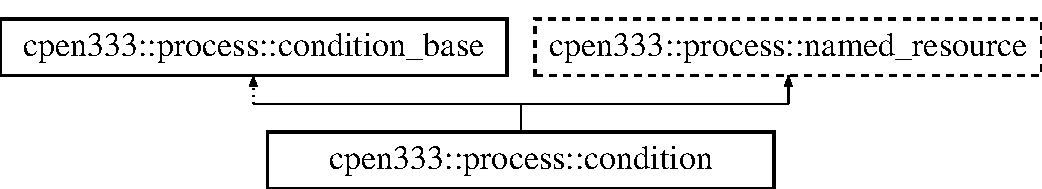
\includegraphics[height=2.000000cm]{classcpen333_1_1process_1_1condition}
\end{center}
\end{figure}
\subsection*{Public Member Functions}
\begin{DoxyCompactItemize}
\item 
\hyperlink{classcpen333_1_1process_1_1condition_a584deae08b94a2f6a49abca119183571}{condition} (const std\+::string \&name, bool value=false)
\begin{DoxyCompactList}\small\item\em Creates or connects to the named condition. \end{DoxyCompactList}\item 
void \hyperlink{classcpen333_1_1process_1_1condition_a24b3c16a8fdd333e95bf93dc07a65742}{wait} ()
\begin{DoxyCompactList}\small\item\em Waits until the condition is set. \end{DoxyCompactList}\item 
{\footnotesize template$<$class Rep , class Period $>$ }\\bool \hyperlink{classcpen333_1_1process_1_1condition_ac14bac38a3fd158af7ecf1fe5a993a40}{wait\+\_\+for} (const std\+::chrono\+::duration$<$ Rep, Period $>$ \&rel\+\_\+time)
\begin{DoxyCompactList}\small\item\em Waits for the condition to be set or for a timeout period to elapse. \end{DoxyCompactList}\item 
{\footnotesize template$<$class Clock , class Duration $>$ }\\bool \hyperlink{classcpen333_1_1process_1_1condition_a07cd864a2e089b9e1c9d468e8cd8ea62}{wait\+\_\+until} (const std\+::chrono\+::time\+\_\+point$<$ Clock, Duration $>$ \&timeout\+\_\+time)
\begin{DoxyCompactList}\small\item\em Waits for the condition to be set or for a time-\/point to be reached. \end{DoxyCompactList}\item 
void \hyperlink{classcpen333_1_1process_1_1condition_a7819f5c1e213863214a4935b0157fd8c}{notify} ()
\begin{DoxyCompactList}\small\item\em Sets the condition to {\ttfamily true} and wakes up threads. \end{DoxyCompactList}\item 
void \hyperlink{classcpen333_1_1process_1_1condition_a6b3f2a59fa85ddc3d53b60bd1a6a8556}{reset} ()
\begin{DoxyCompactList}\small\item\em Resets the condition. \end{DoxyCompactList}\item 
virtual bool \hyperlink{classcpen333_1_1process_1_1condition_a7c646204b2c4912185ba6055c9afa3f6}{unlink} ()
\begin{DoxyCompactList}\small\item\em Detaches the name from the named resource. \end{DoxyCompactList}\end{DoxyCompactItemize}
\subsection*{Static Public Member Functions}
\begin{DoxyCompactItemize}
\item 
static bool \hyperlink{classcpen333_1_1process_1_1condition_aaffc8df542fb4e2aecdc1056217a4284}{unlink} (const std\+::string \&name)
\begin{DoxyCompactList}\small\item\em Unlinks any condition with the provided name. \end{DoxyCompactList}\end{DoxyCompactItemize}


\subsection{Detailed Description}
Allows multiple processes to wait until the condition is set, acting like a gate. 

A named synchronization primitive that allows multiple threads and processes to wait until the condition is notified as being set. As long as the condition remains set, any threads that wait on the condition will immediately proceed. The condition must manually be reset in order to cause threads/processes to wait until the next time the condition is set. 

\subsection{Constructor \& Destructor Documentation}
\mbox{\Hypertarget{classcpen333_1_1process_1_1condition_a584deae08b94a2f6a49abca119183571}\label{classcpen333_1_1process_1_1condition_a584deae08b94a2f6a49abca119183571}} 
\index{cpen333\+::process\+::condition@{cpen333\+::process\+::condition}!condition@{condition}}
\index{condition@{condition}!cpen333\+::process\+::condition@{cpen333\+::process\+::condition}}
\subsubsection{\texorpdfstring{condition()}{condition()}}
{\footnotesize\ttfamily cpen333\+::process\+::condition\+::condition (\begin{DoxyParamCaption}\item[{const std\+::string \&}]{name,  }\item[{bool}]{value = {\ttfamily false} }\end{DoxyParamCaption})\hspace{0.3cm}{\ttfamily [inline]}}



Creates or connects to the named condition. 


\begin{DoxyParams}{Parameters}
{\em name} & name identifier for creating or connecting to an existing inter-\/process condition \\
\hline
{\em value} & initial state, as either set ({\ttfamily true}) or reset ({\ttfamily false}) \\
\hline
\end{DoxyParams}


\subsection{Member Function Documentation}
\mbox{\Hypertarget{classcpen333_1_1process_1_1condition_a7819f5c1e213863214a4935b0157fd8c}\label{classcpen333_1_1process_1_1condition_a7819f5c1e213863214a4935b0157fd8c}} 
\index{cpen333\+::process\+::condition@{cpen333\+::process\+::condition}!notify@{notify}}
\index{notify@{notify}!cpen333\+::process\+::condition@{cpen333\+::process\+::condition}}
\subsubsection{\texorpdfstring{notify()}{notify()}}
{\footnotesize\ttfamily void cpen333\+::process\+::condition\+::notify (\begin{DoxyParamCaption}{ }\end{DoxyParamCaption})\hspace{0.3cm}{\ttfamily [inline]}}



Sets the condition to {\ttfamily true} and wakes up threads. 

Sets the condition\textquotesingle{}s internal state to {\ttfamily true} and wakes up any threads waiting on the condition. The condition will remain in the {\ttfamily set} state until it is manually reset. \mbox{\Hypertarget{classcpen333_1_1process_1_1condition_a6b3f2a59fa85ddc3d53b60bd1a6a8556}\label{classcpen333_1_1process_1_1condition_a6b3f2a59fa85ddc3d53b60bd1a6a8556}} 
\index{cpen333\+::process\+::condition@{cpen333\+::process\+::condition}!reset@{reset}}
\index{reset@{reset}!cpen333\+::process\+::condition@{cpen333\+::process\+::condition}}
\subsubsection{\texorpdfstring{reset()}{reset()}}
{\footnotesize\ttfamily void cpen333\+::process\+::condition\+::reset (\begin{DoxyParamCaption}{ }\end{DoxyParamCaption})\hspace{0.3cm}{\ttfamily [inline]}}



Resets the condition. 

Sets the condition\textquotesingle{}s internal state to {\ttfamily false}. This will call any future {\ttfamily wait} calls to block until the condition is again notified. \mbox{\Hypertarget{classcpen333_1_1process_1_1condition_a7c646204b2c4912185ba6055c9afa3f6}\label{classcpen333_1_1process_1_1condition_a7c646204b2c4912185ba6055c9afa3f6}} 
\index{cpen333\+::process\+::condition@{cpen333\+::process\+::condition}!unlink@{unlink}}
\index{unlink@{unlink}!cpen333\+::process\+::condition@{cpen333\+::process\+::condition}}
\subsubsection{\texorpdfstring{unlink()}{unlink()}\hspace{0.1cm}{\footnotesize\ttfamily [1/2]}}
{\footnotesize\ttfamily virtual bool cpen333\+::process\+::condition\+::unlink (\begin{DoxyParamCaption}{ }\end{DoxyParamCaption})\hspace{0.3cm}{\ttfamily [inline]}, {\ttfamily [virtual]}}



Detaches the name from the named resource. 

On P\+O\+S\+IX systems, named resources will persist beyond the lifetime of any process that uses them as long as the name has not been unlinked (or until the system is rebooted). Calling {\ttfamily unlink} will detach the name, allowing the resource to be freed once all current users have exited.

\begin{DoxyReturn}{Returns}
{\ttfamily true} if unlink is successful, {\ttfamily false} if unlinking is not supported or if an error has occurred. 
\end{DoxyReturn}


Reimplemented from \hyperlink{classcpen333_1_1process_1_1condition__base_acd6d0b53a828aa161ccad06885eaa15c}{cpen333\+::process\+::condition\+\_\+base}.

\mbox{\Hypertarget{classcpen333_1_1process_1_1condition_aaffc8df542fb4e2aecdc1056217a4284}\label{classcpen333_1_1process_1_1condition_aaffc8df542fb4e2aecdc1056217a4284}} 
\index{cpen333\+::process\+::condition@{cpen333\+::process\+::condition}!unlink@{unlink}}
\index{unlink@{unlink}!cpen333\+::process\+::condition@{cpen333\+::process\+::condition}}
\subsubsection{\texorpdfstring{unlink()}{unlink()}\hspace{0.1cm}{\footnotesize\ttfamily [2/2]}}
{\footnotesize\ttfamily static bool cpen333\+::process\+::condition\+::unlink (\begin{DoxyParamCaption}\item[{const std\+::string \&}]{name }\end{DoxyParamCaption})\hspace{0.3cm}{\ttfamily [inline]}, {\ttfamily [static]}}



Unlinks any condition with the provided name. 

Allows a name to be freed without needing to create a new condition resource. This is useful for clean-\/up of previously terminated processes that failed to release the resource properly.


\begin{DoxyParams}{Parameters}
{\em name} & name of condition resource \\
\hline
\end{DoxyParams}
\begin{DoxyReturn}{Returns}
{\ttfamily true} if unlink successful, {\ttfamily false} if an error occurred or if not supported 
\end{DoxyReturn}
\mbox{\Hypertarget{classcpen333_1_1process_1_1condition_a24b3c16a8fdd333e95bf93dc07a65742}\label{classcpen333_1_1process_1_1condition_a24b3c16a8fdd333e95bf93dc07a65742}} 
\index{cpen333\+::process\+::condition@{cpen333\+::process\+::condition}!wait@{wait}}
\index{wait@{wait}!cpen333\+::process\+::condition@{cpen333\+::process\+::condition}}
\subsubsection{\texorpdfstring{wait()}{wait()}}
{\footnotesize\ttfamily void cpen333\+::process\+::condition\+::wait (\begin{DoxyParamCaption}{ }\end{DoxyParamCaption})\hspace{0.3cm}{\ttfamily [inline]}}



Waits until the condition is set. 

Causes the current thread to block until the condition is set. This condition will {\itshape not} exhibit spurious wake-\/ups. A thread will be forced to wait here indefinitely until the condition is set. \mbox{\Hypertarget{classcpen333_1_1process_1_1condition_ac14bac38a3fd158af7ecf1fe5a993a40}\label{classcpen333_1_1process_1_1condition_ac14bac38a3fd158af7ecf1fe5a993a40}} 
\index{cpen333\+::process\+::condition@{cpen333\+::process\+::condition}!wait\+\_\+for@{wait\+\_\+for}}
\index{wait\+\_\+for@{wait\+\_\+for}!cpen333\+::process\+::condition@{cpen333\+::process\+::condition}}
\subsubsection{\texorpdfstring{wait\+\_\+for()}{wait\_for()}}
{\footnotesize\ttfamily template$<$class Rep , class Period $>$ \\
bool cpen333\+::process\+::condition\+::wait\+\_\+for (\begin{DoxyParamCaption}\item[{const std\+::chrono\+::duration$<$ Rep, Period $>$ \&}]{rel\+\_\+time }\end{DoxyParamCaption})\hspace{0.3cm}{\ttfamily [inline]}}



Waits for the condition to be set or for a timeout period to elapse. 

Causes the current thread to block until the condition is set, or until the specified timeout period elapses, whichever comes first. 
\begin{DoxyTemplParams}{Template Parameters}
{\em Rep} & timeout duration representation \\
\hline
{\em Period} & timeout clock period \\
\hline
\end{DoxyTemplParams}

\begin{DoxyParams}{Parameters}
{\em rel\+\_\+time} & maximum relative time to wait for condition to be set \\
\hline
\end{DoxyParams}
\begin{DoxyReturn}{Returns}
{\ttfamily true} if condition is set, {\ttfamily false} if timeout has elapsed without condition being set 
\end{DoxyReturn}
\mbox{\Hypertarget{classcpen333_1_1process_1_1condition_a07cd864a2e089b9e1c9d468e8cd8ea62}\label{classcpen333_1_1process_1_1condition_a07cd864a2e089b9e1c9d468e8cd8ea62}} 
\index{cpen333\+::process\+::condition@{cpen333\+::process\+::condition}!wait\+\_\+until@{wait\+\_\+until}}
\index{wait\+\_\+until@{wait\+\_\+until}!cpen333\+::process\+::condition@{cpen333\+::process\+::condition}}
\subsubsection{\texorpdfstring{wait\+\_\+until()}{wait\_until()}}
{\footnotesize\ttfamily template$<$class Clock , class Duration $>$ \\
bool cpen333\+::process\+::condition\+::wait\+\_\+until (\begin{DoxyParamCaption}\item[{const std\+::chrono\+::time\+\_\+point$<$ Clock, Duration $>$ \&}]{timeout\+\_\+time }\end{DoxyParamCaption})\hspace{0.3cm}{\ttfamily [inline]}}



Waits for the condition to be set or for a time-\/point to be reached. 

Causes the current thread to block until the condition is set, or until the specified timeout time has been reached, whichever comes first.


\begin{DoxyTemplParams}{Template Parameters}
{\em Clock} & clock type \\
\hline
{\em Duration} & clock duration type \\
\hline
\end{DoxyTemplParams}

\begin{DoxyParams}{Parameters}
{\em timeout\+\_\+time} & absolute timeout time \\
\hline
\end{DoxyParams}
\begin{DoxyReturn}{Returns}
{\ttfamily true} if condition is set, {\ttfamily false} if timeout time has been reached without condition being set 
\end{DoxyReturn}


The documentation for this class was generated from the following file\+:\begin{DoxyCompactItemize}
\item 
D\+:/school/teaching/\+C\+P\+E\+N333/workspace/labs/include/cpen333/process/\hyperlink{process_2condition_8h}{condition.\+h}\end{DoxyCompactItemize}

\hypertarget{classcpen333_1_1thread_1_1condition}{}\section{cpen333\+:\+:thread\+:\+:condition Class Reference}
\label{classcpen333_1_1thread_1_1condition}\index{cpen333\+::thread\+::condition@{cpen333\+::thread\+::condition}}


Allows multiple threads to wait until the condition is set, acting like a gate.  




{\ttfamily \#include $<$condition.\+h$>$}

\subsection*{Public Member Functions}
\begin{DoxyCompactItemize}
\item 
\hyperlink{classcpen333_1_1thread_1_1condition_a3bd725835dd906ab14b7796cb425fe71}{condition} (bool value=false)
\begin{DoxyCompactList}\small\item\em Creates the condition. \end{DoxyCompactList}\item 
void \hyperlink{classcpen333_1_1thread_1_1condition_a8f04e3bd62b29535f8a98ded4efafea2}{wait} ()
\begin{DoxyCompactList}\small\item\em Waits until the condition is set. \end{DoxyCompactList}\item 
{\footnotesize template$<$class Rep , class Period $>$ }\\bool \hyperlink{classcpen333_1_1thread_1_1condition_a14464ca04c1e3e4a6ae62321bfe1ad3a}{wait\+\_\+for} (const std\+::chrono\+::duration$<$ Rep, Period $>$ \&rel\+\_\+time)
\begin{DoxyCompactList}\small\item\em Waits for the condition to be set or for a timeout period to elapse. \end{DoxyCompactList}\item 
{\footnotesize template$<$class Clock , class Duration $>$ }\\bool \hyperlink{classcpen333_1_1thread_1_1condition_ad415e3be6db8f186d2efaa1c897ffca5}{wait\+\_\+until} (const std\+::chrono\+::time\+\_\+point$<$ Clock, Duration $>$ \&timeout\+\_\+time)
\begin{DoxyCompactList}\small\item\em Waits for the condition to be set or for a time-\/point to be reached. \end{DoxyCompactList}\item 
void \hyperlink{classcpen333_1_1thread_1_1condition_a12be978f0adb0bf17080797a38b6ead4}{notify} ()
\begin{DoxyCompactList}\small\item\em Sets the condition to {\ttfamily true} and wakes up threads. \end{DoxyCompactList}\item 
void \hyperlink{classcpen333_1_1thread_1_1condition_a99e8696703e31632cccc1d17b0b18d2f}{reset} ()
\begin{DoxyCompactList}\small\item\em Resets the condition. \end{DoxyCompactList}\end{DoxyCompactItemize}


\subsection{Detailed Description}
Allows multiple threads to wait until the condition is set, acting like a gate. 

As long as the condition remains set, any threads that wait on the condition will immediately proceed. The condition must manually be reset in order to cause threads/processes to wait until the next time the condition is set. 

\subsection{Constructor \& Destructor Documentation}
\mbox{\Hypertarget{classcpen333_1_1thread_1_1condition_a3bd725835dd906ab14b7796cb425fe71}\label{classcpen333_1_1thread_1_1condition_a3bd725835dd906ab14b7796cb425fe71}} 
\index{cpen333\+::thread\+::condition@{cpen333\+::thread\+::condition}!condition@{condition}}
\index{condition@{condition}!cpen333\+::thread\+::condition@{cpen333\+::thread\+::condition}}
\subsubsection{\texorpdfstring{condition()}{condition()}}
{\footnotesize\ttfamily cpen333\+::thread\+::condition\+::condition (\begin{DoxyParamCaption}\item[{bool}]{value = {\ttfamily false} }\end{DoxyParamCaption})\hspace{0.3cm}{\ttfamily [inline]}}



Creates the condition. 


\begin{DoxyParams}{Parameters}
{\em value} & initial state, as either set ({\ttfamily true}) or reset ({\ttfamily false}) \\
\hline
\end{DoxyParams}


\subsection{Member Function Documentation}
\mbox{\Hypertarget{classcpen333_1_1thread_1_1condition_a12be978f0adb0bf17080797a38b6ead4}\label{classcpen333_1_1thread_1_1condition_a12be978f0adb0bf17080797a38b6ead4}} 
\index{cpen333\+::thread\+::condition@{cpen333\+::thread\+::condition}!notify@{notify}}
\index{notify@{notify}!cpen333\+::thread\+::condition@{cpen333\+::thread\+::condition}}
\subsubsection{\texorpdfstring{notify()}{notify()}}
{\footnotesize\ttfamily void cpen333\+::thread\+::condition\+::notify (\begin{DoxyParamCaption}{ }\end{DoxyParamCaption})\hspace{0.3cm}{\ttfamily [inline]}}



Sets the condition to {\ttfamily true} and wakes up threads. 

Sets the condition\textquotesingle{}s internal state to {\ttfamily true} and wakes up any threads waiting on the condition. The condition will remain in the {\ttfamily set} state until it is manually reset. \mbox{\Hypertarget{classcpen333_1_1thread_1_1condition_a99e8696703e31632cccc1d17b0b18d2f}\label{classcpen333_1_1thread_1_1condition_a99e8696703e31632cccc1d17b0b18d2f}} 
\index{cpen333\+::thread\+::condition@{cpen333\+::thread\+::condition}!reset@{reset}}
\index{reset@{reset}!cpen333\+::thread\+::condition@{cpen333\+::thread\+::condition}}
\subsubsection{\texorpdfstring{reset()}{reset()}}
{\footnotesize\ttfamily void cpen333\+::thread\+::condition\+::reset (\begin{DoxyParamCaption}{ }\end{DoxyParamCaption})\hspace{0.3cm}{\ttfamily [inline]}}



Resets the condition. 

Sets the condition\textquotesingle{}s internal state to {\ttfamily false}. This will call any future {\ttfamily wait} calls to block until the condition is again notified. \mbox{\Hypertarget{classcpen333_1_1thread_1_1condition_a8f04e3bd62b29535f8a98ded4efafea2}\label{classcpen333_1_1thread_1_1condition_a8f04e3bd62b29535f8a98ded4efafea2}} 
\index{cpen333\+::thread\+::condition@{cpen333\+::thread\+::condition}!wait@{wait}}
\index{wait@{wait}!cpen333\+::thread\+::condition@{cpen333\+::thread\+::condition}}
\subsubsection{\texorpdfstring{wait()}{wait()}}
{\footnotesize\ttfamily void cpen333\+::thread\+::condition\+::wait (\begin{DoxyParamCaption}{ }\end{DoxyParamCaption})\hspace{0.3cm}{\ttfamily [inline]}}



Waits until the condition is set. 

Causes the current thread to block until the condition is set. This condition will {\itshape not} exhibit spurious wake-\/ups. A thread will be forced to wait here indefinitely until the condition is set. \mbox{\Hypertarget{classcpen333_1_1thread_1_1condition_a14464ca04c1e3e4a6ae62321bfe1ad3a}\label{classcpen333_1_1thread_1_1condition_a14464ca04c1e3e4a6ae62321bfe1ad3a}} 
\index{cpen333\+::thread\+::condition@{cpen333\+::thread\+::condition}!wait\+\_\+for@{wait\+\_\+for}}
\index{wait\+\_\+for@{wait\+\_\+for}!cpen333\+::thread\+::condition@{cpen333\+::thread\+::condition}}
\subsubsection{\texorpdfstring{wait\+\_\+for()}{wait\_for()}}
{\footnotesize\ttfamily template$<$class Rep , class Period $>$ \\
bool cpen333\+::thread\+::condition\+::wait\+\_\+for (\begin{DoxyParamCaption}\item[{const std\+::chrono\+::duration$<$ Rep, Period $>$ \&}]{rel\+\_\+time }\end{DoxyParamCaption})\hspace{0.3cm}{\ttfamily [inline]}}



Waits for the condition to be set or for a timeout period to elapse. 

Causes the current thread to block until the condition is set, or until the specified timeout period elapses, whichever comes first.


\begin{DoxyTemplParams}{Template Parameters}
{\em Rep} & timeout duration representation \\
\hline
{\em Period} & timeout clock period \\
\hline
\end{DoxyTemplParams}

\begin{DoxyParams}{Parameters}
{\em rel\+\_\+time} & maximum relative time to wait for condition to be set \\
\hline
\end{DoxyParams}
\begin{DoxyReturn}{Returns}
{\ttfamily true} if condition is set, {\ttfamily false} if timeout has elapsed without condition being set 
\end{DoxyReturn}
\mbox{\Hypertarget{classcpen333_1_1thread_1_1condition_ad415e3be6db8f186d2efaa1c897ffca5}\label{classcpen333_1_1thread_1_1condition_ad415e3be6db8f186d2efaa1c897ffca5}} 
\index{cpen333\+::thread\+::condition@{cpen333\+::thread\+::condition}!wait\+\_\+until@{wait\+\_\+until}}
\index{wait\+\_\+until@{wait\+\_\+until}!cpen333\+::thread\+::condition@{cpen333\+::thread\+::condition}}
\subsubsection{\texorpdfstring{wait\+\_\+until()}{wait\_until()}}
{\footnotesize\ttfamily template$<$class Clock , class Duration $>$ \\
bool cpen333\+::thread\+::condition\+::wait\+\_\+until (\begin{DoxyParamCaption}\item[{const std\+::chrono\+::time\+\_\+point$<$ Clock, Duration $>$ \&}]{timeout\+\_\+time }\end{DoxyParamCaption})\hspace{0.3cm}{\ttfamily [inline]}}



Waits for the condition to be set or for a time-\/point to be reached. 

Causes the current thread to block until the condition is set, or until the specified timeout time has been reached, whichever comes first.


\begin{DoxyTemplParams}{Template Parameters}
{\em Clock} & clock type \\
\hline
{\em Duration} & clock duration type \\
\hline
\end{DoxyTemplParams}

\begin{DoxyParams}{Parameters}
{\em timeout\+\_\+time} & absolute timeout time \\
\hline
\end{DoxyParams}
\begin{DoxyReturn}{Returns}
{\ttfamily true} if condition is set, {\ttfamily false} if timeout time has been reached without condition being set 
\end{DoxyReturn}


The documentation for this class was generated from the following file\+:\begin{DoxyCompactItemize}
\item 
D\+:/school/teaching/\+C\+P\+E\+N333/workspace/labs/include/cpen333/thread/\hyperlink{thread_2condition_8h}{condition.\+h}\end{DoxyCompactItemize}

\hypertarget{classcpen333_1_1process_1_1condition__base}{}\section{cpen333\+:\+:process\+:\+:condition\+\_\+base Class Reference}
\label{classcpen333_1_1process_1_1condition__base}\index{cpen333\+::process\+::condition\+\_\+base@{cpen333\+::process\+::condition\+\_\+base}}


Base-\/class for conditions, condition variables, and events.  




{\ttfamily \#include $<$condition\+\_\+base.\+h$>$}

Inheritance diagram for cpen333\+:\+:process\+:\+:condition\+\_\+base\+:\begin{figure}[H]
\begin{center}
\leavevmode
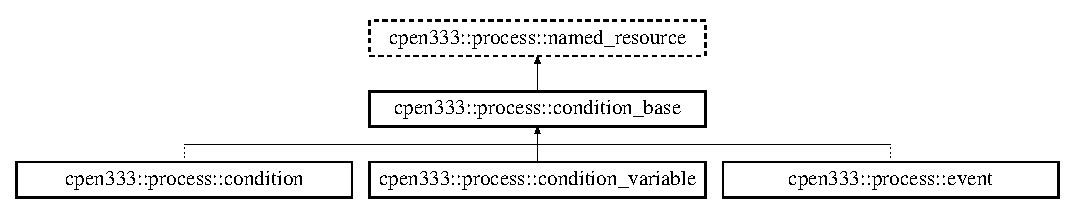
\includegraphics[height=2.434783cm]{classcpen333_1_1process_1_1condition__base}
\end{center}
\end{figure}
\subsection*{Public Member Functions}
\begin{DoxyCompactItemize}
\item 
\hyperlink{classcpen333_1_1process_1_1condition__base_a23384ba303cc2111cc4272830ae9f72b}{condition\+\_\+base} (const std\+::string \&name)
\begin{DoxyCompactList}\small\item\em Constructor. \end{DoxyCompactList}\item 
void \hyperlink{classcpen333_1_1process_1_1condition__base_a29b67e4579cef831f709ea4c3a32ffe5}{wait} (std\+::unique\+\_\+lock$<$ \hyperlink{classcpen333_1_1process_1_1mutex}{cpen333\+::process\+::mutex} $>$ \&lock)
\begin{DoxyCompactList}\small\item\em Wait until the thread is notified. \end{DoxyCompactList}\item 
{\footnotesize template$<$class Rep , class Period $>$ }\\bool \hyperlink{classcpen333_1_1process_1_1condition__base_ab19d033fcec20cd7f2a3f0b38e67a19d}{wait\+\_\+for} (std\+::unique\+\_\+lock$<$ \hyperlink{classcpen333_1_1process_1_1mutex}{cpen333\+::process\+::mutex} $>$ \&lock, const std\+::chrono\+::duration$<$ Rep, Period $>$ \&rel\+\_\+time)
\begin{DoxyCompactList}\small\item\em Wait until the thread is notified, or until a timeout period has elapsed. \end{DoxyCompactList}\item 
{\footnotesize template$<$class Clock , class Duration $>$ }\\bool \hyperlink{classcpen333_1_1process_1_1condition__base_a6af33a75565bf4177cb6616a08acaac0}{wait\+\_\+until} (std\+::unique\+\_\+lock$<$ \hyperlink{classcpen333_1_1process_1_1mutex}{cpen333\+::process\+::mutex} $>$ \&lock, const std\+::chrono\+::time\+\_\+point$<$ Clock, Duration $>$ \&timeout\+\_\+time)
\begin{DoxyCompactList}\small\item\em Wait until the thread is notified, or until a timeout time has been reached. \end{DoxyCompactList}\item 
void \hyperlink{classcpen333_1_1process_1_1condition__base_a990220c8ee064b3d494cdbf238ceb73e}{notify\+\_\+one} ()
\begin{DoxyCompactList}\small\item\em Notify one waiting thread. \end{DoxyCompactList}\item 
void \hyperlink{classcpen333_1_1process_1_1condition__base_a37b38d480898c0cc13b0ea1eb2b24127}{notify\+\_\+all} ()
\begin{DoxyCompactList}\small\item\em Notify all waiting threads. \end{DoxyCompactList}\item 
virtual bool \hyperlink{classcpen333_1_1process_1_1condition__base_acd6d0b53a828aa161ccad06885eaa15c}{unlink} ()
\begin{DoxyCompactList}\small\item\em Detaches the name from the named resource. \end{DoxyCompactList}\end{DoxyCompactItemize}
\subsection*{Static Public Member Functions}
\begin{DoxyCompactItemize}
\item 
static bool \hyperlink{classcpen333_1_1process_1_1condition__base_a01ed2d247732584166613527ea8e1aff}{unlink} (const std\+::string \&name)
\begin{DoxyCompactList}\small\item\em Unlinks the name without needing to create a resource. \end{DoxyCompactList}\end{DoxyCompactItemize}
\subsection*{Protected Member Functions}
\begin{DoxyCompactItemize}
\item 
void \hyperlink{classcpen333_1_1process_1_1condition__base_af6f7110f5be9935ac2fbea2b303a2903}{notify} (bool broadcast)
\begin{DoxyCompactList}\small\item\em Notify (wake-\/up) waiting threads. \end{DoxyCompactList}\item 
{\footnotesize template$<$class Clock , class Duration $>$ }\\bool \hyperlink{classcpen333_1_1process_1_1condition__base_a3132db3bcedcddf3a8e5ac24df8d9efa}{wait} (std\+::unique\+\_\+lock$<$ \hyperlink{classcpen333_1_1process_1_1mutex}{cpen333\+::process\+::mutex} $>$ \&lock, bool timeout, const std\+::chrono\+::time\+\_\+point$<$ Clock, Duration $>$ \&abs\+\_\+time)
\begin{DoxyCompactList}\small\item\em Waits for condition to be notified. \end{DoxyCompactList}\end{DoxyCompactItemize}


\subsection{Detailed Description}
Base-\/class for conditions, condition variables, and events. 

Like an event, has the ability to wait for ownership of a lock, and for notifying waiting threads. This condition base D\+O\+ES N\+OT suffer from spurious wake-\/ups. 

\subsection{Constructor \& Destructor Documentation}
\mbox{\Hypertarget{classcpen333_1_1process_1_1condition__base_a23384ba303cc2111cc4272830ae9f72b}\label{classcpen333_1_1process_1_1condition__base_a23384ba303cc2111cc4272830ae9f72b}} 
\index{cpen333\+::process\+::condition\+\_\+base@{cpen333\+::process\+::condition\+\_\+base}!condition\+\_\+base@{condition\+\_\+base}}
\index{condition\+\_\+base@{condition\+\_\+base}!cpen333\+::process\+::condition\+\_\+base@{cpen333\+::process\+::condition\+\_\+base}}
\subsubsection{\texorpdfstring{condition\+\_\+base()}{condition\_base()}}
{\footnotesize\ttfamily cpen333\+::process\+::condition\+\_\+base\+::condition\+\_\+base (\begin{DoxyParamCaption}\item[{const std\+::string \&}]{name }\end{DoxyParamCaption})\hspace{0.3cm}{\ttfamily [inline]}}



Constructor. 


\begin{DoxyParams}{Parameters}
{\em name} & unique identifier \\
\hline
\end{DoxyParams}


\subsection{Member Function Documentation}
\mbox{\Hypertarget{classcpen333_1_1process_1_1condition__base_af6f7110f5be9935ac2fbea2b303a2903}\label{classcpen333_1_1process_1_1condition__base_af6f7110f5be9935ac2fbea2b303a2903}} 
\index{cpen333\+::process\+::condition\+\_\+base@{cpen333\+::process\+::condition\+\_\+base}!notify@{notify}}
\index{notify@{notify}!cpen333\+::process\+::condition\+\_\+base@{cpen333\+::process\+::condition\+\_\+base}}
\subsubsection{\texorpdfstring{notify()}{notify()}}
{\footnotesize\ttfamily void cpen333\+::process\+::condition\+\_\+base\+::notify (\begin{DoxyParamCaption}\item[{bool}]{broadcast }\end{DoxyParamCaption})\hspace{0.3cm}{\ttfamily [inline]}, {\ttfamily [protected]}}



Notify (wake-\/up) waiting threads. 


\begin{DoxyParams}{Parameters}
{\em broadcast} & if true, wakes up all threads \\
\hline
\end{DoxyParams}
\mbox{\Hypertarget{classcpen333_1_1process_1_1condition__base_a37b38d480898c0cc13b0ea1eb2b24127}\label{classcpen333_1_1process_1_1condition__base_a37b38d480898c0cc13b0ea1eb2b24127}} 
\index{cpen333\+::process\+::condition\+\_\+base@{cpen333\+::process\+::condition\+\_\+base}!notify\+\_\+all@{notify\+\_\+all}}
\index{notify\+\_\+all@{notify\+\_\+all}!cpen333\+::process\+::condition\+\_\+base@{cpen333\+::process\+::condition\+\_\+base}}
\subsubsection{\texorpdfstring{notify\+\_\+all()}{notify\_all()}}
{\footnotesize\ttfamily void cpen333\+::process\+::condition\+\_\+base\+::notify\+\_\+all (\begin{DoxyParamCaption}{ }\end{DoxyParamCaption})\hspace{0.3cm}{\ttfamily [inline]}}



Notify all waiting threads. 

Wake up all waiting threads and notify them of a potential change \mbox{\Hypertarget{classcpen333_1_1process_1_1condition__base_a990220c8ee064b3d494cdbf238ceb73e}\label{classcpen333_1_1process_1_1condition__base_a990220c8ee064b3d494cdbf238ceb73e}} 
\index{cpen333\+::process\+::condition\+\_\+base@{cpen333\+::process\+::condition\+\_\+base}!notify\+\_\+one@{notify\+\_\+one}}
\index{notify\+\_\+one@{notify\+\_\+one}!cpen333\+::process\+::condition\+\_\+base@{cpen333\+::process\+::condition\+\_\+base}}
\subsubsection{\texorpdfstring{notify\+\_\+one()}{notify\_one()}}
{\footnotesize\ttfamily void cpen333\+::process\+::condition\+\_\+base\+::notify\+\_\+one (\begin{DoxyParamCaption}{ }\end{DoxyParamCaption})\hspace{0.3cm}{\ttfamily [inline]}}



Notify one waiting thread. 

Wake up a single waiting thread and notify them of a potential change \mbox{\Hypertarget{classcpen333_1_1process_1_1condition__base_acd6d0b53a828aa161ccad06885eaa15c}\label{classcpen333_1_1process_1_1condition__base_acd6d0b53a828aa161ccad06885eaa15c}} 
\index{cpen333\+::process\+::condition\+\_\+base@{cpen333\+::process\+::condition\+\_\+base}!unlink@{unlink}}
\index{unlink@{unlink}!cpen333\+::process\+::condition\+\_\+base@{cpen333\+::process\+::condition\+\_\+base}}
\subsubsection{\texorpdfstring{unlink()}{unlink()}\hspace{0.1cm}{\footnotesize\ttfamily [1/2]}}
{\footnotesize\ttfamily virtual bool cpen333\+::process\+::condition\+\_\+base\+::unlink (\begin{DoxyParamCaption}{ }\end{DoxyParamCaption})\hspace{0.3cm}{\ttfamily [inline]}, {\ttfamily [virtual]}}



Detaches the name from the named resource. 

On P\+O\+S\+IX systems, named resources will persist beyond the lifetime of any process that uses them as long as the name has not been unlinked (or until the system is rebooted). Calling {\ttfamily unlink} will detach the name, allowing the resource to be freed once all current users have exited.

\begin{DoxyReturn}{Returns}
{\ttfamily true} if unlink is successful, {\ttfamily false} if unlinking is not supported or if an error has occurred. 
\end{DoxyReturn}


Implements \hyperlink{classcpen333_1_1process_1_1named__resource_a5d33168fee48c9b0c58ab8fd96e230ce}{cpen333\+::process\+::named\+\_\+resource}.



Reimplemented in \hyperlink{classcpen333_1_1process_1_1condition__variable_a2861ec071acc52be7ca5790edd062ee8}{cpen333\+::process\+::condition\+\_\+variable}, \hyperlink{classcpen333_1_1process_1_1condition_a7c646204b2c4912185ba6055c9afa3f6}{cpen333\+::process\+::condition}, and \hyperlink{classcpen333_1_1process_1_1event_a37a2d53cbf4a90da6b4dbd5853f23b32}{cpen333\+::process\+::event}.

\mbox{\Hypertarget{classcpen333_1_1process_1_1condition__base_a01ed2d247732584166613527ea8e1aff}\label{classcpen333_1_1process_1_1condition__base_a01ed2d247732584166613527ea8e1aff}} 
\index{cpen333\+::process\+::condition\+\_\+base@{cpen333\+::process\+::condition\+\_\+base}!unlink@{unlink}}
\index{unlink@{unlink}!cpen333\+::process\+::condition\+\_\+base@{cpen333\+::process\+::condition\+\_\+base}}
\subsubsection{\texorpdfstring{unlink()}{unlink()}\hspace{0.1cm}{\footnotesize\ttfamily [2/2]}}
{\footnotesize\ttfamily static bool cpen333\+::process\+::condition\+\_\+base\+::unlink (\begin{DoxyParamCaption}\item[{const std\+::string \&}]{name }\end{DoxyParamCaption})\hspace{0.3cm}{\ttfamily [inline]}, {\ttfamily [static]}}



Unlinks the name without needing to create a resource. 

Implementers should also provide a static method for unlinking. The purpose is mainly for clean-\/up of existing resources.


\begin{DoxyParams}{Parameters}
{\em name} & desired resource name \\
\hline
\end{DoxyParams}
\begin{DoxyReturn}{Returns}
{\ttfamily true} if unlink successful, {\ttfamily false} if not successful or not supported 
\end{DoxyReturn}
\mbox{\Hypertarget{classcpen333_1_1process_1_1condition__base_a29b67e4579cef831f709ea4c3a32ffe5}\label{classcpen333_1_1process_1_1condition__base_a29b67e4579cef831f709ea4c3a32ffe5}} 
\index{cpen333\+::process\+::condition\+\_\+base@{cpen333\+::process\+::condition\+\_\+base}!wait@{wait}}
\index{wait@{wait}!cpen333\+::process\+::condition\+\_\+base@{cpen333\+::process\+::condition\+\_\+base}}
\subsubsection{\texorpdfstring{wait()}{wait()}\hspace{0.1cm}{\footnotesize\ttfamily [1/2]}}
{\footnotesize\ttfamily void cpen333\+::process\+::condition\+\_\+base\+::wait (\begin{DoxyParamCaption}\item[{std\+::unique\+\_\+lock$<$ \hyperlink{classcpen333_1_1process_1_1mutex}{cpen333\+::process\+::mutex} $>$ \&}]{lock }\end{DoxyParamCaption})\hspace{0.3cm}{\ttfamily [inline]}}



Wait until the thread is notified. 


\begin{DoxyParams}{Parameters}
{\em lock} & external lock \\
\hline
\end{DoxyParams}
\mbox{\Hypertarget{classcpen333_1_1process_1_1condition__base_a3132db3bcedcddf3a8e5ac24df8d9efa}\label{classcpen333_1_1process_1_1condition__base_a3132db3bcedcddf3a8e5ac24df8d9efa}} 
\index{cpen333\+::process\+::condition\+\_\+base@{cpen333\+::process\+::condition\+\_\+base}!wait@{wait}}
\index{wait@{wait}!cpen333\+::process\+::condition\+\_\+base@{cpen333\+::process\+::condition\+\_\+base}}
\subsubsection{\texorpdfstring{wait()}{wait()}\hspace{0.1cm}{\footnotesize\ttfamily [2/2]}}
{\footnotesize\ttfamily template$<$class Clock , class Duration $>$ \\
bool cpen333\+::process\+::condition\+\_\+base\+::wait (\begin{DoxyParamCaption}\item[{std\+::unique\+\_\+lock$<$ \hyperlink{classcpen333_1_1process_1_1mutex}{cpen333\+::process\+::mutex} $>$ \&}]{lock,  }\item[{bool}]{timeout,  }\item[{const std\+::chrono\+::time\+\_\+point$<$ Clock, Duration $>$ \&}]{abs\+\_\+time }\end{DoxyParamCaption})\hspace{0.3cm}{\ttfamily [inline]}, {\ttfamily [protected]}}



Waits for condition to be notified. 


\begin{DoxyTemplParams}{Template Parameters}
{\em Clock} & clock type \\
\hline
{\em Duration} & duration type \\
\hline
\end{DoxyTemplParams}

\begin{DoxyParams}{Parameters}
{\em lock} & external lock to ensure no simultaneous waits/notifies \\
\hline
{\em timeout} & whether or not to wait with a timeout \\
\hline
{\em abs\+\_\+time} & absolute timeout time \\
\hline
\end{DoxyParams}
\begin{DoxyReturn}{Returns}
true if wait was successful, false if timeout occurred 
\end{DoxyReturn}
\mbox{\Hypertarget{classcpen333_1_1process_1_1condition__base_ab19d033fcec20cd7f2a3f0b38e67a19d}\label{classcpen333_1_1process_1_1condition__base_ab19d033fcec20cd7f2a3f0b38e67a19d}} 
\index{cpen333\+::process\+::condition\+\_\+base@{cpen333\+::process\+::condition\+\_\+base}!wait\+\_\+for@{wait\+\_\+for}}
\index{wait\+\_\+for@{wait\+\_\+for}!cpen333\+::process\+::condition\+\_\+base@{cpen333\+::process\+::condition\+\_\+base}}
\subsubsection{\texorpdfstring{wait\+\_\+for()}{wait\_for()}}
{\footnotesize\ttfamily template$<$class Rep , class Period $>$ \\
bool cpen333\+::process\+::condition\+\_\+base\+::wait\+\_\+for (\begin{DoxyParamCaption}\item[{std\+::unique\+\_\+lock$<$ \hyperlink{classcpen333_1_1process_1_1mutex}{cpen333\+::process\+::mutex} $>$ \&}]{lock,  }\item[{const std\+::chrono\+::duration$<$ Rep, Period $>$ \&}]{rel\+\_\+time }\end{DoxyParamCaption})\hspace{0.3cm}{\ttfamily [inline]}}



Wait until the thread is notified, or until a timeout period has elapsed. 


\begin{DoxyTemplParams}{Template Parameters}
{\em Rep} & duration clock representation \\
\hline
{\em Period} & duration clock period \\
\hline
\end{DoxyTemplParams}

\begin{DoxyParams}{Parameters}
{\em lock} & external lock \\
\hline
{\em rel\+\_\+time} & relative time to wait \\
\hline
\end{DoxyParams}
\begin{DoxyReturn}{Returns}
true if successful, false iftimeout has occured 
\end{DoxyReturn}
\mbox{\Hypertarget{classcpen333_1_1process_1_1condition__base_a6af33a75565bf4177cb6616a08acaac0}\label{classcpen333_1_1process_1_1condition__base_a6af33a75565bf4177cb6616a08acaac0}} 
\index{cpen333\+::process\+::condition\+\_\+base@{cpen333\+::process\+::condition\+\_\+base}!wait\+\_\+until@{wait\+\_\+until}}
\index{wait\+\_\+until@{wait\+\_\+until}!cpen333\+::process\+::condition\+\_\+base@{cpen333\+::process\+::condition\+\_\+base}}
\subsubsection{\texorpdfstring{wait\+\_\+until()}{wait\_until()}}
{\footnotesize\ttfamily template$<$class Clock , class Duration $>$ \\
bool cpen333\+::process\+::condition\+\_\+base\+::wait\+\_\+until (\begin{DoxyParamCaption}\item[{std\+::unique\+\_\+lock$<$ \hyperlink{classcpen333_1_1process_1_1mutex}{cpen333\+::process\+::mutex} $>$ \&}]{lock,  }\item[{const std\+::chrono\+::time\+\_\+point$<$ Clock, Duration $>$ \&}]{timeout\+\_\+time }\end{DoxyParamCaption})\hspace{0.3cm}{\ttfamily [inline]}}



Wait until the thread is notified, or until a timeout time has been reached. 


\begin{DoxyTemplParams}{Template Parameters}
{\em Clock} & timeout clock representation \\
\hline
{\em Duration} & timeout duration \\
\hline
\end{DoxyTemplParams}

\begin{DoxyParams}{Parameters}
{\em lock} & external lock \\
\hline
{\em timeout\+\_\+time} & absolute timeout time \\
\hline
\end{DoxyParams}
\begin{DoxyReturn}{Returns}
true if wait is successful, false if timeout has been reached 
\end{DoxyReturn}


The documentation for this class was generated from the following file\+:\begin{DoxyCompactItemize}
\item 
D\+:/school/teaching/\+C\+P\+E\+N333/workspace/library/include/cpen333/process/impl/\hyperlink{condition__base_8h}{condition\+\_\+base.\+h}\end{DoxyCompactItemize}

\hypertarget{classcpen333_1_1process_1_1condition__variable}{}\section{cpen333\+:\+:process\+:\+:condition\+\_\+variable Class Reference}
\label{classcpen333_1_1process_1_1condition__variable}\index{cpen333\+::process\+::condition\+\_\+variable@{cpen333\+::process\+::condition\+\_\+variable}}


Allows multiple process to wait for a condition to become {\ttfamily true} depending on a shared variable.  




{\ttfamily \#include $<$condition\+\_\+variable.\+h$>$}

Inheritance diagram for cpen333\+:\+:process\+:\+:condition\+\_\+variable\+:\begin{figure}[H]
\begin{center}
\leavevmode
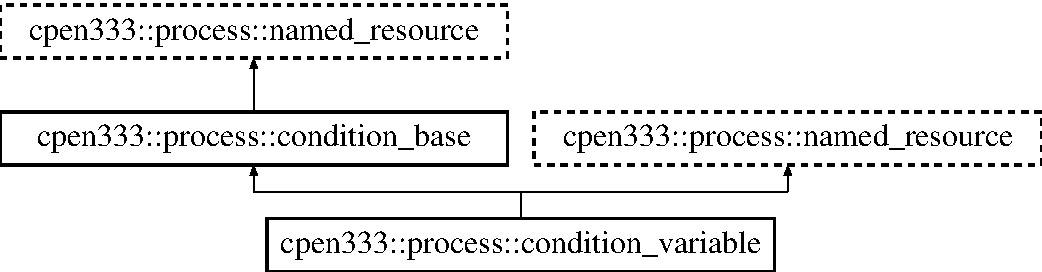
\includegraphics[height=3.000000cm]{classcpen333_1_1process_1_1condition__variable}
\end{center}
\end{figure}
\subsection*{Public Member Functions}
\begin{DoxyCompactItemize}
\item 
\hyperlink{classcpen333_1_1process_1_1condition__variable_a7f43a5fdf856a56f1e992117fc4e45c3}{condition\+\_\+variable} (const std\+::string \&name)
\begin{DoxyCompactList}\small\item\em Creates or connects to a named condition variable. \end{DoxyCompactList}\item 
void \hyperlink{classcpen333_1_1process_1_1condition__variable_ae5b7ef264d9618986be69d5c0c488925}{wait} (std\+::unique\+\_\+lock$<$ \hyperlink{classcpen333_1_1process_1_1mutex}{cpen333\+::process\+::mutex} $>$ \&lock)
\begin{DoxyCompactList}\small\item\em Waits until the \hyperlink{classcpen333_1_1process_1_1condition__variable}{condition\+\_\+variable} is notified. \end{DoxyCompactList}\item 
{\footnotesize template$<$class Rep , class Period $>$ }\\std\+::cv\+\_\+status \hyperlink{classcpen333_1_1process_1_1condition__variable_a6c6f153853d2c8d455781f0c35fdcb3b}{wait\+\_\+for} (std\+::unique\+\_\+lock$<$ \hyperlink{classcpen333_1_1process_1_1mutex}{cpen333\+::process\+::mutex} $>$ \&lock, const std\+::chrono\+::duration$<$ Rep, Period $>$ \&rel\+\_\+time)
\begin{DoxyCompactList}\small\item\em Waits for the \hyperlink{classcpen333_1_1process_1_1condition__variable}{condition\+\_\+variable} to be notified or for a timeout period to elapse. \end{DoxyCompactList}\item 
{\footnotesize template$<$class Clock , class Duration $>$ }\\bool \hyperlink{classcpen333_1_1process_1_1condition__variable_a20affb59c611bd2577e940ba5193d801}{wait\+\_\+until} (std\+::unique\+\_\+lock$<$ \hyperlink{classcpen333_1_1process_1_1mutex}{cpen333\+::process\+::mutex} $>$ \&lock, const std\+::chrono\+::time\+\_\+point$<$ Clock, Duration $>$ \&timeout\+\_\+time)
\begin{DoxyCompactList}\small\item\em Waits for the \hyperlink{classcpen333_1_1process_1_1condition__variable}{condition\+\_\+variable} to be notified or for a time-\/point to be reached. \end{DoxyCompactList}\item 
{\footnotesize template$<$typename Predicate $>$ }\\void \hyperlink{classcpen333_1_1process_1_1condition__variable_a17c52558451f262f411da1944319eb46}{wait} (std\+::unique\+\_\+lock$<$ \hyperlink{classcpen333_1_1process_1_1mutex}{cpen333\+::process\+::mutex} $>$ \&lock, Predicate pred)
\begin{DoxyCompactList}\small\item\em Waits for the \hyperlink{classcpen333_1_1process_1_1condition__variable}{condition\+\_\+variable} to be notified and the predicate {\ttfamily pred()} to evaluate to {\ttfamily true}. \end{DoxyCompactList}\item 
{\footnotesize template$<$class Rep , class Period , class Predicate $>$ }\\bool \hyperlink{classcpen333_1_1process_1_1condition__variable_af610e3f28f9c5ea4c24b35cca125ff45}{wait\+\_\+for} (std\+::unique\+\_\+lock$<$ \hyperlink{classcpen333_1_1process_1_1mutex}{cpen333\+::process\+::mutex} $>$ \&lock, const std\+::chrono\+::duration$<$ Rep, Period $>$ \&rel\+\_\+time, Predicate pred)
\begin{DoxyCompactList}\small\item\em Waits for the \hyperlink{classcpen333_1_1process_1_1condition__variable}{condition\+\_\+variable} to be notified and the predicate {\ttfamily pred()} to evaluate to {\ttfamily true}, or for a timeout to elapse. \end{DoxyCompactList}\item 
{\footnotesize template$<$class Clock , class Duration , class Predicate $>$ }\\bool \hyperlink{classcpen333_1_1process_1_1condition__variable_adc559f5d5dd4af9505975c7e64d62d6e}{wait\+\_\+until} (std\+::unique\+\_\+lock$<$ \hyperlink{classcpen333_1_1process_1_1mutex}{cpen333\+::process\+::mutex} $>$ \&lock, const std\+::chrono\+::time\+\_\+point$<$ Clock, Duration $>$ \&timeout\+\_\+time, Predicate pred)
\begin{DoxyCompactList}\small\item\em Waits for the \hyperlink{classcpen333_1_1process_1_1condition__variable}{condition\+\_\+variable} to be notified and the predicate {\ttfamily pred()} to evaluate to {\ttfamily true}, or for a timeout time to be reached. \end{DoxyCompactList}\item 
bool \hyperlink{classcpen333_1_1process_1_1condition__variable_a2861ec071acc52be7ca5790edd062ee8}{unlink} ()
\begin{DoxyCompactList}\small\item\em Detaches the name from the named resource. \end{DoxyCompactList}\end{DoxyCompactItemize}
\subsection*{Static Public Member Functions}
\begin{DoxyCompactItemize}
\item 
static bool \hyperlink{classcpen333_1_1process_1_1condition__variable_aa9c5da7417ff6c6f79d8b58333e309f8}{unlink} (const std\+::string \&name)
\begin{DoxyCompactList}\small\item\em Unlinks any condition variable with the provided name. \end{DoxyCompactList}\end{DoxyCompactItemize}
\subsection*{Additional Inherited Members}


\subsection{Detailed Description}
Allows multiple process to wait for a condition to become {\ttfamily true} depending on a shared variable. 

The \hyperlink{classcpen333_1_1process_1_1condition__variable}{condition\+\_\+variable} is a named synchronization primitive that can be used to block a thread, or multiple threads, until some thread or process both modifies a shared variable (the condition), and notifies the \hyperlink{classcpen333_1_1process_1_1condition__variable}{condition\+\_\+variable}.

The thread that modifies the variable needs to 
\begin{DoxyItemize}
\item acquire a \hyperlink{classcpen333_1_1process_1_1mutex}{cpen333\+::process\+::mutex} (typically via std\+::lock\+\_\+guard) 
\item perform the modification while the lock is held 
\item execute notify\+\_\+one or notify\+\_\+all on the \hyperlink{classcpen333_1_1process_1_1condition__variable}{condition\+\_\+variable} (does not need to be under lock) 
\end{DoxyItemize}Any thread waiting under the variable needs to 
\begin{DoxyItemize}
\item acquire a std\+::unique\+\_\+lock$<$cpen333\+::process\+::mutex$>$ on the same mutex that protects the shared variable 
\item execute wait, wait\+\_\+for, or wait\+\_\+until 
\end{DoxyItemize}The wait operations atomically release the mutex and suspend the execution of the thread. When the condition variable is notified, or a timeout expires, the thread is awakened and the mutex is atomically reacquired. Unlike std\+::condition\+\_\+variable, this implementation is not prone to spurious wake-\/ups. 

\subsection{Constructor \& Destructor Documentation}
\mbox{\Hypertarget{classcpen333_1_1process_1_1condition__variable_a7f43a5fdf856a56f1e992117fc4e45c3}\label{classcpen333_1_1process_1_1condition__variable_a7f43a5fdf856a56f1e992117fc4e45c3}} 
\index{cpen333\+::process\+::condition\+\_\+variable@{cpen333\+::process\+::condition\+\_\+variable}!condition\+\_\+variable@{condition\+\_\+variable}}
\index{condition\+\_\+variable@{condition\+\_\+variable}!cpen333\+::process\+::condition\+\_\+variable@{cpen333\+::process\+::condition\+\_\+variable}}
\subsubsection{\texorpdfstring{condition\+\_\+variable()}{condition\_variable()}}
{\footnotesize\ttfamily cpen333\+::process\+::condition\+\_\+variable\+::condition\+\_\+variable (\begin{DoxyParamCaption}\item[{const std\+::string \&}]{name }\end{DoxyParamCaption})\hspace{0.3cm}{\ttfamily [inline]}}



Creates or connects to a named condition variable. 


\begin{DoxyParams}{Parameters}
{\em name} & name identifier for creating or connecting to an existing inter-\/process \hyperlink{classcpen333_1_1process_1_1condition__variable}{condition\+\_\+variable} \\
\hline
\end{DoxyParams}


\subsection{Member Function Documentation}
\mbox{\Hypertarget{classcpen333_1_1process_1_1condition__variable_a2861ec071acc52be7ca5790edd062ee8}\label{classcpen333_1_1process_1_1condition__variable_a2861ec071acc52be7ca5790edd062ee8}} 
\index{cpen333\+::process\+::condition\+\_\+variable@{cpen333\+::process\+::condition\+\_\+variable}!unlink@{unlink}}
\index{unlink@{unlink}!cpen333\+::process\+::condition\+\_\+variable@{cpen333\+::process\+::condition\+\_\+variable}}
\subsubsection{\texorpdfstring{unlink()}{unlink()}\hspace{0.1cm}{\footnotesize\ttfamily [1/2]}}
{\footnotesize\ttfamily bool cpen333\+::process\+::condition\+\_\+variable\+::unlink (\begin{DoxyParamCaption}{ }\end{DoxyParamCaption})\hspace{0.3cm}{\ttfamily [inline]}, {\ttfamily [virtual]}}



Detaches the name from the named resource. 

On P\+O\+S\+IX systems, named resources will persist beyond the lifetime of any process that uses them as long as the name has not been unlinked (or until the system is rebooted). Calling {\ttfamily unlink} will detach the name, allowing the resource to be freed once all current users have exited.

\begin{DoxyReturn}{Returns}
{\ttfamily true} if unlink is successful, {\ttfamily false} if unlinking is not supported or if an error has occurred. 
\end{DoxyReturn}


Reimplemented from \hyperlink{classcpen333_1_1process_1_1condition__base_acd6d0b53a828aa161ccad06885eaa15c}{cpen333\+::process\+::condition\+\_\+base}.

\mbox{\Hypertarget{classcpen333_1_1process_1_1condition__variable_aa9c5da7417ff6c6f79d8b58333e309f8}\label{classcpen333_1_1process_1_1condition__variable_aa9c5da7417ff6c6f79d8b58333e309f8}} 
\index{cpen333\+::process\+::condition\+\_\+variable@{cpen333\+::process\+::condition\+\_\+variable}!unlink@{unlink}}
\index{unlink@{unlink}!cpen333\+::process\+::condition\+\_\+variable@{cpen333\+::process\+::condition\+\_\+variable}}
\subsubsection{\texorpdfstring{unlink()}{unlink()}\hspace{0.1cm}{\footnotesize\ttfamily [2/2]}}
{\footnotesize\ttfamily static bool cpen333\+::process\+::condition\+\_\+variable\+::unlink (\begin{DoxyParamCaption}\item[{const std\+::string \&}]{name }\end{DoxyParamCaption})\hspace{0.3cm}{\ttfamily [inline]}, {\ttfamily [static]}}



Unlinks any condition variable with the provided name. 

Allows a name to be freed without needing to create a new \hyperlink{classcpen333_1_1process_1_1condition__variable}{condition\+\_\+variable} resource. This is useful for clean-\/up of previously terminated processes that failed to release the resource properly.


\begin{DoxyParams}{Parameters}
{\em name} & name of \hyperlink{classcpen333_1_1process_1_1condition__variable}{condition\+\_\+variable} resource \\
\hline
\end{DoxyParams}
\begin{DoxyReturn}{Returns}
{\ttfamily true} if unlink successful, {\ttfamily false} if an error occurred or if not supported 
\end{DoxyReturn}
\mbox{\Hypertarget{classcpen333_1_1process_1_1condition__variable_ae5b7ef264d9618986be69d5c0c488925}\label{classcpen333_1_1process_1_1condition__variable_ae5b7ef264d9618986be69d5c0c488925}} 
\index{cpen333\+::process\+::condition\+\_\+variable@{cpen333\+::process\+::condition\+\_\+variable}!wait@{wait}}
\index{wait@{wait}!cpen333\+::process\+::condition\+\_\+variable@{cpen333\+::process\+::condition\+\_\+variable}}
\subsubsection{\texorpdfstring{wait()}{wait()}\hspace{0.1cm}{\footnotesize\ttfamily [1/2]}}
{\footnotesize\ttfamily void cpen333\+::process\+::condition\+\_\+variable\+::wait (\begin{DoxyParamCaption}\item[{std\+::unique\+\_\+lock$<$ \hyperlink{classcpen333_1_1process_1_1mutex}{cpen333\+::process\+::mutex} $>$ \&}]{lock }\end{DoxyParamCaption})\hspace{0.3cm}{\ttfamily [inline]}}



Waits until the \hyperlink{classcpen333_1_1process_1_1condition__variable}{condition\+\_\+variable} is notified. 

The current thread will block until the shared \hyperlink{classcpen333_1_1process_1_1condition__variable}{condition\+\_\+variable} is explicitly notified. The lock must be acquired before the wait command. As the thread is suspended, it will atomically release the lock. When it is awoken, the thread will atomically re-\/acquire the lock.


\begin{DoxyParams}{Parameters}
{\em lock} & lock that protects the shared condition information. All waiting threads must lock the same shared mutex. \\
\hline
\end{DoxyParams}
\mbox{\Hypertarget{classcpen333_1_1process_1_1condition__variable_a17c52558451f262f411da1944319eb46}\label{classcpen333_1_1process_1_1condition__variable_a17c52558451f262f411da1944319eb46}} 
\index{cpen333\+::process\+::condition\+\_\+variable@{cpen333\+::process\+::condition\+\_\+variable}!wait@{wait}}
\index{wait@{wait}!cpen333\+::process\+::condition\+\_\+variable@{cpen333\+::process\+::condition\+\_\+variable}}
\subsubsection{\texorpdfstring{wait()}{wait()}\hspace{0.1cm}{\footnotesize\ttfamily [2/2]}}
{\footnotesize\ttfamily template$<$typename Predicate $>$ \\
void cpen333\+::process\+::condition\+\_\+variable\+::wait (\begin{DoxyParamCaption}\item[{std\+::unique\+\_\+lock$<$ \hyperlink{classcpen333_1_1process_1_1mutex}{cpen333\+::process\+::mutex} $>$ \&}]{lock,  }\item[{Predicate}]{pred }\end{DoxyParamCaption})\hspace{0.3cm}{\ttfamily [inline]}}



Waits for the \hyperlink{classcpen333_1_1process_1_1condition__variable}{condition\+\_\+variable} to be notified and the predicate {\ttfamily pred()} to evaluate to {\ttfamily true}. 

Causes the current thread to block until the \hyperlink{classcpen333_1_1process_1_1condition__variable}{condition\+\_\+variable} is notified and the predicate {\ttfamily pred()} evaluates to true. As the thread is suspended, it will atomically release the lock. When it is awoken, the thread will atomically re-\/acquire the lock and check the predicate. If the predicate still evaluates to {\ttfamily false}, the thread will again atomically release the lock and suspend.


\begin{DoxyTemplParams}{Template Parameters}
{\em Predicate} & predicate type, which should have signature {\ttfamily bool operator()} \\
\hline
\end{DoxyTemplParams}

\begin{DoxyParams}{Parameters}
{\em lock} & lock that protects the shared condition information used in {\ttfamily pred}. All waiting threads must lock the same shared mutex. \\
\hline
{\em pred} & predicate to evaluate. If {\ttfamily pred()} returns {\ttfamily false}, waiting will continue. \\
\hline
\end{DoxyParams}
\mbox{\Hypertarget{classcpen333_1_1process_1_1condition__variable_a6c6f153853d2c8d455781f0c35fdcb3b}\label{classcpen333_1_1process_1_1condition__variable_a6c6f153853d2c8d455781f0c35fdcb3b}} 
\index{cpen333\+::process\+::condition\+\_\+variable@{cpen333\+::process\+::condition\+\_\+variable}!wait\+\_\+for@{wait\+\_\+for}}
\index{wait\+\_\+for@{wait\+\_\+for}!cpen333\+::process\+::condition\+\_\+variable@{cpen333\+::process\+::condition\+\_\+variable}}
\subsubsection{\texorpdfstring{wait\+\_\+for()}{wait\_for()}\hspace{0.1cm}{\footnotesize\ttfamily [1/2]}}
{\footnotesize\ttfamily template$<$class Rep , class Period $>$ \\
std\+::cv\+\_\+status cpen333\+::process\+::condition\+\_\+variable\+::wait\+\_\+for (\begin{DoxyParamCaption}\item[{std\+::unique\+\_\+lock$<$ \hyperlink{classcpen333_1_1process_1_1mutex}{cpen333\+::process\+::mutex} $>$ \&}]{lock,  }\item[{const std\+::chrono\+::duration$<$ Rep, Period $>$ \&}]{rel\+\_\+time }\end{DoxyParamCaption})\hspace{0.3cm}{\ttfamily [inline]}}



Waits for the \hyperlink{classcpen333_1_1process_1_1condition__variable}{condition\+\_\+variable} to be notified or for a timeout period to elapse. 

Causes the current thread to block until the \hyperlink{classcpen333_1_1process_1_1condition__variable}{condition\+\_\+variable} is notified, or until the specified timeout period elapses, whichever comes first. As the thread is suspended, it will atomically release the lock. When it is awoken, the thread will atomically re-\/acquire the lock.


\begin{DoxyTemplParams}{Template Parameters}
{\em Rep} & timeout duration representation \\
\hline
{\em Period} & timeout clock period \\
\hline
\end{DoxyTemplParams}

\begin{DoxyParams}{Parameters}
{\em lock} & lock that protects the shared condition information. All waiting threads must lock the same shared mutex. \\
\hline
{\em rel\+\_\+time} & maximum relative time to wait for condition to be set \\
\hline
\end{DoxyParams}
\begin{DoxyReturn}{Returns}
std\+::cv\+\_\+status\+::timeout if a timeout has elapsed, std\+::cv\+\_\+status\+::no\+\_\+timeout otherwise 
\end{DoxyReturn}
\mbox{\Hypertarget{classcpen333_1_1process_1_1condition__variable_af610e3f28f9c5ea4c24b35cca125ff45}\label{classcpen333_1_1process_1_1condition__variable_af610e3f28f9c5ea4c24b35cca125ff45}} 
\index{cpen333\+::process\+::condition\+\_\+variable@{cpen333\+::process\+::condition\+\_\+variable}!wait\+\_\+for@{wait\+\_\+for}}
\index{wait\+\_\+for@{wait\+\_\+for}!cpen333\+::process\+::condition\+\_\+variable@{cpen333\+::process\+::condition\+\_\+variable}}
\subsubsection{\texorpdfstring{wait\+\_\+for()}{wait\_for()}\hspace{0.1cm}{\footnotesize\ttfamily [2/2]}}
{\footnotesize\ttfamily template$<$class Rep , class Period , class Predicate $>$ \\
bool cpen333\+::process\+::condition\+\_\+variable\+::wait\+\_\+for (\begin{DoxyParamCaption}\item[{std\+::unique\+\_\+lock$<$ \hyperlink{classcpen333_1_1process_1_1mutex}{cpen333\+::process\+::mutex} $>$ \&}]{lock,  }\item[{const std\+::chrono\+::duration$<$ Rep, Period $>$ \&}]{rel\+\_\+time,  }\item[{Predicate}]{pred }\end{DoxyParamCaption})\hspace{0.3cm}{\ttfamily [inline]}}



Waits for the \hyperlink{classcpen333_1_1process_1_1condition__variable}{condition\+\_\+variable} to be notified and the predicate {\ttfamily pred()} to evaluate to {\ttfamily true}, or for a timeout to elapse. 

Causes the current thread to block until the \hyperlink{classcpen333_1_1process_1_1condition__variable}{condition\+\_\+variable} is notified and the predicate {\ttfamily pred()} evaluates to {\ttfamily true}, or until the specified time elapses, whichever happens first. As the thread is suspended, it will atomically release the lock. When it is awoken, the thread will atomically re-\/acquire the lock and check the predicate. If the predicate still evaluates to {\ttfamily false} and if the timeout has not yet elapsed, the thread will again atomically release the lock and suspend.


\begin{DoxyTemplParams}{Template Parameters}
{\em Rep} & duration representation \\
\hline
{\em Period} & duration\textquotesingle{}s clock period \\
\hline
{\em Predicate} & predicate type, which should have signature {\ttfamily bool operator()} \\
\hline
\end{DoxyTemplParams}

\begin{DoxyParams}{Parameters}
{\em lock} & lock that protects the shared condition information used in {\ttfamily pred}. All waiting threads must lock the same shared mutex. \\
\hline
{\em rel\+\_\+time} & maximum relative time to wait for condition variable \\
\hline
{\em pred} & predicate to evaluate. If {\ttfamily pred()} returns {\ttfamily false}, waiting will continue. \\
\hline
\end{DoxyParams}
\mbox{\Hypertarget{classcpen333_1_1process_1_1condition__variable_a20affb59c611bd2577e940ba5193d801}\label{classcpen333_1_1process_1_1condition__variable_a20affb59c611bd2577e940ba5193d801}} 
\index{cpen333\+::process\+::condition\+\_\+variable@{cpen333\+::process\+::condition\+\_\+variable}!wait\+\_\+until@{wait\+\_\+until}}
\index{wait\+\_\+until@{wait\+\_\+until}!cpen333\+::process\+::condition\+\_\+variable@{cpen333\+::process\+::condition\+\_\+variable}}
\subsubsection{\texorpdfstring{wait\+\_\+until()}{wait\_until()}\hspace{0.1cm}{\footnotesize\ttfamily [1/2]}}
{\footnotesize\ttfamily template$<$class Clock , class Duration $>$ \\
bool cpen333\+::process\+::condition\+\_\+variable\+::wait\+\_\+until (\begin{DoxyParamCaption}\item[{std\+::unique\+\_\+lock$<$ \hyperlink{classcpen333_1_1process_1_1mutex}{cpen333\+::process\+::mutex} $>$ \&}]{lock,  }\item[{const std\+::chrono\+::time\+\_\+point$<$ Clock, Duration $>$ \&}]{timeout\+\_\+time }\end{DoxyParamCaption})\hspace{0.3cm}{\ttfamily [inline]}}



Waits for the \hyperlink{classcpen333_1_1process_1_1condition__variable}{condition\+\_\+variable} to be notified or for a time-\/point to be reached. 

Causes the current thread to block until the \hyperlink{classcpen333_1_1process_1_1condition__variable}{condition\+\_\+variable} is notified, or until the specified timeout time has been reached, whichever comes first. As the thread is suspended, it will atomically release the lock. When it is awoken, the thread will atomically re-\/acquire the lock.


\begin{DoxyTemplParams}{Template Parameters}
{\em Clock} & clock type \\
\hline
{\em Duration} & duration type \\
\hline
\end{DoxyTemplParams}

\begin{DoxyParams}{Parameters}
{\em lock} & lock that protects the shared condition information. All waiting threads must lock the same shared mutex. \\
\hline
{\em timeout\+\_\+time} & absolute timeout time \\
\hline
\end{DoxyParams}
\begin{DoxyReturn}{Returns}
{\ttfamily true} if \hyperlink{classcpen333_1_1process_1_1condition__variable}{condition\+\_\+variable} is notified, {\ttfamily false} if timeout time has been reached without \hyperlink{classcpen333_1_1process_1_1condition__variable}{condition\+\_\+variable} being notified 
\end{DoxyReturn}
\mbox{\Hypertarget{classcpen333_1_1process_1_1condition__variable_adc559f5d5dd4af9505975c7e64d62d6e}\label{classcpen333_1_1process_1_1condition__variable_adc559f5d5dd4af9505975c7e64d62d6e}} 
\index{cpen333\+::process\+::condition\+\_\+variable@{cpen333\+::process\+::condition\+\_\+variable}!wait\+\_\+until@{wait\+\_\+until}}
\index{wait\+\_\+until@{wait\+\_\+until}!cpen333\+::process\+::condition\+\_\+variable@{cpen333\+::process\+::condition\+\_\+variable}}
\subsubsection{\texorpdfstring{wait\+\_\+until()}{wait\_until()}\hspace{0.1cm}{\footnotesize\ttfamily [2/2]}}
{\footnotesize\ttfamily template$<$class Clock , class Duration , class Predicate $>$ \\
bool cpen333\+::process\+::condition\+\_\+variable\+::wait\+\_\+until (\begin{DoxyParamCaption}\item[{std\+::unique\+\_\+lock$<$ \hyperlink{classcpen333_1_1process_1_1mutex}{cpen333\+::process\+::mutex} $>$ \&}]{lock,  }\item[{const std\+::chrono\+::time\+\_\+point$<$ Clock, Duration $>$ \&}]{timeout\+\_\+time,  }\item[{Predicate}]{pred }\end{DoxyParamCaption})\hspace{0.3cm}{\ttfamily [inline]}}



Waits for the \hyperlink{classcpen333_1_1process_1_1condition__variable}{condition\+\_\+variable} to be notified and the predicate {\ttfamily pred()} to evaluate to {\ttfamily true}, or for a timeout time to be reached. 

Causes the current thread to block until the \hyperlink{classcpen333_1_1process_1_1condition__variable}{condition\+\_\+variable} is notified and the predicate {\ttfamily pred()} evaluates to {\ttfamily true}, or until the specified timeout time has been reached. As the thread is suspended, it will atomically release the lock. When it is awoken, the thread will atomically re-\/acquire the lock and check the predicate. If the predicate still evaluates to {\ttfamily false} and if the timeout time has not yet been reached, the thread will again atomically release the lock and suspend.


\begin{DoxyTemplParams}{Template Parameters}
{\em Clock} & timeout clock type \\
\hline
{\em Duration} & timeout clock duration \\
\hline
{\em Predicate} & predicate type, which should have signature {\ttfamily bool operator()} \\
\hline
\end{DoxyTemplParams}

\begin{DoxyParams}{Parameters}
{\em lock} & lock that protects the shared condition information used in {\ttfamily pred}. All waiting threads must lock the same shared mutex. \\
\hline
{\em timeout\+\_\+time} & absolute timeout time \\
\hline
{\em pred} & predicate to evaluate. If {\ttfamily pred()} returns {\ttfamily false}, waiting will continue. \\
\hline
\end{DoxyParams}


The documentation for this class was generated from the following file\+:\begin{DoxyCompactItemize}
\item 
D\+:/school/teaching/\+C\+P\+E\+N333/workspace/labs/include/cpen333/process/\hyperlink{condition__variable_8h}{condition\+\_\+variable.\+h}\end{DoxyCompactItemize}

\hypertarget{classcpen333_1_1console}{}\section{cpen333\+:\+:console Class Reference}
\label{classcpen333_1_1console}\index{cpen333\+::console@{cpen333\+::console}}


Methods for manipulating the console.  




{\ttfamily \#include $<$console.\+h$>$}

\subsection*{Public Member Functions}
\begin{DoxyCompactItemize}
\item 
\mbox{\Hypertarget{classcpen333_1_1console_abe9315029ea04b6de1c1a0f992c3361f}\label{classcpen333_1_1console_abe9315029ea04b6de1c1a0f992c3361f}} 
\hyperlink{classcpen333_1_1console_abe9315029ea04b6de1c1a0f992c3361f}{console} ()
\begin{DoxyCompactList}\small\item\em Default constructor. \end{DoxyCompactList}\item 
virtual \hyperlink{classcpen333_1_1console_aef92248b810d1bbf207081e910d12545}{$\sim$console} ()
\begin{DoxyCompactList}\small\item\em Destructor, currently does nothing. \end{DoxyCompactList}\item 
void \hyperlink{classcpen333_1_1console_a0710a0e8e75562c189bcf81837f01fa4}{set\+\_\+foreground\+\_\+color} (const \hyperlink{console_8h_a915749711f4fc63cca8581af0c1106b3}{color} \&\hyperlink{console_8h_a915749711f4fc63cca8581af0c1106b3}{color})
\begin{DoxyCompactList}\small\item\em Sets the foreground colour. \end{DoxyCompactList}\item 
void \hyperlink{classcpen333_1_1console_a2328c0819515e1d3508cd1018f62c674}{set\+\_\+background\+\_\+color} (const \hyperlink{console_8h_a915749711f4fc63cca8581af0c1106b3}{color} \&\hyperlink{console_8h_a915749711f4fc63cca8581af0c1106b3}{color})
\begin{DoxyCompactList}\small\item\em Sets the background colour. \end{DoxyCompactList}\item 
void \hyperlink{classcpen333_1_1console_ae5cd5a356afeedd7f8cf96c2cbac3785}{set\+\_\+colors\+\_\+reverse} (bool set)
\begin{DoxyCompactList}\small\item\em Reverse role of foreground/background colours. \end{DoxyCompactList}\item 
void \hyperlink{classcpen333_1_1console_a20094148348d3cbb9e59ec0833fc6d3a}{reset\+\_\+colors} ()
\begin{DoxyCompactList}\small\item\em Reset colours to original values. \end{DoxyCompactList}\item 
void \hyperlink{classcpen333_1_1console_ad72d4364021db07a5cd7a8b7e2828182}{set\+\_\+cursor\+\_\+position} (int r, int c)
\begin{DoxyCompactList}\small\item\em Sets the cursor position. \end{DoxyCompactList}\item 
void \hyperlink{classcpen333_1_1console_a9be67402cba00113f607d3ec1c2d0f2c}{clear\+\_\+display} ()
\begin{DoxyCompactList}\small\item\em Clears contents visible in the console. \end{DoxyCompactList}\item 
void \hyperlink{classcpen333_1_1console_a34df62ef953db9403e25c10827decc4c}{clear\+\_\+line} ()
\begin{DoxyCompactList}\small\item\em Clears the current console line. \end{DoxyCompactList}\item 
void \hyperlink{classcpen333_1_1console_a36a1cf0fec4bab91d147e294f338c373}{clear\+\_\+line\+\_\+right} ()
\begin{DoxyCompactList}\small\item\em Clears contents of the current row to the right of the cursor\textquotesingle{}s position. \end{DoxyCompactList}\item 
void \hyperlink{classcpen333_1_1console_a66197024600f995776ce5d8428f6b3d1}{clear\+\_\+line\+\_\+left} ()
\begin{DoxyCompactList}\small\item\em Clears contents of the current row to the left of the cursor\textquotesingle{}s position. \end{DoxyCompactList}\item 
void \hyperlink{classcpen333_1_1console_aa57d406140b94183b74e3b43cf0f73f5}{set\+\_\+cursor\+\_\+visible} (bool visible)
\begin{DoxyCompactList}\small\item\em Show or hide the cursor. \end{DoxyCompactList}\item 
void \hyperlink{classcpen333_1_1console_adf76613205b18ce6030ad6d31b089d73}{reset} ()
\begin{DoxyCompactList}\small\item\em Reset colours and cursor visibility. \end{DoxyCompactList}\item 
void \hyperlink{classcpen333_1_1console_ad2a40d6f5e9016c5e58592120e3b608d}{clear\+\_\+all} ()
\begin{DoxyCompactList}\small\item\em Clears display and resets all console attributes. \end{DoxyCompactList}\end{DoxyCompactItemize}


\subsection{Detailed Description}
Methods for manipulating the console. 

Useful for cursor placement and visibility, foreground and background colors, and clearing part or all of the screen. 

\subsection{Constructor \& Destructor Documentation}
\mbox{\Hypertarget{classcpen333_1_1console_aef92248b810d1bbf207081e910d12545}\label{classcpen333_1_1console_aef92248b810d1bbf207081e910d12545}} 
\index{cpen333\+::console@{cpen333\+::console}!````~console@{$\sim$console}}
\index{````~console@{$\sim$console}!cpen333\+::console@{cpen333\+::console}}
\subsubsection{\texorpdfstring{$\sim$console()}{~console()}}
{\footnotesize\ttfamily virtual cpen333\+::console\+::$\sim$console (\begin{DoxyParamCaption}{ }\end{DoxyParamCaption})\hspace{0.3cm}{\ttfamily [inline]}, {\ttfamily [virtual]}}



Destructor, currently does nothing. 

Note that once the console instance is destructed, any modified console attributes will remain in effect. It is {\itshape highly} recommended to call {\ttfamily \hyperlink{classcpen333_1_1console_ad2a40d6f5e9016c5e58592120e3b608d}{clear\+\_\+all()}} prior to terminating your program. 

\subsection{Member Function Documentation}
\mbox{\Hypertarget{classcpen333_1_1console_ad2a40d6f5e9016c5e58592120e3b608d}\label{classcpen333_1_1console_ad2a40d6f5e9016c5e58592120e3b608d}} 
\index{cpen333\+::console@{cpen333\+::console}!clear\+\_\+all@{clear\+\_\+all}}
\index{clear\+\_\+all@{clear\+\_\+all}!cpen333\+::console@{cpen333\+::console}}
\subsubsection{\texorpdfstring{clear\+\_\+all()}{clear\_all()}}
{\footnotesize\ttfamily void cpen333\+::console\+::clear\+\_\+all (\begin{DoxyParamCaption}{ }\end{DoxyParamCaption})\hspace{0.3cm}{\ttfamily [inline]}}



Clears display and resets all console attributes. 

Resets all console attributes, including foreground and background colours as well as cursor visibility, and clears the contents of the entire display. The cursor\textquotesingle{}s position is set to the top-\/left position. This method should be called prior to program termination to prevent modified console attributes from persisting beyond the lifetime of the process. \mbox{\Hypertarget{classcpen333_1_1console_a9be67402cba00113f607d3ec1c2d0f2c}\label{classcpen333_1_1console_a9be67402cba00113f607d3ec1c2d0f2c}} 
\index{cpen333\+::console@{cpen333\+::console}!clear\+\_\+display@{clear\+\_\+display}}
\index{clear\+\_\+display@{clear\+\_\+display}!cpen333\+::console@{cpen333\+::console}}
\subsubsection{\texorpdfstring{clear\+\_\+display()}{clear\_display()}}
{\footnotesize\ttfamily void cpen333\+::console\+::clear\+\_\+display (\begin{DoxyParamCaption}{ }\end{DoxyParamCaption})\hspace{0.3cm}{\ttfamily [inline]}}



Clears contents visible in the console. 

Clears all text and fills the console background with the currently set background colour. \mbox{\Hypertarget{classcpen333_1_1console_a34df62ef953db9403e25c10827decc4c}\label{classcpen333_1_1console_a34df62ef953db9403e25c10827decc4c}} 
\index{cpen333\+::console@{cpen333\+::console}!clear\+\_\+line@{clear\+\_\+line}}
\index{clear\+\_\+line@{clear\+\_\+line}!cpen333\+::console@{cpen333\+::console}}
\subsubsection{\texorpdfstring{clear\+\_\+line()}{clear\_line()}}
{\footnotesize\ttfamily void cpen333\+::console\+::clear\+\_\+line (\begin{DoxyParamCaption}{ }\end{DoxyParamCaption})\hspace{0.3cm}{\ttfamily [inline]}}



Clears the current console line. 

Clears all text and fills the current console line\textquotesingle{}s background with the currently set background colour. \mbox{\Hypertarget{classcpen333_1_1console_a66197024600f995776ce5d8428f6b3d1}\label{classcpen333_1_1console_a66197024600f995776ce5d8428f6b3d1}} 
\index{cpen333\+::console@{cpen333\+::console}!clear\+\_\+line\+\_\+left@{clear\+\_\+line\+\_\+left}}
\index{clear\+\_\+line\+\_\+left@{clear\+\_\+line\+\_\+left}!cpen333\+::console@{cpen333\+::console}}
\subsubsection{\texorpdfstring{clear\+\_\+line\+\_\+left()}{clear\_line\_left()}}
{\footnotesize\ttfamily void cpen333\+::console\+::clear\+\_\+line\+\_\+left (\begin{DoxyParamCaption}{ }\end{DoxyParamCaption})\hspace{0.3cm}{\ttfamily [inline]}}



Clears contents of the current row to the left of the cursor\textquotesingle{}s position. 

Clears all text starting with the beginning of the current row and ending with and including the current cursor position, filling with the currently set background colour. \mbox{\Hypertarget{classcpen333_1_1console_a36a1cf0fec4bab91d147e294f338c373}\label{classcpen333_1_1console_a36a1cf0fec4bab91d147e294f338c373}} 
\index{cpen333\+::console@{cpen333\+::console}!clear\+\_\+line\+\_\+right@{clear\+\_\+line\+\_\+right}}
\index{clear\+\_\+line\+\_\+right@{clear\+\_\+line\+\_\+right}!cpen333\+::console@{cpen333\+::console}}
\subsubsection{\texorpdfstring{clear\+\_\+line\+\_\+right()}{clear\_line\_right()}}
{\footnotesize\ttfamily void cpen333\+::console\+::clear\+\_\+line\+\_\+right (\begin{DoxyParamCaption}{ }\end{DoxyParamCaption})\hspace{0.3cm}{\ttfamily [inline]}}



Clears contents of the current row to the right of the cursor\textquotesingle{}s position. 

Clears text in the starting with and including the current cursor position until the end of the row, filling with the currently set background colour. \mbox{\Hypertarget{classcpen333_1_1console_adf76613205b18ce6030ad6d31b089d73}\label{classcpen333_1_1console_adf76613205b18ce6030ad6d31b089d73}} 
\index{cpen333\+::console@{cpen333\+::console}!reset@{reset}}
\index{reset@{reset}!cpen333\+::console@{cpen333\+::console}}
\subsubsection{\texorpdfstring{reset()}{reset()}}
{\footnotesize\ttfamily void cpen333\+::console\+::reset (\begin{DoxyParamCaption}{ }\end{DoxyParamCaption})\hspace{0.3cm}{\ttfamily [inline]}}



Reset colours and cursor visibility. 

Resets the foreground and background colour to their original values, and re-\/enables cursor visibility if it was set to hidden \mbox{\Hypertarget{classcpen333_1_1console_a20094148348d3cbb9e59ec0833fc6d3a}\label{classcpen333_1_1console_a20094148348d3cbb9e59ec0833fc6d3a}} 
\index{cpen333\+::console@{cpen333\+::console}!reset\+\_\+colors@{reset\+\_\+colors}}
\index{reset\+\_\+colors@{reset\+\_\+colors}!cpen333\+::console@{cpen333\+::console}}
\subsubsection{\texorpdfstring{reset\+\_\+colors()}{reset\_colors()}}
{\footnotesize\ttfamily void cpen333\+::console\+::reset\+\_\+colors (\begin{DoxyParamCaption}{ }\end{DoxyParamCaption})\hspace{0.3cm}{\ttfamily [inline]}}



Reset colours to original values. 

Resets the foreground and background colours to those encountered when this console instance was constructed. \mbox{\Hypertarget{classcpen333_1_1console_a2328c0819515e1d3508cd1018f62c674}\label{classcpen333_1_1console_a2328c0819515e1d3508cd1018f62c674}} 
\index{cpen333\+::console@{cpen333\+::console}!set\+\_\+background\+\_\+color@{set\+\_\+background\+\_\+color}}
\index{set\+\_\+background\+\_\+color@{set\+\_\+background\+\_\+color}!cpen333\+::console@{cpen333\+::console}}
\subsubsection{\texorpdfstring{set\+\_\+background\+\_\+color()}{set\_background\_color()}}
{\footnotesize\ttfamily void cpen333\+::console\+::set\+\_\+background\+\_\+color (\begin{DoxyParamCaption}\item[{const \hyperlink{console_8h_a915749711f4fc63cca8581af0c1106b3}{color} \&}]{color }\end{DoxyParamCaption})\hspace{0.3cm}{\ttfamily [inline]}}



Sets the background colour. 

Sets the color of the text background, unless colours are set to \char`\"{}reverse\char`\"{}, in which case would set the text foreground color. 
\begin{DoxyParams}{Parameters}
{\em color} & color to use for background \\
\hline
\end{DoxyParams}
\mbox{\Hypertarget{classcpen333_1_1console_ae5cd5a356afeedd7f8cf96c2cbac3785}\label{classcpen333_1_1console_ae5cd5a356afeedd7f8cf96c2cbac3785}} 
\index{cpen333\+::console@{cpen333\+::console}!set\+\_\+colors\+\_\+reverse@{set\+\_\+colors\+\_\+reverse}}
\index{set\+\_\+colors\+\_\+reverse@{set\+\_\+colors\+\_\+reverse}!cpen333\+::console@{cpen333\+::console}}
\subsubsection{\texorpdfstring{set\+\_\+colors\+\_\+reverse()}{set\_colors\_reverse()}}
{\footnotesize\ttfamily void cpen333\+::console\+::set\+\_\+colors\+\_\+reverse (\begin{DoxyParamCaption}\item[{bool}]{set }\end{DoxyParamCaption})\hspace{0.3cm}{\ttfamily [inline]}}



Reverse role of foreground/background colours. 

If set is {\ttfamily true}, then the foreground colour acts as the background colour, and vice versa. 
\begin{DoxyParams}{Parameters}
{\em set} & enable or disable reversing of foreground/background colors \\
\hline
\end{DoxyParams}
\mbox{\Hypertarget{classcpen333_1_1console_ad72d4364021db07a5cd7a8b7e2828182}\label{classcpen333_1_1console_ad72d4364021db07a5cd7a8b7e2828182}} 
\index{cpen333\+::console@{cpen333\+::console}!set\+\_\+cursor\+\_\+position@{set\+\_\+cursor\+\_\+position}}
\index{set\+\_\+cursor\+\_\+position@{set\+\_\+cursor\+\_\+position}!cpen333\+::console@{cpen333\+::console}}
\subsubsection{\texorpdfstring{set\+\_\+cursor\+\_\+position()}{set\_cursor\_position()}}
{\footnotesize\ttfamily void cpen333\+::console\+::set\+\_\+cursor\+\_\+position (\begin{DoxyParamCaption}\item[{int}]{r,  }\item[{int}]{c }\end{DoxyParamCaption})\hspace{0.3cm}{\ttfamily [inline]}}



Sets the cursor position. 

The cursor position is the location relative to the top-\/left corner of the console at which the next printed text is to appear. 
\begin{DoxyParams}{Parameters}
{\em r} & row, counted from the top which has index {\ttfamily r=0} \\
\hline
{\em c} & column, counted from the left which has index {\ttfamily c=0} \\
\hline
\end{DoxyParams}
\mbox{\Hypertarget{classcpen333_1_1console_aa57d406140b94183b74e3b43cf0f73f5}\label{classcpen333_1_1console_aa57d406140b94183b74e3b43cf0f73f5}} 
\index{cpen333\+::console@{cpen333\+::console}!set\+\_\+cursor\+\_\+visible@{set\+\_\+cursor\+\_\+visible}}
\index{set\+\_\+cursor\+\_\+visible@{set\+\_\+cursor\+\_\+visible}!cpen333\+::console@{cpen333\+::console}}
\subsubsection{\texorpdfstring{set\+\_\+cursor\+\_\+visible()}{set\_cursor\_visible()}}
{\footnotesize\ttfamily void cpen333\+::console\+::set\+\_\+cursor\+\_\+visible (\begin{DoxyParamCaption}\item[{bool}]{visible }\end{DoxyParamCaption})\hspace{0.3cm}{\ttfamily [inline]}}



Show or hide the cursor. 


\begin{DoxyParams}{Parameters}
{\em visible} & if {\ttfamily true}, the cursor will be set visible, otherwise the cursor will be hidden \\
\hline
\end{DoxyParams}
\mbox{\Hypertarget{classcpen333_1_1console_a0710a0e8e75562c189bcf81837f01fa4}\label{classcpen333_1_1console_a0710a0e8e75562c189bcf81837f01fa4}} 
\index{cpen333\+::console@{cpen333\+::console}!set\+\_\+foreground\+\_\+color@{set\+\_\+foreground\+\_\+color}}
\index{set\+\_\+foreground\+\_\+color@{set\+\_\+foreground\+\_\+color}!cpen333\+::console@{cpen333\+::console}}
\subsubsection{\texorpdfstring{set\+\_\+foreground\+\_\+color()}{set\_foreground\_color()}}
{\footnotesize\ttfamily void cpen333\+::console\+::set\+\_\+foreground\+\_\+color (\begin{DoxyParamCaption}\item[{const \hyperlink{console_8h_a915749711f4fc63cca8581af0c1106b3}{color} \&}]{color }\end{DoxyParamCaption})\hspace{0.3cm}{\ttfamily [inline]}}



Sets the foreground colour. 

Sets the color of the foreground text, unless colours are set to \char`\"{}reverse\char`\"{}, in which case would set the text background color.


\begin{DoxyParams}{Parameters}
{\em color} & color to use for foreground \\
\hline
\end{DoxyParams}


The documentation for this class was generated from the following file\+:\begin{DoxyCompactItemize}
\item 
D\+:/school/teaching/\+C\+P\+E\+N333/workspace/labs/include/cpen333/\hyperlink{console_8h}{console.\+h}\end{DoxyCompactItemize}

\hypertarget{classcpen333_1_1thread_1_1event}{}\section{cpen333\+:\+:thread\+:\+:event Class Reference}
\label{classcpen333_1_1thread_1_1event}\index{cpen333\+::thread\+::event@{cpen333\+::thread\+::event}}


Event primitive, acting like a turnstile.  




{\ttfamily \#include $<$event.\+h$>$}

\subsection*{Public Member Functions}
\begin{DoxyCompactItemize}
\item 
\mbox{\Hypertarget{classcpen333_1_1thread_1_1event_a22e507616a649d1b0cfd534c495d3715}\label{classcpen333_1_1thread_1_1event_a22e507616a649d1b0cfd534c495d3715}} 
\hyperlink{classcpen333_1_1thread_1_1event_a22e507616a649d1b0cfd534c495d3715}{event} ()
\begin{DoxyCompactList}\small\item\em Creates the event. \end{DoxyCompactList}\item 
\mbox{\Hypertarget{classcpen333_1_1thread_1_1event_ae3fa010e620c5ff4d839d38f06f3baa3}\label{classcpen333_1_1thread_1_1event_ae3fa010e620c5ff4d839d38f06f3baa3}} 
{\bfseries event} (const \hyperlink{classcpen333_1_1thread_1_1event}{event} \&)=delete
\item 
\mbox{\Hypertarget{classcpen333_1_1thread_1_1event_a02c9a05685af5ee510e025cb5ceee71a}\label{classcpen333_1_1thread_1_1event_a02c9a05685af5ee510e025cb5ceee71a}} 
{\bfseries event} (\hyperlink{classcpen333_1_1thread_1_1event}{event} \&\&)=delete
\item 
\mbox{\Hypertarget{classcpen333_1_1thread_1_1event_a9808627c07cfa2a256c5e6b5c4f18254}\label{classcpen333_1_1thread_1_1event_a9808627c07cfa2a256c5e6b5c4f18254}} 
\hyperlink{classcpen333_1_1thread_1_1event}{event} \& {\bfseries operator=} (const \hyperlink{classcpen333_1_1thread_1_1event}{event} \&)=delete
\item 
\mbox{\Hypertarget{classcpen333_1_1thread_1_1event_ac21906f7dff32060a58ed881916663a6}\label{classcpen333_1_1thread_1_1event_ac21906f7dff32060a58ed881916663a6}} 
\hyperlink{classcpen333_1_1thread_1_1event}{event} \& {\bfseries operator=} (\hyperlink{classcpen333_1_1thread_1_1event}{event} \&\&)=delete
\item 
void \hyperlink{classcpen333_1_1thread_1_1event_a041bc99b2749b269ac3853a4b8bba678}{wait} ()
\begin{DoxyCompactList}\small\item\em Waits for the event to be triggered. \end{DoxyCompactList}\item 
{\footnotesize template$<$class Rep , class Period $>$ }\\bool \hyperlink{classcpen333_1_1thread_1_1event_a200e1b4dff248be78cc1ae9c993dec02}{wait\+\_\+for} (const std\+::chrono\+::duration$<$ Rep, Period $>$ \&rel\+\_\+time)
\begin{DoxyCompactList}\small\item\em Waits for the event to be triggered or for a timeout period to elapse. \end{DoxyCompactList}\item 
{\footnotesize template$<$class Clock , class Duration $>$ }\\bool \hyperlink{classcpen333_1_1thread_1_1event_aeea6876ad13a451c66868849fa23ec16}{wait\+\_\+until} (const std\+::chrono\+::time\+\_\+point$<$ Clock, Duration $>$ \&timeout\+\_\+time)
\begin{DoxyCompactList}\small\item\em Waits for the event to be triggered or for a time-\/point to be reached. \end{DoxyCompactList}\item 
void \hyperlink{classcpen333_1_1thread_1_1event_a453552a68dff5c45321496e452495364}{notify\+\_\+one} ()
\begin{DoxyCompactList}\small\item\em Wake a single thread waiting for the event to be triggered. \end{DoxyCompactList}\item 
void \hyperlink{classcpen333_1_1thread_1_1event_ac41756fc84760cd537c78de31b3b25fa}{notify\+\_\+all} ()
\begin{DoxyCompactList}\small\item\em Wake all threads waiting for the event to be triggered. \end{DoxyCompactList}\end{DoxyCompactItemize}


\subsection{Detailed Description}
Event primitive, acting like a turnstile. 

A synchronization primitive that allows multiple threads to wait until the event is notified. The notifier can either {\ttfamily \hyperlink{classcpen333_1_1thread_1_1event_a453552a68dff5c45321496e452495364}{notify\+\_\+one()}} to let a single waiting thread through (if any), or {\ttfamily \hyperlink{classcpen333_1_1thread_1_1event_ac41756fc84760cd537c78de31b3b25fa}{notify\+\_\+all()}} to let all currently waiting threads through.

Implementation is based on boost\textquotesingle{}s boost/interpress/sync/detail/condition\+\_\+algorithm\+\_\+8a.\+hpp Their implementation guarantees not to have spurious wake-\/ups 

\subsection{Member Function Documentation}
\mbox{\Hypertarget{classcpen333_1_1thread_1_1event_ac41756fc84760cd537c78de31b3b25fa}\label{classcpen333_1_1thread_1_1event_ac41756fc84760cd537c78de31b3b25fa}} 
\index{cpen333\+::thread\+::event@{cpen333\+::thread\+::event}!notify\+\_\+all@{notify\+\_\+all}}
\index{notify\+\_\+all@{notify\+\_\+all}!cpen333\+::thread\+::event@{cpen333\+::thread\+::event}}
\subsubsection{\texorpdfstring{notify\+\_\+all()}{notify\_all()}}
{\footnotesize\ttfamily void cpen333\+::thread\+::event\+::notify\+\_\+all (\begin{DoxyParamCaption}{ }\end{DoxyParamCaption})\hspace{0.3cm}{\ttfamily [inline]}}



Wake all threads waiting for the event to be triggered. 

All threads waiting for the event will be awoken and will continue. \mbox{\Hypertarget{classcpen333_1_1thread_1_1event_a453552a68dff5c45321496e452495364}\label{classcpen333_1_1thread_1_1event_a453552a68dff5c45321496e452495364}} 
\index{cpen333\+::thread\+::event@{cpen333\+::thread\+::event}!notify\+\_\+one@{notify\+\_\+one}}
\index{notify\+\_\+one@{notify\+\_\+one}!cpen333\+::thread\+::event@{cpen333\+::thread\+::event}}
\subsubsection{\texorpdfstring{notify\+\_\+one()}{notify\_one()}}
{\footnotesize\ttfamily void cpen333\+::thread\+::event\+::notify\+\_\+one (\begin{DoxyParamCaption}{ }\end{DoxyParamCaption})\hspace{0.3cm}{\ttfamily [inline]}}



Wake a single thread waiting for the event to be triggered. 

Note that the choice of thread to be awoken is up to the underlying system. Threads are not necessarily notified in order of arrival. \mbox{\Hypertarget{classcpen333_1_1thread_1_1event_a041bc99b2749b269ac3853a4b8bba678}\label{classcpen333_1_1thread_1_1event_a041bc99b2749b269ac3853a4b8bba678}} 
\index{cpen333\+::thread\+::event@{cpen333\+::thread\+::event}!wait@{wait}}
\index{wait@{wait}!cpen333\+::thread\+::event@{cpen333\+::thread\+::event}}
\subsubsection{\texorpdfstring{wait()}{wait()}}
{\footnotesize\ttfamily void cpen333\+::thread\+::event\+::wait (\begin{DoxyParamCaption}{ }\end{DoxyParamCaption})\hspace{0.3cm}{\ttfamily [inline]}}



Waits for the event to be triggered. 

Causes the current thread to block until either {\ttfamily \hyperlink{classcpen333_1_1thread_1_1event_ac41756fc84760cd537c78de31b3b25fa}{notify\+\_\+all()}} is called, or {\ttfamily \hyperlink{classcpen333_1_1thread_1_1event_a453552a68dff5c45321496e452495364}{notify\+\_\+one()}} and this thread happens to be the one awoken. Note that order of wakes is system-\/dependent, and not necessarily in order of arrival. This event will {\itshape not} exhibit spurious wake-\/ups. A thread will be forced to wait here indefinitely until the event is triggered. \mbox{\Hypertarget{classcpen333_1_1thread_1_1event_a200e1b4dff248be78cc1ae9c993dec02}\label{classcpen333_1_1thread_1_1event_a200e1b4dff248be78cc1ae9c993dec02}} 
\index{cpen333\+::thread\+::event@{cpen333\+::thread\+::event}!wait\+\_\+for@{wait\+\_\+for}}
\index{wait\+\_\+for@{wait\+\_\+for}!cpen333\+::thread\+::event@{cpen333\+::thread\+::event}}
\subsubsection{\texorpdfstring{wait\+\_\+for()}{wait\_for()}}
{\footnotesize\ttfamily template$<$class Rep , class Period $>$ \\
bool cpen333\+::thread\+::event\+::wait\+\_\+for (\begin{DoxyParamCaption}\item[{const std\+::chrono\+::duration$<$ Rep, Period $>$ \&}]{rel\+\_\+time }\end{DoxyParamCaption})\hspace{0.3cm}{\ttfamily [inline]}}



Waits for the event to be triggered or for a timeout period to elapse. 

Causes the current thread to block until {\ttfamily \hyperlink{classcpen333_1_1thread_1_1event_ac41756fc84760cd537c78de31b3b25fa}{notify\+\_\+all()}} is called, or {\ttfamily \hyperlink{classcpen333_1_1thread_1_1event_a453552a68dff5c45321496e452495364}{notify\+\_\+one()}} and this thread happens to be the one awoken, or until the specified timeout period elapses, whichever comes first. 
\begin{DoxyTemplParams}{Template Parameters}
{\em Rep} & timeout duration representation \\
\hline
{\em Period} & timeout clock period \\
\hline
\end{DoxyTemplParams}

\begin{DoxyParams}{Parameters}
{\em rel\+\_\+time} & maximum relative time to wait for condition to be set \\
\hline
\end{DoxyParams}
\begin{DoxyReturn}{Returns}
{\ttfamily true} if event is triggered, {\ttfamily false} if timeout has elapsed without event being triggered 
\end{DoxyReturn}
\mbox{\Hypertarget{classcpen333_1_1thread_1_1event_aeea6876ad13a451c66868849fa23ec16}\label{classcpen333_1_1thread_1_1event_aeea6876ad13a451c66868849fa23ec16}} 
\index{cpen333\+::thread\+::event@{cpen333\+::thread\+::event}!wait\+\_\+until@{wait\+\_\+until}}
\index{wait\+\_\+until@{wait\+\_\+until}!cpen333\+::thread\+::event@{cpen333\+::thread\+::event}}
\subsubsection{\texorpdfstring{wait\+\_\+until()}{wait\_until()}}
{\footnotesize\ttfamily template$<$class Clock , class Duration $>$ \\
bool cpen333\+::thread\+::event\+::wait\+\_\+until (\begin{DoxyParamCaption}\item[{const std\+::chrono\+::time\+\_\+point$<$ Clock, Duration $>$ \&}]{timeout\+\_\+time }\end{DoxyParamCaption})\hspace{0.3cm}{\ttfamily [inline]}}



Waits for the event to be triggered or for a time-\/point to be reached. 

Causes the current thread to block until {\ttfamily \hyperlink{classcpen333_1_1thread_1_1event_ac41756fc84760cd537c78de31b3b25fa}{notify\+\_\+all()}} is called, or {\ttfamily \hyperlink{classcpen333_1_1thread_1_1event_a453552a68dff5c45321496e452495364}{notify\+\_\+one()}} and this thread happens to be the one awoken, or until the specified timeout time has been reached, whichever comes first.


\begin{DoxyTemplParams}{Template Parameters}
{\em Clock} & clock type \\
\hline
{\em Duration} & clock duration type \\
\hline
\end{DoxyTemplParams}

\begin{DoxyParams}{Parameters}
{\em timeout\+\_\+time} & absolute timeout time \\
\hline
\end{DoxyParams}
\begin{DoxyReturn}{Returns}
{\ttfamily true} if event is triggered, {\ttfamily false} if timeout time has been reached without event 
\end{DoxyReturn}


The documentation for this class was generated from the following file\+:\begin{DoxyCompactItemize}
\item 
D\+:/school/teaching/\+C\+P\+E\+N333/workspace/labs/include/cpen333/thread/\hyperlink{thread_2event_8h}{event.\+h}\end{DoxyCompactItemize}

\hypertarget{classcpen333_1_1process_1_1event}{}\section{cpen333\+:\+:process\+:\+:event Class Reference}
\label{classcpen333_1_1process_1_1event}\index{cpen333\+::process\+::event@{cpen333\+::process\+::event}}


Event primitive, acting like a turnstile.  




{\ttfamily \#include $<$event.\+h$>$}

Inheritance diagram for cpen333\+:\+:process\+:\+:event\+:\begin{figure}[H]
\begin{center}
\leavevmode
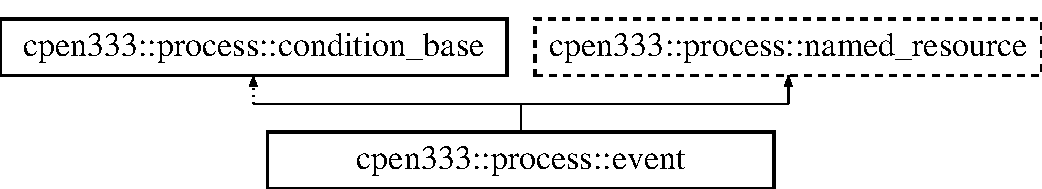
\includegraphics[height=2.000000cm]{classcpen333_1_1process_1_1event}
\end{center}
\end{figure}
\subsection*{Public Member Functions}
\begin{DoxyCompactItemize}
\item 
\hyperlink{classcpen333_1_1process_1_1event_a83253320779b5b9fd26b823608e69977}{event} (const std\+::string \&name)
\begin{DoxyCompactList}\small\item\em Creates or connects to a named event. \end{DoxyCompactList}\item 
void \hyperlink{classcpen333_1_1process_1_1event_ae02584676aa834eef81b74d01ceb3ea5}{wait} ()
\begin{DoxyCompactList}\small\item\em Waits for the event to be triggered. \end{DoxyCompactList}\item 
{\footnotesize template$<$class Rep , class Period $>$ }\\bool \hyperlink{classcpen333_1_1process_1_1event_a9b887906af309ccc8687cb91f3c66b25}{wait\+\_\+for} (const std\+::chrono\+::duration$<$ Rep, Period $>$ \&rel\+\_\+time)
\begin{DoxyCompactList}\small\item\em Waits for the event to be triggered or for a timeout period to elapse. \end{DoxyCompactList}\item 
{\footnotesize template$<$class Clock , class Duration $>$ }\\bool \hyperlink{classcpen333_1_1process_1_1event_ac64e2c2152ce879b199271f96e0a7335}{wait\+\_\+until} (const std\+::chrono\+::time\+\_\+point$<$ Clock, Duration $>$ \&timeout\+\_\+time)
\begin{DoxyCompactList}\small\item\em Waits for the event to be triggered or for a time-\/point to be reached. \end{DoxyCompactList}\item 
void \hyperlink{classcpen333_1_1process_1_1event_a47077325cc6cb29df3aba00de683ce42}{notify\+\_\+one} ()
\begin{DoxyCompactList}\small\item\em Wake a single thread waiting for the event to be triggered. \end{DoxyCompactList}\item 
void \hyperlink{classcpen333_1_1process_1_1event_a80184c9e2762fb1a0d7f3a9ff6ae27e7}{notify\+\_\+all} ()
\begin{DoxyCompactList}\small\item\em Wake all threads waiting for the event to be triggered. \end{DoxyCompactList}\item 
virtual bool \hyperlink{classcpen333_1_1process_1_1event_a37a2d53cbf4a90da6b4dbd5853f23b32}{unlink} ()
\begin{DoxyCompactList}\small\item\em Detaches the name from the named resource. \end{DoxyCompactList}\end{DoxyCompactItemize}
\subsection*{Static Public Member Functions}
\begin{DoxyCompactItemize}
\item 
static bool \hyperlink{classcpen333_1_1process_1_1event_a5e013471e78e37c47036bd408987662a}{unlink} (const std\+::string \&name)
\begin{DoxyCompactList}\small\item\em Unlinks the name without needing to create a resource. \end{DoxyCompactList}\end{DoxyCompactItemize}


\subsection{Detailed Description}
Event primitive, acting like a turnstile. 

A named synchronization primitive that allows multiple threads and processes to wait until the event is notified. The notifier can either {\ttfamily \hyperlink{classcpen333_1_1process_1_1event_a47077325cc6cb29df3aba00de683ce42}{notify\+\_\+one()}} to let a single waiter through (if any), or {\ttfamily \hyperlink{classcpen333_1_1process_1_1event_a80184c9e2762fb1a0d7f3a9ff6ae27e7}{notify\+\_\+all()}} to let everyone currently waiting through. 

\subsection{Constructor \& Destructor Documentation}
\mbox{\Hypertarget{classcpen333_1_1process_1_1event_a83253320779b5b9fd26b823608e69977}\label{classcpen333_1_1process_1_1event_a83253320779b5b9fd26b823608e69977}} 
\index{cpen333\+::process\+::event@{cpen333\+::process\+::event}!event@{event}}
\index{event@{event}!cpen333\+::process\+::event@{cpen333\+::process\+::event}}
\subsubsection{\texorpdfstring{event()}{event()}}
{\footnotesize\ttfamily cpen333\+::process\+::event\+::event (\begin{DoxyParamCaption}\item[{const std\+::string \&}]{name }\end{DoxyParamCaption})\hspace{0.3cm}{\ttfamily [inline]}}



Creates or connects to a named event. 


\begin{DoxyParams}{Parameters}
{\em name} & name identifier for creating or connecting to an existing inter-\/process event \\
\hline
\end{DoxyParams}


\subsection{Member Function Documentation}
\mbox{\Hypertarget{classcpen333_1_1process_1_1event_a80184c9e2762fb1a0d7f3a9ff6ae27e7}\label{classcpen333_1_1process_1_1event_a80184c9e2762fb1a0d7f3a9ff6ae27e7}} 
\index{cpen333\+::process\+::event@{cpen333\+::process\+::event}!notify\+\_\+all@{notify\+\_\+all}}
\index{notify\+\_\+all@{notify\+\_\+all}!cpen333\+::process\+::event@{cpen333\+::process\+::event}}
\subsubsection{\texorpdfstring{notify\+\_\+all()}{notify\_all()}}
{\footnotesize\ttfamily void cpen333\+::process\+::event\+::notify\+\_\+all (\begin{DoxyParamCaption}{ }\end{DoxyParamCaption})\hspace{0.3cm}{\ttfamily [inline]}}



Wake all threads waiting for the event to be triggered. 

All threads waiting for the event will be awoken and will continue. \mbox{\Hypertarget{classcpen333_1_1process_1_1event_a47077325cc6cb29df3aba00de683ce42}\label{classcpen333_1_1process_1_1event_a47077325cc6cb29df3aba00de683ce42}} 
\index{cpen333\+::process\+::event@{cpen333\+::process\+::event}!notify\+\_\+one@{notify\+\_\+one}}
\index{notify\+\_\+one@{notify\+\_\+one}!cpen333\+::process\+::event@{cpen333\+::process\+::event}}
\subsubsection{\texorpdfstring{notify\+\_\+one()}{notify\_one()}}
{\footnotesize\ttfamily void cpen333\+::process\+::event\+::notify\+\_\+one (\begin{DoxyParamCaption}{ }\end{DoxyParamCaption})\hspace{0.3cm}{\ttfamily [inline]}}



Wake a single thread waiting for the event to be triggered. 

Note that the choice of thread to be awoken is up to the underlying system. Threads are not necessarily notified in order of arrival. \mbox{\Hypertarget{classcpen333_1_1process_1_1event_a37a2d53cbf4a90da6b4dbd5853f23b32}\label{classcpen333_1_1process_1_1event_a37a2d53cbf4a90da6b4dbd5853f23b32}} 
\index{cpen333\+::process\+::event@{cpen333\+::process\+::event}!unlink@{unlink}}
\index{unlink@{unlink}!cpen333\+::process\+::event@{cpen333\+::process\+::event}}
\subsubsection{\texorpdfstring{unlink()}{unlink()}\hspace{0.1cm}{\footnotesize\ttfamily [1/2]}}
{\footnotesize\ttfamily virtual bool cpen333\+::process\+::event\+::unlink (\begin{DoxyParamCaption}{ }\end{DoxyParamCaption})\hspace{0.3cm}{\ttfamily [inline]}, {\ttfamily [virtual]}}



Detaches the name from the named resource. 

On P\+O\+S\+IX systems, named resources will persist beyond the lifetime of any process that uses them as long as the name has not been unlinked (or until the system is rebooted). Calling {\ttfamily unlink} will detach the name, allowing the resource to be freed once all current users have exited.

\begin{DoxyReturn}{Returns}
{\ttfamily true} if unlink is successful, {\ttfamily false} if unlinking is not supported or if an error has occurred. 
\end{DoxyReturn}


Reimplemented from \hyperlink{classcpen333_1_1process_1_1condition__base_acd6d0b53a828aa161ccad06885eaa15c}{cpen333\+::process\+::condition\+\_\+base}.

\mbox{\Hypertarget{classcpen333_1_1process_1_1event_a5e013471e78e37c47036bd408987662a}\label{classcpen333_1_1process_1_1event_a5e013471e78e37c47036bd408987662a}} 
\index{cpen333\+::process\+::event@{cpen333\+::process\+::event}!unlink@{unlink}}
\index{unlink@{unlink}!cpen333\+::process\+::event@{cpen333\+::process\+::event}}
\subsubsection{\texorpdfstring{unlink()}{unlink()}\hspace{0.1cm}{\footnotesize\ttfamily [2/2]}}
{\footnotesize\ttfamily static bool cpen333\+::process\+::event\+::unlink (\begin{DoxyParamCaption}\item[{const std\+::string \&}]{name }\end{DoxyParamCaption})\hspace{0.3cm}{\ttfamily [inline]}, {\ttfamily [static]}}



Unlinks the name without needing to create a resource. 

Implementers should also provide a static method for unlinking. The purpose is mainly for clean-\/up of existing resources.


\begin{DoxyParams}{Parameters}
{\em name} & desired resource name \\
\hline
\end{DoxyParams}
\begin{DoxyReturn}{Returns}
{\ttfamily true} if unlink successful, {\ttfamily false} if not successful or not supported 
\end{DoxyReturn}
\mbox{\Hypertarget{classcpen333_1_1process_1_1event_ae02584676aa834eef81b74d01ceb3ea5}\label{classcpen333_1_1process_1_1event_ae02584676aa834eef81b74d01ceb3ea5}} 
\index{cpen333\+::process\+::event@{cpen333\+::process\+::event}!wait@{wait}}
\index{wait@{wait}!cpen333\+::process\+::event@{cpen333\+::process\+::event}}
\subsubsection{\texorpdfstring{wait()}{wait()}}
{\footnotesize\ttfamily void cpen333\+::process\+::event\+::wait (\begin{DoxyParamCaption}{ }\end{DoxyParamCaption})\hspace{0.3cm}{\ttfamily [inline]}}



Waits for the event to be triggered. 

Causes the current thread to block until either {\ttfamily \hyperlink{classcpen333_1_1process_1_1event_a80184c9e2762fb1a0d7f3a9ff6ae27e7}{notify\+\_\+all()}} is called, or {\ttfamily \hyperlink{classcpen333_1_1process_1_1event_a47077325cc6cb29df3aba00de683ce42}{notify\+\_\+one()}} and this thread happens to be the one awoken. Note that order of wakes is system-\/dependent, and not necessarily in order of arrival. This event will {\itshape not} exhibit spurious wake-\/ups. A thread will be forced to wait here indefinitely until the event is triggered. \mbox{\Hypertarget{classcpen333_1_1process_1_1event_a9b887906af309ccc8687cb91f3c66b25}\label{classcpen333_1_1process_1_1event_a9b887906af309ccc8687cb91f3c66b25}} 
\index{cpen333\+::process\+::event@{cpen333\+::process\+::event}!wait\+\_\+for@{wait\+\_\+for}}
\index{wait\+\_\+for@{wait\+\_\+for}!cpen333\+::process\+::event@{cpen333\+::process\+::event}}
\subsubsection{\texorpdfstring{wait\+\_\+for()}{wait\_for()}}
{\footnotesize\ttfamily template$<$class Rep , class Period $>$ \\
bool cpen333\+::process\+::event\+::wait\+\_\+for (\begin{DoxyParamCaption}\item[{const std\+::chrono\+::duration$<$ Rep, Period $>$ \&}]{rel\+\_\+time }\end{DoxyParamCaption})\hspace{0.3cm}{\ttfamily [inline]}}



Waits for the event to be triggered or for a timeout period to elapse. 

Causes the current thread to block until {\ttfamily \hyperlink{classcpen333_1_1process_1_1event_a80184c9e2762fb1a0d7f3a9ff6ae27e7}{notify\+\_\+all()}} is called, or {\ttfamily \hyperlink{classcpen333_1_1process_1_1event_a47077325cc6cb29df3aba00de683ce42}{notify\+\_\+one()}} and this thread happens to be the one awoken, or until the specified timeout period elapses, whichever comes first. 
\begin{DoxyTemplParams}{Template Parameters}
{\em Rep} & timeout duration representation \\
\hline
{\em Period} & timeout clock period \\
\hline
\end{DoxyTemplParams}

\begin{DoxyParams}{Parameters}
{\em rel\+\_\+time} & maximum relative time to wait for condition to be set \\
\hline
\end{DoxyParams}
\begin{DoxyReturn}{Returns}
{\ttfamily true} if event is triggered, {\ttfamily false} if timeout has elapsed without event being triggered 
\end{DoxyReturn}
\mbox{\Hypertarget{classcpen333_1_1process_1_1event_ac64e2c2152ce879b199271f96e0a7335}\label{classcpen333_1_1process_1_1event_ac64e2c2152ce879b199271f96e0a7335}} 
\index{cpen333\+::process\+::event@{cpen333\+::process\+::event}!wait\+\_\+until@{wait\+\_\+until}}
\index{wait\+\_\+until@{wait\+\_\+until}!cpen333\+::process\+::event@{cpen333\+::process\+::event}}
\subsubsection{\texorpdfstring{wait\+\_\+until()}{wait\_until()}}
{\footnotesize\ttfamily template$<$class Clock , class Duration $>$ \\
bool cpen333\+::process\+::event\+::wait\+\_\+until (\begin{DoxyParamCaption}\item[{const std\+::chrono\+::time\+\_\+point$<$ Clock, Duration $>$ \&}]{timeout\+\_\+time }\end{DoxyParamCaption})\hspace{0.3cm}{\ttfamily [inline]}}



Waits for the event to be triggered or for a time-\/point to be reached. 

Causes the current thread to block until {\ttfamily \hyperlink{classcpen333_1_1process_1_1event_a80184c9e2762fb1a0d7f3a9ff6ae27e7}{notify\+\_\+all()}} is called, or {\ttfamily \hyperlink{classcpen333_1_1process_1_1event_a47077325cc6cb29df3aba00de683ce42}{notify\+\_\+one()}} and this thread happens to be the one awoken, or until the specified timeout time has been reached, whichever comes first.


\begin{DoxyTemplParams}{Template Parameters}
{\em Clock} & clock type \\
\hline
{\em Duration} & clock duration type \\
\hline
\end{DoxyTemplParams}

\begin{DoxyParams}{Parameters}
{\em timeout\+\_\+time} & absolute timeout time \\
\hline
\end{DoxyParams}
\begin{DoxyReturn}{Returns}
{\ttfamily true} if event is triggered, {\ttfamily false} if timeout time has been reached without event 
\end{DoxyReturn}


The documentation for this class was generated from the following file\+:\begin{DoxyCompactItemize}
\item 
D\+:/school/teaching/\+C\+P\+E\+N333/workspace/labs/include/cpen333/process/\hyperlink{process_2event_8h}{event.\+h}\end{DoxyCompactItemize}

\hypertarget{classcpen333_1_1process_1_1fifo}{}\section{cpen333\+:\+:process\+:\+:fifo$<$ Value\+Type $>$ Class Template Reference}
\label{classcpen333_1_1process_1_1fifo}\index{cpen333\+::process\+::fifo$<$ Value\+Type $>$@{cpen333\+::process\+::fifo$<$ Value\+Type $>$}}


Simple thread-\/safe multi-\/process first-\/in-\/first-\/out queue using a circular buffer.  




{\ttfamily \#include $<$fifo.\+h$>$}

Inheritance diagram for cpen333\+:\+:process\+:\+:fifo$<$ Value\+Type $>$\+:\begin{figure}[H]
\begin{center}
\leavevmode
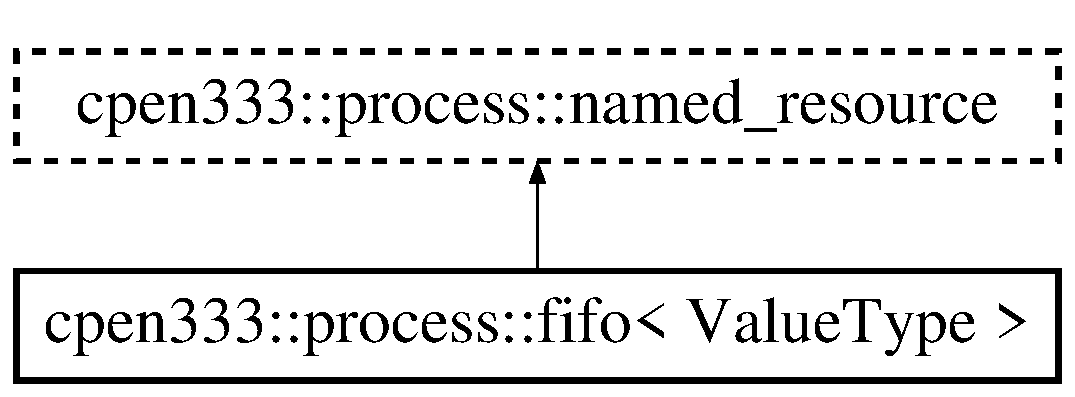
\includegraphics[height=2.000000cm]{classcpen333_1_1process_1_1fifo}
\end{center}
\end{figure}
\subsection*{Public Types}
\begin{DoxyCompactItemize}
\item 
\mbox{\Hypertarget{classcpen333_1_1process_1_1fifo_abc26c9f811226c81d390bd32dd4a3a53}\label{classcpen333_1_1process_1_1fifo_abc26c9f811226c81d390bd32dd4a3a53}} 
typedef Value\+Type \hyperlink{classcpen333_1_1process_1_1fifo_abc26c9f811226c81d390bd32dd4a3a53}{value\+\_\+type}
\begin{DoxyCompactList}\small\item\em data type stored in buffer \end{DoxyCompactList}\end{DoxyCompactItemize}
\subsection*{Public Member Functions}
\begin{DoxyCompactItemize}
\item 
\hyperlink{classcpen333_1_1process_1_1fifo_abbac3b7b35974927626c0fc96540a5c9}{fifo} (const std\+::string \&name, size\+\_\+t \hyperlink{classcpen333_1_1process_1_1fifo_aeaf7bd6333245fad222fcf088e589ad6}{size}=1024)
\begin{DoxyCompactList}\small\item\em Creates or connects to an existing named fifo. \end{DoxyCompactList}\item 
void \hyperlink{classcpen333_1_1process_1_1fifo_a169331a45d9b30c6303ab8300b7901e8}{push} (const Value\+Type \&val)
\begin{DoxyCompactList}\small\item\em Add a item to the fifo. \end{DoxyCompactList}\item 
bool \hyperlink{classcpen333_1_1process_1_1fifo_ad6a7fb652df17c022023fcc805ba61eb}{try\+\_\+push} (const Value\+Type \&val)
\begin{DoxyCompactList}\small\item\em Tries to add an item to the fifo without blocking. \end{DoxyCompactList}\item 
{\footnotesize template$<$typename Rep , typename Period $>$ }\\bool \hyperlink{classcpen333_1_1process_1_1fifo_a2904c1ed9d23f0d7fd034216c5509688}{try\+\_\+push\+\_\+for} (const Value\+Type \&val, std\+::chrono\+::duration$<$ Rep, Period $>$ \&rel\+\_\+time)
\begin{DoxyCompactList}\small\item\em Tries to add an item to the fifo, will wait for a maximum amount of time before aborting. \end{DoxyCompactList}\item 
{\footnotesize template$<$typename Clock , typename Duration $>$ }\\bool \hyperlink{classcpen333_1_1process_1_1fifo_abe9fee85225689f4104f263510814db0}{try\+\_\+push\+\_\+until} (const Value\+Type \&val, const std\+::chrono\+::time\+\_\+point$<$ Clock, Duration $>$ \&timeout)
\begin{DoxyCompactList}\small\item\em Tries to add an item to the fifo, will wait until a timeout time is reached before aborting. \end{DoxyCompactList}\item 
void \hyperlink{classcpen333_1_1process_1_1fifo_af29e5bd6d8b0fe551c4d7532ffcb331e}{pop} (Value\+Type $\ast$out)
\begin{DoxyCompactList}\small\item\em Removes the next item in the fifo. \end{DoxyCompactList}\item 
Value\+Type \hyperlink{classcpen333_1_1process_1_1fifo_a40796c0eb39299ff4f8c49a789268386}{pop} ()
\begin{DoxyCompactList}\small\item\em Removes and returns the next item in the fifo. \end{DoxyCompactList}\item 
bool \hyperlink{classcpen333_1_1process_1_1fifo_a6f3e1f84d8a72e620f44bc5c018b3a9c}{try\+\_\+pop} (Value\+Type $\ast$out)
\begin{DoxyCompactList}\small\item\em Tries to remove and return the next item in the fifo without blocking. \end{DoxyCompactList}\item 
{\footnotesize template$<$typename Rep , typename Period $>$ }\\bool \hyperlink{classcpen333_1_1process_1_1fifo_a6411f9f377c2be43500bc53883651120}{try\+\_\+pop\+\_\+for} (Value\+Type $\ast$out, std\+::chrono\+::duration$<$ Rep, Period $>$ \&rel\+\_\+time)
\begin{DoxyCompactList}\small\item\em Tries to remove an item from the fifo, will wait for a maximum amount of time before aborting. \end{DoxyCompactList}\item 
{\footnotesize template$<$typename Clock , typename Duration $>$ }\\bool \hyperlink{classcpen333_1_1process_1_1fifo_a7e66a7f6e91c0725ad6a5f3940668e64}{try\+\_\+pop\+\_\+until} (Value\+Type $\ast$out, const std\+::chrono\+::time\+\_\+point$<$ Clock, Duration $>$ \&timeout)
\begin{DoxyCompactList}\small\item\em Tries to remove an item from the fifo, will wait for a maximum timeout time to be reached before aborting. \end{DoxyCompactList}\item 
void \hyperlink{classcpen333_1_1process_1_1fifo_ac501e62c2253097f89d713558d888d16}{peek} (Value\+Type $\ast$out)
\begin{DoxyCompactList}\small\item\em Peeks at the next item in the fifo without removing it. \end{DoxyCompactList}\item 
Value\+Type \hyperlink{classcpen333_1_1process_1_1fifo_a785266ee082e1917198bd0d701b25e50}{peek} ()
\begin{DoxyCompactList}\small\item\em Peeks at the next item in the fifo without removing it. \end{DoxyCompactList}\item 
bool \hyperlink{classcpen333_1_1process_1_1fifo_a0518230659a2ec8568f05377f4e2e727}{try\+\_\+peek} (Value\+Type $\ast$out)
\begin{DoxyCompactList}\small\item\em Tries to peek at the next item in the fifo without blocking. \end{DoxyCompactList}\item 
{\footnotesize template$<$typename Rep , typename Period $>$ }\\bool \hyperlink{classcpen333_1_1process_1_1fifo_a61d351911485a6cef80404da4aa663ec}{try\+\_\+peek\+\_\+for} (Value\+Type $\ast$out, std\+::chrono\+::duration$<$ Rep, Period $>$ \&rel\+\_\+time)
\begin{DoxyCompactList}\small\item\em Tries to peek at the next item in the fifo, will wait for a maximum amount of time before aborting. \end{DoxyCompactList}\item 
{\footnotesize template$<$typename Clock , typename Duration $>$ }\\bool \hyperlink{classcpen333_1_1process_1_1fifo_ac587ec4df8ae29b25a3e21ac7114e335}{try\+\_\+peek\+\_\+until} (Value\+Type $\ast$out, const std\+::chrono\+::time\+\_\+point$<$ Clock, Duration $>$ \&timeout)
\begin{DoxyCompactList}\small\item\em Tries to peek at the next item in the fifo, will wait for a maximum timeout time before aborting. \end{DoxyCompactList}\item 
size\+\_\+t \hyperlink{classcpen333_1_1process_1_1fifo_aeaf7bd6333245fad222fcf088e589ad6}{size} ()
\begin{DoxyCompactList}\small\item\em Number of items currently in the fifo. \end{DoxyCompactList}\item 
bool \hyperlink{classcpen333_1_1process_1_1fifo_ae2ce36a0885d0c3ded0997ec2586aabe}{empty} ()
\begin{DoxyCompactList}\small\item\em Check if fifo queue is currently empty. \end{DoxyCompactList}\item 
bool \hyperlink{classcpen333_1_1process_1_1fifo_a85f9c252de8044d57568e99b64cbb860}{unlink} ()
\begin{DoxyCompactList}\small\item\em Detaches the name from the named resource. \end{DoxyCompactList}\end{DoxyCompactItemize}
\subsection*{Static Public Member Functions}
\begin{DoxyCompactItemize}
\item 
static bool \hyperlink{classcpen333_1_1process_1_1fifo_a893a14908a88de202fe2804dd890f958}{unlink} (const std\+::string \&name)
\begin{DoxyCompactList}\small\item\em Unlinks the name without needing to create a resource. \end{DoxyCompactList}\end{DoxyCompactItemize}


\subsection{Detailed Description}
\subsubsection*{template$<$typename Value\+Type$>$\newline
class cpen333\+::process\+::fifo$<$ Value\+Type $>$}

Simple thread-\/safe multi-\/process first-\/in-\/first-\/out queue using a circular buffer. 

The buffer can only contain a single type of object. Push will block until space is available in the queue. Pop will block until there is an item in the queue. 
\begin{DoxyTemplParams}{Template Parameters}
{\em Value\+Type} & type of data to store in the queue \\
\hline
\end{DoxyTemplParams}


\subsection{Constructor \& Destructor Documentation}
\mbox{\Hypertarget{classcpen333_1_1process_1_1fifo_abbac3b7b35974927626c0fc96540a5c9}\label{classcpen333_1_1process_1_1fifo_abbac3b7b35974927626c0fc96540a5c9}} 
\index{cpen333\+::process\+::fifo@{cpen333\+::process\+::fifo}!fifo@{fifo}}
\index{fifo@{fifo}!cpen333\+::process\+::fifo@{cpen333\+::process\+::fifo}}
\subsubsection{\texorpdfstring{fifo()}{fifo()}}
{\footnotesize\ttfamily template$<$typename Value\+Type$>$ \\
\hyperlink{classcpen333_1_1process_1_1fifo}{cpen333\+::process\+::fifo}$<$ Value\+Type $>$\+::\hyperlink{classcpen333_1_1process_1_1fifo}{fifo} (\begin{DoxyParamCaption}\item[{const std\+::string \&}]{name,  }\item[{size\+\_\+t}]{size = {\ttfamily 1024} }\end{DoxyParamCaption})\hspace{0.3cm}{\ttfamily [inline]}}



Creates or connects to an existing named fifo. 


\begin{DoxyParams}{Parameters}
{\em name} & name identifier for creating or connecting to an existing inter-\/process fifo \\
\hline
{\em size} & if creating, the maximum number of elements that can be stored in the queue without blocking \\
\hline
\end{DoxyParams}


\subsection{Member Function Documentation}
\mbox{\Hypertarget{classcpen333_1_1process_1_1fifo_ae2ce36a0885d0c3ded0997ec2586aabe}\label{classcpen333_1_1process_1_1fifo_ae2ce36a0885d0c3ded0997ec2586aabe}} 
\index{cpen333\+::process\+::fifo@{cpen333\+::process\+::fifo}!empty@{empty}}
\index{empty@{empty}!cpen333\+::process\+::fifo@{cpen333\+::process\+::fifo}}
\subsubsection{\texorpdfstring{empty()}{empty()}}
{\footnotesize\ttfamily template$<$typename Value\+Type$>$ \\
bool \hyperlink{classcpen333_1_1process_1_1fifo}{cpen333\+::process\+::fifo}$<$ Value\+Type $>$\+::empty (\begin{DoxyParamCaption}{ }\end{DoxyParamCaption})\hspace{0.3cm}{\ttfamily [inline]}}



Check if fifo queue is currently empty. 

This method should be used sparingly, since items could be added/removed during or immediately after the call, making the result potentially unreliable

\begin{DoxyReturn}{Returns}
{\ttfamily true} if empty, {\ttfamily false} otherwise 
\end{DoxyReturn}
\mbox{\Hypertarget{classcpen333_1_1process_1_1fifo_ac501e62c2253097f89d713558d888d16}\label{classcpen333_1_1process_1_1fifo_ac501e62c2253097f89d713558d888d16}} 
\index{cpen333\+::process\+::fifo@{cpen333\+::process\+::fifo}!peek@{peek}}
\index{peek@{peek}!cpen333\+::process\+::fifo@{cpen333\+::process\+::fifo}}
\subsubsection{\texorpdfstring{peek()}{peek()}\hspace{0.1cm}{\footnotesize\ttfamily [1/2]}}
{\footnotesize\ttfamily template$<$typename Value\+Type$>$ \\
void \hyperlink{classcpen333_1_1process_1_1fifo}{cpen333\+::process\+::fifo}$<$ Value\+Type $>$\+::peek (\begin{DoxyParamCaption}\item[{Value\+Type $\ast$}]{out }\end{DoxyParamCaption})\hspace{0.3cm}{\ttfamily [inline]}}



Peeks at the next item in the fifo without removing it. 

Populates memory pointed to by {\ttfamily out} with next item in fifo. If there are currently no items, this method will block until an item becomes available. The item will remain in the fifo for the next {\ttfamily peek} or {\ttfamily pop} operation.


\begin{DoxyParams}{Parameters}
{\em out} & destination. If {\ttfamily nullptr}, nothing happens. \\
\hline
\end{DoxyParams}
\mbox{\Hypertarget{classcpen333_1_1process_1_1fifo_a785266ee082e1917198bd0d701b25e50}\label{classcpen333_1_1process_1_1fifo_a785266ee082e1917198bd0d701b25e50}} 
\index{cpen333\+::process\+::fifo@{cpen333\+::process\+::fifo}!peek@{peek}}
\index{peek@{peek}!cpen333\+::process\+::fifo@{cpen333\+::process\+::fifo}}
\subsubsection{\texorpdfstring{peek()}{peek()}\hspace{0.1cm}{\footnotesize\ttfamily [2/2]}}
{\footnotesize\ttfamily template$<$typename Value\+Type$>$ \\
Value\+Type \hyperlink{classcpen333_1_1process_1_1fifo}{cpen333\+::process\+::fifo}$<$ Value\+Type $>$\+::peek (\begin{DoxyParamCaption}{ }\end{DoxyParamCaption})\hspace{0.3cm}{\ttfamily [inline]}}



Peeks at the next item in the fifo without removing it. 

Returns the next item in the fifo. If there are currently no items, this method will block until one becomes available. The item will remain in the fifo for the next {\ttfamily peek} or {\ttfamily pop} operation.

\begin{DoxyReturn}{Returns}
next item in the fifo. 
\end{DoxyReturn}
\mbox{\Hypertarget{classcpen333_1_1process_1_1fifo_af29e5bd6d8b0fe551c4d7532ffcb331e}\label{classcpen333_1_1process_1_1fifo_af29e5bd6d8b0fe551c4d7532ffcb331e}} 
\index{cpen333\+::process\+::fifo@{cpen333\+::process\+::fifo}!pop@{pop}}
\index{pop@{pop}!cpen333\+::process\+::fifo@{cpen333\+::process\+::fifo}}
\subsubsection{\texorpdfstring{pop()}{pop()}\hspace{0.1cm}{\footnotesize\ttfamily [1/2]}}
{\footnotesize\ttfamily template$<$typename Value\+Type$>$ \\
void \hyperlink{classcpen333_1_1process_1_1fifo}{cpen333\+::process\+::fifo}$<$ Value\+Type $>$\+::pop (\begin{DoxyParamCaption}\item[{Value\+Type $\ast$}]{out }\end{DoxyParamCaption})\hspace{0.3cm}{\ttfamily [inline]}}



Removes the next item in the fifo. 

Populates memory pointed to by {\ttfamily out} with next item in the fifo. If there are no items in the fifo, then this will block until one is available.


\begin{DoxyParams}{Parameters}
{\em out} & destination. If {\ttfamily nullptr}, item is removed but not returned. \\
\hline
\end{DoxyParams}
\mbox{\Hypertarget{classcpen333_1_1process_1_1fifo_a40796c0eb39299ff4f8c49a789268386}\label{classcpen333_1_1process_1_1fifo_a40796c0eb39299ff4f8c49a789268386}} 
\index{cpen333\+::process\+::fifo@{cpen333\+::process\+::fifo}!pop@{pop}}
\index{pop@{pop}!cpen333\+::process\+::fifo@{cpen333\+::process\+::fifo}}
\subsubsection{\texorpdfstring{pop()}{pop()}\hspace{0.1cm}{\footnotesize\ttfamily [2/2]}}
{\footnotesize\ttfamily template$<$typename Value\+Type$>$ \\
Value\+Type \hyperlink{classcpen333_1_1process_1_1fifo}{cpen333\+::process\+::fifo}$<$ Value\+Type $>$\+::pop (\begin{DoxyParamCaption}{ }\end{DoxyParamCaption})\hspace{0.3cm}{\ttfamily [inline]}}



Removes and returns the next item in the fifo. 

If there are no items in the fifo, then this will block until one is available.

\begin{DoxyReturn}{Returns}
next item in the fifo 
\end{DoxyReturn}
\mbox{\Hypertarget{classcpen333_1_1process_1_1fifo_a169331a45d9b30c6303ab8300b7901e8}\label{classcpen333_1_1process_1_1fifo_a169331a45d9b30c6303ab8300b7901e8}} 
\index{cpen333\+::process\+::fifo@{cpen333\+::process\+::fifo}!push@{push}}
\index{push@{push}!cpen333\+::process\+::fifo@{cpen333\+::process\+::fifo}}
\subsubsection{\texorpdfstring{push()}{push()}}
{\footnotesize\ttfamily template$<$typename Value\+Type$>$ \\
void \hyperlink{classcpen333_1_1process_1_1fifo}{cpen333\+::process\+::fifo}$<$ Value\+Type $>$\+::push (\begin{DoxyParamCaption}\item[{const Value\+Type \&}]{val }\end{DoxyParamCaption})\hspace{0.3cm}{\ttfamily [inline]}}



Add a item to the fifo. 


\begin{DoxyParams}{Parameters}
{\em val} & value to add \\
\hline
\end{DoxyParams}
\mbox{\Hypertarget{classcpen333_1_1process_1_1fifo_aeaf7bd6333245fad222fcf088e589ad6}\label{classcpen333_1_1process_1_1fifo_aeaf7bd6333245fad222fcf088e589ad6}} 
\index{cpen333\+::process\+::fifo@{cpen333\+::process\+::fifo}!size@{size}}
\index{size@{size}!cpen333\+::process\+::fifo@{cpen333\+::process\+::fifo}}
\subsubsection{\texorpdfstring{size()}{size()}}
{\footnotesize\ttfamily template$<$typename Value\+Type$>$ \\
size\+\_\+t \hyperlink{classcpen333_1_1process_1_1fifo}{cpen333\+::process\+::fifo}$<$ Value\+Type $>$\+::size (\begin{DoxyParamCaption}{ }\end{DoxyParamCaption})\hspace{0.3cm}{\ttfamily [inline]}}



Number of items currently in the fifo. 

This method should be used sparingly, since items could be added/removed during or immediately after the call, making the result potentially unreliable.

\begin{DoxyReturn}{Returns}
number of items 
\end{DoxyReturn}
\mbox{\Hypertarget{classcpen333_1_1process_1_1fifo_a0518230659a2ec8568f05377f4e2e727}\label{classcpen333_1_1process_1_1fifo_a0518230659a2ec8568f05377f4e2e727}} 
\index{cpen333\+::process\+::fifo@{cpen333\+::process\+::fifo}!try\+\_\+peek@{try\+\_\+peek}}
\index{try\+\_\+peek@{try\+\_\+peek}!cpen333\+::process\+::fifo@{cpen333\+::process\+::fifo}}
\subsubsection{\texorpdfstring{try\+\_\+peek()}{try\_peek()}}
{\footnotesize\ttfamily template$<$typename Value\+Type$>$ \\
bool \hyperlink{classcpen333_1_1process_1_1fifo}{cpen333\+::process\+::fifo}$<$ Value\+Type $>$\+::try\+\_\+peek (\begin{DoxyParamCaption}\item[{Value\+Type $\ast$}]{out }\end{DoxyParamCaption})\hspace{0.3cm}{\ttfamily [inline]}}



Tries to peek at the next item in the fifo without blocking. 

Populates memory pointed to by {\ttfamily out} with the next item in the fifo. If there are no items, then this will return immediately without peeking at the item. The item will remain in the fifo for the next {\ttfamily peek} or {\ttfamily pop} operation.


\begin{DoxyParams}{Parameters}
{\em out} & destination. If {\ttfamily nullptr}, nothing happens. \\
\hline
\end{DoxyParams}
\begin{DoxyReturn}{Returns}
{\ttfamily true} if item was successfully peeked, {\ttfamily false} otherwise 
\end{DoxyReturn}
\mbox{\Hypertarget{classcpen333_1_1process_1_1fifo_a61d351911485a6cef80404da4aa663ec}\label{classcpen333_1_1process_1_1fifo_a61d351911485a6cef80404da4aa663ec}} 
\index{cpen333\+::process\+::fifo@{cpen333\+::process\+::fifo}!try\+\_\+peek\+\_\+for@{try\+\_\+peek\+\_\+for}}
\index{try\+\_\+peek\+\_\+for@{try\+\_\+peek\+\_\+for}!cpen333\+::process\+::fifo@{cpen333\+::process\+::fifo}}
\subsubsection{\texorpdfstring{try\+\_\+peek\+\_\+for()}{try\_peek\_for()}}
{\footnotesize\ttfamily template$<$typename Value\+Type$>$ \\
template$<$typename Rep , typename Period $>$ \\
bool \hyperlink{classcpen333_1_1process_1_1fifo}{cpen333\+::process\+::fifo}$<$ Value\+Type $>$\+::try\+\_\+peek\+\_\+for (\begin{DoxyParamCaption}\item[{Value\+Type $\ast$}]{out,  }\item[{std\+::chrono\+::duration$<$ Rep, Period $>$ \&}]{rel\+\_\+time }\end{DoxyParamCaption})\hspace{0.3cm}{\ttfamily [inline]}}



Tries to peek at the next item in the fifo, will wait for a maximum amount of time before aborting. 

If it is not possible to peek at an item in the fifo immediately, then the current thread will block until either an item becomes available, or a timeout period has elapsed. The item will remain in the fifo for the next {\ttfamily peek} or {\ttfamily pop} operation.


\begin{DoxyTemplParams}{Template Parameters}
{\em Rep} & duration representation \\
\hline
{\em Period} & duration period \\
\hline
\end{DoxyTemplParams}

\begin{DoxyParams}{Parameters}
{\em out} & destination. If {\ttfamily nullptr}, nothing happens \\
\hline
{\em rel\+\_\+time} & relative timeout time \\
\hline
\end{DoxyParams}
\begin{DoxyReturn}{Returns}
{\ttfamily true} if item successfully peeked, {\ttfamily false} if timeout elapsed 
\end{DoxyReturn}
\mbox{\Hypertarget{classcpen333_1_1process_1_1fifo_ac587ec4df8ae29b25a3e21ac7114e335}\label{classcpen333_1_1process_1_1fifo_ac587ec4df8ae29b25a3e21ac7114e335}} 
\index{cpen333\+::process\+::fifo@{cpen333\+::process\+::fifo}!try\+\_\+peek\+\_\+until@{try\+\_\+peek\+\_\+until}}
\index{try\+\_\+peek\+\_\+until@{try\+\_\+peek\+\_\+until}!cpen333\+::process\+::fifo@{cpen333\+::process\+::fifo}}
\subsubsection{\texorpdfstring{try\+\_\+peek\+\_\+until()}{try\_peek\_until()}}
{\footnotesize\ttfamily template$<$typename Value\+Type$>$ \\
template$<$typename Clock , typename Duration $>$ \\
bool \hyperlink{classcpen333_1_1process_1_1fifo}{cpen333\+::process\+::fifo}$<$ Value\+Type $>$\+::try\+\_\+peek\+\_\+until (\begin{DoxyParamCaption}\item[{Value\+Type $\ast$}]{out,  }\item[{const std\+::chrono\+::time\+\_\+point$<$ Clock, Duration $>$ \&}]{timeout }\end{DoxyParamCaption})\hspace{0.3cm}{\ttfamily [inline]}}



Tries to peek at the next item in the fifo, will wait for a maximum timeout time before aborting. 

If it is not possible to peek at the next item in the fifo immediately, then the current thread will block until either an item becomes available, or a timeout time has been reached. The item will remain in the fifo for the next {\ttfamily peek} or {\ttfamily pop} operation.


\begin{DoxyTemplParams}{Template Parameters}
{\em Clock} & clock type \\
\hline
{\em Duration} & clock duration type \\
\hline
\end{DoxyTemplParams}

\begin{DoxyParams}{Parameters}
{\em out} & destination. If {\ttfamily nullptr}, nothing happens \\
\hline
{\em timeout} & absolute timeout time \\
\hline
\end{DoxyParams}
\begin{DoxyReturn}{Returns}
{\ttfamily true} if item successfully peeked, {\ttfamily false} if timeout 
\end{DoxyReturn}
\mbox{\Hypertarget{classcpen333_1_1process_1_1fifo_a6f3e1f84d8a72e620f44bc5c018b3a9c}\label{classcpen333_1_1process_1_1fifo_a6f3e1f84d8a72e620f44bc5c018b3a9c}} 
\index{cpen333\+::process\+::fifo@{cpen333\+::process\+::fifo}!try\+\_\+pop@{try\+\_\+pop}}
\index{try\+\_\+pop@{try\+\_\+pop}!cpen333\+::process\+::fifo@{cpen333\+::process\+::fifo}}
\subsubsection{\texorpdfstring{try\+\_\+pop()}{try\_pop()}}
{\footnotesize\ttfamily template$<$typename Value\+Type$>$ \\
bool \hyperlink{classcpen333_1_1process_1_1fifo}{cpen333\+::process\+::fifo}$<$ Value\+Type $>$\+::try\+\_\+pop (\begin{DoxyParamCaption}\item[{Value\+Type $\ast$}]{out }\end{DoxyParamCaption})\hspace{0.3cm}{\ttfamily [inline]}}



Tries to remove and return the next item in the fifo without blocking. 

Populates memory pointed to by {\ttfamily out} with the next item in the fifo. If there are no items, then this will return immediately without popping the item.


\begin{DoxyParams}{Parameters}
{\em out} & destination. If {\ttfamily nullptr}, the item is removed but not returned. \\
\hline
\end{DoxyParams}
\begin{DoxyReturn}{Returns}
{\ttfamily true} if item was successfully popped, {\ttfamily false} otherwise 
\end{DoxyReturn}
\mbox{\Hypertarget{classcpen333_1_1process_1_1fifo_a6411f9f377c2be43500bc53883651120}\label{classcpen333_1_1process_1_1fifo_a6411f9f377c2be43500bc53883651120}} 
\index{cpen333\+::process\+::fifo@{cpen333\+::process\+::fifo}!try\+\_\+pop\+\_\+for@{try\+\_\+pop\+\_\+for}}
\index{try\+\_\+pop\+\_\+for@{try\+\_\+pop\+\_\+for}!cpen333\+::process\+::fifo@{cpen333\+::process\+::fifo}}
\subsubsection{\texorpdfstring{try\+\_\+pop\+\_\+for()}{try\_pop\_for()}}
{\footnotesize\ttfamily template$<$typename Value\+Type$>$ \\
template$<$typename Rep , typename Period $>$ \\
bool \hyperlink{classcpen333_1_1process_1_1fifo}{cpen333\+::process\+::fifo}$<$ Value\+Type $>$\+::try\+\_\+pop\+\_\+for (\begin{DoxyParamCaption}\item[{Value\+Type $\ast$}]{out,  }\item[{std\+::chrono\+::duration$<$ Rep, Period $>$ \&}]{rel\+\_\+time }\end{DoxyParamCaption})\hspace{0.3cm}{\ttfamily [inline]}}



Tries to remove an item from the fifo, will wait for a maximum amount of time before aborting. 

If it is not possible to remove an item from the fifo immediately, then the current thread will block until either an item becomes available, or a timeout period has elapsed.


\begin{DoxyTemplParams}{Template Parameters}
{\em Rep} & duration representation \\
\hline
{\em Period} & duration period \\
\hline
\end{DoxyTemplParams}

\begin{DoxyParams}{Parameters}
{\em out} & destination. If {\ttfamily nullptr}, the item is removed but not returned \\
\hline
{\em rel\+\_\+time} & relative timeout time \\
\hline
\end{DoxyParams}
\begin{DoxyReturn}{Returns}
{\ttfamily true} if item successfully popped, {\ttfamily false} if timeout elapsed 
\end{DoxyReturn}
\mbox{\Hypertarget{classcpen333_1_1process_1_1fifo_a7e66a7f6e91c0725ad6a5f3940668e64}\label{classcpen333_1_1process_1_1fifo_a7e66a7f6e91c0725ad6a5f3940668e64}} 
\index{cpen333\+::process\+::fifo@{cpen333\+::process\+::fifo}!try\+\_\+pop\+\_\+until@{try\+\_\+pop\+\_\+until}}
\index{try\+\_\+pop\+\_\+until@{try\+\_\+pop\+\_\+until}!cpen333\+::process\+::fifo@{cpen333\+::process\+::fifo}}
\subsubsection{\texorpdfstring{try\+\_\+pop\+\_\+until()}{try\_pop\_until()}}
{\footnotesize\ttfamily template$<$typename Value\+Type$>$ \\
template$<$typename Clock , typename Duration $>$ \\
bool \hyperlink{classcpen333_1_1process_1_1fifo}{cpen333\+::process\+::fifo}$<$ Value\+Type $>$\+::try\+\_\+pop\+\_\+until (\begin{DoxyParamCaption}\item[{Value\+Type $\ast$}]{out,  }\item[{const std\+::chrono\+::time\+\_\+point$<$ Clock, Duration $>$ \&}]{timeout }\end{DoxyParamCaption})\hspace{0.3cm}{\ttfamily [inline]}}



Tries to remove an item from the fifo, will wait for a maximum timeout time to be reached before aborting. 

If it is not possible to remove an item from the fifo immediately, then the current thread will block until either an item becomes available, or a timeout time has been reached.


\begin{DoxyTemplParams}{Template Parameters}
{\em Clock} & clock type \\
\hline
{\em Duration} & clock duration type \\
\hline
\end{DoxyTemplParams}

\begin{DoxyParams}{Parameters}
{\em out} & destination. If {\ttfamily nullptr}, the item is removed but not returned \\
\hline
{\em timeout} & absolute timeout time \\
\hline
\end{DoxyParams}
\begin{DoxyReturn}{Returns}
{\ttfamily true} if item successfully popped, {\ttfamily false} if timeout 
\end{DoxyReturn}
\mbox{\Hypertarget{classcpen333_1_1process_1_1fifo_ad6a7fb652df17c022023fcc805ba61eb}\label{classcpen333_1_1process_1_1fifo_ad6a7fb652df17c022023fcc805ba61eb}} 
\index{cpen333\+::process\+::fifo@{cpen333\+::process\+::fifo}!try\+\_\+push@{try\+\_\+push}}
\index{try\+\_\+push@{try\+\_\+push}!cpen333\+::process\+::fifo@{cpen333\+::process\+::fifo}}
\subsubsection{\texorpdfstring{try\+\_\+push()}{try\_push()}}
{\footnotesize\ttfamily template$<$typename Value\+Type$>$ \\
bool \hyperlink{classcpen333_1_1process_1_1fifo}{cpen333\+::process\+::fifo}$<$ Value\+Type $>$\+::try\+\_\+push (\begin{DoxyParamCaption}\item[{const Value\+Type \&}]{val }\end{DoxyParamCaption})\hspace{0.3cm}{\ttfamily [inline]}}



Tries to add an item to the fifo without blocking. 

If it is not possible to add to the fifo without blocking, then will return immediately without adding the item.


\begin{DoxyParams}{Parameters}
{\em val} & item to add \\
\hline
\end{DoxyParams}
\begin{DoxyReturn}{Returns}
{\ttfamily true} if item is added, {\ttfamily false} if would cause the current thread to block 
\end{DoxyReturn}
\mbox{\Hypertarget{classcpen333_1_1process_1_1fifo_a2904c1ed9d23f0d7fd034216c5509688}\label{classcpen333_1_1process_1_1fifo_a2904c1ed9d23f0d7fd034216c5509688}} 
\index{cpen333\+::process\+::fifo@{cpen333\+::process\+::fifo}!try\+\_\+push\+\_\+for@{try\+\_\+push\+\_\+for}}
\index{try\+\_\+push\+\_\+for@{try\+\_\+push\+\_\+for}!cpen333\+::process\+::fifo@{cpen333\+::process\+::fifo}}
\subsubsection{\texorpdfstring{try\+\_\+push\+\_\+for()}{try\_push\_for()}}
{\footnotesize\ttfamily template$<$typename Value\+Type$>$ \\
template$<$typename Rep , typename Period $>$ \\
bool \hyperlink{classcpen333_1_1process_1_1fifo}{cpen333\+::process\+::fifo}$<$ Value\+Type $>$\+::try\+\_\+push\+\_\+for (\begin{DoxyParamCaption}\item[{const Value\+Type \&}]{val,  }\item[{std\+::chrono\+::duration$<$ Rep, Period $>$ \&}]{rel\+\_\+time }\end{DoxyParamCaption})\hspace{0.3cm}{\ttfamily [inline]}}



Tries to add an item to the fifo, will wait for a maximum amount of time before aborting. 

If it is not possible to add the item to the fifo immediately, then the current thread will block until either the item is added successfully, or a timeout period has elapsed.


\begin{DoxyTemplParams}{Template Parameters}
{\em Rep} & duration representation \\
\hline
{\em Period} & duration period \\
\hline
\end{DoxyTemplParams}

\begin{DoxyParams}{Parameters}
{\em val} & value to add to the fifo \\
\hline
{\em rel\+\_\+time} & relative timeout time \\
\hline
\end{DoxyParams}
\begin{DoxyReturn}{Returns}
{\ttfamily true} if item added within the timeout time, {\ttfamily false} if not added 
\end{DoxyReturn}
\mbox{\Hypertarget{classcpen333_1_1process_1_1fifo_abe9fee85225689f4104f263510814db0}\label{classcpen333_1_1process_1_1fifo_abe9fee85225689f4104f263510814db0}} 
\index{cpen333\+::process\+::fifo@{cpen333\+::process\+::fifo}!try\+\_\+push\+\_\+until@{try\+\_\+push\+\_\+until}}
\index{try\+\_\+push\+\_\+until@{try\+\_\+push\+\_\+until}!cpen333\+::process\+::fifo@{cpen333\+::process\+::fifo}}
\subsubsection{\texorpdfstring{try\+\_\+push\+\_\+until()}{try\_push\_until()}}
{\footnotesize\ttfamily template$<$typename Value\+Type$>$ \\
template$<$typename Clock , typename Duration $>$ \\
bool \hyperlink{classcpen333_1_1process_1_1fifo}{cpen333\+::process\+::fifo}$<$ Value\+Type $>$\+::try\+\_\+push\+\_\+until (\begin{DoxyParamCaption}\item[{const Value\+Type \&}]{val,  }\item[{const std\+::chrono\+::time\+\_\+point$<$ Clock, Duration $>$ \&}]{timeout }\end{DoxyParamCaption})\hspace{0.3cm}{\ttfamily [inline]}}



Tries to add an item to the fifo, will wait until a timeout time is reached before aborting. 

If it is not possible to add the item to the fifo immediately, then the current thread will block until either the item is added successfully, or an absolute timeout time has been reached.


\begin{DoxyTemplParams}{Template Parameters}
{\em Clock} & clock type \\
\hline
{\em Duration} & clock duration type \\
\hline
\end{DoxyTemplParams}

\begin{DoxyParams}{Parameters}
{\em val} & value to add to the fifo \\
\hline
{\em timeout} & absolute timeout time \\
\hline
\end{DoxyParams}
\begin{DoxyReturn}{Returns}
{\ttfamily true} if item added before the timeout time, {\ttfamily false} if not added 
\end{DoxyReturn}
\mbox{\Hypertarget{classcpen333_1_1process_1_1fifo_a85f9c252de8044d57568e99b64cbb860}\label{classcpen333_1_1process_1_1fifo_a85f9c252de8044d57568e99b64cbb860}} 
\index{cpen333\+::process\+::fifo@{cpen333\+::process\+::fifo}!unlink@{unlink}}
\index{unlink@{unlink}!cpen333\+::process\+::fifo@{cpen333\+::process\+::fifo}}
\subsubsection{\texorpdfstring{unlink()}{unlink()}\hspace{0.1cm}{\footnotesize\ttfamily [1/2]}}
{\footnotesize\ttfamily template$<$typename Value\+Type$>$ \\
bool \hyperlink{classcpen333_1_1process_1_1fifo}{cpen333\+::process\+::fifo}$<$ Value\+Type $>$\+::unlink (\begin{DoxyParamCaption}{ }\end{DoxyParamCaption})\hspace{0.3cm}{\ttfamily [inline]}, {\ttfamily [virtual]}}



Detaches the name from the named resource. 

On P\+O\+S\+IX systems, named resources will persist beyond the lifetime of any process that uses them as long as the name has not been unlinked (or until the system is rebooted). Calling {\ttfamily unlink} will detach the name, allowing the resource to be freed once all current users have exited.

\begin{DoxyReturn}{Returns}
{\ttfamily true} if unlink is successful, {\ttfamily false} if unlinking is not supported or if an error has occurred. 
\end{DoxyReturn}


Implements \hyperlink{classcpen333_1_1process_1_1named__resource_a5d33168fee48c9b0c58ab8fd96e230ce}{cpen333\+::process\+::named\+\_\+resource}.

\mbox{\Hypertarget{classcpen333_1_1process_1_1fifo_a893a14908a88de202fe2804dd890f958}\label{classcpen333_1_1process_1_1fifo_a893a14908a88de202fe2804dd890f958}} 
\index{cpen333\+::process\+::fifo@{cpen333\+::process\+::fifo}!unlink@{unlink}}
\index{unlink@{unlink}!cpen333\+::process\+::fifo@{cpen333\+::process\+::fifo}}
\subsubsection{\texorpdfstring{unlink()}{unlink()}\hspace{0.1cm}{\footnotesize\ttfamily [2/2]}}
{\footnotesize\ttfamily template$<$typename Value\+Type$>$ \\
static bool \hyperlink{classcpen333_1_1process_1_1fifo}{cpen333\+::process\+::fifo}$<$ Value\+Type $>$\+::unlink (\begin{DoxyParamCaption}\item[{const std\+::string \&}]{name }\end{DoxyParamCaption})\hspace{0.3cm}{\ttfamily [inline]}, {\ttfamily [static]}}



Unlinks the name without needing to create a resource. 

Implementers should also provide a static method for unlinking. The purpose is mainly for clean-\/up of existing resources.


\begin{DoxyParams}{Parameters}
{\em name} & desired resource name \\
\hline
\end{DoxyParams}
\begin{DoxyReturn}{Returns}
{\ttfamily true} if unlink successful, {\ttfamily false} if not successful or not supported 
\end{DoxyReturn}


The documentation for this class was generated from the following file\+:\begin{DoxyCompactItemize}
\item 
D\+:/school/teaching/\+C\+P\+E\+N333/workspace/library/include/cpen333/process/\hyperlink{process_2fifo_8h}{fifo.\+h}\end{DoxyCompactItemize}

\hypertarget{classcpen333_1_1thread_1_1fifo}{}\section{cpen333\+:\+:thread\+:\+:fifo$<$ Value\+Type $>$ Class Template Reference}
\label{classcpen333_1_1thread_1_1fifo}\index{cpen333\+::thread\+::fifo$<$ Value\+Type $>$@{cpen333\+::thread\+::fifo$<$ Value\+Type $>$}}


Simple thread-\/safe first-\/in-\/first-\/out queue using a circular buffer.  




{\ttfamily \#include $<$fifo.\+h$>$}

\subsection*{Public Types}
\begin{DoxyCompactItemize}
\item 
\mbox{\Hypertarget{classcpen333_1_1thread_1_1fifo_ac73f246cbe0a1361e1405c5899634cee}\label{classcpen333_1_1thread_1_1fifo_ac73f246cbe0a1361e1405c5899634cee}} 
using \hyperlink{classcpen333_1_1thread_1_1fifo_ac73f246cbe0a1361e1405c5899634cee}{value\+\_\+type} = Value\+Type
\begin{DoxyCompactList}\small\item\em data type stored in buffer \end{DoxyCompactList}\end{DoxyCompactItemize}
\subsection*{Public Member Functions}
\begin{DoxyCompactItemize}
\item 
\hyperlink{classcpen333_1_1thread_1_1fifo_a472cd6f1727d27179fc6c2b1067145fb}{fifo} (size\+\_\+t \hyperlink{classcpen333_1_1thread_1_1fifo_a9cb822d2b108ebf092146dbe2cd90f1f}{size}=1024)
\begin{DoxyCompactList}\small\item\em Creates a fifo. \end{DoxyCompactList}\item 
\hyperlink{classcpen333_1_1thread_1_1fifo_a2a0c73dacfbb260c31558d81a92d1728}{$\sim$fifo} ()
\begin{DoxyCompactList}\small\item\em Destructor. \end{DoxyCompactList}\item 
void \hyperlink{classcpen333_1_1thread_1_1fifo_a9b2288b7fd27065b58060e225601e550}{push} (const Value\+Type \&val)
\begin{DoxyCompactList}\small\item\em Add a item to the fifo. \end{DoxyCompactList}\item 
void \hyperlink{classcpen333_1_1thread_1_1fifo_a055c1d083c7e8b9b60d4b503780357ff}{push} (Value\+Type \&\&val)
\begin{DoxyCompactList}\small\item\em Add a item to the fifo. \end{DoxyCompactList}\item 
bool \hyperlink{classcpen333_1_1thread_1_1fifo_a52254b9ca6086b9e56a07bf6e4a84a4f}{try\+\_\+push} (const Value\+Type \&val)
\begin{DoxyCompactList}\small\item\em Tries to add an item to the fifo without blocking. \end{DoxyCompactList}\item 
{\footnotesize template$<$typename Rep , typename Period $>$ }\\bool \hyperlink{classcpen333_1_1thread_1_1fifo_a2142a9e6fbedd8b5fc350f1f3fe0542b}{try\+\_\+push\+\_\+for} (const Value\+Type \&val, std\+::chrono\+::duration$<$ Rep, Period $>$ \&rel\+\_\+time)
\begin{DoxyCompactList}\small\item\em Tries to add an item to the fifo, will wait for a maximum amount of time before aborting. \end{DoxyCompactList}\item 
{\footnotesize template$<$typename Clock , typename Duration $>$ }\\bool \hyperlink{classcpen333_1_1thread_1_1fifo_a988118f0498b8c1f76dcb417d7eb6fd2}{try\+\_\+push\+\_\+until} (const Value\+Type \&val, const std\+::chrono\+::time\+\_\+point$<$ Clock, Duration $>$ \&timeout)
\begin{DoxyCompactList}\small\item\em Tries to add an item to the fifo, will wait until a timeout time is reached before aborting. \end{DoxyCompactList}\item 
void \hyperlink{classcpen333_1_1thread_1_1fifo_a501e527a9036433e38aac51b5e0726ae}{pop} (Value\+Type $\ast$out)
\begin{DoxyCompactList}\small\item\em Removes the next item in the fifo. \end{DoxyCompactList}\item 
Value\+Type \hyperlink{classcpen333_1_1thread_1_1fifo_a87f35e103028525f9c1c65c3767548fd}{pop} ()
\begin{DoxyCompactList}\small\item\em Removes and returns the next item in the fifo. \end{DoxyCompactList}\item 
bool \hyperlink{classcpen333_1_1thread_1_1fifo_abca6f4c05b7697b05eccac2d269613bf}{try\+\_\+pop} (Value\+Type $\ast$out)
\begin{DoxyCompactList}\small\item\em Tries to remove and return the next item in the fifo without blocking. \end{DoxyCompactList}\item 
{\footnotesize template$<$typename Rep , typename Period $>$ }\\bool \hyperlink{classcpen333_1_1thread_1_1fifo_a85e70436c2515d348908d37e730eb7ce}{try\+\_\+pop\+\_\+for} (Value\+Type $\ast$out, std\+::chrono\+::duration$<$ Rep, Period $>$ \&rel\+\_\+time)
\begin{DoxyCompactList}\small\item\em Tries to remove an item from the fifo, will wait for a maximum amount of time before aborting. \end{DoxyCompactList}\item 
{\footnotesize template$<$typename Clock , typename Duration $>$ }\\bool \hyperlink{classcpen333_1_1thread_1_1fifo_a72226dbbb37d6ff4690d56d769aa934e}{try\+\_\+pop\+\_\+until} (Value\+Type $\ast$out, const std\+::chrono\+::time\+\_\+point$<$ Clock, Duration $>$ \&timeout)
\begin{DoxyCompactList}\small\item\em Tries to remove an item from the fifo, will wait for a maximum timeout time to be reached before aborting. \end{DoxyCompactList}\item 
void \hyperlink{classcpen333_1_1thread_1_1fifo_a92290d2ef599d0e05f5a869f71bef2db}{peek} (Value\+Type $\ast$out)
\begin{DoxyCompactList}\small\item\em Peeks at the next item in the fifo without removing it. \end{DoxyCompactList}\item 
Value\+Type \hyperlink{classcpen333_1_1thread_1_1fifo_a92cb2efc91d788736f6ea8741b1cf4a5}{peek} ()
\begin{DoxyCompactList}\small\item\em Peeks at the next item in the fifo without removing it. \end{DoxyCompactList}\item 
bool \hyperlink{classcpen333_1_1thread_1_1fifo_a0a87d4e6696311526278db72bbfc91c1}{try\+\_\+peek} (Value\+Type $\ast$out)
\begin{DoxyCompactList}\small\item\em Tries to peek at the next item in the fifo without blocking. \end{DoxyCompactList}\item 
{\footnotesize template$<$typename Rep , typename Period $>$ }\\bool \hyperlink{classcpen333_1_1thread_1_1fifo_a1e8fefca92a17bf1662b1747690ecc5d}{try\+\_\+peek\+\_\+for} (Value\+Type $\ast$out, std\+::chrono\+::duration$<$ Rep, Period $>$ \&rel\+\_\+time)
\begin{DoxyCompactList}\small\item\em Tries to peek at the next item in the fifo, will wait for a maximum amount of time before aborting. \end{DoxyCompactList}\item 
{\footnotesize template$<$typename Clock , typename Duration $>$ }\\bool \hyperlink{classcpen333_1_1thread_1_1fifo_a509aacf149e0a000ec3e8876ce2d2d93}{try\+\_\+peek\+\_\+until} (Value\+Type $\ast$out, const std\+::chrono\+::time\+\_\+point$<$ Clock, Duration $>$ \&timeout)
\begin{DoxyCompactList}\small\item\em Tries to peek at the next item in the fifo, will wait for a maximum timeout time before aborting. \end{DoxyCompactList}\item 
size\+\_\+t \hyperlink{classcpen333_1_1thread_1_1fifo_a9cb822d2b108ebf092146dbe2cd90f1f}{size} ()
\begin{DoxyCompactList}\small\item\em Number of items currently in the fifo. \end{DoxyCompactList}\item 
bool \hyperlink{classcpen333_1_1thread_1_1fifo_aa624c7eefa407c9a69ca55504c377b18}{empty} ()
\begin{DoxyCompactList}\small\item\em Check if fifo queue is currently empty. \end{DoxyCompactList}\end{DoxyCompactItemize}


\subsection{Detailed Description}
\subsubsection*{template$<$typename Value\+Type = unsigned long$>$\newline
class cpen333\+::thread\+::fifo$<$ Value\+Type $>$}

Simple thread-\/safe first-\/in-\/first-\/out queue using a circular buffer. 

The buffer can only contain a single type of object. Push will block until space is available in the queue. Pop will block until there is an item in the queue.


\begin{DoxyTemplParams}{Template Parameters}
{\em Value\+Type} & type of data to store in the queue \\
\hline
\end{DoxyTemplParams}


\subsection{Constructor \& Destructor Documentation}
\mbox{\Hypertarget{classcpen333_1_1thread_1_1fifo_a472cd6f1727d27179fc6c2b1067145fb}\label{classcpen333_1_1thread_1_1fifo_a472cd6f1727d27179fc6c2b1067145fb}} 
\index{cpen333\+::thread\+::fifo@{cpen333\+::thread\+::fifo}!fifo@{fifo}}
\index{fifo@{fifo}!cpen333\+::thread\+::fifo@{cpen333\+::thread\+::fifo}}
\subsubsection{\texorpdfstring{fifo()}{fifo()}}
{\footnotesize\ttfamily template$<$typename Value\+Type  = unsigned long$>$ \\
\hyperlink{classcpen333_1_1thread_1_1fifo}{cpen333\+::thread\+::fifo}$<$ Value\+Type $>$\+::\hyperlink{classcpen333_1_1thread_1_1fifo}{fifo} (\begin{DoxyParamCaption}\item[{size\+\_\+t}]{size = {\ttfamily 1024} }\end{DoxyParamCaption})\hspace{0.3cm}{\ttfamily [inline]}}



Creates a fifo. 


\begin{DoxyParams}{Parameters}
{\em size} & the maximum number of elements that can be stored in the queue without blocking \\
\hline
\end{DoxyParams}
\mbox{\Hypertarget{classcpen333_1_1thread_1_1fifo_a2a0c73dacfbb260c31558d81a92d1728}\label{classcpen333_1_1thread_1_1fifo_a2a0c73dacfbb260c31558d81a92d1728}} 
\index{cpen333\+::thread\+::fifo@{cpen333\+::thread\+::fifo}!````~fifo@{$\sim$fifo}}
\index{````~fifo@{$\sim$fifo}!cpen333\+::thread\+::fifo@{cpen333\+::thread\+::fifo}}
\subsubsection{\texorpdfstring{$\sim$fifo()}{~fifo()}}
{\footnotesize\ttfamily template$<$typename Value\+Type  = unsigned long$>$ \\
\hyperlink{classcpen333_1_1thread_1_1fifo}{cpen333\+::thread\+::fifo}$<$ Value\+Type $>$\+::$\sim$\hyperlink{classcpen333_1_1thread_1_1fifo}{fifo} (\begin{DoxyParamCaption}{ }\end{DoxyParamCaption})\hspace{0.3cm}{\ttfamily [inline]}}



Destructor. 

Invalidates and frees any data in the queue 

\subsection{Member Function Documentation}
\mbox{\Hypertarget{classcpen333_1_1thread_1_1fifo_aa624c7eefa407c9a69ca55504c377b18}\label{classcpen333_1_1thread_1_1fifo_aa624c7eefa407c9a69ca55504c377b18}} 
\index{cpen333\+::thread\+::fifo@{cpen333\+::thread\+::fifo}!empty@{empty}}
\index{empty@{empty}!cpen333\+::thread\+::fifo@{cpen333\+::thread\+::fifo}}
\subsubsection{\texorpdfstring{empty()}{empty()}}
{\footnotesize\ttfamily template$<$typename Value\+Type  = unsigned long$>$ \\
bool \hyperlink{classcpen333_1_1thread_1_1fifo}{cpen333\+::thread\+::fifo}$<$ Value\+Type $>$\+::empty (\begin{DoxyParamCaption}{ }\end{DoxyParamCaption})\hspace{0.3cm}{\ttfamily [inline]}}



Check if fifo queue is currently empty. 

This method should be used sparingly, since items could be added/removed during or immediately after the call, making the result potentially unreliable

\begin{DoxyReturn}{Returns}
{\ttfamily true} if empty, {\ttfamily false} otherwise 
\end{DoxyReturn}
\mbox{\Hypertarget{classcpen333_1_1thread_1_1fifo_a92290d2ef599d0e05f5a869f71bef2db}\label{classcpen333_1_1thread_1_1fifo_a92290d2ef599d0e05f5a869f71bef2db}} 
\index{cpen333\+::thread\+::fifo@{cpen333\+::thread\+::fifo}!peek@{peek}}
\index{peek@{peek}!cpen333\+::thread\+::fifo@{cpen333\+::thread\+::fifo}}
\subsubsection{\texorpdfstring{peek()}{peek()}\hspace{0.1cm}{\footnotesize\ttfamily [1/2]}}
{\footnotesize\ttfamily template$<$typename Value\+Type  = unsigned long$>$ \\
void \hyperlink{classcpen333_1_1thread_1_1fifo}{cpen333\+::thread\+::fifo}$<$ Value\+Type $>$\+::peek (\begin{DoxyParamCaption}\item[{Value\+Type $\ast$}]{out }\end{DoxyParamCaption})\hspace{0.3cm}{\ttfamily [inline]}}



Peeks at the next item in the fifo without removing it. 

Populates memory pointed to by {\ttfamily out} with next item in fifo. If there are currently no items, this method will block until an item becomes available. The item will remain in the fifo for the next {\ttfamily peek} or {\ttfamily pop} operation.


\begin{DoxyParams}{Parameters}
{\em out} & destination. If {\ttfamily nullptr}, nothing happens. \\
\hline
\end{DoxyParams}
\mbox{\Hypertarget{classcpen333_1_1thread_1_1fifo_a92cb2efc91d788736f6ea8741b1cf4a5}\label{classcpen333_1_1thread_1_1fifo_a92cb2efc91d788736f6ea8741b1cf4a5}} 
\index{cpen333\+::thread\+::fifo@{cpen333\+::thread\+::fifo}!peek@{peek}}
\index{peek@{peek}!cpen333\+::thread\+::fifo@{cpen333\+::thread\+::fifo}}
\subsubsection{\texorpdfstring{peek()}{peek()}\hspace{0.1cm}{\footnotesize\ttfamily [2/2]}}
{\footnotesize\ttfamily template$<$typename Value\+Type  = unsigned long$>$ \\
Value\+Type \hyperlink{classcpen333_1_1thread_1_1fifo}{cpen333\+::thread\+::fifo}$<$ Value\+Type $>$\+::peek (\begin{DoxyParamCaption}{ }\end{DoxyParamCaption})\hspace{0.3cm}{\ttfamily [inline]}}



Peeks at the next item in the fifo without removing it. 

Returns the next item in the fifo. If there are currently no items, this method will block until one becomes available. The item will remain in the fifo for the next {\ttfamily peek} or {\ttfamily pop} operation.

\begin{DoxyReturn}{Returns}
next item in the fifo. 
\end{DoxyReturn}
\mbox{\Hypertarget{classcpen333_1_1thread_1_1fifo_a501e527a9036433e38aac51b5e0726ae}\label{classcpen333_1_1thread_1_1fifo_a501e527a9036433e38aac51b5e0726ae}} 
\index{cpen333\+::thread\+::fifo@{cpen333\+::thread\+::fifo}!pop@{pop}}
\index{pop@{pop}!cpen333\+::thread\+::fifo@{cpen333\+::thread\+::fifo}}
\subsubsection{\texorpdfstring{pop()}{pop()}\hspace{0.1cm}{\footnotesize\ttfamily [1/2]}}
{\footnotesize\ttfamily template$<$typename Value\+Type  = unsigned long$>$ \\
void \hyperlink{classcpen333_1_1thread_1_1fifo}{cpen333\+::thread\+::fifo}$<$ Value\+Type $>$\+::pop (\begin{DoxyParamCaption}\item[{Value\+Type $\ast$}]{out }\end{DoxyParamCaption})\hspace{0.3cm}{\ttfamily [inline]}}



Removes the next item in the fifo. 

Populates memory pointed to by {\ttfamily out} with next item in the fifo. If there are no items in the fifo, then this will block until one is available.


\begin{DoxyParams}{Parameters}
{\em out} & destination. If {\ttfamily nullptr}, item is removed but not returned. \\
\hline
\end{DoxyParams}
\mbox{\Hypertarget{classcpen333_1_1thread_1_1fifo_a87f35e103028525f9c1c65c3767548fd}\label{classcpen333_1_1thread_1_1fifo_a87f35e103028525f9c1c65c3767548fd}} 
\index{cpen333\+::thread\+::fifo@{cpen333\+::thread\+::fifo}!pop@{pop}}
\index{pop@{pop}!cpen333\+::thread\+::fifo@{cpen333\+::thread\+::fifo}}
\subsubsection{\texorpdfstring{pop()}{pop()}\hspace{0.1cm}{\footnotesize\ttfamily [2/2]}}
{\footnotesize\ttfamily template$<$typename Value\+Type  = unsigned long$>$ \\
Value\+Type \hyperlink{classcpen333_1_1thread_1_1fifo}{cpen333\+::thread\+::fifo}$<$ Value\+Type $>$\+::pop (\begin{DoxyParamCaption}{ }\end{DoxyParamCaption})\hspace{0.3cm}{\ttfamily [inline]}}



Removes and returns the next item in the fifo. 

If there are no items in the fifo, then this will block until one is available.

\begin{DoxyReturn}{Returns}
next item in the fifo 
\end{DoxyReturn}
\mbox{\Hypertarget{classcpen333_1_1thread_1_1fifo_a9b2288b7fd27065b58060e225601e550}\label{classcpen333_1_1thread_1_1fifo_a9b2288b7fd27065b58060e225601e550}} 
\index{cpen333\+::thread\+::fifo@{cpen333\+::thread\+::fifo}!push@{push}}
\index{push@{push}!cpen333\+::thread\+::fifo@{cpen333\+::thread\+::fifo}}
\subsubsection{\texorpdfstring{push()}{push()}\hspace{0.1cm}{\footnotesize\ttfamily [1/2]}}
{\footnotesize\ttfamily template$<$typename Value\+Type  = unsigned long$>$ \\
void \hyperlink{classcpen333_1_1thread_1_1fifo}{cpen333\+::thread\+::fifo}$<$ Value\+Type $>$\+::push (\begin{DoxyParamCaption}\item[{const Value\+Type \&}]{val }\end{DoxyParamCaption})\hspace{0.3cm}{\ttfamily [inline]}}



Add a item to the fifo. 


\begin{DoxyParams}{Parameters}
{\em val} & value to add \\
\hline
\end{DoxyParams}
\mbox{\Hypertarget{classcpen333_1_1thread_1_1fifo_a055c1d083c7e8b9b60d4b503780357ff}\label{classcpen333_1_1thread_1_1fifo_a055c1d083c7e8b9b60d4b503780357ff}} 
\index{cpen333\+::thread\+::fifo@{cpen333\+::thread\+::fifo}!push@{push}}
\index{push@{push}!cpen333\+::thread\+::fifo@{cpen333\+::thread\+::fifo}}
\subsubsection{\texorpdfstring{push()}{push()}\hspace{0.1cm}{\footnotesize\ttfamily [2/2]}}
{\footnotesize\ttfamily template$<$typename Value\+Type  = unsigned long$>$ \\
void \hyperlink{classcpen333_1_1thread_1_1fifo}{cpen333\+::thread\+::fifo}$<$ Value\+Type $>$\+::push (\begin{DoxyParamCaption}\item[{Value\+Type \&\&}]{val }\end{DoxyParamCaption})\hspace{0.3cm}{\ttfamily [inline]}}



Add a item to the fifo. 


\begin{DoxyParams}{Parameters}
{\em val} & value to add \\
\hline
\end{DoxyParams}
\mbox{\Hypertarget{classcpen333_1_1thread_1_1fifo_a9cb822d2b108ebf092146dbe2cd90f1f}\label{classcpen333_1_1thread_1_1fifo_a9cb822d2b108ebf092146dbe2cd90f1f}} 
\index{cpen333\+::thread\+::fifo@{cpen333\+::thread\+::fifo}!size@{size}}
\index{size@{size}!cpen333\+::thread\+::fifo@{cpen333\+::thread\+::fifo}}
\subsubsection{\texorpdfstring{size()}{size()}}
{\footnotesize\ttfamily template$<$typename Value\+Type  = unsigned long$>$ \\
size\+\_\+t \hyperlink{classcpen333_1_1thread_1_1fifo}{cpen333\+::thread\+::fifo}$<$ Value\+Type $>$\+::size (\begin{DoxyParamCaption}{ }\end{DoxyParamCaption})\hspace{0.3cm}{\ttfamily [inline]}}



Number of items currently in the fifo. 

This method should be used sparingly, since items could be added/removed during or immediately after the call, making the result potentially unreliable.

\begin{DoxyReturn}{Returns}
number of items 
\end{DoxyReturn}
\mbox{\Hypertarget{classcpen333_1_1thread_1_1fifo_a0a87d4e6696311526278db72bbfc91c1}\label{classcpen333_1_1thread_1_1fifo_a0a87d4e6696311526278db72bbfc91c1}} 
\index{cpen333\+::thread\+::fifo@{cpen333\+::thread\+::fifo}!try\+\_\+peek@{try\+\_\+peek}}
\index{try\+\_\+peek@{try\+\_\+peek}!cpen333\+::thread\+::fifo@{cpen333\+::thread\+::fifo}}
\subsubsection{\texorpdfstring{try\+\_\+peek()}{try\_peek()}}
{\footnotesize\ttfamily template$<$typename Value\+Type  = unsigned long$>$ \\
bool \hyperlink{classcpen333_1_1thread_1_1fifo}{cpen333\+::thread\+::fifo}$<$ Value\+Type $>$\+::try\+\_\+peek (\begin{DoxyParamCaption}\item[{Value\+Type $\ast$}]{out }\end{DoxyParamCaption})\hspace{0.3cm}{\ttfamily [inline]}}



Tries to peek at the next item in the fifo without blocking. 

Populates memory pointed to by {\ttfamily out} with the next item in the fifo. If there are no items, then this will return immediately without peeking at the item. The item will remain in the fifo for the next {\ttfamily peek} or {\ttfamily pop} operation.


\begin{DoxyParams}{Parameters}
{\em out} & destination. If {\ttfamily nullptr}, nothing happens. \\
\hline
\end{DoxyParams}
\begin{DoxyReturn}{Returns}
{\ttfamily true} if item was successfully peeked, {\ttfamily false} otherwise 
\end{DoxyReturn}
\mbox{\Hypertarget{classcpen333_1_1thread_1_1fifo_a1e8fefca92a17bf1662b1747690ecc5d}\label{classcpen333_1_1thread_1_1fifo_a1e8fefca92a17bf1662b1747690ecc5d}} 
\index{cpen333\+::thread\+::fifo@{cpen333\+::thread\+::fifo}!try\+\_\+peek\+\_\+for@{try\+\_\+peek\+\_\+for}}
\index{try\+\_\+peek\+\_\+for@{try\+\_\+peek\+\_\+for}!cpen333\+::thread\+::fifo@{cpen333\+::thread\+::fifo}}
\subsubsection{\texorpdfstring{try\+\_\+peek\+\_\+for()}{try\_peek\_for()}}
{\footnotesize\ttfamily template$<$typename Value\+Type  = unsigned long$>$ \\
template$<$typename Rep , typename Period $>$ \\
bool \hyperlink{classcpen333_1_1thread_1_1fifo}{cpen333\+::thread\+::fifo}$<$ Value\+Type $>$\+::try\+\_\+peek\+\_\+for (\begin{DoxyParamCaption}\item[{Value\+Type $\ast$}]{out,  }\item[{std\+::chrono\+::duration$<$ Rep, Period $>$ \&}]{rel\+\_\+time }\end{DoxyParamCaption})\hspace{0.3cm}{\ttfamily [inline]}}



Tries to peek at the next item in the fifo, will wait for a maximum amount of time before aborting. 

If it is not possible to peek at an item in the fifo immediately, then the current thread will block until either an item becomes available, or a timeout period has elapsed. The item will remain in the fifo for the next {\ttfamily peek} or {\ttfamily pop} operation.


\begin{DoxyTemplParams}{Template Parameters}
{\em Rep} & duration representation \\
\hline
{\em Period} & duration period \\
\hline
\end{DoxyTemplParams}

\begin{DoxyParams}{Parameters}
{\em out} & destination. If {\ttfamily nullptr}, nothing happens \\
\hline
{\em rel\+\_\+time} & relative timeout time \\
\hline
\end{DoxyParams}
\begin{DoxyReturn}{Returns}
{\ttfamily true} if item successfully peeked, {\ttfamily false} if timeout elapsed 
\end{DoxyReturn}
\mbox{\Hypertarget{classcpen333_1_1thread_1_1fifo_a509aacf149e0a000ec3e8876ce2d2d93}\label{classcpen333_1_1thread_1_1fifo_a509aacf149e0a000ec3e8876ce2d2d93}} 
\index{cpen333\+::thread\+::fifo@{cpen333\+::thread\+::fifo}!try\+\_\+peek\+\_\+until@{try\+\_\+peek\+\_\+until}}
\index{try\+\_\+peek\+\_\+until@{try\+\_\+peek\+\_\+until}!cpen333\+::thread\+::fifo@{cpen333\+::thread\+::fifo}}
\subsubsection{\texorpdfstring{try\+\_\+peek\+\_\+until()}{try\_peek\_until()}}
{\footnotesize\ttfamily template$<$typename Value\+Type  = unsigned long$>$ \\
template$<$typename Clock , typename Duration $>$ \\
bool \hyperlink{classcpen333_1_1thread_1_1fifo}{cpen333\+::thread\+::fifo}$<$ Value\+Type $>$\+::try\+\_\+peek\+\_\+until (\begin{DoxyParamCaption}\item[{Value\+Type $\ast$}]{out,  }\item[{const std\+::chrono\+::time\+\_\+point$<$ Clock, Duration $>$ \&}]{timeout }\end{DoxyParamCaption})\hspace{0.3cm}{\ttfamily [inline]}}



Tries to peek at the next item in the fifo, will wait for a maximum timeout time before aborting. 

If it is not possible to peek at the next item in the fifo immediately, then the current thread will block until either an item becomes available, or a timeout time has been reached. The item will remain in the fifo for the next {\ttfamily peek} or {\ttfamily pop} operation.


\begin{DoxyTemplParams}{Template Parameters}
{\em Clock} & clock type \\
\hline
{\em Duration} & clock duration type \\
\hline
\end{DoxyTemplParams}

\begin{DoxyParams}{Parameters}
{\em out} & destination. If {\ttfamily nullptr}, nothing happens \\
\hline
{\em timeout} & absolute timeout time \\
\hline
\end{DoxyParams}
\begin{DoxyReturn}{Returns}
{\ttfamily true} if item successfully peeked, {\ttfamily false} if timeout 
\end{DoxyReturn}
\mbox{\Hypertarget{classcpen333_1_1thread_1_1fifo_abca6f4c05b7697b05eccac2d269613bf}\label{classcpen333_1_1thread_1_1fifo_abca6f4c05b7697b05eccac2d269613bf}} 
\index{cpen333\+::thread\+::fifo@{cpen333\+::thread\+::fifo}!try\+\_\+pop@{try\+\_\+pop}}
\index{try\+\_\+pop@{try\+\_\+pop}!cpen333\+::thread\+::fifo@{cpen333\+::thread\+::fifo}}
\subsubsection{\texorpdfstring{try\+\_\+pop()}{try\_pop()}}
{\footnotesize\ttfamily template$<$typename Value\+Type  = unsigned long$>$ \\
bool \hyperlink{classcpen333_1_1thread_1_1fifo}{cpen333\+::thread\+::fifo}$<$ Value\+Type $>$\+::try\+\_\+pop (\begin{DoxyParamCaption}\item[{Value\+Type $\ast$}]{out }\end{DoxyParamCaption})\hspace{0.3cm}{\ttfamily [inline]}}



Tries to remove and return the next item in the fifo without blocking. 

Populates memory pointed to by {\ttfamily out} with the next item in the fifo. If there are no items, then this will return immediately without popping the item.


\begin{DoxyParams}{Parameters}
{\em out} & destination. If {\ttfamily nullptr}, the item is removed but not returned. \\
\hline
\end{DoxyParams}
\begin{DoxyReturn}{Returns}
{\ttfamily true} if item was successfully popped, {\ttfamily false} otherwise 
\end{DoxyReturn}
\mbox{\Hypertarget{classcpen333_1_1thread_1_1fifo_a85e70436c2515d348908d37e730eb7ce}\label{classcpen333_1_1thread_1_1fifo_a85e70436c2515d348908d37e730eb7ce}} 
\index{cpen333\+::thread\+::fifo@{cpen333\+::thread\+::fifo}!try\+\_\+pop\+\_\+for@{try\+\_\+pop\+\_\+for}}
\index{try\+\_\+pop\+\_\+for@{try\+\_\+pop\+\_\+for}!cpen333\+::thread\+::fifo@{cpen333\+::thread\+::fifo}}
\subsubsection{\texorpdfstring{try\+\_\+pop\+\_\+for()}{try\_pop\_for()}}
{\footnotesize\ttfamily template$<$typename Value\+Type  = unsigned long$>$ \\
template$<$typename Rep , typename Period $>$ \\
bool \hyperlink{classcpen333_1_1thread_1_1fifo}{cpen333\+::thread\+::fifo}$<$ Value\+Type $>$\+::try\+\_\+pop\+\_\+for (\begin{DoxyParamCaption}\item[{Value\+Type $\ast$}]{out,  }\item[{std\+::chrono\+::duration$<$ Rep, Period $>$ \&}]{rel\+\_\+time }\end{DoxyParamCaption})\hspace{0.3cm}{\ttfamily [inline]}}



Tries to remove an item from the fifo, will wait for a maximum amount of time before aborting. 

If it is not possible to remove an item from the fifo immediately, then the current thread will block until either an item becomes available, or a timeout period has elapsed.


\begin{DoxyTemplParams}{Template Parameters}
{\em Rep} & duration representation \\
\hline
{\em Period} & duration period \\
\hline
\end{DoxyTemplParams}

\begin{DoxyParams}{Parameters}
{\em out} & destination. If {\ttfamily nullptr}, the item is removed but not returned \\
\hline
{\em rel\+\_\+time} & relative timeout time \\
\hline
\end{DoxyParams}
\begin{DoxyReturn}{Returns}
{\ttfamily true} if item successfully popped, {\ttfamily false} if timeout elapsed 
\end{DoxyReturn}
\mbox{\Hypertarget{classcpen333_1_1thread_1_1fifo_a72226dbbb37d6ff4690d56d769aa934e}\label{classcpen333_1_1thread_1_1fifo_a72226dbbb37d6ff4690d56d769aa934e}} 
\index{cpen333\+::thread\+::fifo@{cpen333\+::thread\+::fifo}!try\+\_\+pop\+\_\+until@{try\+\_\+pop\+\_\+until}}
\index{try\+\_\+pop\+\_\+until@{try\+\_\+pop\+\_\+until}!cpen333\+::thread\+::fifo@{cpen333\+::thread\+::fifo}}
\subsubsection{\texorpdfstring{try\+\_\+pop\+\_\+until()}{try\_pop\_until()}}
{\footnotesize\ttfamily template$<$typename Value\+Type  = unsigned long$>$ \\
template$<$typename Clock , typename Duration $>$ \\
bool \hyperlink{classcpen333_1_1thread_1_1fifo}{cpen333\+::thread\+::fifo}$<$ Value\+Type $>$\+::try\+\_\+pop\+\_\+until (\begin{DoxyParamCaption}\item[{Value\+Type $\ast$}]{out,  }\item[{const std\+::chrono\+::time\+\_\+point$<$ Clock, Duration $>$ \&}]{timeout }\end{DoxyParamCaption})\hspace{0.3cm}{\ttfamily [inline]}}



Tries to remove an item from the fifo, will wait for a maximum timeout time to be reached before aborting. 

If it is not possible to remove an item from the fifo immediately, then the current thread will block until either an item becomes available, or a timeout time has been reached.


\begin{DoxyTemplParams}{Template Parameters}
{\em Clock} & clock type \\
\hline
{\em Duration} & clock duration type \\
\hline
\end{DoxyTemplParams}

\begin{DoxyParams}{Parameters}
{\em out} & destination. If {\ttfamily nullptr}, the item is removed but not returned \\
\hline
{\em timeout} & absolute timeout time \\
\hline
\end{DoxyParams}
\begin{DoxyReturn}{Returns}
{\ttfamily true} if item successfully popped, {\ttfamily false} if timeout 
\end{DoxyReturn}
\mbox{\Hypertarget{classcpen333_1_1thread_1_1fifo_a52254b9ca6086b9e56a07bf6e4a84a4f}\label{classcpen333_1_1thread_1_1fifo_a52254b9ca6086b9e56a07bf6e4a84a4f}} 
\index{cpen333\+::thread\+::fifo@{cpen333\+::thread\+::fifo}!try\+\_\+push@{try\+\_\+push}}
\index{try\+\_\+push@{try\+\_\+push}!cpen333\+::thread\+::fifo@{cpen333\+::thread\+::fifo}}
\subsubsection{\texorpdfstring{try\+\_\+push()}{try\_push()}}
{\footnotesize\ttfamily template$<$typename Value\+Type  = unsigned long$>$ \\
bool \hyperlink{classcpen333_1_1thread_1_1fifo}{cpen333\+::thread\+::fifo}$<$ Value\+Type $>$\+::try\+\_\+push (\begin{DoxyParamCaption}\item[{const Value\+Type \&}]{val }\end{DoxyParamCaption})\hspace{0.3cm}{\ttfamily [inline]}}



Tries to add an item to the fifo without blocking. 

If it is not possible to add to the fifo without blocking, then will return immediately without adding the item.


\begin{DoxyParams}{Parameters}
{\em val} & item to add \\
\hline
\end{DoxyParams}
\begin{DoxyReturn}{Returns}
{\ttfamily true} if item is added, {\ttfamily false} if would cause the current thread to block 
\end{DoxyReturn}
\mbox{\Hypertarget{classcpen333_1_1thread_1_1fifo_a2142a9e6fbedd8b5fc350f1f3fe0542b}\label{classcpen333_1_1thread_1_1fifo_a2142a9e6fbedd8b5fc350f1f3fe0542b}} 
\index{cpen333\+::thread\+::fifo@{cpen333\+::thread\+::fifo}!try\+\_\+push\+\_\+for@{try\+\_\+push\+\_\+for}}
\index{try\+\_\+push\+\_\+for@{try\+\_\+push\+\_\+for}!cpen333\+::thread\+::fifo@{cpen333\+::thread\+::fifo}}
\subsubsection{\texorpdfstring{try\+\_\+push\+\_\+for()}{try\_push\_for()}}
{\footnotesize\ttfamily template$<$typename Value\+Type  = unsigned long$>$ \\
template$<$typename Rep , typename Period $>$ \\
bool \hyperlink{classcpen333_1_1thread_1_1fifo}{cpen333\+::thread\+::fifo}$<$ Value\+Type $>$\+::try\+\_\+push\+\_\+for (\begin{DoxyParamCaption}\item[{const Value\+Type \&}]{val,  }\item[{std\+::chrono\+::duration$<$ Rep, Period $>$ \&}]{rel\+\_\+time }\end{DoxyParamCaption})\hspace{0.3cm}{\ttfamily [inline]}}



Tries to add an item to the fifo, will wait for a maximum amount of time before aborting. 

If it is not possible to add the item to the fifo immediately, then the current thread will block until either the item is added successfully, or a timeout period has elapsed.


\begin{DoxyTemplParams}{Template Parameters}
{\em Rep} & duration representation \\
\hline
{\em Period} & duration period \\
\hline
\end{DoxyTemplParams}

\begin{DoxyParams}{Parameters}
{\em val} & value to add to the fifo \\
\hline
{\em rel\+\_\+time} & relative timeout time \\
\hline
\end{DoxyParams}
\begin{DoxyReturn}{Returns}
{\ttfamily true} if item added within the timeout time, {\ttfamily false} if not added 
\end{DoxyReturn}
\mbox{\Hypertarget{classcpen333_1_1thread_1_1fifo_a988118f0498b8c1f76dcb417d7eb6fd2}\label{classcpen333_1_1thread_1_1fifo_a988118f0498b8c1f76dcb417d7eb6fd2}} 
\index{cpen333\+::thread\+::fifo@{cpen333\+::thread\+::fifo}!try\+\_\+push\+\_\+until@{try\+\_\+push\+\_\+until}}
\index{try\+\_\+push\+\_\+until@{try\+\_\+push\+\_\+until}!cpen333\+::thread\+::fifo@{cpen333\+::thread\+::fifo}}
\subsubsection{\texorpdfstring{try\+\_\+push\+\_\+until()}{try\_push\_until()}}
{\footnotesize\ttfamily template$<$typename Value\+Type  = unsigned long$>$ \\
template$<$typename Clock , typename Duration $>$ \\
bool \hyperlink{classcpen333_1_1thread_1_1fifo}{cpen333\+::thread\+::fifo}$<$ Value\+Type $>$\+::try\+\_\+push\+\_\+until (\begin{DoxyParamCaption}\item[{const Value\+Type \&}]{val,  }\item[{const std\+::chrono\+::time\+\_\+point$<$ Clock, Duration $>$ \&}]{timeout }\end{DoxyParamCaption})\hspace{0.3cm}{\ttfamily [inline]}}



Tries to add an item to the fifo, will wait until a timeout time is reached before aborting. 

If it is not possible to add the item to the fifo immediately, then the current thread will block until either the item is added successfully, or an absolute timeout time has been reached.


\begin{DoxyTemplParams}{Template Parameters}
{\em Clock} & clock type \\
\hline
{\em Duration} & clock duration type \\
\hline
\end{DoxyTemplParams}

\begin{DoxyParams}{Parameters}
{\em val} & value to add to the fifo \\
\hline
{\em timeout} & absolute timeout time \\
\hline
\end{DoxyParams}
\begin{DoxyReturn}{Returns}
{\ttfamily true} if item added before the timeout time, {\ttfamily false} if not added 
\end{DoxyReturn}


The documentation for this class was generated from the following file\+:\begin{DoxyCompactItemize}
\item 
D\+:/school/teaching/\+C\+P\+E\+N333/workspace/labs/include/cpen333/thread/\hyperlink{thread_2fifo_8h}{fifo.\+h}\end{DoxyCompactItemize}

\hypertarget{classcpen333_1_1thread_1_1lock__inverter}{}\section{cpen333\+:\+:thread\+:\+:lock\+\_\+inverter$<$ Basic\+Lock $>$ Class Template Reference}
\label{classcpen333_1_1thread_1_1lock__inverter}\index{cpen333\+::thread\+::lock\+\_\+inverter$<$ Basic\+Lock $>$@{cpen333\+::thread\+::lock\+\_\+inverter$<$ Basic\+Lock $>$}}


Inverts lock/unlock operations on a lock.  




{\ttfamily \#include $<$event.\+h$>$}

\subsection*{Public Member Functions}
\begin{DoxyCompactItemize}
\item 
\hyperlink{classcpen333_1_1thread_1_1lock__inverter_a0da2124d7f554577aa612c63ac9f74bf}{lock\+\_\+inverter} (Basic\+Lock \&\hyperlink{classcpen333_1_1thread_1_1lock__inverter_a35bd789432239cd8c9beb0e9b40811d8}{lock})
\begin{DoxyCompactList}\small\item\em Creates the inverter, does not lock or unlock. \end{DoxyCompactList}\item 
\mbox{\Hypertarget{classcpen333_1_1thread_1_1lock__inverter_a35bd789432239cd8c9beb0e9b40811d8}\label{classcpen333_1_1thread_1_1lock__inverter_a35bd789432239cd8c9beb0e9b40811d8}} 
void \hyperlink{classcpen333_1_1thread_1_1lock__inverter_a35bd789432239cd8c9beb0e9b40811d8}{lock} ()
\begin{DoxyCompactList}\small\item\em Unlocks the underlying lock. \end{DoxyCompactList}\item 
\mbox{\Hypertarget{classcpen333_1_1thread_1_1lock__inverter_ae66d4cf112d29ad1b043e4a467a601d3}\label{classcpen333_1_1thread_1_1lock__inverter_ae66d4cf112d29ad1b043e4a467a601d3}} 
void \hyperlink{classcpen333_1_1thread_1_1lock__inverter_ae66d4cf112d29ad1b043e4a467a601d3}{unlock} ()
\begin{DoxyCompactList}\small\item\em Locks the underlying lock. \end{DoxyCompactList}\end{DoxyCompactItemize}


\subsection{Detailed Description}
\subsubsection*{template$<$typename Basic\+Lock$>$\newline
class cpen333\+::thread\+::lock\+\_\+inverter$<$ Basic\+Lock $>$}

Inverts lock/unlock operations on a lock. 


\begin{DoxyTemplParams}{Template Parameters}
{\em Basic\+Lock} & lock type that supports \hyperlink{classcpen333_1_1thread_1_1lock__inverter_a35bd789432239cd8c9beb0e9b40811d8}{lock()} and \hyperlink{classcpen333_1_1thread_1_1lock__inverter_ae66d4cf112d29ad1b043e4a467a601d3}{unlock()} \\
\hline
\end{DoxyTemplParams}


\subsection{Constructor \& Destructor Documentation}
\mbox{\Hypertarget{classcpen333_1_1thread_1_1lock__inverter_a0da2124d7f554577aa612c63ac9f74bf}\label{classcpen333_1_1thread_1_1lock__inverter_a0da2124d7f554577aa612c63ac9f74bf}} 
\index{cpen333\+::thread\+::lock\+\_\+inverter@{cpen333\+::thread\+::lock\+\_\+inverter}!lock\+\_\+inverter@{lock\+\_\+inverter}}
\index{lock\+\_\+inverter@{lock\+\_\+inverter}!cpen333\+::thread\+::lock\+\_\+inverter@{cpen333\+::thread\+::lock\+\_\+inverter}}
\subsubsection{\texorpdfstring{lock\+\_\+inverter()}{lock\_inverter()}}
{\footnotesize\ttfamily template$<$typename Basic\+Lock$>$ \\
\hyperlink{classcpen333_1_1thread_1_1lock__inverter}{cpen333\+::thread\+::lock\+\_\+inverter}$<$ Basic\+Lock $>$\+::\hyperlink{classcpen333_1_1thread_1_1lock__inverter}{lock\+\_\+inverter} (\begin{DoxyParamCaption}\item[{Basic\+Lock \&}]{lock }\end{DoxyParamCaption})\hspace{0.3cm}{\ttfamily [inline]}}



Creates the inverter, does not lock or unlock. 


\begin{DoxyParams}{Parameters}
{\em lock} & lock to reverse \\
\hline
\end{DoxyParams}


The documentation for this class was generated from the following file\+:\begin{DoxyCompactItemize}
\item 
D\+:/school/teaching/\+C\+P\+E\+N333/workspace/labs/include/cpen333/thread/\hyperlink{thread_2event_8h}{event.\+h}\end{DoxyCompactItemize}

\hypertarget{classcpen333_1_1process_1_1lock__inverter}{}\section{cpen333\+:\+:process\+:\+:lock\+\_\+inverter$<$ Basic\+Lock $>$ Class Template Reference}
\label{classcpen333_1_1process_1_1lock__inverter}\index{cpen333\+::process\+::lock\+\_\+inverter$<$ Basic\+Lock $>$@{cpen333\+::process\+::lock\+\_\+inverter$<$ Basic\+Lock $>$}}


Lock inverter.  




{\ttfamily \#include $<$condition\+\_\+base.\+h$>$}

\subsection*{Public Member Functions}
\begin{DoxyCompactItemize}
\item 
\hyperlink{classcpen333_1_1process_1_1lock__inverter_a5d794669d828d4c4dcc6a06dbc10f3f0}{lock\+\_\+inverter} (Basic\+Lock \&\hyperlink{classcpen333_1_1process_1_1lock__inverter_a7281b963f45b2c3b511981c18123a66b}{lock})
\begin{DoxyCompactList}\small\item\em Constructor. \end{DoxyCompactList}\item 
\mbox{\Hypertarget{classcpen333_1_1process_1_1lock__inverter_a7281b963f45b2c3b511981c18123a66b}\label{classcpen333_1_1process_1_1lock__inverter_a7281b963f45b2c3b511981c18123a66b}} 
void \hyperlink{classcpen333_1_1process_1_1lock__inverter_a7281b963f45b2c3b511981c18123a66b}{lock} ()
\begin{DoxyCompactList}\small\item\em Unlocks the underlying lock. \end{DoxyCompactList}\item 
\mbox{\Hypertarget{classcpen333_1_1process_1_1lock__inverter_ad8fb72f68de7a1082d1169e02937d9c9}\label{classcpen333_1_1process_1_1lock__inverter_ad8fb72f68de7a1082d1169e02937d9c9}} 
void \hyperlink{classcpen333_1_1process_1_1lock__inverter_ad8fb72f68de7a1082d1169e02937d9c9}{unlock} ()
\begin{DoxyCompactList}\small\item\em Locks the underlying lock. \end{DoxyCompactList}\end{DoxyCompactItemize}


\subsection{Detailed Description}
\subsubsection*{template$<$typename Basic\+Lock$>$\newline
class cpen333\+::process\+::lock\+\_\+inverter$<$ Basic\+Lock $>$}

Lock inverter. 

Inverts lock/unlock operations on a lock


\begin{DoxyTemplParams}{Template Parameters}
{\em Basic\+Lock} & lock type that supports \hyperlink{classcpen333_1_1process_1_1lock__inverter_a7281b963f45b2c3b511981c18123a66b}{lock()} and \hyperlink{classcpen333_1_1process_1_1lock__inverter_ad8fb72f68de7a1082d1169e02937d9c9}{unlock()} \\
\hline
\end{DoxyTemplParams}


\subsection{Constructor \& Destructor Documentation}
\mbox{\Hypertarget{classcpen333_1_1process_1_1lock__inverter_a5d794669d828d4c4dcc6a06dbc10f3f0}\label{classcpen333_1_1process_1_1lock__inverter_a5d794669d828d4c4dcc6a06dbc10f3f0}} 
\index{cpen333\+::process\+::lock\+\_\+inverter@{cpen333\+::process\+::lock\+\_\+inverter}!lock\+\_\+inverter@{lock\+\_\+inverter}}
\index{lock\+\_\+inverter@{lock\+\_\+inverter}!cpen333\+::process\+::lock\+\_\+inverter@{cpen333\+::process\+::lock\+\_\+inverter}}
\subsubsection{\texorpdfstring{lock\+\_\+inverter()}{lock\_inverter()}}
{\footnotesize\ttfamily template$<$typename Basic\+Lock$>$ \\
\hyperlink{classcpen333_1_1process_1_1lock__inverter}{cpen333\+::process\+::lock\+\_\+inverter}$<$ Basic\+Lock $>$\+::\hyperlink{classcpen333_1_1process_1_1lock__inverter}{lock\+\_\+inverter} (\begin{DoxyParamCaption}\item[{Basic\+Lock \&}]{lock }\end{DoxyParamCaption})\hspace{0.3cm}{\ttfamily [inline]}}



Constructor. 


\begin{DoxyParams}{Parameters}
{\em lock} & lock to invert \\
\hline
\end{DoxyParams}


The documentation for this class was generated from the following file\+:\begin{DoxyCompactItemize}
\item 
D\+:/school/teaching/\+C\+P\+E\+N333/workspace/labs/include/cpen333/process/impl/\hyperlink{condition__base_8h}{condition\+\_\+base.\+h}\end{DoxyCompactItemize}

\hypertarget{classcpen333_1_1process_1_1message__queue}{}\section{cpen333\+:\+:process\+:\+:message\+\_\+queue$<$ Message\+Type $>$ Class Template Reference}
\label{classcpen333_1_1process_1_1message__queue}\index{cpen333\+::process\+::message\+\_\+queue$<$ Message\+Type $>$@{cpen333\+::process\+::message\+\_\+queue$<$ Message\+Type $>$}}


Basic inter-\/process named message queue based on a F\+I\+FO.  




{\ttfamily \#include $<$message\+\_\+queue.\+h$>$}

Inheritance diagram for cpen333\+:\+:process\+:\+:message\+\_\+queue$<$ Message\+Type $>$\+:\begin{figure}[H]
\begin{center}
\leavevmode
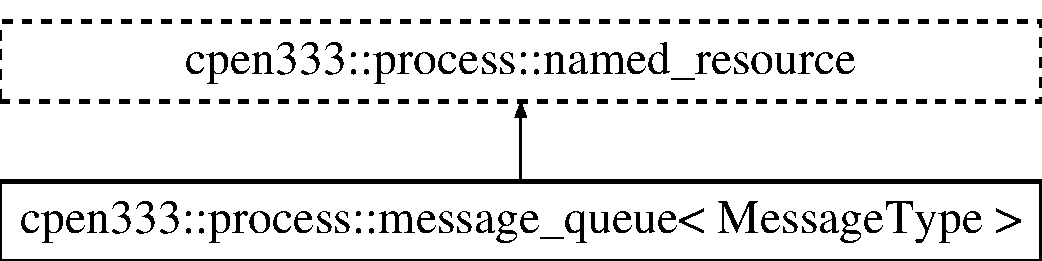
\includegraphics[height=2.000000cm]{classcpen333_1_1process_1_1message__queue}
\end{center}
\end{figure}
\subsection*{Public Types}
\begin{DoxyCompactItemize}
\item 
\mbox{\Hypertarget{classcpen333_1_1process_1_1message__queue_a846d3e301643761369a88933f3fb282b}\label{classcpen333_1_1process_1_1message__queue_a846d3e301643761369a88933f3fb282b}} 
typedef Message\+Type \hyperlink{classcpen333_1_1process_1_1message__queue_a846d3e301643761369a88933f3fb282b}{message\+\_\+type}
\begin{DoxyCompactList}\small\item\em Message type. \end{DoxyCompactList}\end{DoxyCompactItemize}
\subsection*{Public Member Functions}
\begin{DoxyCompactItemize}
\item 
\hyperlink{classcpen333_1_1process_1_1message__queue_a3312decb9ec69e323ba97f321125d348}{message\+\_\+queue} (const std\+::string \&name, size\+\_\+t \hyperlink{classcpen333_1_1process_1_1message__queue_aab604a8c153f7f918762abc7f2380396}{size}=1024)
\begin{DoxyCompactList}\small\item\em Constructs a named message queue. \end{DoxyCompactList}\item 
void \hyperlink{classcpen333_1_1process_1_1message__queue_a1f50c208f75ad2937d11d7eca8fdb6f0}{send} (const Message\+Type \&msg)
\begin{DoxyCompactList}\small\item\em Sends a message to the queue. \end{DoxyCompactList}\item 
bool \hyperlink{classcpen333_1_1process_1_1message__queue_ae632a2b200bdac5bc93039b9bcb3d7f5}{try\+\_\+send} (const Message\+Type \&msg)
\begin{DoxyCompactList}\small\item\em Tries to send a message without blocking. \end{DoxyCompactList}\item 
{\footnotesize template$<$typename Rep , typename Period $>$ }\\bool \hyperlink{classcpen333_1_1process_1_1message__queue_a5242a6193a42e68e36634846f09c5e3b}{try\+\_\+send\+\_\+for} (const Message\+Type \&msg, std\+::chrono\+::duration$<$ Rep, Period $>$ \&rel\+\_\+time)
\begin{DoxyCompactList}\small\item\em Tries to send a message, will wait for a maximum amount of time before aborting. \end{DoxyCompactList}\item 
{\footnotesize template$<$typename Clock , typename Duration $>$ }\\bool \hyperlink{classcpen333_1_1process_1_1message__queue_ab13d8f1c89ca9022e5446b3fc5432072}{try\+\_\+send\+\_\+until} (const Message\+Type \&msg, const std\+::chrono\+::time\+\_\+point$<$ Clock, Duration $>$ \&timeout)
\begin{DoxyCompactList}\small\item\em Tries to send a message, will wait until a timeout time has been reached before aborting. \end{DoxyCompactList}\item 
Message\+Type \hyperlink{classcpen333_1_1process_1_1message__queue_a39d2e54480fba6a441e70cb1362d3900}{receive} ()
\begin{DoxyCompactList}\small\item\em Retrieves and removes the next message from the message queue. \end{DoxyCompactList}\item 
void \hyperlink{classcpen333_1_1process_1_1message__queue_a63eccb93a61129e6e6dec2db5f5b1f2b}{receive} (Message\+Type $\ast$out)
\begin{DoxyCompactList}\small\item\em Retrieves and removes the next message from the message queue. \end{DoxyCompactList}\item 
bool \hyperlink{classcpen333_1_1process_1_1message__queue_ae42a9bd9edc9753a38fa63f20a34cc60}{try\+\_\+receive} (Message\+Type $\ast$out)
\begin{DoxyCompactList}\small\item\em Tries to receive a message without blocking. \end{DoxyCompactList}\item 
{\footnotesize template$<$typename Rep , typename Period $>$ }\\bool \hyperlink{classcpen333_1_1process_1_1message__queue_a4264047863208a01109569f62d093885}{try\+\_\+receive\+\_\+for} (Message\+Type $\ast$out, std\+::chrono\+::duration$<$ Rep, Period $>$ \&rel\+\_\+time)
\begin{DoxyCompactList}\small\item\em Tries to receive a message, will wait for a maximum amount of time before aborting. \end{DoxyCompactList}\item 
{\footnotesize template$<$typename Clock , typename Duration $>$ }\\bool \hyperlink{classcpen333_1_1process_1_1message__queue_abf193426822dfbb27fc1ce972db42da0}{try\+\_\+receive\+\_\+until} (Message\+Type $\ast$out, const std\+::chrono\+::time\+\_\+point$<$ Clock, Duration $>$ \&timeout)
\begin{DoxyCompactList}\small\item\em Tries to receive a message, will wait for a maximum timeout time to be reached before aborting. \end{DoxyCompactList}\item 
Message\+Type \hyperlink{classcpen333_1_1process_1_1message__queue_a22e2c27bc1fe660b573129f7518ecec7}{peek} ()
\begin{DoxyCompactList}\small\item\em Peeks at the next message without removing it. \end{DoxyCompactList}\item 
void \hyperlink{classcpen333_1_1process_1_1message__queue_a0d6f0bb9911b01f601bb67551007be3d}{peek} (Message\+Type $\ast$out)
\begin{DoxyCompactList}\small\item\em Peeks at the next message without removing it. \end{DoxyCompactList}\item 
bool \hyperlink{classcpen333_1_1process_1_1message__queue_a344d81de71e73ab318d2bf4a4a852a1b}{try\+\_\+peek} (Message\+Type $\ast$out)
\begin{DoxyCompactList}\small\item\em Tries to peek at the message without blocking. \end{DoxyCompactList}\item 
{\footnotesize template$<$typename Rep , typename Period $>$ }\\bool \hyperlink{classcpen333_1_1process_1_1message__queue_a62077115caee87a6eccd527924015748}{try\+\_\+peek\+\_\+for} (Message\+Type $\ast$out, std\+::chrono\+::duration$<$ Rep, Period $>$ \&rel\+\_\+time)
\begin{DoxyCompactList}\small\item\em Tries to peek at the next message, will wait for a maximum amount of time before aborting. \end{DoxyCompactList}\item 
{\footnotesize template$<$typename Clock , typename Duration $>$ }\\bool \hyperlink{classcpen333_1_1process_1_1message__queue_ae518346095033df725270dfeb866cdb4}{try\+\_\+peek\+\_\+until} (Message\+Type $\ast$out, const std\+::chrono\+::time\+\_\+point$<$ Clock, Duration $>$ \&timeout)
\begin{DoxyCompactList}\small\item\em Tries to peek at the next message, will wait for a maximum timeout time before aborting. \end{DoxyCompactList}\item 
size\+\_\+t \hyperlink{classcpen333_1_1process_1_1message__queue_aab604a8c153f7f918762abc7f2380396}{size} ()
\begin{DoxyCompactList}\small\item\em Number of messages currently in the queue. \end{DoxyCompactList}\item 
bool \hyperlink{classcpen333_1_1process_1_1message__queue_a321bee9b732f97362172c6c4ee8226a4}{empty} ()
\begin{DoxyCompactList}\small\item\em Check if the message queue is currently empty. \end{DoxyCompactList}\item 
bool \hyperlink{classcpen333_1_1process_1_1message__queue_ae94a6503dff948dfc2533f7786839dca}{unlink} ()
\begin{DoxyCompactList}\small\item\em Detaches the name from the named resource. \end{DoxyCompactList}\end{DoxyCompactItemize}
\subsection*{Static Public Member Functions}
\begin{DoxyCompactItemize}
\item 
static bool \hyperlink{classcpen333_1_1process_1_1message__queue_aca172436d5b30c250c301d3c224598b6}{unlink} (const std\+::string \&name)
\begin{DoxyCompactList}\small\item\em Unlinks the name without needing to create a resource. \end{DoxyCompactList}\end{DoxyCompactItemize}


\subsection{Detailed Description}
\subsubsection*{template$<$typename Message\+Type$>$\newline
class cpen333\+::process\+::message\+\_\+queue$<$ Message\+Type $>$}

Basic inter-\/process named message queue based on a F\+I\+FO. 

Allows sending/receiving of messages with a fixed type. Unlike Windows messages, does not require you to know the thread ID of the receiver, but also does not allow filtering on the receiving end. Unlike a P\+O\+S\+IX message queue, does not allow variable length messages or message priorities.


\begin{DoxyTemplParams}{Template Parameters}
{\em Message\+Type} & fixed type of messages. \\
\hline
\end{DoxyTemplParams}


\subsection{Constructor \& Destructor Documentation}
\mbox{\Hypertarget{classcpen333_1_1process_1_1message__queue_a3312decb9ec69e323ba97f321125d348}\label{classcpen333_1_1process_1_1message__queue_a3312decb9ec69e323ba97f321125d348}} 
\index{cpen333\+::process\+::message\+\_\+queue@{cpen333\+::process\+::message\+\_\+queue}!message\+\_\+queue@{message\+\_\+queue}}
\index{message\+\_\+queue@{message\+\_\+queue}!cpen333\+::process\+::message\+\_\+queue@{cpen333\+::process\+::message\+\_\+queue}}
\subsubsection{\texorpdfstring{message\+\_\+queue()}{message\_queue()}}
{\footnotesize\ttfamily template$<$typename Message\+Type $>$ \\
\hyperlink{classcpen333_1_1process_1_1message__queue}{cpen333\+::process\+::message\+\_\+queue}$<$ Message\+Type $>$\+::\hyperlink{classcpen333_1_1process_1_1message__queue}{message\+\_\+queue} (\begin{DoxyParamCaption}\item[{const std\+::string \&}]{name,  }\item[{size\+\_\+t}]{size = {\ttfamily 1024} }\end{DoxyParamCaption})\hspace{0.3cm}{\ttfamily [inline]}}



Constructs a named message queue. 


\begin{DoxyParams}{Parameters}
{\em name} & name identifier for creating or connecting to an existing inter-\/process message-\/queue \\
\hline
{\em size} & if creating, the maximum number of elements that can be stored in the queue without blocking \\
\hline
\end{DoxyParams}


\subsection{Member Function Documentation}
\mbox{\Hypertarget{classcpen333_1_1process_1_1message__queue_a321bee9b732f97362172c6c4ee8226a4}\label{classcpen333_1_1process_1_1message__queue_a321bee9b732f97362172c6c4ee8226a4}} 
\index{cpen333\+::process\+::message\+\_\+queue@{cpen333\+::process\+::message\+\_\+queue}!empty@{empty}}
\index{empty@{empty}!cpen333\+::process\+::message\+\_\+queue@{cpen333\+::process\+::message\+\_\+queue}}
\subsubsection{\texorpdfstring{empty()}{empty()}}
{\footnotesize\ttfamily template$<$typename Message\+Type $>$ \\
bool \hyperlink{classcpen333_1_1process_1_1message__queue}{cpen333\+::process\+::message\+\_\+queue}$<$ Message\+Type $>$\+::empty (\begin{DoxyParamCaption}{ }\end{DoxyParamCaption})\hspace{0.3cm}{\ttfamily [inline]}}



Check if the message queue is currently empty. 

This method should be used sparingly, since messages could be added/removed during or immediately after the call, making the result potentially unreliable

\begin{DoxyReturn}{Returns}
{\ttfamily true} if empty, {\ttfamily false} otherwise 
\end{DoxyReturn}
\mbox{\Hypertarget{classcpen333_1_1process_1_1message__queue_a22e2c27bc1fe660b573129f7518ecec7}\label{classcpen333_1_1process_1_1message__queue_a22e2c27bc1fe660b573129f7518ecec7}} 
\index{cpen333\+::process\+::message\+\_\+queue@{cpen333\+::process\+::message\+\_\+queue}!peek@{peek}}
\index{peek@{peek}!cpen333\+::process\+::message\+\_\+queue@{cpen333\+::process\+::message\+\_\+queue}}
\subsubsection{\texorpdfstring{peek()}{peek()}\hspace{0.1cm}{\footnotesize\ttfamily [1/2]}}
{\footnotesize\ttfamily template$<$typename Message\+Type $>$ \\
Message\+Type \hyperlink{classcpen333_1_1process_1_1message__queue}{cpen333\+::process\+::message\+\_\+queue}$<$ Message\+Type $>$\+::peek (\begin{DoxyParamCaption}{ }\end{DoxyParamCaption})\hspace{0.3cm}{\ttfamily [inline]}}



Peeks at the next message without removing it. 

Returns the next message in the queue. If there are currently no messages, this method will block until one becomes available. The message will remain in the queue for the next {\ttfamily peek} or {\ttfamily receive} operation.

\begin{DoxyReturn}{Returns}
next message in the queue 
\end{DoxyReturn}
\mbox{\Hypertarget{classcpen333_1_1process_1_1message__queue_a0d6f0bb9911b01f601bb67551007be3d}\label{classcpen333_1_1process_1_1message__queue_a0d6f0bb9911b01f601bb67551007be3d}} 
\index{cpen333\+::process\+::message\+\_\+queue@{cpen333\+::process\+::message\+\_\+queue}!peek@{peek}}
\index{peek@{peek}!cpen333\+::process\+::message\+\_\+queue@{cpen333\+::process\+::message\+\_\+queue}}
\subsubsection{\texorpdfstring{peek()}{peek()}\hspace{0.1cm}{\footnotesize\ttfamily [2/2]}}
{\footnotesize\ttfamily template$<$typename Message\+Type $>$ \\
void \hyperlink{classcpen333_1_1process_1_1message__queue}{cpen333\+::process\+::message\+\_\+queue}$<$ Message\+Type $>$\+::peek (\begin{DoxyParamCaption}\item[{Message\+Type $\ast$}]{out }\end{DoxyParamCaption})\hspace{0.3cm}{\ttfamily [inline]}}



Peeks at the next message without removing it. 

Populates memory pointed to by {\ttfamily out} with next message in the queue. If there are currently no messages, this method will block until a message becomes available. The message will remain in the queue for the next {\ttfamily peek} or {\ttfamily receive} operation.


\begin{DoxyParams}{Parameters}
{\em out} & destination. If {\ttfamily nullptr}, nothing happens. \\
\hline
\end{DoxyParams}
\mbox{\Hypertarget{classcpen333_1_1process_1_1message__queue_a39d2e54480fba6a441e70cb1362d3900}\label{classcpen333_1_1process_1_1message__queue_a39d2e54480fba6a441e70cb1362d3900}} 
\index{cpen333\+::process\+::message\+\_\+queue@{cpen333\+::process\+::message\+\_\+queue}!receive@{receive}}
\index{receive@{receive}!cpen333\+::process\+::message\+\_\+queue@{cpen333\+::process\+::message\+\_\+queue}}
\subsubsection{\texorpdfstring{receive()}{receive()}\hspace{0.1cm}{\footnotesize\ttfamily [1/2]}}
{\footnotesize\ttfamily template$<$typename Message\+Type $>$ \\
Message\+Type \hyperlink{classcpen333_1_1process_1_1message__queue}{cpen333\+::process\+::message\+\_\+queue}$<$ Message\+Type $>$\+::receive (\begin{DoxyParamCaption}{ }\end{DoxyParamCaption})\hspace{0.3cm}{\ttfamily [inline]}}



Retrieves and removes the next message from the message queue. 

If there are currently no messages in the queue, then the current thread will block until a message becomes available.

\begin{DoxyReturn}{Returns}
the next message in the queue 
\end{DoxyReturn}
\mbox{\Hypertarget{classcpen333_1_1process_1_1message__queue_a63eccb93a61129e6e6dec2db5f5b1f2b}\label{classcpen333_1_1process_1_1message__queue_a63eccb93a61129e6e6dec2db5f5b1f2b}} 
\index{cpen333\+::process\+::message\+\_\+queue@{cpen333\+::process\+::message\+\_\+queue}!receive@{receive}}
\index{receive@{receive}!cpen333\+::process\+::message\+\_\+queue@{cpen333\+::process\+::message\+\_\+queue}}
\subsubsection{\texorpdfstring{receive()}{receive()}\hspace{0.1cm}{\footnotesize\ttfamily [2/2]}}
{\footnotesize\ttfamily template$<$typename Message\+Type $>$ \\
void \hyperlink{classcpen333_1_1process_1_1message__queue}{cpen333\+::process\+::message\+\_\+queue}$<$ Message\+Type $>$\+::receive (\begin{DoxyParamCaption}\item[{Message\+Type $\ast$}]{out }\end{DoxyParamCaption})\hspace{0.3cm}{\ttfamily [inline]}}



Retrieves and removes the next message from the message queue. 

If there are currently no messages in the queue, then the current thread will block until a message becomes available.


\begin{DoxyParams}{Parameters}
{\em out} & destination. If {\ttfamily nullptr}, the message is removed from the queue but not returned \\
\hline
\end{DoxyParams}
\mbox{\Hypertarget{classcpen333_1_1process_1_1message__queue_a1f50c208f75ad2937d11d7eca8fdb6f0}\label{classcpen333_1_1process_1_1message__queue_a1f50c208f75ad2937d11d7eca8fdb6f0}} 
\index{cpen333\+::process\+::message\+\_\+queue@{cpen333\+::process\+::message\+\_\+queue}!send@{send}}
\index{send@{send}!cpen333\+::process\+::message\+\_\+queue@{cpen333\+::process\+::message\+\_\+queue}}
\subsubsection{\texorpdfstring{send()}{send()}}
{\footnotesize\ttfamily template$<$typename Message\+Type $>$ \\
void \hyperlink{classcpen333_1_1process_1_1message__queue}{cpen333\+::process\+::message\+\_\+queue}$<$ Message\+Type $>$\+::send (\begin{DoxyParamCaption}\item[{const Message\+Type \&}]{msg }\end{DoxyParamCaption})\hspace{0.3cm}{\ttfamily [inline]}}



Sends a message to the queue. 


\begin{DoxyParams}{Parameters}
{\em msg} & message to send \\
\hline
\end{DoxyParams}
\mbox{\Hypertarget{classcpen333_1_1process_1_1message__queue_aab604a8c153f7f918762abc7f2380396}\label{classcpen333_1_1process_1_1message__queue_aab604a8c153f7f918762abc7f2380396}} 
\index{cpen333\+::process\+::message\+\_\+queue@{cpen333\+::process\+::message\+\_\+queue}!size@{size}}
\index{size@{size}!cpen333\+::process\+::message\+\_\+queue@{cpen333\+::process\+::message\+\_\+queue}}
\subsubsection{\texorpdfstring{size()}{size()}}
{\footnotesize\ttfamily template$<$typename Message\+Type $>$ \\
size\+\_\+t \hyperlink{classcpen333_1_1process_1_1message__queue}{cpen333\+::process\+::message\+\_\+queue}$<$ Message\+Type $>$\+::size (\begin{DoxyParamCaption}{ }\end{DoxyParamCaption})\hspace{0.3cm}{\ttfamily [inline]}}



Number of messages currently in the queue. 

This method should be used sparingly, since messages could be added/removed during or immediately after the call, making the result potentially unreliable.

\begin{DoxyReturn}{Returns}
number of messages 
\end{DoxyReturn}
\mbox{\Hypertarget{classcpen333_1_1process_1_1message__queue_a344d81de71e73ab318d2bf4a4a852a1b}\label{classcpen333_1_1process_1_1message__queue_a344d81de71e73ab318d2bf4a4a852a1b}} 
\index{cpen333\+::process\+::message\+\_\+queue@{cpen333\+::process\+::message\+\_\+queue}!try\+\_\+peek@{try\+\_\+peek}}
\index{try\+\_\+peek@{try\+\_\+peek}!cpen333\+::process\+::message\+\_\+queue@{cpen333\+::process\+::message\+\_\+queue}}
\subsubsection{\texorpdfstring{try\+\_\+peek()}{try\_peek()}}
{\footnotesize\ttfamily template$<$typename Message\+Type $>$ \\
bool \hyperlink{classcpen333_1_1process_1_1message__queue}{cpen333\+::process\+::message\+\_\+queue}$<$ Message\+Type $>$\+::try\+\_\+peek (\begin{DoxyParamCaption}\item[{Message\+Type $\ast$}]{out }\end{DoxyParamCaption})\hspace{0.3cm}{\ttfamily [inline]}}



Tries to peek at the message without blocking. 

Populates memory pointed to by {\ttfamily out} with the next message in the queue. If there are no messages, then this will return immediately without peeking. The message will remain in the queue for the next {\ttfamily peek} or {\ttfamily receive} operation.


\begin{DoxyParams}{Parameters}
{\em out} & destination. If {\ttfamily nullptr}, nothing happens. \\
\hline
\end{DoxyParams}
\begin{DoxyReturn}{Returns}
{\ttfamily true} if message was successfully peeked, {\ttfamily false} otherwise 
\end{DoxyReturn}
\mbox{\Hypertarget{classcpen333_1_1process_1_1message__queue_a62077115caee87a6eccd527924015748}\label{classcpen333_1_1process_1_1message__queue_a62077115caee87a6eccd527924015748}} 
\index{cpen333\+::process\+::message\+\_\+queue@{cpen333\+::process\+::message\+\_\+queue}!try\+\_\+peek\+\_\+for@{try\+\_\+peek\+\_\+for}}
\index{try\+\_\+peek\+\_\+for@{try\+\_\+peek\+\_\+for}!cpen333\+::process\+::message\+\_\+queue@{cpen333\+::process\+::message\+\_\+queue}}
\subsubsection{\texorpdfstring{try\+\_\+peek\+\_\+for()}{try\_peek\_for()}}
{\footnotesize\ttfamily template$<$typename Message\+Type $>$ \\
template$<$typename Rep , typename Period $>$ \\
bool \hyperlink{classcpen333_1_1process_1_1message__queue}{cpen333\+::process\+::message\+\_\+queue}$<$ Message\+Type $>$\+::try\+\_\+peek\+\_\+for (\begin{DoxyParamCaption}\item[{Message\+Type $\ast$}]{out,  }\item[{std\+::chrono\+::duration$<$ Rep, Period $>$ \&}]{rel\+\_\+time }\end{DoxyParamCaption})\hspace{0.3cm}{\ttfamily [inline]}}



Tries to peek at the next message, will wait for a maximum amount of time before aborting. 

If it is not possible to peek at the next message immediately, then the current thread will block until either a message becomes available, or a timeout period has elapsed. The message will remain in the queue for the next {\ttfamily peek} or {\ttfamily receive} operation.


\begin{DoxyTemplParams}{Template Parameters}
{\em Rep} & duration representation \\
\hline
{\em Period} & duration period \\
\hline
\end{DoxyTemplParams}

\begin{DoxyParams}{Parameters}
{\em out} & destination. If {\ttfamily nullptr}, nothing happens \\
\hline
{\em rel\+\_\+time} & relative timeout time \\
\hline
\end{DoxyParams}
\begin{DoxyReturn}{Returns}
{\ttfamily true} if message successfully peeked, {\ttfamily false} if timeout elapsed 
\end{DoxyReturn}
\mbox{\Hypertarget{classcpen333_1_1process_1_1message__queue_ae518346095033df725270dfeb866cdb4}\label{classcpen333_1_1process_1_1message__queue_ae518346095033df725270dfeb866cdb4}} 
\index{cpen333\+::process\+::message\+\_\+queue@{cpen333\+::process\+::message\+\_\+queue}!try\+\_\+peek\+\_\+until@{try\+\_\+peek\+\_\+until}}
\index{try\+\_\+peek\+\_\+until@{try\+\_\+peek\+\_\+until}!cpen333\+::process\+::message\+\_\+queue@{cpen333\+::process\+::message\+\_\+queue}}
\subsubsection{\texorpdfstring{try\+\_\+peek\+\_\+until()}{try\_peek\_until()}}
{\footnotesize\ttfamily template$<$typename Message\+Type $>$ \\
template$<$typename Clock , typename Duration $>$ \\
bool \hyperlink{classcpen333_1_1process_1_1message__queue}{cpen333\+::process\+::message\+\_\+queue}$<$ Message\+Type $>$\+::try\+\_\+peek\+\_\+until (\begin{DoxyParamCaption}\item[{Message\+Type $\ast$}]{out,  }\item[{const std\+::chrono\+::time\+\_\+point$<$ Clock, Duration $>$ \&}]{timeout }\end{DoxyParamCaption})\hspace{0.3cm}{\ttfamily [inline]}}



Tries to peek at the next message, will wait for a maximum timeout time before aborting. 

If it is not possible to peek at the next message immediately, then the current thread will block until either a message becomes available, or a timeout time has been reached. The message will remain in the queue for the next {\ttfamily peek} or {\ttfamily receive} operation.


\begin{DoxyTemplParams}{Template Parameters}
{\em Clock} & clock type \\
\hline
{\em Duration} & clock duration type \\
\hline
\end{DoxyTemplParams}

\begin{DoxyParams}{Parameters}
{\em out} & destination. If {\ttfamily nullptr}, nothing happens \\
\hline
{\em timeout} & absolute timeout time \\
\hline
\end{DoxyParams}
\begin{DoxyReturn}{Returns}
{\ttfamily true} if message successfully peeked, {\ttfamily false} if timeout 
\end{DoxyReturn}
\mbox{\Hypertarget{classcpen333_1_1process_1_1message__queue_ae42a9bd9edc9753a38fa63f20a34cc60}\label{classcpen333_1_1process_1_1message__queue_ae42a9bd9edc9753a38fa63f20a34cc60}} 
\index{cpen333\+::process\+::message\+\_\+queue@{cpen333\+::process\+::message\+\_\+queue}!try\+\_\+receive@{try\+\_\+receive}}
\index{try\+\_\+receive@{try\+\_\+receive}!cpen333\+::process\+::message\+\_\+queue@{cpen333\+::process\+::message\+\_\+queue}}
\subsubsection{\texorpdfstring{try\+\_\+receive()}{try\_receive()}}
{\footnotesize\ttfamily template$<$typename Message\+Type $>$ \\
bool \hyperlink{classcpen333_1_1process_1_1message__queue}{cpen333\+::process\+::message\+\_\+queue}$<$ Message\+Type $>$\+::try\+\_\+receive (\begin{DoxyParamCaption}\item[{Message\+Type $\ast$}]{out }\end{DoxyParamCaption})\hspace{0.3cm}{\ttfamily [inline]}}



Tries to receive a message without blocking. 

Populates memory pointed to by {\ttfamily out} with the next message, and removes the message from the queue. If there are no messages, then this will return immediately.


\begin{DoxyParams}{Parameters}
{\em out} & destination. If {\ttfamily nullptr}, the message is removed but not returned. \\
\hline
\end{DoxyParams}
\begin{DoxyReturn}{Returns}
{\ttfamily true} if a message is returned, {\ttfamily false} otherwise 
\end{DoxyReturn}
\mbox{\Hypertarget{classcpen333_1_1process_1_1message__queue_a4264047863208a01109569f62d093885}\label{classcpen333_1_1process_1_1message__queue_a4264047863208a01109569f62d093885}} 
\index{cpen333\+::process\+::message\+\_\+queue@{cpen333\+::process\+::message\+\_\+queue}!try\+\_\+receive\+\_\+for@{try\+\_\+receive\+\_\+for}}
\index{try\+\_\+receive\+\_\+for@{try\+\_\+receive\+\_\+for}!cpen333\+::process\+::message\+\_\+queue@{cpen333\+::process\+::message\+\_\+queue}}
\subsubsection{\texorpdfstring{try\+\_\+receive\+\_\+for()}{try\_receive\_for()}}
{\footnotesize\ttfamily template$<$typename Message\+Type $>$ \\
template$<$typename Rep , typename Period $>$ \\
bool \hyperlink{classcpen333_1_1process_1_1message__queue}{cpen333\+::process\+::message\+\_\+queue}$<$ Message\+Type $>$\+::try\+\_\+receive\+\_\+for (\begin{DoxyParamCaption}\item[{Message\+Type $\ast$}]{out,  }\item[{std\+::chrono\+::duration$<$ Rep, Period $>$ \&}]{rel\+\_\+time }\end{DoxyParamCaption})\hspace{0.3cm}{\ttfamily [inline]}}



Tries to receive a message, will wait for a maximum amount of time before aborting. 

If it is not possible to receive a message immediately, then the current thread will block until either a message becomes available, or a timeout period has elapsed.


\begin{DoxyTemplParams}{Template Parameters}
{\em Rep} & duration representation \\
\hline
{\em Period} & duration period \\
\hline
\end{DoxyTemplParams}

\begin{DoxyParams}{Parameters}
{\em out} & destination. If {\ttfamily nullptr}, the next message is removed but not returned \\
\hline
{\em rel\+\_\+time} & relative timeout time \\
\hline
\end{DoxyParams}
\begin{DoxyReturn}{Returns}
{\ttfamily true} if message successfully returned, {\ttfamily false} if timeout elapsed 
\end{DoxyReturn}
\mbox{\Hypertarget{classcpen333_1_1process_1_1message__queue_abf193426822dfbb27fc1ce972db42da0}\label{classcpen333_1_1process_1_1message__queue_abf193426822dfbb27fc1ce972db42da0}} 
\index{cpen333\+::process\+::message\+\_\+queue@{cpen333\+::process\+::message\+\_\+queue}!try\+\_\+receive\+\_\+until@{try\+\_\+receive\+\_\+until}}
\index{try\+\_\+receive\+\_\+until@{try\+\_\+receive\+\_\+until}!cpen333\+::process\+::message\+\_\+queue@{cpen333\+::process\+::message\+\_\+queue}}
\subsubsection{\texorpdfstring{try\+\_\+receive\+\_\+until()}{try\_receive\_until()}}
{\footnotesize\ttfamily template$<$typename Message\+Type $>$ \\
template$<$typename Clock , typename Duration $>$ \\
bool \hyperlink{classcpen333_1_1process_1_1message__queue}{cpen333\+::process\+::message\+\_\+queue}$<$ Message\+Type $>$\+::try\+\_\+receive\+\_\+until (\begin{DoxyParamCaption}\item[{Message\+Type $\ast$}]{out,  }\item[{const std\+::chrono\+::time\+\_\+point$<$ Clock, Duration $>$ \&}]{timeout }\end{DoxyParamCaption})\hspace{0.3cm}{\ttfamily [inline]}}



Tries to receive a message, will wait for a maximum timeout time to be reached before aborting. 

If it is not possible to receive a message immediately, then the current thread will block until either a message becomes available, or a timeout time has been reached.


\begin{DoxyTemplParams}{Template Parameters}
{\em Clock} & clock type \\
\hline
{\em Duration} & clock duration type \\
\hline
\end{DoxyTemplParams}

\begin{DoxyParams}{Parameters}
{\em out} & destination. If {\ttfamily nullptr}, the next message is removed but not returned \\
\hline
{\em timeout} & absolute timeout time \\
\hline
\end{DoxyParams}
\begin{DoxyReturn}{Returns}
{\ttfamily true} if message successfully returned, {\ttfamily false} if timeout 
\end{DoxyReturn}
\mbox{\Hypertarget{classcpen333_1_1process_1_1message__queue_ae632a2b200bdac5bc93039b9bcb3d7f5}\label{classcpen333_1_1process_1_1message__queue_ae632a2b200bdac5bc93039b9bcb3d7f5}} 
\index{cpen333\+::process\+::message\+\_\+queue@{cpen333\+::process\+::message\+\_\+queue}!try\+\_\+send@{try\+\_\+send}}
\index{try\+\_\+send@{try\+\_\+send}!cpen333\+::process\+::message\+\_\+queue@{cpen333\+::process\+::message\+\_\+queue}}
\subsubsection{\texorpdfstring{try\+\_\+send()}{try\_send()}}
{\footnotesize\ttfamily template$<$typename Message\+Type $>$ \\
bool \hyperlink{classcpen333_1_1process_1_1message__queue}{cpen333\+::process\+::message\+\_\+queue}$<$ Message\+Type $>$\+::try\+\_\+send (\begin{DoxyParamCaption}\item[{const Message\+Type \&}]{msg }\end{DoxyParamCaption})\hspace{0.3cm}{\ttfamily [inline]}}



Tries to send a message without blocking. 

If it is not possible to send the message without blocking, then will return immediately without sending.


\begin{DoxyParams}{Parameters}
{\em msg} & message to send \\
\hline
\end{DoxyParams}
\begin{DoxyReturn}{Returns}
{\ttfamily true} if message sent successfully, {\ttfamily false} if not sent 
\end{DoxyReturn}
\mbox{\Hypertarget{classcpen333_1_1process_1_1message__queue_a5242a6193a42e68e36634846f09c5e3b}\label{classcpen333_1_1process_1_1message__queue_a5242a6193a42e68e36634846f09c5e3b}} 
\index{cpen333\+::process\+::message\+\_\+queue@{cpen333\+::process\+::message\+\_\+queue}!try\+\_\+send\+\_\+for@{try\+\_\+send\+\_\+for}}
\index{try\+\_\+send\+\_\+for@{try\+\_\+send\+\_\+for}!cpen333\+::process\+::message\+\_\+queue@{cpen333\+::process\+::message\+\_\+queue}}
\subsubsection{\texorpdfstring{try\+\_\+send\+\_\+for()}{try\_send\_for()}}
{\footnotesize\ttfamily template$<$typename Message\+Type $>$ \\
template$<$typename Rep , typename Period $>$ \\
bool \hyperlink{classcpen333_1_1process_1_1message__queue}{cpen333\+::process\+::message\+\_\+queue}$<$ Message\+Type $>$\+::try\+\_\+send\+\_\+for (\begin{DoxyParamCaption}\item[{const Message\+Type \&}]{msg,  }\item[{std\+::chrono\+::duration$<$ Rep, Period $>$ \&}]{rel\+\_\+time }\end{DoxyParamCaption})\hspace{0.3cm}{\ttfamily [inline]}}



Tries to send a message, will wait for a maximum amount of time before aborting. 

If it is not possible to send the message immediately, then the current thread will block until either the message is sent successfully, or a timeout period has elapsed.


\begin{DoxyTemplParams}{Template Parameters}
{\em Rep} & timeout duration representation \\
\hline
{\em Period} & timeout duration period \\
\hline
\end{DoxyTemplParams}

\begin{DoxyParams}{Parameters}
{\em msg} & message to send \\
\hline
{\em rel\+\_\+time} & relative timeout time \\
\hline
\end{DoxyParams}
\begin{DoxyReturn}{Returns}
{\ttfamily true} if the message is sent successfully within the timeout period, {\ttfamily false} if not sent 
\end{DoxyReturn}
\mbox{\Hypertarget{classcpen333_1_1process_1_1message__queue_ab13d8f1c89ca9022e5446b3fc5432072}\label{classcpen333_1_1process_1_1message__queue_ab13d8f1c89ca9022e5446b3fc5432072}} 
\index{cpen333\+::process\+::message\+\_\+queue@{cpen333\+::process\+::message\+\_\+queue}!try\+\_\+send\+\_\+until@{try\+\_\+send\+\_\+until}}
\index{try\+\_\+send\+\_\+until@{try\+\_\+send\+\_\+until}!cpen333\+::process\+::message\+\_\+queue@{cpen333\+::process\+::message\+\_\+queue}}
\subsubsection{\texorpdfstring{try\+\_\+send\+\_\+until()}{try\_send\_until()}}
{\footnotesize\ttfamily template$<$typename Message\+Type $>$ \\
template$<$typename Clock , typename Duration $>$ \\
bool \hyperlink{classcpen333_1_1process_1_1message__queue}{cpen333\+::process\+::message\+\_\+queue}$<$ Message\+Type $>$\+::try\+\_\+send\+\_\+until (\begin{DoxyParamCaption}\item[{const Message\+Type \&}]{msg,  }\item[{const std\+::chrono\+::time\+\_\+point$<$ Clock, Duration $>$ \&}]{timeout }\end{DoxyParamCaption})\hspace{0.3cm}{\ttfamily [inline]}}



Tries to send a message, will wait until a timeout time has been reached before aborting. 

If it is not possible to send the message immediately, then the current thread will block until either the message is sent successfully, or an absolute timeout time has been reached.


\begin{DoxyTemplParams}{Template Parameters}
{\em Clock} & timeout clock type \\
\hline
{\em Duration} & timeout duration type \\
\hline
\end{DoxyTemplParams}

\begin{DoxyParams}{Parameters}
{\em msg} & message to send \\
\hline
{\em timeout} & absolute timeout time \\
\hline
\end{DoxyParams}
\begin{DoxyReturn}{Returns}
{\ttfamily true} if message sent successfully before timeout time has passed, {\ttfamily false} if message not sent 
\end{DoxyReturn}
\mbox{\Hypertarget{classcpen333_1_1process_1_1message__queue_ae94a6503dff948dfc2533f7786839dca}\label{classcpen333_1_1process_1_1message__queue_ae94a6503dff948dfc2533f7786839dca}} 
\index{cpen333\+::process\+::message\+\_\+queue@{cpen333\+::process\+::message\+\_\+queue}!unlink@{unlink}}
\index{unlink@{unlink}!cpen333\+::process\+::message\+\_\+queue@{cpen333\+::process\+::message\+\_\+queue}}
\subsubsection{\texorpdfstring{unlink()}{unlink()}\hspace{0.1cm}{\footnotesize\ttfamily [1/2]}}
{\footnotesize\ttfamily template$<$typename Message\+Type $>$ \\
bool \hyperlink{classcpen333_1_1process_1_1message__queue}{cpen333\+::process\+::message\+\_\+queue}$<$ Message\+Type $>$\+::unlink (\begin{DoxyParamCaption}{ }\end{DoxyParamCaption})\hspace{0.3cm}{\ttfamily [inline]}, {\ttfamily [virtual]}}



Detaches the name from the named resource. 

On P\+O\+S\+IX systems, named resources will persist beyond the lifetime of any process that uses them as long as the name has not been unlinked (or until the system is rebooted). Calling {\ttfamily unlink} will detach the name, allowing the resource to be freed once all current users have exited.

\begin{DoxyReturn}{Returns}
{\ttfamily true} if unlink is successful, {\ttfamily false} if unlinking is not supported or if an error has occurred. 
\end{DoxyReturn}


Implements \hyperlink{classcpen333_1_1process_1_1named__resource_a5d33168fee48c9b0c58ab8fd96e230ce}{cpen333\+::process\+::named\+\_\+resource}.

\mbox{\Hypertarget{classcpen333_1_1process_1_1message__queue_aca172436d5b30c250c301d3c224598b6}\label{classcpen333_1_1process_1_1message__queue_aca172436d5b30c250c301d3c224598b6}} 
\index{cpen333\+::process\+::message\+\_\+queue@{cpen333\+::process\+::message\+\_\+queue}!unlink@{unlink}}
\index{unlink@{unlink}!cpen333\+::process\+::message\+\_\+queue@{cpen333\+::process\+::message\+\_\+queue}}
\subsubsection{\texorpdfstring{unlink()}{unlink()}\hspace{0.1cm}{\footnotesize\ttfamily [2/2]}}
{\footnotesize\ttfamily template$<$typename Message\+Type $>$ \\
static bool \hyperlink{classcpen333_1_1process_1_1message__queue}{cpen333\+::process\+::message\+\_\+queue}$<$ Message\+Type $>$\+::unlink (\begin{DoxyParamCaption}\item[{const std\+::string \&}]{name }\end{DoxyParamCaption})\hspace{0.3cm}{\ttfamily [inline]}, {\ttfamily [static]}}



Unlinks the name without needing to create a resource. 

Implementers should also provide a static method for unlinking. The purpose is mainly for clean-\/up of existing resources.


\begin{DoxyParams}{Parameters}
{\em name} & desired resource name \\
\hline
\end{DoxyParams}
\begin{DoxyReturn}{Returns}
{\ttfamily true} if unlink successful, {\ttfamily false} if not successful or not supported 
\end{DoxyReturn}


The documentation for this class was generated from the following file\+:\begin{DoxyCompactItemize}
\item 
D\+:/school/teaching/\+C\+P\+E\+N333/workspace/library/include/cpen333/process/\hyperlink{message__queue_8h}{message\+\_\+queue.\+h}\end{DoxyCompactItemize}

\hypertarget{classcpen333_1_1process_1_1windows_1_1mutex}{}\section{cpen333\+:\+:process\+:\+:windows\+:\+:mutex Class Reference}
\label{classcpen333_1_1process_1_1windows_1_1mutex}\index{cpen333\+::process\+::windows\+::mutex@{cpen333\+::process\+::windows\+::mutex}}


Inter-\/process named mutual exclusion primitive.  




{\ttfamily \#include $<$mutex.\+h$>$}

Inheritance diagram for cpen333\+:\+:process\+:\+:windows\+:\+:mutex\+:\begin{figure}[H]
\begin{center}
\leavevmode
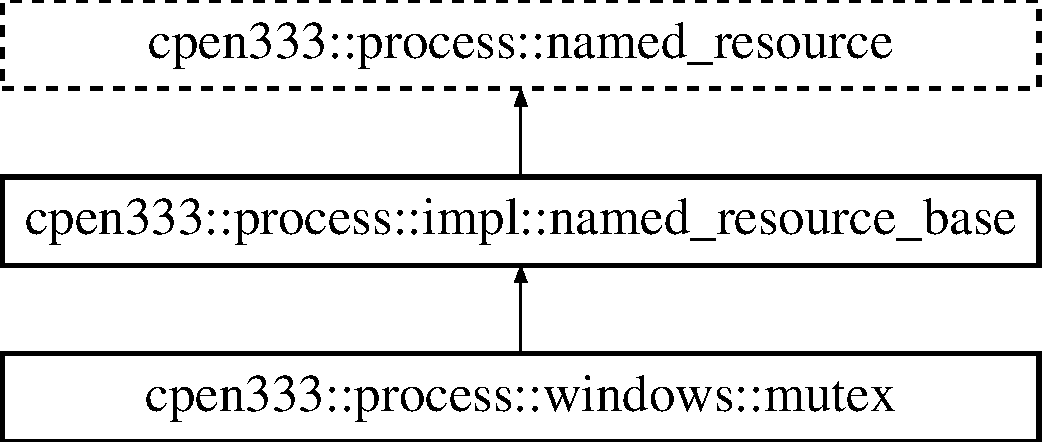
\includegraphics[height=3.000000cm]{classcpen333_1_1process_1_1windows_1_1mutex}
\end{center}
\end{figure}
\subsection*{Public Types}
\begin{DoxyCompactItemize}
\item 
\mbox{\Hypertarget{classcpen333_1_1process_1_1windows_1_1mutex_a6e4acfaa842ca9c60333a33ea613806b}\label{classcpen333_1_1process_1_1windows_1_1mutex_a6e4acfaa842ca9c60333a33ea613806b}} 
using \hyperlink{classcpen333_1_1process_1_1windows_1_1mutex_a6e4acfaa842ca9c60333a33ea613806b}{native\+\_\+handle\+\_\+type} = H\+A\+N\+D\+LE
\begin{DoxyCompactList}\small\item\em Alias to native handle type, which on Windows is type H\+A\+N\+D\+LE. \end{DoxyCompactList}\end{DoxyCompactItemize}
\subsection*{Public Member Functions}
\begin{DoxyCompactItemize}
\item 
\hyperlink{classcpen333_1_1process_1_1windows_1_1mutex_a6bd2d0c07f83dd5646cbdbadbfc8fc58}{mutex} (const std\+::string \&\hyperlink{classcpen333_1_1process_1_1impl_1_1named__resource__base_ae0c5fbb1843afe863cece4b51c38f807}{name})
\begin{DoxyCompactList}\small\item\em Constructs or connects to the named mutex. \end{DoxyCompactList}\item 
\mbox{\Hypertarget{classcpen333_1_1process_1_1windows_1_1mutex_a51a169fed979fd4dcb0a4f9c17cdb99e}\label{classcpen333_1_1process_1_1windows_1_1mutex_a51a169fed979fd4dcb0a4f9c17cdb99e}} 
\hyperlink{classcpen333_1_1process_1_1windows_1_1mutex_a51a169fed979fd4dcb0a4f9c17cdb99e}{$\sim$mutex} ()
\begin{DoxyCompactList}\small\item\em Destructor, closes this instance\textquotesingle{}s handle to the shared mutex. \end{DoxyCompactList}\item 
void \hyperlink{classcpen333_1_1process_1_1windows_1_1mutex_a887f0647207b0e0fa1bead1500c95aec}{lock} ()
\begin{DoxyCompactList}\small\item\em Locks the mutex. \end{DoxyCompactList}\item 
bool \hyperlink{classcpen333_1_1process_1_1windows_1_1mutex_a8fe777a1d576868de91b34d3727132e2}{try\+\_\+lock} ()
\begin{DoxyCompactList}\small\item\em Tries to lock the mutex. \end{DoxyCompactList}\item 
{\footnotesize template$<$class Rep , class Period $>$ }\\bool \hyperlink{classcpen333_1_1process_1_1windows_1_1mutex_aa6a64c60b601c226648cce293835c802}{try\+\_\+lock\+\_\+for} (const std\+::chrono\+::duration$<$ Rep, Period $>$ \&timeout\+\_\+duration)
\begin{DoxyCompactList}\small\item\em Tries to lock the mutex until a relative time has elapsed. \end{DoxyCompactList}\item 
{\footnotesize template$<$class Clock , class Duration $>$ }\\bool \hyperlink{classcpen333_1_1process_1_1windows_1_1mutex_a87d22d9dce4211d0e077cbf7db462fdf}{try\+\_\+lock\+\_\+until} (const std\+::chrono\+::time\+\_\+point$<$ Clock, Duration $>$ \&timeout\+\_\+time)
\begin{DoxyCompactList}\small\item\em Tries to lock the mutex until an absolute time has passed. \end{DoxyCompactList}\item 
bool \hyperlink{classcpen333_1_1process_1_1windows_1_1mutex_a998f0f3d2e56d3acf63a30b465e153a7}{unlock} ()
\begin{DoxyCompactList}\small\item\em Unlocks the mutex. \end{DoxyCompactList}\item 
\hyperlink{classcpen333_1_1process_1_1windows_1_1mutex_a6e4acfaa842ca9c60333a33ea613806b}{native\+\_\+handle\+\_\+type} \hyperlink{classcpen333_1_1process_1_1windows_1_1mutex_a44a60d5a4d372684c8278e7a1f952fb6}{native\+\_\+handle} ()
\begin{DoxyCompactList}\small\item\em Returns a native handle. \end{DoxyCompactList}\item 
bool \hyperlink{classcpen333_1_1process_1_1windows_1_1mutex_aa45381a0a226fbefc86eef8971a5431b}{unlink} ()
\begin{DoxyCompactList}\small\item\em Detaches the name from the named resource. \end{DoxyCompactList}\end{DoxyCompactItemize}
\subsection*{Static Public Member Functions}
\begin{DoxyCompactItemize}
\item 
static bool \hyperlink{classcpen333_1_1process_1_1windows_1_1mutex_aa5a57e9c9c3fdb82bc69c8d1c68ddbfd}{unlink} (const std\+::string \&\hyperlink{classcpen333_1_1process_1_1impl_1_1named__resource__base_ae0c5fbb1843afe863cece4b51c38f807}{name})
\begin{DoxyCompactList}\small\item\em Unlinks the name without needing to create a resource. \end{DoxyCompactList}\end{DoxyCompactItemize}
\subsection*{Additional Inherited Members}


\subsection{Detailed Description}
Inter-\/process named mutual exclusion primitive. 

Used to limit resource access to one thread at a time

This mutex has U\+S\+A\+GE P\+E\+R\+S\+I\+S\+T\+E\+N\+CE, meaning the mutex will continue to exist as long as at least one process/thread is holding a reference to it. 

\subsection{Constructor \& Destructor Documentation}
\mbox{\Hypertarget{classcpen333_1_1process_1_1windows_1_1mutex_a6bd2d0c07f83dd5646cbdbadbfc8fc58}\label{classcpen333_1_1process_1_1windows_1_1mutex_a6bd2d0c07f83dd5646cbdbadbfc8fc58}} 
\index{cpen333\+::process\+::windows\+::mutex@{cpen333\+::process\+::windows\+::mutex}!mutex@{mutex}}
\index{mutex@{mutex}!cpen333\+::process\+::windows\+::mutex@{cpen333\+::process\+::windows\+::mutex}}
\subsubsection{\texorpdfstring{mutex()}{mutex()}}
{\footnotesize\ttfamily cpen333\+::process\+::windows\+::mutex\+::mutex (\begin{DoxyParamCaption}\item[{const std\+::string \&}]{name }\end{DoxyParamCaption})\hspace{0.3cm}{\ttfamily [inline]}}



Constructs or connects to the named mutex. 


\begin{DoxyParams}{Parameters}
{\em name} & identifier for creating or connecting to an existing inter-\/process mutex \\
\hline
\end{DoxyParams}


\subsection{Member Function Documentation}
\mbox{\Hypertarget{classcpen333_1_1process_1_1windows_1_1mutex_a887f0647207b0e0fa1bead1500c95aec}\label{classcpen333_1_1process_1_1windows_1_1mutex_a887f0647207b0e0fa1bead1500c95aec}} 
\index{cpen333\+::process\+::windows\+::mutex@{cpen333\+::process\+::windows\+::mutex}!lock@{lock}}
\index{lock@{lock}!cpen333\+::process\+::windows\+::mutex@{cpen333\+::process\+::windows\+::mutex}}
\subsubsection{\texorpdfstring{lock()}{lock()}}
{\footnotesize\ttfamily void cpen333\+::process\+::windows\+::mutex\+::lock (\begin{DoxyParamCaption}{ }\end{DoxyParamCaption})\hspace{0.3cm}{\ttfamily [inline]}}



Locks the mutex. 

This will block the current thread until the mutex is available to be locked, preventing multiple threads from accessing a protected resource. \mbox{\Hypertarget{classcpen333_1_1process_1_1windows_1_1mutex_a44a60d5a4d372684c8278e7a1f952fb6}\label{classcpen333_1_1process_1_1windows_1_1mutex_a44a60d5a4d372684c8278e7a1f952fb6}} 
\index{cpen333\+::process\+::windows\+::mutex@{cpen333\+::process\+::windows\+::mutex}!native\+\_\+handle@{native\+\_\+handle}}
\index{native\+\_\+handle@{native\+\_\+handle}!cpen333\+::process\+::windows\+::mutex@{cpen333\+::process\+::windows\+::mutex}}
\subsubsection{\texorpdfstring{native\+\_\+handle()}{native\_handle()}}
{\footnotesize\ttfamily \hyperlink{classcpen333_1_1process_1_1windows_1_1mutex_a6e4acfaa842ca9c60333a33ea613806b}{native\+\_\+handle\+\_\+type} cpen333\+::process\+::windows\+::mutex\+::native\+\_\+handle (\begin{DoxyParamCaption}{ }\end{DoxyParamCaption})\hspace{0.3cm}{\ttfamily [inline]}}



Returns a native handle. 

In this case, a Windows H\+A\+N\+D\+LE to the Mutex

\begin{DoxyReturn}{Returns}
native handle to underlying mutex 
\end{DoxyReturn}
\mbox{\Hypertarget{classcpen333_1_1process_1_1windows_1_1mutex_a8fe777a1d576868de91b34d3727132e2}\label{classcpen333_1_1process_1_1windows_1_1mutex_a8fe777a1d576868de91b34d3727132e2}} 
\index{cpen333\+::process\+::windows\+::mutex@{cpen333\+::process\+::windows\+::mutex}!try\+\_\+lock@{try\+\_\+lock}}
\index{try\+\_\+lock@{try\+\_\+lock}!cpen333\+::process\+::windows\+::mutex@{cpen333\+::process\+::windows\+::mutex}}
\subsubsection{\texorpdfstring{try\+\_\+lock()}{try\_lock()}}
{\footnotesize\ttfamily bool cpen333\+::process\+::windows\+::mutex\+::try\+\_\+lock (\begin{DoxyParamCaption}{ }\end{DoxyParamCaption})\hspace{0.3cm}{\ttfamily [inline]}}



Tries to lock the mutex. 

This will attempt to lock the mutex, returning immediately.

\begin{DoxyReturn}{Returns}
true if locked successfully, false if already locked 
\end{DoxyReturn}
\mbox{\Hypertarget{classcpen333_1_1process_1_1windows_1_1mutex_aa6a64c60b601c226648cce293835c802}\label{classcpen333_1_1process_1_1windows_1_1mutex_aa6a64c60b601c226648cce293835c802}} 
\index{cpen333\+::process\+::windows\+::mutex@{cpen333\+::process\+::windows\+::mutex}!try\+\_\+lock\+\_\+for@{try\+\_\+lock\+\_\+for}}
\index{try\+\_\+lock\+\_\+for@{try\+\_\+lock\+\_\+for}!cpen333\+::process\+::windows\+::mutex@{cpen333\+::process\+::windows\+::mutex}}
\subsubsection{\texorpdfstring{try\+\_\+lock\+\_\+for()}{try\_lock\_for()}}
{\footnotesize\ttfamily template$<$class Rep , class Period $>$ \\
bool cpen333\+::process\+::windows\+::mutex\+::try\+\_\+lock\+\_\+for (\begin{DoxyParamCaption}\item[{const std\+::chrono\+::duration$<$ Rep, Period $>$ \&}]{timeout\+\_\+duration }\end{DoxyParamCaption})\hspace{0.3cm}{\ttfamily [inline]}}



Tries to lock the mutex until a relative time has elapsed. 

Blocks until the specified timeout duration has elapsed or the lock is acquired, whichever comes first.


\begin{DoxyTemplParams}{Template Parameters}
{\em Rep} & timer representation \\
\hline
{\em Period} & timeout period type \\
\hline
\end{DoxyTemplParams}

\begin{DoxyParams}{Parameters}
{\em timeout\+\_\+duration} & maximum relative time to block for \\
\hline
\end{DoxyParams}
\begin{DoxyReturn}{Returns}
true if lock was acquired successfully, false otherwise 
\end{DoxyReturn}
\mbox{\Hypertarget{classcpen333_1_1process_1_1windows_1_1mutex_a87d22d9dce4211d0e077cbf7db462fdf}\label{classcpen333_1_1process_1_1windows_1_1mutex_a87d22d9dce4211d0e077cbf7db462fdf}} 
\index{cpen333\+::process\+::windows\+::mutex@{cpen333\+::process\+::windows\+::mutex}!try\+\_\+lock\+\_\+until@{try\+\_\+lock\+\_\+until}}
\index{try\+\_\+lock\+\_\+until@{try\+\_\+lock\+\_\+until}!cpen333\+::process\+::windows\+::mutex@{cpen333\+::process\+::windows\+::mutex}}
\subsubsection{\texorpdfstring{try\+\_\+lock\+\_\+until()}{try\_lock\_until()}}
{\footnotesize\ttfamily template$<$class Clock , class Duration $>$ \\
bool cpen333\+::process\+::windows\+::mutex\+::try\+\_\+lock\+\_\+until (\begin{DoxyParamCaption}\item[{const std\+::chrono\+::time\+\_\+point$<$ Clock, Duration $>$ \&}]{timeout\+\_\+time }\end{DoxyParamCaption})\hspace{0.3cm}{\ttfamily [inline]}}



Tries to lock the mutex until an absolute time has passed. 


\begin{DoxyTemplParams}{Template Parameters}
{\em Clock} & timeout clock type \\
\hline
{\em Duration} & timeout duration type \\
\hline
\end{DoxyTemplParams}

\begin{DoxyParams}{Parameters}
{\em timeout\+\_\+time} & absolute timeout time \\
\hline
\end{DoxyParams}
\begin{DoxyReturn}{Returns}
true if the lock was acquired successfully, false otherwise 
\end{DoxyReturn}
\mbox{\Hypertarget{classcpen333_1_1process_1_1windows_1_1mutex_aa45381a0a226fbefc86eef8971a5431b}\label{classcpen333_1_1process_1_1windows_1_1mutex_aa45381a0a226fbefc86eef8971a5431b}} 
\index{cpen333\+::process\+::windows\+::mutex@{cpen333\+::process\+::windows\+::mutex}!unlink@{unlink}}
\index{unlink@{unlink}!cpen333\+::process\+::windows\+::mutex@{cpen333\+::process\+::windows\+::mutex}}
\subsubsection{\texorpdfstring{unlink()}{unlink()}\hspace{0.1cm}{\footnotesize\ttfamily [1/2]}}
{\footnotesize\ttfamily bool cpen333\+::process\+::windows\+::mutex\+::unlink (\begin{DoxyParamCaption}{ }\end{DoxyParamCaption})\hspace{0.3cm}{\ttfamily [inline]}, {\ttfamily [virtual]}}



Detaches the name from the named resource. 

On P\+O\+S\+IX systems, named resources will persist beyond the lifetime of any process that uses them as long as the name has not been unlinked (or until the system is rebooted). Calling {\ttfamily unlink} will detach the name, allowing the resource to be freed once all current users have exited.

\begin{DoxyReturn}{Returns}
{\ttfamily true} if unlink is successful, {\ttfamily false} if unlinking is not supported or if an error has occurred. 
\end{DoxyReturn}


Implements \hyperlink{classcpen333_1_1process_1_1impl_1_1named__resource__base_ae4033f82dfd068b917a9bca57d3a0c45}{cpen333\+::process\+::impl\+::named\+\_\+resource\+\_\+base}.

\mbox{\Hypertarget{classcpen333_1_1process_1_1windows_1_1mutex_aa5a57e9c9c3fdb82bc69c8d1c68ddbfd}\label{classcpen333_1_1process_1_1windows_1_1mutex_aa5a57e9c9c3fdb82bc69c8d1c68ddbfd}} 
\index{cpen333\+::process\+::windows\+::mutex@{cpen333\+::process\+::windows\+::mutex}!unlink@{unlink}}
\index{unlink@{unlink}!cpen333\+::process\+::windows\+::mutex@{cpen333\+::process\+::windows\+::mutex}}
\subsubsection{\texorpdfstring{unlink()}{unlink()}\hspace{0.1cm}{\footnotesize\ttfamily [2/2]}}
{\footnotesize\ttfamily static bool cpen333\+::process\+::windows\+::mutex\+::unlink (\begin{DoxyParamCaption}\item[{const std\+::string \&}]{name }\end{DoxyParamCaption})\hspace{0.3cm}{\ttfamily [inline]}, {\ttfamily [static]}}



Unlinks the name without needing to create a resource. 

Implementers should also provide a static method for unlinking. The purpose is mainly for clean-\/up of existing resources.


\begin{DoxyParams}{Parameters}
{\em name} & desired resource name \\
\hline
\end{DoxyParams}
\begin{DoxyReturn}{Returns}
{\ttfamily true} if unlink successful, {\ttfamily false} if not successful or not supported 
\end{DoxyReturn}
\mbox{\Hypertarget{classcpen333_1_1process_1_1windows_1_1mutex_a998f0f3d2e56d3acf63a30b465e153a7}\label{classcpen333_1_1process_1_1windows_1_1mutex_a998f0f3d2e56d3acf63a30b465e153a7}} 
\index{cpen333\+::process\+::windows\+::mutex@{cpen333\+::process\+::windows\+::mutex}!unlock@{unlock}}
\index{unlock@{unlock}!cpen333\+::process\+::windows\+::mutex@{cpen333\+::process\+::windows\+::mutex}}
\subsubsection{\texorpdfstring{unlock()}{unlock()}}
{\footnotesize\ttfamily bool cpen333\+::process\+::windows\+::mutex\+::unlock (\begin{DoxyParamCaption}{ }\end{DoxyParamCaption})\hspace{0.3cm}{\ttfamily [inline]}}



Unlocks the mutex. 

Puts the mutex in a state to be relocked, freeing the protected resource to be used by another (or the same) thread 

The documentation for this class was generated from the following file\+:\begin{DoxyCompactItemize}
\item 
D\+:/school/teaching/\+C\+P\+E\+N333/workspace/labs/include/cpen333/process/impl/windows/\hyperlink{impl_2windows_2mutex_8h}{mutex.\+h}\end{DoxyCompactItemize}

\hypertarget{classcpen333_1_1process_1_1mutex}{}\section{cpen333\+:\+:process\+:\+:mutex Class Reference}
\label{classcpen333_1_1process_1_1mutex}\index{cpen333\+::process\+::mutex@{cpen333\+::process\+::mutex}}


An inter-\/process mutual exclusion synchronization primitive.  




{\ttfamily \#include $<$mutex.\+h$>$}



\subsection{Detailed Description}
An inter-\/process mutual exclusion synchronization primitive. 

Used to protect access to a resource shared by multiple processes. This is an alias to either \hyperlink{classcpen333_1_1process_1_1posix_1_1mutex}{cpen333\+::process\+::posix\+::mutex} or \hyperlink{classcpen333_1_1process_1_1windows_1_1mutex}{cpen333\+::process\+::windows\+::mutex} depending on your platform. 

The documentation for this class was generated from the following file\+:\begin{DoxyCompactItemize}
\item 
D\+:/school/teaching/\+C\+P\+E\+N333/workspace/labs/include/cpen333/process/\hyperlink{mutex_8h}{mutex.\+h}\end{DoxyCompactItemize}

\hypertarget{classcpen333_1_1process_1_1posix_1_1mutex}{}\section{cpen333\+:\+:process\+:\+:posix\+:\+:mutex Class Reference}
\label{classcpen333_1_1process_1_1posix_1_1mutex}\index{cpen333\+::process\+::posix\+::mutex@{cpen333\+::process\+::posix\+::mutex}}


Inter-\/process named mutual exclusion primitive.  




{\ttfamily \#include $<$mutex.\+h$>$}

Inheritance diagram for cpen333\+:\+:process\+:\+:posix\+:\+:mutex\+:\begin{figure}[H]
\begin{center}
\leavevmode
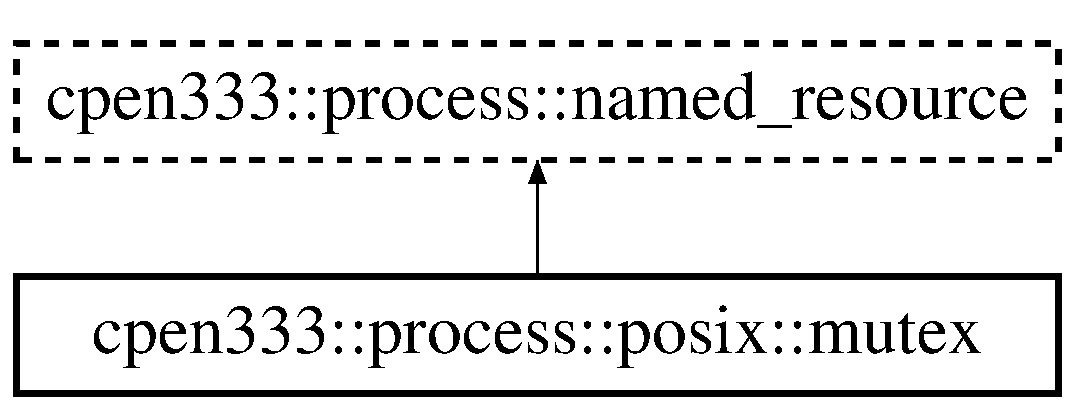
\includegraphics[height=2.000000cm]{classcpen333_1_1process_1_1posix_1_1mutex}
\end{center}
\end{figure}
\subsection*{Public Types}
\begin{DoxyCompactItemize}
\item 
\mbox{\Hypertarget{classcpen333_1_1process_1_1posix_1_1mutex_aac6d3675fcffc52ddf281e952968e44b}\label{classcpen333_1_1process_1_1posix_1_1mutex_aac6d3675fcffc52ddf281e952968e44b}} 
using \hyperlink{classcpen333_1_1process_1_1posix_1_1mutex_aac6d3675fcffc52ddf281e952968e44b}{native\+\_\+handle\+\_\+type} = \hyperlink{classcpen333_1_1process_1_1posix_1_1semaphore_ad63150e5c8c196a84a7b214462756f1a}{semaphore\+::native\+\_\+handle\+\_\+type}
\begin{DoxyCompactList}\small\item\em Alias to the underlying native mutex handle. \end{DoxyCompactList}\end{DoxyCompactItemize}
\subsection*{Public Member Functions}
\begin{DoxyCompactItemize}
\item 
\hyperlink{classcpen333_1_1process_1_1posix_1_1mutex_a72ecaf79b2e4ea585b542dc0ed240614}{mutex} (const std\+::string \&name)
\begin{DoxyCompactList}\small\item\em Constructs or connects to the named mutex. \end{DoxyCompactList}\item 
void \hyperlink{classcpen333_1_1process_1_1posix_1_1mutex_a07dccda80dc88292fa490ce47dd0faa6}{lock} ()
\begin{DoxyCompactList}\small\item\em Locks the mutex. \end{DoxyCompactList}\item 
bool \hyperlink{classcpen333_1_1process_1_1posix_1_1mutex_ae19f7c8370308f7333cee340fef91049}{try\+\_\+lock} ()
\begin{DoxyCompactList}\small\item\em Tries to lock the mutex. \end{DoxyCompactList}\item 
{\footnotesize template$<$class Rep , class Period $>$ }\\bool \hyperlink{classcpen333_1_1process_1_1posix_1_1mutex_a28ac1db650efaae2d959df0e555f3d24}{try\+\_\+lock\+\_\+for} (const std\+::chrono\+::duration$<$ Rep, Period $>$ \&timeout\+\_\+duration)
\begin{DoxyCompactList}\small\item\em Tries to lock the mutex until a relative time has elapsed. \end{DoxyCompactList}\item 
{\footnotesize template$<$class Clock , class Duration $>$ }\\bool \hyperlink{classcpen333_1_1process_1_1posix_1_1mutex_a0cfd76098d89d269ad4a89115e7673d1}{try\+\_\+lock\+\_\+until} (const std\+::chrono\+::time\+\_\+point$<$ Clock, Duration $>$ \&timeout\+\_\+time)
\begin{DoxyCompactList}\small\item\em Tries to lock the mutex until an absolute time has passed. \end{DoxyCompactList}\item 
void \hyperlink{classcpen333_1_1process_1_1posix_1_1mutex_a822e51a57ea9e5de1a052aeddf3e4e02}{unlock} ()
\begin{DoxyCompactList}\small\item\em Unlocks the mutex. \end{DoxyCompactList}\item 
\hyperlink{classcpen333_1_1process_1_1posix_1_1mutex_aac6d3675fcffc52ddf281e952968e44b}{native\+\_\+handle\+\_\+type} \hyperlink{classcpen333_1_1process_1_1posix_1_1mutex_aa36462cbd2181e20caa35656c619c6dd}{native\+\_\+handle} ()
\begin{DoxyCompactList}\small\item\em Returns a native handle. \end{DoxyCompactList}\item 
bool \hyperlink{classcpen333_1_1process_1_1posix_1_1mutex_ac1bcf9576d7470e5d64e17876c9cdb36}{unlink} ()
\begin{DoxyCompactList}\small\item\em Detaches the name from the named resource. \end{DoxyCompactList}\end{DoxyCompactItemize}
\subsection*{Static Public Member Functions}
\begin{DoxyCompactItemize}
\item 
static bool \hyperlink{classcpen333_1_1process_1_1posix_1_1mutex_ae5750c148e0408daac498a87d2d9a579}{unlink} (const std\+::string \&name)
\begin{DoxyCompactList}\small\item\em Unlinks the name without needing to create a resource. \end{DoxyCompactList}\end{DoxyCompactItemize}


\subsection{Detailed Description}
Inter-\/process named mutual exclusion primitive. 

Used to limit resource access to one thread at a time

Based on a named semaphore. Unlike a true mutex, this implementation does N\+OT enforce that the same thread unlock the mutex. However, in practice, it should be treated as a true mutex by using std\+::lock\+\_\+guard or std\+::unique\+\_\+lock.

This mutex has K\+E\+R\+N\+EL P\+E\+R\+S\+I\+S\+T\+E\+N\+CE, meaning if not \hyperlink{classcpen333_1_1process_1_1posix_1_1mutex_ac1bcf9576d7470e5d64e17876c9cdb36}{unlink()}-\/ed, will continue to exist in its current state until the system is shut down (persisting beyond the life of the initiating program) 

\subsection{Constructor \& Destructor Documentation}
\mbox{\Hypertarget{classcpen333_1_1process_1_1posix_1_1mutex_a72ecaf79b2e4ea585b542dc0ed240614}\label{classcpen333_1_1process_1_1posix_1_1mutex_a72ecaf79b2e4ea585b542dc0ed240614}} 
\index{cpen333\+::process\+::posix\+::mutex@{cpen333\+::process\+::posix\+::mutex}!mutex@{mutex}}
\index{mutex@{mutex}!cpen333\+::process\+::posix\+::mutex@{cpen333\+::process\+::posix\+::mutex}}
\subsubsection{\texorpdfstring{mutex()}{mutex()}}
{\footnotesize\ttfamily cpen333\+::process\+::posix\+::mutex\+::mutex (\begin{DoxyParamCaption}\item[{const std\+::string \&}]{name }\end{DoxyParamCaption})\hspace{0.3cm}{\ttfamily [inline]}}



Constructs or connects to the named mutex. 


\begin{DoxyParams}{Parameters}
{\em name} & identifier for creating or connecting to an existing inter-\/process mutex \\
\hline
\end{DoxyParams}


\subsection{Member Function Documentation}
\mbox{\Hypertarget{classcpen333_1_1process_1_1posix_1_1mutex_a07dccda80dc88292fa490ce47dd0faa6}\label{classcpen333_1_1process_1_1posix_1_1mutex_a07dccda80dc88292fa490ce47dd0faa6}} 
\index{cpen333\+::process\+::posix\+::mutex@{cpen333\+::process\+::posix\+::mutex}!lock@{lock}}
\index{lock@{lock}!cpen333\+::process\+::posix\+::mutex@{cpen333\+::process\+::posix\+::mutex}}
\subsubsection{\texorpdfstring{lock()}{lock()}}
{\footnotesize\ttfamily void cpen333\+::process\+::posix\+::mutex\+::lock (\begin{DoxyParamCaption}{ }\end{DoxyParamCaption})\hspace{0.3cm}{\ttfamily [inline]}}



Locks the mutex. 

This will block the current thread until the mutex is available to be locked, preventing multiple threads from accessing a protected resource. \mbox{\Hypertarget{classcpen333_1_1process_1_1posix_1_1mutex_aa36462cbd2181e20caa35656c619c6dd}\label{classcpen333_1_1process_1_1posix_1_1mutex_aa36462cbd2181e20caa35656c619c6dd}} 
\index{cpen333\+::process\+::posix\+::mutex@{cpen333\+::process\+::posix\+::mutex}!native\+\_\+handle@{native\+\_\+handle}}
\index{native\+\_\+handle@{native\+\_\+handle}!cpen333\+::process\+::posix\+::mutex@{cpen333\+::process\+::posix\+::mutex}}
\subsubsection{\texorpdfstring{native\+\_\+handle()}{native\_handle()}}
{\footnotesize\ttfamily \hyperlink{classcpen333_1_1process_1_1posix_1_1mutex_aac6d3675fcffc52ddf281e952968e44b}{native\+\_\+handle\+\_\+type} cpen333\+::process\+::posix\+::mutex\+::native\+\_\+handle (\begin{DoxyParamCaption}{ }\end{DoxyParamCaption})\hspace{0.3cm}{\ttfamily [inline]}}



Returns a native handle. 

In this case, a P\+O\+S\+IX sem\+\_\+t

\begin{DoxyReturn}{Returns}
native handle to underlying mutex 
\end{DoxyReturn}
\mbox{\Hypertarget{classcpen333_1_1process_1_1posix_1_1mutex_ae19f7c8370308f7333cee340fef91049}\label{classcpen333_1_1process_1_1posix_1_1mutex_ae19f7c8370308f7333cee340fef91049}} 
\index{cpen333\+::process\+::posix\+::mutex@{cpen333\+::process\+::posix\+::mutex}!try\+\_\+lock@{try\+\_\+lock}}
\index{try\+\_\+lock@{try\+\_\+lock}!cpen333\+::process\+::posix\+::mutex@{cpen333\+::process\+::posix\+::mutex}}
\subsubsection{\texorpdfstring{try\+\_\+lock()}{try\_lock()}}
{\footnotesize\ttfamily bool cpen333\+::process\+::posix\+::mutex\+::try\+\_\+lock (\begin{DoxyParamCaption}{ }\end{DoxyParamCaption})\hspace{0.3cm}{\ttfamily [inline]}}



Tries to lock the mutex. 

This will attempt to lock the mutex, returning immediately.

\begin{DoxyReturn}{Returns}
true if locked successfully, false if already locked 
\end{DoxyReturn}
\mbox{\Hypertarget{classcpen333_1_1process_1_1posix_1_1mutex_a28ac1db650efaae2d959df0e555f3d24}\label{classcpen333_1_1process_1_1posix_1_1mutex_a28ac1db650efaae2d959df0e555f3d24}} 
\index{cpen333\+::process\+::posix\+::mutex@{cpen333\+::process\+::posix\+::mutex}!try\+\_\+lock\+\_\+for@{try\+\_\+lock\+\_\+for}}
\index{try\+\_\+lock\+\_\+for@{try\+\_\+lock\+\_\+for}!cpen333\+::process\+::posix\+::mutex@{cpen333\+::process\+::posix\+::mutex}}
\subsubsection{\texorpdfstring{try\+\_\+lock\+\_\+for()}{try\_lock\_for()}}
{\footnotesize\ttfamily template$<$class Rep , class Period $>$ \\
bool cpen333\+::process\+::posix\+::mutex\+::try\+\_\+lock\+\_\+for (\begin{DoxyParamCaption}\item[{const std\+::chrono\+::duration$<$ Rep, Period $>$ \&}]{timeout\+\_\+duration }\end{DoxyParamCaption})\hspace{0.3cm}{\ttfamily [inline]}}



Tries to lock the mutex until a relative time has elapsed. 

Blocks until the specified timeout duration has elapsed or the lock is acquired, whichever comes first.


\begin{DoxyTemplParams}{Template Parameters}
{\em Rep} & timer representation \\
\hline
{\em Period} & timeout period type \\
\hline
\end{DoxyTemplParams}

\begin{DoxyParams}{Parameters}
{\em timeout\+\_\+duration} & maximum relative time to block for \\
\hline
\end{DoxyParams}
\begin{DoxyReturn}{Returns}
true if lock was acquired successfully, false otherwise 
\end{DoxyReturn}
\mbox{\Hypertarget{classcpen333_1_1process_1_1posix_1_1mutex_a0cfd76098d89d269ad4a89115e7673d1}\label{classcpen333_1_1process_1_1posix_1_1mutex_a0cfd76098d89d269ad4a89115e7673d1}} 
\index{cpen333\+::process\+::posix\+::mutex@{cpen333\+::process\+::posix\+::mutex}!try\+\_\+lock\+\_\+until@{try\+\_\+lock\+\_\+until}}
\index{try\+\_\+lock\+\_\+until@{try\+\_\+lock\+\_\+until}!cpen333\+::process\+::posix\+::mutex@{cpen333\+::process\+::posix\+::mutex}}
\subsubsection{\texorpdfstring{try\+\_\+lock\+\_\+until()}{try\_lock\_until()}}
{\footnotesize\ttfamily template$<$class Clock , class Duration $>$ \\
bool cpen333\+::process\+::posix\+::mutex\+::try\+\_\+lock\+\_\+until (\begin{DoxyParamCaption}\item[{const std\+::chrono\+::time\+\_\+point$<$ Clock, Duration $>$ \&}]{timeout\+\_\+time }\end{DoxyParamCaption})\hspace{0.3cm}{\ttfamily [inline]}}



Tries to lock the mutex until an absolute time has passed. 


\begin{DoxyTemplParams}{Template Parameters}
{\em Clock} & timeout clock type \\
\hline
{\em Duration} & timeout duration type \\
\hline
\end{DoxyTemplParams}

\begin{DoxyParams}{Parameters}
{\em timeout\+\_\+time} & absolute timeout time \\
\hline
\end{DoxyParams}
\begin{DoxyReturn}{Returns}
true if the lock was acquired successfully, false otherwise 
\end{DoxyReturn}
\mbox{\Hypertarget{classcpen333_1_1process_1_1posix_1_1mutex_ac1bcf9576d7470e5d64e17876c9cdb36}\label{classcpen333_1_1process_1_1posix_1_1mutex_ac1bcf9576d7470e5d64e17876c9cdb36}} 
\index{cpen333\+::process\+::posix\+::mutex@{cpen333\+::process\+::posix\+::mutex}!unlink@{unlink}}
\index{unlink@{unlink}!cpen333\+::process\+::posix\+::mutex@{cpen333\+::process\+::posix\+::mutex}}
\subsubsection{\texorpdfstring{unlink()}{unlink()}\hspace{0.1cm}{\footnotesize\ttfamily [1/2]}}
{\footnotesize\ttfamily bool cpen333\+::process\+::posix\+::mutex\+::unlink (\begin{DoxyParamCaption}{ }\end{DoxyParamCaption})\hspace{0.3cm}{\ttfamily [inline]}, {\ttfamily [virtual]}}



Detaches the name from the named resource. 

On P\+O\+S\+IX systems, named resources will persist beyond the lifetime of any process that uses them as long as the name has not been unlinked (or until the system is rebooted). Calling {\ttfamily unlink} will detach the name, allowing the resource to be freed once all current users have exited.

\begin{DoxyReturn}{Returns}
{\ttfamily true} if unlink is successful, {\ttfamily false} if unlinking is not supported or if an error has occurred. 
\end{DoxyReturn}


Implements \hyperlink{classcpen333_1_1process_1_1named__resource_a5d33168fee48c9b0c58ab8fd96e230ce}{cpen333\+::process\+::named\+\_\+resource}.

\mbox{\Hypertarget{classcpen333_1_1process_1_1posix_1_1mutex_ae5750c148e0408daac498a87d2d9a579}\label{classcpen333_1_1process_1_1posix_1_1mutex_ae5750c148e0408daac498a87d2d9a579}} 
\index{cpen333\+::process\+::posix\+::mutex@{cpen333\+::process\+::posix\+::mutex}!unlink@{unlink}}
\index{unlink@{unlink}!cpen333\+::process\+::posix\+::mutex@{cpen333\+::process\+::posix\+::mutex}}
\subsubsection{\texorpdfstring{unlink()}{unlink()}\hspace{0.1cm}{\footnotesize\ttfamily [2/2]}}
{\footnotesize\ttfamily static bool cpen333\+::process\+::posix\+::mutex\+::unlink (\begin{DoxyParamCaption}\item[{const std\+::string \&}]{name }\end{DoxyParamCaption})\hspace{0.3cm}{\ttfamily [inline]}, {\ttfamily [static]}}



Unlinks the name without needing to create a resource. 

Implementers should also provide a static method for unlinking. The purpose is mainly for clean-\/up of existing resources.


\begin{DoxyParams}{Parameters}
{\em name} & desired resource name \\
\hline
\end{DoxyParams}
\begin{DoxyReturn}{Returns}
{\ttfamily true} if unlink successful, {\ttfamily false} if not successful or not supported 
\end{DoxyReturn}
\mbox{\Hypertarget{classcpen333_1_1process_1_1posix_1_1mutex_a822e51a57ea9e5de1a052aeddf3e4e02}\label{classcpen333_1_1process_1_1posix_1_1mutex_a822e51a57ea9e5de1a052aeddf3e4e02}} 
\index{cpen333\+::process\+::posix\+::mutex@{cpen333\+::process\+::posix\+::mutex}!unlock@{unlock}}
\index{unlock@{unlock}!cpen333\+::process\+::posix\+::mutex@{cpen333\+::process\+::posix\+::mutex}}
\subsubsection{\texorpdfstring{unlock()}{unlock()}}
{\footnotesize\ttfamily void cpen333\+::process\+::posix\+::mutex\+::unlock (\begin{DoxyParamCaption}{ }\end{DoxyParamCaption})\hspace{0.3cm}{\ttfamily [inline]}}



Unlocks the mutex. 

Puts the mutex in a state to be relocked, freeing the protected resource to be used by another (or the same) thread 

The documentation for this class was generated from the following file\+:\begin{DoxyCompactItemize}
\item 
D\+:/school/teaching/\+C\+P\+E\+N333/workspace/labs/include/cpen333/process/impl/posix/\hyperlink{impl_2posix_2mutex_8h}{mutex.\+h}\end{DoxyCompactItemize}

\hypertarget{classcpen333_1_1process_1_1named__resource}{}\section{cpen333\+:\+:process\+:\+:named\+\_\+resource Class Reference}
\label{classcpen333_1_1process_1_1named__resource}\index{cpen333\+::process\+::named\+\_\+resource@{cpen333\+::process\+::named\+\_\+resource}}


Pure virtual base class for all inter-\/process resources.  




{\ttfamily \#include $<$named\+\_\+resource.\+h$>$}

Inheritance diagram for cpen333\+:\+:process\+:\+:named\+\_\+resource\+:\begin{figure}[H]
\begin{center}
\leavevmode
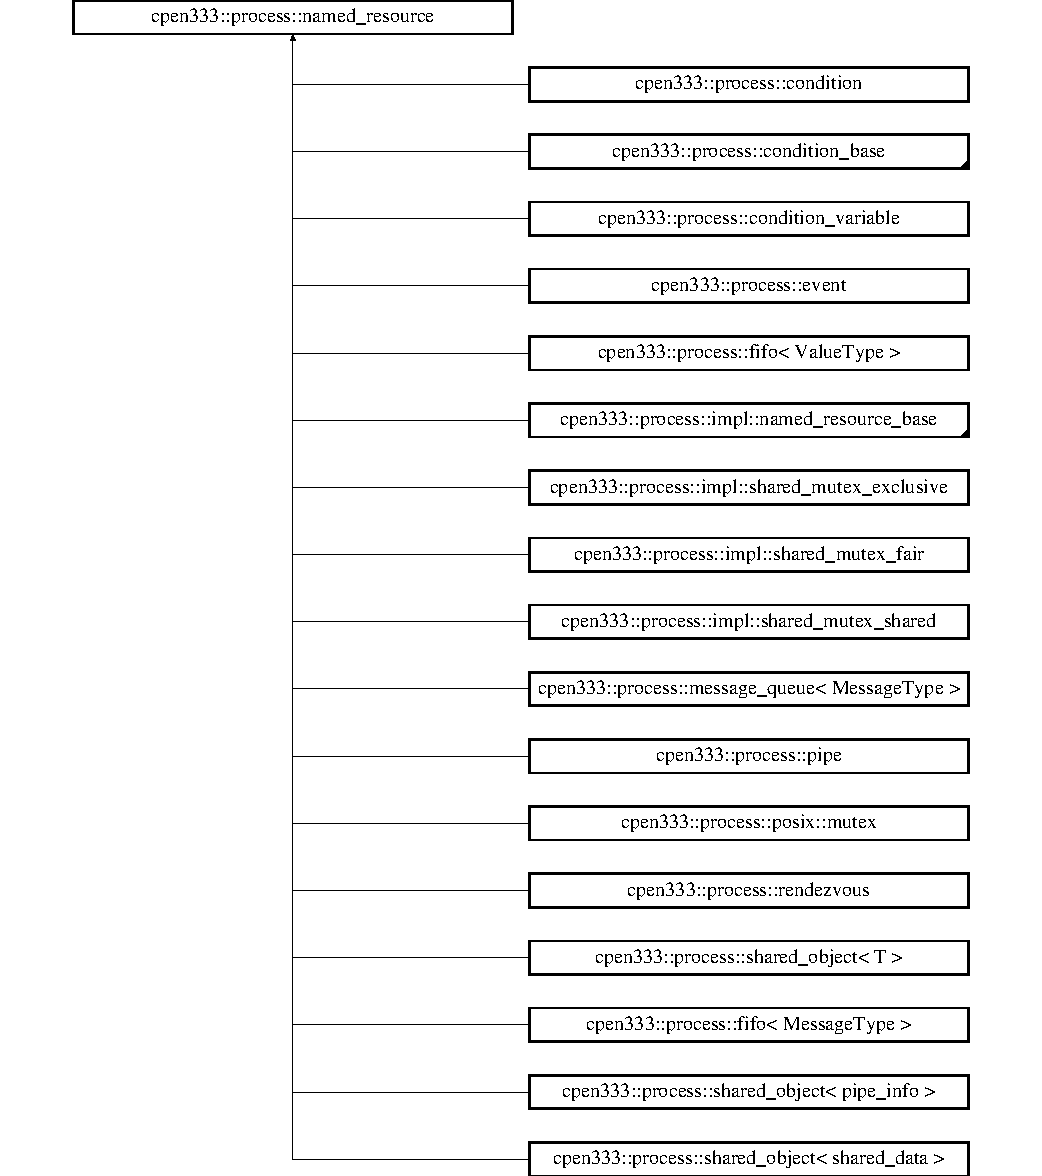
\includegraphics[height=12.000000cm]{classcpen333_1_1process_1_1named__resource}
\end{center}
\end{figure}
\subsection*{Public Member Functions}
\begin{DoxyCompactItemize}
\item 
\mbox{\Hypertarget{classcpen333_1_1process_1_1named__resource_a2bf88d9fa295c5e9ffecf2a43414e6da}\label{classcpen333_1_1process_1_1named__resource_a2bf88d9fa295c5e9ffecf2a43414e6da}} 
virtual \hyperlink{classcpen333_1_1process_1_1named__resource_a2bf88d9fa295c5e9ffecf2a43414e6da}{$\sim$named\+\_\+resource} ()
\begin{DoxyCompactList}\small\item\em Virtual destructor. \end{DoxyCompactList}\item 
virtual bool \hyperlink{classcpen333_1_1process_1_1named__resource_a5d33168fee48c9b0c58ab8fd96e230ce}{unlink} ()=0
\begin{DoxyCompactList}\small\item\em Detaches the name from the named resource. \end{DoxyCompactList}\end{DoxyCompactItemize}
\subsection*{Static Public Member Functions}
\begin{DoxyCompactItemize}
\item 
static bool \hyperlink{classcpen333_1_1process_1_1named__resource_a6cb427f033b51f08fcf2bc1e08bd6a32}{unlink} (const std\+::string \&name)
\begin{DoxyCompactList}\small\item\em Unlinks the name without needing to create a resource. \end{DoxyCompactList}\end{DoxyCompactItemize}


\subsection{Detailed Description}
Pure virtual base class for all inter-\/process resources. 

Named resources are accessed using an identifying name during construction. If the name and resource exists, it will connecting to the existing version. Otherwise, a new resource will be allocated. The resource will persist as long as processes are using it.

On P\+O\+S\+IX systems, a named resource has kernel persistence, meaning it will continue to exist until either the name is manually \char`\"{}unlinked\char`\"{} from the resource, or until the next reboot. If unlinked, the name is detached from the resource, but the resource will continue to exist and be accessible until all current users have finished using it. If any new users try to access the resource with the previous unlinked name, it will be viewed as a new usage, and a new separate resource will be allocated.

On Windows, the named resource will persist until all users have released it. There is not concept of \char`\"{}unlinking\char`\"{} in Windows. 

\subsection{Member Function Documentation}
\mbox{\Hypertarget{classcpen333_1_1process_1_1named__resource_a5d33168fee48c9b0c58ab8fd96e230ce}\label{classcpen333_1_1process_1_1named__resource_a5d33168fee48c9b0c58ab8fd96e230ce}} 
\index{cpen333\+::process\+::named\+\_\+resource@{cpen333\+::process\+::named\+\_\+resource}!unlink@{unlink}}
\index{unlink@{unlink}!cpen333\+::process\+::named\+\_\+resource@{cpen333\+::process\+::named\+\_\+resource}}
\subsubsection{\texorpdfstring{unlink()}{unlink()}\hspace{0.1cm}{\footnotesize\ttfamily [1/2]}}
{\footnotesize\ttfamily virtual bool cpen333\+::process\+::named\+\_\+resource\+::unlink (\begin{DoxyParamCaption}{ }\end{DoxyParamCaption})\hspace{0.3cm}{\ttfamily [pure virtual]}}



Detaches the name from the named resource. 

On P\+O\+S\+IX systems, named resources will persist beyond the lifetime of any process that uses them as long as the name has not been unlinked (or until the system is rebooted). Calling {\ttfamily unlink} will detach the name, allowing the resource to be freed once all current users have exited.

\begin{DoxyReturn}{Returns}
{\ttfamily true} if unlink is successful, {\ttfamily false} if unlinking is not supported or if an error has occurred. 
\end{DoxyReturn}


Implemented in \hyperlink{classcpen333_1_1process_1_1pipe_addcc650694ad0712637874eb79ec8407}{cpen333\+::process\+::pipe}, \hyperlink{classcpen333_1_1process_1_1fifo_a85f9c252de8044d57568e99b64cbb860}{cpen333\+::process\+::fifo$<$ Value\+Type $>$}, \hyperlink{classcpen333_1_1process_1_1fifo_a85f9c252de8044d57568e99b64cbb860}{cpen333\+::process\+::fifo$<$ Message\+Type $>$}, \hyperlink{classcpen333_1_1process_1_1impl_1_1shared__mutex__exclusive_ad296e92049cc48cc3c40ec7404bf836c}{cpen333\+::process\+::impl\+::shared\+\_\+mutex\+\_\+exclusive}, \hyperlink{classcpen333_1_1process_1_1message__queue_ae94a6503dff948dfc2533f7786839dca}{cpen333\+::process\+::message\+\_\+queue$<$ Message\+Type $>$}, \hyperlink{classcpen333_1_1process_1_1impl_1_1shared__mutex__fair_a40e20137e0c27f4a742ab6c5388eb61b}{cpen333\+::process\+::impl\+::shared\+\_\+mutex\+\_\+fair}, \hyperlink{classcpen333_1_1process_1_1posix_1_1semaphore_aa6064e2c4b4b7282cc5e6eda877ee1bb}{cpen333\+::process\+::posix\+::semaphore}, \hyperlink{classcpen333_1_1process_1_1condition__variable_a2861ec071acc52be7ca5790edd062ee8}{cpen333\+::process\+::condition\+\_\+variable}, \hyperlink{classcpen333_1_1process_1_1impl_1_1shared__mutex__shared_a8e6c759f5d5266b931ed78da04652d61}{cpen333\+::process\+::impl\+::shared\+\_\+mutex\+\_\+shared}, \hyperlink{classcpen333_1_1process_1_1condition__base_acd6d0b53a828aa161ccad06885eaa15c}{cpen333\+::process\+::condition\+\_\+base}, \hyperlink{classcpen333_1_1process_1_1windows_1_1semaphore_abc5159f32e61024c6c6a978ac64fe39d}{cpen333\+::process\+::windows\+::semaphore}, \hyperlink{classcpen333_1_1process_1_1windows_1_1shared__memory_aa6efdc9a3e1310ea69ecc48aeb41286c}{cpen333\+::process\+::windows\+::shared\+\_\+memory}, \hyperlink{classcpen333_1_1process_1_1condition_a7c646204b2c4912185ba6055c9afa3f6}{cpen333\+::process\+::condition}, \hyperlink{classcpen333_1_1process_1_1posix_1_1mutex_ac1bcf9576d7470e5d64e17876c9cdb36}{cpen333\+::process\+::posix\+::mutex}, \hyperlink{classcpen333_1_1process_1_1windows_1_1mutex_aa45381a0a226fbefc86eef8971a5431b}{cpen333\+::process\+::windows\+::mutex}, \hyperlink{classcpen333_1_1process_1_1posix_1_1shared__memory_a3b6d67a41cfaca3712d87958682d8bbe}{cpen333\+::process\+::posix\+::shared\+\_\+memory}, \hyperlink{classcpen333_1_1process_1_1event_a37a2d53cbf4a90da6b4dbd5853f23b32}{cpen333\+::process\+::event}, \hyperlink{classcpen333_1_1process_1_1rendezvous_a458242e8ba600b0e638421825cbc9589}{cpen333\+::process\+::rendezvous}, \hyperlink{classcpen333_1_1process_1_1shared__object_aa5b43829da5bd2376927e6285745211c}{cpen333\+::process\+::shared\+\_\+object$<$ T $>$}, \hyperlink{classcpen333_1_1process_1_1shared__object_aa5b43829da5bd2376927e6285745211c}{cpen333\+::process\+::shared\+\_\+object$<$ pipe\+\_\+info $>$}, \hyperlink{classcpen333_1_1process_1_1shared__object_aa5b43829da5bd2376927e6285745211c}{cpen333\+::process\+::shared\+\_\+object$<$ shared\+\_\+data $>$}, and \hyperlink{classcpen333_1_1process_1_1impl_1_1named__resource__base_ae4033f82dfd068b917a9bca57d3a0c45}{cpen333\+::process\+::impl\+::named\+\_\+resource\+\_\+base}.

\mbox{\Hypertarget{classcpen333_1_1process_1_1named__resource_a6cb427f033b51f08fcf2bc1e08bd6a32}\label{classcpen333_1_1process_1_1named__resource_a6cb427f033b51f08fcf2bc1e08bd6a32}} 
\index{cpen333\+::process\+::named\+\_\+resource@{cpen333\+::process\+::named\+\_\+resource}!unlink@{unlink}}
\index{unlink@{unlink}!cpen333\+::process\+::named\+\_\+resource@{cpen333\+::process\+::named\+\_\+resource}}
\subsubsection{\texorpdfstring{unlink()}{unlink()}\hspace{0.1cm}{\footnotesize\ttfamily [2/2]}}
{\footnotesize\ttfamily static bool cpen333\+::process\+::named\+\_\+resource\+::unlink (\begin{DoxyParamCaption}\item[{const std\+::string \&}]{name }\end{DoxyParamCaption})\hspace{0.3cm}{\ttfamily [inline]}, {\ttfamily [static]}}



Unlinks the name without needing to create a resource. 

Implementers should also provide a static method for unlinking. The purpose is mainly for clean-\/up of existing resources.


\begin{DoxyParams}{Parameters}
{\em name} & desired resource name \\
\hline
\end{DoxyParams}
\begin{DoxyReturn}{Returns}
{\ttfamily true} if unlink successful, {\ttfamily false} if not successful or not supported 
\end{DoxyReturn}


The documentation for this class was generated from the following file\+:\begin{DoxyCompactItemize}
\item 
D\+:/school/teaching/\+C\+P\+E\+N333/workspace/library/include/cpen333/process/\hyperlink{named__resource_8h}{named\+\_\+resource.\+h}\end{DoxyCompactItemize}

\hypertarget{classcpen333_1_1process_1_1impl_1_1named__resource__base}{}\section{cpen333\+:\+:process\+:\+:impl\+:\+:named\+\_\+resource\+\_\+base Class Reference}
\label{classcpen333_1_1process_1_1impl_1_1named__resource__base}\index{cpen333\+::process\+::impl\+::named\+\_\+resource\+\_\+base@{cpen333\+::process\+::impl\+::named\+\_\+resource\+\_\+base}}


Base-\/class for named resources.  




{\ttfamily \#include $<$named\+\_\+resource\+\_\+base.\+h$>$}

Inheritance diagram for cpen333\+:\+:process\+:\+:impl\+:\+:named\+\_\+resource\+\_\+base\+:\begin{figure}[H]
\begin{center}
\leavevmode
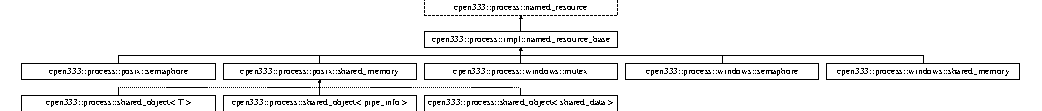
\includegraphics[height=1.493333cm]{classcpen333_1_1process_1_1impl_1_1named__resource__base}
\end{center}
\end{figure}
\subsection*{Public Member Functions}
\begin{DoxyCompactItemize}
\item 
\hyperlink{classcpen333_1_1process_1_1impl_1_1named__resource__base_a5f6f8b6daec88189a041de4c60ad4518}{named\+\_\+resource\+\_\+base} (const std\+::string \&\hyperlink{classcpen333_1_1process_1_1impl_1_1named__resource__base_ae0c5fbb1843afe863cece4b51c38f807}{name})
\begin{DoxyCompactList}\small\item\em Constructor for base named resource. \end{DoxyCompactList}\item 
\mbox{\Hypertarget{classcpen333_1_1process_1_1impl_1_1named__resource__base_ae53d159d6c0d58a37ce8091aa132e11b}\label{classcpen333_1_1process_1_1impl_1_1named__resource__base_ae53d159d6c0d58a37ce8091aa132e11b}} 
virtual \hyperlink{classcpen333_1_1process_1_1impl_1_1named__resource__base_ae53d159d6c0d58a37ce8091aa132e11b}{$\sim$named\+\_\+resource\+\_\+base} ()
\begin{DoxyCompactList}\small\item\em Destructor, does nothing. \end{DoxyCompactList}\item 
virtual bool \hyperlink{classcpen333_1_1process_1_1impl_1_1named__resource__base_ae4033f82dfd068b917a9bca57d3a0c45}{unlink} ()=0
\begin{DoxyCompactList}\small\item\em Detaches the name from the named resource. \end{DoxyCompactList}\end{DoxyCompactItemize}
\subsection*{Static Public Member Functions}
\begin{DoxyCompactItemize}
\item 
static bool \hyperlink{classcpen333_1_1process_1_1impl_1_1named__resource__base_a47a1396cf7c8210e76431a4ba4725146}{unlink} (const std\+::string \&\hyperlink{classcpen333_1_1process_1_1impl_1_1named__resource__base_ae0c5fbb1843afe863cece4b51c38f807}{name})
\begin{DoxyCompactList}\small\item\em Unlinks the name without needing to create a resource. \end{DoxyCompactList}\end{DoxyCompactItemize}
\subsection*{Protected Member Functions}
\begin{DoxyCompactItemize}
\item 
std\+::string \hyperlink{classcpen333_1_1process_1_1impl_1_1named__resource__base_ae0c5fbb1843afe863cece4b51c38f807}{name} () const
\begin{DoxyCompactList}\small\item\em Internal-\/use system name. \end{DoxyCompactList}\item 
const char $\ast$ \hyperlink{classcpen333_1_1process_1_1impl_1_1named__resource__base_af4f2889b26cf33d0d5ed794b7e4097ab}{name\+\_\+ptr} () const
\begin{DoxyCompactList}\small\item\em Internal-\/use system name as char pointer. \end{DoxyCompactList}\end{DoxyCompactItemize}
\subsection*{Static Protected Member Functions}
\begin{DoxyCompactItemize}
\item 
static void \hyperlink{classcpen333_1_1process_1_1impl_1_1named__resource__base_a3a513fc13851a3a72b4cc5ea8aa0e104}{make\+\_\+resource\+\_\+name} (const std\+::string \&\hyperlink{classcpen333_1_1process_1_1impl_1_1named__resource__base_ae0c5fbb1843afe863cece4b51c38f807}{name}, char out\mbox{[}$\,$\mbox{]})
\begin{DoxyCompactList}\small\item\em Creates a valid resource name. \end{DoxyCompactList}\end{DoxyCompactItemize}


\subsection{Detailed Description}
Base-\/class for named resources. 

Stores a unique identifier name 

\subsection{Constructor \& Destructor Documentation}
\mbox{\Hypertarget{classcpen333_1_1process_1_1impl_1_1named__resource__base_a5f6f8b6daec88189a041de4c60ad4518}\label{classcpen333_1_1process_1_1impl_1_1named__resource__base_a5f6f8b6daec88189a041de4c60ad4518}} 
\index{cpen333\+::process\+::impl\+::named\+\_\+resource\+\_\+base@{cpen333\+::process\+::impl\+::named\+\_\+resource\+\_\+base}!named\+\_\+resource\+\_\+base@{named\+\_\+resource\+\_\+base}}
\index{named\+\_\+resource\+\_\+base@{named\+\_\+resource\+\_\+base}!cpen333\+::process\+::impl\+::named\+\_\+resource\+\_\+base@{cpen333\+::process\+::impl\+::named\+\_\+resource\+\_\+base}}
\subsubsection{\texorpdfstring{named\+\_\+resource\+\_\+base()}{named\_resource\_base()}}
{\footnotesize\ttfamily cpen333\+::process\+::impl\+::named\+\_\+resource\+\_\+base\+::named\+\_\+resource\+\_\+base (\begin{DoxyParamCaption}\item[{const std\+::string \&}]{name }\end{DoxyParamCaption})\hspace{0.3cm}{\ttfamily [inline]}}



Constructor for base named resource. 


\begin{DoxyParams}{Parameters}
{\em name} & unique identifier \\
\hline
\end{DoxyParams}


\subsection{Member Function Documentation}
\mbox{\Hypertarget{classcpen333_1_1process_1_1impl_1_1named__resource__base_a3a513fc13851a3a72b4cc5ea8aa0e104}\label{classcpen333_1_1process_1_1impl_1_1named__resource__base_a3a513fc13851a3a72b4cc5ea8aa0e104}} 
\index{cpen333\+::process\+::impl\+::named\+\_\+resource\+\_\+base@{cpen333\+::process\+::impl\+::named\+\_\+resource\+\_\+base}!make\+\_\+resource\+\_\+name@{make\+\_\+resource\+\_\+name}}
\index{make\+\_\+resource\+\_\+name@{make\+\_\+resource\+\_\+name}!cpen333\+::process\+::impl\+::named\+\_\+resource\+\_\+base@{cpen333\+::process\+::impl\+::named\+\_\+resource\+\_\+base}}
\subsubsection{\texorpdfstring{make\+\_\+resource\+\_\+name()}{make\_resource\_name()}}
{\footnotesize\ttfamily static void cpen333\+::process\+::impl\+::named\+\_\+resource\+\_\+base\+::make\+\_\+resource\+\_\+name (\begin{DoxyParamCaption}\item[{const std\+::string \&}]{name,  }\item[{char}]{out\mbox{[}$\,$\mbox{]} }\end{DoxyParamCaption})\hspace{0.3cm}{\ttfamily [inline]}, {\ttfamily [static]}, {\ttfamily [protected]}}



Creates a valid resource name. 

Creates a valid resource name for the platform, on Linux/\+O\+SX this is a leading \textquotesingle{}/\textquotesingle{} with sha1 base64-\/encoded hash of the string name. We will also replace any other \textquotesingle{}/\textquotesingle{} with \textquotesingle{}\+\_\+\textquotesingle{} 
\begin{DoxyParams}{Parameters}
{\em name} & original resource name \\
\hline
{\em out} & platform-\/safe resource name \\
\hline
\end{DoxyParams}
\mbox{\Hypertarget{classcpen333_1_1process_1_1impl_1_1named__resource__base_ae0c5fbb1843afe863cece4b51c38f807}\label{classcpen333_1_1process_1_1impl_1_1named__resource__base_ae0c5fbb1843afe863cece4b51c38f807}} 
\index{cpen333\+::process\+::impl\+::named\+\_\+resource\+\_\+base@{cpen333\+::process\+::impl\+::named\+\_\+resource\+\_\+base}!name@{name}}
\index{name@{name}!cpen333\+::process\+::impl\+::named\+\_\+resource\+\_\+base@{cpen333\+::process\+::impl\+::named\+\_\+resource\+\_\+base}}
\subsubsection{\texorpdfstring{name()}{name()}}
{\footnotesize\ttfamily std\+::string cpen333\+::process\+::impl\+::named\+\_\+resource\+\_\+base\+::name (\begin{DoxyParamCaption}{ }\end{DoxyParamCaption}) const\hspace{0.3cm}{\ttfamily [inline]}, {\ttfamily [protected]}}



Internal-\/use system name. 

\begin{DoxyReturn}{Returns}
underlying unique identifier name 
\end{DoxyReturn}
\mbox{\Hypertarget{classcpen333_1_1process_1_1impl_1_1named__resource__base_af4f2889b26cf33d0d5ed794b7e4097ab}\label{classcpen333_1_1process_1_1impl_1_1named__resource__base_af4f2889b26cf33d0d5ed794b7e4097ab}} 
\index{cpen333\+::process\+::impl\+::named\+\_\+resource\+\_\+base@{cpen333\+::process\+::impl\+::named\+\_\+resource\+\_\+base}!name\+\_\+ptr@{name\+\_\+ptr}}
\index{name\+\_\+ptr@{name\+\_\+ptr}!cpen333\+::process\+::impl\+::named\+\_\+resource\+\_\+base@{cpen333\+::process\+::impl\+::named\+\_\+resource\+\_\+base}}
\subsubsection{\texorpdfstring{name\+\_\+ptr()}{name\_ptr()}}
{\footnotesize\ttfamily const char$\ast$ cpen333\+::process\+::impl\+::named\+\_\+resource\+\_\+base\+::name\+\_\+ptr (\begin{DoxyParamCaption}{ }\end{DoxyParamCaption}) const\hspace{0.3cm}{\ttfamily [inline]}, {\ttfamily [protected]}}



Internal-\/use system name as char pointer. 

\begin{DoxyReturn}{Returns}
pointer to underlying unique identifier name 
\end{DoxyReturn}
\mbox{\Hypertarget{classcpen333_1_1process_1_1impl_1_1named__resource__base_ae4033f82dfd068b917a9bca57d3a0c45}\label{classcpen333_1_1process_1_1impl_1_1named__resource__base_ae4033f82dfd068b917a9bca57d3a0c45}} 
\index{cpen333\+::process\+::impl\+::named\+\_\+resource\+\_\+base@{cpen333\+::process\+::impl\+::named\+\_\+resource\+\_\+base}!unlink@{unlink}}
\index{unlink@{unlink}!cpen333\+::process\+::impl\+::named\+\_\+resource\+\_\+base@{cpen333\+::process\+::impl\+::named\+\_\+resource\+\_\+base}}
\subsubsection{\texorpdfstring{unlink()}{unlink()}\hspace{0.1cm}{\footnotesize\ttfamily [1/2]}}
{\footnotesize\ttfamily virtual bool cpen333\+::process\+::impl\+::named\+\_\+resource\+\_\+base\+::unlink (\begin{DoxyParamCaption}{ }\end{DoxyParamCaption})\hspace{0.3cm}{\ttfamily [pure virtual]}}



Detaches the name from the named resource. 

On P\+O\+S\+IX systems, named resources will persist beyond the lifetime of any process that uses them as long as the name has not been unlinked (or until the system is rebooted). Calling {\ttfamily unlink} will detach the name, allowing the resource to be freed once all current users have exited.

\begin{DoxyReturn}{Returns}
{\ttfamily true} if unlink is successful, {\ttfamily false} if unlinking is not supported or if an error has occurred. 
\end{DoxyReturn}


Implements \hyperlink{classcpen333_1_1process_1_1named__resource_a5d33168fee48c9b0c58ab8fd96e230ce}{cpen333\+::process\+::named\+\_\+resource}.



Implemented in \hyperlink{classcpen333_1_1process_1_1posix_1_1semaphore_aa6064e2c4b4b7282cc5e6eda877ee1bb}{cpen333\+::process\+::posix\+::semaphore}, \hyperlink{classcpen333_1_1process_1_1windows_1_1semaphore_abc5159f32e61024c6c6a978ac64fe39d}{cpen333\+::process\+::windows\+::semaphore}, \hyperlink{classcpen333_1_1process_1_1windows_1_1shared__memory_aa6efdc9a3e1310ea69ecc48aeb41286c}{cpen333\+::process\+::windows\+::shared\+\_\+memory}, \hyperlink{classcpen333_1_1process_1_1windows_1_1mutex_aa45381a0a226fbefc86eef8971a5431b}{cpen333\+::process\+::windows\+::mutex}, \hyperlink{classcpen333_1_1process_1_1posix_1_1shared__memory_a3b6d67a41cfaca3712d87958682d8bbe}{cpen333\+::process\+::posix\+::shared\+\_\+memory}, \hyperlink{classcpen333_1_1process_1_1shared__object_aa5b43829da5bd2376927e6285745211c}{cpen333\+::process\+::shared\+\_\+object$<$ T $>$}, \hyperlink{classcpen333_1_1process_1_1shared__object_aa5b43829da5bd2376927e6285745211c}{cpen333\+::process\+::shared\+\_\+object$<$ pipe\+\_\+info $>$}, and \hyperlink{classcpen333_1_1process_1_1shared__object_aa5b43829da5bd2376927e6285745211c}{cpen333\+::process\+::shared\+\_\+object$<$ shared\+\_\+data $>$}.

\mbox{\Hypertarget{classcpen333_1_1process_1_1impl_1_1named__resource__base_a47a1396cf7c8210e76431a4ba4725146}\label{classcpen333_1_1process_1_1impl_1_1named__resource__base_a47a1396cf7c8210e76431a4ba4725146}} 
\index{cpen333\+::process\+::impl\+::named\+\_\+resource\+\_\+base@{cpen333\+::process\+::impl\+::named\+\_\+resource\+\_\+base}!unlink@{unlink}}
\index{unlink@{unlink}!cpen333\+::process\+::impl\+::named\+\_\+resource\+\_\+base@{cpen333\+::process\+::impl\+::named\+\_\+resource\+\_\+base}}
\subsubsection{\texorpdfstring{unlink()}{unlink()}\hspace{0.1cm}{\footnotesize\ttfamily [2/2]}}
{\footnotesize\ttfamily static bool cpen333\+::process\+::impl\+::named\+\_\+resource\+\_\+base\+::unlink (\begin{DoxyParamCaption}\item[{const std\+::string \&}]{name }\end{DoxyParamCaption})\hspace{0.3cm}{\ttfamily [inline]}, {\ttfamily [static]}}



Unlinks the name without needing to create a resource. 

Implementers should also provide a static method for unlinking. The purpose is mainly for clean-\/up of existing resources.


\begin{DoxyParams}{Parameters}
{\em name} & desired resource name \\
\hline
\end{DoxyParams}
\begin{DoxyReturn}{Returns}
{\ttfamily true} if unlink successful, {\ttfamily false} if not successful or not supported 
\end{DoxyReturn}


The documentation for this class was generated from the following file\+:\begin{DoxyCompactItemize}
\item 
D\+:/school/teaching/\+C\+P\+E\+N333/workspace/library/include/cpen333/process/impl/\hyperlink{named__resource__base_8h}{named\+\_\+resource\+\_\+base.\+h}\end{DoxyCompactItemize}

\hypertarget{classcpen333_1_1process_1_1pipe}{}\section{cpen333\+:\+:process\+:\+:pipe Class Reference}
\label{classcpen333_1_1process_1_1pipe}\index{cpen333\+::process\+::pipe@{cpen333\+::process\+::pipe}}


Inter-\/process pipe with one read-\/end and one write-\/end, emulated using a shared F\+I\+F\+O-\/style queue.  




{\ttfamily \#include $<$pipe.\+h$>$}

Inheritance diagram for cpen333\+:\+:process\+:\+:pipe\+:\begin{figure}[H]
\begin{center}
\leavevmode
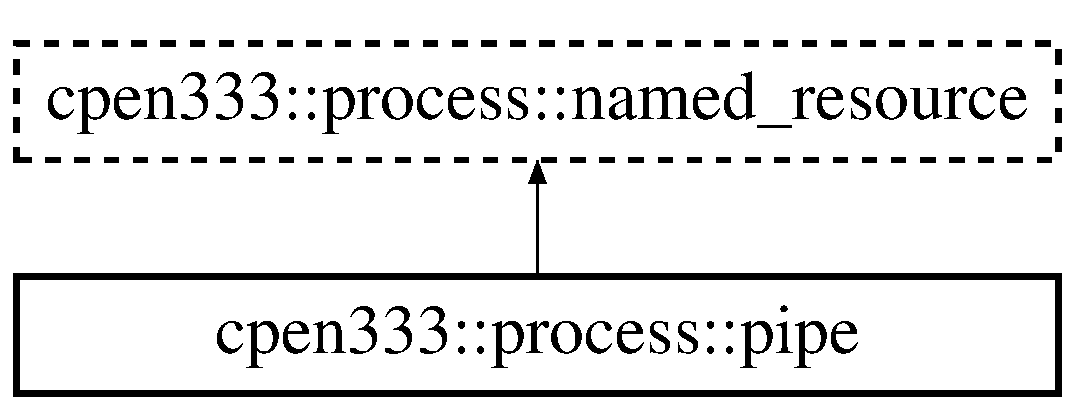
\includegraphics[height=2.000000cm]{classcpen333_1_1process_1_1pipe}
\end{center}
\end{figure}
\subsection*{Public Types}
\begin{DoxyCompactItemize}
\item 
enum \hyperlink{classcpen333_1_1process_1_1pipe_a80047f44ba5638538b032efa851c6f3c}{mode} \{ \hyperlink{classcpen333_1_1process_1_1pipe_a80047f44ba5638538b032efa851c6f3ca683aa54088bc99c7fe5143db2db483fb}{R\+E\+AD}, 
\hyperlink{classcpen333_1_1process_1_1pipe_a80047f44ba5638538b032efa851c6f3caf7d3bc474155ae5295e3b8f0873e83fe}{W\+R\+I\+TE}
 \}\begin{DoxyCompactList}\small\item\em pipe access mode \end{DoxyCompactList}
\end{DoxyCompactItemize}
\subsection*{Public Member Functions}
\begin{DoxyCompactItemize}
\item 
\hyperlink{classcpen333_1_1process_1_1pipe_a87d45160992c6f27c7291ef3a0f118bf}{pipe} (const std\+::string \&name, \hyperlink{classcpen333_1_1process_1_1pipe_a80047f44ba5638538b032efa851c6f3c}{mode} \hyperlink{classcpen333_1_1process_1_1pipe_a80047f44ba5638538b032efa851c6f3c}{mode}, size\+\_\+t size=1024)
\begin{DoxyCompactList}\small\item\em Constructs a named pipe instance. \end{DoxyCompactList}\item 
\mbox{\Hypertarget{classcpen333_1_1process_1_1pipe_a913c91ae5dce8df7fd836b43d541598f}\label{classcpen333_1_1process_1_1pipe_a913c91ae5dce8df7fd836b43d541598f}} 
virtual \hyperlink{classcpen333_1_1process_1_1pipe_a913c91ae5dce8df7fd836b43d541598f}{$\sim$pipe} ()
\begin{DoxyCompactList}\small\item\em Destructor, automatically closes the pipe. \end{DoxyCompactList}\item 
bool \hyperlink{classcpen333_1_1process_1_1pipe_afa2e2598bf72fa411b4b96bbf88d2f4b}{write} (const void $\ast$data, size\+\_\+t size)
\begin{DoxyCompactList}\small\item\em Writes data to the pipe. \end{DoxyCompactList}\item 
{\footnotesize template$<$typename T $>$ }\\bool \hyperlink{classcpen333_1_1process_1_1pipe_aa13d4d9154d30a7d3df953006a4e3019}{write} (const T \&data)
\begin{DoxyCompactList}\small\item\em Writes an object to the pipe. \end{DoxyCompactList}\item 
{\footnotesize template$<$typename T $>$ }\\bool \hyperlink{classcpen333_1_1process_1_1pipe_ab6f8f7992592df4cf0d24307881cd58d}{write} (const T $\ast$data)
\begin{DoxyCompactList}\small\item\em Writes an object to the pipe. \end{DoxyCompactList}\item 
bool \hyperlink{classcpen333_1_1process_1_1pipe_ae25219bad758b0b54887addb2d6bd729}{read} (void $\ast$data, size\+\_\+t size)
\begin{DoxyCompactList}\small\item\em Reads data from the pipe. \end{DoxyCompactList}\item 
uint8\+\_\+t \hyperlink{classcpen333_1_1process_1_1pipe_a165e12b1cb0fc16f1732e29b8022d7df}{read} ()
\begin{DoxyCompactList}\small\item\em Read a single byte. \end{DoxyCompactList}\item 
{\footnotesize template$<$typename T $>$ }\\bool \hyperlink{classcpen333_1_1process_1_1pipe_a67c555d0003807fcbc8a3ae1b6ee0f97}{read} (T $\ast$data)
\begin{DoxyCompactList}\small\item\em Reads an object from the pipe. \end{DoxyCompactList}\item 
size\+\_\+t \hyperlink{classcpen333_1_1process_1_1pipe_a5d5e3145f376e1b77e3ebe0580e99fd1}{available} ()
\begin{DoxyCompactList}\small\item\em Determines the number of bytes currently remaining in the pipe. \end{DoxyCompactList}\item 
void \hyperlink{classcpen333_1_1process_1_1pipe_abe03b5f5eacd1546db7a0ef6ffb3ba71}{close} ()
\begin{DoxyCompactList}\small\item\em closes one end of the pipe \end{DoxyCompactList}\item 
bool \hyperlink{classcpen333_1_1process_1_1pipe_addcc650694ad0712637874eb79ec8407}{unlink} ()
\begin{DoxyCompactList}\small\item\em Detaches the name from the named resource. \end{DoxyCompactList}\end{DoxyCompactItemize}
\subsection*{Static Public Member Functions}
\begin{DoxyCompactItemize}
\item 
static bool \hyperlink{classcpen333_1_1process_1_1pipe_ad0d66f9fc3712849b6af36ca7d19e54d}{unlink} (const std\+::string \&name)
\begin{DoxyCompactList}\small\item\em Unlinks the name without needing to create a resource. \end{DoxyCompactList}\end{DoxyCompactItemize}


\subsection{Detailed Description}
Inter-\/process pipe with one read-\/end and one write-\/end, emulated using a shared F\+I\+F\+O-\/style queue. 

Allows sending/receiving of unstructured information between two connected processes. One process must be designated as the reader and the other as the writer. 

\subsection{Member Enumeration Documentation}
\mbox{\Hypertarget{classcpen333_1_1process_1_1pipe_a80047f44ba5638538b032efa851c6f3c}\label{classcpen333_1_1process_1_1pipe_a80047f44ba5638538b032efa851c6f3c}} 
\index{cpen333\+::process\+::pipe@{cpen333\+::process\+::pipe}!mode@{mode}}
\index{mode@{mode}!cpen333\+::process\+::pipe@{cpen333\+::process\+::pipe}}
\subsubsection{\texorpdfstring{mode}{mode}}
{\footnotesize\ttfamily enum \hyperlink{classcpen333_1_1process_1_1pipe_a80047f44ba5638538b032efa851c6f3c}{cpen333\+::process\+::pipe\+::mode}}



pipe access mode 

\begin{DoxyEnumFields}{Enumerator}
\raisebox{\heightof{T}}[0pt][0pt]{\index{R\+E\+AD@{R\+E\+AD}!cpen333\+::process\+::pipe@{cpen333\+::process\+::pipe}}\index{cpen333\+::process\+::pipe@{cpen333\+::process\+::pipe}!R\+E\+AD@{R\+E\+AD}}}\mbox{\Hypertarget{classcpen333_1_1process_1_1pipe_a80047f44ba5638538b032efa851c6f3ca683aa54088bc99c7fe5143db2db483fb}\label{classcpen333_1_1process_1_1pipe_a80047f44ba5638538b032efa851c6f3ca683aa54088bc99c7fe5143db2db483fb}} 
R\+E\+AD&open read-\/end of pipe \\
\hline

\raisebox{\heightof{T}}[0pt][0pt]{\index{W\+R\+I\+TE@{W\+R\+I\+TE}!cpen333\+::process\+::pipe@{cpen333\+::process\+::pipe}}\index{cpen333\+::process\+::pipe@{cpen333\+::process\+::pipe}!W\+R\+I\+TE@{W\+R\+I\+TE}}}\mbox{\Hypertarget{classcpen333_1_1process_1_1pipe_a80047f44ba5638538b032efa851c6f3caf7d3bc474155ae5295e3b8f0873e83fe}\label{classcpen333_1_1process_1_1pipe_a80047f44ba5638538b032efa851c6f3caf7d3bc474155ae5295e3b8f0873e83fe}} 
W\+R\+I\+TE&open write-\/end of pipe \\
\hline

\end{DoxyEnumFields}


\subsection{Constructor \& Destructor Documentation}
\mbox{\Hypertarget{classcpen333_1_1process_1_1pipe_a87d45160992c6f27c7291ef3a0f118bf}\label{classcpen333_1_1process_1_1pipe_a87d45160992c6f27c7291ef3a0f118bf}} 
\index{cpen333\+::process\+::pipe@{cpen333\+::process\+::pipe}!pipe@{pipe}}
\index{pipe@{pipe}!cpen333\+::process\+::pipe@{cpen333\+::process\+::pipe}}
\subsubsection{\texorpdfstring{pipe()}{pipe()}}
{\footnotesize\ttfamily cpen333\+::process\+::pipe\+::pipe (\begin{DoxyParamCaption}\item[{const std\+::string \&}]{name,  }\item[{\hyperlink{classcpen333_1_1process_1_1pipe_a80047f44ba5638538b032efa851c6f3c}{mode}}]{mode,  }\item[{size\+\_\+t}]{size = {\ttfamily 1024} }\end{DoxyParamCaption})\hspace{0.3cm}{\ttfamily [inline]}}



Constructs a named pipe instance. 


\begin{DoxyParams}{Parameters}
{\em name} & identifier for creating or connecting to an existing inter-\/process pip \\
\hline
{\em mode} & access mode, either read or write \\
\hline
{\em size} & if creating, the maximum number of bytes that can be stored in the pipe without blocking \\
\hline
\end{DoxyParams}


\subsection{Member Function Documentation}
\mbox{\Hypertarget{classcpen333_1_1process_1_1pipe_a5d5e3145f376e1b77e3ebe0580e99fd1}\label{classcpen333_1_1process_1_1pipe_a5d5e3145f376e1b77e3ebe0580e99fd1}} 
\index{cpen333\+::process\+::pipe@{cpen333\+::process\+::pipe}!available@{available}}
\index{available@{available}!cpen333\+::process\+::pipe@{cpen333\+::process\+::pipe}}
\subsubsection{\texorpdfstring{available()}{available()}}
{\footnotesize\ttfamily size\+\_\+t cpen333\+::process\+::pipe\+::available (\begin{DoxyParamCaption}{ }\end{DoxyParamCaption})\hspace{0.3cm}{\ttfamily [inline]}}



Determines the number of bytes currently remaining in the pipe. 

This method should rarely be used, as the number of bytes is subject to change rapidly. One possible use-\/case is if there is a single reader, and the reader wants to check if there is any data available.

\begin{DoxyReturn}{Returns}
number of bytes currently remaining in the pipe 
\end{DoxyReturn}
\mbox{\Hypertarget{classcpen333_1_1process_1_1pipe_abe03b5f5eacd1546db7a0ef6ffb3ba71}\label{classcpen333_1_1process_1_1pipe_abe03b5f5eacd1546db7a0ef6ffb3ba71}} 
\index{cpen333\+::process\+::pipe@{cpen333\+::process\+::pipe}!close@{close}}
\index{close@{close}!cpen333\+::process\+::pipe@{cpen333\+::process\+::pipe}}
\subsubsection{\texorpdfstring{close()}{close()}}
{\footnotesize\ttfamily void cpen333\+::process\+::pipe\+::close (\begin{DoxyParamCaption}{ }\end{DoxyParamCaption})\hspace{0.3cm}{\ttfamily [inline]}}



closes one end of the pipe 

If the current instance is a reader, then closes the read-\/end of the pipe. If a writer, closes, the write-\/end. \mbox{\Hypertarget{classcpen333_1_1process_1_1pipe_ae25219bad758b0b54887addb2d6bd729}\label{classcpen333_1_1process_1_1pipe_ae25219bad758b0b54887addb2d6bd729}} 
\index{cpen333\+::process\+::pipe@{cpen333\+::process\+::pipe}!read@{read}}
\index{read@{read}!cpen333\+::process\+::pipe@{cpen333\+::process\+::pipe}}
\subsubsection{\texorpdfstring{read()}{read()}\hspace{0.1cm}{\footnotesize\ttfamily [1/3]}}
{\footnotesize\ttfamily bool cpen333\+::process\+::pipe\+::read (\begin{DoxyParamCaption}\item[{void $\ast$}]{data,  }\item[{size\+\_\+t}]{size }\end{DoxyParamCaption})\hspace{0.3cm}{\ttfamily [inline]}}



Reads data from the pipe. 

Reads the specified number of bytes from the head of the pipe. This method will block until the desired number of bytes are read.


\begin{DoxyParams}{Parameters}
{\em data} & memory address to fill with pipe contents \\
\hline
{\em size} & number of bytes \\
\hline
\end{DoxyParams}
\begin{DoxyReturn}{Returns}
true if successful, false if not opened in read mode, or pipe is closed and does not have enough bytes left 
\end{DoxyReturn}
\mbox{\Hypertarget{classcpen333_1_1process_1_1pipe_a165e12b1cb0fc16f1732e29b8022d7df}\label{classcpen333_1_1process_1_1pipe_a165e12b1cb0fc16f1732e29b8022d7df}} 
\index{cpen333\+::process\+::pipe@{cpen333\+::process\+::pipe}!read@{read}}
\index{read@{read}!cpen333\+::process\+::pipe@{cpen333\+::process\+::pipe}}
\subsubsection{\texorpdfstring{read()}{read()}\hspace{0.1cm}{\footnotesize\ttfamily [2/3]}}
{\footnotesize\ttfamily uint8\+\_\+t cpen333\+::process\+::pipe\+::read (\begin{DoxyParamCaption}{ }\end{DoxyParamCaption})\hspace{0.3cm}{\ttfamily [inline]}}



Read a single byte. 

\begin{DoxyReturn}{Returns}
next byte in the stream 
\end{DoxyReturn}
\mbox{\Hypertarget{classcpen333_1_1process_1_1pipe_a67c555d0003807fcbc8a3ae1b6ee0f97}\label{classcpen333_1_1process_1_1pipe_a67c555d0003807fcbc8a3ae1b6ee0f97}} 
\index{cpen333\+::process\+::pipe@{cpen333\+::process\+::pipe}!read@{read}}
\index{read@{read}!cpen333\+::process\+::pipe@{cpen333\+::process\+::pipe}}
\subsubsection{\texorpdfstring{read()}{read()}\hspace{0.1cm}{\footnotesize\ttfamily [3/3]}}
{\footnotesize\ttfamily template$<$typename T $>$ \\
bool cpen333\+::process\+::pipe\+::read (\begin{DoxyParamCaption}\item[{T $\ast$}]{data }\end{DoxyParamCaption})\hspace{0.3cm}{\ttfamily [inline]}}



Reads an object from the pipe. 

Convenience method for reading an object from the pipe, auto-\/detecting the appropriate number of bytes to read. This method will block until the complete object is read.


\begin{DoxyTemplParams}{Template Parameters}
{\em T} & type of object \\
\hline
\end{DoxyTemplParams}

\begin{DoxyParams}{Parameters}
{\em data} & pointer to object to populate \\
\hline
\end{DoxyParams}
\begin{DoxyReturn}{Returns}
true if successful, false if not opened in read mode, or pipe is closed and does not have enough bytes left 
\end{DoxyReturn}
\mbox{\Hypertarget{classcpen333_1_1process_1_1pipe_addcc650694ad0712637874eb79ec8407}\label{classcpen333_1_1process_1_1pipe_addcc650694ad0712637874eb79ec8407}} 
\index{cpen333\+::process\+::pipe@{cpen333\+::process\+::pipe}!unlink@{unlink}}
\index{unlink@{unlink}!cpen333\+::process\+::pipe@{cpen333\+::process\+::pipe}}
\subsubsection{\texorpdfstring{unlink()}{unlink()}\hspace{0.1cm}{\footnotesize\ttfamily [1/2]}}
{\footnotesize\ttfamily bool cpen333\+::process\+::pipe\+::unlink (\begin{DoxyParamCaption}{ }\end{DoxyParamCaption})\hspace{0.3cm}{\ttfamily [inline]}, {\ttfamily [virtual]}}



Detaches the name from the named resource. 

On P\+O\+S\+IX systems, named resources will persist beyond the lifetime of any process that uses them as long as the name has not been unlinked (or until the system is rebooted). Calling {\ttfamily unlink} will detach the name, allowing the resource to be freed once all current users have exited.

\begin{DoxyReturn}{Returns}
{\ttfamily true} if unlink is successful, {\ttfamily false} if unlinking is not supported or if an error has occurred. 
\end{DoxyReturn}


Implements \hyperlink{classcpen333_1_1process_1_1named__resource_a5d33168fee48c9b0c58ab8fd96e230ce}{cpen333\+::process\+::named\+\_\+resource}.

\mbox{\Hypertarget{classcpen333_1_1process_1_1pipe_ad0d66f9fc3712849b6af36ca7d19e54d}\label{classcpen333_1_1process_1_1pipe_ad0d66f9fc3712849b6af36ca7d19e54d}} 
\index{cpen333\+::process\+::pipe@{cpen333\+::process\+::pipe}!unlink@{unlink}}
\index{unlink@{unlink}!cpen333\+::process\+::pipe@{cpen333\+::process\+::pipe}}
\subsubsection{\texorpdfstring{unlink()}{unlink()}\hspace{0.1cm}{\footnotesize\ttfamily [2/2]}}
{\footnotesize\ttfamily static bool cpen333\+::process\+::pipe\+::unlink (\begin{DoxyParamCaption}\item[{const std\+::string \&}]{name }\end{DoxyParamCaption})\hspace{0.3cm}{\ttfamily [inline]}, {\ttfamily [static]}}



Unlinks the name without needing to create a resource. 

Implementers should also provide a static method for unlinking. The purpose is mainly for clean-\/up of existing resources.


\begin{DoxyParams}{Parameters}
{\em name} & desired resource name \\
\hline
\end{DoxyParams}
\begin{DoxyReturn}{Returns}
{\ttfamily true} if unlink successful, {\ttfamily false} if not successful or not supported 
\end{DoxyReturn}
\mbox{\Hypertarget{classcpen333_1_1process_1_1pipe_afa2e2598bf72fa411b4b96bbf88d2f4b}\label{classcpen333_1_1process_1_1pipe_afa2e2598bf72fa411b4b96bbf88d2f4b}} 
\index{cpen333\+::process\+::pipe@{cpen333\+::process\+::pipe}!write@{write}}
\index{write@{write}!cpen333\+::process\+::pipe@{cpen333\+::process\+::pipe}}
\subsubsection{\texorpdfstring{write()}{write()}\hspace{0.1cm}{\footnotesize\ttfamily [1/3]}}
{\footnotesize\ttfamily bool cpen333\+::process\+::pipe\+::write (\begin{DoxyParamCaption}\item[{const void $\ast$}]{data,  }\item[{size\+\_\+t}]{size }\end{DoxyParamCaption})\hspace{0.3cm}{\ttfamily [inline]}}



Writes data to the pipe. 

If the pipe becomes full, will block until there is room to complete the message.


\begin{DoxyParams}{Parameters}
{\em data} & data to write \\
\hline
{\em size} & number of bytes to write \\
\hline
\end{DoxyParams}
\begin{DoxyReturn}{Returns}
true if pipe is open and write is successful, false if pipe is closed or we are not in W\+R\+I\+TE mode 
\end{DoxyReturn}
\mbox{\Hypertarget{classcpen333_1_1process_1_1pipe_aa13d4d9154d30a7d3df953006a4e3019}\label{classcpen333_1_1process_1_1pipe_aa13d4d9154d30a7d3df953006a4e3019}} 
\index{cpen333\+::process\+::pipe@{cpen333\+::process\+::pipe}!write@{write}}
\index{write@{write}!cpen333\+::process\+::pipe@{cpen333\+::process\+::pipe}}
\subsubsection{\texorpdfstring{write()}{write()}\hspace{0.1cm}{\footnotesize\ttfamily [2/3]}}
{\footnotesize\ttfamily template$<$typename T $>$ \\
bool cpen333\+::process\+::pipe\+::write (\begin{DoxyParamCaption}\item[{const T \&}]{data }\end{DoxyParamCaption})\hspace{0.3cm}{\ttfamily [inline]}}



Writes an object to the pipe. 

Convenience method for writing objects to the pipe, auto-\/detecting the appropriate number of bytes. This method will block until there is sufficient room to finish writing the object


\begin{DoxyTemplParams}{Template Parameters}
{\em T} & type of object to write \\
\hline
\end{DoxyTemplParams}

\begin{DoxyParams}{Parameters}
{\em data} & reference to data \\
\hline
\end{DoxyParams}
\begin{DoxyReturn}{Returns}
true if pipe is open and write is successful, false if pipe is closed or we are not in W\+R\+I\+TE mode 
\end{DoxyReturn}
\mbox{\Hypertarget{classcpen333_1_1process_1_1pipe_ab6f8f7992592df4cf0d24307881cd58d}\label{classcpen333_1_1process_1_1pipe_ab6f8f7992592df4cf0d24307881cd58d}} 
\index{cpen333\+::process\+::pipe@{cpen333\+::process\+::pipe}!write@{write}}
\index{write@{write}!cpen333\+::process\+::pipe@{cpen333\+::process\+::pipe}}
\subsubsection{\texorpdfstring{write()}{write()}\hspace{0.1cm}{\footnotesize\ttfamily [3/3]}}
{\footnotesize\ttfamily template$<$typename T $>$ \\
bool cpen333\+::process\+::pipe\+::write (\begin{DoxyParamCaption}\item[{const T $\ast$}]{data }\end{DoxyParamCaption})\hspace{0.3cm}{\ttfamily [inline]}}



Writes an object to the pipe. 

Convenience method for writing objects to the pipe, auto-\/detecting the appropriate number of bytes. This method will block until there is sufficient room to finish writing the object


\begin{DoxyTemplParams}{Template Parameters}
{\em T} & type of object to write \\
\hline
\end{DoxyTemplParams}

\begin{DoxyParams}{Parameters}
{\em data} & pointer to data \\
\hline
\end{DoxyParams}
\begin{DoxyReturn}{Returns}
true if pipe is open and write is successful, false if pipe is closed or we are not in W\+R\+I\+TE mode 
\end{DoxyReturn}


The documentation for this class was generated from the following file\+:\begin{DoxyCompactItemize}
\item 
D\+:/school/teaching/\+C\+P\+E\+N333/workspace/labs/include/cpen333/process/\hyperlink{pipe_8h}{pipe.\+h}\end{DoxyCompactItemize}

\hypertarget{classcpen333_1_1process_1_1rendezvous}{}\section{cpen333\+:\+:process\+:\+:rendezvous Class Reference}
\label{classcpen333_1_1process_1_1rendezvous}\index{cpen333\+::process\+::rendezvous@{cpen333\+::process\+::rendezvous}}


Inter-\/process rendezvous implementation.  




{\ttfamily \#include $<$rendezvous.\+h$>$}

Inheritance diagram for cpen333\+:\+:process\+:\+:rendezvous\+:\begin{figure}[H]
\begin{center}
\leavevmode
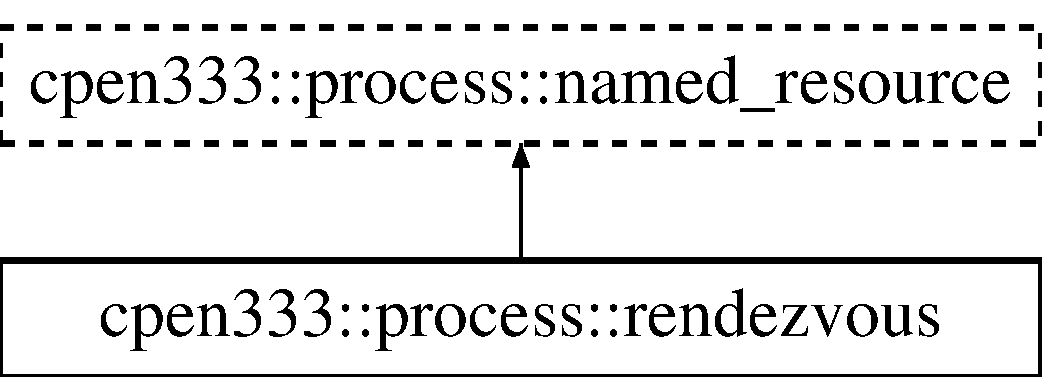
\includegraphics[height=2.000000cm]{classcpen333_1_1process_1_1rendezvous}
\end{center}
\end{figure}
\subsection*{Public Member Functions}
\begin{DoxyCompactItemize}
\item 
\hyperlink{classcpen333_1_1process_1_1rendezvous_a616069d02e03b2b33c7e10e730f084a0}{rendezvous} (const std\+::string \&name, size\+\_\+t size)
\begin{DoxyCompactList}\small\item\em Creates or connects to a named rendezvous primitive. \end{DoxyCompactList}\item 
void \hyperlink{classcpen333_1_1process_1_1rendezvous_a47603f8bc2aaf9302cb8132262912863}{wait} ()
\begin{DoxyCompactList}\small\item\em Waits until all other processes are also waiting. \end{DoxyCompactList}\item 
bool \hyperlink{classcpen333_1_1process_1_1rendezvous_a458242e8ba600b0e638421825cbc9589}{unlink} ()
\begin{DoxyCompactList}\small\item\em Detaches the name from the named resource. \end{DoxyCompactList}\end{DoxyCompactItemize}
\subsection*{Static Public Member Functions}
\begin{DoxyCompactItemize}
\item 
static bool \hyperlink{classcpen333_1_1process_1_1rendezvous_afc91e654e867c785656182d1b4adc360}{unlink} (const std\+::string \&name)
\begin{DoxyCompactList}\small\item\em Unlinks the name without needing to create a resource. \end{DoxyCompactList}\end{DoxyCompactItemize}


\subsection{Detailed Description}
Inter-\/process rendezvous implementation. 

A synchronization primitive that allows a certain number of threads/processes to wait for others to arrive, then proceed together. 

\subsection{Constructor \& Destructor Documentation}
\mbox{\Hypertarget{classcpen333_1_1process_1_1rendezvous_a616069d02e03b2b33c7e10e730f084a0}\label{classcpen333_1_1process_1_1rendezvous_a616069d02e03b2b33c7e10e730f084a0}} 
\index{cpen333\+::process\+::rendezvous@{cpen333\+::process\+::rendezvous}!rendezvous@{rendezvous}}
\index{rendezvous@{rendezvous}!cpen333\+::process\+::rendezvous@{cpen333\+::process\+::rendezvous}}
\subsubsection{\texorpdfstring{rendezvous()}{rendezvous()}}
{\footnotesize\ttfamily cpen333\+::process\+::rendezvous\+::rendezvous (\begin{DoxyParamCaption}\item[{const std\+::string \&}]{name,  }\item[{size\+\_\+t}]{size }\end{DoxyParamCaption})\hspace{0.3cm}{\ttfamily [inline]}}



Creates or connects to a named rendezvous primitive. 


\begin{DoxyParams}{Parameters}
{\em name} & identifier for creating or connecting to an existing inter-\/process rendezvous \\
\hline
{\em size} & number of processes in group \\
\hline
\end{DoxyParams}


\subsection{Member Function Documentation}
\mbox{\Hypertarget{classcpen333_1_1process_1_1rendezvous_a458242e8ba600b0e638421825cbc9589}\label{classcpen333_1_1process_1_1rendezvous_a458242e8ba600b0e638421825cbc9589}} 
\index{cpen333\+::process\+::rendezvous@{cpen333\+::process\+::rendezvous}!unlink@{unlink}}
\index{unlink@{unlink}!cpen333\+::process\+::rendezvous@{cpen333\+::process\+::rendezvous}}
\subsubsection{\texorpdfstring{unlink()}{unlink()}\hspace{0.1cm}{\footnotesize\ttfamily [1/2]}}
{\footnotesize\ttfamily bool cpen333\+::process\+::rendezvous\+::unlink (\begin{DoxyParamCaption}{ }\end{DoxyParamCaption})\hspace{0.3cm}{\ttfamily [inline]}, {\ttfamily [virtual]}}



Detaches the name from the named resource. 

On P\+O\+S\+IX systems, named resources will persist beyond the lifetime of any process that uses them as long as the name has not been unlinked (or until the system is rebooted). Calling {\ttfamily unlink} will detach the name, allowing the resource to be freed once all current users have exited.

\begin{DoxyReturn}{Returns}
{\ttfamily true} if unlink is successful, {\ttfamily false} if unlinking is not supported or if an error has occurred. 
\end{DoxyReturn}


Implements \hyperlink{classcpen333_1_1process_1_1named__resource_a5d33168fee48c9b0c58ab8fd96e230ce}{cpen333\+::process\+::named\+\_\+resource}.

\mbox{\Hypertarget{classcpen333_1_1process_1_1rendezvous_afc91e654e867c785656182d1b4adc360}\label{classcpen333_1_1process_1_1rendezvous_afc91e654e867c785656182d1b4adc360}} 
\index{cpen333\+::process\+::rendezvous@{cpen333\+::process\+::rendezvous}!unlink@{unlink}}
\index{unlink@{unlink}!cpen333\+::process\+::rendezvous@{cpen333\+::process\+::rendezvous}}
\subsubsection{\texorpdfstring{unlink()}{unlink()}\hspace{0.1cm}{\footnotesize\ttfamily [2/2]}}
{\footnotesize\ttfamily static bool cpen333\+::process\+::rendezvous\+::unlink (\begin{DoxyParamCaption}\item[{const std\+::string \&}]{name }\end{DoxyParamCaption})\hspace{0.3cm}{\ttfamily [inline]}, {\ttfamily [static]}}



Unlinks the name without needing to create a resource. 

Implementers should also provide a static method for unlinking. The purpose is mainly for clean-\/up of existing resources.


\begin{DoxyParams}{Parameters}
{\em name} & desired resource name \\
\hline
\end{DoxyParams}
\begin{DoxyReturn}{Returns}
{\ttfamily true} if unlink successful, {\ttfamily false} if not successful or not supported 
\end{DoxyReturn}
\mbox{\Hypertarget{classcpen333_1_1process_1_1rendezvous_a47603f8bc2aaf9302cb8132262912863}\label{classcpen333_1_1process_1_1rendezvous_a47603f8bc2aaf9302cb8132262912863}} 
\index{cpen333\+::process\+::rendezvous@{cpen333\+::process\+::rendezvous}!wait@{wait}}
\index{wait@{wait}!cpen333\+::process\+::rendezvous@{cpen333\+::process\+::rendezvous}}
\subsubsection{\texorpdfstring{wait()}{wait()}}
{\footnotesize\ttfamily void cpen333\+::process\+::rendezvous\+::wait (\begin{DoxyParamCaption}{ }\end{DoxyParamCaption})\hspace{0.3cm}{\ttfamily [inline]}}



Waits until all other processes are also waiting. 

Will cause the current process to block until all (\# size) processes are waiting, then will release so that the processes are synchronized. 

The documentation for this class was generated from the following file\+:\begin{DoxyCompactItemize}
\item 
D\+:/school/teaching/\+C\+P\+E\+N333/workspace/library/include/cpen333/process/\hyperlink{process_2rendezvous_8h}{rendezvous.\+h}\end{DoxyCompactItemize}

\hypertarget{classcpen333_1_1thread_1_1rendezvous}{}\section{cpen333\+:\+:thread\+:\+:rendezvous Class Reference}
\label{classcpen333_1_1thread_1_1rendezvous}\index{cpen333\+::thread\+::rendezvous@{cpen333\+::thread\+::rendezvous}}


Rendezvous synchronization primitive implementation.  




{\ttfamily \#include $<$rendezvous.\+h$>$}

\subsection*{Public Member Functions}
\begin{DoxyCompactItemize}
\item 
\hyperlink{classcpen333_1_1thread_1_1rendezvous_afcc51be93c14299ec2037ed0bf301be5}{rendezvous} (size\+\_\+t size)
\begin{DoxyCompactList}\small\item\em Constructs a rendezvous primitive. \end{DoxyCompactList}\item 
void \hyperlink{classcpen333_1_1thread_1_1rendezvous_ad712b180014e24f3b33707726984c365}{wait} ()
\begin{DoxyCompactList}\small\item\em Waits until all other threads are also waiting. \end{DoxyCompactList}\end{DoxyCompactItemize}


\subsection{Detailed Description}
Rendezvous synchronization primitive implementation. 

A synchronization primitive that allows a certain number of threads to wait for others to arrive, then proceed together. 

\subsection{Constructor \& Destructor Documentation}
\mbox{\Hypertarget{classcpen333_1_1thread_1_1rendezvous_afcc51be93c14299ec2037ed0bf301be5}\label{classcpen333_1_1thread_1_1rendezvous_afcc51be93c14299ec2037ed0bf301be5}} 
\index{cpen333\+::thread\+::rendezvous@{cpen333\+::thread\+::rendezvous}!rendezvous@{rendezvous}}
\index{rendezvous@{rendezvous}!cpen333\+::thread\+::rendezvous@{cpen333\+::thread\+::rendezvous}}
\subsubsection{\texorpdfstring{rendezvous()}{rendezvous()}}
{\footnotesize\ttfamily cpen333\+::thread\+::rendezvous\+::rendezvous (\begin{DoxyParamCaption}\item[{size\+\_\+t}]{size }\end{DoxyParamCaption})\hspace{0.3cm}{\ttfamily [inline]}}



Constructs a rendezvous primitive. 


\begin{DoxyParams}{Parameters}
{\em size} & number of threads in group \\
\hline
\end{DoxyParams}


\subsection{Member Function Documentation}
\mbox{\Hypertarget{classcpen333_1_1thread_1_1rendezvous_ad712b180014e24f3b33707726984c365}\label{classcpen333_1_1thread_1_1rendezvous_ad712b180014e24f3b33707726984c365}} 
\index{cpen333\+::thread\+::rendezvous@{cpen333\+::thread\+::rendezvous}!wait@{wait}}
\index{wait@{wait}!cpen333\+::thread\+::rendezvous@{cpen333\+::thread\+::rendezvous}}
\subsubsection{\texorpdfstring{wait()}{wait()}}
{\footnotesize\ttfamily void cpen333\+::thread\+::rendezvous\+::wait (\begin{DoxyParamCaption}{ }\end{DoxyParamCaption})\hspace{0.3cm}{\ttfamily [inline]}}



Waits until all other threads are also waiting. 

Will cause the current thread to block until all (\# size) threads are waiting, then will release so that the threads are synchronized. 

The documentation for this class was generated from the following file\+:\begin{DoxyCompactItemize}
\item 
D\+:/school/teaching/\+C\+P\+E\+N333/workspace/library/include/cpen333/thread/\hyperlink{thread_2rendezvous_8h}{rendezvous.\+h}\end{DoxyCompactItemize}

\hypertarget{classcpen333_1_1process_1_1windows_1_1semaphore}{}\section{cpen333\+:\+:process\+:\+:windows\+:\+:semaphore Class Reference}
\label{classcpen333_1_1process_1_1windows_1_1semaphore}\index{cpen333\+::process\+::windows\+::semaphore@{cpen333\+::process\+::windows\+::semaphore}}


Inter-\/process named semaphore primitive.  




{\ttfamily \#include $<$semaphore.\+h$>$}

Inheritance diagram for cpen333\+:\+:process\+:\+:windows\+:\+:semaphore\+:\begin{figure}[H]
\begin{center}
\leavevmode
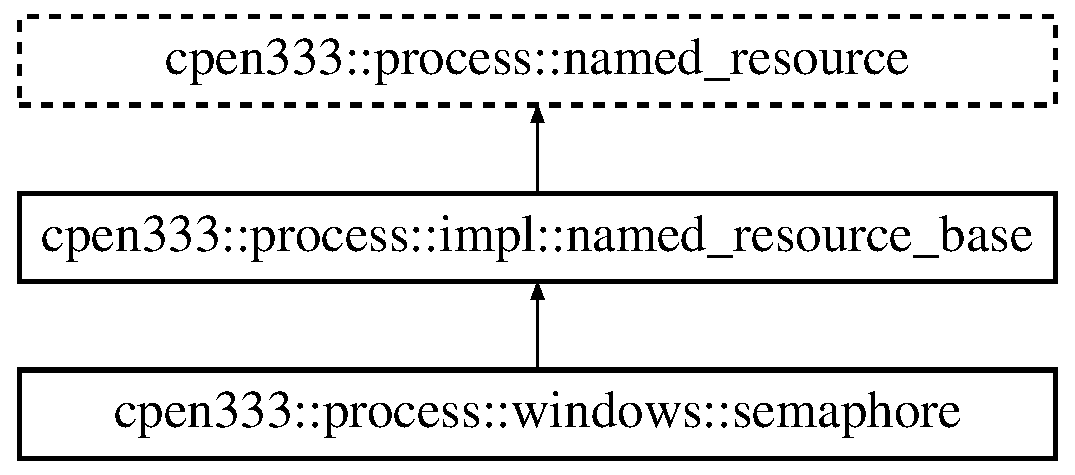
\includegraphics[height=3.000000cm]{classcpen333_1_1process_1_1windows_1_1semaphore}
\end{center}
\end{figure}
\subsection*{Public Types}
\begin{DoxyCompactItemize}
\item 
using \hyperlink{classcpen333_1_1process_1_1windows_1_1semaphore_aa3e5433587a4f60fc2984eb3509946c9}{native\+\_\+handle\+\_\+type} = H\+A\+N\+D\+LE
\begin{DoxyCompactList}\small\item\em Alias to native handle type for semaphore. \end{DoxyCompactList}\end{DoxyCompactItemize}
\subsection*{Public Member Functions}
\begin{DoxyCompactItemize}
\item 
\hyperlink{classcpen333_1_1process_1_1windows_1_1semaphore_a1bd71d0b00c26143be3187c18ec6865a}{semaphore} (const std\+::string \&\hyperlink{classcpen333_1_1process_1_1impl_1_1named__resource__base_ae0c5fbb1843afe863cece4b51c38f807}{name}, size\+\_\+t \hyperlink{classcpen333_1_1process_1_1windows_1_1semaphore_a15245feed98e3cf8a428c0a218f33012}{value}=1)
\begin{DoxyCompactList}\small\item\em Constructs or connects to a named semaphore. \end{DoxyCompactList}\item 
\mbox{\Hypertarget{classcpen333_1_1process_1_1windows_1_1semaphore_a10260478f3b3732d4a52499385ad6575}\label{classcpen333_1_1process_1_1windows_1_1semaphore_a10260478f3b3732d4a52499385ad6575}} 
\hyperlink{classcpen333_1_1process_1_1windows_1_1semaphore_a10260478f3b3732d4a52499385ad6575}{$\sim$semaphore} ()
\begin{DoxyCompactList}\small\item\em Destructor. \end{DoxyCompactList}\item 
size\+\_\+t \hyperlink{classcpen333_1_1process_1_1windows_1_1semaphore_a15245feed98e3cf8a428c0a218f33012}{value} ()
\begin{DoxyCompactList}\small\item\em Determines the current stored value of the semaphore. \end{DoxyCompactList}\item 
void \hyperlink{classcpen333_1_1process_1_1windows_1_1semaphore_a523d89b784ed47ade79d4ecf836f042d}{wait} ()
\begin{DoxyCompactList}\small\item\em Waits for and decrements the semaphore value. \end{DoxyCompactList}\item 
bool \hyperlink{classcpen333_1_1process_1_1windows_1_1semaphore_a06cffd6c2ed120af0477252fb48b0346}{try\+\_\+wait} ()
\begin{DoxyCompactList}\small\item\em Tries to wait for the semaphore, returning immediately. \end{DoxyCompactList}\item 
{\footnotesize template$<$class Rep , class Period $>$ }\\bool \hyperlink{classcpen333_1_1process_1_1windows_1_1semaphore_a055c5a6ec94b231b04856ba78862b0ee}{wait\+\_\+for} (const std\+::chrono\+::duration$<$ Rep, Period $>$ \&timeout\+\_\+duration)
\begin{DoxyCompactList}\small\item\em Tries to wait for the semaphore for up to a maximum timeout duration. \end{DoxyCompactList}\item 
{\footnotesize template$<$class Clock , class Duration $>$ }\\bool \hyperlink{classcpen333_1_1process_1_1windows_1_1semaphore_a2264a9d3557c6507b6c2e37599bd3f83}{wait\+\_\+until} (const std\+::chrono\+::time\+\_\+point$<$ Clock, Duration $>$ \&timeout\+\_\+time)
\begin{DoxyCompactList}\small\item\em Tries to wait for the semaphore for up to a maximum absolute time. \end{DoxyCompactList}\item 
void \hyperlink{classcpen333_1_1process_1_1windows_1_1semaphore_a7f1443d55e1112e7b2a15334bafc958b}{notify} ()
\begin{DoxyCompactList}\small\item\em Increments the semaphore value. \end{DoxyCompactList}\item 
\hyperlink{classcpen333_1_1process_1_1windows_1_1semaphore_aa3e5433587a4f60fc2984eb3509946c9}{native\+\_\+handle\+\_\+type} \hyperlink{classcpen333_1_1process_1_1windows_1_1semaphore_ae73fa406be3b0df603b260e892c94081}{native\+\_\+handle} ()
\begin{DoxyCompactList}\small\item\em Returns a native handle to the semaphore. \end{DoxyCompactList}\item 
bool \hyperlink{classcpen333_1_1process_1_1windows_1_1semaphore_abc5159f32e61024c6c6a978ac64fe39d}{unlink} ()
\begin{DoxyCompactList}\small\item\em Detaches the name from the named resource. \end{DoxyCompactList}\end{DoxyCompactItemize}
\subsection*{Static Public Member Functions}
\begin{DoxyCompactItemize}
\item 
static bool \hyperlink{classcpen333_1_1process_1_1windows_1_1semaphore_ae3837124e878a66370b7e1931c6b1bf8}{unlink} (const std\+::string \&\hyperlink{classcpen333_1_1process_1_1impl_1_1named__resource__base_ae0c5fbb1843afe863cece4b51c38f807}{name})
\begin{DoxyCompactList}\small\item\em Unlinks the name without needing to create a resource. \end{DoxyCompactList}\end{DoxyCompactItemize}
\subsection*{Additional Inherited Members}


\subsection{Detailed Description}
Inter-\/process named semaphore primitive. 

Used to limit access to a number of resources. Contains an integer whose value is never allowed to fall below zero. There are two main supported actions\+: \hyperlink{classcpen333_1_1process_1_1windows_1_1semaphore_a523d89b784ed47ade79d4ecf836f042d}{wait()}, which decrements the internal value, and \hyperlink{classcpen333_1_1process_1_1windows_1_1semaphore_a7f1443d55e1112e7b2a15334bafc958b}{notify()} which increments the value. If the value of the semaphore is zero, then \hyperlink{classcpen333_1_1process_1_1windows_1_1semaphore_a523d89b784ed47ade79d4ecf836f042d}{wait()} will cause the thread to block until the value becomes greater than zero.

This implementation has no explicit maximum value

This semaphore has U\+S\+A\+GE P\+E\+R\+S\+I\+S\+T\+E\+N\+CE, meaning the mutex will continue to exist as long as at least one process/thread is holding a reference to it. 

\subsection{Member Typedef Documentation}
\mbox{\Hypertarget{classcpen333_1_1process_1_1windows_1_1semaphore_aa3e5433587a4f60fc2984eb3509946c9}\label{classcpen333_1_1process_1_1windows_1_1semaphore_aa3e5433587a4f60fc2984eb3509946c9}} 
\index{cpen333\+::process\+::windows\+::semaphore@{cpen333\+::process\+::windows\+::semaphore}!native\+\_\+handle\+\_\+type@{native\+\_\+handle\+\_\+type}}
\index{native\+\_\+handle\+\_\+type@{native\+\_\+handle\+\_\+type}!cpen333\+::process\+::windows\+::semaphore@{cpen333\+::process\+::windows\+::semaphore}}
\subsubsection{\texorpdfstring{native\+\_\+handle\+\_\+type}{native\_handle\_type}}
{\footnotesize\ttfamily using \hyperlink{classcpen333_1_1process_1_1posix_1_1semaphore_ad63150e5c8c196a84a7b214462756f1a}{cpen333\+::process\+::windows\+::semaphore\+::native\+\_\+handle\+\_\+type} =  H\+A\+N\+D\+LE}



Alias to native handle type for semaphore. 

In this case, a Windows H\+A\+N\+D\+LE to a Semaphore 

\subsection{Constructor \& Destructor Documentation}
\mbox{\Hypertarget{classcpen333_1_1process_1_1windows_1_1semaphore_a1bd71d0b00c26143be3187c18ec6865a}\label{classcpen333_1_1process_1_1windows_1_1semaphore_a1bd71d0b00c26143be3187c18ec6865a}} 
\index{cpen333\+::process\+::windows\+::semaphore@{cpen333\+::process\+::windows\+::semaphore}!semaphore@{semaphore}}
\index{semaphore@{semaphore}!cpen333\+::process\+::windows\+::semaphore@{cpen333\+::process\+::windows\+::semaphore}}
\subsubsection{\texorpdfstring{semaphore()}{semaphore()}}
{\footnotesize\ttfamily cpen333\+::process\+::windows\+::semaphore\+::semaphore (\begin{DoxyParamCaption}\item[{const std\+::string \&}]{name,  }\item[{size\+\_\+t}]{value = {\ttfamily 1} }\end{DoxyParamCaption})\hspace{0.3cm}{\ttfamily [inline]}}



Constructs or connects to a named semaphore. 


\begin{DoxyParams}{Parameters}
{\em name} & identifier for creating or connecting to an existing inter-\/process semaphore \\
\hline
{\em value} & initial value (defaults to 1) \\
\hline
\end{DoxyParams}


\subsection{Member Function Documentation}
\mbox{\Hypertarget{classcpen333_1_1process_1_1windows_1_1semaphore_ae73fa406be3b0df603b260e892c94081}\label{classcpen333_1_1process_1_1windows_1_1semaphore_ae73fa406be3b0df603b260e892c94081}} 
\index{cpen333\+::process\+::windows\+::semaphore@{cpen333\+::process\+::windows\+::semaphore}!native\+\_\+handle@{native\+\_\+handle}}
\index{native\+\_\+handle@{native\+\_\+handle}!cpen333\+::process\+::windows\+::semaphore@{cpen333\+::process\+::windows\+::semaphore}}
\subsubsection{\texorpdfstring{native\+\_\+handle()}{native\_handle()}}
{\footnotesize\ttfamily \hyperlink{classcpen333_1_1process_1_1windows_1_1semaphore_aa3e5433587a4f60fc2984eb3509946c9}{native\+\_\+handle\+\_\+type} cpen333\+::process\+::windows\+::semaphore\+::native\+\_\+handle (\begin{DoxyParamCaption}{ }\end{DoxyParamCaption})\hspace{0.3cm}{\ttfamily [inline]}}



Returns a native handle to the semaphore. 

The native handle has a type aliased to \hyperlink{classcpen333_1_1process_1_1windows_1_1semaphore_aa3e5433587a4f60fc2984eb3509946c9}{semaphore\+::native\+\_\+handle\+\_\+type}

On Windows systems, is of type H\+A\+N\+D\+LE to a Semaphore.

\begin{DoxyReturn}{Returns}
native semaphore handle 
\end{DoxyReturn}
\mbox{\Hypertarget{classcpen333_1_1process_1_1windows_1_1semaphore_a7f1443d55e1112e7b2a15334bafc958b}\label{classcpen333_1_1process_1_1windows_1_1semaphore_a7f1443d55e1112e7b2a15334bafc958b}} 
\index{cpen333\+::process\+::windows\+::semaphore@{cpen333\+::process\+::windows\+::semaphore}!notify@{notify}}
\index{notify@{notify}!cpen333\+::process\+::windows\+::semaphore@{cpen333\+::process\+::windows\+::semaphore}}
\subsubsection{\texorpdfstring{notify()}{notify()}}
{\footnotesize\ttfamily void cpen333\+::process\+::windows\+::semaphore\+::notify (\begin{DoxyParamCaption}{ }\end{DoxyParamCaption})\hspace{0.3cm}{\ttfamily [inline]}}



Increments the semaphore value. 

If the semaphore\textquotesingle{}s value consequently becomes greater than zero, then one process or thread that is currently blocked in a \hyperlink{classcpen333_1_1process_1_1windows_1_1semaphore_a523d89b784ed47ade79d4ecf836f042d}{wait()} operation will be woken up and will proceed. \mbox{\Hypertarget{classcpen333_1_1process_1_1windows_1_1semaphore_a06cffd6c2ed120af0477252fb48b0346}\label{classcpen333_1_1process_1_1windows_1_1semaphore_a06cffd6c2ed120af0477252fb48b0346}} 
\index{cpen333\+::process\+::windows\+::semaphore@{cpen333\+::process\+::windows\+::semaphore}!try\+\_\+wait@{try\+\_\+wait}}
\index{try\+\_\+wait@{try\+\_\+wait}!cpen333\+::process\+::windows\+::semaphore@{cpen333\+::process\+::windows\+::semaphore}}
\subsubsection{\texorpdfstring{try\+\_\+wait()}{try\_wait()}}
{\footnotesize\ttfamily bool cpen333\+::process\+::windows\+::semaphore\+::try\+\_\+wait (\begin{DoxyParamCaption}{ }\end{DoxyParamCaption})\hspace{0.3cm}{\ttfamily [inline]}}



Tries to wait for the semaphore, returning immediately. 

If the value is greater than zero, will decrement the semaphore and return true. Otherwise, will return false.

\begin{DoxyReturn}{Returns}
true if decrement successful, false otherwise 
\end{DoxyReturn}
\mbox{\Hypertarget{classcpen333_1_1process_1_1windows_1_1semaphore_abc5159f32e61024c6c6a978ac64fe39d}\label{classcpen333_1_1process_1_1windows_1_1semaphore_abc5159f32e61024c6c6a978ac64fe39d}} 
\index{cpen333\+::process\+::windows\+::semaphore@{cpen333\+::process\+::windows\+::semaphore}!unlink@{unlink}}
\index{unlink@{unlink}!cpen333\+::process\+::windows\+::semaphore@{cpen333\+::process\+::windows\+::semaphore}}
\subsubsection{\texorpdfstring{unlink()}{unlink()}\hspace{0.1cm}{\footnotesize\ttfamily [1/2]}}
{\footnotesize\ttfamily bool cpen333\+::process\+::windows\+::semaphore\+::unlink (\begin{DoxyParamCaption}{ }\end{DoxyParamCaption})\hspace{0.3cm}{\ttfamily [inline]}, {\ttfamily [virtual]}}



Detaches the name from the named resource. 

On P\+O\+S\+IX systems, named resources will persist beyond the lifetime of any process that uses them as long as the name has not been unlinked (or until the system is rebooted). Calling {\ttfamily unlink} will detach the name, allowing the resource to be freed once all current users have exited.

\begin{DoxyReturn}{Returns}
{\ttfamily true} if unlink is successful, {\ttfamily false} if unlinking is not supported or if an error has occurred. 
\end{DoxyReturn}


Implements \hyperlink{classcpen333_1_1process_1_1impl_1_1named__resource__base_ae4033f82dfd068b917a9bca57d3a0c45}{cpen333\+::process\+::impl\+::named\+\_\+resource\+\_\+base}.

\mbox{\Hypertarget{classcpen333_1_1process_1_1windows_1_1semaphore_ae3837124e878a66370b7e1931c6b1bf8}\label{classcpen333_1_1process_1_1windows_1_1semaphore_ae3837124e878a66370b7e1931c6b1bf8}} 
\index{cpen333\+::process\+::windows\+::semaphore@{cpen333\+::process\+::windows\+::semaphore}!unlink@{unlink}}
\index{unlink@{unlink}!cpen333\+::process\+::windows\+::semaphore@{cpen333\+::process\+::windows\+::semaphore}}
\subsubsection{\texorpdfstring{unlink()}{unlink()}\hspace{0.1cm}{\footnotesize\ttfamily [2/2]}}
{\footnotesize\ttfamily static bool cpen333\+::process\+::windows\+::semaphore\+::unlink (\begin{DoxyParamCaption}\item[{const std\+::string \&}]{name }\end{DoxyParamCaption})\hspace{0.3cm}{\ttfamily [inline]}, {\ttfamily [static]}}



Unlinks the name without needing to create a resource. 

Implementers should also provide a static method for unlinking. The purpose is mainly for clean-\/up of existing resources.


\begin{DoxyParams}{Parameters}
{\em name} & desired resource name \\
\hline
\end{DoxyParams}
\begin{DoxyReturn}{Returns}
{\ttfamily true} if unlink successful, {\ttfamily false} if not successful or not supported 
\end{DoxyReturn}
\mbox{\Hypertarget{classcpen333_1_1process_1_1windows_1_1semaphore_a15245feed98e3cf8a428c0a218f33012}\label{classcpen333_1_1process_1_1windows_1_1semaphore_a15245feed98e3cf8a428c0a218f33012}} 
\index{cpen333\+::process\+::windows\+::semaphore@{cpen333\+::process\+::windows\+::semaphore}!value@{value}}
\index{value@{value}!cpen333\+::process\+::windows\+::semaphore@{cpen333\+::process\+::windows\+::semaphore}}
\subsubsection{\texorpdfstring{value()}{value()}}
{\footnotesize\ttfamily size\+\_\+t cpen333\+::process\+::windows\+::semaphore\+::value (\begin{DoxyParamCaption}{ }\end{DoxyParamCaption})\hspace{0.3cm}{\ttfamily [inline]}}



Determines the current stored value of the semaphore. 

This should never be used, except for possibly debugging, as the value may change without notice from other threads. This method will cause an error on O\+SX.

\begin{DoxyReturn}{Returns}

\end{DoxyReturn}
\mbox{\Hypertarget{classcpen333_1_1process_1_1windows_1_1semaphore_a523d89b784ed47ade79d4ecf836f042d}\label{classcpen333_1_1process_1_1windows_1_1semaphore_a523d89b784ed47ade79d4ecf836f042d}} 
\index{cpen333\+::process\+::windows\+::semaphore@{cpen333\+::process\+::windows\+::semaphore}!wait@{wait}}
\index{wait@{wait}!cpen333\+::process\+::windows\+::semaphore@{cpen333\+::process\+::windows\+::semaphore}}
\subsubsection{\texorpdfstring{wait()}{wait()}}
{\footnotesize\ttfamily void cpen333\+::process\+::windows\+::semaphore\+::wait (\begin{DoxyParamCaption}{ }\end{DoxyParamCaption})\hspace{0.3cm}{\ttfamily [inline]}}



Waits for and decrements the semaphore value. 

If the value is greater than zero, will decrement it and return immediately. Otherwise, the thread will block until it becomes possible to perform the decrement. \mbox{\Hypertarget{classcpen333_1_1process_1_1windows_1_1semaphore_a055c5a6ec94b231b04856ba78862b0ee}\label{classcpen333_1_1process_1_1windows_1_1semaphore_a055c5a6ec94b231b04856ba78862b0ee}} 
\index{cpen333\+::process\+::windows\+::semaphore@{cpen333\+::process\+::windows\+::semaphore}!wait\+\_\+for@{wait\+\_\+for}}
\index{wait\+\_\+for@{wait\+\_\+for}!cpen333\+::process\+::windows\+::semaphore@{cpen333\+::process\+::windows\+::semaphore}}
\subsubsection{\texorpdfstring{wait\+\_\+for()}{wait\_for()}}
{\footnotesize\ttfamily template$<$class Rep , class Period $>$ \\
bool cpen333\+::process\+::windows\+::semaphore\+::wait\+\_\+for (\begin{DoxyParamCaption}\item[{const std\+::chrono\+::duration$<$ Rep, Period $>$ \&}]{timeout\+\_\+duration }\end{DoxyParamCaption})\hspace{0.3cm}{\ttfamily [inline]}}



Tries to wait for the semaphore for up to a maximum timeout duration. 

If the semaphore\textquotesingle{}s value is greater than zero, will decrement it and return true immediately. Otherwise, will wait (blocking) up to a maximum relative timeout period.


\begin{DoxyTemplParams}{Template Parameters}
{\em Rep} & time representation \\
\hline
{\em Period} & timeout period type \\
\hline
\end{DoxyTemplParams}

\begin{DoxyParams}{Parameters}
{\em timeout\+\_\+duration} & maximum relative duration for waiting \\
\hline
\end{DoxyParams}
\begin{DoxyReturn}{Returns}
true if semaphore successfully decremented, false if timed-\/out 
\end{DoxyReturn}
\mbox{\Hypertarget{classcpen333_1_1process_1_1windows_1_1semaphore_a2264a9d3557c6507b6c2e37599bd3f83}\label{classcpen333_1_1process_1_1windows_1_1semaphore_a2264a9d3557c6507b6c2e37599bd3f83}} 
\index{cpen333\+::process\+::windows\+::semaphore@{cpen333\+::process\+::windows\+::semaphore}!wait\+\_\+until@{wait\+\_\+until}}
\index{wait\+\_\+until@{wait\+\_\+until}!cpen333\+::process\+::windows\+::semaphore@{cpen333\+::process\+::windows\+::semaphore}}
\subsubsection{\texorpdfstring{wait\+\_\+until()}{wait\_until()}}
{\footnotesize\ttfamily template$<$class Clock , class Duration $>$ \\
bool cpen333\+::process\+::windows\+::semaphore\+::wait\+\_\+until (\begin{DoxyParamCaption}\item[{const std\+::chrono\+::time\+\_\+point$<$ Clock, Duration $>$ \&}]{timeout\+\_\+time }\end{DoxyParamCaption})\hspace{0.3cm}{\ttfamily [inline]}}



Tries to wait for the semaphore for up to a maximum absolute time. 

If the semaphore\textquotesingle{}s value is greater than zero, will decrement it and return true immediately. Otherwise, will wait (blocking) up to a maximum relative timeout period.


\begin{DoxyTemplParams}{Template Parameters}
{\em Clock} & timeout clock type \\
\hline
{\em Duration} & timeout duration type \\
\hline
\end{DoxyTemplParams}

\begin{DoxyParams}{Parameters}
{\em timeout\+\_\+time} & maximum absolute time for waiting \\
\hline
\end{DoxyParams}
\begin{DoxyReturn}{Returns}
true if semaphore successfully decremented, false if timed-\/out 
\end{DoxyReturn}


The documentation for this class was generated from the following file\+:\begin{DoxyCompactItemize}
\item 
D\+:/school/teaching/\+C\+P\+E\+N333/workspace/labs/include/cpen333/process/impl/windows/\hyperlink{process_2impl_2windows_2semaphore_8h}{semaphore.\+h}\end{DoxyCompactItemize}

\hypertarget{classcpen333_1_1process_1_1semaphore}{}\section{cpen333\+:\+:process\+:\+:semaphore Class Reference}
\label{classcpen333_1_1process_1_1semaphore}\index{cpen333\+::process\+::semaphore@{cpen333\+::process\+::semaphore}}


An inter-\/process semaphore synchronization primitive.  




{\ttfamily \#include $<$semaphore.\+h$>$}



\subsection{Detailed Description}
An inter-\/process semaphore synchronization primitive. 

Used to protect access to a counted resource shared by multiple processes. This is an alias to either \hyperlink{classcpen333_1_1process_1_1posix_1_1semaphore}{cpen333\+::process\+::posix\+::semaphore} or \hyperlink{classcpen333_1_1process_1_1windows_1_1semaphore}{cpen333\+::process\+::windows\+::semaphore} depending on your platform. 

The documentation for this class was generated from the following file\+:\begin{DoxyCompactItemize}
\item 
D\+:/school/teaching/\+C\+P\+E\+N333/workspace/library/include/cpen333/process/\hyperlink{process_2semaphore_8h}{semaphore.\+h}\end{DoxyCompactItemize}

\hypertarget{classcpen333_1_1process_1_1posix_1_1semaphore}{}\section{cpen333\+:\+:process\+:\+:posix\+:\+:semaphore Class Reference}
\label{classcpen333_1_1process_1_1posix_1_1semaphore}\index{cpen333\+::process\+::posix\+::semaphore@{cpen333\+::process\+::posix\+::semaphore}}


Inter-\/process named semaphore primitive.  




{\ttfamily \#include $<$semaphore.\+h$>$}

Inheritance diagram for cpen333\+:\+:process\+:\+:posix\+:\+:semaphore\+:\begin{figure}[H]
\begin{center}
\leavevmode
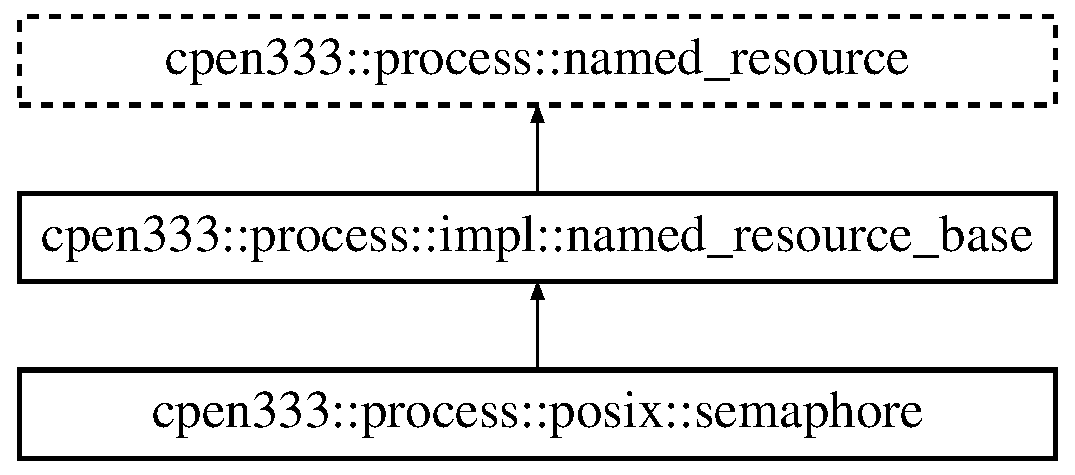
\includegraphics[height=3.000000cm]{classcpen333_1_1process_1_1posix_1_1semaphore}
\end{center}
\end{figure}
\subsection*{Public Types}
\begin{DoxyCompactItemize}
\item 
using \hyperlink{classcpen333_1_1process_1_1posix_1_1semaphore_ad63150e5c8c196a84a7b214462756f1a}{native\+\_\+handle\+\_\+type} = sem\+\_\+t $\ast$
\begin{DoxyCompactList}\small\item\em Alias to native handle type for semaphore. \end{DoxyCompactList}\end{DoxyCompactItemize}
\subsection*{Public Member Functions}
\begin{DoxyCompactItemize}
\item 
\hyperlink{classcpen333_1_1process_1_1posix_1_1semaphore_aee6d65abd5bbfcfd1629140cb20c8ad1}{semaphore} (const std\+::string \&\hyperlink{classcpen333_1_1process_1_1impl_1_1named__resource__base_ae0c5fbb1843afe863cece4b51c38f807}{name}, size\+\_\+t \hyperlink{classcpen333_1_1process_1_1posix_1_1semaphore_a336211ff42ee9da6315c76104840fa98}{value}=1)
\begin{DoxyCompactList}\small\item\em Constructs or connects to a named semaphore. \end{DoxyCompactList}\item 
\mbox{\Hypertarget{classcpen333_1_1process_1_1posix_1_1semaphore_a9c32f8d2192cca78b7415f9e3af056a6}\label{classcpen333_1_1process_1_1posix_1_1semaphore_a9c32f8d2192cca78b7415f9e3af056a6}} 
\hyperlink{classcpen333_1_1process_1_1posix_1_1semaphore_a9c32f8d2192cca78b7415f9e3af056a6}{$\sim$semaphore} ()
\begin{DoxyCompactList}\small\item\em Destructor. \end{DoxyCompactList}\item 
size\+\_\+t \hyperlink{classcpen333_1_1process_1_1posix_1_1semaphore_a336211ff42ee9da6315c76104840fa98}{value} ()
\begin{DoxyCompactList}\small\item\em Determines the current stored value of the semaphore. \end{DoxyCompactList}\item 
void \hyperlink{classcpen333_1_1process_1_1posix_1_1semaphore_a1cf2d5f5922ab6358061dd3ac7121cf9}{wait} ()
\begin{DoxyCompactList}\small\item\em Waits for and decrements the semaphore value. \end{DoxyCompactList}\item 
bool \hyperlink{classcpen333_1_1process_1_1posix_1_1semaphore_ac0e2bd6495113c0699c5e2511f345edb}{try\+\_\+wait} ()
\begin{DoxyCompactList}\small\item\em Tries to wait for the semaphore, returning immediately. \end{DoxyCompactList}\item 
void \hyperlink{classcpen333_1_1process_1_1posix_1_1semaphore_a1b9043106c5da18ad152bc83e3de1750}{notify} ()
\begin{DoxyCompactList}\small\item\em Increments the semaphore value. \end{DoxyCompactList}\item 
{\footnotesize template$<$class Rep , class Period $>$ }\\bool \hyperlink{classcpen333_1_1process_1_1posix_1_1semaphore_a8015c878067c3d93748d03c58bb1b233}{wait\+\_\+for} (const std\+::chrono\+::duration$<$ Rep, Period $>$ \&timeout\+\_\+duration)
\begin{DoxyCompactList}\small\item\em Tries to wait for the semaphore for up to a maximum timeout duration. \end{DoxyCompactList}\item 
{\footnotesize template$<$class Clock , class Duration $>$ }\\bool \hyperlink{classcpen333_1_1process_1_1posix_1_1semaphore_a83443f24c1b7b11e5384975e9abc77dc}{wait\+\_\+until} (const std\+::chrono\+::time\+\_\+point$<$ Clock, Duration $>$ \&timeout\+\_\+time)
\begin{DoxyCompactList}\small\item\em Tries to wait for the semaphore for up to a maximum absolute time. \end{DoxyCompactList}\item 
\hyperlink{classcpen333_1_1process_1_1posix_1_1semaphore_ad63150e5c8c196a84a7b214462756f1a}{native\+\_\+handle\+\_\+type} \hyperlink{classcpen333_1_1process_1_1posix_1_1semaphore_a1e4a2d5a032a71fc06a5065f0e83a94c}{native\+\_\+handle} () const
\begin{DoxyCompactList}\small\item\em Returns a native handle to the semaphore. \end{DoxyCompactList}\item 
bool \hyperlink{classcpen333_1_1process_1_1posix_1_1semaphore_aa6064e2c4b4b7282cc5e6eda877ee1bb}{unlink} ()
\begin{DoxyCompactList}\small\item\em Detaches the name from the named resource. \end{DoxyCompactList}\end{DoxyCompactItemize}
\subsection*{Static Public Member Functions}
\begin{DoxyCompactItemize}
\item 
static bool \hyperlink{classcpen333_1_1process_1_1posix_1_1semaphore_ab1399175014f674484217be6d465e878}{unlink} (const std\+::string \&\hyperlink{classcpen333_1_1process_1_1impl_1_1named__resource__base_ae0c5fbb1843afe863cece4b51c38f807}{name})
\begin{DoxyCompactList}\small\item\em Unlinks the name without needing to create a resource. \end{DoxyCompactList}\end{DoxyCompactItemize}
\subsection*{Additional Inherited Members}


\subsection{Detailed Description}
Inter-\/process named semaphore primitive. 

Used to limit access to a number of resources. Contains an integer whose value is never allowed to fall below zero. There are two main supported actions\+: \hyperlink{classcpen333_1_1process_1_1posix_1_1semaphore_a1cf2d5f5922ab6358061dd3ac7121cf9}{wait()}, which decrements the internal value, and \hyperlink{classcpen333_1_1process_1_1posix_1_1semaphore_a1b9043106c5da18ad152bc83e3de1750}{notify()} which increments the value. If the value of the semaphore is zero, then \hyperlink{classcpen333_1_1process_1_1posix_1_1semaphore_a1cf2d5f5922ab6358061dd3ac7121cf9}{wait()} will cause the thread to block until the value becomes greater than zero.

This implementation has no explicit maximum value

This semaphore has K\+E\+R\+N\+EL P\+E\+R\+S\+I\+S\+T\+E\+N\+CE, meaning if not \hyperlink{classcpen333_1_1process_1_1posix_1_1semaphore_aa6064e2c4b4b7282cc5e6eda877ee1bb}{unlink()}-\/ed, will continue to exist in its current state until the system is shut down (persisting beyond the life of the initiating program) 

\subsection{Member Typedef Documentation}
\mbox{\Hypertarget{classcpen333_1_1process_1_1posix_1_1semaphore_ad63150e5c8c196a84a7b214462756f1a}\label{classcpen333_1_1process_1_1posix_1_1semaphore_ad63150e5c8c196a84a7b214462756f1a}} 
\index{cpen333\+::process\+::posix\+::semaphore@{cpen333\+::process\+::posix\+::semaphore}!native\+\_\+handle\+\_\+type@{native\+\_\+handle\+\_\+type}}
\index{native\+\_\+handle\+\_\+type@{native\+\_\+handle\+\_\+type}!cpen333\+::process\+::posix\+::semaphore@{cpen333\+::process\+::posix\+::semaphore}}
\subsubsection{\texorpdfstring{native\+\_\+handle\+\_\+type}{native\_handle\_type}}
{\footnotesize\ttfamily using \hyperlink{classcpen333_1_1process_1_1posix_1_1semaphore_ad63150e5c8c196a84a7b214462756f1a}{cpen333\+::process\+::posix\+::semaphore\+::native\+\_\+handle\+\_\+type} =  sem\+\_\+t$\ast$}



Alias to native handle type for semaphore. 

In this case, a P\+O\+S\+IX sem\+\_\+t$\ast$ 

\subsection{Constructor \& Destructor Documentation}
\mbox{\Hypertarget{classcpen333_1_1process_1_1posix_1_1semaphore_aee6d65abd5bbfcfd1629140cb20c8ad1}\label{classcpen333_1_1process_1_1posix_1_1semaphore_aee6d65abd5bbfcfd1629140cb20c8ad1}} 
\index{cpen333\+::process\+::posix\+::semaphore@{cpen333\+::process\+::posix\+::semaphore}!semaphore@{semaphore}}
\index{semaphore@{semaphore}!cpen333\+::process\+::posix\+::semaphore@{cpen333\+::process\+::posix\+::semaphore}}
\subsubsection{\texorpdfstring{semaphore()}{semaphore()}}
{\footnotesize\ttfamily cpen333\+::process\+::posix\+::semaphore\+::semaphore (\begin{DoxyParamCaption}\item[{const std\+::string \&}]{name,  }\item[{size\+\_\+t}]{value = {\ttfamily 1} }\end{DoxyParamCaption})\hspace{0.3cm}{\ttfamily [inline]}}



Constructs or connects to a named semaphore. 


\begin{DoxyParams}{Parameters}
{\em name} & identifier for creating or connecting to an existing inter-\/process semaphore \\
\hline
{\em value} & initial value (defaults to 1) \\
\hline
\end{DoxyParams}


\subsection{Member Function Documentation}
\mbox{\Hypertarget{classcpen333_1_1process_1_1posix_1_1semaphore_a1e4a2d5a032a71fc06a5065f0e83a94c}\label{classcpen333_1_1process_1_1posix_1_1semaphore_a1e4a2d5a032a71fc06a5065f0e83a94c}} 
\index{cpen333\+::process\+::posix\+::semaphore@{cpen333\+::process\+::posix\+::semaphore}!native\+\_\+handle@{native\+\_\+handle}}
\index{native\+\_\+handle@{native\+\_\+handle}!cpen333\+::process\+::posix\+::semaphore@{cpen333\+::process\+::posix\+::semaphore}}
\subsubsection{\texorpdfstring{native\+\_\+handle()}{native\_handle()}}
{\footnotesize\ttfamily \hyperlink{classcpen333_1_1process_1_1posix_1_1semaphore_ad63150e5c8c196a84a7b214462756f1a}{native\+\_\+handle\+\_\+type} cpen333\+::process\+::posix\+::semaphore\+::native\+\_\+handle (\begin{DoxyParamCaption}{ }\end{DoxyParamCaption}) const\hspace{0.3cm}{\ttfamily [inline]}}



Returns a native handle to the semaphore. 

The native handle has a type aliased to \hyperlink{classcpen333_1_1process_1_1posix_1_1semaphore_ad63150e5c8c196a84a7b214462756f1a}{semaphore\+::native\+\_\+handle\+\_\+type}

On P\+O\+S\+IX systems, is of type sem\+\_\+t$\ast$.

\begin{DoxyReturn}{Returns}
native semaphore handle 
\end{DoxyReturn}
\mbox{\Hypertarget{classcpen333_1_1process_1_1posix_1_1semaphore_a1b9043106c5da18ad152bc83e3de1750}\label{classcpen333_1_1process_1_1posix_1_1semaphore_a1b9043106c5da18ad152bc83e3de1750}} 
\index{cpen333\+::process\+::posix\+::semaphore@{cpen333\+::process\+::posix\+::semaphore}!notify@{notify}}
\index{notify@{notify}!cpen333\+::process\+::posix\+::semaphore@{cpen333\+::process\+::posix\+::semaphore}}
\subsubsection{\texorpdfstring{notify()}{notify()}}
{\footnotesize\ttfamily void cpen333\+::process\+::posix\+::semaphore\+::notify (\begin{DoxyParamCaption}{ }\end{DoxyParamCaption})\hspace{0.3cm}{\ttfamily [inline]}}



Increments the semaphore value. 

If the semaphore\textquotesingle{}s value consequently becomes greater than zero, then one process or thread that is currently blocked in a \hyperlink{classcpen333_1_1process_1_1posix_1_1semaphore_a1cf2d5f5922ab6358061dd3ac7121cf9}{wait()} operation will be woken up and will proceed. \mbox{\Hypertarget{classcpen333_1_1process_1_1posix_1_1semaphore_ac0e2bd6495113c0699c5e2511f345edb}\label{classcpen333_1_1process_1_1posix_1_1semaphore_ac0e2bd6495113c0699c5e2511f345edb}} 
\index{cpen333\+::process\+::posix\+::semaphore@{cpen333\+::process\+::posix\+::semaphore}!try\+\_\+wait@{try\+\_\+wait}}
\index{try\+\_\+wait@{try\+\_\+wait}!cpen333\+::process\+::posix\+::semaphore@{cpen333\+::process\+::posix\+::semaphore}}
\subsubsection{\texorpdfstring{try\+\_\+wait()}{try\_wait()}}
{\footnotesize\ttfamily bool cpen333\+::process\+::posix\+::semaphore\+::try\+\_\+wait (\begin{DoxyParamCaption}{ }\end{DoxyParamCaption})\hspace{0.3cm}{\ttfamily [inline]}}



Tries to wait for the semaphore, returning immediately. 

If the value is greater than zero, will decrement the semaphore and return true. Otherwise, will return false.

\begin{DoxyReturn}{Returns}
true if decrement successful, false otherwise 
\end{DoxyReturn}
\mbox{\Hypertarget{classcpen333_1_1process_1_1posix_1_1semaphore_aa6064e2c4b4b7282cc5e6eda877ee1bb}\label{classcpen333_1_1process_1_1posix_1_1semaphore_aa6064e2c4b4b7282cc5e6eda877ee1bb}} 
\index{cpen333\+::process\+::posix\+::semaphore@{cpen333\+::process\+::posix\+::semaphore}!unlink@{unlink}}
\index{unlink@{unlink}!cpen333\+::process\+::posix\+::semaphore@{cpen333\+::process\+::posix\+::semaphore}}
\subsubsection{\texorpdfstring{unlink()}{unlink()}\hspace{0.1cm}{\footnotesize\ttfamily [1/2]}}
{\footnotesize\ttfamily bool cpen333\+::process\+::posix\+::semaphore\+::unlink (\begin{DoxyParamCaption}{ }\end{DoxyParamCaption})\hspace{0.3cm}{\ttfamily [inline]}, {\ttfamily [virtual]}}



Detaches the name from the named resource. 

On P\+O\+S\+IX systems, named resources will persist beyond the lifetime of any process that uses them as long as the name has not been unlinked (or until the system is rebooted). Calling {\ttfamily unlink} will detach the name, allowing the resource to be freed once all current users have exited.

\begin{DoxyReturn}{Returns}
{\ttfamily true} if unlink is successful, {\ttfamily false} if unlinking is not supported or if an error has occurred. 
\end{DoxyReturn}


Implements \hyperlink{classcpen333_1_1process_1_1impl_1_1named__resource__base_ae4033f82dfd068b917a9bca57d3a0c45}{cpen333\+::process\+::impl\+::named\+\_\+resource\+\_\+base}.

\mbox{\Hypertarget{classcpen333_1_1process_1_1posix_1_1semaphore_ab1399175014f674484217be6d465e878}\label{classcpen333_1_1process_1_1posix_1_1semaphore_ab1399175014f674484217be6d465e878}} 
\index{cpen333\+::process\+::posix\+::semaphore@{cpen333\+::process\+::posix\+::semaphore}!unlink@{unlink}}
\index{unlink@{unlink}!cpen333\+::process\+::posix\+::semaphore@{cpen333\+::process\+::posix\+::semaphore}}
\subsubsection{\texorpdfstring{unlink()}{unlink()}\hspace{0.1cm}{\footnotesize\ttfamily [2/2]}}
{\footnotesize\ttfamily static bool cpen333\+::process\+::posix\+::semaphore\+::unlink (\begin{DoxyParamCaption}\item[{const std\+::string \&}]{name }\end{DoxyParamCaption})\hspace{0.3cm}{\ttfamily [inline]}, {\ttfamily [static]}}



Unlinks the name without needing to create a resource. 

Implementers should also provide a static method for unlinking. The purpose is mainly for clean-\/up of existing resources.


\begin{DoxyParams}{Parameters}
{\em name} & desired resource name \\
\hline
\end{DoxyParams}
\begin{DoxyReturn}{Returns}
{\ttfamily true} if unlink successful, {\ttfamily false} if not successful or not supported 
\end{DoxyReturn}
\mbox{\Hypertarget{classcpen333_1_1process_1_1posix_1_1semaphore_a336211ff42ee9da6315c76104840fa98}\label{classcpen333_1_1process_1_1posix_1_1semaphore_a336211ff42ee9da6315c76104840fa98}} 
\index{cpen333\+::process\+::posix\+::semaphore@{cpen333\+::process\+::posix\+::semaphore}!value@{value}}
\index{value@{value}!cpen333\+::process\+::posix\+::semaphore@{cpen333\+::process\+::posix\+::semaphore}}
\subsubsection{\texorpdfstring{value()}{value()}}
{\footnotesize\ttfamily size\+\_\+t cpen333\+::process\+::posix\+::semaphore\+::value (\begin{DoxyParamCaption}{ }\end{DoxyParamCaption})\hspace{0.3cm}{\ttfamily [inline]}}



Determines the current stored value of the semaphore. 

This should never be used, except for possibly debugging, as the value may change without notice from other threads. This method will cause an error on O\+SX.

\begin{DoxyReturn}{Returns}

\end{DoxyReturn}
\mbox{\Hypertarget{classcpen333_1_1process_1_1posix_1_1semaphore_a1cf2d5f5922ab6358061dd3ac7121cf9}\label{classcpen333_1_1process_1_1posix_1_1semaphore_a1cf2d5f5922ab6358061dd3ac7121cf9}} 
\index{cpen333\+::process\+::posix\+::semaphore@{cpen333\+::process\+::posix\+::semaphore}!wait@{wait}}
\index{wait@{wait}!cpen333\+::process\+::posix\+::semaphore@{cpen333\+::process\+::posix\+::semaphore}}
\subsubsection{\texorpdfstring{wait()}{wait()}}
{\footnotesize\ttfamily void cpen333\+::process\+::posix\+::semaphore\+::wait (\begin{DoxyParamCaption}{ }\end{DoxyParamCaption})\hspace{0.3cm}{\ttfamily [inline]}}



Waits for and decrements the semaphore value. 

If the value is greater than zero, will decrement it and return immediately. Otherwise, the thread will block until it becomes possible to perform the decrement. \mbox{\Hypertarget{classcpen333_1_1process_1_1posix_1_1semaphore_a8015c878067c3d93748d03c58bb1b233}\label{classcpen333_1_1process_1_1posix_1_1semaphore_a8015c878067c3d93748d03c58bb1b233}} 
\index{cpen333\+::process\+::posix\+::semaphore@{cpen333\+::process\+::posix\+::semaphore}!wait\+\_\+for@{wait\+\_\+for}}
\index{wait\+\_\+for@{wait\+\_\+for}!cpen333\+::process\+::posix\+::semaphore@{cpen333\+::process\+::posix\+::semaphore}}
\subsubsection{\texorpdfstring{wait\+\_\+for()}{wait\_for()}}
{\footnotesize\ttfamily template$<$class Rep , class Period $>$ \\
bool cpen333\+::process\+::posix\+::semaphore\+::wait\+\_\+for (\begin{DoxyParamCaption}\item[{const std\+::chrono\+::duration$<$ Rep, Period $>$ \&}]{timeout\+\_\+duration }\end{DoxyParamCaption})\hspace{0.3cm}{\ttfamily [inline]}}



Tries to wait for the semaphore for up to a maximum timeout duration. 

If the semaphore\textquotesingle{}s value is greater than zero, will decrement it and return true immediately. Otherwise, will wait (blocking) up to a maximum relative timeout period.


\begin{DoxyTemplParams}{Template Parameters}
{\em Rep} & time representation \\
\hline
{\em Period} & timeout period type \\
\hline
\end{DoxyTemplParams}

\begin{DoxyParams}{Parameters}
{\em timeout\+\_\+duration} & maximum relative duration for waiting \\
\hline
\end{DoxyParams}
\begin{DoxyReturn}{Returns}
true if semaphore successfully decremented, false if timed-\/out 
\end{DoxyReturn}
\mbox{\Hypertarget{classcpen333_1_1process_1_1posix_1_1semaphore_a83443f24c1b7b11e5384975e9abc77dc}\label{classcpen333_1_1process_1_1posix_1_1semaphore_a83443f24c1b7b11e5384975e9abc77dc}} 
\index{cpen333\+::process\+::posix\+::semaphore@{cpen333\+::process\+::posix\+::semaphore}!wait\+\_\+until@{wait\+\_\+until}}
\index{wait\+\_\+until@{wait\+\_\+until}!cpen333\+::process\+::posix\+::semaphore@{cpen333\+::process\+::posix\+::semaphore}}
\subsubsection{\texorpdfstring{wait\+\_\+until()}{wait\_until()}}
{\footnotesize\ttfamily template$<$class Clock , class Duration $>$ \\
bool cpen333\+::process\+::posix\+::semaphore\+::wait\+\_\+until (\begin{DoxyParamCaption}\item[{const std\+::chrono\+::time\+\_\+point$<$ Clock, Duration $>$ \&}]{timeout\+\_\+time }\end{DoxyParamCaption})\hspace{0.3cm}{\ttfamily [inline]}}



Tries to wait for the semaphore for up to a maximum absolute time. 

If the semaphore\textquotesingle{}s value is greater than zero, will decrement it and return true immediately. Otherwise, will wait (blocking) up to a maximum relative timeout period.


\begin{DoxyTemplParams}{Template Parameters}
{\em Clock} & timeout clock type \\
\hline
{\em Duration} & timeout duration type \\
\hline
\end{DoxyTemplParams}

\begin{DoxyParams}{Parameters}
{\em timeout\+\_\+time} & maximum absolute time for waiting \\
\hline
\end{DoxyParams}
\begin{DoxyReturn}{Returns}
true if semaphore successfully decremented, false if timed-\/out 
\end{DoxyReturn}


The documentation for this class was generated from the following file\+:\begin{DoxyCompactItemize}
\item 
D\+:/school/teaching/\+C\+P\+E\+N333/workspace/library/include/cpen333/process/impl/posix/\hyperlink{process_2impl_2posix_2semaphore_8h}{semaphore.\+h}\end{DoxyCompactItemize}

\hypertarget{classcpen333_1_1process_1_1semaphore__guard}{}\section{cpen333\+:\+:process\+:\+:semaphore\+\_\+guard$<$ Semaphore $>$ Class Template Reference}
\label{classcpen333_1_1process_1_1semaphore__guard}\index{cpen333\+::process\+::semaphore\+\_\+guard$<$ Semaphore $>$@{cpen333\+::process\+::semaphore\+\_\+guard$<$ Semaphore $>$}}


Semaphore guard, similar to std\+::lock\+\_\+guard.  




{\ttfamily \#include $<$semaphore\+\_\+guard.\+h$>$}

\subsection*{Public Member Functions}
\begin{DoxyCompactItemize}
\item 
\hyperlink{classcpen333_1_1process_1_1semaphore__guard_aa816ac26e4894b1945724944e7965968}{semaphore\+\_\+guard} (Semaphore \&sem)
\begin{DoxyCompactList}\small\item\em Constructor, waits on semaphore. \end{DoxyCompactList}\item 
\mbox{\Hypertarget{classcpen333_1_1process_1_1semaphore__guard_a12dd43fa23381e3a44eabc8e8d1b55a9}\label{classcpen333_1_1process_1_1semaphore__guard_a12dd43fa23381e3a44eabc8e8d1b55a9}} 
{\bfseries semaphore\+\_\+guard} (const \hyperlink{classcpen333_1_1process_1_1semaphore__guard}{semaphore\+\_\+guard} \&)=delete
\item 
\mbox{\Hypertarget{classcpen333_1_1process_1_1semaphore__guard_a8e970b86d9083bcdfa2ec74950580c41}\label{classcpen333_1_1process_1_1semaphore__guard_a8e970b86d9083bcdfa2ec74950580c41}} 
{\bfseries semaphore\+\_\+guard} (\hyperlink{classcpen333_1_1process_1_1semaphore__guard}{semaphore\+\_\+guard} \&\&)=delete
\item 
\mbox{\Hypertarget{classcpen333_1_1process_1_1semaphore__guard_aa500d54d3674dedc78b6ba2997244690}\label{classcpen333_1_1process_1_1semaphore__guard_aa500d54d3674dedc78b6ba2997244690}} 
\hyperlink{classcpen333_1_1process_1_1semaphore__guard}{semaphore\+\_\+guard} \& {\bfseries operator=} (const \hyperlink{classcpen333_1_1process_1_1semaphore__guard}{semaphore\+\_\+guard} \&)=delete
\item 
\mbox{\Hypertarget{classcpen333_1_1process_1_1semaphore__guard_ab7c8a51385102e177d284855c96f7234}\label{classcpen333_1_1process_1_1semaphore__guard_ab7c8a51385102e177d284855c96f7234}} 
\hyperlink{classcpen333_1_1process_1_1semaphore__guard}{semaphore\+\_\+guard} \& {\bfseries operator=} (\hyperlink{classcpen333_1_1process_1_1semaphore__guard}{semaphore\+\_\+guard} \&\&)=delete
\item 
\mbox{\Hypertarget{classcpen333_1_1process_1_1semaphore__guard_a878eb8302eb619c83dc83d8995987fd1}\label{classcpen333_1_1process_1_1semaphore__guard_a878eb8302eb619c83dc83d8995987fd1}} 
\hyperlink{classcpen333_1_1process_1_1semaphore__guard_a878eb8302eb619c83dc83d8995987fd1}{$\sim$semaphore\+\_\+guard} ()
\begin{DoxyCompactList}\small\item\em Destructor, automatically notifies semaphore. \end{DoxyCompactList}\end{DoxyCompactItemize}


\subsection{Detailed Description}
\subsubsection*{template$<$typename Semaphore$>$\newline
class cpen333\+::process\+::semaphore\+\_\+guard$<$ Semaphore $>$}

Semaphore guard, similar to std\+::lock\+\_\+guard. 

Protects a semaphore\textquotesingle{}s wait/notify using R\+A\+II to ensure all resources are returned to the system 
\begin{DoxyTemplParams}{Template Parameters}
{\em Semaphore} & basic semaphore that supports wait() and notify() \\
\hline
\end{DoxyTemplParams}


\subsection{Constructor \& Destructor Documentation}
\mbox{\Hypertarget{classcpen333_1_1process_1_1semaphore__guard_aa816ac26e4894b1945724944e7965968}\label{classcpen333_1_1process_1_1semaphore__guard_aa816ac26e4894b1945724944e7965968}} 
\index{cpen333\+::process\+::semaphore\+\_\+guard@{cpen333\+::process\+::semaphore\+\_\+guard}!semaphore\+\_\+guard@{semaphore\+\_\+guard}}
\index{semaphore\+\_\+guard@{semaphore\+\_\+guard}!cpen333\+::process\+::semaphore\+\_\+guard@{cpen333\+::process\+::semaphore\+\_\+guard}}
\subsubsection{\texorpdfstring{semaphore\+\_\+guard()}{semaphore\_guard()}}
{\footnotesize\ttfamily template$<$typename Semaphore$>$ \\
\hyperlink{classcpen333_1_1process_1_1semaphore__guard}{cpen333\+::process\+::semaphore\+\_\+guard}$<$ Semaphore $>$\+::\hyperlink{classcpen333_1_1process_1_1semaphore__guard}{semaphore\+\_\+guard} (\begin{DoxyParamCaption}\item[{Semaphore \&}]{sem }\end{DoxyParamCaption})\hspace{0.3cm}{\ttfamily [inline]}}



Constructor, waits on semaphore. 


\begin{DoxyParams}{Parameters}
{\em sem} & semaphore to wait on \\
\hline
\end{DoxyParams}


The documentation for this class was generated from the following file\+:\begin{DoxyCompactItemize}
\item 
D\+:/school/teaching/\+C\+P\+E\+N333/workspace/labs/include/cpen333/process/impl/\hyperlink{semaphore__guard_8h}{semaphore\+\_\+guard.\+h}\end{DoxyCompactItemize}

\hypertarget{classcpen333_1_1thread_1_1semaphore__guard}{}\section{cpen333\+:\+:thread\+:\+:semaphore\+\_\+guard$<$ Semaphore\+Type $>$ Class Template Reference}
\label{classcpen333_1_1thread_1_1semaphore__guard}\index{cpen333\+::thread\+::semaphore\+\_\+guard$<$ Semaphore\+Type $>$@{cpen333\+::thread\+::semaphore\+\_\+guard$<$ Semaphore\+Type $>$}}


Semaphore guard, similar to std\+::lock\+\_\+guard.  




{\ttfamily \#include $<$semaphore.\+h$>$}

\subsection*{Public Member Functions}
\begin{DoxyCompactItemize}
\item 
\hyperlink{classcpen333_1_1thread_1_1semaphore__guard_a0704e609f573247313eb66722b6ff145}{semaphore\+\_\+guard} (Semaphore\+Type \&sem)
\begin{DoxyCompactList}\small\item\em Constructor, waits on semaphore. \end{DoxyCompactList}\item 
\mbox{\Hypertarget{classcpen333_1_1thread_1_1semaphore__guard_a385daa9ae4e31be8403fda90fb57cdd8}\label{classcpen333_1_1thread_1_1semaphore__guard_a385daa9ae4e31be8403fda90fb57cdd8}} 
\hyperlink{classcpen333_1_1thread_1_1semaphore__guard_a385daa9ae4e31be8403fda90fb57cdd8}{$\sim$semaphore\+\_\+guard} ()
\begin{DoxyCompactList}\small\item\em Destructor, automatically notifies semaphore. \end{DoxyCompactList}\end{DoxyCompactItemize}


\subsection{Detailed Description}
\subsubsection*{template$<$typename Semaphore\+Type$>$\newline
class cpen333\+::thread\+::semaphore\+\_\+guard$<$ Semaphore\+Type $>$}

Semaphore guard, similar to std\+::lock\+\_\+guard. 

Protects a semaphore\textquotesingle{}s wait/notify using R\+A\+II to ensure all resources are returned to the system 
\begin{DoxyTemplParams}{Template Parameters}
{\em Semaphore\+Type} & basic semaphore that supports wait() and notify() \\
\hline
\end{DoxyTemplParams}


\subsection{Constructor \& Destructor Documentation}
\mbox{\Hypertarget{classcpen333_1_1thread_1_1semaphore__guard_a0704e609f573247313eb66722b6ff145}\label{classcpen333_1_1thread_1_1semaphore__guard_a0704e609f573247313eb66722b6ff145}} 
\index{cpen333\+::thread\+::semaphore\+\_\+guard@{cpen333\+::thread\+::semaphore\+\_\+guard}!semaphore\+\_\+guard@{semaphore\+\_\+guard}}
\index{semaphore\+\_\+guard@{semaphore\+\_\+guard}!cpen333\+::thread\+::semaphore\+\_\+guard@{cpen333\+::thread\+::semaphore\+\_\+guard}}
\subsubsection{\texorpdfstring{semaphore\+\_\+guard()}{semaphore\_guard()}}
{\footnotesize\ttfamily template$<$typename Semaphore\+Type$>$ \\
\hyperlink{classcpen333_1_1thread_1_1semaphore__guard}{cpen333\+::thread\+::semaphore\+\_\+guard}$<$ Semaphore\+Type $>$\+::\hyperlink{classcpen333_1_1thread_1_1semaphore__guard}{semaphore\+\_\+guard} (\begin{DoxyParamCaption}\item[{Semaphore\+Type \&}]{sem }\end{DoxyParamCaption})\hspace{0.3cm}{\ttfamily [inline]}}



Constructor, waits on semaphore. 


\begin{DoxyParams}{Parameters}
{\em sem} & semaphore to wait on \\
\hline
\end{DoxyParams}


The documentation for this class was generated from the following file\+:\begin{DoxyCompactItemize}
\item 
D\+:/school/teaching/\+C\+P\+E\+N333/workspace/library/include/cpen333/thread/\hyperlink{thread_2semaphore_8h}{semaphore.\+h}\end{DoxyCompactItemize}

\hypertarget{classcpen333_1_1process_1_1shared__lock__guard}{}\section{cpen333\+:\+:process\+:\+:shared\+\_\+lock\+\_\+guard$<$ Shared\+Mutex $>$ Class Template Reference}
\label{classcpen333_1_1process_1_1shared__lock__guard}\index{cpen333\+::process\+::shared\+\_\+lock\+\_\+guard$<$ Shared\+Mutex $>$@{cpen333\+::process\+::shared\+\_\+lock\+\_\+guard$<$ Shared\+Mutex $>$}}


Shared lock guard, similar to std\+::lock\+\_\+guard but for shared locks.  




{\ttfamily \#include $<$shared\+\_\+mutex.\+h$>$}

\subsection*{Public Member Functions}
\begin{DoxyCompactItemize}
\item 
\hyperlink{classcpen333_1_1process_1_1shared__lock__guard_a263fb59ac82aea8a400239ec7c238a14}{shared\+\_\+lock\+\_\+guard} (Shared\+Mutex \&\hyperlink{classcpen333_1_1process_1_1mutex}{mutex})
\begin{DoxyCompactList}\small\item\em Construct the shared lock guard. \end{DoxyCompactList}\item 
\mbox{\Hypertarget{classcpen333_1_1process_1_1shared__lock__guard_a1099368d682a5cc3e2dbf553ec0e0dad}\label{classcpen333_1_1process_1_1shared__lock__guard_a1099368d682a5cc3e2dbf553ec0e0dad}} 
\hyperlink{classcpen333_1_1process_1_1shared__lock__guard_a1099368d682a5cc3e2dbf553ec0e0dad}{$\sim$shared\+\_\+lock\+\_\+guard} ()
\begin{DoxyCompactList}\small\item\em Destructor, unlock shared mutex. \end{DoxyCompactList}\end{DoxyCompactItemize}


\subsection{Detailed Description}
\subsubsection*{template$<$typename Shared\+Mutex$>$\newline
class cpen333\+::process\+::shared\+\_\+lock\+\_\+guard$<$ Shared\+Mutex $>$}

Shared lock guard, similar to std\+::lock\+\_\+guard but for shared locks. 


\begin{DoxyTemplParams}{Template Parameters}
{\em Shared\+Mutex} & shared mutex type \\
\hline
\end{DoxyTemplParams}


\subsection{Constructor \& Destructor Documentation}
\mbox{\Hypertarget{classcpen333_1_1process_1_1shared__lock__guard_a263fb59ac82aea8a400239ec7c238a14}\label{classcpen333_1_1process_1_1shared__lock__guard_a263fb59ac82aea8a400239ec7c238a14}} 
\index{cpen333\+::process\+::shared\+\_\+lock\+\_\+guard@{cpen333\+::process\+::shared\+\_\+lock\+\_\+guard}!shared\+\_\+lock\+\_\+guard@{shared\+\_\+lock\+\_\+guard}}
\index{shared\+\_\+lock\+\_\+guard@{shared\+\_\+lock\+\_\+guard}!cpen333\+::process\+::shared\+\_\+lock\+\_\+guard@{cpen333\+::process\+::shared\+\_\+lock\+\_\+guard}}
\subsubsection{\texorpdfstring{shared\+\_\+lock\+\_\+guard()}{shared\_lock\_guard()}}
{\footnotesize\ttfamily template$<$typename Shared\+Mutex $>$ \\
\hyperlink{classcpen333_1_1process_1_1shared__lock__guard}{cpen333\+::process\+::shared\+\_\+lock\+\_\+guard}$<$ Shared\+Mutex $>$\+::\hyperlink{classcpen333_1_1process_1_1shared__lock__guard}{shared\+\_\+lock\+\_\+guard} (\begin{DoxyParamCaption}\item[{Shared\+Mutex \&}]{mutex }\end{DoxyParamCaption})\hspace{0.3cm}{\ttfamily [inline]}}



Construct the shared lock guard. 


\begin{DoxyParams}{Parameters}
{\em mutex} & mutex to lock on constructions \\
\hline
\end{DoxyParams}


The documentation for this class was generated from the following file\+:\begin{DoxyCompactItemize}
\item 
D\+:/school/teaching/\+C\+P\+E\+N333/workspace/library/include/cpen333/process/\hyperlink{process_2shared__mutex_8h}{shared\+\_\+mutex.\+h}\end{DoxyCompactItemize}

\hypertarget{classcpen333_1_1process_1_1posix_1_1shared__memory}{}\section{cpen333\+:\+:process\+:\+:posix\+:\+:shared\+\_\+memory Class Reference}
\label{classcpen333_1_1process_1_1posix_1_1shared__memory}\index{cpen333\+::process\+::posix\+::shared\+\_\+memory@{cpen333\+::process\+::posix\+::shared\+\_\+memory}}


Inter-\/process shared memory implementation.  




{\ttfamily \#include $<$shared\+\_\+memory.\+h$>$}

Inheritance diagram for cpen333\+:\+:process\+:\+:posix\+:\+:shared\+\_\+memory\+:\begin{figure}[H]
\begin{center}
\leavevmode
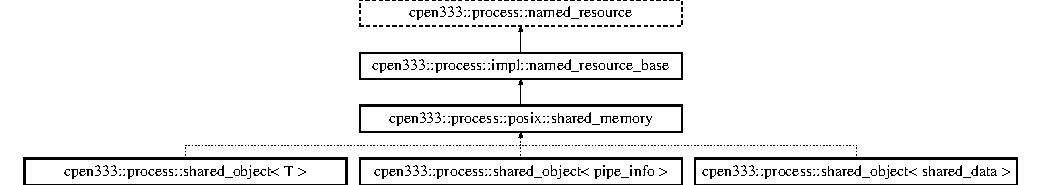
\includegraphics[height=2.488889cm]{classcpen333_1_1process_1_1posix_1_1shared__memory}
\end{center}
\end{figure}
\subsection*{Public Types}
\begin{DoxyCompactItemize}
\item 
\mbox{\Hypertarget{classcpen333_1_1process_1_1posix_1_1shared__memory_a4bec0d0093c8bcfa3283a5da8ef1fc78}\label{classcpen333_1_1process_1_1posix_1_1shared__memory_a4bec0d0093c8bcfa3283a5da8ef1fc78}} 
using \hyperlink{classcpen333_1_1process_1_1posix_1_1shared__memory_a4bec0d0093c8bcfa3283a5da8ef1fc78}{native\+\_\+handle\+\_\+type} = int
\begin{DoxyCompactList}\small\item\em Alias to native handle for shared memory. \end{DoxyCompactList}\end{DoxyCompactItemize}
\subsection*{Public Member Functions}
\begin{DoxyCompactItemize}
\item 
\hyperlink{classcpen333_1_1process_1_1posix_1_1shared__memory_a8a8f0918f8e132e0369c6e9ca9aa6bb6}{shared\+\_\+memory} (const std\+::string \&\hyperlink{classcpen333_1_1process_1_1impl_1_1named__resource__base_ae0c5fbb1843afe863cece4b51c38f807}{name}, size\+\_\+t size, bool readonly=false)
\begin{DoxyCompactList}\small\item\em Constructs or connects to a block of shared memory. \end{DoxyCompactList}\item 
\mbox{\Hypertarget{classcpen333_1_1process_1_1posix_1_1shared__memory_a618389d509320111d7aef051fbd32c07}\label{classcpen333_1_1process_1_1posix_1_1shared__memory_a618389d509320111d7aef051fbd32c07}} 
\hyperlink{classcpen333_1_1process_1_1posix_1_1shared__memory_a618389d509320111d7aef051fbd32c07}{$\sim$shared\+\_\+memory} ()
\begin{DoxyCompactList}\small\item\em Destructor, unmaps this instance of the shared memory block (but does not unmap memory from other users) \end{DoxyCompactList}\item 
bool \hyperlink{classcpen333_1_1process_1_1posix_1_1shared__memory_a3b6d67a41cfaca3712d87958682d8bbe}{unlink} ()
\begin{DoxyCompactList}\small\item\em Detaches the name from the named resource. \end{DoxyCompactList}\item 
void $\ast$ \hyperlink{classcpen333_1_1process_1_1posix_1_1shared__memory_a0611e0aaf945ef86c803bb7907a99f98}{operator-\/$>$} ()
\begin{DoxyCompactList}\small\item\em Pointer operator for accessing underlying data. \end{DoxyCompactList}\item 
void $\ast$ \hyperlink{classcpen333_1_1process_1_1posix_1_1shared__memory_ae97ceec75dc83d43a995daac4769504d}{get} (size\+\_\+t offset=0)
\begin{DoxyCompactList}\small\item\em Pointer to memory at a particular offset from the block. \end{DoxyCompactList}\item 
uint8\+\_\+t \& \hyperlink{classcpen333_1_1process_1_1posix_1_1shared__memory_a832b82cb6ab398e814418b516dba2dd9}{operator\mbox{[}$\,$\mbox{]}} (size\+\_\+t offset)
\begin{DoxyCompactList}\small\item\em Byte access, by reference. \end{DoxyCompactList}\item 
{\footnotesize template$<$typename T $>$ }\\T $\ast$ \hyperlink{classcpen333_1_1process_1_1posix_1_1shared__memory_a09582d7b2863aebbbd74d2f32d0b1af8}{get} (size\+\_\+t offset)
\begin{DoxyCompactList}\small\item\em Retrieves a pointer to an object of specified type starting at a particular offset. \end{DoxyCompactList}\item 
{\footnotesize template$<$typename T $>$ }\\T $\ast$ \hyperlink{classcpen333_1_1process_1_1posix_1_1shared__memory_a705beedc2e0b3bde2e044fe742f641ea}{get} ()
\begin{DoxyCompactList}\small\item\em Retrieves a pointer to the underlying memory, cast to a specified type. \end{DoxyCompactList}\item 
\hyperlink{classcpen333_1_1process_1_1posix_1_1shared__memory_a4bec0d0093c8bcfa3283a5da8ef1fc78}{native\+\_\+handle\+\_\+type} \hyperlink{classcpen333_1_1process_1_1posix_1_1shared__memory_ac0dd258666565953b8c6bdbde7aa871f}{native\+\_\+handle} ()
\begin{DoxyCompactList}\small\item\em Native handle to underlying shared memory block. \end{DoxyCompactList}\end{DoxyCompactItemize}
\subsection*{Static Public Member Functions}
\begin{DoxyCompactItemize}
\item 
static bool \hyperlink{classcpen333_1_1process_1_1posix_1_1shared__memory_a68a9ecfafed3c939bc9c38edee71d584}{unlink} (const std\+::string \&\hyperlink{classcpen333_1_1process_1_1impl_1_1named__resource__base_ae0c5fbb1843afe863cece4b51c38f807}{name})
\begin{DoxyCompactList}\small\item\em Unlinks the name without needing to create a resource. \end{DoxyCompactList}\end{DoxyCompactItemize}
\subsection*{Additional Inherited Members}


\subsection{Detailed Description}
Inter-\/process shared memory implementation. 

Creates and shares a block of memory between threads/processes, accessible using a unique name. The block of memory is mapped to D\+I\+F\+F\+E\+R\+E\+NT address spaces on each process. This is essentially a memory-\/mapped file.

This shared memory has K\+E\+R\+N\+EL P\+E\+R\+S\+I\+S\+T\+E\+N\+CE, meaning if not \hyperlink{classcpen333_1_1process_1_1posix_1_1shared__memory_a3b6d67a41cfaca3712d87958682d8bbe}{unlink()}-\/ed, will continue to exist in its current state until the system is shut down (persisting beyond the life of the initiating program) 

\subsection{Constructor \& Destructor Documentation}
\mbox{\Hypertarget{classcpen333_1_1process_1_1posix_1_1shared__memory_a8a8f0918f8e132e0369c6e9ca9aa6bb6}\label{classcpen333_1_1process_1_1posix_1_1shared__memory_a8a8f0918f8e132e0369c6e9ca9aa6bb6}} 
\index{cpen333\+::process\+::posix\+::shared\+\_\+memory@{cpen333\+::process\+::posix\+::shared\+\_\+memory}!shared\+\_\+memory@{shared\+\_\+memory}}
\index{shared\+\_\+memory@{shared\+\_\+memory}!cpen333\+::process\+::posix\+::shared\+\_\+memory@{cpen333\+::process\+::posix\+::shared\+\_\+memory}}
\subsubsection{\texorpdfstring{shared\+\_\+memory()}{shared\_memory()}}
{\footnotesize\ttfamily cpen333\+::process\+::posix\+::shared\+\_\+memory\+::shared\+\_\+memory (\begin{DoxyParamCaption}\item[{const std\+::string \&}]{name,  }\item[{size\+\_\+t}]{size,  }\item[{bool}]{readonly = {\ttfamily false} }\end{DoxyParamCaption})\hspace{0.3cm}{\ttfamily [inline]}}



Constructs or connects to a block of shared memory. 


\begin{DoxyParams}{Parameters}
{\em name} & identifier for creating or connecting to an existing inter-\/process shared memory block \\
\hline
{\em size} & if creating, the size of the memory block. This size should be consistent between users \\
\hline
{\em readonly} & whether or not to map the memory as read-\/only \\
\hline
\end{DoxyParams}


\subsection{Member Function Documentation}
\mbox{\Hypertarget{classcpen333_1_1process_1_1posix_1_1shared__memory_ae97ceec75dc83d43a995daac4769504d}\label{classcpen333_1_1process_1_1posix_1_1shared__memory_ae97ceec75dc83d43a995daac4769504d}} 
\index{cpen333\+::process\+::posix\+::shared\+\_\+memory@{cpen333\+::process\+::posix\+::shared\+\_\+memory}!get@{get}}
\index{get@{get}!cpen333\+::process\+::posix\+::shared\+\_\+memory@{cpen333\+::process\+::posix\+::shared\+\_\+memory}}
\subsubsection{\texorpdfstring{get()}{get()}\hspace{0.1cm}{\footnotesize\ttfamily [1/3]}}
{\footnotesize\ttfamily void$\ast$ cpen333\+::process\+::posix\+::shared\+\_\+memory\+::get (\begin{DoxyParamCaption}\item[{size\+\_\+t}]{offset = {\ttfamily 0} }\end{DoxyParamCaption})\hspace{0.3cm}{\ttfamily [inline]}}



Pointer to memory at a particular offset from the block. 


\begin{DoxyParams}{Parameters}
{\em offset} & memory offset (in bytes) \\
\hline
\end{DoxyParams}
\begin{DoxyReturn}{Returns}
pointer to memory offset 
\end{DoxyReturn}
\mbox{\Hypertarget{classcpen333_1_1process_1_1posix_1_1shared__memory_a09582d7b2863aebbbd74d2f32d0b1af8}\label{classcpen333_1_1process_1_1posix_1_1shared__memory_a09582d7b2863aebbbd74d2f32d0b1af8}} 
\index{cpen333\+::process\+::posix\+::shared\+\_\+memory@{cpen333\+::process\+::posix\+::shared\+\_\+memory}!get@{get}}
\index{get@{get}!cpen333\+::process\+::posix\+::shared\+\_\+memory@{cpen333\+::process\+::posix\+::shared\+\_\+memory}}
\subsubsection{\texorpdfstring{get()}{get()}\hspace{0.1cm}{\footnotesize\ttfamily [2/3]}}
{\footnotesize\ttfamily template$<$typename T $>$ \\
T$\ast$ cpen333\+::process\+::posix\+::shared\+\_\+memory\+::get (\begin{DoxyParamCaption}\item[{size\+\_\+t}]{offset }\end{DoxyParamCaption})\hspace{0.3cm}{\ttfamily [inline]}}



Retrieves a pointer to an object of specified type starting at a particular offset. 


\begin{DoxyTemplParams}{Template Parameters}
{\em T} & type of pointer to return \\
\hline
\end{DoxyTemplParams}

\begin{DoxyParams}{Parameters}
{\em offset} & memory offset (in bytes) \\
\hline
\end{DoxyParams}
\begin{DoxyReturn}{Returns}
pointer to object 
\end{DoxyReturn}
\mbox{\Hypertarget{classcpen333_1_1process_1_1posix_1_1shared__memory_a705beedc2e0b3bde2e044fe742f641ea}\label{classcpen333_1_1process_1_1posix_1_1shared__memory_a705beedc2e0b3bde2e044fe742f641ea}} 
\index{cpen333\+::process\+::posix\+::shared\+\_\+memory@{cpen333\+::process\+::posix\+::shared\+\_\+memory}!get@{get}}
\index{get@{get}!cpen333\+::process\+::posix\+::shared\+\_\+memory@{cpen333\+::process\+::posix\+::shared\+\_\+memory}}
\subsubsection{\texorpdfstring{get()}{get()}\hspace{0.1cm}{\footnotesize\ttfamily [3/3]}}
{\footnotesize\ttfamily template$<$typename T $>$ \\
T$\ast$ cpen333\+::process\+::posix\+::shared\+\_\+memory\+::get (\begin{DoxyParamCaption}{ }\end{DoxyParamCaption})\hspace{0.3cm}{\ttfamily [inline]}}



Retrieves a pointer to the underlying memory, cast to a specified type. 


\begin{DoxyTemplParams}{Template Parameters}
{\em T} & type of pointer to return \\
\hline
\end{DoxyTemplParams}
\begin{DoxyReturn}{Returns}
pointer to object 
\end{DoxyReturn}
\mbox{\Hypertarget{classcpen333_1_1process_1_1posix_1_1shared__memory_ac0dd258666565953b8c6bdbde7aa871f}\label{classcpen333_1_1process_1_1posix_1_1shared__memory_ac0dd258666565953b8c6bdbde7aa871f}} 
\index{cpen333\+::process\+::posix\+::shared\+\_\+memory@{cpen333\+::process\+::posix\+::shared\+\_\+memory}!native\+\_\+handle@{native\+\_\+handle}}
\index{native\+\_\+handle@{native\+\_\+handle}!cpen333\+::process\+::posix\+::shared\+\_\+memory@{cpen333\+::process\+::posix\+::shared\+\_\+memory}}
\subsubsection{\texorpdfstring{native\+\_\+handle()}{native\_handle()}}
{\footnotesize\ttfamily \hyperlink{classcpen333_1_1process_1_1posix_1_1shared__memory_a4bec0d0093c8bcfa3283a5da8ef1fc78}{native\+\_\+handle\+\_\+type} cpen333\+::process\+::posix\+::shared\+\_\+memory\+::native\+\_\+handle (\begin{DoxyParamCaption}{ }\end{DoxyParamCaption})\hspace{0.3cm}{\ttfamily [inline]}}



Native handle to underlying shared memory block. 

On P\+O\+S\+IX systems, this is a P\+O\+S\+IX shm id

\begin{DoxyReturn}{Returns}
native handle to shared memory block 
\end{DoxyReturn}
\mbox{\Hypertarget{classcpen333_1_1process_1_1posix_1_1shared__memory_a0611e0aaf945ef86c803bb7907a99f98}\label{classcpen333_1_1process_1_1posix_1_1shared__memory_a0611e0aaf945ef86c803bb7907a99f98}} 
\index{cpen333\+::process\+::posix\+::shared\+\_\+memory@{cpen333\+::process\+::posix\+::shared\+\_\+memory}!operator-\/$>$@{operator-\/$>$}}
\index{operator-\/$>$@{operator-\/$>$}!cpen333\+::process\+::posix\+::shared\+\_\+memory@{cpen333\+::process\+::posix\+::shared\+\_\+memory}}
\subsubsection{\texorpdfstring{operator-\/$>$()}{operator->()}}
{\footnotesize\ttfamily void$\ast$ cpen333\+::process\+::posix\+::shared\+\_\+memory\+::operator-\/$>$ (\begin{DoxyParamCaption}{ }\end{DoxyParamCaption})\hspace{0.3cm}{\ttfamily [inline]}}



Pointer operator for accessing underlying data. 

\begin{DoxyReturn}{Returns}
pointer to underlying data 
\end{DoxyReturn}
\mbox{\Hypertarget{classcpen333_1_1process_1_1posix_1_1shared__memory_a832b82cb6ab398e814418b516dba2dd9}\label{classcpen333_1_1process_1_1posix_1_1shared__memory_a832b82cb6ab398e814418b516dba2dd9}} 
\index{cpen333\+::process\+::posix\+::shared\+\_\+memory@{cpen333\+::process\+::posix\+::shared\+\_\+memory}!operator\mbox{[}\mbox{]}@{operator[]}}
\index{operator\mbox{[}\mbox{]}@{operator[]}!cpen333\+::process\+::posix\+::shared\+\_\+memory@{cpen333\+::process\+::posix\+::shared\+\_\+memory}}
\subsubsection{\texorpdfstring{operator[]()}{operator[]()}}
{\footnotesize\ttfamily uint8\+\_\+t\& cpen333\+::process\+::posix\+::shared\+\_\+memory\+::operator\mbox{[}$\,$\mbox{]} (\begin{DoxyParamCaption}\item[{size\+\_\+t}]{offset }\end{DoxyParamCaption})\hspace{0.3cm}{\ttfamily [inline]}}



Byte access, by reference. 


\begin{DoxyParams}{Parameters}
{\em offset} & memory offset (in bytes) \\
\hline
\end{DoxyParams}
\begin{DoxyReturn}{Returns}
byte at particular offset 
\end{DoxyReturn}
\mbox{\Hypertarget{classcpen333_1_1process_1_1posix_1_1shared__memory_a3b6d67a41cfaca3712d87958682d8bbe}\label{classcpen333_1_1process_1_1posix_1_1shared__memory_a3b6d67a41cfaca3712d87958682d8bbe}} 
\index{cpen333\+::process\+::posix\+::shared\+\_\+memory@{cpen333\+::process\+::posix\+::shared\+\_\+memory}!unlink@{unlink}}
\index{unlink@{unlink}!cpen333\+::process\+::posix\+::shared\+\_\+memory@{cpen333\+::process\+::posix\+::shared\+\_\+memory}}
\subsubsection{\texorpdfstring{unlink()}{unlink()}\hspace{0.1cm}{\footnotesize\ttfamily [1/2]}}
{\footnotesize\ttfamily bool cpen333\+::process\+::posix\+::shared\+\_\+memory\+::unlink (\begin{DoxyParamCaption}{ }\end{DoxyParamCaption})\hspace{0.3cm}{\ttfamily [inline]}, {\ttfamily [virtual]}}



Detaches the name from the named resource. 

On P\+O\+S\+IX systems, named resources will persist beyond the lifetime of any process that uses them as long as the name has not been unlinked (or until the system is rebooted). Calling {\ttfamily unlink} will detach the name, allowing the resource to be freed once all current users have exited.

\begin{DoxyReturn}{Returns}
{\ttfamily true} if unlink is successful, {\ttfamily false} if unlinking is not supported or if an error has occurred. 
\end{DoxyReturn}


Implements \hyperlink{classcpen333_1_1process_1_1impl_1_1named__resource__base_ae4033f82dfd068b917a9bca57d3a0c45}{cpen333\+::process\+::impl\+::named\+\_\+resource\+\_\+base}.



Reimplemented in \hyperlink{classcpen333_1_1process_1_1shared__object_aa5b43829da5bd2376927e6285745211c}{cpen333\+::process\+::shared\+\_\+object$<$ T $>$}, \hyperlink{classcpen333_1_1process_1_1shared__object_aa5b43829da5bd2376927e6285745211c}{cpen333\+::process\+::shared\+\_\+object$<$ pipe\+\_\+info $>$}, and \hyperlink{classcpen333_1_1process_1_1shared__object_aa5b43829da5bd2376927e6285745211c}{cpen333\+::process\+::shared\+\_\+object$<$ shared\+\_\+data $>$}.

\mbox{\Hypertarget{classcpen333_1_1process_1_1posix_1_1shared__memory_a68a9ecfafed3c939bc9c38edee71d584}\label{classcpen333_1_1process_1_1posix_1_1shared__memory_a68a9ecfafed3c939bc9c38edee71d584}} 
\index{cpen333\+::process\+::posix\+::shared\+\_\+memory@{cpen333\+::process\+::posix\+::shared\+\_\+memory}!unlink@{unlink}}
\index{unlink@{unlink}!cpen333\+::process\+::posix\+::shared\+\_\+memory@{cpen333\+::process\+::posix\+::shared\+\_\+memory}}
\subsubsection{\texorpdfstring{unlink()}{unlink()}\hspace{0.1cm}{\footnotesize\ttfamily [2/2]}}
{\footnotesize\ttfamily static bool cpen333\+::process\+::posix\+::shared\+\_\+memory\+::unlink (\begin{DoxyParamCaption}\item[{const std\+::string \&}]{name }\end{DoxyParamCaption})\hspace{0.3cm}{\ttfamily [inline]}, {\ttfamily [static]}}



Unlinks the name without needing to create a resource. 

Implementers should also provide a static method for unlinking. The purpose is mainly for clean-\/up of existing resources.


\begin{DoxyParams}{Parameters}
{\em name} & desired resource name \\
\hline
\end{DoxyParams}
\begin{DoxyReturn}{Returns}
{\ttfamily true} if unlink successful, {\ttfamily false} if not successful or not supported 
\end{DoxyReturn}


The documentation for this class was generated from the following file\+:\begin{DoxyCompactItemize}
\item 
D\+:/school/teaching/\+C\+P\+E\+N333/workspace/library/include/cpen333/process/impl/posix/\hyperlink{impl_2posix_2shared__memory_8h}{shared\+\_\+memory.\+h}\end{DoxyCompactItemize}

\hypertarget{classcpen333_1_1process_1_1windows_1_1shared__memory}{}\section{cpen333\+:\+:process\+:\+:windows\+:\+:shared\+\_\+memory Class Reference}
\label{classcpen333_1_1process_1_1windows_1_1shared__memory}\index{cpen333\+::process\+::windows\+::shared\+\_\+memory@{cpen333\+::process\+::windows\+::shared\+\_\+memory}}


Inter-\/process shared memory implementation.  




{\ttfamily \#include $<$shared\+\_\+memory.\+h$>$}

Inheritance diagram for cpen333\+:\+:process\+:\+:windows\+:\+:shared\+\_\+memory\+:\begin{figure}[H]
\begin{center}
\leavevmode
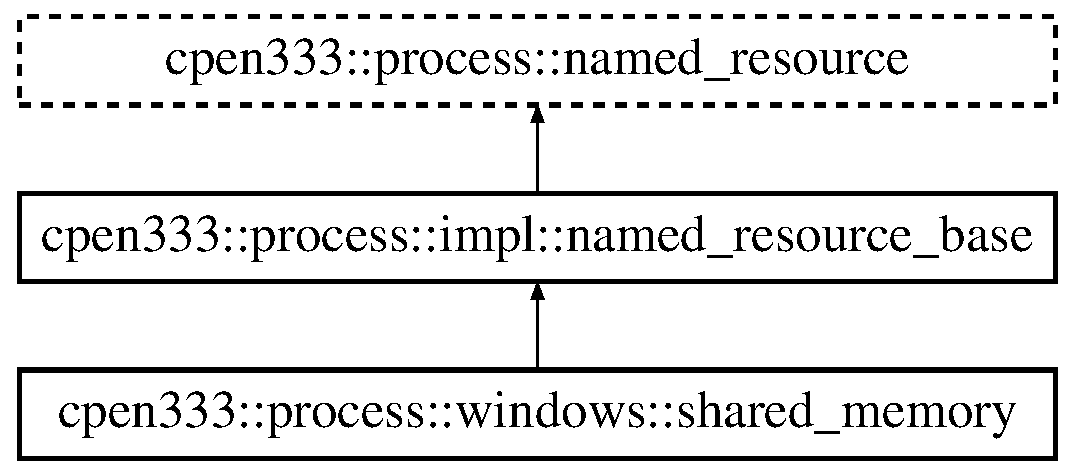
\includegraphics[height=3.000000cm]{classcpen333_1_1process_1_1windows_1_1shared__memory}
\end{center}
\end{figure}
\subsection*{Public Types}
\begin{DoxyCompactItemize}
\item 
\mbox{\Hypertarget{classcpen333_1_1process_1_1windows_1_1shared__memory_a92d977097375f7b87d5702b7da666267}\label{classcpen333_1_1process_1_1windows_1_1shared__memory_a92d977097375f7b87d5702b7da666267}} 
using \hyperlink{classcpen333_1_1process_1_1windows_1_1shared__memory_a92d977097375f7b87d5702b7da666267}{native\+\_\+handle\+\_\+type} = H\+A\+N\+D\+LE
\begin{DoxyCompactList}\small\item\em Alias to native handle for shared memory. \end{DoxyCompactList}\end{DoxyCompactItemize}
\subsection*{Public Member Functions}
\begin{DoxyCompactItemize}
\item 
\hyperlink{classcpen333_1_1process_1_1windows_1_1shared__memory_a3a2044ba961f9fc394e166273a3efa20}{shared\+\_\+memory} (const std\+::string \&\hyperlink{classcpen333_1_1process_1_1impl_1_1named__resource__base_ae0c5fbb1843afe863cece4b51c38f807}{name}, size\+\_\+t size, bool readonly=false)
\begin{DoxyCompactList}\small\item\em Constructs or connects to a block of shared memory. \end{DoxyCompactList}\item 
\hyperlink{classcpen333_1_1process_1_1windows_1_1shared__memory_a6355690147ae22f25d4bceed8ad63011}{$\sim$shared\+\_\+memory} ()
\begin{DoxyCompactList}\small\item\em Destructor, unmaps this instance of the shared memory block (but does not unmap memory from other users) \end{DoxyCompactList}\item 
void $\ast$ \hyperlink{classcpen333_1_1process_1_1windows_1_1shared__memory_a2afcb6ba09ba1039c2e03efb471d3b28}{operator-\/$>$} ()
\begin{DoxyCompactList}\small\item\em Pointer operator for accessing underlying data. \end{DoxyCompactList}\item 
void $\ast$ \hyperlink{classcpen333_1_1process_1_1windows_1_1shared__memory_a3bbd718728dc2fa2fbe4058b8a207594}{get} (size\+\_\+t offset=0)
\begin{DoxyCompactList}\small\item\em Pointer to memory at a particular offset from the block. \end{DoxyCompactList}\item 
uint8\+\_\+t \& \hyperlink{classcpen333_1_1process_1_1windows_1_1shared__memory_a931719bdcc1558973d6fcb7a79f52f22}{operator\mbox{[}$\,$\mbox{]}} (size\+\_\+t offset)
\begin{DoxyCompactList}\small\item\em Byte access, by reference. \end{DoxyCompactList}\item 
{\footnotesize template$<$typename T $>$ }\\T $\ast$ \hyperlink{classcpen333_1_1process_1_1windows_1_1shared__memory_a2f2fa53c705df531b6126ed2da84c347}{get} (size\+\_\+t offset)
\begin{DoxyCompactList}\small\item\em Pointer to memory at a particular offset from the block. \end{DoxyCompactList}\item 
{\footnotesize template$<$typename T $>$ }\\T $\ast$ \hyperlink{classcpen333_1_1process_1_1windows_1_1shared__memory_a3986cdc917b26ab1ab608f59270a47c5}{get} ()
\begin{DoxyCompactList}\small\item\em Retrieves a pointer to the underlying memory, cast to a specified type. \end{DoxyCompactList}\item 
\hyperlink{classcpen333_1_1process_1_1windows_1_1shared__memory_a92d977097375f7b87d5702b7da666267}{native\+\_\+handle\+\_\+type} \hyperlink{classcpen333_1_1process_1_1windows_1_1shared__memory_a1827dd03341d7c6afcc02cf078f54e32}{native\+\_\+handle} ()
\begin{DoxyCompactList}\small\item\em Native handle to underlying shared memory block. \end{DoxyCompactList}\item 
bool \hyperlink{classcpen333_1_1process_1_1windows_1_1shared__memory_aa6efdc9a3e1310ea69ecc48aeb41286c}{unlink} ()
\begin{DoxyCompactList}\small\item\em Detaches the name from the named resource. \end{DoxyCompactList}\end{DoxyCompactItemize}
\subsection*{Static Public Member Functions}
\begin{DoxyCompactItemize}
\item 
static bool \hyperlink{classcpen333_1_1process_1_1windows_1_1shared__memory_a99c4766a9995a97595bba1550256f1c9}{unlink} (const std\+::string \&\hyperlink{classcpen333_1_1process_1_1impl_1_1named__resource__base_ae0c5fbb1843afe863cece4b51c38f807}{name})
\begin{DoxyCompactList}\small\item\em Unlinks the name without needing to create a resource. \end{DoxyCompactList}\end{DoxyCompactItemize}
\subsection*{Additional Inherited Members}


\subsection{Detailed Description}
Inter-\/process shared memory implementation. 

Creates and shares a block of memory between threads/processes, accessible using a unique name. The block of memory is mapped to D\+I\+F\+F\+E\+R\+E\+NT address spaces on each process. This is essentially a memory-\/mapped file.

This shared memory has U\+S\+A\+GE P\+E\+R\+S\+I\+S\+T\+E\+N\+CE, meaning the mutex will continue to exist as long as at least one process/thread is holding a reference to it. 

\subsection{Constructor \& Destructor Documentation}
\mbox{\Hypertarget{classcpen333_1_1process_1_1windows_1_1shared__memory_a3a2044ba961f9fc394e166273a3efa20}\label{classcpen333_1_1process_1_1windows_1_1shared__memory_a3a2044ba961f9fc394e166273a3efa20}} 
\index{cpen333\+::process\+::windows\+::shared\+\_\+memory@{cpen333\+::process\+::windows\+::shared\+\_\+memory}!shared\+\_\+memory@{shared\+\_\+memory}}
\index{shared\+\_\+memory@{shared\+\_\+memory}!cpen333\+::process\+::windows\+::shared\+\_\+memory@{cpen333\+::process\+::windows\+::shared\+\_\+memory}}
\subsubsection{\texorpdfstring{shared\+\_\+memory()}{shared\_memory()}}
{\footnotesize\ttfamily cpen333\+::process\+::windows\+::shared\+\_\+memory\+::shared\+\_\+memory (\begin{DoxyParamCaption}\item[{const std\+::string \&}]{name,  }\item[{size\+\_\+t}]{size,  }\item[{bool}]{readonly = {\ttfamily false} }\end{DoxyParamCaption})\hspace{0.3cm}{\ttfamily [inline]}}



Constructs or connects to a block of shared memory. 


\begin{DoxyParams}{Parameters}
{\em name} & identifier for creating or connecting to an existing inter-\/process shared memory block \\
\hline
{\em size} & if creating, the size of the memory block. This size should be consistent between users \\
\hline
{\em readonly} & whether or not to map the memory as read-\/only \\
\hline
\end{DoxyParams}
\mbox{\Hypertarget{classcpen333_1_1process_1_1windows_1_1shared__memory_a6355690147ae22f25d4bceed8ad63011}\label{classcpen333_1_1process_1_1windows_1_1shared__memory_a6355690147ae22f25d4bceed8ad63011}} 
\index{cpen333\+::process\+::windows\+::shared\+\_\+memory@{cpen333\+::process\+::windows\+::shared\+\_\+memory}!````~shared\+\_\+memory@{$\sim$shared\+\_\+memory}}
\index{````~shared\+\_\+memory@{$\sim$shared\+\_\+memory}!cpen333\+::process\+::windows\+::shared\+\_\+memory@{cpen333\+::process\+::windows\+::shared\+\_\+memory}}
\subsubsection{\texorpdfstring{$\sim$shared\+\_\+memory()}{~shared\_memory()}}
{\footnotesize\ttfamily cpen333\+::process\+::windows\+::shared\+\_\+memory\+::$\sim$shared\+\_\+memory (\begin{DoxyParamCaption}{ }\end{DoxyParamCaption})\hspace{0.3cm}{\ttfamily [inline]}}



Destructor, unmaps this instance of the shared memory block (but does not unmap memory from other users) 



\subsection{Member Function Documentation}
\mbox{\Hypertarget{classcpen333_1_1process_1_1windows_1_1shared__memory_a3bbd718728dc2fa2fbe4058b8a207594}\label{classcpen333_1_1process_1_1windows_1_1shared__memory_a3bbd718728dc2fa2fbe4058b8a207594}} 
\index{cpen333\+::process\+::windows\+::shared\+\_\+memory@{cpen333\+::process\+::windows\+::shared\+\_\+memory}!get@{get}}
\index{get@{get}!cpen333\+::process\+::windows\+::shared\+\_\+memory@{cpen333\+::process\+::windows\+::shared\+\_\+memory}}
\subsubsection{\texorpdfstring{get()}{get()}\hspace{0.1cm}{\footnotesize\ttfamily [1/3]}}
{\footnotesize\ttfamily void$\ast$ cpen333\+::process\+::windows\+::shared\+\_\+memory\+::get (\begin{DoxyParamCaption}\item[{size\+\_\+t}]{offset = {\ttfamily 0} }\end{DoxyParamCaption})\hspace{0.3cm}{\ttfamily [inline]}}



Pointer to memory at a particular offset from the block. 


\begin{DoxyParams}{Parameters}
{\em offset} & memory offset (in bytes) \\
\hline
\end{DoxyParams}
\begin{DoxyReturn}{Returns}
pointer to memory offset 
\end{DoxyReturn}
\mbox{\Hypertarget{classcpen333_1_1process_1_1windows_1_1shared__memory_a2f2fa53c705df531b6126ed2da84c347}\label{classcpen333_1_1process_1_1windows_1_1shared__memory_a2f2fa53c705df531b6126ed2da84c347}} 
\index{cpen333\+::process\+::windows\+::shared\+\_\+memory@{cpen333\+::process\+::windows\+::shared\+\_\+memory}!get@{get}}
\index{get@{get}!cpen333\+::process\+::windows\+::shared\+\_\+memory@{cpen333\+::process\+::windows\+::shared\+\_\+memory}}
\subsubsection{\texorpdfstring{get()}{get()}\hspace{0.1cm}{\footnotesize\ttfamily [2/3]}}
{\footnotesize\ttfamily template$<$typename T $>$ \\
T$\ast$ cpen333\+::process\+::windows\+::shared\+\_\+memory\+::get (\begin{DoxyParamCaption}\item[{size\+\_\+t}]{offset }\end{DoxyParamCaption})\hspace{0.3cm}{\ttfamily [inline]}}



Pointer to memory at a particular offset from the block. 


\begin{DoxyParams}{Parameters}
{\em offset} & memory offset (in bytes) \\
\hline
\end{DoxyParams}
\begin{DoxyReturn}{Returns}
pointer to memory offset 
\end{DoxyReturn}
\mbox{\Hypertarget{classcpen333_1_1process_1_1windows_1_1shared__memory_a3986cdc917b26ab1ab608f59270a47c5}\label{classcpen333_1_1process_1_1windows_1_1shared__memory_a3986cdc917b26ab1ab608f59270a47c5}} 
\index{cpen333\+::process\+::windows\+::shared\+\_\+memory@{cpen333\+::process\+::windows\+::shared\+\_\+memory}!get@{get}}
\index{get@{get}!cpen333\+::process\+::windows\+::shared\+\_\+memory@{cpen333\+::process\+::windows\+::shared\+\_\+memory}}
\subsubsection{\texorpdfstring{get()}{get()}\hspace{0.1cm}{\footnotesize\ttfamily [3/3]}}
{\footnotesize\ttfamily template$<$typename T $>$ \\
T$\ast$ cpen333\+::process\+::windows\+::shared\+\_\+memory\+::get (\begin{DoxyParamCaption}{ }\end{DoxyParamCaption})\hspace{0.3cm}{\ttfamily [inline]}}



Retrieves a pointer to the underlying memory, cast to a specified type. 


\begin{DoxyTemplParams}{Template Parameters}
{\em T} & type of pointer to return \\
\hline
\end{DoxyTemplParams}
\begin{DoxyReturn}{Returns}
pointer to object 
\end{DoxyReturn}
\mbox{\Hypertarget{classcpen333_1_1process_1_1windows_1_1shared__memory_a1827dd03341d7c6afcc02cf078f54e32}\label{classcpen333_1_1process_1_1windows_1_1shared__memory_a1827dd03341d7c6afcc02cf078f54e32}} 
\index{cpen333\+::process\+::windows\+::shared\+\_\+memory@{cpen333\+::process\+::windows\+::shared\+\_\+memory}!native\+\_\+handle@{native\+\_\+handle}}
\index{native\+\_\+handle@{native\+\_\+handle}!cpen333\+::process\+::windows\+::shared\+\_\+memory@{cpen333\+::process\+::windows\+::shared\+\_\+memory}}
\subsubsection{\texorpdfstring{native\+\_\+handle()}{native\_handle()}}
{\footnotesize\ttfamily \hyperlink{classcpen333_1_1process_1_1windows_1_1shared__memory_a92d977097375f7b87d5702b7da666267}{native\+\_\+handle\+\_\+type} cpen333\+::process\+::windows\+::shared\+\_\+memory\+::native\+\_\+handle (\begin{DoxyParamCaption}{ }\end{DoxyParamCaption})\hspace{0.3cm}{\ttfamily [inline]}}



Native handle to underlying shared memory block. 

On Windows systems, this is a Windows H\+A\+N\+D\+LE to the memory-\/mapped file mapping

\begin{DoxyReturn}{Returns}
native handle to shared memory block 
\end{DoxyReturn}
\mbox{\Hypertarget{classcpen333_1_1process_1_1windows_1_1shared__memory_a2afcb6ba09ba1039c2e03efb471d3b28}\label{classcpen333_1_1process_1_1windows_1_1shared__memory_a2afcb6ba09ba1039c2e03efb471d3b28}} 
\index{cpen333\+::process\+::windows\+::shared\+\_\+memory@{cpen333\+::process\+::windows\+::shared\+\_\+memory}!operator-\/$>$@{operator-\/$>$}}
\index{operator-\/$>$@{operator-\/$>$}!cpen333\+::process\+::windows\+::shared\+\_\+memory@{cpen333\+::process\+::windows\+::shared\+\_\+memory}}
\subsubsection{\texorpdfstring{operator-\/$>$()}{operator->()}}
{\footnotesize\ttfamily void$\ast$ cpen333\+::process\+::windows\+::shared\+\_\+memory\+::operator-\/$>$ (\begin{DoxyParamCaption}{ }\end{DoxyParamCaption})\hspace{0.3cm}{\ttfamily [inline]}}



Pointer operator for accessing underlying data. 

\begin{DoxyReturn}{Returns}
pointer to underlying data 
\end{DoxyReturn}
\mbox{\Hypertarget{classcpen333_1_1process_1_1windows_1_1shared__memory_a931719bdcc1558973d6fcb7a79f52f22}\label{classcpen333_1_1process_1_1windows_1_1shared__memory_a931719bdcc1558973d6fcb7a79f52f22}} 
\index{cpen333\+::process\+::windows\+::shared\+\_\+memory@{cpen333\+::process\+::windows\+::shared\+\_\+memory}!operator\mbox{[}\mbox{]}@{operator[]}}
\index{operator\mbox{[}\mbox{]}@{operator[]}!cpen333\+::process\+::windows\+::shared\+\_\+memory@{cpen333\+::process\+::windows\+::shared\+\_\+memory}}
\subsubsection{\texorpdfstring{operator[]()}{operator[]()}}
{\footnotesize\ttfamily uint8\+\_\+t\& cpen333\+::process\+::windows\+::shared\+\_\+memory\+::operator\mbox{[}$\,$\mbox{]} (\begin{DoxyParamCaption}\item[{size\+\_\+t}]{offset }\end{DoxyParamCaption})\hspace{0.3cm}{\ttfamily [inline]}}



Byte access, by reference. 


\begin{DoxyParams}{Parameters}
{\em offset} & memory offset (in bytes) \\
\hline
\end{DoxyParams}
\begin{DoxyReturn}{Returns}
byte at particular offset 
\end{DoxyReturn}
\mbox{\Hypertarget{classcpen333_1_1process_1_1windows_1_1shared__memory_aa6efdc9a3e1310ea69ecc48aeb41286c}\label{classcpen333_1_1process_1_1windows_1_1shared__memory_aa6efdc9a3e1310ea69ecc48aeb41286c}} 
\index{cpen333\+::process\+::windows\+::shared\+\_\+memory@{cpen333\+::process\+::windows\+::shared\+\_\+memory}!unlink@{unlink}}
\index{unlink@{unlink}!cpen333\+::process\+::windows\+::shared\+\_\+memory@{cpen333\+::process\+::windows\+::shared\+\_\+memory}}
\subsubsection{\texorpdfstring{unlink()}{unlink()}\hspace{0.1cm}{\footnotesize\ttfamily [1/2]}}
{\footnotesize\ttfamily bool cpen333\+::process\+::windows\+::shared\+\_\+memory\+::unlink (\begin{DoxyParamCaption}{ }\end{DoxyParamCaption})\hspace{0.3cm}{\ttfamily [inline]}, {\ttfamily [virtual]}}



Detaches the name from the named resource. 

On P\+O\+S\+IX systems, named resources will persist beyond the lifetime of any process that uses them as long as the name has not been unlinked (or until the system is rebooted). Calling {\ttfamily unlink} will detach the name, allowing the resource to be freed once all current users have exited.

\begin{DoxyReturn}{Returns}
{\ttfamily true} if unlink is successful, {\ttfamily false} if unlinking is not supported or if an error has occurred. 
\end{DoxyReturn}


Implements \hyperlink{classcpen333_1_1process_1_1impl_1_1named__resource__base_ae4033f82dfd068b917a9bca57d3a0c45}{cpen333\+::process\+::impl\+::named\+\_\+resource\+\_\+base}.

\mbox{\Hypertarget{classcpen333_1_1process_1_1windows_1_1shared__memory_a99c4766a9995a97595bba1550256f1c9}\label{classcpen333_1_1process_1_1windows_1_1shared__memory_a99c4766a9995a97595bba1550256f1c9}} 
\index{cpen333\+::process\+::windows\+::shared\+\_\+memory@{cpen333\+::process\+::windows\+::shared\+\_\+memory}!unlink@{unlink}}
\index{unlink@{unlink}!cpen333\+::process\+::windows\+::shared\+\_\+memory@{cpen333\+::process\+::windows\+::shared\+\_\+memory}}
\subsubsection{\texorpdfstring{unlink()}{unlink()}\hspace{0.1cm}{\footnotesize\ttfamily [2/2]}}
{\footnotesize\ttfamily static bool cpen333\+::process\+::windows\+::shared\+\_\+memory\+::unlink (\begin{DoxyParamCaption}\item[{const std\+::string \&}]{name }\end{DoxyParamCaption})\hspace{0.3cm}{\ttfamily [inline]}, {\ttfamily [static]}}



Unlinks the name without needing to create a resource. 

Implementers should also provide a static method for unlinking. The purpose is mainly for clean-\/up of existing resources.


\begin{DoxyParams}{Parameters}
{\em name} & desired resource name \\
\hline
\end{DoxyParams}
\begin{DoxyReturn}{Returns}
{\ttfamily true} if unlink successful, {\ttfamily false} if not successful or not supported 
\end{DoxyReturn}


The documentation for this class was generated from the following file\+:\begin{DoxyCompactItemize}
\item 
D\+:/school/teaching/\+C\+P\+E\+N333/workspace/labs/include/cpen333/process/impl/windows/\hyperlink{impl_2windows_2shared__memory_8h}{shared\+\_\+memory.\+h}\end{DoxyCompactItemize}

\hypertarget{classcpen333_1_1process_1_1shared__mutex}{}\section{cpen333\+:\+:process\+:\+:shared\+\_\+mutex Class Reference}
\label{classcpen333_1_1process_1_1shared__mutex}\index{cpen333\+::process\+::shared\+\_\+mutex@{cpen333\+::process\+::shared\+\_\+mutex}}


An inter-\/process mutual exclusion synchronization primitive allowing for shared access.  




{\ttfamily \#include $<$shared\+\_\+mutex.\+h$>$}



\subsection{Detailed Description}
An inter-\/process mutual exclusion synchronization primitive allowing for shared access. 

Used to protect access to a resource shared by multiple processes, allowing shared `read\textquotesingle{} access, mirroring std\+::shared\+\_\+mutex in c++17. This is an alias to \hyperlink{classcpen333_1_1process_1_1impl_1_1shared__mutex__fair}{cpen333\+::process\+::impl\+::shared\+\_\+mutex\+\_\+fair}. 

The documentation for this class was generated from the following file\+:\begin{DoxyCompactItemize}
\item 
D\+:/school/teaching/\+C\+P\+E\+N333/workspace/labs/include/cpen333/process/\hyperlink{process_2shared__mutex_8h}{shared\+\_\+mutex.\+h}\end{DoxyCompactItemize}

\hypertarget{classcpen333_1_1process_1_1impl_1_1shared__mutex__exclusive}{}\section{cpen333\+:\+:process\+:\+:impl\+:\+:shared\+\_\+mutex\+\_\+exclusive Class Reference}
\label{classcpen333_1_1process_1_1impl_1_1shared__mutex__exclusive}\index{cpen333\+::process\+::impl\+::shared\+\_\+mutex\+\_\+exclusive@{cpen333\+::process\+::impl\+::shared\+\_\+mutex\+\_\+exclusive}}


A write-\/preferring inter-\/process shared mutex implementation.  




{\ttfamily \#include $<$shared\+\_\+mutex\+\_\+exclusive.\+h$>$}

Inheritance diagram for cpen333\+:\+:process\+:\+:impl\+:\+:shared\+\_\+mutex\+\_\+exclusive\+:\begin{figure}[H]
\begin{center}
\leavevmode
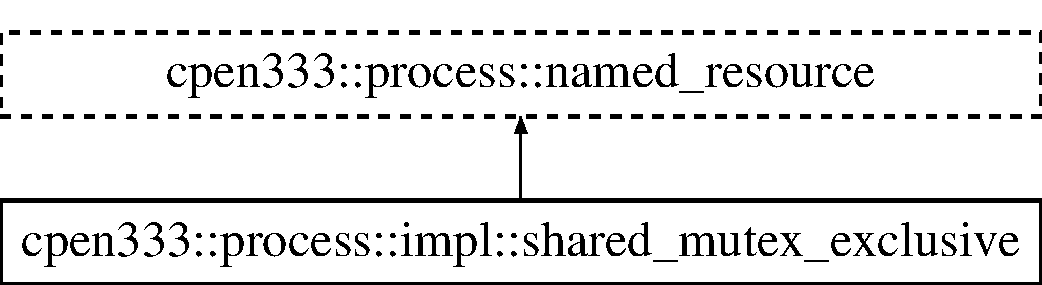
\includegraphics[height=2.000000cm]{classcpen333_1_1process_1_1impl_1_1shared__mutex__exclusive}
\end{center}
\end{figure}
\subsection*{Public Member Functions}
\begin{DoxyCompactItemize}
\item 
\hyperlink{classcpen333_1_1process_1_1impl_1_1shared__mutex__exclusive_a3acb5fa0c2f3f12200d194d53f7dfad4}{shared\+\_\+mutex\+\_\+exclusive} (const std\+::string \&name)
\item 
void \hyperlink{classcpen333_1_1process_1_1impl_1_1shared__mutex__exclusive_ae512adfb383e28ca05d0e1e84f79a898}{lock\+\_\+shared} ()
\begin{DoxyCompactList}\small\item\em Lock the mutex in shared access mode. \end{DoxyCompactList}\item 
bool \hyperlink{classcpen333_1_1process_1_1impl_1_1shared__mutex__exclusive_a0e2e6a0afb83c06d70ceca86e591732f}{try\+\_\+lock\+\_\+shared} ()
\begin{DoxyCompactList}\small\item\em Tries to lock the mutex in shared access mode. \end{DoxyCompactList}\item 
void \hyperlink{classcpen333_1_1process_1_1impl_1_1shared__mutex__exclusive_a01bc4be0f17231c08d8a06f1341acc81}{unlock\+\_\+shared} ()
\begin{DoxyCompactList}\small\item\em Unlocks one instance of shared access. \end{DoxyCompactList}\item 
void \hyperlink{classcpen333_1_1process_1_1impl_1_1shared__mutex__exclusive_a6b6d61dce0f1a536d24e280c4e7ac9a9}{lock} ()
\begin{DoxyCompactList}\small\item\em Locks the mutex in exclusive access mode. \end{DoxyCompactList}\item 
bool \hyperlink{classcpen333_1_1process_1_1impl_1_1shared__mutex__exclusive_aa7b41d55016b38a9d51f23d8c8468857}{try\+\_\+lock} ()
\begin{DoxyCompactList}\small\item\em Tries to lock the mutex in exclusive access mode. \end{DoxyCompactList}\item 
\mbox{\Hypertarget{classcpen333_1_1process_1_1impl_1_1shared__mutex__exclusive_ae7f2d10376f1b1fffe20141ec136a721}\label{classcpen333_1_1process_1_1impl_1_1shared__mutex__exclusive_ae7f2d10376f1b1fffe20141ec136a721}} 
void \hyperlink{classcpen333_1_1process_1_1impl_1_1shared__mutex__exclusive_ae7f2d10376f1b1fffe20141ec136a721}{unlock} ()
\begin{DoxyCompactList}\small\item\em Unlocks the exclusively-\/locked mutex. \end{DoxyCompactList}\item 
{\footnotesize template$<$class Rep , class Period $>$ }\\bool \hyperlink{classcpen333_1_1process_1_1impl_1_1shared__mutex__exclusive_a6f74ff596d66d4ac6b8e7793b8dca78d}{try\+\_\+lock\+\_\+for} (const std\+::chrono\+::duration$<$ Rep, Period $>$ \&timeout\+\_\+duration)
\begin{DoxyCompactList}\small\item\em Try to exclusively lock the mutex, with a relative timeout. \end{DoxyCompactList}\item 
{\footnotesize template$<$class Clock , class Duration $>$ }\\bool \hyperlink{classcpen333_1_1process_1_1impl_1_1shared__mutex__exclusive_ada5717115b6cc1794422c4ae0a691a07}{try\+\_\+lock\+\_\+until} (const std\+::chrono\+::time\+\_\+point$<$ Clock, Duration $>$ \&timeout\+\_\+time)
\begin{DoxyCompactList}\small\item\em Try to exclusively lock the mutex, within an absolute timeout period. \end{DoxyCompactList}\item 
{\footnotesize template$<$class Rep , class Period $>$ }\\bool \hyperlink{classcpen333_1_1process_1_1impl_1_1shared__mutex__exclusive_a655b0bf8c84c6711e2120540d1c77c04}{try\+\_\+lock\+\_\+shared\+\_\+for} (const std\+::chrono\+::duration$<$ Rep, Period $>$ \&timeout\+\_\+duration)
\begin{DoxyCompactList}\small\item\em Try to lock the mutex in shared mode, with a relative timeout. \end{DoxyCompactList}\item 
{\footnotesize template$<$class Clock , class Duration $>$ }\\bool \hyperlink{classcpen333_1_1process_1_1impl_1_1shared__mutex__exclusive_aaf84cb604f6486ab2c627f236753cb7c}{try\+\_\+lock\+\_\+shared\+\_\+until} (const std\+::chrono\+::time\+\_\+point$<$ Clock, Duration $>$ \&timeout\+\_\+time)
\begin{DoxyCompactList}\small\item\em Try to lock the mutex in shared mode, with absolute timeout. \end{DoxyCompactList}\item 
bool \hyperlink{classcpen333_1_1process_1_1impl_1_1shared__mutex__exclusive_ad296e92049cc48cc3c40ec7404bf836c}{unlink} ()
\begin{DoxyCompactList}\small\item\em Detaches the name from the named resource. \end{DoxyCompactList}\end{DoxyCompactItemize}
\subsection*{Static Public Member Functions}
\begin{DoxyCompactItemize}
\item 
static bool \hyperlink{classcpen333_1_1process_1_1impl_1_1shared__mutex__exclusive_a5d16bc8d626096e38d6ca13b23de572e}{unlink} (const std\+::string \&name)
\begin{DoxyCompactList}\small\item\em Unlinks the name without needing to create a resource. \end{DoxyCompactList}\end{DoxyCompactItemize}


\subsection{Detailed Description}
A write-\/preferring inter-\/process shared mutex implementation. 

Inter-\/process shared mutex implementation based on the mutex/semaphore pattern. Gives priority to exclusive access.

See \href{https://en.wikipedia.org/wiki/Readers%E2%80%93writer_lock}{\tt https\+://en.\+wikipedia.\+org/wiki/\+Readers\%\+E2\%80\%93writer\+\_\+lock} for details 

\subsection{Constructor \& Destructor Documentation}
\mbox{\Hypertarget{classcpen333_1_1process_1_1impl_1_1shared__mutex__exclusive_a3acb5fa0c2f3f12200d194d53f7dfad4}\label{classcpen333_1_1process_1_1impl_1_1shared__mutex__exclusive_a3acb5fa0c2f3f12200d194d53f7dfad4}} 
\index{cpen333\+::process\+::impl\+::shared\+\_\+mutex\+\_\+exclusive@{cpen333\+::process\+::impl\+::shared\+\_\+mutex\+\_\+exclusive}!shared\+\_\+mutex\+\_\+exclusive@{shared\+\_\+mutex\+\_\+exclusive}}
\index{shared\+\_\+mutex\+\_\+exclusive@{shared\+\_\+mutex\+\_\+exclusive}!cpen333\+::process\+::impl\+::shared\+\_\+mutex\+\_\+exclusive@{cpen333\+::process\+::impl\+::shared\+\_\+mutex\+\_\+exclusive}}
\subsubsection{\texorpdfstring{shared\+\_\+mutex\+\_\+exclusive()}{shared\_mutex\_exclusive()}}
{\footnotesize\ttfamily cpen333\+::process\+::impl\+::shared\+\_\+mutex\+\_\+exclusive\+::shared\+\_\+mutex\+\_\+exclusive (\begin{DoxyParamCaption}\item[{const std\+::string \&}]{name }\end{DoxyParamCaption})\hspace{0.3cm}{\ttfamily [inline]}}

Constructor, creates or connects to a write-\/preferring shared mutex 
\begin{DoxyParams}{Parameters}
{\em name} & identifier for creating or connecting to an existing inter-\/process shared mutex \\
\hline
\end{DoxyParams}


\subsection{Member Function Documentation}
\mbox{\Hypertarget{classcpen333_1_1process_1_1impl_1_1shared__mutex__exclusive_a6b6d61dce0f1a536d24e280c4e7ac9a9}\label{classcpen333_1_1process_1_1impl_1_1shared__mutex__exclusive_a6b6d61dce0f1a536d24e280c4e7ac9a9}} 
\index{cpen333\+::process\+::impl\+::shared\+\_\+mutex\+\_\+exclusive@{cpen333\+::process\+::impl\+::shared\+\_\+mutex\+\_\+exclusive}!lock@{lock}}
\index{lock@{lock}!cpen333\+::process\+::impl\+::shared\+\_\+mutex\+\_\+exclusive@{cpen333\+::process\+::impl\+::shared\+\_\+mutex\+\_\+exclusive}}
\subsubsection{\texorpdfstring{lock()}{lock()}}
{\footnotesize\ttfamily void cpen333\+::process\+::impl\+::shared\+\_\+mutex\+\_\+exclusive\+::lock (\begin{DoxyParamCaption}{ }\end{DoxyParamCaption})\hspace{0.3cm}{\ttfamily [inline]}}



Locks the mutex in exclusive access mode. 

Only one thread can lock in exclusive access mode. This method will block if the mutex is currently locked in either shared or exclusive mode. \mbox{\Hypertarget{classcpen333_1_1process_1_1impl_1_1shared__mutex__exclusive_ae512adfb383e28ca05d0e1e84f79a898}\label{classcpen333_1_1process_1_1impl_1_1shared__mutex__exclusive_ae512adfb383e28ca05d0e1e84f79a898}} 
\index{cpen333\+::process\+::impl\+::shared\+\_\+mutex\+\_\+exclusive@{cpen333\+::process\+::impl\+::shared\+\_\+mutex\+\_\+exclusive}!lock\+\_\+shared@{lock\+\_\+shared}}
\index{lock\+\_\+shared@{lock\+\_\+shared}!cpen333\+::process\+::impl\+::shared\+\_\+mutex\+\_\+exclusive@{cpen333\+::process\+::impl\+::shared\+\_\+mutex\+\_\+exclusive}}
\subsubsection{\texorpdfstring{lock\+\_\+shared()}{lock\_shared()}}
{\footnotesize\ttfamily void cpen333\+::process\+::impl\+::shared\+\_\+mutex\+\_\+exclusive\+::lock\+\_\+shared (\begin{DoxyParamCaption}{ }\end{DoxyParamCaption})\hspace{0.3cm}{\ttfamily [inline]}}



Lock the mutex in shared access mode. 

Multiple threads can lock in shared mode concurrently, allowing simultaneous access. This method will block if the mutex is currently locked in exclusive mode. \mbox{\Hypertarget{classcpen333_1_1process_1_1impl_1_1shared__mutex__exclusive_aa7b41d55016b38a9d51f23d8c8468857}\label{classcpen333_1_1process_1_1impl_1_1shared__mutex__exclusive_aa7b41d55016b38a9d51f23d8c8468857}} 
\index{cpen333\+::process\+::impl\+::shared\+\_\+mutex\+\_\+exclusive@{cpen333\+::process\+::impl\+::shared\+\_\+mutex\+\_\+exclusive}!try\+\_\+lock@{try\+\_\+lock}}
\index{try\+\_\+lock@{try\+\_\+lock}!cpen333\+::process\+::impl\+::shared\+\_\+mutex\+\_\+exclusive@{cpen333\+::process\+::impl\+::shared\+\_\+mutex\+\_\+exclusive}}
\subsubsection{\texorpdfstring{try\+\_\+lock()}{try\_lock()}}
{\footnotesize\ttfamily bool cpen333\+::process\+::impl\+::shared\+\_\+mutex\+\_\+exclusive\+::try\+\_\+lock (\begin{DoxyParamCaption}{ }\end{DoxyParamCaption})\hspace{0.3cm}{\ttfamily [inline]}}



Tries to lock the mutex in exclusive access mode. 

Only one thread can lock in exclusive access mode. This method returns immediately.

\begin{DoxyReturn}{Returns}
true if successfully locked, false if already locked in either shared or exclusive access mode 
\end{DoxyReturn}
\mbox{\Hypertarget{classcpen333_1_1process_1_1impl_1_1shared__mutex__exclusive_a6f74ff596d66d4ac6b8e7793b8dca78d}\label{classcpen333_1_1process_1_1impl_1_1shared__mutex__exclusive_a6f74ff596d66d4ac6b8e7793b8dca78d}} 
\index{cpen333\+::process\+::impl\+::shared\+\_\+mutex\+\_\+exclusive@{cpen333\+::process\+::impl\+::shared\+\_\+mutex\+\_\+exclusive}!try\+\_\+lock\+\_\+for@{try\+\_\+lock\+\_\+for}}
\index{try\+\_\+lock\+\_\+for@{try\+\_\+lock\+\_\+for}!cpen333\+::process\+::impl\+::shared\+\_\+mutex\+\_\+exclusive@{cpen333\+::process\+::impl\+::shared\+\_\+mutex\+\_\+exclusive}}
\subsubsection{\texorpdfstring{try\+\_\+lock\+\_\+for()}{try\_lock\_for()}}
{\footnotesize\ttfamily template$<$class Rep , class Period $>$ \\
bool cpen333\+::process\+::impl\+::shared\+\_\+mutex\+\_\+exclusive\+::try\+\_\+lock\+\_\+for (\begin{DoxyParamCaption}\item[{const std\+::chrono\+::duration$<$ Rep, Period $>$ \&}]{timeout\+\_\+duration }\end{DoxyParamCaption})\hspace{0.3cm}{\ttfamily [inline]}}



Try to exclusively lock the mutex, with a relative timeout. 

Tries to lock the mutex in exclusive-\/access (write) mode, returns if the mutex has been unavailable for the specified timeout duration


\begin{DoxyTemplParams}{Template Parameters}
{\em Rep} & duration representation \\
\hline
{\em Period} & duration period \\
\hline
\end{DoxyTemplParams}

\begin{DoxyParams}{Parameters}
{\em timeout\+\_\+duration} & timeout duration \\
\hline
\end{DoxyParams}
\begin{DoxyReturn}{Returns}
true if locked successfully 
\end{DoxyReturn}
\mbox{\Hypertarget{classcpen333_1_1process_1_1impl_1_1shared__mutex__exclusive_a0e2e6a0afb83c06d70ceca86e591732f}\label{classcpen333_1_1process_1_1impl_1_1shared__mutex__exclusive_a0e2e6a0afb83c06d70ceca86e591732f}} 
\index{cpen333\+::process\+::impl\+::shared\+\_\+mutex\+\_\+exclusive@{cpen333\+::process\+::impl\+::shared\+\_\+mutex\+\_\+exclusive}!try\+\_\+lock\+\_\+shared@{try\+\_\+lock\+\_\+shared}}
\index{try\+\_\+lock\+\_\+shared@{try\+\_\+lock\+\_\+shared}!cpen333\+::process\+::impl\+::shared\+\_\+mutex\+\_\+exclusive@{cpen333\+::process\+::impl\+::shared\+\_\+mutex\+\_\+exclusive}}
\subsubsection{\texorpdfstring{try\+\_\+lock\+\_\+shared()}{try\_lock\_shared()}}
{\footnotesize\ttfamily bool cpen333\+::process\+::impl\+::shared\+\_\+mutex\+\_\+exclusive\+::try\+\_\+lock\+\_\+shared (\begin{DoxyParamCaption}{ }\end{DoxyParamCaption})\hspace{0.3cm}{\ttfamily [inline]}}



Tries to lock the mutex in shared access mode. 

Multiple threads can lock in shared mode concurrently, allowing simultaneous access. This method returns immediately.

\begin{DoxyReturn}{Returns}
true if successfully locked, false if mutex is currently locked in exclusive access mode 
\end{DoxyReturn}
\mbox{\Hypertarget{classcpen333_1_1process_1_1impl_1_1shared__mutex__exclusive_a655b0bf8c84c6711e2120540d1c77c04}\label{classcpen333_1_1process_1_1impl_1_1shared__mutex__exclusive_a655b0bf8c84c6711e2120540d1c77c04}} 
\index{cpen333\+::process\+::impl\+::shared\+\_\+mutex\+\_\+exclusive@{cpen333\+::process\+::impl\+::shared\+\_\+mutex\+\_\+exclusive}!try\+\_\+lock\+\_\+shared\+\_\+for@{try\+\_\+lock\+\_\+shared\+\_\+for}}
\index{try\+\_\+lock\+\_\+shared\+\_\+for@{try\+\_\+lock\+\_\+shared\+\_\+for}!cpen333\+::process\+::impl\+::shared\+\_\+mutex\+\_\+exclusive@{cpen333\+::process\+::impl\+::shared\+\_\+mutex\+\_\+exclusive}}
\subsubsection{\texorpdfstring{try\+\_\+lock\+\_\+shared\+\_\+for()}{try\_lock\_shared\_for()}}
{\footnotesize\ttfamily template$<$class Rep , class Period $>$ \\
bool cpen333\+::process\+::impl\+::shared\+\_\+mutex\+\_\+exclusive\+::try\+\_\+lock\+\_\+shared\+\_\+for (\begin{DoxyParamCaption}\item[{const std\+::chrono\+::duration$<$ Rep, Period $>$ \&}]{timeout\+\_\+duration }\end{DoxyParamCaption})\hspace{0.3cm}{\ttfamily [inline]}}



Try to lock the mutex in shared mode, with a relative timeout. 

Tries to lock the mutex in shared-\/access (read) mode, returns if the mutex has been unavailable for the specified timeout duration


\begin{DoxyTemplParams}{Template Parameters}
{\em Rep} & duration representation \\
\hline
{\em Period} & duration period \\
\hline
\end{DoxyTemplParams}

\begin{DoxyParams}{Parameters}
{\em timeout\+\_\+duration} & timeout duration \\
\hline
\end{DoxyParams}
\begin{DoxyReturn}{Returns}
true if locked successfully 
\end{DoxyReturn}
\mbox{\Hypertarget{classcpen333_1_1process_1_1impl_1_1shared__mutex__exclusive_aaf84cb604f6486ab2c627f236753cb7c}\label{classcpen333_1_1process_1_1impl_1_1shared__mutex__exclusive_aaf84cb604f6486ab2c627f236753cb7c}} 
\index{cpen333\+::process\+::impl\+::shared\+\_\+mutex\+\_\+exclusive@{cpen333\+::process\+::impl\+::shared\+\_\+mutex\+\_\+exclusive}!try\+\_\+lock\+\_\+shared\+\_\+until@{try\+\_\+lock\+\_\+shared\+\_\+until}}
\index{try\+\_\+lock\+\_\+shared\+\_\+until@{try\+\_\+lock\+\_\+shared\+\_\+until}!cpen333\+::process\+::impl\+::shared\+\_\+mutex\+\_\+exclusive@{cpen333\+::process\+::impl\+::shared\+\_\+mutex\+\_\+exclusive}}
\subsubsection{\texorpdfstring{try\+\_\+lock\+\_\+shared\+\_\+until()}{try\_lock\_shared\_until()}}
{\footnotesize\ttfamily template$<$class Clock , class Duration $>$ \\
bool cpen333\+::process\+::impl\+::shared\+\_\+mutex\+\_\+exclusive\+::try\+\_\+lock\+\_\+shared\+\_\+until (\begin{DoxyParamCaption}\item[{const std\+::chrono\+::time\+\_\+point$<$ Clock, Duration $>$ \&}]{timeout\+\_\+time }\end{DoxyParamCaption})\hspace{0.3cm}{\ttfamily [inline]}}



Try to lock the mutex in shared mode, with absolute timeout. 

Tries to lock the mutex in shared-\/access (read) mode, returns if the mutex has been unavailable until specified time point has been reached


\begin{DoxyTemplParams}{Template Parameters}
{\em Clock} & clock representation \\
\hline
{\em Duration} & time \\
\hline
\end{DoxyTemplParams}

\begin{DoxyParams}{Parameters}
{\em timeout\+\_\+time} & time of timeout \\
\hline
\end{DoxyParams}
\begin{DoxyReturn}{Returns}
true if locked successfully 
\end{DoxyReturn}
\mbox{\Hypertarget{classcpen333_1_1process_1_1impl_1_1shared__mutex__exclusive_ada5717115b6cc1794422c4ae0a691a07}\label{classcpen333_1_1process_1_1impl_1_1shared__mutex__exclusive_ada5717115b6cc1794422c4ae0a691a07}} 
\index{cpen333\+::process\+::impl\+::shared\+\_\+mutex\+\_\+exclusive@{cpen333\+::process\+::impl\+::shared\+\_\+mutex\+\_\+exclusive}!try\+\_\+lock\+\_\+until@{try\+\_\+lock\+\_\+until}}
\index{try\+\_\+lock\+\_\+until@{try\+\_\+lock\+\_\+until}!cpen333\+::process\+::impl\+::shared\+\_\+mutex\+\_\+exclusive@{cpen333\+::process\+::impl\+::shared\+\_\+mutex\+\_\+exclusive}}
\subsubsection{\texorpdfstring{try\+\_\+lock\+\_\+until()}{try\_lock\_until()}}
{\footnotesize\ttfamily template$<$class Clock , class Duration $>$ \\
bool cpen333\+::process\+::impl\+::shared\+\_\+mutex\+\_\+exclusive\+::try\+\_\+lock\+\_\+until (\begin{DoxyParamCaption}\item[{const std\+::chrono\+::time\+\_\+point$<$ Clock, Duration $>$ \&}]{timeout\+\_\+time }\end{DoxyParamCaption})\hspace{0.3cm}{\ttfamily [inline]}}



Try to exclusively lock the mutex, within an absolute timeout period. 

Tries to lock the mutex in exclusive-\/access (write) mode, returns if the mutex has been unavailable until specified time point has been reached


\begin{DoxyTemplParams}{Template Parameters}
{\em Clock} & clock representation \\
\hline
{\em Duration} & time \\
\hline
\end{DoxyTemplParams}

\begin{DoxyParams}{Parameters}
{\em timeout\+\_\+time} & time of timeout \\
\hline
\end{DoxyParams}
\begin{DoxyReturn}{Returns}
true if locked successfully 
\end{DoxyReturn}
\mbox{\Hypertarget{classcpen333_1_1process_1_1impl_1_1shared__mutex__exclusive_ad296e92049cc48cc3c40ec7404bf836c}\label{classcpen333_1_1process_1_1impl_1_1shared__mutex__exclusive_ad296e92049cc48cc3c40ec7404bf836c}} 
\index{cpen333\+::process\+::impl\+::shared\+\_\+mutex\+\_\+exclusive@{cpen333\+::process\+::impl\+::shared\+\_\+mutex\+\_\+exclusive}!unlink@{unlink}}
\index{unlink@{unlink}!cpen333\+::process\+::impl\+::shared\+\_\+mutex\+\_\+exclusive@{cpen333\+::process\+::impl\+::shared\+\_\+mutex\+\_\+exclusive}}
\subsubsection{\texorpdfstring{unlink()}{unlink()}\hspace{0.1cm}{\footnotesize\ttfamily [1/2]}}
{\footnotesize\ttfamily bool cpen333\+::process\+::impl\+::shared\+\_\+mutex\+\_\+exclusive\+::unlink (\begin{DoxyParamCaption}{ }\end{DoxyParamCaption})\hspace{0.3cm}{\ttfamily [inline]}, {\ttfamily [virtual]}}



Detaches the name from the named resource. 

On P\+O\+S\+IX systems, named resources will persist beyond the lifetime of any process that uses them as long as the name has not been unlinked (or until the system is rebooted). Calling {\ttfamily unlink} will detach the name, allowing the resource to be freed once all current users have exited.

\begin{DoxyReturn}{Returns}
{\ttfamily true} if unlink is successful, {\ttfamily false} if unlinking is not supported or if an error has occurred. 
\end{DoxyReturn}


Implements \hyperlink{classcpen333_1_1process_1_1named__resource_a5d33168fee48c9b0c58ab8fd96e230ce}{cpen333\+::process\+::named\+\_\+resource}.

\mbox{\Hypertarget{classcpen333_1_1process_1_1impl_1_1shared__mutex__exclusive_a5d16bc8d626096e38d6ca13b23de572e}\label{classcpen333_1_1process_1_1impl_1_1shared__mutex__exclusive_a5d16bc8d626096e38d6ca13b23de572e}} 
\index{cpen333\+::process\+::impl\+::shared\+\_\+mutex\+\_\+exclusive@{cpen333\+::process\+::impl\+::shared\+\_\+mutex\+\_\+exclusive}!unlink@{unlink}}
\index{unlink@{unlink}!cpen333\+::process\+::impl\+::shared\+\_\+mutex\+\_\+exclusive@{cpen333\+::process\+::impl\+::shared\+\_\+mutex\+\_\+exclusive}}
\subsubsection{\texorpdfstring{unlink()}{unlink()}\hspace{0.1cm}{\footnotesize\ttfamily [2/2]}}
{\footnotesize\ttfamily static bool cpen333\+::process\+::impl\+::shared\+\_\+mutex\+\_\+exclusive\+::unlink (\begin{DoxyParamCaption}\item[{const std\+::string \&}]{name }\end{DoxyParamCaption})\hspace{0.3cm}{\ttfamily [inline]}, {\ttfamily [static]}}



Unlinks the name without needing to create a resource. 

Implementers should also provide a static method for unlinking. The purpose is mainly for clean-\/up of existing resources.


\begin{DoxyParams}{Parameters}
{\em name} & desired resource name \\
\hline
\end{DoxyParams}
\begin{DoxyReturn}{Returns}
{\ttfamily true} if unlink successful, {\ttfamily false} if not successful or not supported 
\end{DoxyReturn}
\mbox{\Hypertarget{classcpen333_1_1process_1_1impl_1_1shared__mutex__exclusive_a01bc4be0f17231c08d8a06f1341acc81}\label{classcpen333_1_1process_1_1impl_1_1shared__mutex__exclusive_a01bc4be0f17231c08d8a06f1341acc81}} 
\index{cpen333\+::process\+::impl\+::shared\+\_\+mutex\+\_\+exclusive@{cpen333\+::process\+::impl\+::shared\+\_\+mutex\+\_\+exclusive}!unlock\+\_\+shared@{unlock\+\_\+shared}}
\index{unlock\+\_\+shared@{unlock\+\_\+shared}!cpen333\+::process\+::impl\+::shared\+\_\+mutex\+\_\+exclusive@{cpen333\+::process\+::impl\+::shared\+\_\+mutex\+\_\+exclusive}}
\subsubsection{\texorpdfstring{unlock\+\_\+shared()}{unlock\_shared()}}
{\footnotesize\ttfamily void cpen333\+::process\+::impl\+::shared\+\_\+mutex\+\_\+exclusive\+::unlock\+\_\+shared (\begin{DoxyParamCaption}{ }\end{DoxyParamCaption})\hspace{0.3cm}{\ttfamily [inline]}}



Unlocks one instance of shared access. 

The mutex will continue to remain locked in shared access mode until all shared locks are unlocked. 

The documentation for this class was generated from the following file\+:\begin{DoxyCompactItemize}
\item 
D\+:/school/teaching/\+C\+P\+E\+N333/workspace/library/include/cpen333/process/impl/\hyperlink{process_2impl_2shared__mutex__exclusive_8h}{shared\+\_\+mutex\+\_\+exclusive.\+h}\end{DoxyCompactItemize}

\hypertarget{classcpen333_1_1thread_1_1impl_1_1shared__mutex__exclusive}{}\section{cpen333\+:\+:thread\+:\+:impl\+:\+:shared\+\_\+mutex\+\_\+exclusive Class Reference}
\label{classcpen333_1_1thread_1_1impl_1_1shared__mutex__exclusive}\index{cpen333\+::thread\+::impl\+::shared\+\_\+mutex\+\_\+exclusive@{cpen333\+::thread\+::impl\+::shared\+\_\+mutex\+\_\+exclusive}}


A write-\/preferring inter-\/process shared mutex implementation.  




{\ttfamily \#include $<$shared\+\_\+mutex\+\_\+exclusive.\+h$>$}

\subsection*{Public Member Functions}
\begin{DoxyCompactItemize}
\item 
\hyperlink{classcpen333_1_1thread_1_1impl_1_1shared__mutex__exclusive_a8eb9b361f1c0fc4533ca9283c376a2ae}{shared\+\_\+mutex\+\_\+exclusive} ()
\item 
\mbox{\Hypertarget{classcpen333_1_1thread_1_1impl_1_1shared__mutex__exclusive_a5e9fb260570f5219a8804080863aa2b6}\label{classcpen333_1_1thread_1_1impl_1_1shared__mutex__exclusive_a5e9fb260570f5219a8804080863aa2b6}} 
{\bfseries shared\+\_\+mutex\+\_\+exclusive} (const \hyperlink{classcpen333_1_1thread_1_1impl_1_1shared__mutex__exclusive}{shared\+\_\+mutex\+\_\+exclusive} \&)=delete
\item 
\mbox{\Hypertarget{classcpen333_1_1thread_1_1impl_1_1shared__mutex__exclusive_a0c8bcfcb346c303f9bee391e8e6b3cf7}\label{classcpen333_1_1thread_1_1impl_1_1shared__mutex__exclusive_a0c8bcfcb346c303f9bee391e8e6b3cf7}} 
{\bfseries shared\+\_\+mutex\+\_\+exclusive} (\hyperlink{classcpen333_1_1thread_1_1impl_1_1shared__mutex__exclusive}{shared\+\_\+mutex\+\_\+exclusive} \&\&)=delete
\item 
\mbox{\Hypertarget{classcpen333_1_1thread_1_1impl_1_1shared__mutex__exclusive_af38400b4bc513226c396ab395d828e7f}\label{classcpen333_1_1thread_1_1impl_1_1shared__mutex__exclusive_af38400b4bc513226c396ab395d828e7f}} 
\hyperlink{classcpen333_1_1thread_1_1impl_1_1shared__mutex__exclusive}{shared\+\_\+mutex\+\_\+exclusive} \& {\bfseries operator=} (const \hyperlink{classcpen333_1_1thread_1_1impl_1_1shared__mutex__exclusive}{shared\+\_\+mutex\+\_\+exclusive} \&)=delete
\item 
\mbox{\Hypertarget{classcpen333_1_1thread_1_1impl_1_1shared__mutex__exclusive_a85df250fa695499f02f687eb1d9ea37b}\label{classcpen333_1_1thread_1_1impl_1_1shared__mutex__exclusive_a85df250fa695499f02f687eb1d9ea37b}} 
\hyperlink{classcpen333_1_1thread_1_1impl_1_1shared__mutex__exclusive}{shared\+\_\+mutex\+\_\+exclusive} \& {\bfseries operator=} (\hyperlink{classcpen333_1_1thread_1_1impl_1_1shared__mutex__exclusive}{shared\+\_\+mutex\+\_\+exclusive} \&\&)=delete
\item 
void \hyperlink{classcpen333_1_1thread_1_1impl_1_1shared__mutex__exclusive_ae934ab0e0518a0c0d4a220701f091073}{lock\+\_\+shared} ()
\begin{DoxyCompactList}\small\item\em Lock the mutex in shared access mode. \end{DoxyCompactList}\item 
bool \hyperlink{classcpen333_1_1thread_1_1impl_1_1shared__mutex__exclusive_ae1ca68cd6c5b0f5b14dde5ef52fe126a}{try\+\_\+lock\+\_\+shared} ()
\begin{DoxyCompactList}\small\item\em Tries to lock the mutex in shared access mode. \end{DoxyCompactList}\item 
void \hyperlink{classcpen333_1_1thread_1_1impl_1_1shared__mutex__exclusive_ab80e738628379fd1884aed75cf2b9081}{unlock\+\_\+shared} ()
\begin{DoxyCompactList}\small\item\em Unlocks one instance of shared access. \end{DoxyCompactList}\item 
void \hyperlink{classcpen333_1_1thread_1_1impl_1_1shared__mutex__exclusive_aba3fc22e9d8ecd0de29a267443f66aad}{lock} ()
\begin{DoxyCompactList}\small\item\em Locks the mutex in exclusive access mode. \end{DoxyCompactList}\item 
bool \hyperlink{classcpen333_1_1thread_1_1impl_1_1shared__mutex__exclusive_ae01b118cd23231f529f8666a3283380c}{try\+\_\+lock} ()
\begin{DoxyCompactList}\small\item\em Tries to lock the mutex in exclusive access mode. \end{DoxyCompactList}\item 
\mbox{\Hypertarget{classcpen333_1_1thread_1_1impl_1_1shared__mutex__exclusive_aab3af6089fa19f79e98400f7681580c5}\label{classcpen333_1_1thread_1_1impl_1_1shared__mutex__exclusive_aab3af6089fa19f79e98400f7681580c5}} 
void \hyperlink{classcpen333_1_1thread_1_1impl_1_1shared__mutex__exclusive_aab3af6089fa19f79e98400f7681580c5}{unlock} ()
\begin{DoxyCompactList}\small\item\em Unlocks the exclusively-\/locked mutex. \end{DoxyCompactList}\item 
{\footnotesize template$<$class Rep , class Period $>$ }\\bool \hyperlink{classcpen333_1_1thread_1_1impl_1_1shared__mutex__exclusive_a1416304bf7a677384b1bd27a678bff9b}{try\+\_\+lock\+\_\+for} (const std\+::chrono\+::duration$<$ Rep, Period $>$ \&timeout\+\_\+duration)
\begin{DoxyCompactList}\small\item\em Try to exclusively lock the mutex, with a relative timeout. \end{DoxyCompactList}\item 
{\footnotesize template$<$class Clock , class Duration $>$ }\\bool \hyperlink{classcpen333_1_1thread_1_1impl_1_1shared__mutex__exclusive_a99324f6fb6f6203faff33b1d41816998}{try\+\_\+lock\+\_\+until} (const std\+::chrono\+::time\+\_\+point$<$ Clock, Duration $>$ \&timeout\+\_\+time)
\begin{DoxyCompactList}\small\item\em Try to exclusively lock the mutex, within an absolute timeout period. \end{DoxyCompactList}\item 
{\footnotesize template$<$class Rep , class Period $>$ }\\bool \hyperlink{classcpen333_1_1thread_1_1impl_1_1shared__mutex__exclusive_a2bae38f1f1d94c6f632db97a58f4cd6f}{try\+\_\+lock\+\_\+shared\+\_\+for} (const std\+::chrono\+::duration$<$ Rep, Period $>$ \&timeout\+\_\+duration)
\begin{DoxyCompactList}\small\item\em Try to lock the mutex in shared mode, with a relative timeout. \end{DoxyCompactList}\item 
{\footnotesize template$<$class Clock , class Duration $>$ }\\bool \hyperlink{classcpen333_1_1thread_1_1impl_1_1shared__mutex__exclusive_ab6bf6ae1010273514d21705cccd5c19f}{try\+\_\+lock\+\_\+shared\+\_\+until} (const std\+::chrono\+::time\+\_\+point$<$ Clock, Duration $>$ \&timeout\+\_\+time)
\begin{DoxyCompactList}\small\item\em Try to lock the mutex in shared mode, with absolute timeout. \end{DoxyCompactList}\end{DoxyCompactItemize}


\subsection{Detailed Description}
A write-\/preferring inter-\/process shared mutex implementation. 

IA shared mutex implementation based on the mutex/semaphore pattern. Gives priority to exclusive (write) access.

See \href{https://en.wikipedia.org/wiki/Readers%E2%80%93writer_lock}{\tt https\+://en.\+wikipedia.\+org/wiki/\+Readers\%\+E2\%80\%93writer\+\_\+lock} for details 

\subsection{Constructor \& Destructor Documentation}
\mbox{\Hypertarget{classcpen333_1_1thread_1_1impl_1_1shared__mutex__exclusive_a8eb9b361f1c0fc4533ca9283c376a2ae}\label{classcpen333_1_1thread_1_1impl_1_1shared__mutex__exclusive_a8eb9b361f1c0fc4533ca9283c376a2ae}} 
\index{cpen333\+::thread\+::impl\+::shared\+\_\+mutex\+\_\+exclusive@{cpen333\+::thread\+::impl\+::shared\+\_\+mutex\+\_\+exclusive}!shared\+\_\+mutex\+\_\+exclusive@{shared\+\_\+mutex\+\_\+exclusive}}
\index{shared\+\_\+mutex\+\_\+exclusive@{shared\+\_\+mutex\+\_\+exclusive}!cpen333\+::thread\+::impl\+::shared\+\_\+mutex\+\_\+exclusive@{cpen333\+::thread\+::impl\+::shared\+\_\+mutex\+\_\+exclusive}}
\subsubsection{\texorpdfstring{shared\+\_\+mutex\+\_\+exclusive()}{shared\_mutex\_exclusive()}}
{\footnotesize\ttfamily cpen333\+::thread\+::impl\+::shared\+\_\+mutex\+\_\+exclusive\+::shared\+\_\+mutex\+\_\+exclusive (\begin{DoxyParamCaption}{ }\end{DoxyParamCaption})\hspace{0.3cm}{\ttfamily [inline]}}

Constructor, creates a write-\/preferring shared mutex 

\subsection{Member Function Documentation}
\mbox{\Hypertarget{classcpen333_1_1thread_1_1impl_1_1shared__mutex__exclusive_aba3fc22e9d8ecd0de29a267443f66aad}\label{classcpen333_1_1thread_1_1impl_1_1shared__mutex__exclusive_aba3fc22e9d8ecd0de29a267443f66aad}} 
\index{cpen333\+::thread\+::impl\+::shared\+\_\+mutex\+\_\+exclusive@{cpen333\+::thread\+::impl\+::shared\+\_\+mutex\+\_\+exclusive}!lock@{lock}}
\index{lock@{lock}!cpen333\+::thread\+::impl\+::shared\+\_\+mutex\+\_\+exclusive@{cpen333\+::thread\+::impl\+::shared\+\_\+mutex\+\_\+exclusive}}
\subsubsection{\texorpdfstring{lock()}{lock()}}
{\footnotesize\ttfamily void cpen333\+::thread\+::impl\+::shared\+\_\+mutex\+\_\+exclusive\+::lock (\begin{DoxyParamCaption}{ }\end{DoxyParamCaption})\hspace{0.3cm}{\ttfamily [inline]}}



Locks the mutex in exclusive access mode. 

Only one thread can lock in exclusive access mode. This method will block if the mutex is currently locked in either shared or exclusive mode. \mbox{\Hypertarget{classcpen333_1_1thread_1_1impl_1_1shared__mutex__exclusive_ae934ab0e0518a0c0d4a220701f091073}\label{classcpen333_1_1thread_1_1impl_1_1shared__mutex__exclusive_ae934ab0e0518a0c0d4a220701f091073}} 
\index{cpen333\+::thread\+::impl\+::shared\+\_\+mutex\+\_\+exclusive@{cpen333\+::thread\+::impl\+::shared\+\_\+mutex\+\_\+exclusive}!lock\+\_\+shared@{lock\+\_\+shared}}
\index{lock\+\_\+shared@{lock\+\_\+shared}!cpen333\+::thread\+::impl\+::shared\+\_\+mutex\+\_\+exclusive@{cpen333\+::thread\+::impl\+::shared\+\_\+mutex\+\_\+exclusive}}
\subsubsection{\texorpdfstring{lock\+\_\+shared()}{lock\_shared()}}
{\footnotesize\ttfamily void cpen333\+::thread\+::impl\+::shared\+\_\+mutex\+\_\+exclusive\+::lock\+\_\+shared (\begin{DoxyParamCaption}{ }\end{DoxyParamCaption})\hspace{0.3cm}{\ttfamily [inline]}}



Lock the mutex in shared access mode. 

Multiple threads can lock in shared mode concurrently, allowing simultaneous access. This method will block if the mutex is currently locked in exclusive mode. \mbox{\Hypertarget{classcpen333_1_1thread_1_1impl_1_1shared__mutex__exclusive_ae01b118cd23231f529f8666a3283380c}\label{classcpen333_1_1thread_1_1impl_1_1shared__mutex__exclusive_ae01b118cd23231f529f8666a3283380c}} 
\index{cpen333\+::thread\+::impl\+::shared\+\_\+mutex\+\_\+exclusive@{cpen333\+::thread\+::impl\+::shared\+\_\+mutex\+\_\+exclusive}!try\+\_\+lock@{try\+\_\+lock}}
\index{try\+\_\+lock@{try\+\_\+lock}!cpen333\+::thread\+::impl\+::shared\+\_\+mutex\+\_\+exclusive@{cpen333\+::thread\+::impl\+::shared\+\_\+mutex\+\_\+exclusive}}
\subsubsection{\texorpdfstring{try\+\_\+lock()}{try\_lock()}}
{\footnotesize\ttfamily bool cpen333\+::thread\+::impl\+::shared\+\_\+mutex\+\_\+exclusive\+::try\+\_\+lock (\begin{DoxyParamCaption}{ }\end{DoxyParamCaption})\hspace{0.3cm}{\ttfamily [inline]}}



Tries to lock the mutex in exclusive access mode. 

Only one thread can lock in exclusive access mode. This method returns immediately.

\begin{DoxyReturn}{Returns}
true if successfully locked, false if already locked in either shared or exclusive access mode 
\end{DoxyReturn}
\mbox{\Hypertarget{classcpen333_1_1thread_1_1impl_1_1shared__mutex__exclusive_a1416304bf7a677384b1bd27a678bff9b}\label{classcpen333_1_1thread_1_1impl_1_1shared__mutex__exclusive_a1416304bf7a677384b1bd27a678bff9b}} 
\index{cpen333\+::thread\+::impl\+::shared\+\_\+mutex\+\_\+exclusive@{cpen333\+::thread\+::impl\+::shared\+\_\+mutex\+\_\+exclusive}!try\+\_\+lock\+\_\+for@{try\+\_\+lock\+\_\+for}}
\index{try\+\_\+lock\+\_\+for@{try\+\_\+lock\+\_\+for}!cpen333\+::thread\+::impl\+::shared\+\_\+mutex\+\_\+exclusive@{cpen333\+::thread\+::impl\+::shared\+\_\+mutex\+\_\+exclusive}}
\subsubsection{\texorpdfstring{try\+\_\+lock\+\_\+for()}{try\_lock\_for()}}
{\footnotesize\ttfamily template$<$class Rep , class Period $>$ \\
bool cpen333\+::thread\+::impl\+::shared\+\_\+mutex\+\_\+exclusive\+::try\+\_\+lock\+\_\+for (\begin{DoxyParamCaption}\item[{const std\+::chrono\+::duration$<$ Rep, Period $>$ \&}]{timeout\+\_\+duration }\end{DoxyParamCaption})\hspace{0.3cm}{\ttfamily [inline]}}



Try to exclusively lock the mutex, with a relative timeout. 

Tries to lock the mutex in exclusive-\/access (write) mode, returns if the mutex has been unavailable for the specified timeout duration


\begin{DoxyTemplParams}{Template Parameters}
{\em Rep} & duration representation \\
\hline
{\em Period} & duration period \\
\hline
\end{DoxyTemplParams}

\begin{DoxyParams}{Parameters}
{\em timeout\+\_\+duration} & timeout duration \\
\hline
\end{DoxyParams}
\begin{DoxyReturn}{Returns}
true if locked successfully 
\end{DoxyReturn}
\mbox{\Hypertarget{classcpen333_1_1thread_1_1impl_1_1shared__mutex__exclusive_ae1ca68cd6c5b0f5b14dde5ef52fe126a}\label{classcpen333_1_1thread_1_1impl_1_1shared__mutex__exclusive_ae1ca68cd6c5b0f5b14dde5ef52fe126a}} 
\index{cpen333\+::thread\+::impl\+::shared\+\_\+mutex\+\_\+exclusive@{cpen333\+::thread\+::impl\+::shared\+\_\+mutex\+\_\+exclusive}!try\+\_\+lock\+\_\+shared@{try\+\_\+lock\+\_\+shared}}
\index{try\+\_\+lock\+\_\+shared@{try\+\_\+lock\+\_\+shared}!cpen333\+::thread\+::impl\+::shared\+\_\+mutex\+\_\+exclusive@{cpen333\+::thread\+::impl\+::shared\+\_\+mutex\+\_\+exclusive}}
\subsubsection{\texorpdfstring{try\+\_\+lock\+\_\+shared()}{try\_lock\_shared()}}
{\footnotesize\ttfamily bool cpen333\+::thread\+::impl\+::shared\+\_\+mutex\+\_\+exclusive\+::try\+\_\+lock\+\_\+shared (\begin{DoxyParamCaption}{ }\end{DoxyParamCaption})\hspace{0.3cm}{\ttfamily [inline]}}



Tries to lock the mutex in shared access mode. 

Multiple threads can lock in shared mode concurrently, allowing simultaneous access. This method returns immediately.

\begin{DoxyReturn}{Returns}
true if successfully locked, false if mutex is currently locked in exclusive access mode 
\end{DoxyReturn}
\mbox{\Hypertarget{classcpen333_1_1thread_1_1impl_1_1shared__mutex__exclusive_a2bae38f1f1d94c6f632db97a58f4cd6f}\label{classcpen333_1_1thread_1_1impl_1_1shared__mutex__exclusive_a2bae38f1f1d94c6f632db97a58f4cd6f}} 
\index{cpen333\+::thread\+::impl\+::shared\+\_\+mutex\+\_\+exclusive@{cpen333\+::thread\+::impl\+::shared\+\_\+mutex\+\_\+exclusive}!try\+\_\+lock\+\_\+shared\+\_\+for@{try\+\_\+lock\+\_\+shared\+\_\+for}}
\index{try\+\_\+lock\+\_\+shared\+\_\+for@{try\+\_\+lock\+\_\+shared\+\_\+for}!cpen333\+::thread\+::impl\+::shared\+\_\+mutex\+\_\+exclusive@{cpen333\+::thread\+::impl\+::shared\+\_\+mutex\+\_\+exclusive}}
\subsubsection{\texorpdfstring{try\+\_\+lock\+\_\+shared\+\_\+for()}{try\_lock\_shared\_for()}}
{\footnotesize\ttfamily template$<$class Rep , class Period $>$ \\
bool cpen333\+::thread\+::impl\+::shared\+\_\+mutex\+\_\+exclusive\+::try\+\_\+lock\+\_\+shared\+\_\+for (\begin{DoxyParamCaption}\item[{const std\+::chrono\+::duration$<$ Rep, Period $>$ \&}]{timeout\+\_\+duration }\end{DoxyParamCaption})\hspace{0.3cm}{\ttfamily [inline]}}



Try to lock the mutex in shared mode, with a relative timeout. 

Tries to lock the mutex in shared-\/access (read) mode, returns if the mutex has been unavailable for the specified timeout duration


\begin{DoxyTemplParams}{Template Parameters}
{\em Rep} & duration representation \\
\hline
{\em Period} & duration period \\
\hline
\end{DoxyTemplParams}

\begin{DoxyParams}{Parameters}
{\em timeout\+\_\+duration} & timeout duration \\
\hline
\end{DoxyParams}
\begin{DoxyReturn}{Returns}
true if locked successfully 
\end{DoxyReturn}
\mbox{\Hypertarget{classcpen333_1_1thread_1_1impl_1_1shared__mutex__exclusive_ab6bf6ae1010273514d21705cccd5c19f}\label{classcpen333_1_1thread_1_1impl_1_1shared__mutex__exclusive_ab6bf6ae1010273514d21705cccd5c19f}} 
\index{cpen333\+::thread\+::impl\+::shared\+\_\+mutex\+\_\+exclusive@{cpen333\+::thread\+::impl\+::shared\+\_\+mutex\+\_\+exclusive}!try\+\_\+lock\+\_\+shared\+\_\+until@{try\+\_\+lock\+\_\+shared\+\_\+until}}
\index{try\+\_\+lock\+\_\+shared\+\_\+until@{try\+\_\+lock\+\_\+shared\+\_\+until}!cpen333\+::thread\+::impl\+::shared\+\_\+mutex\+\_\+exclusive@{cpen333\+::thread\+::impl\+::shared\+\_\+mutex\+\_\+exclusive}}
\subsubsection{\texorpdfstring{try\+\_\+lock\+\_\+shared\+\_\+until()}{try\_lock\_shared\_until()}}
{\footnotesize\ttfamily template$<$class Clock , class Duration $>$ \\
bool cpen333\+::thread\+::impl\+::shared\+\_\+mutex\+\_\+exclusive\+::try\+\_\+lock\+\_\+shared\+\_\+until (\begin{DoxyParamCaption}\item[{const std\+::chrono\+::time\+\_\+point$<$ Clock, Duration $>$ \&}]{timeout\+\_\+time }\end{DoxyParamCaption})\hspace{0.3cm}{\ttfamily [inline]}}



Try to lock the mutex in shared mode, with absolute timeout. 

Tries to lock the mutex in shared-\/access (read) mode, returns if the mutex has been unavailable until specified time point has been reached


\begin{DoxyTemplParams}{Template Parameters}
{\em Clock} & clock representation \\
\hline
{\em Duration} & time \\
\hline
\end{DoxyTemplParams}

\begin{DoxyParams}{Parameters}
{\em timeout\+\_\+time} & time of timeout \\
\hline
\end{DoxyParams}
\begin{DoxyReturn}{Returns}
true if locked successfully 
\end{DoxyReturn}
\mbox{\Hypertarget{classcpen333_1_1thread_1_1impl_1_1shared__mutex__exclusive_a99324f6fb6f6203faff33b1d41816998}\label{classcpen333_1_1thread_1_1impl_1_1shared__mutex__exclusive_a99324f6fb6f6203faff33b1d41816998}} 
\index{cpen333\+::thread\+::impl\+::shared\+\_\+mutex\+\_\+exclusive@{cpen333\+::thread\+::impl\+::shared\+\_\+mutex\+\_\+exclusive}!try\+\_\+lock\+\_\+until@{try\+\_\+lock\+\_\+until}}
\index{try\+\_\+lock\+\_\+until@{try\+\_\+lock\+\_\+until}!cpen333\+::thread\+::impl\+::shared\+\_\+mutex\+\_\+exclusive@{cpen333\+::thread\+::impl\+::shared\+\_\+mutex\+\_\+exclusive}}
\subsubsection{\texorpdfstring{try\+\_\+lock\+\_\+until()}{try\_lock\_until()}}
{\footnotesize\ttfamily template$<$class Clock , class Duration $>$ \\
bool cpen333\+::thread\+::impl\+::shared\+\_\+mutex\+\_\+exclusive\+::try\+\_\+lock\+\_\+until (\begin{DoxyParamCaption}\item[{const std\+::chrono\+::time\+\_\+point$<$ Clock, Duration $>$ \&}]{timeout\+\_\+time }\end{DoxyParamCaption})\hspace{0.3cm}{\ttfamily [inline]}}



Try to exclusively lock the mutex, within an absolute timeout period. 

Tries to lock the mutex in exclusive-\/access (write) mode, returns if the mutex has been unavailable until specified time point has been reached


\begin{DoxyTemplParams}{Template Parameters}
{\em Clock} & clock representation \\
\hline
{\em Duration} & time \\
\hline
\end{DoxyTemplParams}

\begin{DoxyParams}{Parameters}
{\em timeout\+\_\+time} & time of timeout \\
\hline
\end{DoxyParams}
\begin{DoxyReturn}{Returns}
true if locked successfully 
\end{DoxyReturn}
\mbox{\Hypertarget{classcpen333_1_1thread_1_1impl_1_1shared__mutex__exclusive_ab80e738628379fd1884aed75cf2b9081}\label{classcpen333_1_1thread_1_1impl_1_1shared__mutex__exclusive_ab80e738628379fd1884aed75cf2b9081}} 
\index{cpen333\+::thread\+::impl\+::shared\+\_\+mutex\+\_\+exclusive@{cpen333\+::thread\+::impl\+::shared\+\_\+mutex\+\_\+exclusive}!unlock\+\_\+shared@{unlock\+\_\+shared}}
\index{unlock\+\_\+shared@{unlock\+\_\+shared}!cpen333\+::thread\+::impl\+::shared\+\_\+mutex\+\_\+exclusive@{cpen333\+::thread\+::impl\+::shared\+\_\+mutex\+\_\+exclusive}}
\subsubsection{\texorpdfstring{unlock\+\_\+shared()}{unlock\_shared()}}
{\footnotesize\ttfamily void cpen333\+::thread\+::impl\+::shared\+\_\+mutex\+\_\+exclusive\+::unlock\+\_\+shared (\begin{DoxyParamCaption}{ }\end{DoxyParamCaption})\hspace{0.3cm}{\ttfamily [inline]}}



Unlocks one instance of shared access. 

The mutex will continue to remain locked in shared access mode until all shared locks are unlocked. 

The documentation for this class was generated from the following file\+:\begin{DoxyCompactItemize}
\item 
D\+:/school/teaching/\+C\+P\+E\+N333/workspace/labs/include/cpen333/thread/impl/\hyperlink{thread_2impl_2shared__mutex__exclusive_8h}{shared\+\_\+mutex\+\_\+exclusive.\+h}\end{DoxyCompactItemize}

\hypertarget{classcpen333_1_1process_1_1impl_1_1shared__mutex__fair}{}\section{cpen333\+:\+:process\+:\+:impl\+:\+:shared\+\_\+mutex\+\_\+fair Class Reference}
\label{classcpen333_1_1process_1_1impl_1_1shared__mutex__fair}\index{cpen333\+::process\+::impl\+::shared\+\_\+mutex\+\_\+fair@{cpen333\+::process\+::impl\+::shared\+\_\+mutex\+\_\+fair}}


An inter-\/process shared mutex implementation with balanced priorities.  




{\ttfamily \#include $<$shared\+\_\+mutex\+\_\+fair.\+h$>$}

Inheritance diagram for cpen333\+:\+:process\+:\+:impl\+:\+:shared\+\_\+mutex\+\_\+fair\+:\begin{figure}[H]
\begin{center}
\leavevmode
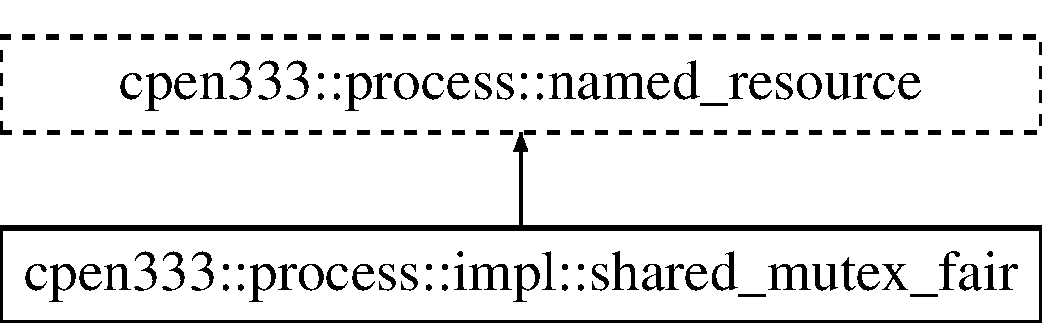
\includegraphics[height=2.000000cm]{classcpen333_1_1process_1_1impl_1_1shared__mutex__fair}
\end{center}
\end{figure}
\subsection*{Public Member Functions}
\begin{DoxyCompactItemize}
\item 
\hyperlink{classcpen333_1_1process_1_1impl_1_1shared__mutex__fair_a4a46bce7595b9f2a29067723f3b72b5e}{shared\+\_\+mutex\+\_\+fair} (const std\+::string \&name)
\begin{DoxyCompactList}\small\item\em Constructor, creates a fair shared mutex. \end{DoxyCompactList}\item 
\mbox{\Hypertarget{classcpen333_1_1process_1_1impl_1_1shared__mutex__fair_a9660ca9c813290ded68578cf5175d966}\label{classcpen333_1_1process_1_1impl_1_1shared__mutex__fair_a9660ca9c813290ded68578cf5175d966}} 
{\bfseries shared\+\_\+mutex\+\_\+fair} (const \hyperlink{classcpen333_1_1process_1_1impl_1_1shared__mutex__fair}{shared\+\_\+mutex\+\_\+fair} \&)=delete
\item 
\mbox{\Hypertarget{classcpen333_1_1process_1_1impl_1_1shared__mutex__fair_a9b61874654e45ccff9ee06c841e6e0a4}\label{classcpen333_1_1process_1_1impl_1_1shared__mutex__fair_a9b61874654e45ccff9ee06c841e6e0a4}} 
{\bfseries shared\+\_\+mutex\+\_\+fair} (\hyperlink{classcpen333_1_1process_1_1impl_1_1shared__mutex__fair}{shared\+\_\+mutex\+\_\+fair} \&\&)=delete
\item 
\mbox{\Hypertarget{classcpen333_1_1process_1_1impl_1_1shared__mutex__fair_a68d7923baa7fe01d8109d61cb4fec8d9}\label{classcpen333_1_1process_1_1impl_1_1shared__mutex__fair_a68d7923baa7fe01d8109d61cb4fec8d9}} 
\hyperlink{classcpen333_1_1process_1_1impl_1_1shared__mutex__fair}{shared\+\_\+mutex\+\_\+fair} \& {\bfseries operator=} (const \hyperlink{classcpen333_1_1process_1_1impl_1_1shared__mutex__fair}{shared\+\_\+mutex\+\_\+fair} \&)=delete
\item 
\mbox{\Hypertarget{classcpen333_1_1process_1_1impl_1_1shared__mutex__fair_a282afc005f687935cb75f9cea0dbbb81}\label{classcpen333_1_1process_1_1impl_1_1shared__mutex__fair_a282afc005f687935cb75f9cea0dbbb81}} 
\hyperlink{classcpen333_1_1process_1_1impl_1_1shared__mutex__fair}{shared\+\_\+mutex\+\_\+fair} \& {\bfseries operator=} (\hyperlink{classcpen333_1_1process_1_1impl_1_1shared__mutex__fair}{shared\+\_\+mutex\+\_\+fair} \&\&)=delete
\item 
void \hyperlink{classcpen333_1_1process_1_1impl_1_1shared__mutex__fair_a11641159a61a83eda9713891f9f29159}{lock\+\_\+shared} ()
\begin{DoxyCompactList}\small\item\em Lock the mutex in shared access mode. \end{DoxyCompactList}\item 
bool \hyperlink{classcpen333_1_1process_1_1impl_1_1shared__mutex__fair_a1d1a77e135745777f6476fe0abcca078}{try\+\_\+lock\+\_\+shared} ()
\begin{DoxyCompactList}\small\item\em Tries to lock the mutex in shared access mode. \end{DoxyCompactList}\item 
void \hyperlink{classcpen333_1_1process_1_1impl_1_1shared__mutex__fair_afa970da78252148b1ff049be3c239155}{unlock\+\_\+shared} ()
\begin{DoxyCompactList}\small\item\em Unlocks one instance of shared access. \end{DoxyCompactList}\item 
void \hyperlink{classcpen333_1_1process_1_1impl_1_1shared__mutex__fair_a85de84ee97bdf015411169a02935dc4d}{lock} ()
\begin{DoxyCompactList}\small\item\em Locks the mutex in exclusive access mode. \end{DoxyCompactList}\item 
bool \hyperlink{classcpen333_1_1process_1_1impl_1_1shared__mutex__fair_aaac6ea293ec760cb35eefeb004503e9a}{try\+\_\+lock} ()
\begin{DoxyCompactList}\small\item\em Tries to lock the mutex in exclusive access mode. \end{DoxyCompactList}\item 
void \hyperlink{classcpen333_1_1process_1_1impl_1_1shared__mutex__fair_a52f1959d5dfe0c08b911e0c4b06ce61c}{unlock} ()
\begin{DoxyCompactList}\small\item\em Unlocks the exclusively-\/locked mutex. \end{DoxyCompactList}\item 
{\footnotesize template$<$class Rep , class Period $>$ }\\bool \hyperlink{classcpen333_1_1process_1_1impl_1_1shared__mutex__fair_a949f9ed2c12c14bd2cade7ec96dd3adb}{try\+\_\+lock\+\_\+for} (const std\+::chrono\+::duration$<$ Rep, Period $>$ \&timeout\+\_\+duration)
\begin{DoxyCompactList}\small\item\em Try to exclusively lock the mutex, with a relative timeout. \end{DoxyCompactList}\item 
{\footnotesize template$<$class Clock , class Duration $>$ }\\bool \hyperlink{classcpen333_1_1process_1_1impl_1_1shared__mutex__fair_ab8acef917db5784868e439a26a72343b}{try\+\_\+lock\+\_\+until} (const std\+::chrono\+::time\+\_\+point$<$ Clock, Duration $>$ \&timeout\+\_\+time)
\begin{DoxyCompactList}\small\item\em Try to exclusively lock the mutex, within an absolute timeout period. \end{DoxyCompactList}\item 
{\footnotesize template$<$class Rep , class Period $>$ }\\bool \hyperlink{classcpen333_1_1process_1_1impl_1_1shared__mutex__fair_a0927a5897a261f5eb992eb442145fdf5}{try\+\_\+lock\+\_\+shared\+\_\+for} (const std\+::chrono\+::duration$<$ Rep, Period $>$ \&timeout\+\_\+duration)
\begin{DoxyCompactList}\small\item\em Try to lock the mutex in shared mode, with a relative timeout. \end{DoxyCompactList}\item 
{\footnotesize template$<$class Clock , class Duration $>$ }\\bool \hyperlink{classcpen333_1_1process_1_1impl_1_1shared__mutex__fair_af45bf5f8271a18b7cf3e737288d38025}{try\+\_\+lock\+\_\+shared\+\_\+until} (const std\+::chrono\+::time\+\_\+point$<$ Clock, Duration $>$ \&timeout\+\_\+time)
\begin{DoxyCompactList}\small\item\em Try to lock the mutex in shared mode, with absolute timeout. \end{DoxyCompactList}\item 
bool \hyperlink{classcpen333_1_1process_1_1impl_1_1shared__mutex__fair_a40e20137e0c27f4a742ab6c5388eb61b}{unlink} ()
\begin{DoxyCompactList}\small\item\em Detaches the name from the named resource. \end{DoxyCompactList}\end{DoxyCompactItemize}
\subsection*{Static Public Member Functions}
\begin{DoxyCompactItemize}
\item 
static bool \hyperlink{classcpen333_1_1process_1_1impl_1_1shared__mutex__fair_a956a4efec20df5852fef56bfd2a22ea2}{unlink} (const std\+::string \&name)
\begin{DoxyCompactList}\small\item\em Unlinks the name without needing to create a resource. \end{DoxyCompactList}\end{DoxyCompactItemize}


\subsection{Detailed Description}
An inter-\/process shared mutex implementation with balanced priorities. 

A more fair shared mutex, access is granted in batches\+: 1 writer, batch of readers, 1 writer, batch of readers Based on the alternating method described here\+: \href{http://www.tools-of-computing.com/tc/CS/Monitors/AlternatingRW.htm}{\tt http\+://www.\+tools-\/of-\/computing.\+com/tc/\+C\+S/\+Monitors/\+Alternating\+R\+W.\+htm} 

\subsection{Constructor \& Destructor Documentation}
\mbox{\Hypertarget{classcpen333_1_1process_1_1impl_1_1shared__mutex__fair_a4a46bce7595b9f2a29067723f3b72b5e}\label{classcpen333_1_1process_1_1impl_1_1shared__mutex__fair_a4a46bce7595b9f2a29067723f3b72b5e}} 
\index{cpen333\+::process\+::impl\+::shared\+\_\+mutex\+\_\+fair@{cpen333\+::process\+::impl\+::shared\+\_\+mutex\+\_\+fair}!shared\+\_\+mutex\+\_\+fair@{shared\+\_\+mutex\+\_\+fair}}
\index{shared\+\_\+mutex\+\_\+fair@{shared\+\_\+mutex\+\_\+fair}!cpen333\+::process\+::impl\+::shared\+\_\+mutex\+\_\+fair@{cpen333\+::process\+::impl\+::shared\+\_\+mutex\+\_\+fair}}
\subsubsection{\texorpdfstring{shared\+\_\+mutex\+\_\+fair()}{shared\_mutex\_fair()}}
{\footnotesize\ttfamily cpen333\+::process\+::impl\+::shared\+\_\+mutex\+\_\+fair\+::shared\+\_\+mutex\+\_\+fair (\begin{DoxyParamCaption}\item[{const std\+::string \&}]{name }\end{DoxyParamCaption})\hspace{0.3cm}{\ttfamily [inline]}}



Constructor, creates a fair shared mutex. 


\begin{DoxyParams}{Parameters}
{\em name} & identifier for creating or connecting to an existing inter-\/process shared mutex \\
\hline
\end{DoxyParams}


\subsection{Member Function Documentation}
\mbox{\Hypertarget{classcpen333_1_1process_1_1impl_1_1shared__mutex__fair_a85de84ee97bdf015411169a02935dc4d}\label{classcpen333_1_1process_1_1impl_1_1shared__mutex__fair_a85de84ee97bdf015411169a02935dc4d}} 
\index{cpen333\+::process\+::impl\+::shared\+\_\+mutex\+\_\+fair@{cpen333\+::process\+::impl\+::shared\+\_\+mutex\+\_\+fair}!lock@{lock}}
\index{lock@{lock}!cpen333\+::process\+::impl\+::shared\+\_\+mutex\+\_\+fair@{cpen333\+::process\+::impl\+::shared\+\_\+mutex\+\_\+fair}}
\subsubsection{\texorpdfstring{lock()}{lock()}}
{\footnotesize\ttfamily void cpen333\+::process\+::impl\+::shared\+\_\+mutex\+\_\+fair\+::lock (\begin{DoxyParamCaption}{ }\end{DoxyParamCaption})\hspace{0.3cm}{\ttfamily [inline]}}



Locks the mutex in exclusive access mode. 

Only one thread can lock in exclusive access mode. This method will block if the mutex is currently locked in either shared or exclusive mode. \mbox{\Hypertarget{classcpen333_1_1process_1_1impl_1_1shared__mutex__fair_a11641159a61a83eda9713891f9f29159}\label{classcpen333_1_1process_1_1impl_1_1shared__mutex__fair_a11641159a61a83eda9713891f9f29159}} 
\index{cpen333\+::process\+::impl\+::shared\+\_\+mutex\+\_\+fair@{cpen333\+::process\+::impl\+::shared\+\_\+mutex\+\_\+fair}!lock\+\_\+shared@{lock\+\_\+shared}}
\index{lock\+\_\+shared@{lock\+\_\+shared}!cpen333\+::process\+::impl\+::shared\+\_\+mutex\+\_\+fair@{cpen333\+::process\+::impl\+::shared\+\_\+mutex\+\_\+fair}}
\subsubsection{\texorpdfstring{lock\+\_\+shared()}{lock\_shared()}}
{\footnotesize\ttfamily void cpen333\+::process\+::impl\+::shared\+\_\+mutex\+\_\+fair\+::lock\+\_\+shared (\begin{DoxyParamCaption}{ }\end{DoxyParamCaption})\hspace{0.3cm}{\ttfamily [inline]}}



Lock the mutex in shared access mode. 

Multiple threads can lock in shared mode concurrently, allowing simultaneous access. This method will block if the mutex is currently locked in exclusive mode. \mbox{\Hypertarget{classcpen333_1_1process_1_1impl_1_1shared__mutex__fair_aaac6ea293ec760cb35eefeb004503e9a}\label{classcpen333_1_1process_1_1impl_1_1shared__mutex__fair_aaac6ea293ec760cb35eefeb004503e9a}} 
\index{cpen333\+::process\+::impl\+::shared\+\_\+mutex\+\_\+fair@{cpen333\+::process\+::impl\+::shared\+\_\+mutex\+\_\+fair}!try\+\_\+lock@{try\+\_\+lock}}
\index{try\+\_\+lock@{try\+\_\+lock}!cpen333\+::process\+::impl\+::shared\+\_\+mutex\+\_\+fair@{cpen333\+::process\+::impl\+::shared\+\_\+mutex\+\_\+fair}}
\subsubsection{\texorpdfstring{try\+\_\+lock()}{try\_lock()}}
{\footnotesize\ttfamily bool cpen333\+::process\+::impl\+::shared\+\_\+mutex\+\_\+fair\+::try\+\_\+lock (\begin{DoxyParamCaption}{ }\end{DoxyParamCaption})\hspace{0.3cm}{\ttfamily [inline]}}



Tries to lock the mutex in exclusive access mode. 

Only one thread can lock in exclusive access mode. This method returns immediately.

\begin{DoxyReturn}{Returns}
true if successfully locked, false if already locked in either shared or exclusive access mode 
\end{DoxyReturn}
\mbox{\Hypertarget{classcpen333_1_1process_1_1impl_1_1shared__mutex__fair_a949f9ed2c12c14bd2cade7ec96dd3adb}\label{classcpen333_1_1process_1_1impl_1_1shared__mutex__fair_a949f9ed2c12c14bd2cade7ec96dd3adb}} 
\index{cpen333\+::process\+::impl\+::shared\+\_\+mutex\+\_\+fair@{cpen333\+::process\+::impl\+::shared\+\_\+mutex\+\_\+fair}!try\+\_\+lock\+\_\+for@{try\+\_\+lock\+\_\+for}}
\index{try\+\_\+lock\+\_\+for@{try\+\_\+lock\+\_\+for}!cpen333\+::process\+::impl\+::shared\+\_\+mutex\+\_\+fair@{cpen333\+::process\+::impl\+::shared\+\_\+mutex\+\_\+fair}}
\subsubsection{\texorpdfstring{try\+\_\+lock\+\_\+for()}{try\_lock\_for()}}
{\footnotesize\ttfamily template$<$class Rep , class Period $>$ \\
bool cpen333\+::process\+::impl\+::shared\+\_\+mutex\+\_\+fair\+::try\+\_\+lock\+\_\+for (\begin{DoxyParamCaption}\item[{const std\+::chrono\+::duration$<$ Rep, Period $>$ \&}]{timeout\+\_\+duration }\end{DoxyParamCaption})\hspace{0.3cm}{\ttfamily [inline]}}



Try to exclusively lock the mutex, with a relative timeout. 

Tries to lock the mutex in exclusive-\/access (write) mode, returns if the mutex has been unavailable for the specified timeout duration


\begin{DoxyTemplParams}{Template Parameters}
{\em Rep} & duration representation \\
\hline
{\em Period} & duration period \\
\hline
\end{DoxyTemplParams}

\begin{DoxyParams}{Parameters}
{\em timeout\+\_\+duration} & timeout duration \\
\hline
\end{DoxyParams}
\begin{DoxyReturn}{Returns}
true if locked successfully 
\end{DoxyReturn}
\mbox{\Hypertarget{classcpen333_1_1process_1_1impl_1_1shared__mutex__fair_a1d1a77e135745777f6476fe0abcca078}\label{classcpen333_1_1process_1_1impl_1_1shared__mutex__fair_a1d1a77e135745777f6476fe0abcca078}} 
\index{cpen333\+::process\+::impl\+::shared\+\_\+mutex\+\_\+fair@{cpen333\+::process\+::impl\+::shared\+\_\+mutex\+\_\+fair}!try\+\_\+lock\+\_\+shared@{try\+\_\+lock\+\_\+shared}}
\index{try\+\_\+lock\+\_\+shared@{try\+\_\+lock\+\_\+shared}!cpen333\+::process\+::impl\+::shared\+\_\+mutex\+\_\+fair@{cpen333\+::process\+::impl\+::shared\+\_\+mutex\+\_\+fair}}
\subsubsection{\texorpdfstring{try\+\_\+lock\+\_\+shared()}{try\_lock\_shared()}}
{\footnotesize\ttfamily bool cpen333\+::process\+::impl\+::shared\+\_\+mutex\+\_\+fair\+::try\+\_\+lock\+\_\+shared (\begin{DoxyParamCaption}{ }\end{DoxyParamCaption})\hspace{0.3cm}{\ttfamily [inline]}}



Tries to lock the mutex in shared access mode. 

Multiple threads can lock in shared mode concurrently, allowing simultaneous access. This method returns immediately.

\begin{DoxyReturn}{Returns}
true if successfully locked, false if mutex is currently locked in exclusive access mode 
\end{DoxyReturn}
\mbox{\Hypertarget{classcpen333_1_1process_1_1impl_1_1shared__mutex__fair_a0927a5897a261f5eb992eb442145fdf5}\label{classcpen333_1_1process_1_1impl_1_1shared__mutex__fair_a0927a5897a261f5eb992eb442145fdf5}} 
\index{cpen333\+::process\+::impl\+::shared\+\_\+mutex\+\_\+fair@{cpen333\+::process\+::impl\+::shared\+\_\+mutex\+\_\+fair}!try\+\_\+lock\+\_\+shared\+\_\+for@{try\+\_\+lock\+\_\+shared\+\_\+for}}
\index{try\+\_\+lock\+\_\+shared\+\_\+for@{try\+\_\+lock\+\_\+shared\+\_\+for}!cpen333\+::process\+::impl\+::shared\+\_\+mutex\+\_\+fair@{cpen333\+::process\+::impl\+::shared\+\_\+mutex\+\_\+fair}}
\subsubsection{\texorpdfstring{try\+\_\+lock\+\_\+shared\+\_\+for()}{try\_lock\_shared\_for()}}
{\footnotesize\ttfamily template$<$class Rep , class Period $>$ \\
bool cpen333\+::process\+::impl\+::shared\+\_\+mutex\+\_\+fair\+::try\+\_\+lock\+\_\+shared\+\_\+for (\begin{DoxyParamCaption}\item[{const std\+::chrono\+::duration$<$ Rep, Period $>$ \&}]{timeout\+\_\+duration }\end{DoxyParamCaption})\hspace{0.3cm}{\ttfamily [inline]}}



Try to lock the mutex in shared mode, with a relative timeout. 

Tries to lock the mutex in shared-\/access (read) mode, returns if the mutex has been unavailable for the specified timeout duration


\begin{DoxyTemplParams}{Template Parameters}
{\em Rep} & duration representation \\
\hline
{\em Period} & duration period \\
\hline
\end{DoxyTemplParams}

\begin{DoxyParams}{Parameters}
{\em timeout\+\_\+duration} & timeout duration \\
\hline
\end{DoxyParams}
\begin{DoxyReturn}{Returns}
true if locked successfully 
\end{DoxyReturn}
\mbox{\Hypertarget{classcpen333_1_1process_1_1impl_1_1shared__mutex__fair_af45bf5f8271a18b7cf3e737288d38025}\label{classcpen333_1_1process_1_1impl_1_1shared__mutex__fair_af45bf5f8271a18b7cf3e737288d38025}} 
\index{cpen333\+::process\+::impl\+::shared\+\_\+mutex\+\_\+fair@{cpen333\+::process\+::impl\+::shared\+\_\+mutex\+\_\+fair}!try\+\_\+lock\+\_\+shared\+\_\+until@{try\+\_\+lock\+\_\+shared\+\_\+until}}
\index{try\+\_\+lock\+\_\+shared\+\_\+until@{try\+\_\+lock\+\_\+shared\+\_\+until}!cpen333\+::process\+::impl\+::shared\+\_\+mutex\+\_\+fair@{cpen333\+::process\+::impl\+::shared\+\_\+mutex\+\_\+fair}}
\subsubsection{\texorpdfstring{try\+\_\+lock\+\_\+shared\+\_\+until()}{try\_lock\_shared\_until()}}
{\footnotesize\ttfamily template$<$class Clock , class Duration $>$ \\
bool cpen333\+::process\+::impl\+::shared\+\_\+mutex\+\_\+fair\+::try\+\_\+lock\+\_\+shared\+\_\+until (\begin{DoxyParamCaption}\item[{const std\+::chrono\+::time\+\_\+point$<$ Clock, Duration $>$ \&}]{timeout\+\_\+time }\end{DoxyParamCaption})\hspace{0.3cm}{\ttfamily [inline]}}



Try to lock the mutex in shared mode, with absolute timeout. 

Tries to lock the mutex in shared-\/access (read) mode, returns if the mutex has been unavailable until specified time point has been reached


\begin{DoxyTemplParams}{Template Parameters}
{\em Clock} & clock representation \\
\hline
{\em Duration} & time \\
\hline
\end{DoxyTemplParams}

\begin{DoxyParams}{Parameters}
{\em timeout\+\_\+time} & time of timeout \\
\hline
\end{DoxyParams}
\begin{DoxyReturn}{Returns}
true if locked successfully 
\end{DoxyReturn}
\mbox{\Hypertarget{classcpen333_1_1process_1_1impl_1_1shared__mutex__fair_ab8acef917db5784868e439a26a72343b}\label{classcpen333_1_1process_1_1impl_1_1shared__mutex__fair_ab8acef917db5784868e439a26a72343b}} 
\index{cpen333\+::process\+::impl\+::shared\+\_\+mutex\+\_\+fair@{cpen333\+::process\+::impl\+::shared\+\_\+mutex\+\_\+fair}!try\+\_\+lock\+\_\+until@{try\+\_\+lock\+\_\+until}}
\index{try\+\_\+lock\+\_\+until@{try\+\_\+lock\+\_\+until}!cpen333\+::process\+::impl\+::shared\+\_\+mutex\+\_\+fair@{cpen333\+::process\+::impl\+::shared\+\_\+mutex\+\_\+fair}}
\subsubsection{\texorpdfstring{try\+\_\+lock\+\_\+until()}{try\_lock\_until()}}
{\footnotesize\ttfamily template$<$class Clock , class Duration $>$ \\
bool cpen333\+::process\+::impl\+::shared\+\_\+mutex\+\_\+fair\+::try\+\_\+lock\+\_\+until (\begin{DoxyParamCaption}\item[{const std\+::chrono\+::time\+\_\+point$<$ Clock, Duration $>$ \&}]{timeout\+\_\+time }\end{DoxyParamCaption})\hspace{0.3cm}{\ttfamily [inline]}}



Try to exclusively lock the mutex, within an absolute timeout period. 

Tries to lock the mutex in exclusive-\/access (write) mode, returns if the mutex has been unavailable until specified time point has been reached


\begin{DoxyTemplParams}{Template Parameters}
{\em Clock} & clock representation \\
\hline
{\em Duration} & time \\
\hline
\end{DoxyTemplParams}

\begin{DoxyParams}{Parameters}
{\em timeout\+\_\+time} & time of timeout \\
\hline
\end{DoxyParams}
\begin{DoxyReturn}{Returns}
true if locked successfully 
\end{DoxyReturn}
\mbox{\Hypertarget{classcpen333_1_1process_1_1impl_1_1shared__mutex__fair_a40e20137e0c27f4a742ab6c5388eb61b}\label{classcpen333_1_1process_1_1impl_1_1shared__mutex__fair_a40e20137e0c27f4a742ab6c5388eb61b}} 
\index{cpen333\+::process\+::impl\+::shared\+\_\+mutex\+\_\+fair@{cpen333\+::process\+::impl\+::shared\+\_\+mutex\+\_\+fair}!unlink@{unlink}}
\index{unlink@{unlink}!cpen333\+::process\+::impl\+::shared\+\_\+mutex\+\_\+fair@{cpen333\+::process\+::impl\+::shared\+\_\+mutex\+\_\+fair}}
\subsubsection{\texorpdfstring{unlink()}{unlink()}\hspace{0.1cm}{\footnotesize\ttfamily [1/2]}}
{\footnotesize\ttfamily bool cpen333\+::process\+::impl\+::shared\+\_\+mutex\+\_\+fair\+::unlink (\begin{DoxyParamCaption}{ }\end{DoxyParamCaption})\hspace{0.3cm}{\ttfamily [inline]}, {\ttfamily [virtual]}}



Detaches the name from the named resource. 

On P\+O\+S\+IX systems, named resources will persist beyond the lifetime of any process that uses them as long as the name has not been unlinked (or until the system is rebooted). Calling {\ttfamily unlink} will detach the name, allowing the resource to be freed once all current users have exited.

\begin{DoxyReturn}{Returns}
{\ttfamily true} if unlink is successful, {\ttfamily false} if unlinking is not supported or if an error has occurred. 
\end{DoxyReturn}


Implements \hyperlink{classcpen333_1_1process_1_1named__resource_a5d33168fee48c9b0c58ab8fd96e230ce}{cpen333\+::process\+::named\+\_\+resource}.

\mbox{\Hypertarget{classcpen333_1_1process_1_1impl_1_1shared__mutex__fair_a956a4efec20df5852fef56bfd2a22ea2}\label{classcpen333_1_1process_1_1impl_1_1shared__mutex__fair_a956a4efec20df5852fef56bfd2a22ea2}} 
\index{cpen333\+::process\+::impl\+::shared\+\_\+mutex\+\_\+fair@{cpen333\+::process\+::impl\+::shared\+\_\+mutex\+\_\+fair}!unlink@{unlink}}
\index{unlink@{unlink}!cpen333\+::process\+::impl\+::shared\+\_\+mutex\+\_\+fair@{cpen333\+::process\+::impl\+::shared\+\_\+mutex\+\_\+fair}}
\subsubsection{\texorpdfstring{unlink()}{unlink()}\hspace{0.1cm}{\footnotesize\ttfamily [2/2]}}
{\footnotesize\ttfamily static bool cpen333\+::process\+::impl\+::shared\+\_\+mutex\+\_\+fair\+::unlink (\begin{DoxyParamCaption}\item[{const std\+::string \&}]{name }\end{DoxyParamCaption})\hspace{0.3cm}{\ttfamily [inline]}, {\ttfamily [static]}}



Unlinks the name without needing to create a resource. 

Implementers should also provide a static method for unlinking. The purpose is mainly for clean-\/up of existing resources.


\begin{DoxyParams}{Parameters}
{\em name} & desired resource name \\
\hline
\end{DoxyParams}
\begin{DoxyReturn}{Returns}
{\ttfamily true} if unlink successful, {\ttfamily false} if not successful or not supported 
\end{DoxyReturn}
\mbox{\Hypertarget{classcpen333_1_1process_1_1impl_1_1shared__mutex__fair_a52f1959d5dfe0c08b911e0c4b06ce61c}\label{classcpen333_1_1process_1_1impl_1_1shared__mutex__fair_a52f1959d5dfe0c08b911e0c4b06ce61c}} 
\index{cpen333\+::process\+::impl\+::shared\+\_\+mutex\+\_\+fair@{cpen333\+::process\+::impl\+::shared\+\_\+mutex\+\_\+fair}!unlock@{unlock}}
\index{unlock@{unlock}!cpen333\+::process\+::impl\+::shared\+\_\+mutex\+\_\+fair@{cpen333\+::process\+::impl\+::shared\+\_\+mutex\+\_\+fair}}
\subsubsection{\texorpdfstring{unlock()}{unlock()}}
{\footnotesize\ttfamily void cpen333\+::process\+::impl\+::shared\+\_\+mutex\+\_\+fair\+::unlock (\begin{DoxyParamCaption}{ }\end{DoxyParamCaption})\hspace{0.3cm}{\ttfamily [inline]}}



Unlocks the exclusively-\/locked mutex. 

\mbox{\Hypertarget{classcpen333_1_1process_1_1impl_1_1shared__mutex__fair_afa970da78252148b1ff049be3c239155}\label{classcpen333_1_1process_1_1impl_1_1shared__mutex__fair_afa970da78252148b1ff049be3c239155}} 
\index{cpen333\+::process\+::impl\+::shared\+\_\+mutex\+\_\+fair@{cpen333\+::process\+::impl\+::shared\+\_\+mutex\+\_\+fair}!unlock\+\_\+shared@{unlock\+\_\+shared}}
\index{unlock\+\_\+shared@{unlock\+\_\+shared}!cpen333\+::process\+::impl\+::shared\+\_\+mutex\+\_\+fair@{cpen333\+::process\+::impl\+::shared\+\_\+mutex\+\_\+fair}}
\subsubsection{\texorpdfstring{unlock\+\_\+shared()}{unlock\_shared()}}
{\footnotesize\ttfamily void cpen333\+::process\+::impl\+::shared\+\_\+mutex\+\_\+fair\+::unlock\+\_\+shared (\begin{DoxyParamCaption}{ }\end{DoxyParamCaption})\hspace{0.3cm}{\ttfamily [inline]}}



Unlocks one instance of shared access. 

The mutex will continue to remain locked in shared access mode until all shared locks are unlocked. 

The documentation for this class was generated from the following file\+:\begin{DoxyCompactItemize}
\item 
D\+:/school/teaching/\+C\+P\+E\+N333/workspace/labs/include/cpen333/process/impl/\hyperlink{shared__mutex__fair_8h}{shared\+\_\+mutex\+\_\+fair.\+h}\end{DoxyCompactItemize}

\hypertarget{classcpen333_1_1process_1_1impl_1_1shared__mutex__shared}{}\section{cpen333\+:\+:process\+:\+:impl\+:\+:shared\+\_\+mutex\+\_\+shared Class Reference}
\label{classcpen333_1_1process_1_1impl_1_1shared__mutex__shared}\index{cpen333\+::process\+::impl\+::shared\+\_\+mutex\+\_\+shared@{cpen333\+::process\+::impl\+::shared\+\_\+mutex\+\_\+shared}}


A read-\/preferring inter-\/process shared mutex implementation.  




{\ttfamily \#include $<$shared\+\_\+mutex\+\_\+shared.\+h$>$}

Inheritance diagram for cpen333\+:\+:process\+:\+:impl\+:\+:shared\+\_\+mutex\+\_\+shared\+:\begin{figure}[H]
\begin{center}
\leavevmode
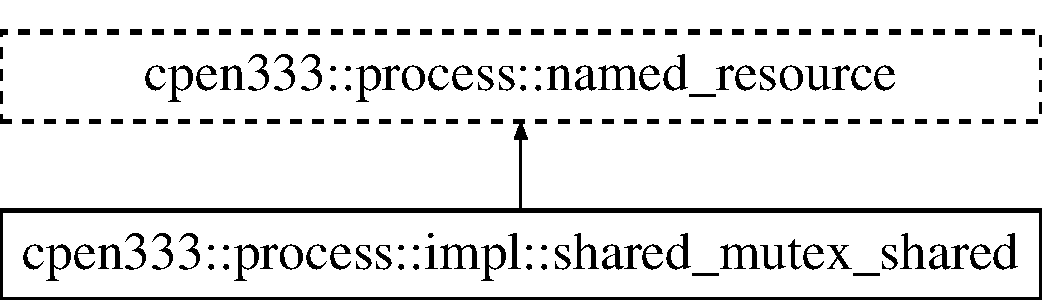
\includegraphics[height=2.000000cm]{classcpen333_1_1process_1_1impl_1_1shared__mutex__shared}
\end{center}
\end{figure}
\subsection*{Public Member Functions}
\begin{DoxyCompactItemize}
\item 
\hyperlink{classcpen333_1_1process_1_1impl_1_1shared__mutex__shared_aa94fee843eb846e57c4ac51589172849}{shared\+\_\+mutex\+\_\+shared} (const std\+::string \&name)
\item 
\mbox{\Hypertarget{classcpen333_1_1process_1_1impl_1_1shared__mutex__shared_a1a1a4c997212a30de0acffdb151a6784}\label{classcpen333_1_1process_1_1impl_1_1shared__mutex__shared_a1a1a4c997212a30de0acffdb151a6784}} 
{\bfseries shared\+\_\+mutex\+\_\+shared} (const \hyperlink{classcpen333_1_1process_1_1impl_1_1shared__mutex__shared}{shared\+\_\+mutex\+\_\+shared} \&)=delete
\item 
\mbox{\Hypertarget{classcpen333_1_1process_1_1impl_1_1shared__mutex__shared_aeb8440ba1ac5d0f4976f592ca22af915}\label{classcpen333_1_1process_1_1impl_1_1shared__mutex__shared_aeb8440ba1ac5d0f4976f592ca22af915}} 
{\bfseries shared\+\_\+mutex\+\_\+shared} (\hyperlink{classcpen333_1_1process_1_1impl_1_1shared__mutex__shared}{shared\+\_\+mutex\+\_\+shared} \&\&)=delete
\item 
\mbox{\Hypertarget{classcpen333_1_1process_1_1impl_1_1shared__mutex__shared_af749d860d3161ffe5a5f0059f47b3e6a}\label{classcpen333_1_1process_1_1impl_1_1shared__mutex__shared_af749d860d3161ffe5a5f0059f47b3e6a}} 
\hyperlink{classcpen333_1_1process_1_1impl_1_1shared__mutex__shared}{shared\+\_\+mutex\+\_\+shared} \& {\bfseries operator=} (const \hyperlink{classcpen333_1_1process_1_1impl_1_1shared__mutex__shared}{shared\+\_\+mutex\+\_\+shared} \&)=delete
\item 
\mbox{\Hypertarget{classcpen333_1_1process_1_1impl_1_1shared__mutex__shared_afe0a4dae3afe6aa50ab7917c78369486}\label{classcpen333_1_1process_1_1impl_1_1shared__mutex__shared_afe0a4dae3afe6aa50ab7917c78369486}} 
\hyperlink{classcpen333_1_1process_1_1impl_1_1shared__mutex__shared}{shared\+\_\+mutex\+\_\+shared} \& {\bfseries operator=} (\hyperlink{classcpen333_1_1process_1_1impl_1_1shared__mutex__shared}{shared\+\_\+mutex\+\_\+shared} \&\&)=delete
\item 
void \hyperlink{classcpen333_1_1process_1_1impl_1_1shared__mutex__shared_a29036d76ee3f41ae157bb87b4316ea97}{lock\+\_\+shared} ()
\begin{DoxyCompactList}\small\item\em Lock the mutex in shared access mode. \end{DoxyCompactList}\item 
bool \hyperlink{classcpen333_1_1process_1_1impl_1_1shared__mutex__shared_a382dfc90cc323e70879de8e69bcb7e24}{try\+\_\+lock\+\_\+shared} ()
\begin{DoxyCompactList}\small\item\em Tries to lock the mutex in shared access mode. \end{DoxyCompactList}\item 
void \hyperlink{classcpen333_1_1process_1_1impl_1_1shared__mutex__shared_a4a7331e891ef08ffddda51ab5722fac6}{unlock\+\_\+shared} ()
\begin{DoxyCompactList}\small\item\em Unlocks one instance of shared access. \end{DoxyCompactList}\item 
void \hyperlink{classcpen333_1_1process_1_1impl_1_1shared__mutex__shared_a48a55c1a0bc4465ce3042eac361b674c}{lock} ()
\begin{DoxyCompactList}\small\item\em Locks the mutex in exclusive access mode. \end{DoxyCompactList}\item 
bool \hyperlink{classcpen333_1_1process_1_1impl_1_1shared__mutex__shared_a14e358b1ecbdebd69fb89fdc3b2a4f61}{try\+\_\+lock} ()
\begin{DoxyCompactList}\small\item\em Tries to lock the mutex in exclusive access mode. \end{DoxyCompactList}\item 
void \hyperlink{classcpen333_1_1process_1_1impl_1_1shared__mutex__shared_aa5a87d5886497263cc6b0f0a4d79f15c}{unlock} ()
\begin{DoxyCompactList}\small\item\em Unlocks the exclusively-\/locked mutex. \end{DoxyCompactList}\item 
{\footnotesize template$<$class Rep , class Period $>$ }\\bool \hyperlink{classcpen333_1_1process_1_1impl_1_1shared__mutex__shared_a4437c703911edfa03d9cc759fbc6f9c3}{try\+\_\+lock\+\_\+for} (const std\+::chrono\+::duration$<$ Rep, Period $>$ \&timeout\+\_\+duration)
\begin{DoxyCompactList}\small\item\em Try to exclusively lock the mutex, with a relative timeout. \end{DoxyCompactList}\item 
{\footnotesize template$<$class Clock , class Duration $>$ }\\bool \hyperlink{classcpen333_1_1process_1_1impl_1_1shared__mutex__shared_a3aeb0499325e4a073de1877f0a41f2bb}{try\+\_\+lock\+\_\+until} (const std\+::chrono\+::time\+\_\+point$<$ Clock, Duration $>$ \&timeout\+\_\+time)
\begin{DoxyCompactList}\small\item\em Try to exclusively lock the mutex, within an absolute timeout period. \end{DoxyCompactList}\item 
{\footnotesize template$<$class Rep , class Period $>$ }\\bool \hyperlink{classcpen333_1_1process_1_1impl_1_1shared__mutex__shared_a14203d4013d62fed7e1a8904c0db3793}{try\+\_\+lock\+\_\+shared\+\_\+for} (const std\+::chrono\+::duration$<$ Rep, Period $>$ \&timeout\+\_\+duration)
\begin{DoxyCompactList}\small\item\em Try to lock the mutex in shared mode, with a relative timeout. \end{DoxyCompactList}\item 
{\footnotesize template$<$class Clock , class Duration $>$ }\\bool \hyperlink{classcpen333_1_1process_1_1impl_1_1shared__mutex__shared_a25bf54e2064e78bc18e996dacb082f3c}{try\+\_\+lock\+\_\+shared\+\_\+until} (const std\+::chrono\+::time\+\_\+point$<$ Clock, Duration $>$ \&timeout\+\_\+time)
\begin{DoxyCompactList}\small\item\em Try to lock the mutex in shared mode, with absolute timeout. \end{DoxyCompactList}\item 
bool \hyperlink{classcpen333_1_1process_1_1impl_1_1shared__mutex__shared_a8e6c759f5d5266b931ed78da04652d61}{unlink} ()
\begin{DoxyCompactList}\small\item\em Detaches the name from the named resource. \end{DoxyCompactList}\end{DoxyCompactItemize}
\subsection*{Static Public Member Functions}
\begin{DoxyCompactItemize}
\item 
static bool \hyperlink{classcpen333_1_1process_1_1impl_1_1shared__mutex__shared_a855882d87dd04246229b624179837030}{unlink} (const std\+::string \&name)
\begin{DoxyCompactList}\small\item\em Unlinks the name without needing to create a resource. \end{DoxyCompactList}\end{DoxyCompactItemize}


\subsection{Detailed Description}
A read-\/preferring inter-\/process shared mutex implementation. 

Inter-\/process shared mutex implementation based on the mutex/condition variable pattern. Gives priority to shared (read) access.

See \href{https://en.wikipedia.org/wiki/Readers%E2%80%93writer_lock#Using_a_condition_variable_and_a_mutex}{\tt https\+://en.\+wikipedia.\+org/wiki/\+Readers\%\+E2\%80\%93writer\+\_\+lock\#\+Using\+\_\+a\+\_\+condition\+\_\+variable\+\_\+and\+\_\+a\+\_\+mutex} for details 

\subsection{Constructor \& Destructor Documentation}
\mbox{\Hypertarget{classcpen333_1_1process_1_1impl_1_1shared__mutex__shared_aa94fee843eb846e57c4ac51589172849}\label{classcpen333_1_1process_1_1impl_1_1shared__mutex__shared_aa94fee843eb846e57c4ac51589172849}} 
\index{cpen333\+::process\+::impl\+::shared\+\_\+mutex\+\_\+shared@{cpen333\+::process\+::impl\+::shared\+\_\+mutex\+\_\+shared}!shared\+\_\+mutex\+\_\+shared@{shared\+\_\+mutex\+\_\+shared}}
\index{shared\+\_\+mutex\+\_\+shared@{shared\+\_\+mutex\+\_\+shared}!cpen333\+::process\+::impl\+::shared\+\_\+mutex\+\_\+shared@{cpen333\+::process\+::impl\+::shared\+\_\+mutex\+\_\+shared}}
\subsubsection{\texorpdfstring{shared\+\_\+mutex\+\_\+shared()}{shared\_mutex\_shared()}}
{\footnotesize\ttfamily cpen333\+::process\+::impl\+::shared\+\_\+mutex\+\_\+shared\+::shared\+\_\+mutex\+\_\+shared (\begin{DoxyParamCaption}\item[{const std\+::string \&}]{name }\end{DoxyParamCaption})\hspace{0.3cm}{\ttfamily [inline]}}

Constructor, creates or connects to a read-\/preferring shared mutex 
\begin{DoxyParams}{Parameters}
{\em name} & identifier for creating or connecting to an existing inter-\/process shared mutex \\
\hline
\end{DoxyParams}


\subsection{Member Function Documentation}
\mbox{\Hypertarget{classcpen333_1_1process_1_1impl_1_1shared__mutex__shared_a48a55c1a0bc4465ce3042eac361b674c}\label{classcpen333_1_1process_1_1impl_1_1shared__mutex__shared_a48a55c1a0bc4465ce3042eac361b674c}} 
\index{cpen333\+::process\+::impl\+::shared\+\_\+mutex\+\_\+shared@{cpen333\+::process\+::impl\+::shared\+\_\+mutex\+\_\+shared}!lock@{lock}}
\index{lock@{lock}!cpen333\+::process\+::impl\+::shared\+\_\+mutex\+\_\+shared@{cpen333\+::process\+::impl\+::shared\+\_\+mutex\+\_\+shared}}
\subsubsection{\texorpdfstring{lock()}{lock()}}
{\footnotesize\ttfamily void cpen333\+::process\+::impl\+::shared\+\_\+mutex\+\_\+shared\+::lock (\begin{DoxyParamCaption}{ }\end{DoxyParamCaption})\hspace{0.3cm}{\ttfamily [inline]}}



Locks the mutex in exclusive access mode. 

Only one thread can lock in exclusive access mode. This method will block if the mutex is currently locked in either shared or exclusive mode. \mbox{\Hypertarget{classcpen333_1_1process_1_1impl_1_1shared__mutex__shared_a29036d76ee3f41ae157bb87b4316ea97}\label{classcpen333_1_1process_1_1impl_1_1shared__mutex__shared_a29036d76ee3f41ae157bb87b4316ea97}} 
\index{cpen333\+::process\+::impl\+::shared\+\_\+mutex\+\_\+shared@{cpen333\+::process\+::impl\+::shared\+\_\+mutex\+\_\+shared}!lock\+\_\+shared@{lock\+\_\+shared}}
\index{lock\+\_\+shared@{lock\+\_\+shared}!cpen333\+::process\+::impl\+::shared\+\_\+mutex\+\_\+shared@{cpen333\+::process\+::impl\+::shared\+\_\+mutex\+\_\+shared}}
\subsubsection{\texorpdfstring{lock\+\_\+shared()}{lock\_shared()}}
{\footnotesize\ttfamily void cpen333\+::process\+::impl\+::shared\+\_\+mutex\+\_\+shared\+::lock\+\_\+shared (\begin{DoxyParamCaption}{ }\end{DoxyParamCaption})\hspace{0.3cm}{\ttfamily [inline]}}



Lock the mutex in shared access mode. 

Multiple threads can lock in shared mode concurrently, allowing simultaneous access. This method will block if the mutex is currently locked in exclusive mode. \mbox{\Hypertarget{classcpen333_1_1process_1_1impl_1_1shared__mutex__shared_a14e358b1ecbdebd69fb89fdc3b2a4f61}\label{classcpen333_1_1process_1_1impl_1_1shared__mutex__shared_a14e358b1ecbdebd69fb89fdc3b2a4f61}} 
\index{cpen333\+::process\+::impl\+::shared\+\_\+mutex\+\_\+shared@{cpen333\+::process\+::impl\+::shared\+\_\+mutex\+\_\+shared}!try\+\_\+lock@{try\+\_\+lock}}
\index{try\+\_\+lock@{try\+\_\+lock}!cpen333\+::process\+::impl\+::shared\+\_\+mutex\+\_\+shared@{cpen333\+::process\+::impl\+::shared\+\_\+mutex\+\_\+shared}}
\subsubsection{\texorpdfstring{try\+\_\+lock()}{try\_lock()}}
{\footnotesize\ttfamily bool cpen333\+::process\+::impl\+::shared\+\_\+mutex\+\_\+shared\+::try\+\_\+lock (\begin{DoxyParamCaption}{ }\end{DoxyParamCaption})\hspace{0.3cm}{\ttfamily [inline]}}



Tries to lock the mutex in exclusive access mode. 

Only one thread can lock in exclusive access mode. This method returns immediately.

\begin{DoxyReturn}{Returns}
true if successfully locked, false if already locked in either shared or exclusive access mode 
\end{DoxyReturn}
\mbox{\Hypertarget{classcpen333_1_1process_1_1impl_1_1shared__mutex__shared_a4437c703911edfa03d9cc759fbc6f9c3}\label{classcpen333_1_1process_1_1impl_1_1shared__mutex__shared_a4437c703911edfa03d9cc759fbc6f9c3}} 
\index{cpen333\+::process\+::impl\+::shared\+\_\+mutex\+\_\+shared@{cpen333\+::process\+::impl\+::shared\+\_\+mutex\+\_\+shared}!try\+\_\+lock\+\_\+for@{try\+\_\+lock\+\_\+for}}
\index{try\+\_\+lock\+\_\+for@{try\+\_\+lock\+\_\+for}!cpen333\+::process\+::impl\+::shared\+\_\+mutex\+\_\+shared@{cpen333\+::process\+::impl\+::shared\+\_\+mutex\+\_\+shared}}
\subsubsection{\texorpdfstring{try\+\_\+lock\+\_\+for()}{try\_lock\_for()}}
{\footnotesize\ttfamily template$<$class Rep , class Period $>$ \\
bool cpen333\+::process\+::impl\+::shared\+\_\+mutex\+\_\+shared\+::try\+\_\+lock\+\_\+for (\begin{DoxyParamCaption}\item[{const std\+::chrono\+::duration$<$ Rep, Period $>$ \&}]{timeout\+\_\+duration }\end{DoxyParamCaption})\hspace{0.3cm}{\ttfamily [inline]}}



Try to exclusively lock the mutex, with a relative timeout. 

Tries to lock the mutex in exclusive-\/access (write) mode, returns if the mutex has been unavailable for the specified timeout duration


\begin{DoxyTemplParams}{Template Parameters}
{\em Rep} & duration representation \\
\hline
{\em Period} & duration period \\
\hline
\end{DoxyTemplParams}

\begin{DoxyParams}{Parameters}
{\em timeout\+\_\+duration} & timeout duration \\
\hline
\end{DoxyParams}
\begin{DoxyReturn}{Returns}
true if locked successfully 
\end{DoxyReturn}
\mbox{\Hypertarget{classcpen333_1_1process_1_1impl_1_1shared__mutex__shared_a382dfc90cc323e70879de8e69bcb7e24}\label{classcpen333_1_1process_1_1impl_1_1shared__mutex__shared_a382dfc90cc323e70879de8e69bcb7e24}} 
\index{cpen333\+::process\+::impl\+::shared\+\_\+mutex\+\_\+shared@{cpen333\+::process\+::impl\+::shared\+\_\+mutex\+\_\+shared}!try\+\_\+lock\+\_\+shared@{try\+\_\+lock\+\_\+shared}}
\index{try\+\_\+lock\+\_\+shared@{try\+\_\+lock\+\_\+shared}!cpen333\+::process\+::impl\+::shared\+\_\+mutex\+\_\+shared@{cpen333\+::process\+::impl\+::shared\+\_\+mutex\+\_\+shared}}
\subsubsection{\texorpdfstring{try\+\_\+lock\+\_\+shared()}{try\_lock\_shared()}}
{\footnotesize\ttfamily bool cpen333\+::process\+::impl\+::shared\+\_\+mutex\+\_\+shared\+::try\+\_\+lock\+\_\+shared (\begin{DoxyParamCaption}{ }\end{DoxyParamCaption})\hspace{0.3cm}{\ttfamily [inline]}}



Tries to lock the mutex in shared access mode. 

Multiple threads can lock in shared mode concurrently, allowing simultaneous access. This method returns immediately.

\begin{DoxyReturn}{Returns}
true if successfully locked, false if mutex is currently locked in exclusive access mode 
\end{DoxyReturn}
\mbox{\Hypertarget{classcpen333_1_1process_1_1impl_1_1shared__mutex__shared_a14203d4013d62fed7e1a8904c0db3793}\label{classcpen333_1_1process_1_1impl_1_1shared__mutex__shared_a14203d4013d62fed7e1a8904c0db3793}} 
\index{cpen333\+::process\+::impl\+::shared\+\_\+mutex\+\_\+shared@{cpen333\+::process\+::impl\+::shared\+\_\+mutex\+\_\+shared}!try\+\_\+lock\+\_\+shared\+\_\+for@{try\+\_\+lock\+\_\+shared\+\_\+for}}
\index{try\+\_\+lock\+\_\+shared\+\_\+for@{try\+\_\+lock\+\_\+shared\+\_\+for}!cpen333\+::process\+::impl\+::shared\+\_\+mutex\+\_\+shared@{cpen333\+::process\+::impl\+::shared\+\_\+mutex\+\_\+shared}}
\subsubsection{\texorpdfstring{try\+\_\+lock\+\_\+shared\+\_\+for()}{try\_lock\_shared\_for()}}
{\footnotesize\ttfamily template$<$class Rep , class Period $>$ \\
bool cpen333\+::process\+::impl\+::shared\+\_\+mutex\+\_\+shared\+::try\+\_\+lock\+\_\+shared\+\_\+for (\begin{DoxyParamCaption}\item[{const std\+::chrono\+::duration$<$ Rep, Period $>$ \&}]{timeout\+\_\+duration }\end{DoxyParamCaption})\hspace{0.3cm}{\ttfamily [inline]}}



Try to lock the mutex in shared mode, with a relative timeout. 

Tries to lock the mutex in shared-\/access (read) mode, returns if the mutex has been unavailable for the specified timeout duration


\begin{DoxyTemplParams}{Template Parameters}
{\em Rep} & duration representation \\
\hline
{\em Period} & duration period \\
\hline
\end{DoxyTemplParams}

\begin{DoxyParams}{Parameters}
{\em timeout\+\_\+duration} & timeout duration \\
\hline
\end{DoxyParams}
\begin{DoxyReturn}{Returns}
true if locked successfully 
\end{DoxyReturn}
\mbox{\Hypertarget{classcpen333_1_1process_1_1impl_1_1shared__mutex__shared_a25bf54e2064e78bc18e996dacb082f3c}\label{classcpen333_1_1process_1_1impl_1_1shared__mutex__shared_a25bf54e2064e78bc18e996dacb082f3c}} 
\index{cpen333\+::process\+::impl\+::shared\+\_\+mutex\+\_\+shared@{cpen333\+::process\+::impl\+::shared\+\_\+mutex\+\_\+shared}!try\+\_\+lock\+\_\+shared\+\_\+until@{try\+\_\+lock\+\_\+shared\+\_\+until}}
\index{try\+\_\+lock\+\_\+shared\+\_\+until@{try\+\_\+lock\+\_\+shared\+\_\+until}!cpen333\+::process\+::impl\+::shared\+\_\+mutex\+\_\+shared@{cpen333\+::process\+::impl\+::shared\+\_\+mutex\+\_\+shared}}
\subsubsection{\texorpdfstring{try\+\_\+lock\+\_\+shared\+\_\+until()}{try\_lock\_shared\_until()}}
{\footnotesize\ttfamily template$<$class Clock , class Duration $>$ \\
bool cpen333\+::process\+::impl\+::shared\+\_\+mutex\+\_\+shared\+::try\+\_\+lock\+\_\+shared\+\_\+until (\begin{DoxyParamCaption}\item[{const std\+::chrono\+::time\+\_\+point$<$ Clock, Duration $>$ \&}]{timeout\+\_\+time }\end{DoxyParamCaption})\hspace{0.3cm}{\ttfamily [inline]}}



Try to lock the mutex in shared mode, with absolute timeout. 

Tries to lock the mutex in shared-\/access (read) mode, returns if the mutex has been unavailable until specified time point has been reached


\begin{DoxyTemplParams}{Template Parameters}
{\em Clock} & clock representation \\
\hline
{\em Duration} & time \\
\hline
\end{DoxyTemplParams}

\begin{DoxyParams}{Parameters}
{\em timeout\+\_\+time} & time of timeout \\
\hline
\end{DoxyParams}
\begin{DoxyReturn}{Returns}
true if locked successfully 
\end{DoxyReturn}
\mbox{\Hypertarget{classcpen333_1_1process_1_1impl_1_1shared__mutex__shared_a3aeb0499325e4a073de1877f0a41f2bb}\label{classcpen333_1_1process_1_1impl_1_1shared__mutex__shared_a3aeb0499325e4a073de1877f0a41f2bb}} 
\index{cpen333\+::process\+::impl\+::shared\+\_\+mutex\+\_\+shared@{cpen333\+::process\+::impl\+::shared\+\_\+mutex\+\_\+shared}!try\+\_\+lock\+\_\+until@{try\+\_\+lock\+\_\+until}}
\index{try\+\_\+lock\+\_\+until@{try\+\_\+lock\+\_\+until}!cpen333\+::process\+::impl\+::shared\+\_\+mutex\+\_\+shared@{cpen333\+::process\+::impl\+::shared\+\_\+mutex\+\_\+shared}}
\subsubsection{\texorpdfstring{try\+\_\+lock\+\_\+until()}{try\_lock\_until()}}
{\footnotesize\ttfamily template$<$class Clock , class Duration $>$ \\
bool cpen333\+::process\+::impl\+::shared\+\_\+mutex\+\_\+shared\+::try\+\_\+lock\+\_\+until (\begin{DoxyParamCaption}\item[{const std\+::chrono\+::time\+\_\+point$<$ Clock, Duration $>$ \&}]{timeout\+\_\+time }\end{DoxyParamCaption})\hspace{0.3cm}{\ttfamily [inline]}}



Try to exclusively lock the mutex, within an absolute timeout period. 

Tries to lock the mutex in exclusive-\/access (write) mode, returns if the mutex has been unavailable until specified time point has been reached


\begin{DoxyTemplParams}{Template Parameters}
{\em Clock} & clock representation \\
\hline
{\em Duration} & time \\
\hline
\end{DoxyTemplParams}

\begin{DoxyParams}{Parameters}
{\em timeout\+\_\+time} & time of timeout \\
\hline
\end{DoxyParams}
\begin{DoxyReturn}{Returns}
true if locked successfully 
\end{DoxyReturn}
\mbox{\Hypertarget{classcpen333_1_1process_1_1impl_1_1shared__mutex__shared_a8e6c759f5d5266b931ed78da04652d61}\label{classcpen333_1_1process_1_1impl_1_1shared__mutex__shared_a8e6c759f5d5266b931ed78da04652d61}} 
\index{cpen333\+::process\+::impl\+::shared\+\_\+mutex\+\_\+shared@{cpen333\+::process\+::impl\+::shared\+\_\+mutex\+\_\+shared}!unlink@{unlink}}
\index{unlink@{unlink}!cpen333\+::process\+::impl\+::shared\+\_\+mutex\+\_\+shared@{cpen333\+::process\+::impl\+::shared\+\_\+mutex\+\_\+shared}}
\subsubsection{\texorpdfstring{unlink()}{unlink()}\hspace{0.1cm}{\footnotesize\ttfamily [1/2]}}
{\footnotesize\ttfamily bool cpen333\+::process\+::impl\+::shared\+\_\+mutex\+\_\+shared\+::unlink (\begin{DoxyParamCaption}{ }\end{DoxyParamCaption})\hspace{0.3cm}{\ttfamily [inline]}, {\ttfamily [virtual]}}



Detaches the name from the named resource. 

On P\+O\+S\+IX systems, named resources will persist beyond the lifetime of any process that uses them as long as the name has not been unlinked (or until the system is rebooted). Calling {\ttfamily unlink} will detach the name, allowing the resource to be freed once all current users have exited.

\begin{DoxyReturn}{Returns}
{\ttfamily true} if unlink is successful, {\ttfamily false} if unlinking is not supported or if an error has occurred. 
\end{DoxyReturn}


Implements \hyperlink{classcpen333_1_1process_1_1named__resource_a5d33168fee48c9b0c58ab8fd96e230ce}{cpen333\+::process\+::named\+\_\+resource}.

\mbox{\Hypertarget{classcpen333_1_1process_1_1impl_1_1shared__mutex__shared_a855882d87dd04246229b624179837030}\label{classcpen333_1_1process_1_1impl_1_1shared__mutex__shared_a855882d87dd04246229b624179837030}} 
\index{cpen333\+::process\+::impl\+::shared\+\_\+mutex\+\_\+shared@{cpen333\+::process\+::impl\+::shared\+\_\+mutex\+\_\+shared}!unlink@{unlink}}
\index{unlink@{unlink}!cpen333\+::process\+::impl\+::shared\+\_\+mutex\+\_\+shared@{cpen333\+::process\+::impl\+::shared\+\_\+mutex\+\_\+shared}}
\subsubsection{\texorpdfstring{unlink()}{unlink()}\hspace{0.1cm}{\footnotesize\ttfamily [2/2]}}
{\footnotesize\ttfamily static bool cpen333\+::process\+::impl\+::shared\+\_\+mutex\+\_\+shared\+::unlink (\begin{DoxyParamCaption}\item[{const std\+::string \&}]{name }\end{DoxyParamCaption})\hspace{0.3cm}{\ttfamily [inline]}, {\ttfamily [static]}}



Unlinks the name without needing to create a resource. 

Implementers should also provide a static method for unlinking. The purpose is mainly for clean-\/up of existing resources.


\begin{DoxyParams}{Parameters}
{\em name} & desired resource name \\
\hline
\end{DoxyParams}
\begin{DoxyReturn}{Returns}
{\ttfamily true} if unlink successful, {\ttfamily false} if not successful or not supported 
\end{DoxyReturn}
\mbox{\Hypertarget{classcpen333_1_1process_1_1impl_1_1shared__mutex__shared_aa5a87d5886497263cc6b0f0a4d79f15c}\label{classcpen333_1_1process_1_1impl_1_1shared__mutex__shared_aa5a87d5886497263cc6b0f0a4d79f15c}} 
\index{cpen333\+::process\+::impl\+::shared\+\_\+mutex\+\_\+shared@{cpen333\+::process\+::impl\+::shared\+\_\+mutex\+\_\+shared}!unlock@{unlock}}
\index{unlock@{unlock}!cpen333\+::process\+::impl\+::shared\+\_\+mutex\+\_\+shared@{cpen333\+::process\+::impl\+::shared\+\_\+mutex\+\_\+shared}}
\subsubsection{\texorpdfstring{unlock()}{unlock()}}
{\footnotesize\ttfamily void cpen333\+::process\+::impl\+::shared\+\_\+mutex\+\_\+shared\+::unlock (\begin{DoxyParamCaption}{ }\end{DoxyParamCaption})\hspace{0.3cm}{\ttfamily [inline]}}



Unlocks the exclusively-\/locked mutex. 

\mbox{\Hypertarget{classcpen333_1_1process_1_1impl_1_1shared__mutex__shared_a4a7331e891ef08ffddda51ab5722fac6}\label{classcpen333_1_1process_1_1impl_1_1shared__mutex__shared_a4a7331e891ef08ffddda51ab5722fac6}} 
\index{cpen333\+::process\+::impl\+::shared\+\_\+mutex\+\_\+shared@{cpen333\+::process\+::impl\+::shared\+\_\+mutex\+\_\+shared}!unlock\+\_\+shared@{unlock\+\_\+shared}}
\index{unlock\+\_\+shared@{unlock\+\_\+shared}!cpen333\+::process\+::impl\+::shared\+\_\+mutex\+\_\+shared@{cpen333\+::process\+::impl\+::shared\+\_\+mutex\+\_\+shared}}
\subsubsection{\texorpdfstring{unlock\+\_\+shared()}{unlock\_shared()}}
{\footnotesize\ttfamily void cpen333\+::process\+::impl\+::shared\+\_\+mutex\+\_\+shared\+::unlock\+\_\+shared (\begin{DoxyParamCaption}{ }\end{DoxyParamCaption})\hspace{0.3cm}{\ttfamily [inline]}}



Unlocks one instance of shared access. 

The mutex will continue to remain locked in shared access mode until all shared locks are unlocked. 

The documentation for this class was generated from the following file\+:\begin{DoxyCompactItemize}
\item 
D\+:/school/teaching/\+C\+P\+E\+N333/workspace/labs/include/cpen333/process/impl/\hyperlink{process_2impl_2shared__mutex__shared_8h}{shared\+\_\+mutex\+\_\+shared.\+h}\end{DoxyCompactItemize}

\hypertarget{classcpen333_1_1thread_1_1impl_1_1shared__mutex__shared}{}\section{cpen333\+:\+:thread\+:\+:impl\+:\+:shared\+\_\+mutex\+\_\+shared Class Reference}
\label{classcpen333_1_1thread_1_1impl_1_1shared__mutex__shared}\index{cpen333\+::thread\+::impl\+::shared\+\_\+mutex\+\_\+shared@{cpen333\+::thread\+::impl\+::shared\+\_\+mutex\+\_\+shared}}


A read-\/preferring shared mutex implementation.  




{\ttfamily \#include $<$shared\+\_\+mutex\+\_\+shared.\+h$>$}

\subsection*{Public Member Functions}
\begin{DoxyCompactItemize}
\item 
\hyperlink{classcpen333_1_1thread_1_1impl_1_1shared__mutex__shared_a36db88415158bfa99efca5b8bbc70533}{shared\+\_\+mutex\+\_\+shared} ()
\item 
void \hyperlink{classcpen333_1_1thread_1_1impl_1_1shared__mutex__shared_a16b3ba22ee6190696e7c333379e786d3}{lock\+\_\+shared} ()
\begin{DoxyCompactList}\small\item\em Lock the mutex in shared access mode. \end{DoxyCompactList}\item 
bool \hyperlink{classcpen333_1_1thread_1_1impl_1_1shared__mutex__shared_a147d8ab59cf14fd567135542c2302c4f}{try\+\_\+lock\+\_\+shared} ()
\begin{DoxyCompactList}\small\item\em Tries to lock the mutex in shared access mode. \end{DoxyCompactList}\item 
void \hyperlink{classcpen333_1_1thread_1_1impl_1_1shared__mutex__shared_afba02f4b80ffa817aaa124fa4418465d}{unlock\+\_\+shared} ()
\begin{DoxyCompactList}\small\item\em Unlocks one instance of shared access. \end{DoxyCompactList}\item 
void \hyperlink{classcpen333_1_1thread_1_1impl_1_1shared__mutex__shared_ab38a0ee8010e85192efb9544aa460310}{lock} ()
\begin{DoxyCompactList}\small\item\em Locks the mutex in exclusive access mode. \end{DoxyCompactList}\item 
bool \hyperlink{classcpen333_1_1thread_1_1impl_1_1shared__mutex__shared_af7503e29c3774dad7db5c7bfffa4d6dc}{try\+\_\+lock} ()
\begin{DoxyCompactList}\small\item\em Tries to lock the mutex in exclusive access mode. \end{DoxyCompactList}\item 
void \hyperlink{classcpen333_1_1thread_1_1impl_1_1shared__mutex__shared_aa7e6c6ac6bbd3b72ada12d9f178c0cdd}{unlock} ()
\begin{DoxyCompactList}\small\item\em Unlocks the exclusively-\/locked mutex. \end{DoxyCompactList}\item 
{\footnotesize template$<$class Rep , class Period $>$ }\\bool \hyperlink{classcpen333_1_1thread_1_1impl_1_1shared__mutex__shared_a354b81f50045cbb68a8bb295222e4b5b}{try\+\_\+lock\+\_\+for} (const std\+::chrono\+::duration$<$ Rep, Period $>$ \&timeout\+\_\+duration)
\begin{DoxyCompactList}\small\item\em Try to exclusively lock the mutex, with a relative timeout. \end{DoxyCompactList}\item 
{\footnotesize template$<$class Clock , class Duration $>$ }\\bool \hyperlink{classcpen333_1_1thread_1_1impl_1_1shared__mutex__shared_a58baad110b6dfb6bc036a46f846f9f00}{try\+\_\+lock\+\_\+until} (const std\+::chrono\+::time\+\_\+point$<$ Clock, Duration $>$ \&timeout\+\_\+time)
\begin{DoxyCompactList}\small\item\em Try to exclusively lock the mutex, within an absolute timeout period. \end{DoxyCompactList}\item 
{\footnotesize template$<$class Rep , class Period $>$ }\\bool \hyperlink{classcpen333_1_1thread_1_1impl_1_1shared__mutex__shared_a12d65f5e71f62d44ca910a1bf8831f13}{try\+\_\+lock\+\_\+shared\+\_\+for} (const std\+::chrono\+::duration$<$ Rep, Period $>$ \&timeout\+\_\+duration)
\begin{DoxyCompactList}\small\item\em Try to lock the mutex in shared mode, with a relative timeout. \end{DoxyCompactList}\item 
{\footnotesize template$<$class Clock , class Duration $>$ }\\bool \hyperlink{classcpen333_1_1thread_1_1impl_1_1shared__mutex__shared_a2e55208ed6d24f5ff3112998ff2f50c5}{try\+\_\+lock\+\_\+shared\+\_\+until} (const std\+::chrono\+::time\+\_\+point$<$ Clock, Duration $>$ \&timeout\+\_\+time)
\begin{DoxyCompactList}\small\item\em Try to lock the mutex in shared mode, with absolute timeout. \end{DoxyCompactList}\end{DoxyCompactItemize}


\subsection{Detailed Description}
A read-\/preferring shared mutex implementation. 

Shared mutex implementation based on the mutex/condition variable pattern. Gives priority to shared (read) access.

See \href{https://en.wikipedia.org/wiki/Readers%E2%80%93writer_lock#Using_a_condition_variable_and_a_mutex}{\tt https\+://en.\+wikipedia.\+org/wiki/\+Readers\%\+E2\%80\%93writer\+\_\+lock\#\+Using\+\_\+a\+\_\+condition\+\_\+variable\+\_\+and\+\_\+a\+\_\+mutex} for details 

\subsection{Constructor \& Destructor Documentation}
\mbox{\Hypertarget{classcpen333_1_1thread_1_1impl_1_1shared__mutex__shared_a36db88415158bfa99efca5b8bbc70533}\label{classcpen333_1_1thread_1_1impl_1_1shared__mutex__shared_a36db88415158bfa99efca5b8bbc70533}} 
\index{cpen333\+::thread\+::impl\+::shared\+\_\+mutex\+\_\+shared@{cpen333\+::thread\+::impl\+::shared\+\_\+mutex\+\_\+shared}!shared\+\_\+mutex\+\_\+shared@{shared\+\_\+mutex\+\_\+shared}}
\index{shared\+\_\+mutex\+\_\+shared@{shared\+\_\+mutex\+\_\+shared}!cpen333\+::thread\+::impl\+::shared\+\_\+mutex\+\_\+shared@{cpen333\+::thread\+::impl\+::shared\+\_\+mutex\+\_\+shared}}
\subsubsection{\texorpdfstring{shared\+\_\+mutex\+\_\+shared()}{shared\_mutex\_shared()}}
{\footnotesize\ttfamily cpen333\+::thread\+::impl\+::shared\+\_\+mutex\+\_\+shared\+::shared\+\_\+mutex\+\_\+shared (\begin{DoxyParamCaption}{ }\end{DoxyParamCaption})\hspace{0.3cm}{\ttfamily [inline]}}

Constructor, creates a read-\/preferring shared mutex 

\subsection{Member Function Documentation}
\mbox{\Hypertarget{classcpen333_1_1thread_1_1impl_1_1shared__mutex__shared_ab38a0ee8010e85192efb9544aa460310}\label{classcpen333_1_1thread_1_1impl_1_1shared__mutex__shared_ab38a0ee8010e85192efb9544aa460310}} 
\index{cpen333\+::thread\+::impl\+::shared\+\_\+mutex\+\_\+shared@{cpen333\+::thread\+::impl\+::shared\+\_\+mutex\+\_\+shared}!lock@{lock}}
\index{lock@{lock}!cpen333\+::thread\+::impl\+::shared\+\_\+mutex\+\_\+shared@{cpen333\+::thread\+::impl\+::shared\+\_\+mutex\+\_\+shared}}
\subsubsection{\texorpdfstring{lock()}{lock()}}
{\footnotesize\ttfamily void cpen333\+::thread\+::impl\+::shared\+\_\+mutex\+\_\+shared\+::lock (\begin{DoxyParamCaption}{ }\end{DoxyParamCaption})\hspace{0.3cm}{\ttfamily [inline]}}



Locks the mutex in exclusive access mode. 

Only one thread can lock in exclusive access mode. This method will block if the mutex is currently locked in either shared or exclusive mode. \mbox{\Hypertarget{classcpen333_1_1thread_1_1impl_1_1shared__mutex__shared_a16b3ba22ee6190696e7c333379e786d3}\label{classcpen333_1_1thread_1_1impl_1_1shared__mutex__shared_a16b3ba22ee6190696e7c333379e786d3}} 
\index{cpen333\+::thread\+::impl\+::shared\+\_\+mutex\+\_\+shared@{cpen333\+::thread\+::impl\+::shared\+\_\+mutex\+\_\+shared}!lock\+\_\+shared@{lock\+\_\+shared}}
\index{lock\+\_\+shared@{lock\+\_\+shared}!cpen333\+::thread\+::impl\+::shared\+\_\+mutex\+\_\+shared@{cpen333\+::thread\+::impl\+::shared\+\_\+mutex\+\_\+shared}}
\subsubsection{\texorpdfstring{lock\+\_\+shared()}{lock\_shared()}}
{\footnotesize\ttfamily void cpen333\+::thread\+::impl\+::shared\+\_\+mutex\+\_\+shared\+::lock\+\_\+shared (\begin{DoxyParamCaption}{ }\end{DoxyParamCaption})\hspace{0.3cm}{\ttfamily [inline]}}



Lock the mutex in shared access mode. 

Multiple threads can lock in shared mode concurrently, allowing simultaneous access. This method will block if the mutex is currently locked in exclusive mode. \mbox{\Hypertarget{classcpen333_1_1thread_1_1impl_1_1shared__mutex__shared_af7503e29c3774dad7db5c7bfffa4d6dc}\label{classcpen333_1_1thread_1_1impl_1_1shared__mutex__shared_af7503e29c3774dad7db5c7bfffa4d6dc}} 
\index{cpen333\+::thread\+::impl\+::shared\+\_\+mutex\+\_\+shared@{cpen333\+::thread\+::impl\+::shared\+\_\+mutex\+\_\+shared}!try\+\_\+lock@{try\+\_\+lock}}
\index{try\+\_\+lock@{try\+\_\+lock}!cpen333\+::thread\+::impl\+::shared\+\_\+mutex\+\_\+shared@{cpen333\+::thread\+::impl\+::shared\+\_\+mutex\+\_\+shared}}
\subsubsection{\texorpdfstring{try\+\_\+lock()}{try\_lock()}}
{\footnotesize\ttfamily bool cpen333\+::thread\+::impl\+::shared\+\_\+mutex\+\_\+shared\+::try\+\_\+lock (\begin{DoxyParamCaption}{ }\end{DoxyParamCaption})\hspace{0.3cm}{\ttfamily [inline]}}



Tries to lock the mutex in exclusive access mode. 

Only one thread can lock in exclusive access mode. This method returns immediately.

\begin{DoxyReturn}{Returns}
true if successfully locked, false if already locked in either shared or exclusive access mode 
\end{DoxyReturn}
\mbox{\Hypertarget{classcpen333_1_1thread_1_1impl_1_1shared__mutex__shared_a354b81f50045cbb68a8bb295222e4b5b}\label{classcpen333_1_1thread_1_1impl_1_1shared__mutex__shared_a354b81f50045cbb68a8bb295222e4b5b}} 
\index{cpen333\+::thread\+::impl\+::shared\+\_\+mutex\+\_\+shared@{cpen333\+::thread\+::impl\+::shared\+\_\+mutex\+\_\+shared}!try\+\_\+lock\+\_\+for@{try\+\_\+lock\+\_\+for}}
\index{try\+\_\+lock\+\_\+for@{try\+\_\+lock\+\_\+for}!cpen333\+::thread\+::impl\+::shared\+\_\+mutex\+\_\+shared@{cpen333\+::thread\+::impl\+::shared\+\_\+mutex\+\_\+shared}}
\subsubsection{\texorpdfstring{try\+\_\+lock\+\_\+for()}{try\_lock\_for()}}
{\footnotesize\ttfamily template$<$class Rep , class Period $>$ \\
bool cpen333\+::thread\+::impl\+::shared\+\_\+mutex\+\_\+shared\+::try\+\_\+lock\+\_\+for (\begin{DoxyParamCaption}\item[{const std\+::chrono\+::duration$<$ Rep, Period $>$ \&}]{timeout\+\_\+duration }\end{DoxyParamCaption})\hspace{0.3cm}{\ttfamily [inline]}}



Try to exclusively lock the mutex, with a relative timeout. 

Tries to lock the mutex in exclusive-\/access (write) mode, returns if the mutex has been unavailable for the specified timeout duration


\begin{DoxyTemplParams}{Template Parameters}
{\em Rep} & duration representation \\
\hline
{\em Period} & duration period \\
\hline
\end{DoxyTemplParams}

\begin{DoxyParams}{Parameters}
{\em timeout\+\_\+duration} & timeout duration \\
\hline
\end{DoxyParams}
\begin{DoxyReturn}{Returns}
true if locked successfully 
\end{DoxyReturn}
\mbox{\Hypertarget{classcpen333_1_1thread_1_1impl_1_1shared__mutex__shared_a147d8ab59cf14fd567135542c2302c4f}\label{classcpen333_1_1thread_1_1impl_1_1shared__mutex__shared_a147d8ab59cf14fd567135542c2302c4f}} 
\index{cpen333\+::thread\+::impl\+::shared\+\_\+mutex\+\_\+shared@{cpen333\+::thread\+::impl\+::shared\+\_\+mutex\+\_\+shared}!try\+\_\+lock\+\_\+shared@{try\+\_\+lock\+\_\+shared}}
\index{try\+\_\+lock\+\_\+shared@{try\+\_\+lock\+\_\+shared}!cpen333\+::thread\+::impl\+::shared\+\_\+mutex\+\_\+shared@{cpen333\+::thread\+::impl\+::shared\+\_\+mutex\+\_\+shared}}
\subsubsection{\texorpdfstring{try\+\_\+lock\+\_\+shared()}{try\_lock\_shared()}}
{\footnotesize\ttfamily bool cpen333\+::thread\+::impl\+::shared\+\_\+mutex\+\_\+shared\+::try\+\_\+lock\+\_\+shared (\begin{DoxyParamCaption}{ }\end{DoxyParamCaption})\hspace{0.3cm}{\ttfamily [inline]}}



Tries to lock the mutex in shared access mode. 

Multiple threads can lock in shared mode concurrently, allowing simultaneous access. This method returns immediately.

\begin{DoxyReturn}{Returns}
true if successfully locked, false if mutex is currently locked in exclusive access mode 
\end{DoxyReturn}
\mbox{\Hypertarget{classcpen333_1_1thread_1_1impl_1_1shared__mutex__shared_a12d65f5e71f62d44ca910a1bf8831f13}\label{classcpen333_1_1thread_1_1impl_1_1shared__mutex__shared_a12d65f5e71f62d44ca910a1bf8831f13}} 
\index{cpen333\+::thread\+::impl\+::shared\+\_\+mutex\+\_\+shared@{cpen333\+::thread\+::impl\+::shared\+\_\+mutex\+\_\+shared}!try\+\_\+lock\+\_\+shared\+\_\+for@{try\+\_\+lock\+\_\+shared\+\_\+for}}
\index{try\+\_\+lock\+\_\+shared\+\_\+for@{try\+\_\+lock\+\_\+shared\+\_\+for}!cpen333\+::thread\+::impl\+::shared\+\_\+mutex\+\_\+shared@{cpen333\+::thread\+::impl\+::shared\+\_\+mutex\+\_\+shared}}
\subsubsection{\texorpdfstring{try\+\_\+lock\+\_\+shared\+\_\+for()}{try\_lock\_shared\_for()}}
{\footnotesize\ttfamily template$<$class Rep , class Period $>$ \\
bool cpen333\+::thread\+::impl\+::shared\+\_\+mutex\+\_\+shared\+::try\+\_\+lock\+\_\+shared\+\_\+for (\begin{DoxyParamCaption}\item[{const std\+::chrono\+::duration$<$ Rep, Period $>$ \&}]{timeout\+\_\+duration }\end{DoxyParamCaption})\hspace{0.3cm}{\ttfamily [inline]}}



Try to lock the mutex in shared mode, with a relative timeout. 

Tries to lock the mutex in shared-\/access (read) mode, returns if the mutex has been unavailable for the specified timeout duration


\begin{DoxyTemplParams}{Template Parameters}
{\em Rep} & duration representation \\
\hline
{\em Period} & duration period \\
\hline
\end{DoxyTemplParams}

\begin{DoxyParams}{Parameters}
{\em timeout\+\_\+duration} & timeout duration \\
\hline
\end{DoxyParams}
\begin{DoxyReturn}{Returns}
true if locked successfully 
\end{DoxyReturn}
\mbox{\Hypertarget{classcpen333_1_1thread_1_1impl_1_1shared__mutex__shared_a2e55208ed6d24f5ff3112998ff2f50c5}\label{classcpen333_1_1thread_1_1impl_1_1shared__mutex__shared_a2e55208ed6d24f5ff3112998ff2f50c5}} 
\index{cpen333\+::thread\+::impl\+::shared\+\_\+mutex\+\_\+shared@{cpen333\+::thread\+::impl\+::shared\+\_\+mutex\+\_\+shared}!try\+\_\+lock\+\_\+shared\+\_\+until@{try\+\_\+lock\+\_\+shared\+\_\+until}}
\index{try\+\_\+lock\+\_\+shared\+\_\+until@{try\+\_\+lock\+\_\+shared\+\_\+until}!cpen333\+::thread\+::impl\+::shared\+\_\+mutex\+\_\+shared@{cpen333\+::thread\+::impl\+::shared\+\_\+mutex\+\_\+shared}}
\subsubsection{\texorpdfstring{try\+\_\+lock\+\_\+shared\+\_\+until()}{try\_lock\_shared\_until()}}
{\footnotesize\ttfamily template$<$class Clock , class Duration $>$ \\
bool cpen333\+::thread\+::impl\+::shared\+\_\+mutex\+\_\+shared\+::try\+\_\+lock\+\_\+shared\+\_\+until (\begin{DoxyParamCaption}\item[{const std\+::chrono\+::time\+\_\+point$<$ Clock, Duration $>$ \&}]{timeout\+\_\+time }\end{DoxyParamCaption})\hspace{0.3cm}{\ttfamily [inline]}}



Try to lock the mutex in shared mode, with absolute timeout. 

Tries to lock the mutex in shared-\/access (read) mode, returns if the mutex has been unavailable until specified time point has been reached


\begin{DoxyTemplParams}{Template Parameters}
{\em Clock} & clock representation \\
\hline
{\em Duration} & time \\
\hline
\end{DoxyTemplParams}

\begin{DoxyParams}{Parameters}
{\em timeout\+\_\+time} & time of timeout \\
\hline
\end{DoxyParams}
\begin{DoxyReturn}{Returns}
true if locked successfully 
\end{DoxyReturn}
\mbox{\Hypertarget{classcpen333_1_1thread_1_1impl_1_1shared__mutex__shared_a58baad110b6dfb6bc036a46f846f9f00}\label{classcpen333_1_1thread_1_1impl_1_1shared__mutex__shared_a58baad110b6dfb6bc036a46f846f9f00}} 
\index{cpen333\+::thread\+::impl\+::shared\+\_\+mutex\+\_\+shared@{cpen333\+::thread\+::impl\+::shared\+\_\+mutex\+\_\+shared}!try\+\_\+lock\+\_\+until@{try\+\_\+lock\+\_\+until}}
\index{try\+\_\+lock\+\_\+until@{try\+\_\+lock\+\_\+until}!cpen333\+::thread\+::impl\+::shared\+\_\+mutex\+\_\+shared@{cpen333\+::thread\+::impl\+::shared\+\_\+mutex\+\_\+shared}}
\subsubsection{\texorpdfstring{try\+\_\+lock\+\_\+until()}{try\_lock\_until()}}
{\footnotesize\ttfamily template$<$class Clock , class Duration $>$ \\
bool cpen333\+::thread\+::impl\+::shared\+\_\+mutex\+\_\+shared\+::try\+\_\+lock\+\_\+until (\begin{DoxyParamCaption}\item[{const std\+::chrono\+::time\+\_\+point$<$ Clock, Duration $>$ \&}]{timeout\+\_\+time }\end{DoxyParamCaption})\hspace{0.3cm}{\ttfamily [inline]}}



Try to exclusively lock the mutex, within an absolute timeout period. 

Tries to lock the mutex in exclusive-\/access (write) mode, returns if the mutex has been unavailable until specified time point has been reached


\begin{DoxyTemplParams}{Template Parameters}
{\em Clock} & clock representation \\
\hline
{\em Duration} & time \\
\hline
\end{DoxyTemplParams}

\begin{DoxyParams}{Parameters}
{\em timeout\+\_\+time} & time of timeout \\
\hline
\end{DoxyParams}
\begin{DoxyReturn}{Returns}
true if locked successfully 
\end{DoxyReturn}
\mbox{\Hypertarget{classcpen333_1_1thread_1_1impl_1_1shared__mutex__shared_aa7e6c6ac6bbd3b72ada12d9f178c0cdd}\label{classcpen333_1_1thread_1_1impl_1_1shared__mutex__shared_aa7e6c6ac6bbd3b72ada12d9f178c0cdd}} 
\index{cpen333\+::thread\+::impl\+::shared\+\_\+mutex\+\_\+shared@{cpen333\+::thread\+::impl\+::shared\+\_\+mutex\+\_\+shared}!unlock@{unlock}}
\index{unlock@{unlock}!cpen333\+::thread\+::impl\+::shared\+\_\+mutex\+\_\+shared@{cpen333\+::thread\+::impl\+::shared\+\_\+mutex\+\_\+shared}}
\subsubsection{\texorpdfstring{unlock()}{unlock()}}
{\footnotesize\ttfamily void cpen333\+::thread\+::impl\+::shared\+\_\+mutex\+\_\+shared\+::unlock (\begin{DoxyParamCaption}{ }\end{DoxyParamCaption})\hspace{0.3cm}{\ttfamily [inline]}}



Unlocks the exclusively-\/locked mutex. 

\mbox{\Hypertarget{classcpen333_1_1thread_1_1impl_1_1shared__mutex__shared_afba02f4b80ffa817aaa124fa4418465d}\label{classcpen333_1_1thread_1_1impl_1_1shared__mutex__shared_afba02f4b80ffa817aaa124fa4418465d}} 
\index{cpen333\+::thread\+::impl\+::shared\+\_\+mutex\+\_\+shared@{cpen333\+::thread\+::impl\+::shared\+\_\+mutex\+\_\+shared}!unlock\+\_\+shared@{unlock\+\_\+shared}}
\index{unlock\+\_\+shared@{unlock\+\_\+shared}!cpen333\+::thread\+::impl\+::shared\+\_\+mutex\+\_\+shared@{cpen333\+::thread\+::impl\+::shared\+\_\+mutex\+\_\+shared}}
\subsubsection{\texorpdfstring{unlock\+\_\+shared()}{unlock\_shared()}}
{\footnotesize\ttfamily void cpen333\+::thread\+::impl\+::shared\+\_\+mutex\+\_\+shared\+::unlock\+\_\+shared (\begin{DoxyParamCaption}{ }\end{DoxyParamCaption})\hspace{0.3cm}{\ttfamily [inline]}}



Unlocks one instance of shared access. 

The mutex will continue to remain locked in shared access mode until all shared locks are unlocked. 

The documentation for this class was generated from the following file\+:\begin{DoxyCompactItemize}
\item 
D\+:/school/teaching/\+C\+P\+E\+N333/workspace/library/include/cpen333/thread/impl/\hyperlink{thread_2impl_2shared__mutex__shared_8h}{shared\+\_\+mutex\+\_\+shared.\+h}\end{DoxyCompactItemize}

\hypertarget{classcpen333_1_1process_1_1shared__object}{}\section{cpen333\+:\+:process\+:\+:shared\+\_\+object$<$ T $>$ Class Template Reference}
\label{classcpen333_1_1process_1_1shared__object}\index{cpen333\+::process\+::shared\+\_\+object$<$ T $>$@{cpen333\+::process\+::shared\+\_\+object$<$ T $>$}}


Shared memory with a a specific stored type.  




{\ttfamily \#include $<$shared\+\_\+memory.\+h$>$}

Inheritance diagram for cpen333\+:\+:process\+:\+:shared\+\_\+object$<$ T $>$\+:\begin{figure}[H]
\begin{center}
\leavevmode
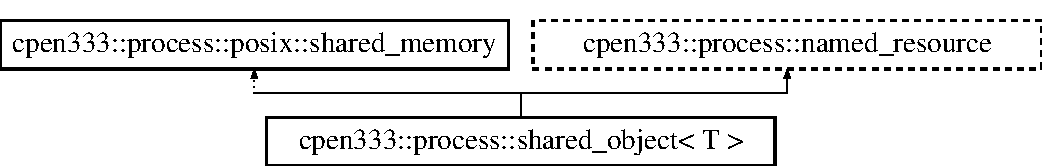
\includegraphics[height=2.000000cm]{classcpen333_1_1process_1_1shared__object}
\end{center}
\end{figure}
\subsection*{Public Member Functions}
\begin{DoxyCompactItemize}
\item 
\hyperlink{classcpen333_1_1process_1_1shared__object_ac8e7c58b5066b058d32e27a7d068f504}{shared\+\_\+object} (const std\+::string \&\hyperlink{classcpen333_1_1process_1_1impl_1_1named__resource__base_ae0c5fbb1843afe863cece4b51c38f807}{name}, bool readonly=false)
\begin{DoxyCompactList}\small\item\em Construct shared memory object. \end{DoxyCompactList}\item 
T \& \hyperlink{classcpen333_1_1process_1_1shared__object_ad1ffd4ad5e13a87f27d9253b816b0b9f}{operator$\ast$} ()
\begin{DoxyCompactList}\small\item\em Get a reference to the internal shared memory object. \end{DoxyCompactList}\item 
T $\ast$ \hyperlink{classcpen333_1_1process_1_1shared__object_ad5a71ce94a79904c4ef85c5a5d1f44f9}{operator-\/$>$} ()
\begin{DoxyCompactList}\small\item\em Get a pointer to the underlying shared memory object. \end{DoxyCompactList}\item 
T $\ast$ \hyperlink{classcpen333_1_1process_1_1shared__object_ac6d38c3ca35cfb102905b6e9dbe4b1ce}{get} ()
\begin{DoxyCompactList}\small\item\em Get a pointer to the underlying shared memory object. \end{DoxyCompactList}\item 
bool \hyperlink{classcpen333_1_1process_1_1shared__object_aa5b43829da5bd2376927e6285745211c}{unlink} ()
\begin{DoxyCompactList}\small\item\em Detaches the name from the named resource. \end{DoxyCompactList}\end{DoxyCompactItemize}
\subsection*{Static Public Member Functions}
\begin{DoxyCompactItemize}
\item 
static bool \hyperlink{classcpen333_1_1process_1_1shared__object_a478c2228031b8471b1e729ce78aabd97}{unlink} (const std\+::string \&\hyperlink{classcpen333_1_1process_1_1impl_1_1named__resource__base_ae0c5fbb1843afe863cece4b51c38f807}{name})
\begin{DoxyCompactList}\small\item\em Unlinks the name without needing to create a resource. \end{DoxyCompactList}\end{DoxyCompactItemize}


\subsection{Detailed Description}
\subsubsection*{template$<$typename T$>$\newline
class cpen333\+::process\+::shared\+\_\+object$<$ T $>$}

Shared memory with a a specific stored type. 

With typed shared memory, the size of the required memory block is automatically computed, and the data pointer is automatically cast to the correct type in \hyperlink{classcpen333_1_1process_1_1shared__object_ac6d38c3ca35cfb102905b6e9dbe4b1ce}{get()}. Member access operators are also overloaded for convenience so the shared object can be used as if it is a direct pointer to the underlying data.


\begin{DoxyTemplParams}{Template Parameters}
{\em T} & data type \\
\hline
\end{DoxyTemplParams}


\subsection{Constructor \& Destructor Documentation}
\mbox{\Hypertarget{classcpen333_1_1process_1_1shared__object_ac8e7c58b5066b058d32e27a7d068f504}\label{classcpen333_1_1process_1_1shared__object_ac8e7c58b5066b058d32e27a7d068f504}} 
\index{cpen333\+::process\+::shared\+\_\+object@{cpen333\+::process\+::shared\+\_\+object}!shared\+\_\+object@{shared\+\_\+object}}
\index{shared\+\_\+object@{shared\+\_\+object}!cpen333\+::process\+::shared\+\_\+object@{cpen333\+::process\+::shared\+\_\+object}}
\subsubsection{\texorpdfstring{shared\+\_\+object()}{shared\_object()}}
{\footnotesize\ttfamily template$<$typename T$>$ \\
\hyperlink{classcpen333_1_1process_1_1shared__object}{cpen333\+::process\+::shared\+\_\+object}$<$ T $>$\+::\hyperlink{classcpen333_1_1process_1_1shared__object}{shared\+\_\+object} (\begin{DoxyParamCaption}\item[{const std\+::string \&}]{name,  }\item[{bool}]{readonly = {\ttfamily false} }\end{DoxyParamCaption})\hspace{0.3cm}{\ttfamily [inline]}}



Construct shared memory object. 


\begin{DoxyParams}{Parameters}
{\em name} & identifier for creating or connecting to an existing inter-\/process \hyperlink{classcpen333_1_1process_1_1shared__object}{shared\+\_\+object} \\
\hline
{\em readonly} & whether to treat the memory as read-\/only or read-\/write \\
\hline
\end{DoxyParams}


\subsection{Member Function Documentation}
\mbox{\Hypertarget{classcpen333_1_1process_1_1shared__object_ac6d38c3ca35cfb102905b6e9dbe4b1ce}\label{classcpen333_1_1process_1_1shared__object_ac6d38c3ca35cfb102905b6e9dbe4b1ce}} 
\index{cpen333\+::process\+::shared\+\_\+object@{cpen333\+::process\+::shared\+\_\+object}!get@{get}}
\index{get@{get}!cpen333\+::process\+::shared\+\_\+object@{cpen333\+::process\+::shared\+\_\+object}}
\subsubsection{\texorpdfstring{get()}{get()}}
{\footnotesize\ttfamily template$<$typename T$>$ \\
T$\ast$ \hyperlink{classcpen333_1_1process_1_1shared__object}{cpen333\+::process\+::shared\+\_\+object}$<$ T $>$\+::get (\begin{DoxyParamCaption}{ }\end{DoxyParamCaption})\hspace{0.3cm}{\ttfamily [inline]}}



Get a pointer to the underlying shared memory object. 

\begin{DoxyReturn}{Returns}
pointer to shared data object 
\end{DoxyReturn}
\mbox{\Hypertarget{classcpen333_1_1process_1_1shared__object_ad1ffd4ad5e13a87f27d9253b816b0b9f}\label{classcpen333_1_1process_1_1shared__object_ad1ffd4ad5e13a87f27d9253b816b0b9f}} 
\index{cpen333\+::process\+::shared\+\_\+object@{cpen333\+::process\+::shared\+\_\+object}!operator$\ast$@{operator$\ast$}}
\index{operator$\ast$@{operator$\ast$}!cpen333\+::process\+::shared\+\_\+object@{cpen333\+::process\+::shared\+\_\+object}}
\subsubsection{\texorpdfstring{operator$\ast$()}{operator*()}}
{\footnotesize\ttfamily template$<$typename T$>$ \\
T\& \hyperlink{classcpen333_1_1process_1_1shared__object}{cpen333\+::process\+::shared\+\_\+object}$<$ T $>$\+::operator$\ast$ (\begin{DoxyParamCaption}{ }\end{DoxyParamCaption})\hspace{0.3cm}{\ttfamily [inline]}}



Get a reference to the internal shared memory object. 

\begin{DoxyReturn}{Returns}
reference to shared data object 
\end{DoxyReturn}
\mbox{\Hypertarget{classcpen333_1_1process_1_1shared__object_ad5a71ce94a79904c4ef85c5a5d1f44f9}\label{classcpen333_1_1process_1_1shared__object_ad5a71ce94a79904c4ef85c5a5d1f44f9}} 
\index{cpen333\+::process\+::shared\+\_\+object@{cpen333\+::process\+::shared\+\_\+object}!operator-\/$>$@{operator-\/$>$}}
\index{operator-\/$>$@{operator-\/$>$}!cpen333\+::process\+::shared\+\_\+object@{cpen333\+::process\+::shared\+\_\+object}}
\subsubsection{\texorpdfstring{operator-\/$>$()}{operator->()}}
{\footnotesize\ttfamily template$<$typename T$>$ \\
T$\ast$ \hyperlink{classcpen333_1_1process_1_1shared__object}{cpen333\+::process\+::shared\+\_\+object}$<$ T $>$\+::operator-\/$>$ (\begin{DoxyParamCaption}{ }\end{DoxyParamCaption})\hspace{0.3cm}{\ttfamily [inline]}}



Get a pointer to the underlying shared memory object. 

\begin{DoxyReturn}{Returns}
pointer to shared data object 
\end{DoxyReturn}
\mbox{\Hypertarget{classcpen333_1_1process_1_1shared__object_aa5b43829da5bd2376927e6285745211c}\label{classcpen333_1_1process_1_1shared__object_aa5b43829da5bd2376927e6285745211c}} 
\index{cpen333\+::process\+::shared\+\_\+object@{cpen333\+::process\+::shared\+\_\+object}!unlink@{unlink}}
\index{unlink@{unlink}!cpen333\+::process\+::shared\+\_\+object@{cpen333\+::process\+::shared\+\_\+object}}
\subsubsection{\texorpdfstring{unlink()}{unlink()}\hspace{0.1cm}{\footnotesize\ttfamily [1/2]}}
{\footnotesize\ttfamily template$<$typename T$>$ \\
bool \hyperlink{classcpen333_1_1process_1_1shared__object}{cpen333\+::process\+::shared\+\_\+object}$<$ T $>$\+::unlink (\begin{DoxyParamCaption}{ }\end{DoxyParamCaption})\hspace{0.3cm}{\ttfamily [inline]}, {\ttfamily [virtual]}}



Detaches the name from the named resource. 

On P\+O\+S\+IX systems, named resources will persist beyond the lifetime of any process that uses them as long as the name has not been unlinked (or until the system is rebooted). Calling {\ttfamily unlink} will detach the name, allowing the resource to be freed once all current users have exited.

\begin{DoxyReturn}{Returns}
{\ttfamily true} if unlink is successful, {\ttfamily false} if unlinking is not supported or if an error has occurred. 
\end{DoxyReturn}


Reimplemented from \hyperlink{classcpen333_1_1process_1_1posix_1_1shared__memory_a3b6d67a41cfaca3712d87958682d8bbe}{cpen333\+::process\+::posix\+::shared\+\_\+memory}.

\mbox{\Hypertarget{classcpen333_1_1process_1_1shared__object_a478c2228031b8471b1e729ce78aabd97}\label{classcpen333_1_1process_1_1shared__object_a478c2228031b8471b1e729ce78aabd97}} 
\index{cpen333\+::process\+::shared\+\_\+object@{cpen333\+::process\+::shared\+\_\+object}!unlink@{unlink}}
\index{unlink@{unlink}!cpen333\+::process\+::shared\+\_\+object@{cpen333\+::process\+::shared\+\_\+object}}
\subsubsection{\texorpdfstring{unlink()}{unlink()}\hspace{0.1cm}{\footnotesize\ttfamily [2/2]}}
{\footnotesize\ttfamily template$<$typename T$>$ \\
static bool \hyperlink{classcpen333_1_1process_1_1shared__object}{cpen333\+::process\+::shared\+\_\+object}$<$ T $>$\+::unlink (\begin{DoxyParamCaption}\item[{const std\+::string \&}]{name }\end{DoxyParamCaption})\hspace{0.3cm}{\ttfamily [inline]}, {\ttfamily [static]}}



Unlinks the name without needing to create a resource. 

Implementers should also provide a static method for unlinking. The purpose is mainly for clean-\/up of existing resources.


\begin{DoxyParams}{Parameters}
{\em name} & desired resource name \\
\hline
\end{DoxyParams}
\begin{DoxyReturn}{Returns}
{\ttfamily true} if unlink successful, {\ttfamily false} if not successful or not supported 
\end{DoxyReturn}


The documentation for this class was generated from the following file\+:\begin{DoxyCompactItemize}
\item 
D\+:/school/teaching/\+C\+P\+E\+N333/workspace/labs/include/cpen333/process/\hyperlink{shared__memory_8h}{shared\+\_\+memory.\+h}\end{DoxyCompactItemize}

\hypertarget{classcpen333_1_1process_1_1shared__timed__mutex}{}\section{cpen333\+:\+:process\+:\+:shared\+\_\+timed\+\_\+mutex Class Reference}
\label{classcpen333_1_1process_1_1shared__timed__mutex}\index{cpen333\+::process\+::shared\+\_\+timed\+\_\+mutex@{cpen333\+::process\+::shared\+\_\+timed\+\_\+mutex}}


An inter-\/process mutual exclusion synchronization primitive allowing for shared access with timeouts.  




{\ttfamily \#include $<$shared\+\_\+mutex.\+h$>$}



\subsection{Detailed Description}
An inter-\/process mutual exclusion synchronization primitive allowing for shared access with timeouts. 

Used to protect access to a resource shared by multiple processes, allowing shared `read\textquotesingle{} access, mirroring std\+::shared\+\_\+timed\+\_\+mutex in c++14. This is an alias to \hyperlink{classcpen333_1_1process_1_1impl_1_1shared__mutex__fair}{cpen333\+::process\+::impl\+::shared\+\_\+mutex\+\_\+fair}. 

The documentation for this class was generated from the following file\+:\begin{DoxyCompactItemize}
\item 
D\+:/school/teaching/\+C\+P\+E\+N333/workspace/labs/include/cpen333/process/\hyperlink{process_2shared__mutex_8h}{shared\+\_\+mutex.\+h}\end{DoxyCompactItemize}

\hypertarget{classcpen333_1_1process_1_1posix_1_1subprocess}{}\section{cpen333\+:\+:process\+:\+:posix\+:\+:subprocess Class Reference}
\label{classcpen333_1_1process_1_1posix_1_1subprocess}\index{cpen333\+::process\+::posix\+::subprocess@{cpen333\+::process\+::posix\+::subprocess}}


A child process.  




{\ttfamily \#include $<$subprocess.\+h$>$}

\subsection*{Public Types}
\begin{DoxyCompactItemize}
\item 
\mbox{\Hypertarget{classcpen333_1_1process_1_1posix_1_1subprocess_a84a93cb8471fd6314591abc6e747fcf4}\label{classcpen333_1_1process_1_1posix_1_1subprocess_a84a93cb8471fd6314591abc6e747fcf4}} 
using \hyperlink{classcpen333_1_1process_1_1posix_1_1subprocess_a84a93cb8471fd6314591abc6e747fcf4}{native\+\_\+handle\+\_\+type} = pid\+\_\+t
\begin{DoxyCompactList}\small\item\em Alias to native handle type, on P\+O\+S\+IX is pid\+\_\+t. \end{DoxyCompactList}\end{DoxyCompactItemize}
\subsection*{Public Member Functions}
\begin{DoxyCompactItemize}
\item 
\hyperlink{classcpen333_1_1process_1_1posix_1_1subprocess_a427822d8d77afa1014a0d10a5f50aa14}{subprocess} (const std\+::vector$<$ std\+::string $>$ \&exec, bool \hyperlink{classcpen333_1_1process_1_1posix_1_1subprocess_a8738add1094b2dda57b9ffb8ec6828c1}{start}=true, bool detached=false)
\begin{DoxyCompactList}\small\item\em Constructs a new subprocess. \end{DoxyCompactList}\item 
\hyperlink{classcpen333_1_1process_1_1posix_1_1subprocess_a5c0d64e12281789fa5ce25f03fa17bd9}{subprocess} (const std\+::string \&cmd, bool \hyperlink{classcpen333_1_1process_1_1posix_1_1subprocess_a8738add1094b2dda57b9ffb8ec6828c1}{start}=true, bool detached=false)
\begin{DoxyCompactList}\small\item\em Constructs a new subprocess from a command string. \end{DoxyCompactList}\item 
bool \hyperlink{classcpen333_1_1process_1_1posix_1_1subprocess_a8738add1094b2dda57b9ffb8ec6828c1}{start} ()
\begin{DoxyCompactList}\small\item\em Starts the subprocess. \end{DoxyCompactList}\item 
bool \hyperlink{classcpen333_1_1process_1_1posix_1_1subprocess_af711962e3b6649476bd8cbbd6c59ea8b}{join} ()
\begin{DoxyCompactList}\small\item\em Waits for the subprocess to complete execution. \end{DoxyCompactList}\item 
bool \hyperlink{classcpen333_1_1process_1_1posix_1_1subprocess_a8928b9937577c0ec288318b2176156a0}{wait} ()
\begin{DoxyCompactList}\small\item\em Waits for the subprocess to complete execution. \end{DoxyCompactList}\item 
{\footnotesize template$<$typename Rep , typename Period $>$ }\\bool \hyperlink{classcpen333_1_1process_1_1posix_1_1subprocess_a1543488d24eaf0f819e81f31d9d388cb}{wait\+\_\+for} (const std\+::chrono\+::duration$<$ Rep, Period $>$ \&duration)
\begin{DoxyCompactList}\small\item\em Waits for the process to terminate up to a maximum amount of time. \end{DoxyCompactList}\item 
{\footnotesize template$<$class Clock , class Duration $>$ }\\bool \hyperlink{classcpen333_1_1process_1_1posix_1_1subprocess_a10ea54174a30dd26c0d1ff289b88cd42}{wait\+\_\+until} (const std\+::chrono\+::time\+\_\+point$<$ Clock, Duration $>$ \&timeout\+\_\+time)
\begin{DoxyCompactList}\small\item\em Waits for the process to terminate up to a maximum absolute time. \end{DoxyCompactList}\item 
bool \hyperlink{classcpen333_1_1process_1_1posix_1_1subprocess_aabc5ed98ead25bc40663e586a83e62bb}{terminated} ()
\begin{DoxyCompactList}\small\item\em Checks if the process has already been terminated. \end{DoxyCompactList}\item 
bool \hyperlink{classcpen333_1_1process_1_1posix_1_1subprocess_aee0a935ed7052a7622872345bd148ca1}{terminate} ()
\begin{DoxyCompactList}\small\item\em Force the process to terminate. \end{DoxyCompactList}\end{DoxyCompactItemize}


\subsection{Detailed Description}
A child process. 

Allows launching of a child process, with environment inherited from the current process. 

\subsection{Constructor \& Destructor Documentation}
\mbox{\Hypertarget{classcpen333_1_1process_1_1posix_1_1subprocess_a427822d8d77afa1014a0d10a5f50aa14}\label{classcpen333_1_1process_1_1posix_1_1subprocess_a427822d8d77afa1014a0d10a5f50aa14}} 
\index{cpen333\+::process\+::posix\+::subprocess@{cpen333\+::process\+::posix\+::subprocess}!subprocess@{subprocess}}
\index{subprocess@{subprocess}!cpen333\+::process\+::posix\+::subprocess@{cpen333\+::process\+::posix\+::subprocess}}
\subsubsection{\texorpdfstring{subprocess()}{subprocess()}\hspace{0.1cm}{\footnotesize\ttfamily [1/2]}}
{\footnotesize\ttfamily cpen333\+::process\+::posix\+::subprocess\+::subprocess (\begin{DoxyParamCaption}\item[{const std\+::vector$<$ std\+::string $>$ \&}]{exec,  }\item[{bool}]{start = {\ttfamily true},  }\item[{bool}]{detached = {\ttfamily false} }\end{DoxyParamCaption})\hspace{0.3cm}{\ttfamily [inline]}}



Constructs a new subprocess. 

The new process will run the command exec\mbox{[}0\mbox{]} with argv parameters \{exec\mbox{[}1\mbox{]}, exec\mbox{[}2\mbox{]}, ...\}. A detached child process will run in a separate thread, concurrently with the parent process. If not detached, the parent will wait for a running child to complete.


\begin{DoxyParams}{Parameters}
{\em exec} & command and arguments to execute \\
\hline
{\em start} & whether to start the subprocess immediately \\
\hline
{\em detached} & run the subprocess in `detached\textquotesingle{} mode \\
\hline
\end{DoxyParams}
\mbox{\Hypertarget{classcpen333_1_1process_1_1posix_1_1subprocess_a5c0d64e12281789fa5ce25f03fa17bd9}\label{classcpen333_1_1process_1_1posix_1_1subprocess_a5c0d64e12281789fa5ce25f03fa17bd9}} 
\index{cpen333\+::process\+::posix\+::subprocess@{cpen333\+::process\+::posix\+::subprocess}!subprocess@{subprocess}}
\index{subprocess@{subprocess}!cpen333\+::process\+::posix\+::subprocess@{cpen333\+::process\+::posix\+::subprocess}}
\subsubsection{\texorpdfstring{subprocess()}{subprocess()}\hspace{0.1cm}{\footnotesize\ttfamily [2/2]}}
{\footnotesize\ttfamily cpen333\+::process\+::posix\+::subprocess\+::subprocess (\begin{DoxyParamCaption}\item[{const std\+::string \&}]{cmd,  }\item[{bool}]{start = {\ttfamily true},  }\item[{bool}]{detached = {\ttfamily false} }\end{DoxyParamCaption})\hspace{0.3cm}{\ttfamily [inline]}}



Constructs a new subprocess from a command string. 

The new process will run the command cmd with argv parameters parsed from the string. A detached child process will run in a separate thread, concurrently with the parent process. If not detached, the parent will wait for a running child to complete.

N\+O\+TE\+: this is much less safe than subprocess(const std\+::vector$<$std\+::string$>$,bool,bool), which should be preferred when there are multiple arguments or if string parsing might be ambiguous


\begin{DoxyParams}{Parameters}
{\em cmd} & command, potentially containing arguments to parse \\
\hline
{\em start} & whether to start the subprocess immediately \\
\hline
{\em detached} & run the process in `detached\textquotesingle{} mode \\
\hline
\end{DoxyParams}


\subsection{Member Function Documentation}
\mbox{\Hypertarget{classcpen333_1_1process_1_1posix_1_1subprocess_af711962e3b6649476bd8cbbd6c59ea8b}\label{classcpen333_1_1process_1_1posix_1_1subprocess_af711962e3b6649476bd8cbbd6c59ea8b}} 
\index{cpen333\+::process\+::posix\+::subprocess@{cpen333\+::process\+::posix\+::subprocess}!join@{join}}
\index{join@{join}!cpen333\+::process\+::posix\+::subprocess@{cpen333\+::process\+::posix\+::subprocess}}
\subsubsection{\texorpdfstring{join()}{join()}}
{\footnotesize\ttfamily bool cpen333\+::process\+::posix\+::subprocess\+::join (\begin{DoxyParamCaption}{ }\end{DoxyParamCaption})\hspace{0.3cm}{\ttfamily [inline]}}



Waits for the subprocess to complete execution. 

\begin{DoxyReturn}{Returns}
true if joined successfully, false if the process has already been joined or if an error occurs 
\end{DoxyReturn}
\mbox{\Hypertarget{classcpen333_1_1process_1_1posix_1_1subprocess_a8738add1094b2dda57b9ffb8ec6828c1}\label{classcpen333_1_1process_1_1posix_1_1subprocess_a8738add1094b2dda57b9ffb8ec6828c1}} 
\index{cpen333\+::process\+::posix\+::subprocess@{cpen333\+::process\+::posix\+::subprocess}!start@{start}}
\index{start@{start}!cpen333\+::process\+::posix\+::subprocess@{cpen333\+::process\+::posix\+::subprocess}}
\subsubsection{\texorpdfstring{start()}{start()}}
{\footnotesize\ttfamily bool cpen333\+::process\+::posix\+::subprocess\+::start (\begin{DoxyParamCaption}{ }\end{DoxyParamCaption})\hspace{0.3cm}{\ttfamily [inline]}}



Starts the subprocess. 

\begin{DoxyReturn}{Returns}
true if started, false if process already started or an error occurs 
\end{DoxyReturn}
\mbox{\Hypertarget{classcpen333_1_1process_1_1posix_1_1subprocess_aee0a935ed7052a7622872345bd148ca1}\label{classcpen333_1_1process_1_1posix_1_1subprocess_aee0a935ed7052a7622872345bd148ca1}} 
\index{cpen333\+::process\+::posix\+::subprocess@{cpen333\+::process\+::posix\+::subprocess}!terminate@{terminate}}
\index{terminate@{terminate}!cpen333\+::process\+::posix\+::subprocess@{cpen333\+::process\+::posix\+::subprocess}}
\subsubsection{\texorpdfstring{terminate()}{terminate()}}
{\footnotesize\ttfamily bool cpen333\+::process\+::posix\+::subprocess\+::terminate (\begin{DoxyParamCaption}{ }\end{DoxyParamCaption})\hspace{0.3cm}{\ttfamily [inline]}}



Force the process to terminate. 

\begin{DoxyReturn}{Returns}
true if successful 
\end{DoxyReturn}
\mbox{\Hypertarget{classcpen333_1_1process_1_1posix_1_1subprocess_aabc5ed98ead25bc40663e586a83e62bb}\label{classcpen333_1_1process_1_1posix_1_1subprocess_aabc5ed98ead25bc40663e586a83e62bb}} 
\index{cpen333\+::process\+::posix\+::subprocess@{cpen333\+::process\+::posix\+::subprocess}!terminated@{terminated}}
\index{terminated@{terminated}!cpen333\+::process\+::posix\+::subprocess@{cpen333\+::process\+::posix\+::subprocess}}
\subsubsection{\texorpdfstring{terminated()}{terminated()}}
{\footnotesize\ttfamily bool cpen333\+::process\+::posix\+::subprocess\+::terminated (\begin{DoxyParamCaption}{ }\end{DoxyParamCaption})\hspace{0.3cm}{\ttfamily [inline]}}



Checks if the process has already been terminated. 

\begin{DoxyReturn}{Returns}

\end{DoxyReturn}
\mbox{\Hypertarget{classcpen333_1_1process_1_1posix_1_1subprocess_a8928b9937577c0ec288318b2176156a0}\label{classcpen333_1_1process_1_1posix_1_1subprocess_a8928b9937577c0ec288318b2176156a0}} 
\index{cpen333\+::process\+::posix\+::subprocess@{cpen333\+::process\+::posix\+::subprocess}!wait@{wait}}
\index{wait@{wait}!cpen333\+::process\+::posix\+::subprocess@{cpen333\+::process\+::posix\+::subprocess}}
\subsubsection{\texorpdfstring{wait()}{wait()}}
{\footnotesize\ttfamily bool cpen333\+::process\+::posix\+::subprocess\+::wait (\begin{DoxyParamCaption}{ }\end{DoxyParamCaption})\hspace{0.3cm}{\ttfamily [inline]}}



Waits for the subprocess to complete execution. 

Similar to \hyperlink{classcpen333_1_1process_1_1posix_1_1subprocess_af711962e3b6649476bd8cbbd6c59ea8b}{join()}, but will return true if the process has already been joined

\begin{DoxyReturn}{Returns}
true if process terminates or is already terminated 
\end{DoxyReturn}
\mbox{\Hypertarget{classcpen333_1_1process_1_1posix_1_1subprocess_a1543488d24eaf0f819e81f31d9d388cb}\label{classcpen333_1_1process_1_1posix_1_1subprocess_a1543488d24eaf0f819e81f31d9d388cb}} 
\index{cpen333\+::process\+::posix\+::subprocess@{cpen333\+::process\+::posix\+::subprocess}!wait\+\_\+for@{wait\+\_\+for}}
\index{wait\+\_\+for@{wait\+\_\+for}!cpen333\+::process\+::posix\+::subprocess@{cpen333\+::process\+::posix\+::subprocess}}
\subsubsection{\texorpdfstring{wait\+\_\+for()}{wait\_for()}}
{\footnotesize\ttfamily template$<$typename Rep , typename Period $>$ \\
bool cpen333\+::process\+::posix\+::subprocess\+::wait\+\_\+for (\begin{DoxyParamCaption}\item[{const std\+::chrono\+::duration$<$ Rep, Period $>$ \&}]{duration }\end{DoxyParamCaption})\hspace{0.3cm}{\ttfamily [inline]}}



Waits for the process to terminate up to a maximum amount of time. 


\begin{DoxyTemplParams}{Template Parameters}
{\em Rep} & duration representation \\
\hline
{\em Period} & duration tick period \\
\hline
\end{DoxyTemplParams}

\begin{DoxyParams}{Parameters}
{\em duration} & maximum relative time to wait for \\
\hline
\end{DoxyParams}
\begin{DoxyReturn}{Returns}
true if process terminates or is already terminated 
\end{DoxyReturn}
\mbox{\Hypertarget{classcpen333_1_1process_1_1posix_1_1subprocess_a10ea54174a30dd26c0d1ff289b88cd42}\label{classcpen333_1_1process_1_1posix_1_1subprocess_a10ea54174a30dd26c0d1ff289b88cd42}} 
\index{cpen333\+::process\+::posix\+::subprocess@{cpen333\+::process\+::posix\+::subprocess}!wait\+\_\+until@{wait\+\_\+until}}
\index{wait\+\_\+until@{wait\+\_\+until}!cpen333\+::process\+::posix\+::subprocess@{cpen333\+::process\+::posix\+::subprocess}}
\subsubsection{\texorpdfstring{wait\+\_\+until()}{wait\_until()}}
{\footnotesize\ttfamily template$<$class Clock , class Duration $>$ \\
bool cpen333\+::process\+::posix\+::subprocess\+::wait\+\_\+until (\begin{DoxyParamCaption}\item[{const std\+::chrono\+::time\+\_\+point$<$ Clock, Duration $>$ \&}]{timeout\+\_\+time }\end{DoxyParamCaption})\hspace{0.3cm}{\ttfamily [inline]}}



Waits for the process to terminate up to a maximum absolute time. 


\begin{DoxyTemplParams}{Template Parameters}
{\em Clock} & timeout clock type \\
\hline
{\em Duration} & timeout clock duration type \\
\hline
\end{DoxyTemplParams}

\begin{DoxyParams}{Parameters}
{\em timeout\+\_\+time} & absolute timeout time \\
\hline
\end{DoxyParams}
\begin{DoxyReturn}{Returns}
true if process terminates or is already terminated 
\end{DoxyReturn}


The documentation for this class was generated from the following file\+:\begin{DoxyCompactItemize}
\item 
D\+:/school/teaching/\+C\+P\+E\+N333/workspace/library/include/cpen333/process/impl/posix/\hyperlink{impl_2posix_2subprocess_8h}{subprocess.\+h}\end{DoxyCompactItemize}

\hypertarget{classcpen333_1_1process_1_1subprocess}{}\section{cpen333\+:\+:process\+:\+:subprocess Class Reference}
\label{classcpen333_1_1process_1_1subprocess}\index{cpen333\+::process\+::subprocess@{cpen333\+::process\+::subprocess}}


A child process implementation.  




{\ttfamily \#include $<$subprocess.\+h$>$}



\subsection{Detailed Description}
A child process implementation. 

Used to create and run a child process. This is an alias to either \hyperlink{classcpen333_1_1process_1_1posix_1_1subprocess}{cpen333\+::process\+::posix\+::subprocess} or \hyperlink{classcpen333_1_1process_1_1windows_1_1subprocess}{cpen333\+::process\+::windows\+::subprocess} depending on your platform. 

The documentation for this class was generated from the following file\+:\begin{DoxyCompactItemize}
\item 
D\+:/school/teaching/\+C\+P\+E\+N333/workspace/library/include/cpen333/process/\hyperlink{subprocess_8h}{subprocess.\+h}\end{DoxyCompactItemize}

\hypertarget{classcpen333_1_1process_1_1windows_1_1subprocess}{}\section{cpen333\+:\+:process\+:\+:windows\+:\+:subprocess Class Reference}
\label{classcpen333_1_1process_1_1windows_1_1subprocess}\index{cpen333\+::process\+::windows\+::subprocess@{cpen333\+::process\+::windows\+::subprocess}}


A child process.  




{\ttfamily \#include $<$subprocess.\+h$>$}

\subsection*{Public Types}
\begin{DoxyCompactItemize}
\item 
\mbox{\Hypertarget{classcpen333_1_1process_1_1windows_1_1subprocess_a579616d8fd1401a85aae1046412f451d}\label{classcpen333_1_1process_1_1windows_1_1subprocess_a579616d8fd1401a85aae1046412f451d}} 
using \hyperlink{classcpen333_1_1process_1_1windows_1_1subprocess_a579616d8fd1401a85aae1046412f451d}{native\+\_\+handle\+\_\+type} = P\+R\+O\+C\+E\+S\+S\+\_\+\+I\+N\+F\+O\+R\+M\+A\+T\+I\+ON
\begin{DoxyCompactList}\small\item\em Alias to native handle type, on Windows is a P\+R\+O\+C\+E\+S\+S\+\_\+\+I\+N\+F\+O\+R\+M\+A\+T\+I\+ON structure. \end{DoxyCompactList}\end{DoxyCompactItemize}
\subsection*{Public Member Functions}
\begin{DoxyCompactItemize}
\item 
\hyperlink{classcpen333_1_1process_1_1windows_1_1subprocess_ab927ab6d2b499cb7079bc2dedbd670ff}{subprocess} (const std\+::vector$<$ std\+::string $>$ \&exec, bool \hyperlink{classcpen333_1_1process_1_1windows_1_1subprocess_ad6fddf2c148cefff9753dafaeb35d1a3}{start}=true, bool detached=false)
\begin{DoxyCompactList}\small\item\em Constructs a new subprocess. \end{DoxyCompactList}\item 
bool \hyperlink{classcpen333_1_1process_1_1windows_1_1subprocess_ad6fddf2c148cefff9753dafaeb35d1a3}{start} ()
\begin{DoxyCompactList}\small\item\em Starts the subprocess. \end{DoxyCompactList}\item 
bool \hyperlink{classcpen333_1_1process_1_1windows_1_1subprocess_a973a466ad1f7299d1511e4a0628bc3f4}{join} ()
\begin{DoxyCompactList}\small\item\em Waits for the subprocess to complete execution. \end{DoxyCompactList}\item 
bool \hyperlink{classcpen333_1_1process_1_1windows_1_1subprocess_a54fe40167d1bf23bce4195c5aa34ec5f}{wait} ()
\begin{DoxyCompactList}\small\item\em Waits for the subprocess to complete execution. \end{DoxyCompactList}\item 
{\footnotesize template$<$typename Rep , typename Period $>$ }\\bool \hyperlink{classcpen333_1_1process_1_1windows_1_1subprocess_aed7bf88b47dfa88ba8c97d6dbc94c124}{wait\+\_\+for} (const std\+::chrono\+::duration$<$ Rep, Period $>$ \&duration)
\begin{DoxyCompactList}\small\item\em Waits for the process to terminate up to a maximum amount of time. \end{DoxyCompactList}\item 
{\footnotesize template$<$class Clock , class Duration $>$ }\\bool \hyperlink{classcpen333_1_1process_1_1windows_1_1subprocess_a228f617ee1ef52374041d6dd094105ba}{wait\+\_\+until} (const std\+::chrono\+::time\+\_\+point$<$ Clock, Duration $>$ \&timeout\+\_\+time)
\begin{DoxyCompactList}\small\item\em Waits for the process to terminate up to a maximum absolute time. \end{DoxyCompactList}\item 
bool \hyperlink{classcpen333_1_1process_1_1windows_1_1subprocess_a7fc3a589bdd4cde9adb09fc3debf9bc9}{terminated} ()
\begin{DoxyCompactList}\small\item\em Checks if the process has already been terminated. \end{DoxyCompactList}\end{DoxyCompactItemize}


\subsection{Detailed Description}
A child process. 

Allows launching of a child process, with environment inherited from the current process. 

\subsection{Constructor \& Destructor Documentation}
\mbox{\Hypertarget{classcpen333_1_1process_1_1windows_1_1subprocess_ab927ab6d2b499cb7079bc2dedbd670ff}\label{classcpen333_1_1process_1_1windows_1_1subprocess_ab927ab6d2b499cb7079bc2dedbd670ff}} 
\index{cpen333\+::process\+::windows\+::subprocess@{cpen333\+::process\+::windows\+::subprocess}!subprocess@{subprocess}}
\index{subprocess@{subprocess}!cpen333\+::process\+::windows\+::subprocess@{cpen333\+::process\+::windows\+::subprocess}}
\subsubsection{\texorpdfstring{subprocess()}{subprocess()}}
{\footnotesize\ttfamily cpen333\+::process\+::windows\+::subprocess\+::subprocess (\begin{DoxyParamCaption}\item[{const std\+::vector$<$ std\+::string $>$ \&}]{exec,  }\item[{bool}]{start = {\ttfamily true},  }\item[{bool}]{detached = {\ttfamily false} }\end{DoxyParamCaption})\hspace{0.3cm}{\ttfamily [inline]}}



Constructs a new subprocess. 

The new process will run the command exec\mbox{[}0\mbox{]} with argv parameters \{exec\mbox{[}1\mbox{]}, exec\mbox{[}2\mbox{]}, ...\}. A detached child process will run in a separate thread, (and on Windows, a separate window) concurrently with the parent process. If not detached, the parent will wait for a running child to complete.


\begin{DoxyParams}{Parameters}
{\em exec} & command and arguments to execute \\
\hline
{\em start} & whether to start the subprocess immediately \\
\hline
{\em detached} & run the subprocess in `detached\textquotesingle{} mode \\
\hline
\end{DoxyParams}


\subsection{Member Function Documentation}
\mbox{\Hypertarget{classcpen333_1_1process_1_1windows_1_1subprocess_a973a466ad1f7299d1511e4a0628bc3f4}\label{classcpen333_1_1process_1_1windows_1_1subprocess_a973a466ad1f7299d1511e4a0628bc3f4}} 
\index{cpen333\+::process\+::windows\+::subprocess@{cpen333\+::process\+::windows\+::subprocess}!join@{join}}
\index{join@{join}!cpen333\+::process\+::windows\+::subprocess@{cpen333\+::process\+::windows\+::subprocess}}
\subsubsection{\texorpdfstring{join()}{join()}}
{\footnotesize\ttfamily bool cpen333\+::process\+::windows\+::subprocess\+::join (\begin{DoxyParamCaption}{ }\end{DoxyParamCaption})\hspace{0.3cm}{\ttfamily [inline]}}



Waits for the subprocess to complete execution. 

\begin{DoxyReturn}{Returns}
true if joined successfully, false if the process has already been joined or if an error occurs 
\end{DoxyReturn}
\mbox{\Hypertarget{classcpen333_1_1process_1_1windows_1_1subprocess_ad6fddf2c148cefff9753dafaeb35d1a3}\label{classcpen333_1_1process_1_1windows_1_1subprocess_ad6fddf2c148cefff9753dafaeb35d1a3}} 
\index{cpen333\+::process\+::windows\+::subprocess@{cpen333\+::process\+::windows\+::subprocess}!start@{start}}
\index{start@{start}!cpen333\+::process\+::windows\+::subprocess@{cpen333\+::process\+::windows\+::subprocess}}
\subsubsection{\texorpdfstring{start()}{start()}}
{\footnotesize\ttfamily bool cpen333\+::process\+::windows\+::subprocess\+::start (\begin{DoxyParamCaption}{ }\end{DoxyParamCaption})\hspace{0.3cm}{\ttfamily [inline]}}



Starts the subprocess. 

\begin{DoxyReturn}{Returns}
true if started, false if process already started or an error occurs 
\end{DoxyReturn}
\mbox{\Hypertarget{classcpen333_1_1process_1_1windows_1_1subprocess_a7fc3a589bdd4cde9adb09fc3debf9bc9}\label{classcpen333_1_1process_1_1windows_1_1subprocess_a7fc3a589bdd4cde9adb09fc3debf9bc9}} 
\index{cpen333\+::process\+::windows\+::subprocess@{cpen333\+::process\+::windows\+::subprocess}!terminated@{terminated}}
\index{terminated@{terminated}!cpen333\+::process\+::windows\+::subprocess@{cpen333\+::process\+::windows\+::subprocess}}
\subsubsection{\texorpdfstring{terminated()}{terminated()}}
{\footnotesize\ttfamily bool cpen333\+::process\+::windows\+::subprocess\+::terminated (\begin{DoxyParamCaption}{ }\end{DoxyParamCaption})\hspace{0.3cm}{\ttfamily [inline]}}



Checks if the process has already been terminated. 

\begin{DoxyReturn}{Returns}

\end{DoxyReturn}
\mbox{\Hypertarget{classcpen333_1_1process_1_1windows_1_1subprocess_a54fe40167d1bf23bce4195c5aa34ec5f}\label{classcpen333_1_1process_1_1windows_1_1subprocess_a54fe40167d1bf23bce4195c5aa34ec5f}} 
\index{cpen333\+::process\+::windows\+::subprocess@{cpen333\+::process\+::windows\+::subprocess}!wait@{wait}}
\index{wait@{wait}!cpen333\+::process\+::windows\+::subprocess@{cpen333\+::process\+::windows\+::subprocess}}
\subsubsection{\texorpdfstring{wait()}{wait()}}
{\footnotesize\ttfamily bool cpen333\+::process\+::windows\+::subprocess\+::wait (\begin{DoxyParamCaption}{ }\end{DoxyParamCaption})\hspace{0.3cm}{\ttfamily [inline]}}



Waits for the subprocess to complete execution. 

Similar to \hyperlink{classcpen333_1_1process_1_1windows_1_1subprocess_a973a466ad1f7299d1511e4a0628bc3f4}{join()}, but will return true if the process has already been joined

\begin{DoxyReturn}{Returns}
true if process terminates or is already terminated 
\end{DoxyReturn}
\mbox{\Hypertarget{classcpen333_1_1process_1_1windows_1_1subprocess_aed7bf88b47dfa88ba8c97d6dbc94c124}\label{classcpen333_1_1process_1_1windows_1_1subprocess_aed7bf88b47dfa88ba8c97d6dbc94c124}} 
\index{cpen333\+::process\+::windows\+::subprocess@{cpen333\+::process\+::windows\+::subprocess}!wait\+\_\+for@{wait\+\_\+for}}
\index{wait\+\_\+for@{wait\+\_\+for}!cpen333\+::process\+::windows\+::subprocess@{cpen333\+::process\+::windows\+::subprocess}}
\subsubsection{\texorpdfstring{wait\+\_\+for()}{wait\_for()}}
{\footnotesize\ttfamily template$<$typename Rep , typename Period $>$ \\
bool cpen333\+::process\+::windows\+::subprocess\+::wait\+\_\+for (\begin{DoxyParamCaption}\item[{const std\+::chrono\+::duration$<$ Rep, Period $>$ \&}]{duration }\end{DoxyParamCaption})\hspace{0.3cm}{\ttfamily [inline]}}



Waits for the process to terminate up to a maximum amount of time. 


\begin{DoxyTemplParams}{Template Parameters}
{\em Rep} & duration representation \\
\hline
{\em Period} & duration tick period \\
\hline
\end{DoxyTemplParams}

\begin{DoxyParams}{Parameters}
{\em duration} & maximum relative time to wait for \\
\hline
\end{DoxyParams}
\begin{DoxyReturn}{Returns}
true if process terminates or is already terminated 
\end{DoxyReturn}
\mbox{\Hypertarget{classcpen333_1_1process_1_1windows_1_1subprocess_a228f617ee1ef52374041d6dd094105ba}\label{classcpen333_1_1process_1_1windows_1_1subprocess_a228f617ee1ef52374041d6dd094105ba}} 
\index{cpen333\+::process\+::windows\+::subprocess@{cpen333\+::process\+::windows\+::subprocess}!wait\+\_\+until@{wait\+\_\+until}}
\index{wait\+\_\+until@{wait\+\_\+until}!cpen333\+::process\+::windows\+::subprocess@{cpen333\+::process\+::windows\+::subprocess}}
\subsubsection{\texorpdfstring{wait\+\_\+until()}{wait\_until()}}
{\footnotesize\ttfamily template$<$class Clock , class Duration $>$ \\
bool cpen333\+::process\+::windows\+::subprocess\+::wait\+\_\+until (\begin{DoxyParamCaption}\item[{const std\+::chrono\+::time\+\_\+point$<$ Clock, Duration $>$ \&}]{timeout\+\_\+time }\end{DoxyParamCaption})\hspace{0.3cm}{\ttfamily [inline]}}



Waits for the process to terminate up to a maximum absolute time. 


\begin{DoxyTemplParams}{Template Parameters}
{\em Clock} & timeout clock type \\
\hline
{\em Duration} & timeout clock duration type \\
\hline
\end{DoxyTemplParams}

\begin{DoxyParams}{Parameters}
{\em timeout\+\_\+time} & absolute timeout time \\
\hline
\end{DoxyParams}
\begin{DoxyReturn}{Returns}
true if process terminates or is already terminated 
\end{DoxyReturn}


The documentation for this class was generated from the following file\+:\begin{DoxyCompactItemize}
\item 
D\+:/school/teaching/\+C\+P\+E\+N333/workspace/labs/include/cpen333/process/impl/windows/\hyperlink{impl_2windows_2subprocess_8h}{subprocess.\+h}\end{DoxyCompactItemize}

\hypertarget{classcpen333_1_1thread_1_1thread__object}{}\section{cpen333\+:\+:thread\+:\+:thread\+\_\+object Class Reference}
\label{classcpen333_1_1thread_1_1thread__object}\index{cpen333\+::thread\+::thread\+\_\+object@{cpen333\+::thread\+::thread\+\_\+object}}


Base object-\/oriented thread object.  




{\ttfamily \#include $<$thread\+\_\+object.\+h$>$}

\subsection*{Public Member Functions}
\begin{DoxyCompactItemize}
\item 
\mbox{\Hypertarget{classcpen333_1_1thread_1_1thread__object_a1e15fda903a0e1bbc0c06fc7d870d0d9}\label{classcpen333_1_1thread_1_1thread__object_a1e15fda903a0e1bbc0c06fc7d870d0d9}} 
\hyperlink{classcpen333_1_1thread_1_1thread__object_a1e15fda903a0e1bbc0c06fc7d870d0d9}{thread\+\_\+object} ()
\begin{DoxyCompactList}\small\item\em Constructs the thread base. \end{DoxyCompactList}\item 
\mbox{\Hypertarget{classcpen333_1_1thread_1_1thread__object_addcca372aa82c04d454ade7fd60d1e75}\label{classcpen333_1_1thread_1_1thread__object_addcca372aa82c04d454ade7fd60d1e75}} 
\hyperlink{classcpen333_1_1thread_1_1thread__object_addcca372aa82c04d454ade7fd60d1e75}{$\sim$thread\+\_\+object} ()
\begin{DoxyCompactList}\small\item\em Destructor, frees the thread. \end{DoxyCompactList}\item 
void \hyperlink{classcpen333_1_1thread_1_1thread__object_ae4484909a3f4418c0c0db318d615bde1}{start} ()
\begin{DoxyCompactList}\small\item\em Start thread execution. \end{DoxyCompactList}\item 
int \hyperlink{classcpen333_1_1thread_1_1thread__object_ac7334918eabfcf855cec00ed2a68a039}{join} ()
\begin{DoxyCompactList}\small\item\em Waits for thread to finish executing. \end{DoxyCompactList}\item 
\mbox{\Hypertarget{classcpen333_1_1thread_1_1thread__object_a6e6fd163c5f5f72dcd6385a74ad316b6}\label{classcpen333_1_1thread_1_1thread__object_a6e6fd163c5f5f72dcd6385a74ad316b6}} 
void \hyperlink{classcpen333_1_1thread_1_1thread__object_a6e6fd163c5f5f72dcd6385a74ad316b6}{detach} ()
\begin{DoxyCompactList}\small\item\em Allows the thread to execute independently from the thread\textquotesingle{}s handle. \end{DoxyCompactList}\item 
bool \hyperlink{classcpen333_1_1thread_1_1thread__object_a374e31ea56accc37a3468012a411da5d}{joinable} ()
\begin{DoxyCompactList}\small\item\em Checks whether the thread is joinable. \end{DoxyCompactList}\end{DoxyCompactItemize}
\subsection*{Protected Member Functions}
\begin{DoxyCompactItemize}
\item 
virtual int \hyperlink{classcpen333_1_1thread_1_1thread__object_adbd74f6f7461d90a1c12e8078aa5f3af}{main} ()=0
\begin{DoxyCompactList}\small\item\em Main execution method of thread. \end{DoxyCompactList}\end{DoxyCompactItemize}


\subsection{Detailed Description}
Base object-\/oriented thread object. 

Virtual object with a \hyperlink{classcpen333_1_1thread_1_1thread__object_adbd74f6f7461d90a1c12e8078aa5f3af}{main()} method that must be overridden which will execute once the thread is started. Also has functionality to return the returned value of \hyperlink{classcpen333_1_1thread_1_1thread__object_adbd74f6f7461d90a1c12e8078aa5f3af}{main()}.

The thread is N\+OT started automatically (nor should it be due to memory access concerns). 

\subsection{Member Function Documentation}
\mbox{\Hypertarget{classcpen333_1_1thread_1_1thread__object_ac7334918eabfcf855cec00ed2a68a039}\label{classcpen333_1_1thread_1_1thread__object_ac7334918eabfcf855cec00ed2a68a039}} 
\index{cpen333\+::thread\+::thread\+\_\+object@{cpen333\+::thread\+::thread\+\_\+object}!join@{join}}
\index{join@{join}!cpen333\+::thread\+::thread\+\_\+object@{cpen333\+::thread\+::thread\+\_\+object}}
\subsubsection{\texorpdfstring{join()}{join()}}
{\footnotesize\ttfamily int cpen333\+::thread\+::thread\+\_\+object\+::join (\begin{DoxyParamCaption}{ }\end{DoxyParamCaption})\hspace{0.3cm}{\ttfamily [inline]}}



Waits for thread to finish executing. 

If thread hasn\textquotesingle{}t been started yet, then it is started here.

\begin{DoxyReturn}{Returns}
the result of \hyperlink{classcpen333_1_1thread_1_1thread__object_adbd74f6f7461d90a1c12e8078aa5f3af}{main()} 
\end{DoxyReturn}
\mbox{\Hypertarget{classcpen333_1_1thread_1_1thread__object_a374e31ea56accc37a3468012a411da5d}\label{classcpen333_1_1thread_1_1thread__object_a374e31ea56accc37a3468012a411da5d}} 
\index{cpen333\+::thread\+::thread\+\_\+object@{cpen333\+::thread\+::thread\+\_\+object}!joinable@{joinable}}
\index{joinable@{joinable}!cpen333\+::thread\+::thread\+\_\+object@{cpen333\+::thread\+::thread\+\_\+object}}
\subsubsection{\texorpdfstring{joinable()}{joinable()}}
{\footnotesize\ttfamily bool cpen333\+::thread\+::thread\+\_\+object\+::joinable (\begin{DoxyParamCaption}{ }\end{DoxyParamCaption})\hspace{0.3cm}{\ttfamily [inline]}}



Checks whether the thread is joinable. 

i.\+e. the thread has not already been joined, and is not detached

\begin{DoxyReturn}{Returns}
true if thread is running and joinable, false otherwise 
\end{DoxyReturn}
\mbox{\Hypertarget{classcpen333_1_1thread_1_1thread__object_adbd74f6f7461d90a1c12e8078aa5f3af}\label{classcpen333_1_1thread_1_1thread__object_adbd74f6f7461d90a1c12e8078aa5f3af}} 
\index{cpen333\+::thread\+::thread\+\_\+object@{cpen333\+::thread\+::thread\+\_\+object}!main@{main}}
\index{main@{main}!cpen333\+::thread\+::thread\+\_\+object@{cpen333\+::thread\+::thread\+\_\+object}}
\subsubsection{\texorpdfstring{main()}{main()}}
{\footnotesize\ttfamily virtual int cpen333\+::thread\+::thread\+\_\+object\+::main (\begin{DoxyParamCaption}{ }\end{DoxyParamCaption})\hspace{0.3cm}{\ttfamily [protected]}, {\ttfamily [pure virtual]}}



Main execution method of thread. 

\begin{DoxyReturn}{Returns}
main return value 
\end{DoxyReturn}
\mbox{\Hypertarget{classcpen333_1_1thread_1_1thread__object_ae4484909a3f4418c0c0db318d615bde1}\label{classcpen333_1_1thread_1_1thread__object_ae4484909a3f4418c0c0db318d615bde1}} 
\index{cpen333\+::thread\+::thread\+\_\+object@{cpen333\+::thread\+::thread\+\_\+object}!start@{start}}
\index{start@{start}!cpen333\+::thread\+::thread\+\_\+object@{cpen333\+::thread\+::thread\+\_\+object}}
\subsubsection{\texorpdfstring{start()}{start()}}
{\footnotesize\ttfamily void cpen333\+::thread\+::thread\+\_\+object\+::start (\begin{DoxyParamCaption}{ }\end{DoxyParamCaption})\hspace{0.3cm}{\ttfamily [inline]}}



Start thread execution. 

Runs the \hyperlink{classcpen333_1_1thread_1_1thread__object_adbd74f6f7461d90a1c12e8078aa5f3af}{main()} method of this thread object 

The documentation for this class was generated from the following file\+:\begin{DoxyCompactItemize}
\item 
D\+:/school/teaching/\+C\+P\+E\+N333/workspace/library/include/cpen333/thread/\hyperlink{thread__object_8h}{thread\+\_\+object.\+h}\end{DoxyCompactItemize}

\hypertarget{classcpen333_1_1thread_1_1timer}{}\section{cpen333\+:\+:thread\+:\+:timer$<$ Duration $>$ Class Template Reference}
\label{classcpen333_1_1thread_1_1timer}\index{cpen333\+::thread\+::timer$<$ Duration $>$@{cpen333\+::thread\+::timer$<$ Duration $>$}}


Timer implementation.  




{\ttfamily \#include $<$timer.\+h$>$}

\subsection*{Public Member Functions}
\begin{DoxyCompactItemize}
\item 
\hyperlink{classcpen333_1_1thread_1_1timer_adf189ddfc276e7efa2c49ac9413627b9}{timer} (const Duration \&period)
\begin{DoxyCompactList}\small\item\em Creates a basic timer. \end{DoxyCompactList}\item 
{\footnotesize template$<$typename Func , typename... Args$>$ }\\\hyperlink{classcpen333_1_1thread_1_1timer_a850ad7eb401f54c5dc53ec0b01765135}{timer} (const Duration \&period, Func \&\&func, Args \&\&... args)
\begin{DoxyCompactList}\small\item\em Creates a timer with a callback function. \end{DoxyCompactList}\item 
void \hyperlink{classcpen333_1_1thread_1_1timer_a0d1be90402f46912966ec5fc13707bce}{start} ()
\begin{DoxyCompactList}\small\item\em Start timer running. \end{DoxyCompactList}\item 
void \hyperlink{classcpen333_1_1thread_1_1timer_afa3811e04ef58d3040935c49aca19948}{stop} ()
\begin{DoxyCompactList}\small\item\em Stops timer running. \end{DoxyCompactList}\item 
bool \hyperlink{classcpen333_1_1thread_1_1timer_a339ef2ea452a86d83a0f41c7d4e255b0}{running} ()
\begin{DoxyCompactList}\small\item\em Checks if timer is running. \end{DoxyCompactList}\item 
void \hyperlink{classcpen333_1_1thread_1_1timer_aecbb193d8d58a41488881fd795aac9e1}{wait} ()
\begin{DoxyCompactList}\small\item\em Waits until the next tick event. \end{DoxyCompactList}\item 
bool \hyperlink{classcpen333_1_1thread_1_1timer_af81a4656b66d8bebd7497ffe826f4373}{test} ()
\begin{DoxyCompactList}\small\item\em Tests if timer has gone off since last reset. \end{DoxyCompactList}\item 
bool \hyperlink{classcpen333_1_1thread_1_1timer_a6fc134f093e0ff35ef1baebefd62ed8b}{test\+\_\+and\+\_\+reset} ()
\begin{DoxyCompactList}\small\item\em Test if timer has gone off since last call, and resets flag. \end{DoxyCompactList}\item 
\hyperlink{classcpen333_1_1thread_1_1timer_a4c25e491b57438c7a60fe54b45b369b8}{$\sim$timer} ()
\begin{DoxyCompactList}\small\item\em Destructor. \end{DoxyCompactList}\end{DoxyCompactItemize}


\subsection{Detailed Description}
\subsubsection*{template$<$typename Duration$>$\newline
class cpen333\+::thread\+::timer$<$ Duration $>$}

Timer implementation. 

Allows tracking of timer ticks or running a callback functor at a regular tick interval.

The timer is N\+OT started automatically. It must be started by calling \hyperlink{classcpen333_1_1thread_1_1timer_a0d1be90402f46912966ec5fc13707bce}{start()}.


\begin{DoxyTemplParams}{Template Parameters}
{\em Duration} & tick duration type \\
\hline
\end{DoxyTemplParams}


\subsection{Constructor \& Destructor Documentation}
\mbox{\Hypertarget{classcpen333_1_1thread_1_1timer_adf189ddfc276e7efa2c49ac9413627b9}\label{classcpen333_1_1thread_1_1timer_adf189ddfc276e7efa2c49ac9413627b9}} 
\index{cpen333\+::thread\+::timer@{cpen333\+::thread\+::timer}!timer@{timer}}
\index{timer@{timer}!cpen333\+::thread\+::timer@{cpen333\+::thread\+::timer}}
\subsubsection{\texorpdfstring{timer()}{timer()}\hspace{0.1cm}{\footnotesize\ttfamily [1/2]}}
{\footnotesize\ttfamily template$<$typename Duration $>$ \\
\hyperlink{classcpen333_1_1thread_1_1timer}{cpen333\+::thread\+::timer}$<$ Duration $>$\+::\hyperlink{classcpen333_1_1thread_1_1timer}{timer} (\begin{DoxyParamCaption}\item[{const Duration \&}]{period }\end{DoxyParamCaption})\hspace{0.3cm}{\ttfamily [inline]}}



Creates a basic timer. 

The timer is N\+OT started automatically. It must be started by calling \hyperlink{classcpen333_1_1thread_1_1timer_a0d1be90402f46912966ec5fc13707bce}{start()}.


\begin{DoxyParams}{Parameters}
{\em period} & tick interval \\
\hline
\end{DoxyParams}
\mbox{\Hypertarget{classcpen333_1_1thread_1_1timer_a850ad7eb401f54c5dc53ec0b01765135}\label{classcpen333_1_1thread_1_1timer_a850ad7eb401f54c5dc53ec0b01765135}} 
\index{cpen333\+::thread\+::timer@{cpen333\+::thread\+::timer}!timer@{timer}}
\index{timer@{timer}!cpen333\+::thread\+::timer@{cpen333\+::thread\+::timer}}
\subsubsection{\texorpdfstring{timer()}{timer()}\hspace{0.1cm}{\footnotesize\ttfamily [2/2]}}
{\footnotesize\ttfamily template$<$typename Duration $>$ \\
template$<$typename Func , typename... Args$>$ \\
\hyperlink{classcpen333_1_1thread_1_1timer}{cpen333\+::thread\+::timer}$<$ Duration $>$\+::\hyperlink{classcpen333_1_1thread_1_1timer}{timer} (\begin{DoxyParamCaption}\item[{const Duration \&}]{period,  }\item[{Func \&\&}]{func,  }\item[{Args \&\&...}]{args }\end{DoxyParamCaption})\hspace{0.3cm}{\ttfamily [inline]}}



Creates a timer with a callback function. 

The callback function func(args...) is executed on every tick. The function execution time should be well within a single tick period. Callbacks are executed in a single thread, meaning that if one execution does not finish before the next tick, calls will be accumulated and run sequentially.

The timer is N\+OT started automatically. It must be started by calling \hyperlink{classcpen333_1_1thread_1_1timer_a0d1be90402f46912966ec5fc13707bce}{start()}.


\begin{DoxyTemplParams}{Template Parameters}
{\em Func} & callback function type \\
\hline
{\em Args} & callback argument types \\
\hline
\end{DoxyTemplParams}

\begin{DoxyParams}{Parameters}
{\em period} & tick interval \\
\hline
{\em func} & callback function \\
\hline
{\em args} & callback arguments \\
\hline
\end{DoxyParams}
\mbox{\Hypertarget{classcpen333_1_1thread_1_1timer_a4c25e491b57438c7a60fe54b45b369b8}\label{classcpen333_1_1thread_1_1timer_a4c25e491b57438c7a60fe54b45b369b8}} 
\index{cpen333\+::thread\+::timer@{cpen333\+::thread\+::timer}!````~timer@{$\sim$timer}}
\index{````~timer@{$\sim$timer}!cpen333\+::thread\+::timer@{cpen333\+::thread\+::timer}}
\subsubsection{\texorpdfstring{$\sim$timer()}{~timer()}}
{\footnotesize\ttfamily template$<$typename Duration $>$ \\
\hyperlink{classcpen333_1_1thread_1_1timer}{cpen333\+::thread\+::timer}$<$ Duration $>$\+::$\sim$\hyperlink{classcpen333_1_1thread_1_1timer}{timer} (\begin{DoxyParamCaption}{ }\end{DoxyParamCaption})\hspace{0.3cm}{\ttfamily [inline]}}



Destructor. 

Runs any pending callbacks and terminates the timer 

\subsection{Member Function Documentation}
\mbox{\Hypertarget{classcpen333_1_1thread_1_1timer_a339ef2ea452a86d83a0f41c7d4e255b0}\label{classcpen333_1_1thread_1_1timer_a339ef2ea452a86d83a0f41c7d4e255b0}} 
\index{cpen333\+::thread\+::timer@{cpen333\+::thread\+::timer}!running@{running}}
\index{running@{running}!cpen333\+::thread\+::timer@{cpen333\+::thread\+::timer}}
\subsubsection{\texorpdfstring{running()}{running()}}
{\footnotesize\ttfamily template$<$typename Duration $>$ \\
bool \hyperlink{classcpen333_1_1thread_1_1timer}{cpen333\+::thread\+::timer}$<$ Duration $>$\+::running (\begin{DoxyParamCaption}{ }\end{DoxyParamCaption})\hspace{0.3cm}{\ttfamily [inline]}}



Checks if timer is running. 

\begin{DoxyReturn}{Returns}
true if running, false otherwise 
\end{DoxyReturn}
\mbox{\Hypertarget{classcpen333_1_1thread_1_1timer_a0d1be90402f46912966ec5fc13707bce}\label{classcpen333_1_1thread_1_1timer_a0d1be90402f46912966ec5fc13707bce}} 
\index{cpen333\+::thread\+::timer@{cpen333\+::thread\+::timer}!start@{start}}
\index{start@{start}!cpen333\+::thread\+::timer@{cpen333\+::thread\+::timer}}
\subsubsection{\texorpdfstring{start()}{start()}}
{\footnotesize\ttfamily template$<$typename Duration $>$ \\
void \hyperlink{classcpen333_1_1thread_1_1timer}{cpen333\+::thread\+::timer}$<$ Duration $>$\+::start (\begin{DoxyParamCaption}{ }\end{DoxyParamCaption})\hspace{0.3cm}{\ttfamily [inline]}}



Start timer running. 

Resets clock to zero and \char`\"{}test\char`\"{} flag \mbox{\Hypertarget{classcpen333_1_1thread_1_1timer_afa3811e04ef58d3040935c49aca19948}\label{classcpen333_1_1thread_1_1timer_afa3811e04ef58d3040935c49aca19948}} 
\index{cpen333\+::thread\+::timer@{cpen333\+::thread\+::timer}!stop@{stop}}
\index{stop@{stop}!cpen333\+::thread\+::timer@{cpen333\+::thread\+::timer}}
\subsubsection{\texorpdfstring{stop()}{stop()}}
{\footnotesize\ttfamily template$<$typename Duration $>$ \\
void \hyperlink{classcpen333_1_1thread_1_1timer}{cpen333\+::thread\+::timer}$<$ Duration $>$\+::stop (\begin{DoxyParamCaption}{ }\end{DoxyParamCaption})\hspace{0.3cm}{\ttfamily [inline]}}



Stops timer running. 

Leaves \char`\"{}test\char`\"{} flag intact to see if timer has gone off \mbox{\Hypertarget{classcpen333_1_1thread_1_1timer_af81a4656b66d8bebd7497ffe826f4373}\label{classcpen333_1_1thread_1_1timer_af81a4656b66d8bebd7497ffe826f4373}} 
\index{cpen333\+::thread\+::timer@{cpen333\+::thread\+::timer}!test@{test}}
\index{test@{test}!cpen333\+::thread\+::timer@{cpen333\+::thread\+::timer}}
\subsubsection{\texorpdfstring{test()}{test()}}
{\footnotesize\ttfamily template$<$typename Duration $>$ \\
bool \hyperlink{classcpen333_1_1thread_1_1timer}{cpen333\+::thread\+::timer}$<$ Duration $>$\+::test (\begin{DoxyParamCaption}{ }\end{DoxyParamCaption})\hspace{0.3cm}{\ttfamily [inline]}}



Tests if timer has gone off since last reset. 

\begin{DoxyReturn}{Returns}
true if timer has gone off 
\end{DoxyReturn}
\mbox{\Hypertarget{classcpen333_1_1thread_1_1timer_a6fc134f093e0ff35ef1baebefd62ed8b}\label{classcpen333_1_1thread_1_1timer_a6fc134f093e0ff35ef1baebefd62ed8b}} 
\index{cpen333\+::thread\+::timer@{cpen333\+::thread\+::timer}!test\+\_\+and\+\_\+reset@{test\+\_\+and\+\_\+reset}}
\index{test\+\_\+and\+\_\+reset@{test\+\_\+and\+\_\+reset}!cpen333\+::thread\+::timer@{cpen333\+::thread\+::timer}}
\subsubsection{\texorpdfstring{test\+\_\+and\+\_\+reset()}{test\_and\_reset()}}
{\footnotesize\ttfamily template$<$typename Duration $>$ \\
bool \hyperlink{classcpen333_1_1thread_1_1timer}{cpen333\+::thread\+::timer}$<$ Duration $>$\+::test\+\_\+and\+\_\+reset (\begin{DoxyParamCaption}{ }\end{DoxyParamCaption})\hspace{0.3cm}{\ttfamily [inline]}}



Test if timer has gone off since last call, and resets flag. 

\begin{DoxyReturn}{Returns}
true if timer has gone off since last call 
\end{DoxyReturn}
\mbox{\Hypertarget{classcpen333_1_1thread_1_1timer_aecbb193d8d58a41488881fd795aac9e1}\label{classcpen333_1_1thread_1_1timer_aecbb193d8d58a41488881fd795aac9e1}} 
\index{cpen333\+::thread\+::timer@{cpen333\+::thread\+::timer}!wait@{wait}}
\index{wait@{wait}!cpen333\+::thread\+::timer@{cpen333\+::thread\+::timer}}
\subsubsection{\texorpdfstring{wait()}{wait()}}
{\footnotesize\ttfamily template$<$typename Duration $>$ \\
void \hyperlink{classcpen333_1_1thread_1_1timer}{cpen333\+::thread\+::timer}$<$ Duration $>$\+::wait (\begin{DoxyParamCaption}{ }\end{DoxyParamCaption})\hspace{0.3cm}{\ttfamily [inline]}}



Waits until the next tick event. 

Blocks the current thread until the next tick event, or the timer is stopped. 

The documentation for this class was generated from the following file\+:\begin{DoxyCompactItemize}
\item 
D\+:/school/teaching/\+C\+P\+E\+N333/workspace/labs/include/cpen333/thread/timer.\+h\end{DoxyCompactItemize}

\hypertarget{classcpen333_1_1process_1_1windows_1_1unlinker}{}\section{cpen333\+:\+:process\+:\+:windows\+:\+:unlinker$<$ T $>$ Class Template Reference}
\label{classcpen333_1_1process_1_1windows_1_1unlinker}\index{cpen333\+::process\+::windows\+::unlinker$<$ T $>$@{cpen333\+::process\+::windows\+::unlinker$<$ T $>$}}


A named-\/resource wrapper that provides a convenient R\+A\+I\+I-\/style unlinking of the resource name.  




{\ttfamily \#include $<$unlinker.\+h$>$}

\subsection*{Public Types}
\begin{DoxyCompactItemize}
\item 
using \hyperlink{classcpen333_1_1process_1_1windows_1_1unlinker_a8fc5b25e2201aa44cf2323b46a98654b}{type} = T
\end{DoxyCompactItemize}
\subsection*{Public Member Functions}
\begin{DoxyCompactItemize}
\item 
\hyperlink{classcpen333_1_1process_1_1windows_1_1unlinker_aea3673b83a0810f21f537f503c8db271}{unlinker} (T \&resource)
\begin{DoxyCompactList}\small\item\em Constructs the object, wrapping the provided resource. \end{DoxyCompactList}\item 
\mbox{\Hypertarget{classcpen333_1_1process_1_1windows_1_1unlinker_ab9039eb91dc37275a58e61e4adbc5765}\label{classcpen333_1_1process_1_1windows_1_1unlinker_ab9039eb91dc37275a58e61e4adbc5765}} 
\hyperlink{classcpen333_1_1process_1_1windows_1_1unlinker_ab9039eb91dc37275a58e61e4adbc5765}{$\sim$unlinker} ()
\begin{DoxyCompactList}\small\item\em Destructor, calls the {\ttfamily \hyperlink{classcpen333_1_1process_1_1windows_1_1unlinker_a178646833bce209b221bd3262ab012bb}{unlink()}} function of the wrapped resource. \end{DoxyCompactList}\end{DoxyCompactItemize}
\subsection*{Static Public Member Functions}
\begin{DoxyCompactItemize}
\item 
static bool \hyperlink{classcpen333_1_1process_1_1windows_1_1unlinker_a178646833bce209b221bd3262ab012bb}{unlink} (const std\+::string \&name)
\begin{DoxyCompactList}\small\item\em Statically calls the {\ttfamily unlink(name)} function for the underlying type. \end{DoxyCompactList}\end{DoxyCompactItemize}


\subsection{Detailed Description}
\subsubsection*{template$<$typename T$>$\newline
class cpen333\+::process\+::windows\+::unlinker$<$ T $>$}

A named-\/resource wrapper that provides a convenient R\+A\+I\+I-\/style unlinking of the resource name. 

Used to ensure that a resource\textquotesingle{}s name is unlinked when the unlinker object drops out of scope. On Windows, this doesn\textquotesingle{}t really do anything, since unlinking of resource names is not a supported operation.


\begin{DoxyTemplParams}{Template Parameters}
{\em T} & named-\/resource type, should extend \hyperlink{classcpen333_1_1process_1_1named__resource}{cpen333\+::process\+::named\+\_\+resource}, must support {\ttfamily bool \hyperlink{classcpen333_1_1process_1_1windows_1_1unlinker_a178646833bce209b221bd3262ab012bb}{unlink()}} and {\ttfamily static bool unlink(std\+::string\&)} \\
\hline
\end{DoxyTemplParams}


\subsection{Member Typedef Documentation}
\mbox{\Hypertarget{classcpen333_1_1process_1_1windows_1_1unlinker_a8fc5b25e2201aa44cf2323b46a98654b}\label{classcpen333_1_1process_1_1windows_1_1unlinker_a8fc5b25e2201aa44cf2323b46a98654b}} 
\index{cpen333\+::process\+::windows\+::unlinker@{cpen333\+::process\+::windows\+::unlinker}!type@{type}}
\index{type@{type}!cpen333\+::process\+::windows\+::unlinker@{cpen333\+::process\+::windows\+::unlinker}}
\subsubsection{\texorpdfstring{type}{type}}
{\footnotesize\ttfamily template$<$typename T $>$ \\
using \hyperlink{classcpen333_1_1process_1_1windows_1_1unlinker}{cpen333\+::process\+::windows\+::unlinker}$<$ T $>$\+::\hyperlink{classcpen333_1_1process_1_1windows_1_1unlinker_a8fc5b25e2201aa44cf2323b46a98654b}{type} =  T}

Alias to the named-\/resource type 

\subsection{Constructor \& Destructor Documentation}
\mbox{\Hypertarget{classcpen333_1_1process_1_1windows_1_1unlinker_aea3673b83a0810f21f537f503c8db271}\label{classcpen333_1_1process_1_1windows_1_1unlinker_aea3673b83a0810f21f537f503c8db271}} 
\index{cpen333\+::process\+::windows\+::unlinker@{cpen333\+::process\+::windows\+::unlinker}!unlinker@{unlinker}}
\index{unlinker@{unlinker}!cpen333\+::process\+::windows\+::unlinker@{cpen333\+::process\+::windows\+::unlinker}}
\subsubsection{\texorpdfstring{unlinker()}{unlinker()}}
{\footnotesize\ttfamily template$<$typename T $>$ \\
\hyperlink{classcpen333_1_1process_1_1windows_1_1unlinker}{cpen333\+::process\+::windows\+::unlinker}$<$ T $>$\+::\hyperlink{classcpen333_1_1process_1_1windows_1_1unlinker}{unlinker} (\begin{DoxyParamCaption}\item[{T \&}]{resource }\end{DoxyParamCaption})\hspace{0.3cm}{\ttfamily [inline]}}



Constructs the object, wrapping the provided resource. 


\begin{DoxyParams}{Parameters}
{\em resource} & resource to unlink when unlinker drops out of scope \\
\hline
\end{DoxyParams}


\subsection{Member Function Documentation}
\mbox{\Hypertarget{classcpen333_1_1process_1_1windows_1_1unlinker_a178646833bce209b221bd3262ab012bb}\label{classcpen333_1_1process_1_1windows_1_1unlinker_a178646833bce209b221bd3262ab012bb}} 
\index{cpen333\+::process\+::windows\+::unlinker@{cpen333\+::process\+::windows\+::unlinker}!unlink@{unlink}}
\index{unlink@{unlink}!cpen333\+::process\+::windows\+::unlinker@{cpen333\+::process\+::windows\+::unlinker}}
\subsubsection{\texorpdfstring{unlink()}{unlink()}}
{\footnotesize\ttfamily template$<$typename T $>$ \\
static bool \hyperlink{classcpen333_1_1process_1_1windows_1_1unlinker}{cpen333\+::process\+::windows\+::unlinker}$<$ T $>$\+::unlink (\begin{DoxyParamCaption}\item[{const std\+::string \&}]{name }\end{DoxyParamCaption})\hspace{0.3cm}{\ttfamily [inline]}, {\ttfamily [static]}}



Statically calls the {\ttfamily unlink(name)} function for the underlying type. 


\begin{DoxyParams}{Parameters}
{\em name} & name of resource to unlink \\
\hline
\end{DoxyParams}
\begin{DoxyReturn}{Returns}
always {\ttfamily false}, since unlinking is not supported on Windows 
\end{DoxyReturn}


The documentation for this class was generated from the following file\+:\begin{DoxyCompactItemize}
\item 
D\+:/school/teaching/\+C\+P\+E\+N333/workspace/labs/include/cpen333/process/impl/windows/\hyperlink{impl_2windows_2unlinker_8h}{unlinker.\+h}\end{DoxyCompactItemize}

\hypertarget{classcpen333_1_1process_1_1unlinker}{}\section{cpen333\+:\+:process\+:\+:unlinker$<$ T $>$ Class Template Reference}
\label{classcpen333_1_1process_1_1unlinker}\index{cpen333\+::process\+::unlinker$<$ T $>$@{cpen333\+::process\+::unlinker$<$ T $>$}}


A named-\/resource wrapper that provides a convenient R\+A\+I\+I-\/style unlinking of the resource name.  




{\ttfamily \#include $<$unlinker.\+h$>$}

\subsection*{Public Types}
\begin{DoxyCompactItemize}
\item 
typedef T \hyperlink{classcpen333_1_1process_1_1unlinker_aca3c99d7ac2fba23d2855c88486c3f51}{type}
\end{DoxyCompactItemize}
\subsection*{Public Member Functions}
\begin{DoxyCompactItemize}
\item 
\hyperlink{classcpen333_1_1process_1_1unlinker_a44039679bd9939254fc53a5e876d8b8c}{unlinker} (T \&resource)
\begin{DoxyCompactList}\small\item\em Constructs the object, wrapping the provided resource. \end{DoxyCompactList}\item 
\mbox{\Hypertarget{classcpen333_1_1process_1_1unlinker_a1b402f30b9cde1ed09252db7521a1bc2}\label{classcpen333_1_1process_1_1unlinker_a1b402f30b9cde1ed09252db7521a1bc2}} 
\hyperlink{classcpen333_1_1process_1_1unlinker_a1b402f30b9cde1ed09252db7521a1bc2}{$\sim$unlinker} ()
\begin{DoxyCompactList}\small\item\em Destructor, calls the {\ttfamily \hyperlink{classcpen333_1_1process_1_1unlinker_a00dd4ad138a95aa0173f81fd83c3210e}{unlink()}} function of the wrapped resource. \end{DoxyCompactList}\end{DoxyCompactItemize}
\subsection*{Static Public Member Functions}
\begin{DoxyCompactItemize}
\item 
static bool \hyperlink{classcpen333_1_1process_1_1unlinker_a00dd4ad138a95aa0173f81fd83c3210e}{unlink} (const std\+::string \&name)
\begin{DoxyCompactList}\small\item\em Statically calls the {\ttfamily unlink(name)} function for the underlying type. \end{DoxyCompactList}\end{DoxyCompactItemize}


\subsection{Detailed Description}
\subsubsection*{template$<$typename T$>$\newline
class cpen333\+::process\+::unlinker$<$ T $>$}

A named-\/resource wrapper that provides a convenient R\+A\+I\+I-\/style unlinking of the resource name. 

Used to ensure that a resource\textquotesingle{}s name is unlinked when the unlinker object drops out of scope. On Windows, this doesn\textquotesingle{}t really do anything, since unlinking of resource names is not a supported operation.


\begin{DoxyTemplParams}{Template Parameters}
{\em T} & named-\/resource type, should extend \hyperlink{classcpen333_1_1process_1_1named__resource}{cpen333\+::process\+::named\+\_\+resource}, must support {\ttfamily bool \hyperlink{classcpen333_1_1process_1_1unlinker_a00dd4ad138a95aa0173f81fd83c3210e}{unlink()}} and {\ttfamily static bool unlink(std\+::string\&)}\\
\hline
\end{DoxyTemplParams}
Used to ensure that a resource\textquotesingle{}s name is unlinked when the unlinker object drops out of scope. On P\+O\+S\+IX systems, this can help guarantee that the lifetime of a resource will not persist beyond the lifetime of the controlling process. This is an alias to either \hyperlink{classcpen333_1_1process_1_1posix_1_1unlinker}{cpen333\+::process\+::posix\+::unlinker} or cpen333\+::process\+::windows\+::unlinker depending on your platform. 

\subsection{Member Typedef Documentation}
\mbox{\Hypertarget{classcpen333_1_1process_1_1unlinker_aca3c99d7ac2fba23d2855c88486c3f51}\label{classcpen333_1_1process_1_1unlinker_aca3c99d7ac2fba23d2855c88486c3f51}} 
\index{cpen333\+::process\+::unlinker@{cpen333\+::process\+::unlinker}!type@{type}}
\index{type@{type}!cpen333\+::process\+::unlinker@{cpen333\+::process\+::unlinker}}
\subsubsection{\texorpdfstring{type}{type}}
{\footnotesize\ttfamily template$<$typename T $>$ \\
typedef T \hyperlink{classcpen333_1_1process_1_1unlinker}{cpen333\+::process\+::unlinker}$<$ T $>$\+::\hyperlink{classcpen333_1_1process_1_1unlinker_aca3c99d7ac2fba23d2855c88486c3f51}{type}}

Alias to the named-\/resource type 

\subsection{Constructor \& Destructor Documentation}
\mbox{\Hypertarget{classcpen333_1_1process_1_1unlinker_a44039679bd9939254fc53a5e876d8b8c}\label{classcpen333_1_1process_1_1unlinker_a44039679bd9939254fc53a5e876d8b8c}} 
\index{cpen333\+::process\+::unlinker@{cpen333\+::process\+::unlinker}!unlinker@{unlinker}}
\index{unlinker@{unlinker}!cpen333\+::process\+::unlinker@{cpen333\+::process\+::unlinker}}
\subsubsection{\texorpdfstring{unlinker()}{unlinker()}}
{\footnotesize\ttfamily template$<$typename T $>$ \\
\hyperlink{classcpen333_1_1process_1_1unlinker}{cpen333\+::process\+::unlinker}$<$ T $>$\+::\hyperlink{classcpen333_1_1process_1_1unlinker}{unlinker} (\begin{DoxyParamCaption}\item[{T \&}]{resource }\end{DoxyParamCaption})\hspace{0.3cm}{\ttfamily [inline]}}



Constructs the object, wrapping the provided resource. 


\begin{DoxyParams}{Parameters}
{\em resource} & resource to unlink when unlinker drops out of scope \\
\hline
\end{DoxyParams}


\subsection{Member Function Documentation}
\mbox{\Hypertarget{classcpen333_1_1process_1_1unlinker_a00dd4ad138a95aa0173f81fd83c3210e}\label{classcpen333_1_1process_1_1unlinker_a00dd4ad138a95aa0173f81fd83c3210e}} 
\index{cpen333\+::process\+::unlinker@{cpen333\+::process\+::unlinker}!unlink@{unlink}}
\index{unlink@{unlink}!cpen333\+::process\+::unlinker@{cpen333\+::process\+::unlinker}}
\subsubsection{\texorpdfstring{unlink()}{unlink()}}
{\footnotesize\ttfamily template$<$typename T $>$ \\
static bool \hyperlink{classcpen333_1_1process_1_1unlinker}{cpen333\+::process\+::unlinker}$<$ T $>$\+::unlink (\begin{DoxyParamCaption}\item[{const std\+::string \&}]{name }\end{DoxyParamCaption})\hspace{0.3cm}{\ttfamily [inline]}, {\ttfamily [static]}}



Statically calls the {\ttfamily unlink(name)} function for the underlying type. 


\begin{DoxyParams}{Parameters}
{\em name} & name of resource to unlink \\
\hline
\end{DoxyParams}
\begin{DoxyReturn}{Returns}
always {\ttfamily false}, since unlinking is not supported on Windows 
\end{DoxyReturn}


The documentation for this class was generated from the following file\+:\begin{DoxyCompactItemize}
\item 
D\+:/school/teaching/\+C\+P\+E\+N333/workspace/library/include/cpen333/process/impl/windows/\hyperlink{impl_2windows_2unlinker_8h}{unlinker.\+h}\end{DoxyCompactItemize}

\hypertarget{classcpen333_1_1process_1_1posix_1_1unlinker}{}\section{cpen333\+:\+:process\+:\+:posix\+:\+:unlinker$<$ T $>$ Class Template Reference}
\label{classcpen333_1_1process_1_1posix_1_1unlinker}\index{cpen333\+::process\+::posix\+::unlinker$<$ T $>$@{cpen333\+::process\+::posix\+::unlinker$<$ T $>$}}


A named-\/resource wrapper that provides a convenient R\+A\+I\+I-\/style unlinking of the resource name.  




{\ttfamily \#include $<$unlinker.\+h$>$}

\subsection*{Public Types}
\begin{DoxyCompactItemize}
\item 
\mbox{\Hypertarget{classcpen333_1_1process_1_1posix_1_1unlinker_ae2d0ba15300eebd3aad3b645af8154eb}\label{classcpen333_1_1process_1_1posix_1_1unlinker_ae2d0ba15300eebd3aad3b645af8154eb}} 
using \hyperlink{classcpen333_1_1process_1_1posix_1_1unlinker_ae2d0ba15300eebd3aad3b645af8154eb}{type} = T
\begin{DoxyCompactList}\small\item\em \hyperlink{classcpen333_1_1process_1_1named__resource}{named\+\_\+resource} type \end{DoxyCompactList}\end{DoxyCompactItemize}
\subsection*{Public Member Functions}
\begin{DoxyCompactItemize}
\item 
\hyperlink{classcpen333_1_1process_1_1posix_1_1unlinker_a3a917c13138940b905f5ee4c70447748}{unlinker} (T \&resource)
\begin{DoxyCompactList}\small\item\em Constructs the object, wrapping the provided resource. \end{DoxyCompactList}\item 
\mbox{\Hypertarget{classcpen333_1_1process_1_1posix_1_1unlinker_a4491078720a9accaec8f7cfac41cfb44}\label{classcpen333_1_1process_1_1posix_1_1unlinker_a4491078720a9accaec8f7cfac41cfb44}} 
\hyperlink{classcpen333_1_1process_1_1posix_1_1unlinker_a4491078720a9accaec8f7cfac41cfb44}{$\sim$unlinker} ()
\begin{DoxyCompactList}\small\item\em Destructor, calls the {\ttfamily \hyperlink{classcpen333_1_1process_1_1posix_1_1unlinker_af105f80e5698e59b5c3994ff228ed6c9}{unlink()}} function of the wrapped resource. \end{DoxyCompactList}\end{DoxyCompactItemize}
\subsection*{Static Public Member Functions}
\begin{DoxyCompactItemize}
\item 
static bool \hyperlink{classcpen333_1_1process_1_1posix_1_1unlinker_af105f80e5698e59b5c3994ff228ed6c9}{unlink} (const std\+::string \&name)
\begin{DoxyCompactList}\small\item\em Statically calls the {\ttfamily unlink(name)} function for the underlying type. \end{DoxyCompactList}\end{DoxyCompactItemize}


\subsection{Detailed Description}
\subsubsection*{template$<$typename T$>$\newline
class cpen333\+::process\+::posix\+::unlinker$<$ T $>$}

A named-\/resource wrapper that provides a convenient R\+A\+I\+I-\/style unlinking of the resource name. 

Used to ensure that a resource\textquotesingle{}s name is unlinked when the unlinker object drops out of scope. This should prevent resource leaking in case of exceptions.

This P\+O\+S\+IX implementation additionally registers each named resource with a master list of resources to unlink in case of signals such as S\+I\+G\+I\+NT, S\+I\+G\+H\+UP and S\+I\+G\+T\+E\+RM. This is to allow processes to be manually killed without leaking a resource name which may interfere with the next run of the program.


\begin{DoxyTemplParams}{Template Parameters}
{\em T} & named-\/resource type, must extend \hyperlink{classcpen333_1_1process_1_1named__resource}{cpen333\+::process\+::named\+\_\+resource} and support {\ttfamily bool \hyperlink{classcpen333_1_1process_1_1posix_1_1unlinker_af105f80e5698e59b5c3994ff228ed6c9}{unlink()}} and {\ttfamily static bool unlink(std\+::string\&)} \\
\hline
\end{DoxyTemplParams}


\subsection{Constructor \& Destructor Documentation}
\mbox{\Hypertarget{classcpen333_1_1process_1_1posix_1_1unlinker_a3a917c13138940b905f5ee4c70447748}\label{classcpen333_1_1process_1_1posix_1_1unlinker_a3a917c13138940b905f5ee4c70447748}} 
\index{cpen333\+::process\+::posix\+::unlinker@{cpen333\+::process\+::posix\+::unlinker}!unlinker@{unlinker}}
\index{unlinker@{unlinker}!cpen333\+::process\+::posix\+::unlinker@{cpen333\+::process\+::posix\+::unlinker}}
\subsubsection{\texorpdfstring{unlinker()}{unlinker()}}
{\footnotesize\ttfamily template$<$typename T $>$ \\
\hyperlink{classcpen333_1_1process_1_1posix_1_1unlinker}{cpen333\+::process\+::posix\+::unlinker}$<$ T $>$\+::\hyperlink{classcpen333_1_1process_1_1posix_1_1unlinker}{unlinker} (\begin{DoxyParamCaption}\item[{T \&}]{resource }\end{DoxyParamCaption})\hspace{0.3cm}{\ttfamily [inline]}}



Constructs the object, wrapping the provided resource. 


\begin{DoxyParams}{Parameters}
{\em resource} & resource to unlink when unlinker drops out of scope \\
\hline
\end{DoxyParams}


\subsection{Member Function Documentation}
\mbox{\Hypertarget{classcpen333_1_1process_1_1posix_1_1unlinker_af105f80e5698e59b5c3994ff228ed6c9}\label{classcpen333_1_1process_1_1posix_1_1unlinker_af105f80e5698e59b5c3994ff228ed6c9}} 
\index{cpen333\+::process\+::posix\+::unlinker@{cpen333\+::process\+::posix\+::unlinker}!unlink@{unlink}}
\index{unlink@{unlink}!cpen333\+::process\+::posix\+::unlinker@{cpen333\+::process\+::posix\+::unlinker}}
\subsubsection{\texorpdfstring{unlink()}{unlink()}}
{\footnotesize\ttfamily template$<$typename T $>$ \\
static bool \hyperlink{classcpen333_1_1process_1_1posix_1_1unlinker}{cpen333\+::process\+::posix\+::unlinker}$<$ T $>$\+::unlink (\begin{DoxyParamCaption}\item[{const std\+::string \&}]{name }\end{DoxyParamCaption})\hspace{0.3cm}{\ttfamily [inline]}, {\ttfamily [static]}}



Statically calls the {\ttfamily unlink(name)} function for the underlying type. 


\begin{DoxyParams}{Parameters}
{\em name} & name of resource to unlink \\
\hline
\end{DoxyParams}
\begin{DoxyReturn}{Returns}
always {\ttfamily false}, since unlinking is not supported on Windows 
\end{DoxyReturn}


The documentation for this class was generated from the following file\+:\begin{DoxyCompactItemize}
\item 
D\+:/school/teaching/\+C\+P\+E\+N333/workspace/labs/include/cpen333/process/impl/posix/\hyperlink{impl_2posix_2unlinker_8h}{unlinker.\+h}\end{DoxyCompactItemize}

\chapter{File Documentation}
\hypertarget{console_8h}{}\section{D\+:/school/teaching/\+C\+P\+E\+N333/workspace/labs/include/cpen333/console.h File Reference}
\label{console_8h}\index{D\+:/school/teaching/\+C\+P\+E\+N333/workspace/labs/include/cpen333/console.\+h@{D\+:/school/teaching/\+C\+P\+E\+N333/workspace/labs/include/cpen333/console.\+h}}


Utility class for manipulating the console.  


{\ttfamily \#include $<$iostream$>$}\newline
{\ttfamily \#include \char`\"{}cpen333/os.\+h\char`\"{}}\newline
{\ttfamily \#include \char`\"{}cpen333/util.\+h\char`\"{}}\newline
{\ttfamily \#include $<$cstdio$>$}\newline
\subsection*{Classes}
\begin{DoxyCompactItemize}
\item 
class \hyperlink{classcpen333_1_1console}{cpen333\+::console}
\begin{DoxyCompactList}\small\item\em Methods for manipulating the console. \end{DoxyCompactList}\end{DoxyCompactItemize}
\subsection*{Enumerations}
\begin{DoxyCompactItemize}
\item 
enum \hyperlink{console_8h_a915749711f4fc63cca8581af0c1106b3}{cpen333\+::color} \{ \newline
{\bfseries B\+L\+A\+CK}, 
{\bfseries D\+A\+R\+K\+\_\+\+R\+ED}, 
{\bfseries D\+A\+R\+K\+\_\+\+G\+R\+E\+EN}, 
{\bfseries D\+A\+R\+K\+\_\+\+Y\+E\+L\+L\+OW}, 
\newline
{\bfseries D\+A\+R\+K\+\_\+\+B\+L\+UE}, 
{\bfseries D\+A\+R\+K\+\_\+\+M\+A\+G\+E\+N\+TA}, 
{\bfseries D\+A\+R\+K\+\_\+\+C\+Y\+AN}, 
{\bfseries L\+I\+G\+H\+T\+\_\+\+G\+R\+EY}, 
\newline
{\bfseries D\+A\+R\+K\+\_\+\+G\+R\+EY}, 
{\bfseries R\+ED}, 
{\bfseries G\+R\+E\+EN}, 
{\bfseries Y\+E\+L\+L\+OW}, 
\newline
{\bfseries B\+L\+UE}, 
{\bfseries M\+A\+G\+E\+N\+TA}, 
{\bfseries C\+Y\+AN}, 
{\bfseries W\+H\+I\+TE}, 
\newline
{\bfseries D\+E\+F\+A\+U\+LT}
 \}\begin{DoxyCompactList}\small\item\em Colours for foreground/background. \end{DoxyCompactList}
\end{DoxyCompactItemize}


\subsection{Detailed Description}
Utility class for manipulating the console. 



\subsection{Enumeration Type Documentation}
\mbox{\Hypertarget{console_8h_file_a915749711f4fc63cca8581af0c1106b3}\label{console_8h_file_a915749711f4fc63cca8581af0c1106b3}} 
\index{console.\+h@{console.\+h}!color@{color}}
\index{color@{color}!console.\+h@{console.\+h}}
\subsubsection{\texorpdfstring{color}{color}}
{\footnotesize\ttfamily enum \hyperlink{console_8h_a915749711f4fc63cca8581af0c1106b3}{cpen333\+::color}}



Colours for foreground/background. 

Colour definitions used for setting the foreground and background colours. 
\hypertarget{info_8h}{}\section{D\+:/school/teaching/\+C\+P\+E\+N333/workspace/labs/include/cpen333/info.h File Reference}
\label{info_8h}\index{D\+:/school/teaching/\+C\+P\+E\+N333/workspace/labs/include/cpen333/info.\+h@{D\+:/school/teaching/\+C\+P\+E\+N333/workspace/labs/include/cpen333/info.\+h}}


C\+P\+E\+N333 library info.  




\subsection{Detailed Description}
C\+P\+E\+N333 library info. 


\hypertarget{os_8h}{}\section{D\+:/school/teaching/\+C\+P\+E\+N333/workspace/library/include/cpen333/os.h File Reference}
\label{os_8h}\index{D\+:/school/teaching/\+C\+P\+E\+N333/workspace/library/include/cpen333/os.\+h@{D\+:/school/teaching/\+C\+P\+E\+N333/workspace/library/include/cpen333/os.\+h}}


detects OS and sets appropriate macros  


\subsection*{Macros}
\begin{DoxyCompactItemize}
\item 
\#define \hyperlink{os_8h_a157a956e14c5c44b3f73ef23a4776f64}{L\+I\+N\+UX}
\item 
\#define \hyperlink{os_8h_a1c3d85ae80df5590fa314acffd8bf840}{P\+O\+S\+IX}
\end{DoxyCompactItemize}


\subsection{Detailed Description}
detects OS and sets appropriate macros 

By checking various macros defined by common compilers, this file tries to detect the current OS and sets unified macros to be used in other platform-\/specific code. 
\tabulinesep=1mm
\begin{longtabu} spread 0pt [c]{*{2}{|X[-1]}|}
\caption{Platform-\/specific Macros}\label{_}\\
\hline
\rowcolor{\tableheadbgcolor}\textbf{ Operating System}&\textbf{ Macros }\\\cline{1-2}
\endfirsthead
\hline
\endfoot
\hline
\rowcolor{\tableheadbgcolor}\textbf{ Operating System}&\textbf{ Macros }\\\cline{1-2}
\endhead
Windows&{\ttfamily W\+I\+N\+D\+O\+WS} \\\cline{1-2}
Linux&{\ttfamily L\+I\+N\+UX}, {\ttfamily P\+O\+S\+IX} \\\cline{1-2}
O\+SX&{\ttfamily A\+P\+P\+LE}, {\ttfamily P\+O\+S\+IX} \\\cline{1-2}
\end{longtabu}


\subsection{Macro Definition Documentation}
\mbox{\Hypertarget{os_8h_a157a956e14c5c44b3f73ef23a4776f64}\label{os_8h_a157a956e14c5c44b3f73ef23a4776f64}} 
\index{os.\+h@{os.\+h}!L\+I\+N\+UX@{L\+I\+N\+UX}}
\index{L\+I\+N\+UX@{L\+I\+N\+UX}!os.\+h@{os.\+h}}
\subsubsection{\texorpdfstring{L\+I\+N\+UX}{LINUX}}
{\footnotesize\ttfamily \#define L\+I\+N\+UX}

Defined on Linux platforms \mbox{\Hypertarget{os_8h_a1c3d85ae80df5590fa314acffd8bf840}\label{os_8h_a1c3d85ae80df5590fa314acffd8bf840}} 
\index{os.\+h@{os.\+h}!P\+O\+S\+IX@{P\+O\+S\+IX}}
\index{P\+O\+S\+IX@{P\+O\+S\+IX}!os.\+h@{os.\+h}}
\subsubsection{\texorpdfstring{P\+O\+S\+IX}{POSIX}}
{\footnotesize\ttfamily \#define P\+O\+S\+IX}

Defined on P\+O\+S\+I\+X-\/compliant platforms 
\hypertarget{process_2condition_8h}{}\section{D\+:/school/teaching/\+C\+P\+E\+N333/workspace/library/include/cpen333/process/condition.h File Reference}
\label{process_2condition_8h}\index{D\+:/school/teaching/\+C\+P\+E\+N333/workspace/library/include/cpen333/process/condition.\+h@{D\+:/school/teaching/\+C\+P\+E\+N333/workspace/library/include/cpen333/process/condition.\+h}}


Condition synchronization primitive.  


{\ttfamily \#include $<$string$>$}\newline
{\ttfamily \#include $<$chrono$>$}\newline
{\ttfamily \#include \char`\"{}named\+\_\+resource.\+h\char`\"{}}\newline
{\ttfamily \#include \char`\"{}impl/condition\+\_\+base.\+h\char`\"{}}\newline
\subsection*{Classes}
\begin{DoxyCompactItemize}
\item 
class \hyperlink{classcpen333_1_1process_1_1condition}{cpen333\+::process\+::condition}
\begin{DoxyCompactList}\small\item\em Allows multiple processes to wait until the condition is set, acting like a gate. \end{DoxyCompactList}\end{DoxyCompactItemize}
\subsection*{Macros}
\begin{DoxyCompactItemize}
\item 
\mbox{\Hypertarget{process_2condition_8h_af2748c7b5be4a3b92b4a049701d24339}\label{process_2condition_8h_af2748c7b5be4a3b92b4a049701d24339}} 
\#define \hyperlink{process_2condition_8h_af2748c7b5be4a3b92b4a049701d24339}{C\+O\+N\+D\+I\+T\+I\+O\+N\+\_\+\+N\+A\+M\+E\+\_\+\+S\+U\+F\+F\+IX}~\char`\"{}\+\_\+con\char`\"{}
\begin{DoxyCompactList}\small\item\em Suffix to append to mutex names for uniqueness. \end{DoxyCompactList}\item 
\mbox{\Hypertarget{process_2condition_8h_a117f1f9a952bef2d51b434cfb141a885}\label{process_2condition_8h_a117f1f9a952bef2d51b434cfb141a885}} 
\#define \hyperlink{process_2condition_8h_a117f1f9a952bef2d51b434cfb141a885}{C\+O\+N\+D\+I\+T\+I\+O\+N\+\_\+\+I\+N\+I\+T\+I\+A\+L\+I\+Z\+ED}~0x87621232
\begin{DoxyCompactList}\small\item\em Magic number of testing initialization. \end{DoxyCompactList}\end{DoxyCompactItemize}


\subsection{Detailed Description}
Condition synchronization primitive. 


\hypertarget{thread_2condition_8h}{}\section{D\+:/school/teaching/\+C\+P\+E\+N333/workspace/library/include/cpen333/thread/condition.h File Reference}
\label{thread_2condition_8h}\index{D\+:/school/teaching/\+C\+P\+E\+N333/workspace/library/include/cpen333/thread/condition.\+h@{D\+:/school/teaching/\+C\+P\+E\+N333/workspace/library/include/cpen333/thread/condition.\+h}}


Condition synchronization primitive.  


{\ttfamily \#include $<$mutex$>$}\newline
{\ttfamily \#include $<$condition\+\_\+variable$>$}\newline
\subsection*{Classes}
\begin{DoxyCompactItemize}
\item 
class \hyperlink{classcpen333_1_1thread_1_1condition}{cpen333\+::thread\+::condition}
\begin{DoxyCompactList}\small\item\em Allows multiple threads to wait until the condition is set, acting like a gate. \end{DoxyCompactList}\end{DoxyCompactItemize}


\subsection{Detailed Description}
Condition synchronization primitive. 


\hypertarget{condition__variable_8h}{}\section{D\+:/school/teaching/\+C\+P\+E\+N333/workspace/labs/include/cpen333/process/condition\+\_\+variable.h File Reference}
\label{condition__variable_8h}\index{D\+:/school/teaching/\+C\+P\+E\+N333/workspace/labs/include/cpen333/process/condition\+\_\+variable.\+h@{D\+:/school/teaching/\+C\+P\+E\+N333/workspace/labs/include/cpen333/process/condition\+\_\+variable.\+h}}


Condition variable synchronization primitive.  


{\ttfamily \#include $<$string$>$}\newline
{\ttfamily \#include $<$chrono$>$}\newline
{\ttfamily \#include \char`\"{}cpen333/process/impl/condition\+\_\+base.\+h\char`\"{}}\newline
{\ttfamily \#include \char`\"{}cpen333/process/named\+\_\+resource.\+h\char`\"{}}\newline
\subsection*{Classes}
\begin{DoxyCompactItemize}
\item 
class \hyperlink{classcpen333_1_1process_1_1condition__variable}{cpen333\+::process\+::condition\+\_\+variable}
\begin{DoxyCompactList}\small\item\em Allows multiple process to wait for a condition to become {\ttfamily true} depending on a shared variable. \end{DoxyCompactList}\end{DoxyCompactItemize}
\subsection*{Macros}
\begin{DoxyCompactItemize}
\item 
\mbox{\Hypertarget{condition__variable_8h_aa1cca704726639fe432c657568947e4d}\label{condition__variable_8h_aa1cca704726639fe432c657568947e4d}} 
\#define \hyperlink{condition__variable_8h_aa1cca704726639fe432c657568947e4d}{C\+O\+N\+D\+I\+T\+I\+O\+N\+\_\+\+V\+A\+R\+I\+A\+B\+L\+E\+\_\+\+N\+A\+M\+E\+\_\+\+S\+U\+F\+F\+IX}~\char`\"{}\+\_\+cv\char`\"{}
\begin{DoxyCompactList}\small\item\em Suffix to append to mutex names for uniqueness. \end{DoxyCompactList}\end{DoxyCompactItemize}


\subsection{Detailed Description}
Condition variable synchronization primitive. 


\hypertarget{process_2event_8h}{}\section{D\+:/school/teaching/\+C\+P\+E\+N333/workspace/library/include/cpen333/process/event.h File Reference}
\label{process_2event_8h}\index{D\+:/school/teaching/\+C\+P\+E\+N333/workspace/library/include/cpen333/process/event.\+h@{D\+:/school/teaching/\+C\+P\+E\+N333/workspace/library/include/cpen333/process/event.\+h}}


Event synchronization primitive.  


{\ttfamily \#include $<$string$>$}\newline
{\ttfamily \#include $<$chrono$>$}\newline
{\ttfamily \#include $<$condition\+\_\+variable$>$}\newline
{\ttfamily \#include \char`\"{}named\+\_\+resource.\+h\char`\"{}}\newline
{\ttfamily \#include \char`\"{}impl/condition\+\_\+base.\+h\char`\"{}}\newline
{\ttfamily \#include \char`\"{}mutex.\+h\char`\"{}}\newline
\subsection*{Classes}
\begin{DoxyCompactItemize}
\item 
class \hyperlink{classcpen333_1_1process_1_1event}{cpen333\+::process\+::event}
\begin{DoxyCompactList}\small\item\em Event primitive, acting like a turnstile. \end{DoxyCompactList}\end{DoxyCompactItemize}
\subsection*{Macros}
\begin{DoxyCompactItemize}
\item 
\mbox{\Hypertarget{process_2event_8h_aeae53c7811589431710b87dc781289c7}\label{process_2event_8h_aeae53c7811589431710b87dc781289c7}} 
\#define \hyperlink{process_2event_8h_aeae53c7811589431710b87dc781289c7}{E\+V\+E\+N\+T\+\_\+\+N\+A\+M\+E\+\_\+\+S\+U\+F\+F\+IX}~\char`\"{}\+\_\+ev\char`\"{}
\begin{DoxyCompactList}\small\item\em Suffix to append to event names for uniqueness. \end{DoxyCompactList}\end{DoxyCompactItemize}


\subsection{Detailed Description}
Event synchronization primitive. 


\hypertarget{thread_2event_8h}{}\section{D\+:/school/teaching/\+C\+P\+E\+N333/workspace/library/include/cpen333/thread/event.h File Reference}
\label{thread_2event_8h}\index{D\+:/school/teaching/\+C\+P\+E\+N333/workspace/library/include/cpen333/thread/event.\+h@{D\+:/school/teaching/\+C\+P\+E\+N333/workspace/library/include/cpen333/thread/event.\+h}}


Event synchronization primitive.  


{\ttfamily \#include $<$chrono$>$}\newline
{\ttfamily \#include $<$mutex$>$}\newline
{\ttfamily \#include $<$condition\+\_\+variable$>$}\newline
{\ttfamily \#include \char`\"{}semaphore.\+h\char`\"{}}\newline
{\ttfamily \#include \char`\"{}../util.\+h\char`\"{}}\newline
\subsection*{Classes}
\begin{DoxyCompactItemize}
\item 
class \hyperlink{classcpen333_1_1thread_1_1lock__inverter}{cpen333\+::thread\+::lock\+\_\+inverter$<$ Basic\+Lock $>$}
\begin{DoxyCompactList}\small\item\em Inverts lock/unlock operations on a lock. \end{DoxyCompactList}\item 
class \hyperlink{classcpen333_1_1thread_1_1event}{cpen333\+::thread\+::event}
\begin{DoxyCompactList}\small\item\em Event primitive, acting like a turnstile. \end{DoxyCompactList}\end{DoxyCompactItemize}


\subsection{Detailed Description}
Event synchronization primitive. 


\hypertarget{process_2fifo_8h}{}\section{D\+:/school/teaching/\+C\+P\+E\+N333/workspace/library/include/cpen333/process/fifo.h File Reference}
\label{process_2fifo_8h}\index{D\+:/school/teaching/\+C\+P\+E\+N333/workspace/library/include/cpen333/process/fifo.\+h@{D\+:/school/teaching/\+C\+P\+E\+N333/workspace/library/include/cpen333/process/fifo.\+h}}


First-\/in-\/first-\/out shared buffer.  


{\ttfamily \#include $<$string$>$}\newline
{\ttfamily \#include $<$chrono$>$}\newline
{\ttfamily \#include \char`\"{}named\+\_\+resource.\+h\char`\"{}}\newline
{\ttfamily \#include \char`\"{}shared\+\_\+memory.\+h\char`\"{}}\newline
{\ttfamily \#include \char`\"{}mutex.\+h\char`\"{}}\newline
{\ttfamily \#include \char`\"{}semaphore.\+h\char`\"{}}\newline
\subsection*{Classes}
\begin{DoxyCompactItemize}
\item 
class \hyperlink{classcpen333_1_1process_1_1fifo}{cpen333\+::process\+::fifo$<$ Value\+Type $>$}
\begin{DoxyCompactList}\small\item\em Simple thread-\/safe multi-\/process first-\/in-\/first-\/out queue using a circular buffer. \end{DoxyCompactList}\end{DoxyCompactItemize}
\subsection*{Macros}
\begin{DoxyCompactItemize}
\item 
\mbox{\Hypertarget{process_2fifo_8h_af7c04e87b7f6725c161d4d2f4f71143d}\label{process_2fifo_8h_af7c04e87b7f6725c161d4d2f4f71143d}} 
\#define \hyperlink{process_2fifo_8h_af7c04e87b7f6725c161d4d2f4f71143d}{F\+I\+F\+O\+\_\+\+S\+U\+F\+F\+IX}~\char`\"{}\+\_\+ff\char`\"{}
\begin{DoxyCompactList}\small\item\em Suffix for shared memory to guarantee uniqueness. \end{DoxyCompactList}\item 
\mbox{\Hypertarget{process_2fifo_8h_a770db790cee1bea61c430ae43ec1ffea}\label{process_2fifo_8h_a770db790cee1bea61c430ae43ec1ffea}} 
\#define \hyperlink{process_2fifo_8h_a770db790cee1bea61c430ae43ec1ffea}{F\+I\+F\+O\+\_\+\+P\+R\+O\+D\+U\+C\+E\+R\+\_\+\+S\+U\+F\+F\+IX}~\char`\"{}\+\_\+ffp\char`\"{}
\begin{DoxyCompactList}\small\item\em Suffix for producer-\/related mutex and semaphore to guarantee uniqueness. \end{DoxyCompactList}\item 
\mbox{\Hypertarget{process_2fifo_8h_ad76ddd19d428abed42dcc3f5cea1c582}\label{process_2fifo_8h_ad76ddd19d428abed42dcc3f5cea1c582}} 
\#define \hyperlink{process_2fifo_8h_ad76ddd19d428abed42dcc3f5cea1c582}{F\+I\+F\+O\+\_\+\+C\+O\+N\+S\+U\+M\+E\+R\+\_\+\+S\+U\+F\+F\+IX}~\char`\"{}\+\_\+ffc\char`\"{}
\begin{DoxyCompactList}\small\item\em Suffix for consumer-\/related mutex and semaphore to guarantee uniqueness. \end{DoxyCompactList}\item 
\mbox{\Hypertarget{process_2fifo_8h_ad3d505e03bcc42e9a611169181308ed0}\label{process_2fifo_8h_ad3d505e03bcc42e9a611169181308ed0}} 
\#define \hyperlink{process_2fifo_8h_ad3d505e03bcc42e9a611169181308ed0}{F\+I\+F\+O\+\_\+\+I\+N\+I\+T\+I\+A\+L\+I\+Z\+ED}~0x88372612
\begin{DoxyCompactList}\small\item\em Magic number to test for shared memory initialization. \end{DoxyCompactList}\end{DoxyCompactItemize}


\subsection{Detailed Description}
First-\/in-\/first-\/out shared buffer. 


\hypertarget{thread_2fifo_8h}{}\section{D\+:/school/teaching/\+C\+P\+E\+N333/workspace/library/include/cpen333/thread/fifo.h File Reference}
\label{thread_2fifo_8h}\index{D\+:/school/teaching/\+C\+P\+E\+N333/workspace/library/include/cpen333/thread/fifo.\+h@{D\+:/school/teaching/\+C\+P\+E\+N333/workspace/library/include/cpen333/thread/fifo.\+h}}


First-\/in-\/first-\/out shared buffer.  


{\ttfamily \#include $<$string$>$}\newline
{\ttfamily \#include $<$chrono$>$}\newline
{\ttfamily \#include \char`\"{}../util.\+h\char`\"{}}\newline
{\ttfamily \#include $<$mutex$>$}\newline
{\ttfamily \#include \char`\"{}semaphore.\+h\char`\"{}}\newline
\subsection*{Classes}
\begin{DoxyCompactItemize}
\item 
class \hyperlink{classcpen333_1_1thread_1_1fifo}{cpen333\+::thread\+::fifo$<$ Value\+Type $>$}
\begin{DoxyCompactList}\small\item\em Simple thread-\/safe first-\/in-\/first-\/out queue using a circular buffer. \end{DoxyCompactList}\end{DoxyCompactItemize}


\subsection{Detailed Description}
First-\/in-\/first-\/out shared buffer. 


\hypertarget{condition__base_8h}{}\section{D\+:/school/teaching/\+C\+P\+E\+N333/workspace/library/include/cpen333/process/impl/condition\+\_\+base.h File Reference}
\label{condition__base_8h}\index{D\+:/school/teaching/\+C\+P\+E\+N333/workspace/library/include/cpen333/process/impl/condition\+\_\+base.\+h@{D\+:/school/teaching/\+C\+P\+E\+N333/workspace/library/include/cpen333/process/impl/condition\+\_\+base.\+h}}


Base class for condition, condition\+\_\+variable, and event classes.  


{\ttfamily \#include $<$string$>$}\newline
{\ttfamily \#include $<$chrono$>$}\newline
{\ttfamily \#include $<$condition\+\_\+variable$>$}\newline
{\ttfamily \#include \char`\"{}../named\+\_\+resource.\+h\char`\"{}}\newline
{\ttfamily \#include \char`\"{}../mutex.\+h\char`\"{}}\newline
{\ttfamily \#include \char`\"{}../semaphore.\+h\char`\"{}}\newline
{\ttfamily \#include \char`\"{}../shared\+\_\+memory.\+h\char`\"{}}\newline
\subsection*{Classes}
\begin{DoxyCompactItemize}
\item 
class \hyperlink{classcpen333_1_1process_1_1lock__inverter}{cpen333\+::process\+::lock\+\_\+inverter$<$ Basic\+Lock $>$}
\begin{DoxyCompactList}\small\item\em Lock inverter. \end{DoxyCompactList}\item 
class \hyperlink{classcpen333_1_1process_1_1condition__base}{cpen333\+::process\+::condition\+\_\+base}
\begin{DoxyCompactList}\small\item\em Base-\/class for conditions, condition variables, and events. \end{DoxyCompactList}\end{DoxyCompactItemize}
\subsection*{Macros}
\begin{DoxyCompactItemize}
\item 
\mbox{\Hypertarget{condition__base_8h_ac768360e106cbc7e171aa007656edd50}\label{condition__base_8h_ac768360e106cbc7e171aa007656edd50}} 
\#define \hyperlink{condition__base_8h_ac768360e106cbc7e171aa007656edd50}{C\+O\+N\+D\+I\+T\+I\+O\+N\+\_\+\+B\+A\+S\+E\+\_\+\+S\+T\+O\+R\+A\+G\+E\+\_\+\+S\+U\+F\+F\+IX}~\char`\"{}\+\_\+cbs\char`\"{}
\begin{DoxyCompactList}\small\item\em Suffix to append to shared storage identifier for uniqueness. \end{DoxyCompactList}\item 
\mbox{\Hypertarget{condition__base_8h_af4308f74dde8bfc71b0c9f2401cb84d4}\label{condition__base_8h_af4308f74dde8bfc71b0c9f2401cb84d4}} 
\#define \hyperlink{condition__base_8h_af4308f74dde8bfc71b0c9f2401cb84d4}{C\+O\+N\+D\+I\+T\+I\+O\+N\+\_\+\+B\+A\+S\+E\+\_\+\+B\+L\+O\+C\+K\+\_\+\+L\+O\+C\+K\+\_\+\+S\+U\+F\+F\+IX}~\char`\"{}\+\_\+cbl\char`\"{}
\begin{DoxyCompactList}\small\item\em Suffix to append to lock semaphore identifier. \end{DoxyCompactList}\item 
\mbox{\Hypertarget{condition__base_8h_a13285b4208a290d8a43c3922b767e9d1}\label{condition__base_8h_a13285b4208a290d8a43c3922b767e9d1}} 
\#define \hyperlink{condition__base_8h_a13285b4208a290d8a43c3922b767e9d1}{C\+O\+N\+D\+I\+T\+I\+O\+N\+\_\+\+B\+A\+S\+E\+\_\+\+B\+L\+O\+C\+K\+\_\+\+Q\+U\+E\+U\+E\+\_\+\+S\+U\+F\+F\+IX}~\char`\"{}\+\_\+cbq\char`\"{}
\begin{DoxyCompactList}\small\item\em Suffix to append to queue semaphore identifier. \end{DoxyCompactList}\item 
\mbox{\Hypertarget{condition__base_8h_ab57f9e031d3d08fd30249d33fee5147f}\label{condition__base_8h_ab57f9e031d3d08fd30249d33fee5147f}} 
\#define \hyperlink{condition__base_8h_ab57f9e031d3d08fd30249d33fee5147f}{C\+O\+N\+D\+I\+T\+I\+O\+N\+\_\+\+B\+A\+S\+E\+\_\+\+U\+N\+B\+L\+O\+C\+K\+\_\+\+L\+O\+C\+K\+\_\+\+S\+U\+F\+F\+IX}~\char`\"{}\+\_\+cbu\char`\"{}
\begin{DoxyCompactList}\small\item\em Suffix to append to unblock mutex identifier. \end{DoxyCompactList}\item 
\mbox{\Hypertarget{condition__base_8h_af4344efad3a87683dec004448f964cd4}\label{condition__base_8h_af4344efad3a87683dec004448f964cd4}} 
\#define \hyperlink{condition__base_8h_af4344efad3a87683dec004448f964cd4}{C\+O\+N\+D\+I\+T\+I\+O\+N\+\_\+\+B\+A\+S\+E\+\_\+\+I\+N\+I\+T\+I\+A\+L\+I\+Z\+ED}~0x09812312
\begin{DoxyCompactList}\small\item\em Magic number for testing initialization. \end{DoxyCompactList}\end{DoxyCompactItemize}


\subsection{Detailed Description}
Base class for condition, condition\+\_\+variable, and event classes. 


\hypertarget{named__resource__base_8h}{}\section{D\+:/school/teaching/\+C\+P\+E\+N333/workspace/library/include/cpen333/process/impl/named\+\_\+resource\+\_\+base.h File Reference}
\label{named__resource__base_8h}\index{D\+:/school/teaching/\+C\+P\+E\+N333/workspace/library/include/cpen333/process/impl/named\+\_\+resource\+\_\+base.\+h@{D\+:/school/teaching/\+C\+P\+E\+N333/workspace/library/include/cpen333/process/impl/named\+\_\+resource\+\_\+base.\+h}}


Base-\/class for named resources.  


{\ttfamily \#include $<$string$>$}\newline
{\ttfamily \#include \char`\"{}../../os.\+h\char`\"{}}\newline
{\ttfamily \#include \char`\"{}../named\+\_\+resource.\+h\char`\"{}}\newline
{\ttfamily \#include \char`\"{}sha1.\+h\char`\"{}}\newline
\subsection*{Classes}
\begin{DoxyCompactItemize}
\item 
class \hyperlink{classcpen333_1_1process_1_1impl_1_1named__resource__base}{cpen333\+::process\+::impl\+::named\+\_\+resource\+\_\+base}
\begin{DoxyCompactList}\small\item\em Base-\/class for named resources. \end{DoxyCompactList}\end{DoxyCompactItemize}
\subsection*{Macros}
\begin{DoxyCompactItemize}
\item 
\mbox{\Hypertarget{named__resource__base_8h_a90f3d6a2beaff7b53af40fd47aa9070b}\label{named__resource__base_8h_a90f3d6a2beaff7b53af40fd47aa9070b}} 
\#define \hyperlink{named__resource__base_8h_a90f3d6a2beaff7b53af40fd47aa9070b}{M\+A\+X\+\_\+\+R\+E\+S\+O\+U\+R\+C\+E\+\_\+\+N\+A\+ME}~30
\begin{DoxyCompactList}\small\item\em Size required for resource unique identifier. \end{DoxyCompactList}\end{DoxyCompactItemize}


\subsection{Detailed Description}
Base-\/class for named resources. 


\hypertarget{sem__timedwait_8h}{}\section{D\+:/school/teaching/\+C\+P\+E\+N333/workspace/library/include/cpen333/process/impl/osx/sem\+\_\+timedwait.h File Reference}
\label{sem__timedwait_8h}\index{D\+:/school/teaching/\+C\+P\+E\+N333/workspace/library/include/cpen333/process/impl/osx/sem\+\_\+timedwait.\+h@{D\+:/school/teaching/\+C\+P\+E\+N333/workspace/library/include/cpen333/process/impl/osx/sem\+\_\+timedwait.\+h}}


Timed-\/wait functionality for semaphores on O\+SX.  




\subsection{Detailed Description}
Timed-\/wait functionality for semaphores on O\+SX. 


\hypertarget{impl_2posix_2mutex_8h}{}\section{D\+:/school/teaching/\+C\+P\+E\+N333/workspace/library/include/cpen333/process/impl/posix/mutex.h File Reference}
\label{impl_2posix_2mutex_8h}\index{D\+:/school/teaching/\+C\+P\+E\+N333/workspace/library/include/cpen333/process/impl/posix/mutex.\+h@{D\+:/school/teaching/\+C\+P\+E\+N333/workspace/library/include/cpen333/process/impl/posix/mutex.\+h}}


P\+O\+S\+IX implementation of an inter-\/process named mutex.  


{\ttfamily \#include $<$string$>$}\newline
{\ttfamily \#include $<$chrono$>$}\newline
{\ttfamily \#include $<$thread$>$}\newline
{\ttfamily \#include \char`\"{}../../../util.\+h\char`\"{}}\newline
{\ttfamily \#include \char`\"{}../../semaphore.\+h\char`\"{}}\newline
{\ttfamily \#include \char`\"{}../../named\+\_\+resource.\+h\char`\"{}}\newline
\subsection*{Classes}
\begin{DoxyCompactItemize}
\item 
class \hyperlink{classcpen333_1_1process_1_1posix_1_1mutex}{cpen333\+::process\+::posix\+::mutex}
\begin{DoxyCompactList}\small\item\em Inter-\/process named mutual exclusion primitive. \end{DoxyCompactList}\end{DoxyCompactItemize}
\subsection*{Macros}
\begin{DoxyCompactItemize}
\item 
\mbox{\Hypertarget{impl_2posix_2mutex_8h_abf8c3019dca364cbb7b828047f84b335}\label{impl_2posix_2mutex_8h_abf8c3019dca364cbb7b828047f84b335}} 
\#define \hyperlink{impl_2posix_2mutex_8h_abf8c3019dca364cbb7b828047f84b335}{M\+U\+T\+E\+X\+\_\+\+N\+A\+M\+E\+\_\+\+S\+U\+F\+F\+IX}~\char`\"{}\+\_\+mux\char`\"{}
\begin{DoxyCompactList}\small\item\em Suffix to append to mutex names for uniqueness. \end{DoxyCompactList}\end{DoxyCompactItemize}
\subsection*{Typedefs}
\begin{DoxyCompactItemize}
\item 
using \hyperlink{impl_2posix_2mutex_8h_a692182ba54b525e722396563f7310c9f}{cpen333\+::process\+::mutex} = posix\+::mutex
\begin{DoxyCompactList}\small\item\em Alias to P\+O\+S\+IX implementation of inter-\/process mutex. \end{DoxyCompactList}\item 
using \hyperlink{impl_2posix_2mutex_8h_afc3467b58c253841e0787b26c1928b5f}{cpen333\+::process\+::timed\+\_\+mutex} = posix\+::mutex
\begin{DoxyCompactList}\small\item\em Alias to P\+O\+S\+IX implementation of inter-\/process mutex allowing timed waits. \end{DoxyCompactList}\end{DoxyCompactItemize}


\subsection{Detailed Description}
P\+O\+S\+IX implementation of an inter-\/process named mutex. 

Uses a binary P\+O\+S\+IX semaphore (rather than pthreads, which doesn\textquotesingle{}t seem to easily support named mutexes). 

\subsection{Typedef Documentation}
\mbox{\Hypertarget{impl_2posix_2mutex_8h_file_a692182ba54b525e722396563f7310c9f}\label{impl_2posix_2mutex_8h_file_a692182ba54b525e722396563f7310c9f}} 
\index{impl/posix/mutex.\+h@{impl/posix/mutex.\+h}!mutex@{mutex}}
\index{mutex@{mutex}!impl/posix/mutex.\+h@{impl/posix/mutex.\+h}}
\subsubsection{\texorpdfstring{mutex}{mutex}}
{\footnotesize\ttfamily typedef windows\+::mutex \hyperlink{classcpen333_1_1process_1_1mutex}{cpen333\+::process\+::mutex}}



Alias to P\+O\+S\+IX implementation of inter-\/process mutex. 

Alias to Windows implementation of a named mutex. \mbox{\Hypertarget{impl_2posix_2mutex_8h_file_afc3467b58c253841e0787b26c1928b5f}\label{impl_2posix_2mutex_8h_file_afc3467b58c253841e0787b26c1928b5f}} 
\index{impl/posix/mutex.\+h@{impl/posix/mutex.\+h}!timed\+\_\+mutex@{timed\+\_\+mutex}}
\index{timed\+\_\+mutex@{timed\+\_\+mutex}!impl/posix/mutex.\+h@{impl/posix/mutex.\+h}}
\subsubsection{\texorpdfstring{timed\+\_\+mutex}{timed\_mutex}}
{\footnotesize\ttfamily typedef windows\+::mutex \hyperlink{impl_2posix_2mutex_8h_afc3467b58c253841e0787b26c1928b5f}{cpen333\+::process\+::timed\+\_\+mutex}}



Alias to P\+O\+S\+IX implementation of inter-\/process mutex allowing timed waits. 

Alias to Windows implementation of a named mutex allowing timed waits. 
\hypertarget{impl_2windows_2mutex_8h}{}\section{D\+:/school/teaching/\+C\+P\+E\+N333/workspace/labs/include/cpen333/process/impl/windows/mutex.h File Reference}
\label{impl_2windows_2mutex_8h}\index{D\+:/school/teaching/\+C\+P\+E\+N333/workspace/labs/include/cpen333/process/impl/windows/mutex.\+h@{D\+:/school/teaching/\+C\+P\+E\+N333/workspace/labs/include/cpen333/process/impl/windows/mutex.\+h}}


Windows implementation of an inter-\/process named mutex.  


{\ttfamily \#include $<$string$>$}\newline
{\ttfamily \#include $<$chrono$>$}\newline
{\ttfamily \#include $<$windows.\+h$>$}\newline
{\ttfamily \#include \char`\"{}cpen333/util.\+h\char`\"{}}\newline
{\ttfamily \#include \char`\"{}cpen333/process/impl/named\+\_\+resource\+\_\+base.\+h\char`\"{}}\newline
\subsection*{Classes}
\begin{DoxyCompactItemize}
\item 
class \hyperlink{classcpen333_1_1process_1_1windows_1_1mutex}{cpen333\+::process\+::windows\+::mutex}
\begin{DoxyCompactList}\small\item\em Inter-\/process named mutual exclusion primitive. \end{DoxyCompactList}\end{DoxyCompactItemize}
\subsection*{Macros}
\begin{DoxyCompactItemize}
\item 
\mbox{\Hypertarget{impl_2windows_2mutex_8h_abf8c3019dca364cbb7b828047f84b335}\label{impl_2windows_2mutex_8h_abf8c3019dca364cbb7b828047f84b335}} 
\#define \hyperlink{impl_2windows_2mutex_8h_abf8c3019dca364cbb7b828047f84b335}{M\+U\+T\+E\+X\+\_\+\+N\+A\+M\+E\+\_\+\+S\+U\+F\+F\+IX}~\char`\"{}\+\_\+mux\char`\"{}
\begin{DoxyCompactList}\small\item\em Suffix to append to mutex names for uniqueness. \end{DoxyCompactList}\end{DoxyCompactItemize}


\subsection{Detailed Description}
Windows implementation of an inter-\/process named mutex. 

Uses a Windows mutex. 
\hypertarget{mutex_8h}{}\section{D\+:/school/teaching/\+C\+P\+E\+N333/workspace/labs/include/cpen333/process/mutex.h File Reference}
\label{mutex_8h}\index{D\+:/school/teaching/\+C\+P\+E\+N333/workspace/labs/include/cpen333/process/mutex.\+h@{D\+:/school/teaching/\+C\+P\+E\+N333/workspace/labs/include/cpen333/process/mutex.\+h}}


Inter-\/process shared mutex implementation.  


{\ttfamily \#include $<$mutex$>$}\newline
{\ttfamily \#include \char`\"{}cpen333/os.\+h\char`\"{}}\newline
{\ttfamily \#include \char`\"{}cpen333/process/impl/posix/mutex.\+h\char`\"{}}\newline


\subsection{Detailed Description}
Inter-\/process shared mutex implementation. 


\hypertarget{process_2impl_2posix_2semaphore_8h}{}\section{D\+:/school/teaching/\+C\+P\+E\+N333/workspace/labs/include/cpen333/process/impl/posix/semaphore.h File Reference}
\label{process_2impl_2posix_2semaphore_8h}\index{D\+:/school/teaching/\+C\+P\+E\+N333/workspace/labs/include/cpen333/process/impl/posix/semaphore.\+h@{D\+:/school/teaching/\+C\+P\+E\+N333/workspace/labs/include/cpen333/process/impl/posix/semaphore.\+h}}


P\+O\+S\+IX implementation of an inter-\/process named semaphore.  


{\ttfamily \#include $<$string$>$}\newline
{\ttfamily \#include $<$chrono$>$}\newline
{\ttfamily \#include $<$thread$>$}\newline
{\ttfamily \#include $<$fcntl.\+h$>$}\newline
{\ttfamily \#include $<$sys/stat.\+h$>$}\newline
{\ttfamily \#include $<$semaphore.\+h$>$}\newline
{\ttfamily \#include \char`\"{}cpen333/util.\+h\char`\"{}}\newline
{\ttfamily \#include \char`\"{}cpen333/process/impl/named\+\_\+resource\+\_\+base.\+h\char`\"{}}\newline
\subsection*{Classes}
\begin{DoxyCompactItemize}
\item 
class \hyperlink{classcpen333_1_1process_1_1posix_1_1semaphore}{cpen333\+::process\+::posix\+::semaphore}
\begin{DoxyCompactList}\small\item\em Inter-\/process named semaphore primitive. \end{DoxyCompactList}\end{DoxyCompactItemize}
\subsection*{Macros}
\begin{DoxyCompactItemize}
\item 
\mbox{\Hypertarget{process_2impl_2posix_2semaphore_8h_a5dec85eeb4a479df781714d473e60d03}\label{process_2impl_2posix_2semaphore_8h_a5dec85eeb4a479df781714d473e60d03}} 
\#define \hyperlink{process_2impl_2posix_2semaphore_8h_a5dec85eeb4a479df781714d473e60d03}{S\+E\+M\+A\+P\+H\+O\+R\+E\+\_\+\+N\+A\+M\+E\+\_\+\+S\+U\+F\+F\+IX}~\char`\"{}\+\_\+sem\char`\"{}
\begin{DoxyCompactList}\small\item\em Suffix to append to semaphore names for uniqueness. \end{DoxyCompactList}\end{DoxyCompactItemize}
\subsection*{Typedefs}
\begin{DoxyCompactItemize}
\item 
using \hyperlink{process_2impl_2posix_2semaphore_8h_ac8abd3b1f6f6cbfd3c5c0028740c7bbc}{cpen333\+::process\+::semaphore} = posix\+::semaphore
\begin{DoxyCompactList}\small\item\em Alias to P\+O\+S\+IX native implementation of inter-\/process semaphore. \end{DoxyCompactList}\end{DoxyCompactItemize}


\subsection{Detailed Description}
P\+O\+S\+IX implementation of an inter-\/process named semaphore. 

Uses a P\+O\+S\+IX semaphore 

\subsection{Typedef Documentation}
\mbox{\Hypertarget{process_2impl_2posix_2semaphore_8h_file_ac8abd3b1f6f6cbfd3c5c0028740c7bbc}\label{process_2impl_2posix_2semaphore_8h_file_ac8abd3b1f6f6cbfd3c5c0028740c7bbc}} 
\index{process/impl/posix/semaphore.\+h@{process/impl/posix/semaphore.\+h}!semaphore@{semaphore}}
\index{semaphore@{semaphore}!process/impl/posix/semaphore.\+h@{process/impl/posix/semaphore.\+h}}
\subsubsection{\texorpdfstring{semaphore}{semaphore}}
{\footnotesize\ttfamily typedef windows\+::semaphore \hyperlink{classcpen333_1_1process_1_1semaphore}{cpen333\+::process\+::semaphore}}



Alias to P\+O\+S\+IX native implementation of inter-\/process semaphore. 

Alias to a Windows implementation of a semaphore. 
\hypertarget{process_2impl_2windows_2semaphore_8h}{}\section{D\+:/school/teaching/\+C\+P\+E\+N333/workspace/labs/include/cpen333/process/impl/windows/semaphore.h File Reference}
\label{process_2impl_2windows_2semaphore_8h}\index{D\+:/school/teaching/\+C\+P\+E\+N333/workspace/labs/include/cpen333/process/impl/windows/semaphore.\+h@{D\+:/school/teaching/\+C\+P\+E\+N333/workspace/labs/include/cpen333/process/impl/windows/semaphore.\+h}}


Windows implementation of an inter-\/process named semaphore.  


{\ttfamily \#include $<$string$>$}\newline
{\ttfamily \#include $<$chrono$>$}\newline
{\ttfamily \#include $<$windows.\+h$>$}\newline
{\ttfamily \#include \char`\"{}cpen333/util.\+h\char`\"{}}\newline
{\ttfamily \#include \char`\"{}cpen333/process/impl/named\+\_\+resource\+\_\+base.\+h\char`\"{}}\newline
\subsection*{Classes}
\begin{DoxyCompactItemize}
\item 
class \hyperlink{classcpen333_1_1process_1_1windows_1_1semaphore}{cpen333\+::process\+::windows\+::semaphore}
\begin{DoxyCompactList}\small\item\em Inter-\/process named semaphore primitive. \end{DoxyCompactList}\end{DoxyCompactItemize}
\subsection*{Macros}
\begin{DoxyCompactItemize}
\item 
\mbox{\Hypertarget{process_2impl_2windows_2semaphore_8h_ae0da9797c84aacec4e7ed6888f084a2e}\label{process_2impl_2windows_2semaphore_8h_ae0da9797c84aacec4e7ed6888f084a2e}} 
\#define \hyperlink{process_2impl_2windows_2semaphore_8h_ae0da9797c84aacec4e7ed6888f084a2e}{M\+A\+X\+\_\+\+S\+E\+M\+A\+P\+H\+O\+R\+E\+\_\+\+S\+I\+ZE}~L\+O\+N\+G\+\_\+\+M\+AX
\begin{DoxyCompactList}\small\item\em Maximum possible size of a semaphore. \end{DoxyCompactList}\item 
\mbox{\Hypertarget{process_2impl_2windows_2semaphore_8h_a5dec85eeb4a479df781714d473e60d03}\label{process_2impl_2windows_2semaphore_8h_a5dec85eeb4a479df781714d473e60d03}} 
\#define \hyperlink{process_2impl_2windows_2semaphore_8h_a5dec85eeb4a479df781714d473e60d03}{S\+E\+M\+A\+P\+H\+O\+R\+E\+\_\+\+N\+A\+M\+E\+\_\+\+S\+U\+F\+F\+IX}~\char`\"{}\+\_\+sem\char`\"{}
\begin{DoxyCompactList}\small\item\em Suffix appended to semaphore names for uniqueness. \end{DoxyCompactList}\end{DoxyCompactItemize}


\subsection{Detailed Description}
Windows implementation of an inter-\/process named semaphore. 

Uses a Windows Semaphore 
\hypertarget{process_2semaphore_8h}{}\section{D\+:/school/teaching/\+C\+P\+E\+N333/workspace/library/include/cpen333/process/semaphore.h File Reference}
\label{process_2semaphore_8h}\index{D\+:/school/teaching/\+C\+P\+E\+N333/workspace/library/include/cpen333/process/semaphore.\+h@{D\+:/school/teaching/\+C\+P\+E\+N333/workspace/library/include/cpen333/process/semaphore.\+h}}


Inter-\/process shared semaphore implementation.  


{\ttfamily \#include \char`\"{}../os.\+h\char`\"{}}\newline
{\ttfamily \#include \char`\"{}impl/posix/semaphore.\+h\char`\"{}}\newline
{\ttfamily \#include \char`\"{}impl/semaphore\+\_\+guard.\+h\char`\"{}}\newline


\subsection{Detailed Description}
Inter-\/process shared semaphore implementation. 


\hypertarget{thread_2semaphore_8h}{}\section{D\+:/school/teaching/\+C\+P\+E\+N333/workspace/labs/include/cpen333/thread/semaphore.h File Reference}
\label{thread_2semaphore_8h}\index{D\+:/school/teaching/\+C\+P\+E\+N333/workspace/labs/include/cpen333/thread/semaphore.\+h@{D\+:/school/teaching/\+C\+P\+E\+N333/workspace/labs/include/cpen333/thread/semaphore.\+h}}


Semaphore synchronization primitive implementation.  


{\ttfamily \#include $<$mutex$>$}\newline
{\ttfamily \#include $<$condition\+\_\+variable$>$}\newline
{\ttfamily \#include $<$chrono$>$}\newline
\subsection*{Classes}
\begin{DoxyCompactItemize}
\item 
class \hyperlink{classcpen333_1_1thread_1_1basic__semaphore}{cpen333\+::thread\+::basic\+\_\+semaphore$<$ Mutex, Cond\+Var $>$}
\begin{DoxyCompactList}\small\item\em A local semaphore synchronization primitive. \end{DoxyCompactList}\item 
class \hyperlink{classcpen333_1_1thread_1_1semaphore__guard}{cpen333\+::thread\+::semaphore\+\_\+guard$<$ Semaphore\+Type $>$}
\begin{DoxyCompactList}\small\item\em Semaphore guard, similar to std\+::lock\+\_\+guard. \end{DoxyCompactList}\end{DoxyCompactItemize}
\subsection*{Typedefs}
\begin{DoxyCompactItemize}
\item 
\mbox{\Hypertarget{thread_2semaphore_8h_a18e8932a5a5670bf3c472f16105e1060}\label{thread_2semaphore_8h_a18e8932a5a5670bf3c472f16105e1060}} 
using \hyperlink{thread_2semaphore_8h_a18e8932a5a5670bf3c472f16105e1060}{cpen333\+::thread\+::semaphore} = basic\+\_\+semaphore$<$ std\+::mutex, std\+::condition\+\_\+variable $>$
\begin{DoxyCompactList}\small\item\em Alias to default semaphore implementation with std\+::mutex and std\+::condition\+\_\+variable. \end{DoxyCompactList}\end{DoxyCompactItemize}


\subsection{Detailed Description}
Semaphore synchronization primitive implementation. 


\hypertarget{impl_2posix_2shared__memory_8h}{}\section{D\+:/school/teaching/\+C\+P\+E\+N333/workspace/labs/include/cpen333/process/impl/posix/shared\+\_\+memory.h File Reference}
\label{impl_2posix_2shared__memory_8h}\index{D\+:/school/teaching/\+C\+P\+E\+N333/workspace/labs/include/cpen333/process/impl/posix/shared\+\_\+memory.\+h@{D\+:/school/teaching/\+C\+P\+E\+N333/workspace/labs/include/cpen333/process/impl/posix/shared\+\_\+memory.\+h}}


P\+O\+S\+IX implementation of an inter-\/process named shared memory (i.\+e. datapool)  


{\ttfamily \#include $<$string$>$}\newline
{\ttfamily \#include $<$cstring$>$}\newline
{\ttfamily \#include \char`\"{}cpen333/util.\+h\char`\"{}}\newline
{\ttfamily \#include \char`\"{}cpen333/process/impl/named\+\_\+resource\+\_\+base.\+h\char`\"{}}\newline
{\ttfamily \#include $<$unistd.\+h$>$}\newline
{\ttfamily \#include $<$sys/types.\+h$>$}\newline
{\ttfamily \#include $<$sys/mman.\+h$>$}\newline
{\ttfamily \#include $<$sys/stat.\+h$>$}\newline
{\ttfamily \#include $<$fcntl.\+h$>$}\newline
\subsection*{Classes}
\begin{DoxyCompactItemize}
\item 
class \hyperlink{classcpen333_1_1process_1_1posix_1_1shared__memory}{cpen333\+::process\+::posix\+::shared\+\_\+memory}
\begin{DoxyCompactList}\small\item\em Inter-\/process shared memory implementation. \end{DoxyCompactList}\end{DoxyCompactItemize}
\subsection*{Macros}
\begin{DoxyCompactItemize}
\item 
\mbox{\Hypertarget{impl_2posix_2shared__memory_8h_a06d3f7d14d2f5732a38780a27eadeeb6}\label{impl_2posix_2shared__memory_8h_a06d3f7d14d2f5732a38780a27eadeeb6}} 
\#define \hyperlink{impl_2posix_2shared__memory_8h_a06d3f7d14d2f5732a38780a27eadeeb6}{S\+H\+A\+R\+E\+D\+\_\+\+M\+E\+M\+O\+R\+Y\+\_\+\+N\+A\+M\+E\+\_\+\+S\+U\+F\+F\+IX}~\char`\"{}\+\_\+shm\char`\"{}
\begin{DoxyCompactList}\small\item\em Suffix to append to shared memory names for uniqueness. \end{DoxyCompactList}\end{DoxyCompactItemize}
\subsection*{Typedefs}
\begin{DoxyCompactItemize}
\item 
using \hyperlink{impl_2posix_2shared__memory_8h_a6f5b2c87e05ba7839f7c01a828df8cc1}{cpen333\+::process\+::shared\+\_\+memory} = posix\+::shared\+\_\+memory
\begin{DoxyCompactList}\small\item\em Alias to P\+O\+S\+IX native implementation of inter=process shared memory. \end{DoxyCompactList}\end{DoxyCompactItemize}


\subsection{Detailed Description}
P\+O\+S\+IX implementation of an inter-\/process named shared memory (i.\+e. datapool) 

Uses a P\+O\+S\+IX shared memory object (shm\+\_\+open) 

\subsection{Typedef Documentation}
\mbox{\Hypertarget{impl_2posix_2shared__memory_8h_file_a6f5b2c87e05ba7839f7c01a828df8cc1}\label{impl_2posix_2shared__memory_8h_file_a6f5b2c87e05ba7839f7c01a828df8cc1}} 
\index{impl/posix/shared\+\_\+memory.\+h@{impl/posix/shared\+\_\+memory.\+h}!shared\+\_\+memory@{shared\+\_\+memory}}
\index{shared\+\_\+memory@{shared\+\_\+memory}!impl/posix/shared\+\_\+memory.\+h@{impl/posix/shared\+\_\+memory.\+h}}
\subsubsection{\texorpdfstring{shared\+\_\+memory}{shared\_memory}}
{\footnotesize\ttfamily typedef windows\+::shared\+\_\+memory \hyperlink{impl_2posix_2shared__memory_8h_a6f5b2c87e05ba7839f7c01a828df8cc1}{cpen333\+::process\+::shared\+\_\+memory}}



Alias to P\+O\+S\+IX native implementation of inter=process shared memory. 

Alias to Windows native implementation of inter=process shared memory. 
\hypertarget{impl_2windows_2shared__memory_8h}{}\section{D\+:/school/teaching/\+C\+P\+E\+N333/workspace/library/include/cpen333/process/impl/windows/shared\+\_\+memory.h File Reference}
\label{impl_2windows_2shared__memory_8h}\index{D\+:/school/teaching/\+C\+P\+E\+N333/workspace/library/include/cpen333/process/impl/windows/shared\+\_\+memory.\+h@{D\+:/school/teaching/\+C\+P\+E\+N333/workspace/library/include/cpen333/process/impl/windows/shared\+\_\+memory.\+h}}


Windows implementation of an inter-\/process named shared memory (i.\+e. datapool)  


{\ttfamily \#include $<$string$>$}\newline
{\ttfamily \#include $<$cstdint$>$}\newline
{\ttfamily \#include $<$windows.\+h$>$}\newline
{\ttfamily \#include \char`\"{}../../../util.\+h\char`\"{}}\newline
{\ttfamily \#include \char`\"{}../named\+\_\+resource\+\_\+base.\+h\char`\"{}}\newline
\subsection*{Classes}
\begin{DoxyCompactItemize}
\item 
class \hyperlink{classcpen333_1_1process_1_1windows_1_1shared__memory}{cpen333\+::process\+::windows\+::shared\+\_\+memory}
\begin{DoxyCompactList}\small\item\em Inter-\/process shared memory implementation. \end{DoxyCompactList}\end{DoxyCompactItemize}
\subsection*{Macros}
\begin{DoxyCompactItemize}
\item 
\mbox{\Hypertarget{impl_2windows_2shared__memory_8h_a06d3f7d14d2f5732a38780a27eadeeb6}\label{impl_2windows_2shared__memory_8h_a06d3f7d14d2f5732a38780a27eadeeb6}} 
\#define \hyperlink{impl_2windows_2shared__memory_8h_a06d3f7d14d2f5732a38780a27eadeeb6}{S\+H\+A\+R\+E\+D\+\_\+\+M\+E\+M\+O\+R\+Y\+\_\+\+N\+A\+M\+E\+\_\+\+S\+U\+F\+F\+IX}~\char`\"{}\+\_\+shm\char`\"{}
\begin{DoxyCompactList}\small\item\em Suffix to append to shared memory names for uniqueness. \end{DoxyCompactList}\end{DoxyCompactItemize}


\subsection{Detailed Description}
Windows implementation of an inter-\/process named shared memory (i.\+e. datapool) 

Uses a Windows memory-\/mapped file 
\hypertarget{shared__memory_8h}{}\section{D\+:/school/teaching/\+C\+P\+E\+N333/workspace/labs/include/cpen333/process/shared\+\_\+memory.h File Reference}
\label{shared__memory_8h}\index{D\+:/school/teaching/\+C\+P\+E\+N333/workspace/labs/include/cpen333/process/shared\+\_\+memory.\+h@{D\+:/school/teaching/\+C\+P\+E\+N333/workspace/labs/include/cpen333/process/shared\+\_\+memory.\+h}}


Inter-\/process shared memory (a.\+k.\+a. datapool) implementation.  


{\ttfamily \#include \char`\"{}cpen333/os.\+h\char`\"{}}\newline
{\ttfamily \#include \char`\"{}cpen333/process/impl/posix/shared\+\_\+memory.\+h\char`\"{}}\newline
\subsection*{Classes}
\begin{DoxyCompactItemize}
\item 
class \hyperlink{classcpen333_1_1process_1_1shared__object}{cpen333\+::process\+::shared\+\_\+object$<$ T $>$}
\begin{DoxyCompactList}\small\item\em Shared memory with a a specific stored type. \end{DoxyCompactList}\end{DoxyCompactItemize}


\subsection{Detailed Description}
Inter-\/process shared memory (a.\+k.\+a. datapool) implementation. 


\hypertarget{impl_2posix_2subprocess_8h}{}\section{D\+:/school/teaching/\+C\+P\+E\+N333/workspace/labs/include/cpen333/process/impl/posix/subprocess.h File Reference}
\label{impl_2posix_2subprocess_8h}\index{D\+:/school/teaching/\+C\+P\+E\+N333/workspace/labs/include/cpen333/process/impl/posix/subprocess.\+h@{D\+:/school/teaching/\+C\+P\+E\+N333/workspace/labs/include/cpen333/process/impl/posix/subprocess.\+h}}


P\+O\+S\+IX implementation of a child process.  


{\ttfamily \#include $<$string$>$}\newline
{\ttfamily \#include $<$vector$>$}\newline
{\ttfamily \#include $<$chrono$>$}\newline
{\ttfamily \#include $<$cstdlib$>$}\newline
{\ttfamily \#include $<$thread$>$}\newline
{\ttfamily \#include $<$unistd.\+h$>$}\newline
{\ttfamily \#include $<$fcntl.\+h$>$}\newline
{\ttfamily \#include $<$signal.\+h$>$}\newline
{\ttfamily \#include $<$sys/wait.\+h$>$}\newline
{\ttfamily \#include \char`\"{}cpen333/util.\+h\char`\"{}}\newline
{\ttfamily \#include \char`\"{}cpen333/process/impl/named\+\_\+resource\+\_\+base.\+h\char`\"{}}\newline
\subsection*{Classes}
\begin{DoxyCompactItemize}
\item 
class \hyperlink{classcpen333_1_1process_1_1posix_1_1subprocess}{cpen333\+::process\+::posix\+::subprocess}
\begin{DoxyCompactList}\small\item\em A child process. \end{DoxyCompactList}\end{DoxyCompactItemize}
\subsection*{Typedefs}
\begin{DoxyCompactItemize}
\item 
using \hyperlink{impl_2posix_2subprocess_8h_af2d04aa38f82b256f2244ebffc04d530}{cpen333\+::process\+::subprocess} = posix\+::subprocess
\begin{DoxyCompactList}\small\item\em Alias to P\+O\+S\+IX implementation of a child process. \end{DoxyCompactList}\end{DoxyCompactItemize}


\subsection{Detailed Description}
P\+O\+S\+IX implementation of a child process. 



\subsection{Typedef Documentation}
\mbox{\Hypertarget{impl_2posix_2subprocess_8h_file_af2d04aa38f82b256f2244ebffc04d530}\label{impl_2posix_2subprocess_8h_file_af2d04aa38f82b256f2244ebffc04d530}} 
\index{impl/posix/subprocess.\+h@{impl/posix/subprocess.\+h}!subprocess@{subprocess}}
\index{subprocess@{subprocess}!impl/posix/subprocess.\+h@{impl/posix/subprocess.\+h}}
\subsubsection{\texorpdfstring{subprocess}{subprocess}}
{\footnotesize\ttfamily typedef windows\+::subprocess \hyperlink{classcpen333_1_1process_1_1subprocess}{cpen333\+::process\+::subprocess}}



Alias to P\+O\+S\+IX implementation of a child process. 

Alias to Windows implementation of a child process. 
\hypertarget{impl_2windows_2subprocess_8h}{}\section{D\+:/school/teaching/\+C\+P\+E\+N333/workspace/labs/include/cpen333/process/impl/windows/subprocess.h File Reference}
\label{impl_2windows_2subprocess_8h}\index{D\+:/school/teaching/\+C\+P\+E\+N333/workspace/labs/include/cpen333/process/impl/windows/subprocess.\+h@{D\+:/school/teaching/\+C\+P\+E\+N333/workspace/labs/include/cpen333/process/impl/windows/subprocess.\+h}}


Windows implementation of a child process.  


{\ttfamily \#include $<$string$>$}\newline
{\ttfamily \#include $<$vector$>$}\newline
{\ttfamily \#include $<$chrono$>$}\newline
{\ttfamily \#include $<$mutex$>$}\newline
{\ttfamily \#include $<$windows.\+h$>$}\newline
{\ttfamily \#include \char`\"{}cpen333/util.\+h\char`\"{}}\newline
{\ttfamily \#include \char`\"{}cpen333/process/impl/named\+\_\+resource\+\_\+base.\+h\char`\"{}}\newline
\subsection*{Classes}
\begin{DoxyCompactItemize}
\item 
class \hyperlink{classcpen333_1_1process_1_1windows_1_1subprocess}{cpen333\+::process\+::windows\+::subprocess}
\begin{DoxyCompactList}\small\item\em A child process. \end{DoxyCompactList}\end{DoxyCompactItemize}


\subsection{Detailed Description}
Windows implementation of a child process. 


\hypertarget{subprocess_8h}{}\section{D\+:/school/teaching/\+C\+P\+E\+N333/workspace/labs/include/cpen333/process/subprocess.h File Reference}
\label{subprocess_8h}\index{D\+:/school/teaching/\+C\+P\+E\+N333/workspace/labs/include/cpen333/process/subprocess.\+h@{D\+:/school/teaching/\+C\+P\+E\+N333/workspace/labs/include/cpen333/process/subprocess.\+h}}


Child process implementation.  


{\ttfamily \#include \char`\"{}cpen333/os.\+h\char`\"{}}\newline
{\ttfamily \#include \char`\"{}cpen333/process/impl/posix/subprocess.\+h\char`\"{}}\newline


\subsection{Detailed Description}
Child process implementation. 


\hypertarget{impl_2posix_2unlinker_8h}{}\section{D\+:/school/teaching/\+C\+P\+E\+N333/workspace/labs/include/cpen333/process/impl/posix/unlinker.h File Reference}
\label{impl_2posix_2unlinker_8h}\index{D\+:/school/teaching/\+C\+P\+E\+N333/workspace/labs/include/cpen333/process/impl/posix/unlinker.\+h@{D\+:/school/teaching/\+C\+P\+E\+N333/workspace/labs/include/cpen333/process/impl/posix/unlinker.\+h}}


Named-\/resource wrapper for R\+A\+I\+I-\/style unlinking of the resource name on P\+O\+S\+IX systems.  


{\ttfamily \#include $<$string$>$}\newline
{\ttfamily \#include $<$unordered\+\_\+set$>$}\newline
{\ttfamily \#include $<$mutex$>$}\newline
{\ttfamily \#include $<$signal.\+h$>$}\newline
{\ttfamily \#include \char`\"{}cpen333/process/named\+\_\+resource.\+h\char`\"{}}\newline
\subsection*{Classes}
\begin{DoxyCompactItemize}
\item 
class \hyperlink{classcpen333_1_1process_1_1posix_1_1unlinker}{cpen333\+::process\+::posix\+::unlinker$<$ T $>$}
\begin{DoxyCompactList}\small\item\em A named-\/resource wrapper that provides a convenient R\+A\+I\+I-\/style unlinking of the resource name. \end{DoxyCompactList}\end{DoxyCompactItemize}
\subsection*{Typedefs}
\begin{DoxyCompactItemize}
\item 
{\footnotesize template$<$typename T $>$ }\\using \hyperlink{impl_2posix_2unlinker_8h_acf19176183e92f59589dcb3688e1045b}{cpen333\+::process\+::unlinker} = posix\+::unlinker$<$ T $>$
\begin{DoxyCompactList}\small\item\em Alias to the P\+O\+S\+IX implementation of an unlinker. \end{DoxyCompactList}\end{DoxyCompactItemize}


\subsection{Detailed Description}
Named-\/resource wrapper for R\+A\+I\+I-\/style unlinking of the resource name on P\+O\+S\+IX systems. 



\subsection{Typedef Documentation}
\mbox{\Hypertarget{impl_2posix_2unlinker_8h_file_acf19176183e92f59589dcb3688e1045b}\label{impl_2posix_2unlinker_8h_file_acf19176183e92f59589dcb3688e1045b}} 
\index{impl/posix/unlinker.\+h@{impl/posix/unlinker.\+h}!unlinker@{unlinker}}
\index{unlinker@{unlinker}!impl/posix/unlinker.\+h@{impl/posix/unlinker.\+h}}
\subsubsection{\texorpdfstring{unlinker}{unlinker}}
{\footnotesize\ttfamily template$<$typename T $>$ \\
using \hyperlink{classcpen333_1_1process_1_1unlinker}{cpen333\+::process\+::unlinker} = typedef windows\+::unlinker$<$T$>$}



Alias to the P\+O\+S\+IX implementation of an unlinker. 

Alias to the Windows implementation of an unlinker.


\begin{DoxyTemplParams}{Template Parameters}
{\em T} & named-\/resource type \\
\hline
\end{DoxyTemplParams}

\hypertarget{impl_2windows_2unlinker_8h}{}\section{D\+:/school/teaching/\+C\+P\+E\+N333/workspace/labs/include/cpen333/process/impl/windows/unlinker.h File Reference}
\label{impl_2windows_2unlinker_8h}\index{D\+:/school/teaching/\+C\+P\+E\+N333/workspace/labs/include/cpen333/process/impl/windows/unlinker.\+h@{D\+:/school/teaching/\+C\+P\+E\+N333/workspace/labs/include/cpen333/process/impl/windows/unlinker.\+h}}


Named-\/resource wrapper for R\+A\+I\+I-\/style unlinking of the resource name on Windows systems.  


{\ttfamily \#include $<$string$>$}\newline
\subsection*{Classes}
\begin{DoxyCompactItemize}
\item 
class \hyperlink{classcpen333_1_1process_1_1windows_1_1unlinker}{cpen333\+::process\+::windows\+::unlinker$<$ T $>$}
\begin{DoxyCompactList}\small\item\em A named-\/resource wrapper that provides a convenient R\+A\+I\+I-\/style unlinking of the resource name. \end{DoxyCompactList}\end{DoxyCompactItemize}


\subsection{Detailed Description}
Named-\/resource wrapper for R\+A\+I\+I-\/style unlinking of the resource name on Windows systems. 


\hypertarget{unlinker_8h}{}\section{D\+:/school/teaching/\+C\+P\+E\+N333/workspace/library/include/cpen333/process/unlinker.h File Reference}
\label{unlinker_8h}\index{D\+:/school/teaching/\+C\+P\+E\+N333/workspace/library/include/cpen333/process/unlinker.\+h@{D\+:/school/teaching/\+C\+P\+E\+N333/workspace/library/include/cpen333/process/unlinker.\+h}}


Named-\/resource wrapper for R\+A\+I\+I-\/style unlinking of the resource name.  


{\ttfamily \#include \char`\"{}../os.\+h\char`\"{}}\newline
{\ttfamily \#include \char`\"{}impl/posix/unlinker.\+h\char`\"{}}\newline


\subsection{Detailed Description}
Named-\/resource wrapper for R\+A\+I\+I-\/style unlinking of the resource name. 


\hypertarget{semaphore__guard_8h}{}\section{D\+:/school/teaching/\+C\+P\+E\+N333/workspace/labs/include/cpen333/process/impl/semaphore\+\_\+guard.h File Reference}
\label{semaphore__guard_8h}\index{D\+:/school/teaching/\+C\+P\+E\+N333/workspace/labs/include/cpen333/process/impl/semaphore\+\_\+guard.\+h@{D\+:/school/teaching/\+C\+P\+E\+N333/workspace/labs/include/cpen333/process/impl/semaphore\+\_\+guard.\+h}}


Semaphore guard, similar to std\+::lock\+\_\+guard.  


\subsection*{Classes}
\begin{DoxyCompactItemize}
\item 
class \hyperlink{classcpen333_1_1process_1_1semaphore__guard}{cpen333\+::process\+::semaphore\+\_\+guard$<$ Semaphore $>$}
\begin{DoxyCompactList}\small\item\em Semaphore guard, similar to std\+::lock\+\_\+guard. \end{DoxyCompactList}\end{DoxyCompactItemize}


\subsection{Detailed Description}
Semaphore guard, similar to std\+::lock\+\_\+guard. 


\hypertarget{sha1_8h}{}\section{D\+:/school/teaching/\+C\+P\+E\+N333/workspace/labs/include/cpen333/process/impl/sha1.h File Reference}
\label{sha1_8h}\index{D\+:/school/teaching/\+C\+P\+E\+N333/workspace/labs/include/cpen333/process/impl/sha1.\+h@{D\+:/school/teaching/\+C\+P\+E\+N333/workspace/labs/include/cpen333/process/impl/sha1.\+h}}


S\+H\+A1 hash implementation.  




\subsection{Detailed Description}
S\+H\+A1 hash implementation. 


\hypertarget{process_2impl_2shared__mutex__exclusive_8h}{}\section{D\+:/school/teaching/\+C\+P\+E\+N333/workspace/library/include/cpen333/process/impl/shared\+\_\+mutex\+\_\+exclusive.h File Reference}
\label{process_2impl_2shared__mutex__exclusive_8h}\index{D\+:/school/teaching/\+C\+P\+E\+N333/workspace/library/include/cpen333/process/impl/shared\+\_\+mutex\+\_\+exclusive.\+h@{D\+:/school/teaching/\+C\+P\+E\+N333/workspace/library/include/cpen333/process/impl/shared\+\_\+mutex\+\_\+exclusive.\+h}}


Implementation of an inter-\/process mutex with shared access that gives priority to exclusive use (write-\/priority)  


{\ttfamily \#include \char`\"{}../mutex.\+h\char`\"{}}\newline
{\ttfamily \#include \char`\"{}../semaphore.\+h\char`\"{}}\newline
{\ttfamily \#include \char`\"{}../condition.\+h\char`\"{}}\newline
{\ttfamily \#include \char`\"{}../shared\+\_\+memory.\+h\char`\"{}}\newline
{\ttfamily \#include \char`\"{}../named\+\_\+resource.\+h\char`\"{}}\newline
\subsection*{Classes}
\begin{DoxyCompactItemize}
\item 
class \hyperlink{classcpen333_1_1process_1_1impl_1_1shared__mutex__exclusive}{cpen333\+::process\+::impl\+::shared\+\_\+mutex\+\_\+exclusive}
\begin{DoxyCompactList}\small\item\em A write-\/preferring inter-\/process shared mutex implementation. \end{DoxyCompactList}\end{DoxyCompactItemize}
\subsection*{Macros}
\begin{DoxyCompactItemize}
\item 
\mbox{\Hypertarget{process_2impl_2shared__mutex__exclusive_8h_a6e2c895c95b9a7f875737e4d3a7d6387}\label{process_2impl_2shared__mutex__exclusive_8h_a6e2c895c95b9a7f875737e4d3a7d6387}} 
\#define \hyperlink{process_2impl_2shared__mutex__exclusive_8h_a6e2c895c95b9a7f875737e4d3a7d6387}{S\+H\+A\+R\+E\+D\+\_\+\+M\+U\+T\+E\+X\+\_\+\+E\+X\+C\+L\+U\+S\+I\+V\+E\+\_\+\+N\+A\+M\+E\+\_\+\+S\+U\+F\+F\+IX}~\char`\"{}\+\_\+sme\char`\"{}
\begin{DoxyCompactList}\small\item\em Name suffix for internals to guarantee uniqueness. \end{DoxyCompactList}\item 
\mbox{\Hypertarget{process_2impl_2shared__mutex__exclusive_8h_a248ec5b425d3b2c8e99b550fffa35388}\label{process_2impl_2shared__mutex__exclusive_8h_a248ec5b425d3b2c8e99b550fffa35388}} 
\#define \hyperlink{process_2impl_2shared__mutex__exclusive_8h_a248ec5b425d3b2c8e99b550fffa35388}{S\+H\+A\+R\+E\+D\+\_\+\+M\+U\+T\+E\+X\+\_\+\+E\+X\+C\+L\+U\+S\+I\+V\+E\+\_\+\+M\+U\+T\+E\+X\+\_\+\+S\+U\+F\+F\+IX}~\char`\"{}\+\_\+smem\char`\"{}
\begin{DoxyCompactList}\small\item\em Name suffix for internal mutex to guarantee uniqueness. \end{DoxyCompactList}\item 
\mbox{\Hypertarget{process_2impl_2shared__mutex__exclusive_8h_a55b5166d3514b24aaa79f2985c266278}\label{process_2impl_2shared__mutex__exclusive_8h_a55b5166d3514b24aaa79f2985c266278}} 
\#define \hyperlink{process_2impl_2shared__mutex__exclusive_8h_a55b5166d3514b24aaa79f2985c266278}{S\+H\+A\+R\+E\+D\+\_\+\+M\+U\+T\+E\+X\+\_\+\+E\+X\+C\+L\+U\+S\+I\+V\+E\+\_\+\+I\+N\+I\+T\+I\+A\+L\+I\+Z\+ED}~0x98292338
\begin{DoxyCompactList}\small\item\em Magic number for checking initialization. \end{DoxyCompactList}\end{DoxyCompactItemize}
\subsection*{Typedefs}
\begin{DoxyCompactItemize}
\item 
\mbox{\Hypertarget{process_2impl_2shared__mutex__exclusive_8h_ad0a30f6a95f8eaec3df39c9bc53f9283}\label{process_2impl_2shared__mutex__exclusive_8h_ad0a30f6a95f8eaec3df39c9bc53f9283}} 
typedef impl\+::shared\+\_\+mutex\+\_\+exclusive \hyperlink{process_2impl_2shared__mutex__exclusive_8h_ad0a30f6a95f8eaec3df39c9bc53f9283}{cpen333\+::process\+::shared\+\_\+mutex\+\_\+exclusive}
\begin{DoxyCompactList}\small\item\em Alias for default shared mutex with exclusive (write) priority. \end{DoxyCompactList}\item 
\mbox{\Hypertarget{process_2impl_2shared__mutex__exclusive_8h_a5683a7b525b63ed776cdc3a3bb847b51}\label{process_2impl_2shared__mutex__exclusive_8h_a5683a7b525b63ed776cdc3a3bb847b51}} 
typedef impl\+::shared\+\_\+mutex\+\_\+exclusive \hyperlink{process_2impl_2shared__mutex__exclusive_8h_a5683a7b525b63ed776cdc3a3bb847b51}{cpen333\+::process\+::shared\+\_\+timed\+\_\+mutex\+\_\+exclusive}
\begin{DoxyCompactList}\small\item\em Alias for default shared timed mutex with exclusive (write) priority. \end{DoxyCompactList}\end{DoxyCompactItemize}


\subsection{Detailed Description}
Implementation of an inter-\/process mutex with shared access that gives priority to exclusive use (write-\/priority) 


\hypertarget{thread_2impl_2shared__mutex__exclusive_8h}{}\section{D\+:/school/teaching/\+C\+P\+E\+N333/workspace/library/include/cpen333/thread/impl/shared\+\_\+mutex\+\_\+exclusive.h File Reference}
\label{thread_2impl_2shared__mutex__exclusive_8h}\index{D\+:/school/teaching/\+C\+P\+E\+N333/workspace/library/include/cpen333/thread/impl/shared\+\_\+mutex\+\_\+exclusive.\+h@{D\+:/school/teaching/\+C\+P\+E\+N333/workspace/library/include/cpen333/thread/impl/shared\+\_\+mutex\+\_\+exclusive.\+h}}


Implementation of a mutex with shared access that gives priority to exclusive use (write-\/priority)  


{\ttfamily \#include $<$mutex$>$}\newline
{\ttfamily \#include $<$condition\+\_\+variable$>$}\newline
{\ttfamily \#include \char`\"{}../semaphore.\+h\char`\"{}}\newline
{\ttfamily \#include \char`\"{}../condition.\+h\char`\"{}}\newline
\subsection*{Classes}
\begin{DoxyCompactItemize}
\item 
class \hyperlink{classcpen333_1_1thread_1_1impl_1_1shared__mutex__exclusive}{cpen333\+::thread\+::impl\+::shared\+\_\+mutex\+\_\+exclusive}
\begin{DoxyCompactList}\small\item\em A write-\/preferring inter-\/process shared mutex implementation. \end{DoxyCompactList}\end{DoxyCompactItemize}
\subsection*{Typedefs}
\begin{DoxyCompactItemize}
\item 
\mbox{\Hypertarget{thread_2impl_2shared__mutex__exclusive_8h_ae6b7eb38ede9b8deabaf6aab302368e5}\label{thread_2impl_2shared__mutex__exclusive_8h_ae6b7eb38ede9b8deabaf6aab302368e5}} 
typedef impl\+::shared\+\_\+mutex\+\_\+exclusive \hyperlink{thread_2impl_2shared__mutex__exclusive_8h_ae6b7eb38ede9b8deabaf6aab302368e5}{cpen333\+::thread\+::shared\+\_\+mutex\+\_\+exclusive}
\begin{DoxyCompactList}\small\item\em Alias for default shared mutex with exclusive (write) priority. \end{DoxyCompactList}\item 
\mbox{\Hypertarget{thread_2impl_2shared__mutex__exclusive_8h_a085094e3743a093f500b63bccb663489}\label{thread_2impl_2shared__mutex__exclusive_8h_a085094e3743a093f500b63bccb663489}} 
typedef impl\+::shared\+\_\+mutex\+\_\+exclusive \hyperlink{thread_2impl_2shared__mutex__exclusive_8h_a085094e3743a093f500b63bccb663489}{cpen333\+::thread\+::shared\+\_\+timed\+\_\+mutex\+\_\+exclusive}
\begin{DoxyCompactList}\small\item\em Alias for default shared timed mutex with exclusive (write) priority. \end{DoxyCompactList}\end{DoxyCompactItemize}


\subsection{Detailed Description}
Implementation of a mutex with shared access that gives priority to exclusive use (write-\/priority) 


\hypertarget{shared__mutex__fair_8h}{}\section{D\+:/school/teaching/\+C\+P\+E\+N333/workspace/labs/include/cpen333/process/impl/shared\+\_\+mutex\+\_\+fair.h File Reference}
\label{shared__mutex__fair_8h}\index{D\+:/school/teaching/\+C\+P\+E\+N333/workspace/labs/include/cpen333/process/impl/shared\+\_\+mutex\+\_\+fair.\+h@{D\+:/school/teaching/\+C\+P\+E\+N333/workspace/labs/include/cpen333/process/impl/shared\+\_\+mutex\+\_\+fair.\+h}}


Implementation of an inter-\/process mutex with shared access that tries to fairly balance priorities between exclusive and shared use.  


{\ttfamily \#include \char`\"{}cpen333/process/mutex.\+h\char`\"{}}\newline
{\ttfamily \#include \char`\"{}cpen333/process/condition\+\_\+variable.\+h\char`\"{}}\newline
{\ttfamily \#include \char`\"{}cpen333/process/shared\+\_\+memory.\+h\char`\"{}}\newline
{\ttfamily \#include \char`\"{}cpen333/process/named\+\_\+resource.\+h\char`\"{}}\newline
\subsection*{Classes}
\begin{DoxyCompactItemize}
\item 
class \hyperlink{classcpen333_1_1process_1_1impl_1_1shared__mutex__fair}{cpen333\+::process\+::impl\+::shared\+\_\+mutex\+\_\+fair}
\begin{DoxyCompactList}\small\item\em An inter-\/process shared mutex implementation with balanced priorities. \end{DoxyCompactList}\end{DoxyCompactItemize}
\subsection*{Macros}
\begin{DoxyCompactItemize}
\item 
\mbox{\Hypertarget{shared__mutex__fair_8h_a08a5193b102dbfa936377d683e2afa6f}\label{shared__mutex__fair_8h_a08a5193b102dbfa936377d683e2afa6f}} 
\#define \hyperlink{shared__mutex__fair_8h_a08a5193b102dbfa936377d683e2afa6f}{S\+H\+A\+R\+E\+D\+\_\+\+M\+U\+T\+E\+X\+\_\+\+F\+A\+I\+R\+\_\+\+N\+A\+M\+E\+\_\+\+S\+U\+F\+F\+IX}~\char`\"{}\+\_\+smf\char`\"{}
\begin{DoxyCompactList}\small\item\em Name suffix for internals to guarantee uniqueness. \end{DoxyCompactList}\item 
\mbox{\Hypertarget{shared__mutex__fair_8h_ab78d2bcada1a62d9f36e4ae8e68a8b80}\label{shared__mutex__fair_8h_ab78d2bcada1a62d9f36e4ae8e68a8b80}} 
\#define \hyperlink{shared__mutex__fair_8h_ab78d2bcada1a62d9f36e4ae8e68a8b80}{S\+H\+A\+R\+E\+D\+\_\+\+M\+U\+T\+E\+X\+\_\+\+F\+A\+I\+R\+\_\+\+I\+N\+I\+T\+I\+A\+L\+I\+Z\+ED}~0x91271238
\begin{DoxyCompactList}\small\item\em Magic number used to test initialization. \end{DoxyCompactList}\end{DoxyCompactItemize}
\subsection*{Typedefs}
\begin{DoxyCompactItemize}
\item 
\mbox{\Hypertarget{shared__mutex__fair_8h_a9f938ee7b2cb22c2812c665b83a4f18c}\label{shared__mutex__fair_8h_a9f938ee7b2cb22c2812c665b83a4f18c}} 
using \hyperlink{shared__mutex__fair_8h_a9f938ee7b2cb22c2812c665b83a4f18c}{cpen333\+::process\+::shared\+\_\+mutex\+\_\+fair} = impl\+::shared\+\_\+mutex\+\_\+fair
\begin{DoxyCompactList}\small\item\em Alias for default shared mutex with fair priority. \end{DoxyCompactList}\item 
\mbox{\Hypertarget{shared__mutex__fair_8h_a051d1a6a5fd6dbcb9941d09f87a67c32}\label{shared__mutex__fair_8h_a051d1a6a5fd6dbcb9941d09f87a67c32}} 
using \hyperlink{shared__mutex__fair_8h_a051d1a6a5fd6dbcb9941d09f87a67c32}{cpen333\+::process\+::shared\+\_\+timed\+\_\+mutex\+\_\+fair} = impl\+::shared\+\_\+mutex\+\_\+fair
\begin{DoxyCompactList}\small\item\em Alias for default shared timed mutex with fair priority. \end{DoxyCompactList}\end{DoxyCompactItemize}


\subsection{Detailed Description}
Implementation of an inter-\/process mutex with shared access that tries to fairly balance priorities between exclusive and shared use. 


\hypertarget{process_2impl_2shared__mutex__shared_8h}{}\section{D\+:/school/teaching/\+C\+P\+E\+N333/workspace/library/include/cpen333/process/impl/shared\+\_\+mutex\+\_\+shared.h File Reference}
\label{process_2impl_2shared__mutex__shared_8h}\index{D\+:/school/teaching/\+C\+P\+E\+N333/workspace/library/include/cpen333/process/impl/shared\+\_\+mutex\+\_\+shared.\+h@{D\+:/school/teaching/\+C\+P\+E\+N333/workspace/library/include/cpen333/process/impl/shared\+\_\+mutex\+\_\+shared.\+h}}


Implementation of an inter-\/process mutex with shared access that gives priority to shared use (read-\/priority)  


{\ttfamily \#include \char`\"{}../mutex.\+h\char`\"{}}\newline
{\ttfamily \#include \char`\"{}../semaphore.\+h\char`\"{}}\newline
{\ttfamily \#include \char`\"{}../shared\+\_\+memory.\+h\char`\"{}}\newline
{\ttfamily \#include \char`\"{}../named\+\_\+resource.\+h\char`\"{}}\newline
\subsection*{Classes}
\begin{DoxyCompactItemize}
\item 
class \hyperlink{classcpen333_1_1process_1_1impl_1_1shared__mutex__shared}{cpen333\+::process\+::impl\+::shared\+\_\+mutex\+\_\+shared}
\begin{DoxyCompactList}\small\item\em A read-\/preferring inter-\/process shared mutex implementation. \end{DoxyCompactList}\end{DoxyCompactItemize}
\subsection*{Macros}
\begin{DoxyCompactItemize}
\item 
\mbox{\Hypertarget{process_2impl_2shared__mutex__shared_8h_ae22712696b73ba6f8c3adeb6cf469efd}\label{process_2impl_2shared__mutex__shared_8h_ae22712696b73ba6f8c3adeb6cf469efd}} 
\#define \hyperlink{process_2impl_2shared__mutex__shared_8h_ae22712696b73ba6f8c3adeb6cf469efd}{S\+H\+A\+R\+E\+D\+\_\+\+M\+U\+T\+E\+X\+\_\+\+S\+H\+A\+R\+E\+D\+\_\+\+N\+A\+M\+E\+\_\+\+S\+U\+F\+F\+IX}~\char`\"{}\+\_\+sms\char`\"{}
\begin{DoxyCompactList}\small\item\em Name suffix for internals to guarantee uniqueness. \end{DoxyCompactList}\item 
\mbox{\Hypertarget{process_2impl_2shared__mutex__shared_8h_a1e86f93169981063fcfb5c06c60fa96e}\label{process_2impl_2shared__mutex__shared_8h_a1e86f93169981063fcfb5c06c60fa96e}} 
\#define \hyperlink{process_2impl_2shared__mutex__shared_8h_a1e86f93169981063fcfb5c06c60fa96e}{S\+H\+A\+R\+E\+D\+\_\+\+M\+U\+T\+E\+X\+\_\+\+S\+H\+A\+R\+E\+D\+\_\+\+I\+N\+I\+T\+I\+A\+L\+I\+Z\+ED}~0x98271238
\begin{DoxyCompactList}\small\item\em Magic number for testing initialization. \end{DoxyCompactList}\end{DoxyCompactItemize}
\subsection*{Typedefs}
\begin{DoxyCompactItemize}
\item 
\mbox{\Hypertarget{process_2impl_2shared__mutex__shared_8h_a91f86a064c8eea6832a3090ae97667e9}\label{process_2impl_2shared__mutex__shared_8h_a91f86a064c8eea6832a3090ae97667e9}} 
typedef impl\+::shared\+\_\+mutex\+\_\+shared \hyperlink{process_2impl_2shared__mutex__shared_8h_a91f86a064c8eea6832a3090ae97667e9}{cpen333\+::process\+::shared\+\_\+mutex\+\_\+shared}
\begin{DoxyCompactList}\small\item\em Alias for default shared mutex with shared (read) priority. \end{DoxyCompactList}\item 
\mbox{\Hypertarget{process_2impl_2shared__mutex__shared_8h_a4f82505d2343496671c839642c960510}\label{process_2impl_2shared__mutex__shared_8h_a4f82505d2343496671c839642c960510}} 
typedef impl\+::shared\+\_\+mutex\+\_\+shared \hyperlink{process_2impl_2shared__mutex__shared_8h_a4f82505d2343496671c839642c960510}{cpen333\+::process\+::shared\+\_\+timed\+\_\+mutex\+\_\+shared}
\begin{DoxyCompactList}\small\item\em Alias for default shared timed mutex with shared (read) priority. \end{DoxyCompactList}\end{DoxyCompactItemize}


\subsection{Detailed Description}
Implementation of an inter-\/process mutex with shared access that gives priority to shared use (read-\/priority) 


\hypertarget{thread_2impl_2shared__mutex__shared_8h}{}\section{D\+:/school/teaching/\+C\+P\+E\+N333/workspace/labs/include/cpen333/thread/impl/shared\+\_\+mutex\+\_\+shared.h File Reference}
\label{thread_2impl_2shared__mutex__shared_8h}\index{D\+:/school/teaching/\+C\+P\+E\+N333/workspace/labs/include/cpen333/thread/impl/shared\+\_\+mutex\+\_\+shared.\+h@{D\+:/school/teaching/\+C\+P\+E\+N333/workspace/labs/include/cpen333/thread/impl/shared\+\_\+mutex\+\_\+shared.\+h}}


Implementation of a mutex with shared access that gives priority to shared use (read-\/priority)  


{\ttfamily \#include $<$mutex$>$}\newline
{\ttfamily \#include \char`\"{}cpen333/thread/semaphore.\+h\char`\"{}}\newline
\subsection*{Classes}
\begin{DoxyCompactItemize}
\item 
class \hyperlink{classcpen333_1_1thread_1_1impl_1_1shared__mutex__shared}{cpen333\+::thread\+::impl\+::shared\+\_\+mutex\+\_\+shared}
\begin{DoxyCompactList}\small\item\em A read-\/preferring shared mutex implementation. \end{DoxyCompactList}\end{DoxyCompactItemize}
\subsection*{Typedefs}
\begin{DoxyCompactItemize}
\item 
\mbox{\Hypertarget{thread_2impl_2shared__mutex__shared_8h_a583f01f64c6fbb2096c5a3c50ece2f06}\label{thread_2impl_2shared__mutex__shared_8h_a583f01f64c6fbb2096c5a3c50ece2f06}} 
using \hyperlink{thread_2impl_2shared__mutex__shared_8h_a583f01f64c6fbb2096c5a3c50ece2f06}{cpen333\+::thread\+::shared\+\_\+mutex\+\_\+shared} = impl\+::shared\+\_\+mutex\+\_\+shared
\begin{DoxyCompactList}\small\item\em Alias for default shared mutex with shared (read) priority. \end{DoxyCompactList}\item 
\mbox{\Hypertarget{thread_2impl_2shared__mutex__shared_8h_a83b87085d3d98e3ed81d522e79fa2bb0}\label{thread_2impl_2shared__mutex__shared_8h_a83b87085d3d98e3ed81d522e79fa2bb0}} 
using \hyperlink{thread_2impl_2shared__mutex__shared_8h_a83b87085d3d98e3ed81d522e79fa2bb0}{cpen333\+::thread\+::shared\+\_\+timed\+\_\+mutex\+\_\+shared} = impl\+::shared\+\_\+mutex\+\_\+shared
\begin{DoxyCompactList}\small\item\em Alias for default shared timed mutex with shared (read) priority. \end{DoxyCompactList}\end{DoxyCompactItemize}


\subsection{Detailed Description}
Implementation of a mutex with shared access that gives priority to shared use (read-\/priority) 


\hypertarget{message__queue_8h}{}\section{D\+:/school/teaching/\+C\+P\+E\+N333/workspace/library/include/cpen333/process/message\+\_\+queue.h File Reference}
\label{message__queue_8h}\index{D\+:/school/teaching/\+C\+P\+E\+N333/workspace/library/include/cpen333/process/message\+\_\+queue.\+h@{D\+:/school/teaching/\+C\+P\+E\+N333/workspace/library/include/cpen333/process/message\+\_\+queue.\+h}}


Basic inter-\/process message queue implementation based on a F\+I\+FO.  


{\ttfamily \#include $<$string$>$}\newline
{\ttfamily \#include $<$chrono$>$}\newline
{\ttfamily \#include \char`\"{}fifo.\+h\char`\"{}}\newline
{\ttfamily \#include \char`\"{}named\+\_\+resource.\+h\char`\"{}}\newline
\subsection*{Classes}
\begin{DoxyCompactItemize}
\item 
class \hyperlink{classcpen333_1_1process_1_1message__queue}{cpen333\+::process\+::message\+\_\+queue$<$ Message\+Type $>$}
\begin{DoxyCompactList}\small\item\em Basic inter-\/process named message queue based on a F\+I\+FO. \end{DoxyCompactList}\end{DoxyCompactItemize}
\subsection*{Macros}
\begin{DoxyCompactItemize}
\item 
\mbox{\Hypertarget{message__queue_8h_a6643040afe6fd6e2c486a3c7b8e0dbe3}\label{message__queue_8h_a6643040afe6fd6e2c486a3c7b8e0dbe3}} 
\#define \hyperlink{message__queue_8h_a6643040afe6fd6e2c486a3c7b8e0dbe3}{M\+E\+S\+S\+A\+G\+E\+\_\+\+Q\+U\+E\+U\+E\+\_\+\+S\+U\+F\+F\+IX}~\char`\"{}\+\_\+mq\char`\"{}
\begin{DoxyCompactList}\small\item\em Suffix to add to the internal message queue name for uniqueness. \end{DoxyCompactList}\end{DoxyCompactItemize}


\subsection{Detailed Description}
Basic inter-\/process message queue implementation based on a F\+I\+FO. 


\hypertarget{named__resource_8h}{}\section{D\+:/school/teaching/\+C\+P\+E\+N333/workspace/library/include/cpen333/process/named\+\_\+resource.h File Reference}
\label{named__resource_8h}\index{D\+:/school/teaching/\+C\+P\+E\+N333/workspace/library/include/cpen333/process/named\+\_\+resource.\+h@{D\+:/school/teaching/\+C\+P\+E\+N333/workspace/library/include/cpen333/process/named\+\_\+resource.\+h}}


Base for all named inter-\/process resources.  


{\ttfamily \#include $<$string$>$}\newline
\subsection*{Classes}
\begin{DoxyCompactItemize}
\item 
class \hyperlink{classcpen333_1_1process_1_1named__resource}{cpen333\+::process\+::named\+\_\+resource}
\begin{DoxyCompactList}\small\item\em Pure virtual base class for all inter-\/process resources. \end{DoxyCompactList}\end{DoxyCompactItemize}
\subsection*{Macros}
\begin{DoxyCompactItemize}
\item 
\mbox{\Hypertarget{named__resource_8h_a6bc306171da085f4c7df2c66d2ff8e47}\label{named__resource_8h_a6bc306171da085f4c7df2c66d2ff8e47}} 
\#define \hyperlink{named__resource_8h_a6bc306171da085f4c7df2c66d2ff8e47}{U\+N\+U\+S\+ED}(X)~(void)(X)
\begin{DoxyCompactList}\small\item\em Macro for avoiding unused variable warnings. \end{DoxyCompactList}\end{DoxyCompactItemize}


\subsection{Detailed Description}
Base for all named inter-\/process resources. 


\hypertarget{pipe_8h}{}\section{D\+:/school/teaching/\+C\+P\+E\+N333/workspace/library/include/cpen333/process/pipe.h File Reference}
\label{pipe_8h}\index{D\+:/school/teaching/\+C\+P\+E\+N333/workspace/library/include/cpen333/process/pipe.\+h@{D\+:/school/teaching/\+C\+P\+E\+N333/workspace/library/include/cpen333/process/pipe.\+h}}


Basic inter-\/process pipe implementation based on a F\+I\+FO.  


{\ttfamily \#include \char`\"{}named\+\_\+resource.\+h\char`\"{}}\newline
{\ttfamily \#include \char`\"{}mutex.\+h\char`\"{}}\newline
{\ttfamily \#include \char`\"{}semaphore.\+h\char`\"{}}\newline
{\ttfamily \#include \char`\"{}shared\+\_\+memory.\+h\char`\"{}}\newline
\subsection*{Classes}
\begin{DoxyCompactItemize}
\item 
class \hyperlink{classcpen333_1_1process_1_1pipe}{cpen333\+::process\+::pipe}
\begin{DoxyCompactList}\small\item\em Inter-\/process pipe with one read-\/end and one write-\/end, emulated using a shared F\+I\+F\+O-\/style queue. \end{DoxyCompactList}\end{DoxyCompactItemize}
\subsection*{Macros}
\begin{DoxyCompactItemize}
\item 
\mbox{\Hypertarget{pipe_8h_a87a937b24dabc2fb64be6f1cdca4bee6}\label{pipe_8h_a87a937b24dabc2fb64be6f1cdca4bee6}} 
\#define \hyperlink{pipe_8h_a87a937b24dabc2fb64be6f1cdca4bee6}{P\+I\+P\+E\+\_\+\+N\+A\+M\+E\+\_\+\+S\+U\+F\+F\+IX}~\char`\"{}\+\_\+pp\char`\"{}
\begin{DoxyCompactList}\small\item\em Suffix to add to the pipe\textquotesingle{}s internal memory name for uniqueness. \end{DoxyCompactList}\item 
\mbox{\Hypertarget{pipe_8h_abb1d5adad5f79e8c817b69f078fdc0a4}\label{pipe_8h_abb1d5adad5f79e8c817b69f078fdc0a4}} 
\#define \hyperlink{pipe_8h_abb1d5adad5f79e8c817b69f078fdc0a4}{P\+I\+P\+E\+\_\+\+W\+R\+I\+T\+E\+\_\+\+S\+U\+F\+F\+IX}~\char`\"{}\+\_\+ppw\char`\"{}
\begin{DoxyCompactList}\small\item\em Suffix to add to the pipe\textquotesingle{}s writer\textquotesingle{}s semaphore/mutex. \end{DoxyCompactList}\item 
\mbox{\Hypertarget{pipe_8h_af2950b599e2b61eb8a7975ede87e0ca4}\label{pipe_8h_af2950b599e2b61eb8a7975ede87e0ca4}} 
\#define \hyperlink{pipe_8h_af2950b599e2b61eb8a7975ede87e0ca4}{P\+I\+P\+E\+\_\+\+R\+E\+A\+D\+\_\+\+S\+U\+F\+F\+IX}~\char`\"{}\+\_\+ppr\char`\"{}
\begin{DoxyCompactList}\small\item\em Suffix to add to the pipe\textquotesingle{}s reader\textquotesingle{}s semaphore/mutex. \end{DoxyCompactList}\item 
\mbox{\Hypertarget{pipe_8h_a91e911cc2c8873dbd401fc939d75c871}\label{pipe_8h_a91e911cc2c8873dbd401fc939d75c871}} 
\#define \hyperlink{pipe_8h_a91e911cc2c8873dbd401fc939d75c871}{P\+I\+P\+E\+\_\+\+I\+N\+F\+O\+\_\+\+S\+U\+F\+F\+IX}~\char`\"{}\+\_\+ppi\char`\"{}
\begin{DoxyCompactList}\small\item\em Suffix to add to the pipe\textquotesingle{}s information block. \end{DoxyCompactList}\item 
\mbox{\Hypertarget{pipe_8h_a641dadd9d2c1c772e0702aa91f97c740}\label{pipe_8h_a641dadd9d2c1c772e0702aa91f97c740}} 
\#define \hyperlink{pipe_8h_a641dadd9d2c1c772e0702aa91f97c740}{P\+I\+P\+E\+\_\+\+O\+P\+E\+N\+\_\+\+S\+U\+F\+F\+IX}~\char`\"{}\+\_\+ppo\char`\"{}
\begin{DoxyCompactList}\small\item\em Suffix to add to the pipe\textquotesingle{}s \char`\"{}open\char`\"{} mutex for ensuring valid pipe connections. \end{DoxyCompactList}\item 
\mbox{\Hypertarget{pipe_8h_a5d34eb688443a62e1558a264385b561f}\label{pipe_8h_a5d34eb688443a62e1558a264385b561f}} 
\#define \hyperlink{pipe_8h_a5d34eb688443a62e1558a264385b561f}{P\+I\+P\+E\+\_\+\+I\+N\+I\+T\+I\+A\+L\+I\+Z\+ED}~0x18763023
\begin{DoxyCompactList}\small\item\em Magic number for ensuring pipe has been initialized. \end{DoxyCompactList}\end{DoxyCompactItemize}


\subsection{Detailed Description}
Basic inter-\/process pipe implementation based on a F\+I\+FO. 


\hypertarget{process_2rendezvous_8h}{}\section{D\+:/school/teaching/\+C\+P\+E\+N333/workspace/library/include/cpen333/process/rendezvous.h File Reference}
\label{process_2rendezvous_8h}\index{D\+:/school/teaching/\+C\+P\+E\+N333/workspace/library/include/cpen333/process/rendezvous.\+h@{D\+:/school/teaching/\+C\+P\+E\+N333/workspace/library/include/cpen333/process/rendezvous.\+h}}


Basic inter-\/process rendezvous implementation.  


{\ttfamily \#include \char`\"{}named\+\_\+resource.\+h\char`\"{}}\newline
{\ttfamily \#include \char`\"{}shared\+\_\+memory.\+h\char`\"{}}\newline
{\ttfamily \#include \char`\"{}semaphore.\+h\char`\"{}}\newline
{\ttfamily \#include \char`\"{}mutex.\+h\char`\"{}}\newline
\subsection*{Classes}
\begin{DoxyCompactItemize}
\item 
class \hyperlink{classcpen333_1_1process_1_1rendezvous}{cpen333\+::process\+::rendezvous}
\begin{DoxyCompactList}\small\item\em Inter-\/process rendezvous implementation. \end{DoxyCompactList}\end{DoxyCompactItemize}
\subsection*{Macros}
\begin{DoxyCompactItemize}
\item 
\mbox{\Hypertarget{process_2rendezvous_8h_a5c2a60700bb0cf90e82f0b215973b7e2}\label{process_2rendezvous_8h_a5c2a60700bb0cf90e82f0b215973b7e2}} 
\#define \hyperlink{process_2rendezvous_8h_a5c2a60700bb0cf90e82f0b215973b7e2}{R\+E\+N\+D\+E\+Z\+V\+O\+U\+S\+\_\+\+N\+A\+M\+E\+\_\+\+S\+U\+F\+F\+IX}~\char`\"{}\+\_\+rdv\char`\"{}
\begin{DoxyCompactList}\small\item\em Suffix to add to the rendezvous\textquotesingle{} name for uniqueness. \end{DoxyCompactList}\item 
\mbox{\Hypertarget{process_2rendezvous_8h_a537896689b52b9650326db58ad69b052}\label{process_2rendezvous_8h_a537896689b52b9650326db58ad69b052}} 
\#define \hyperlink{process_2rendezvous_8h_a537896689b52b9650326db58ad69b052}{R\+E\+N\+D\+E\+Z\+V\+O\+U\+S\+\_\+\+I\+N\+I\+T\+I\+A\+L\+I\+Z\+ED}~0x38973823
\begin{DoxyCompactList}\small\item\em Magic number to ensure rendezvous is initialized. \end{DoxyCompactList}\end{DoxyCompactItemize}


\subsection{Detailed Description}
Basic inter-\/process rendezvous implementation. 


\hypertarget{thread_2rendezvous_8h}{}\section{D\+:/school/teaching/\+C\+P\+E\+N333/workspace/labs/include/cpen333/thread/rendezvous.h File Reference}
\label{thread_2rendezvous_8h}\index{D\+:/school/teaching/\+C\+P\+E\+N333/workspace/labs/include/cpen333/thread/rendezvous.\+h@{D\+:/school/teaching/\+C\+P\+E\+N333/workspace/labs/include/cpen333/thread/rendezvous.\+h}}


Basic rendezvous implementation.  


{\ttfamily \#include $<$mutex$>$}\newline
{\ttfamily \#include $<$condition\+\_\+variable$>$}\newline
\subsection*{Classes}
\begin{DoxyCompactItemize}
\item 
class \hyperlink{classcpen333_1_1thread_1_1rendezvous}{cpen333\+::thread\+::rendezvous}
\begin{DoxyCompactList}\small\item\em Rendezvous synchronization primitive implementation. \end{DoxyCompactList}\end{DoxyCompactItemize}


\subsection{Detailed Description}
Basic rendezvous implementation. 


\hypertarget{process_2shared__mutex_8h}{}\section{D\+:/school/teaching/\+C\+P\+E\+N333/workspace/labs/include/cpen333/process/shared\+\_\+mutex.h File Reference}
\label{process_2shared__mutex_8h}\index{D\+:/school/teaching/\+C\+P\+E\+N333/workspace/labs/include/cpen333/process/shared\+\_\+mutex.\+h@{D\+:/school/teaching/\+C\+P\+E\+N333/workspace/labs/include/cpen333/process/shared\+\_\+mutex.\+h}}


Inter-\/process shared-\/access mutex implementations, allowing for multi-\/read/write access.  


{\ttfamily \#include $<$shared\+\_\+mutex$>$}\newline
{\ttfamily \#include \char`\"{}cpen333/process/mutex.\+h\char`\"{}}\newline
{\ttfamily \#include \char`\"{}cpen333/process/semaphore.\+h\char`\"{}}\newline
{\ttfamily \#include \char`\"{}cpen333/process/shared\+\_\+memory.\+h\char`\"{}}\newline
{\ttfamily \#include \char`\"{}cpen333/process/impl/shared\+\_\+mutex\+\_\+exclusive.\+h\char`\"{}}\newline
{\ttfamily \#include \char`\"{}cpen333/process/impl/shared\+\_\+mutex\+\_\+fair.\+h\char`\"{}}\newline
{\ttfamily \#include \char`\"{}cpen333/process/impl/shared\+\_\+mutex\+\_\+shared.\+h\char`\"{}}\newline
\subsection*{Classes}
\begin{DoxyCompactItemize}
\item 
class \hyperlink{classcpen333_1_1process_1_1shared__lock__guard}{cpen333\+::process\+::shared\+\_\+lock\+\_\+guard$<$ Shared\+Mutex $>$}
\begin{DoxyCompactList}\small\item\em Shared lock guard, similar to std\+::lock\+\_\+guard but for shared locks. \end{DoxyCompactList}\end{DoxyCompactItemize}
\subsection*{Typedefs}
\begin{DoxyCompactItemize}
\item 
\mbox{\Hypertarget{process_2shared__mutex_8h_aea98f3be656ea734bbe502c5d6a25af9}\label{process_2shared__mutex_8h_aea98f3be656ea734bbe502c5d6a25af9}} 
using \hyperlink{process_2shared__mutex_8h_aea98f3be656ea734bbe502c5d6a25af9}{cpen333\+::process\+::shared\+\_\+mutex} = impl\+::shared\+\_\+mutex\+\_\+fair
\begin{DoxyCompactList}\small\item\em Default shared mutex that uses fair priority. \end{DoxyCompactList}\item 
\mbox{\Hypertarget{process_2shared__mutex_8h_a9cfe57631a8c62bc0876173e401ef74f}\label{process_2shared__mutex_8h_a9cfe57631a8c62bc0876173e401ef74f}} 
using \hyperlink{process_2shared__mutex_8h_a9cfe57631a8c62bc0876173e401ef74f}{cpen333\+::process\+::shared\+\_\+timed\+\_\+mutex} = impl\+::shared\+\_\+mutex\+\_\+fair
\begin{DoxyCompactList}\small\item\em Default shared timed mutex uses fair priority. \end{DoxyCompactList}\end{DoxyCompactItemize}


\subsection{Detailed Description}
Inter-\/process shared-\/access mutex implementations, allowing for multi-\/read/write access. 


\hypertarget{thread_2shared__mutex_8h}{}\section{D\+:/school/teaching/\+C\+P\+E\+N333/workspace/labs/include/cpen333/thread/shared\+\_\+mutex.h File Reference}
\label{thread_2shared__mutex_8h}\index{D\+:/school/teaching/\+C\+P\+E\+N333/workspace/labs/include/cpen333/thread/shared\+\_\+mutex.\+h@{D\+:/school/teaching/\+C\+P\+E\+N333/workspace/labs/include/cpen333/thread/shared\+\_\+mutex.\+h}}


Shared-\/access mutex implementations, allowing for multi-\/read/write access.  


{\ttfamily \#include $<$shared\+\_\+mutex$>$}\newline
{\ttfamily \#include \char`\"{}cpen333/thread/impl/shared\+\_\+mutex\+\_\+shared.\+h\char`\"{}}\newline
{\ttfamily \#include \char`\"{}cpen333/thread/impl/shared\+\_\+mutex\+\_\+exclusive.\+h\char`\"{}}\newline
\subsection*{Typedefs}
\begin{DoxyCompactItemize}
\item 
\mbox{\Hypertarget{thread_2shared__mutex_8h_ac973f6b77b214925d563a644e2b652e7}\label{thread_2shared__mutex_8h_ac973f6b77b214925d563a644e2b652e7}} 
using \hyperlink{thread_2shared__mutex_8h_ac973f6b77b214925d563a644e2b652e7}{cpen333\+::thread\+::shared\+\_\+mutex\+\_\+fair} = std\+::shared\+\_\+timed\+\_\+mutex
\begin{DoxyCompactList}\small\item\em Default shared mutex that uses fair priority. \end{DoxyCompactList}\item 
\mbox{\Hypertarget{thread_2shared__mutex_8h_a893bf9e24b662533bac041f92870bcf6}\label{thread_2shared__mutex_8h_a893bf9e24b662533bac041f92870bcf6}} 
using \hyperlink{thread_2shared__mutex_8h_a893bf9e24b662533bac041f92870bcf6}{cpen333\+::thread\+::shared\+\_\+timed\+\_\+mutex\+\_\+fair} = std\+::shared\+\_\+timed\+\_\+mutex
\begin{DoxyCompactList}\small\item\em Default shared timed mutex that uses fair priority. \end{DoxyCompactList}\item 
\mbox{\Hypertarget{thread_2shared__mutex_8h_a337a87e7e394a58536dfe747b9bfb4b8}\label{thread_2shared__mutex_8h_a337a87e7e394a58536dfe747b9bfb4b8}} 
using \hyperlink{thread_2shared__mutex_8h_a337a87e7e394a58536dfe747b9bfb4b8}{cpen333\+::thread\+::shared\+\_\+mutex} = std\+::shared\+\_\+timed\+\_\+mutex
\begin{DoxyCompactList}\small\item\em Default shared mutex that uses fair priority. \end{DoxyCompactList}\item 
\mbox{\Hypertarget{thread_2shared__mutex_8h_a84af6ea160c8c2dc2007c218ed6d0d41}\label{thread_2shared__mutex_8h_a84af6ea160c8c2dc2007c218ed6d0d41}} 
using \hyperlink{thread_2shared__mutex_8h_a84af6ea160c8c2dc2007c218ed6d0d41}{cpen333\+::thread\+::shared\+\_\+timed\+\_\+mutex} = std\+::shared\+\_\+timed\+\_\+mutex
\begin{DoxyCompactList}\small\item\em Default shared timed mutex that uses fair priority. \end{DoxyCompactList}\end{DoxyCompactItemize}


\subsection{Detailed Description}
Shared-\/access mutex implementations, allowing for multi-\/read/write access. 


\hypertarget{thread__object_8h}{}\section{D\+:/school/teaching/\+C\+P\+E\+N333/workspace/labs/include/cpen333/thread/thread\+\_\+object.h File Reference}
\label{thread__object_8h}\index{D\+:/school/teaching/\+C\+P\+E\+N333/workspace/labs/include/cpen333/thread/thread\+\_\+object.\+h@{D\+:/school/teaching/\+C\+P\+E\+N333/workspace/labs/include/cpen333/thread/thread\+\_\+object.\+h}}


Base object-\/oriented thread object.  


{\ttfamily \#include $<$thread$>$}\newline
\subsection*{Classes}
\begin{DoxyCompactItemize}
\item 
class \hyperlink{classcpen333_1_1thread_1_1thread__object}{cpen333\+::thread\+::thread\+\_\+object}
\begin{DoxyCompactList}\small\item\em Base object-\/oriented thread object. \end{DoxyCompactList}\end{DoxyCompactItemize}


\subsection{Detailed Description}
Base object-\/oriented thread object. 


\hypertarget{util_8h}{}\section{D\+:/school/teaching/\+C\+P\+E\+N333/workspace/labs/include/cpen333/util.h File Reference}
\label{util_8h}\index{D\+:/school/teaching/\+C\+P\+E\+N333/workspace/labs/include/cpen333/util.\+h@{D\+:/school/teaching/\+C\+P\+E\+N333/workspace/labs/include/cpen333/util.\+h}}


Utility functions.  


{\ttfamily \#include \char`\"{}cpen333/os.\+h\char`\"{}}\newline
{\ttfamily \#include $<$stdio.\+h$>$}\newline
{\ttfamily \#include $<$sys/select.\+h$>$}\newline
{\ttfamily \#include $<$sys/ioctl.\+h$>$}\newline
{\ttfamily \#include $<$termios.\+h$>$}\newline
{\ttfamily \#include $<$cstdio$>$}\newline
{\ttfamily \#include $<$iostream$>$}\newline
{\ttfamily \#include $<$string$>$}\newline
{\ttfamily \#include $<$memory$>$}\newline
\subsection*{Functions}
\begin{DoxyCompactItemize}
\item 
{\footnotesize template$<$typename ... Args$>$ }\\std\+::string \hyperlink{util_8h_a5e83cd2baae9bd0faaa60db2eed9525a}{cpen333\+::string\+\_\+format} (const std\+::string \&format, Args ... args)
\begin{DoxyCompactList}\small\item\em Formats a string according to standard C printf rules. \end{DoxyCompactList}\item 
{\footnotesize template$<$typename Dummy $>$ }\\int \hyperlink{util_8h_aadd4070521219770731241a37ed1ae07}{cpen333\+::detail\+::\+\_\+kbhit} ()
\item 
int \hyperlink{util_8h_a68b5b8834128fc802ed44d31064c0416}{cpen333\+::test\+\_\+stdin} ()
\begin{DoxyCompactList}\small\item\em Tests for keyboard input. \end{DoxyCompactList}\item 
void \hyperlink{util_8h_a03bbd76906ff61c8fa8efcc3422ff416}{cpen333\+::perror} (const std\+::string \&msg)
\begin{DoxyCompactList}\small\item\em Print error message. \end{DoxyCompactList}\item 
void \hyperlink{util_8h_aa29e8379d38f9a9ddcf1df0ce13c6a42}{cpen333\+::pause} ()
\begin{DoxyCompactList}\small\item\em Pause for input. \end{DoxyCompactList}\end{DoxyCompactItemize}


\subsection{Detailed Description}
Utility functions. 

Contains functions for formatting strings, testing for data on standard input, and printing system library errors. 

\subsection{Function Documentation}
\mbox{\Hypertarget{util_8h_file_aadd4070521219770731241a37ed1ae07}\label{util_8h_file_aadd4070521219770731241a37ed1ae07}} 
\index{util.\+h@{util.\+h}!\+\_\+kbhit@{\+\_\+kbhit}}
\index{\+\_\+kbhit@{\+\_\+kbhit}!util.\+h@{util.\+h}}
\subsubsection{\texorpdfstring{\+\_\+kbhit()}{\_kbhit()}}
{\footnotesize\ttfamily template$<$typename Dummy $>$ \\
int cpen333\+::detail\+::\+\_\+kbhit (\begin{DoxyParamCaption}{ }\end{DoxyParamCaption})}

Linux (P\+O\+S\+IX) implementation of \hyperlink{util_8h_aadd4070521219770731241a37ed1ae07}{\+\_\+kbhit()}. Morgan Mc\+Guire, \href{mailto:morgan@cs.brown.edu}{\tt morgan@cs.\+brown.\+edu} \mbox{\Hypertarget{util_8h_file_aa29e8379d38f9a9ddcf1df0ce13c6a42}\label{util_8h_file_aa29e8379d38f9a9ddcf1df0ce13c6a42}} 
\index{util.\+h@{util.\+h}!pause@{pause}}
\index{pause@{pause}!util.\+h@{util.\+h}}
\subsubsection{\texorpdfstring{pause()}{pause()}}
{\footnotesize\ttfamily void cpen333\+::pause (\begin{DoxyParamCaption}{ }\end{DoxyParamCaption})}



Pause for input. 

Mirrors the Windows system(\char`\"{}pause\char`\"{}) command in a cross-\/platform way, waiting for keyboard input. \mbox{\Hypertarget{util_8h_file_a03bbd76906ff61c8fa8efcc3422ff416}\label{util_8h_file_a03bbd76906ff61c8fa8efcc3422ff416}} 
\index{util.\+h@{util.\+h}!perror@{perror}}
\index{perror@{perror}!util.\+h@{util.\+h}}
\subsubsection{\texorpdfstring{perror()}{perror()}}
{\footnotesize\ttfamily void cpen333\+::perror (\begin{DoxyParamCaption}\item[{const std\+::string \&}]{msg }\end{DoxyParamCaption})\hspace{0.3cm}{\ttfamily [inline]}}



Print error message. 

Attempts to detect the last system error that occured, interprets the corresponding error message, and prints it to sterr (the standard error output stream, usually the console), preceding it with the custom message specified in msg.

On Windows, the error corresponds to that obtained by Get\+Last\+Error(). On Linux and O\+SX, it is the build-\/in {\ttfamily errno}. The error message produced by perror is platform-\/depend.

perror should be called right after the error was produced, otherwise it may be overwritten by calls to other system functions.


\begin{DoxyParams}{Parameters}
{\em msg} & custom message \\
\hline
\end{DoxyParams}
\mbox{\Hypertarget{util_8h_file_a5e83cd2baae9bd0faaa60db2eed9525a}\label{util_8h_file_a5e83cd2baae9bd0faaa60db2eed9525a}} 
\index{util.\+h@{util.\+h}!string\+\_\+format@{string\+\_\+format}}
\index{string\+\_\+format@{string\+\_\+format}!util.\+h@{util.\+h}}
\subsubsection{\texorpdfstring{string\+\_\+format()}{string\_format()}}
{\footnotesize\ttfamily template$<$typename ... Args$>$ \\
std\+::string cpen333\+::string\+\_\+format (\begin{DoxyParamCaption}\item[{const std\+::string \&}]{format,  }\item[{Args ...}]{args }\end{DoxyParamCaption})}



Formats a string according to standard C printf rules. 

Writes the string described by {\ttfamily format} to a new output string. If {\ttfamily format} includes format specifiers (subsequences beginning with \%), the additional arguments following {\ttfamily format} are formatted and inserted in the resulting string replacing their respective specifiers.


\begin{DoxyTemplParams}{Template Parameters}
{\em Args} & variadic template types of additional arguments \\
\hline
\end{DoxyTemplParams}

\begin{DoxyParams}{Parameters}
{\em format} & format specifier string \\
\hline
{\em args} & additional arguments \\
\hline
\end{DoxyParams}
\begin{DoxyReturn}{Returns}
new formatted string 
\end{DoxyReturn}
\mbox{\Hypertarget{util_8h_file_a68b5b8834128fc802ed44d31064c0416}\label{util_8h_file_a68b5b8834128fc802ed44d31064c0416}} 
\index{util.\+h@{util.\+h}!test\+\_\+stdin@{test\+\_\+stdin}}
\index{test\+\_\+stdin@{test\+\_\+stdin}!util.\+h@{util.\+h}}
\subsubsection{\texorpdfstring{test\+\_\+stdin()}{test\_stdin()}}
{\footnotesize\ttfamily int cpen333\+::test\+\_\+stdin (\begin{DoxyParamCaption}{ }\end{DoxyParamCaption})\hspace{0.3cm}{\ttfamily [inline]}}



Tests for keyboard input. 

Wrapper around platform-\/specific code for detecting the presence of data available on the standard input stream {\ttfamily stdin}. This call returns immediately, without blocking.

\begin{DoxyReturn}{Returns}
non-\/zero value if there is content 
\end{DoxyReturn}

%--- End generated contents ---

% Index
\backmatter
\newpage
\phantomsection
\clearemptydoublepage
\addcontentsline{toc}{chapter}{Index}
\printindex

\end{document}
